% Document type
\documentclass[12pt,a4paper, twoside]{report}

% Packages
\usepackage[usenames,dvipsnames,svgnames,table]{xcolor}
\usepackage{amsmath}
\usepackage{amssymb}
\usepackage{appendix}
\usepackage{caption} 					% Caption
\usepackage{color}
\usepackage{csquotes}					% Quotes
\usepackage{dirtytalk} 					% Quote
\usepackage{eso-pic}
\usepackage{eurosym}
\usepackage{fancyhdr} 					% Header
\usepackage{float}
\usepackage{fontspec}
\usepackage{graphicx} 					% Graphics
\usepackage{hyperref} 					% References
\usepackage[acronym,toc]{glossaries}		% Glossary
\usepackage{listings} 					% Write code
\usepackage{lmodern}
\usepackage{longtable}
\usepackage{multicol}
\usepackage{multirow, array} 
\usepackage{pdfcolmk}
\usepackage[spanish]{babel} 				% Spanish
\usepackage{slantsc}
\usepackage{subcaption} 					% Subfigure
\usepackage[svgnames]{xcolor}
\usepackage{tikz}
\usepackage{url}
\usepackage[utf8]{inputenc}
\usepackage{xcolor,colortbl}
\usepackage{wrapfig} 					% Position of image

\usepackage{ifthen}
     
% Make glossary
\makeglossaries

% Import glossary
%---------------%
% ONLY ACRONYMS %
%---------------%

% AUP
\newglossaryentry{aup-a}{type=\acronymtype, name={AUP}, description={Agile Unified Process}, see=[]{}}

% BBDD
\newglossaryentry{bbdd-a}{type=\acronymtype, name={BBDD}, description={Base de Datos}, see=[]{}}

% RUP
\newglossaryentry{rup-a}{type=\acronymtype, name={RUP}, description={Rational Unified Process}, see=[]{}}

% TFM
\newglossaryentry{tfm-a}{type=\acronymtype, name={TFM}, description={Trabajo Fin de Máster}, see=[]{}}

% TI
\newglossaryentry{ti-a}{type=\acronymtype, name={TI}, description={Tecnologías de la Información}, see=[]{}}

% TPC
\newglossaryentry{tpc-a}{type=\acronymtype, name={TPC}, description={Tercera Parte de Confianza}, see=[]{}}


%--------------------%
% GLOSSARY - ENTRIES %
%--------------------%

% AES
\newglossaryentry{aes}
{
    name={Advanced Encryption Standard (AES)},
    text={Advanced Encryption Standard},
    description={Estándar de encriptación avanzada; también conocido como Rijndael, es un esquema de cifrado por bloques adoptado como un estándar de cifrado por el gobierno de los Estados Unidos. Fue anunciado por el Instituto Nacional de Estándares y Tecnología (\textit{National Institute of Standards and Technology} -NIST-) y es considerado como uno de los algoritmos más populares usados en criptografía simétrica},
    symbol={AES},
}
\newglossaryentry{aes-a}{type=\acronymtype, name={AES}, description={Advanced Encryption Standard. \textit{Glosario:} \glslink{aes}{AES}}, see=[]{}}

% Android
\newglossaryentry{android}
{
    name={Android},
    text={Android},
    description={Sistema operativo, basado en GNU/Linux, que se emplea principalmente en dispositivos móviles, aunque actualmente su uso se ha extendido a otro tipo de dispositivos: televisores, automóviles, etc. Inicialmente fue desarrollado por Android Inc., empresa que Google respaldó económicamente y más tarde, en 2005, compró},
}

% API
\newglossaryentry{api}
{
    name={Application Programming Interface (API)},
    text={Application Programming Interface},
    description={Interfaz de programación de aplicaciones; conjunto de subrutinas, funciones y procedimientos que ofrece cierta biblioteca para ser utilizado por otro \textit{software} como una capa de abstracción},
    symbol={API},
}
\newglossaryentry{api-a}{type=\acronymtype, name={API}, description={Application
Programming Interface. \textit{Glosario:} \glslink{api}{API}}, see=[]{}}

% ASCII
\newglossaryentry{ascii}
{
    name={American Standard Code for Information Interchange (ASCII)},
    text={American Standard Code for Information Interchange},
    description={Código Estándar Estadounidense para el Intercambio de Información; código de caracteres basado en el alfabeto latino. Fue creado en 1963 por el Instituto Estadounidense de Estándares Nacionales (\textit{American National Standards Institute} -ANSI-) como una evolución de los conjuntos de códigos utilizados entonces en telegrafía},
    symbol={ASCII},
}
\newglossaryentry{ascii-a}{type=\acronymtype, name={ASCII}, description={American Standard Code for Information Interchange. \textit{Glosario:} \glslink{ascii}{ASCII}}, see=[]{}}

% Asset
\newglossaryentry{asset}
{
    name={Asset},
    text={asset},
    description={Activo; concepto relativo a Hyperledger Composer (HC) y la Blockchain (BC) de Hyperledger Fabric (HF) que hace referencia a los bienes, servicios o propiedades tanto tangibles como intangibles que son almacenados en registros en la Blockchain (BC). Dicho de otra forma, es cualquier cosa del mundo real que pueda ser representado y utilizado en una red de negocio. Este concepto es común a otros tipos de Blockchain (BC)},
}

% Bitcoin
\newglossaryentry{bitcoin}
{
    name={Bitcoin},
    text={Bitcoin},
    description={Red P2P (\textit{Peer-to-Peer}) descentralizada y distribuida desarrollada por Satoshi Nakamoto (aunque su identidad real es desconocida) en 2008 que se utiliza como sistema de pago para la transferencia de valor empleando para ello la criptomoneda digital, bitcoin. Se sustenta en la Blockchain (BC) y fue la primera aplicación de ella},
}
	
% Blockchain
\newglossaryentry{blockchain}
{
    name={Blockchain (BC)},
    text={blockchain},
    description={Cadena de bloques; libro de contabilidad (\textit{ledger}) o base de datos (BBDD) distribuida y descentralizada que es administrada y compartida entre muchas partes diferentes pertenecientes a una red de punto a punto (\textit{peer-to-peer} -P2P-). Registra bloques de información de forma permanente y garantiza la integridad de esta información},
    symbol={BC},
}
\newglossaryentry{blockchain-a}{type=\acronymtype, name={BC}, description={Blockchain. \textit{Glosario:} \glslink{blockchain}{BC}}, see=[]{}}
	
% Bourne shell
\newglossaryentry{bourneshell}
{
    name={Bourne Shell (sh)},
    text={Bourne Shell},
    description={Intérprete de comandos considerado con la \textit{shell} original de Unix. Fue desarrollada por Stephen Bourne de la compañía AT\&T y liberada en el año 1979 en la versión 7 de Unix},
    symbol={sh},
}	
\newglossaryentry{bourneshell-a}{type=\acronymtype, name={sh}, description={Bourne Shell. \textit{Glosario:} \glslink{bourneshell}{sh}}, see=[]{}}

% Bash
\newglossaryentry{bash}
{
    name={Bourne-again Shell (Bash)},
    text={Bourne-again Shell},
    description={Programa informático cuya función es interpretar por consola comandos e instrucciones de un lenguaje de programación. Está basado en la \textit{shell} de Unix y es el intérprete de comandos por defecto en la mayoría de las distribuciones de Linux},
    symbol={Bash},
}	
\newglossaryentry{bash-a}{type=\acronymtype, name={Bash}, description={Bourne-again Shell. \textit{Glosario:} \glslink{bash}{Bash}}, see=[]{}}
	
% Breadboard
\newglossaryentry{breadboard}
{
    name={Breadboard},
    text={breadboard},
    description={Placa de pruebas; dispositivo sin soldadura para prototipos temporales con diseños de circuitos electrónicos. Está compuesto de un tablero con orificios que se encuentran conectados eléctricamente entre sí de manera interna, habitualmente siguiendo patrones de líneas, en el cual se pueden insertar componentes electrónicos y cables para su conexión},
}

% Bug
\newglossaryentry{bug}
{
    name={Bug},
    text={Bug},
    description={Error de \textit{software}; problema en un programa informático que desencadena un resultado indeseado},
}

% CA
\newglossaryentry{ca}
{
    name={Certificate Authority (CA)},
    text={Certificate Authority},
    description={Autoridad de certificación; entidad de confianza responsable de emitir y revocar los certificados digitales o certificados utilizados en la firma electrónica, para lo cual se emplea criptografía de clave pública},
    symbol={CA},
}
\newglossaryentry{ca-a}{type=\acronymtype, name={CA}, description={Certificate Authority. \textit{Glosario:} \glslink{ca}{CA}}, see=[]{}}

% Certificado autofirmado
\newglossaryentry{certautofirmado}
{
    name={Certificado Autofirmado},
    text={certificado autofirmado},
    description={Fichero informático que asocia una serie de datos de identidad a una persona física, organismo o empresa confirmando de esta manera la identidad digital en Internet. Este tipo de certificado no es firmado por una autoridad certificadora (\textit{Certificate Authority} -CA-) sino que es firmado con la propia clave privada y es únicamente utilizado para desarrollo y pruebas del sistema},
}

% Certificado SSL
\newglossaryentry{certssl}
{
    name={Certificado SSL},
    text={certificado SSL},
    description={Certificado expedido por una autoridad certificadora (\textit{Certificate Authority} -CA-) que acredita la identidad y las credenciales del servidor de tal manera que se garantiza que es auténtico, real y confiable para los usuarios visitantes proporcionando por tanto seguridad a éstos},
    plural={certificados SSL},
}

% Chaincode
\newglossaryentry{chaincode}
{
    name={Chaincode},
    text={chaincode},
    description={Contrato inteligente; Programa informático, almacenado en la Blockchain (BC), el cual nadie controla y todo el mundo puede confiar que es capaz de ejecutarse y hacerse cumplir por sí mismo, de manera autónoma y automática, sin intermediarios ni mediadores como si de un contrato con cláusulas contractuales se tratara},
}

% Cloudant NoSQL DB
\newglossaryentry{cloudant}
{
    name={Cloudant NoSQL DB},
    text={Cloudant NoSQL DB},
    description={Producto \textit{software} de base de datos (BBDD) distribuida en la nube perteneciente al servicio IBM Cloud. Es de tipo no relacional (NoSQL) basada en documentos JSON (\textit{JavaScript Object Notation}) que está completamente gestionada y optimizada para la disponibilidad de datos, durabilidad y movilidad mediante una indexación avanzada. Se respalda en el gestor de bases de datos de código abierto Apache CouchDB},
}

% Cloud Foundry
\newglossaryentry{cloudfoundry}
{
    name={Cloud Foundry},
    text={Cloud Foundry},
    description={Plataforma como servicio (\textit{Platform as a Service} -PaaS-) de código abierto que apoya el ciclo de vida completo de aplicaciones de factor 12 -aplicaciones diseñadas para operar de forma adecuada en la nube cumpliendo 12 requisitos- desarrolladas en diversos lenguajes},
}

% Cookie
\newglossaryentry{cookie}
{
    name={Cookie},
    text={cookie},
    description={Galleta informática; archivo creado por un sitio web que contiene una cantidad reducida de información y que se envía entre un emisor y un receptor con el propósito de identificar al usuario almacenando su historial de actividad, de manera que se le pueda ofrecer el contenido más apropiado},
}

% Código QR
\newglossaryentry{qr}
{
    name={Código QR},
    text={código QR},
    description={Código de respuesta rápida; código de barras bidimensional cuadrada que puede almacenar información codificada},
    plural={códigos QR},
}

% Criptografía asimétrica
\newglossaryentry{criptoasim}
{
    name={Criptografía Asimétrica},
    text={criptografía asimétrica},
    description={También conocida como criptografía de clave pública o criptografía de dos claves es un método criptográfico donde se utiliza un par de claves para la comunicación. Por un lado, se encuentra la clave pública que se puede difundir sin ningún problema y por otro lado la clave privada que nunca debe ser revelada. Para enviar un mensaje, el remitente usa la clave pública del destinatario para cifrar el mensaje. Una vez que lo ha cifrado, solamente con la clave privada del destinatario se puede descifrar, ni siquiera el que ha cifrado el mensaje puede volver a descifrarlo. Por ello, se puede dar a conocer perfectamente la clave pública para que todo aquel que se quiera comunicar con el destinatario lo pueda hacer. Este tipo de criptografía es más segura que la criptografía simétrica pero requiere de mayor tiempo},
}

% Criptografía simétrica
\newglossaryentry{criptosim}
{
    name={Criptografía Simétrica},
    text={criptografía simétrica},
    description={También conocida como criptografía de clave secreta o privada o criptografía de una clave es un método criptográfico donde se utiliza la misma clave tanto para cifrar como para descifrar mensajes. La seguridad reside en la propia clave privada, y por tanto el principal problema es la distribución de claves entre el emisor y receptor ya que ambos deben usar la misma clave de forma que se tiene que buscar también un canal de comunicación que sea seguro para el intercambio de la clave ya que si una persona no autorizada se hace con dicha clave la comunicación ya no podría considerarse como segura},
}

% CSI
\newglossaryentry{csi}
{
    name={Camera Serial Interface (CSI)},
    text={Camera Serial Interface},
    description={Interfaz serie para cámaras; especificación de la MIPI Alliance que define la interfaz entre una cámara digital y un procesador anfitrión},
    symbol={CSI},
}
\newglossaryentry{csi-a}{type=\acronymtype, name={CSI}, description={Camera Serial Interface. \textit{Glosario:} \glslink{csi}{CSI}}, see=[]{}}

% CSR
\newglossaryentry{csr}
{
    name={Certificate Signing Request (CSR)},
    text={Certificate Signing Request},
    description={Solicitud de firma de certificado; bloque de texto cifrado que contiene toda la información de la petición de certificado (nombre, dirección, dominio para el que es generado, clave pública, etc.), la cual será incluida finalmente en el certificado SSL. La autoridad certificadora (\textit{Certificate Authority} -CA-) utilizará esta solicitud para generar el certificado SSL},
    symbol={CSR},
}
\newglossaryentry{csr-a}{type=\acronymtype, name={CSR}, description={Certificate Signing Request. \textit{Glosario:} \glslink{csr}{CSR}}, see=[]{}}

% DBaaS
\newglossaryentry{dbaas}
{
    name={Database as a Service (DBaaS)},
    text={Database as a Service},
    description={Base de datos como servicio; modelo de servicio de computación en la nube que permite a los usuarios provisionar, gestionar, configurar y operar con bases de datos (BBDD) y a las aplicaciones acceder a la información, abstrayendo de la necesidad de establecer una configuración de \textit{software} o física de \textit{hardware}},
    symbol={DBaaS}
}
\newglossaryentry{dbaas-a}{type=\acronymtype, name={DBaaS}, description={Database as a Service. \textit{Glosario:} \glslink{dbaas}{DBaaS}}, see=[]{}}	

% Diagrama de Gantt
\newglossaryentry{gantt}
{
    name={Diagrama de Gantt},
    text={diagrama de Gantt},
    description={Herramienta gráfica cuyo objetivo es exponer el tiempo de dedicación previsto para diferentes tareas o actividades a lo largo de un tiempo total determinado},
    plural={diagramas de Gantt},
}

% Divisor de voltaje 
\newglossaryentry{divisor}
{
    name={Divisor de Voltaje},
    text={divisor de voltaje},
    description={Sistema de resistencias, habitualmente configurado con dos (R1 y R2), conectadas en serie donde una de ellas debe tener el doble de resistencia eléctrica que la otra. Este sistema tiene como cometido fijar la tensión a un nivel intermedio entre el nivel de alimentación del conjunto (por ejemplo, 5V) y el nivel de tierra},
}

 % DLT - TODO - Añadir en el capítulo para que el link del resumen funcione
\newglossaryentry{dlt}
{
    name={Distributed Ledger Technology (DLT)},
    text={Distributed Ledger Technology},
    description={Tecnología de registro distribuido; sistema digital para el almacenamiento en múltiples lugares y al mismo tiempo de transacciones de activos evitando así la necesidad de existencia de una autoridad central que almacene y administre los datos. El tipo de registro distribuido más conocido es Blockchain (BC)},
    symbol={DLT},
}
\newglossaryentry{dlt-a}{type=\acronymtype, name={DLT}, description={Distributed Ledger Technology. \textit{Glosario:} \glslink{dlt}{DLT}}, see=[]{}}

% Docker
\newglossaryentry{docker}
{
    name={Docker},
    text={Docker},
    description={Proyecto de código abierto que automatiza el despliegue de aplicaciones dentro de contenedores -vistos como máquinas virtuales (\textit{Virtual Machines} -VMs-) extremadamente livianas, modulares y portables- de \textit{software}, proporcionando una capa adicional de abstracción y automatización de virtualización a nivel de sistema operativo},
}

% ECMAScript
\newglossaryentry{ecmascript}
{
    name={ECMAScript},
    text={ECMAScript},
    description={Especificación de lenguaje de programación publicada por ECMA International y actualmente aceptado como el estándar ISO 16262. Comenzó a ser desarrollado en el año 1996, basándose en el popular lenguaje JavaScript (JS) propuesto por la compañía Netscape Communications Corporation},
}

% Entropía
\newglossaryentry{entropia}
{
    name={Entropia},
    text={entropia},
    description={Aleatoriedad recogida por un sistema operativo (SO) o una aplicación para su uso en criptografía o para otros usos que requieren datos aleatorios. Se suele obtener a partir de fuente de \textit{hardware}, tales como los movimientos del ratón o pulsaciones de teclado},
}

% ESLint
\newglossaryentry{eslint}
{
    name={ESLint},
    text={ESLint},
    description={Proyecto \textit{open source} creado originalmente por Nicholas C. Zakas en 2013 con la finalidad de ofrecer un \textit{linter} para JavaScript},
}

% Ethereum
\newglossaryentry{ethereum}
{
    name={Ethereum},
    text={Ethereum},
    description={Plataforma \textit{open source} y descentralizada propuesta por Vitalik Buterin que permite la creación de acuerdos de contratos inteligentes entre pares, basada en el modelo de Blockchain (BC). También, provee una criptomoneda llamada Ether},
}

% Ethernet
\newglossaryentry{ethernet}
{
    name={Ethernet},
    text={ethernet},
    description={Estándar, también conocido como IEEE 802.3, de redes de área local (\textit{Local Area Network} -LAN-) que determina las particularidades físicas y eléctricas que debe poseer una red tendida con este sistema},
}

% Framework
\newglossaryentry{framework}
{
    name={Framework},
    text={framework},
    description={Esquema estandarizado de conceptos, prácticas y criterios que se postulan como base para el desarrollo y/o la implementación de una aplicación},
}

% Front-End
\newglossaryentry{frontend}
{
    name={Front-End},
    text={front-end},
    description={Parte del \textit{software} que interactúa con los usuarios finales, es decir, se corresponde con la interfaz web que visualizan},
}

% Función hash
\newglossaryentry{hash}
{
    name={Función Hash},
    text={función hash},
    description={Función resumen; algoritmo para crear a partir de una entrada, una salida alfanumérica de longitud fija que representa un resumen de toda la información que se le ha proporcionado},
    plural={funciones hash},
}

% GPIO
\newglossaryentry{gpio}
{
    name={General Purpose Input Output (GPIO)},
    text={General Purpose Input Output},
    description={Entrada/salida de propósito general; pin o conexión genérica en un chip cuyo comportamiento, ya sea un pin de entrada o de salida, puede ser controlado por el usuario en tiempo de ejecución},
    symbol={GPIO},
}
\newglossaryentry{gpio-a}{type=\acronymtype, name={GPIO}, description={General Purpose Input Output. \textit{Glosario:} \glslink{gpio}{GPIO}}, see=[]{}}

% Git
\newglossaryentry{git}
{
    name={Git},
    text={Git},
    description={Sistema de control de versiones distribuido y eficiente diseñado por Linus Torvalds que permite llevar un registro de los cambios aplicados a ficheros de un proyecto y coordinar el trabajo entre desarrolladores},
}

% GNU/Linux
\newglossaryentry{gnulinux}
{
    name={GNU/Linux},
    text={GNU/Linux},
    description={Conocido como Linux, es un sistema operativo libre, multiplataforma, multiusuario y multitarea basado en Unix. Su origen se remonta a la combinación de varios proyectos, entre los que destaca GNU y el núcleo Linux, encabezado por Linus Torvalds},
}

% GPG
\newglossaryentry{gpg}
{
    name={GNU Privacy Guard (GPG)},
    text={GNU Privacy Guard},
    description={Herramienta multiplataforma de cifrado y firmas digitales desarrollado por Werner Koch, que viene a ser un reemplazo de PGP (\textit{Pretty Good Privacy}) pero con la principal diferencia que es \textit{software} libre},
    symbol={GPG},
}
\newglossaryentry{gpg-a}{type=\acronymtype, name={GPG}, description={GNU Privacy Guard. \textit{Glosario:} \glslink{gpg}{GPG}}, see=[]{}}

% Grails
\newglossaryentry{grails}
{
    name={Grails},
    text={Grails},
    description={Conocido Groovy and Rails, es un \textit{framework} de desarrollo de aplicaciones web desarrollado sobre el lenguaje de programación Groovy que potencia el desarrollo ágil},
}

% Groovy
\newglossaryentry{groovy}
{
    name={Groovy},
    text={Groovy},
    description={Lenguaje de programación e incluso de \textit{scripting} dinámico y orientado a objetos nacido en el año 2003 para potenciar Java proporcionando mayor productividad y flexibilidad gracias a todas las funcionalidad que ofrece. Al ejecutarse sobre la máquina virtual de Java (JVM), presenta el beneficio de poder acceder directamente a todas las API existentes en Java y por tanto usarse directamente en cualquier aplicación de este lenguaje},
}

% GND
\newglossaryentry{gnd}
{
    name={Ground (GND)},
    text={Ground},
    description={Conexión a tierra o masa; terminal de referencia para todas las señales o una ruta común en un circuito eléctrico desde donde se pueden medir todos los voltajes y al que se debe aplicar un voltaje de referencia de cero voltios (0V)},
    symbol={GND},
}
\newglossaryentry{gnd-a}{type=\acronymtype, name={GND}, description={Ground. \textit{Glosario:} \glslink{gnd}{GND}}, see=[]{}}

% Historian
\newglossaryentry{historian}
{
    name={Historian},
    text={historian},
    description={Concepto relativo a Hyperledger Composer (HC) y la Blockchain (BC) de Hyperledger Fabric (HF) que hace referencia al registro especializado que almacena información sobre todas las transacciones completadas exitosamente, incluyendo los participantes (\textit{participants}) e identidades (\textit{identities}) que las subieron},
}

% HTML
\newglossaryentry{html}
{
    name={HyperText Markup Language (HTML)},
    text={HyperText Markup Language},
    description={Lenguaje de marcado de hipertexto para el desarrollo y representación visual de páginas web},
    symbol={HTML},
}
\newglossaryentry{html-a}{type=\acronymtype, name={HTML}, description={HyperText Markup Language. \textit{Glosario:} \glslink{html}{HTML}}, see=[]{}}
		
% HTTP
\newglossaryentry{http}
{
    name={Hypertext Transfer Protocol (HTTP)},
    text={Hypertext Transfer Protocol},
    description={Protocolo de transferencia de hipertexto; protocolo sin estado de comunicación que permite la transferencia de información en la \textit{World Wide Web}. Define la sintaxis y semántica que utilizan los elementos de \textit{software} de la arquitectura web (clientes, servidores) para comunicarse},
    symbol={HTTP},
}
\newglossaryentry{http-a}{type=\acronymtype, name={HTTP}, description={Hypertext Transfer Protocol. \textit{Glosario:} \glslink{http}{HTTP}}, see=[]{}}
			
% HTTPS
\newglossaryentry{https}
{
    name={Hypertext Transfer Protocol Secure (HTTPS)},
    text={Hypertext Transfer Protocol Secure},
    description={Protocolo seguro de transferencia de hipertexto; protocolo de aplicación basado en el protocolo HTTP (\textit{Hypertext Transfer Protocol}), destinado a la transferencia segura de datos. Proporciona una comunicación segura entre origen y destino},
    symbol={HTTPS},
}
\newglossaryentry{https-a}{type=\acronymtype, name={HTTPS}, description={Hypertext Transfer Protocol Secure. \textit{Glosario:} \glslink{https}{HTTPS}}, see=[]{}}
		
% Hyperledger
\newglossaryentry{hyperledger}
{
    name={Hyperledger},
    text={Hyperledger},
    description={Iniciativa de carácter colaborativo anunciado en el año 2015 por la fundación Linux para investigar y evolucionar la tecnología Blockchain (BC) de uso privado y orientada al ámbito empresarial},
}

% Hyperledger Composer
\newglossaryentry{hyperledgercomposer}
{
    name={Hyperledger Composer (HC)},
    text={Hyperledger Composer},
    description={Herramienta de código abierto, perteneciente a la iniciativa Hyperledger, para desarrollar redes de negocio (\textit{Business Network Definition} -BND-) de Blockchain (BC) de soluciones construidas sobre la infraestructura de Hyperledger Fabric, abstrayendo así la complejidad del desarrollo directo en esta última tecnología},
    symbol={HC},
}
\newglossaryentry{hyperledgercomposer-a}{type=\acronymtype, name={HC}, description={Hyperledger Composer. \textit{Glosario:} \glslink{hyperledgercomposer}{HC}}, see=[]{}}

% Hyperledger Fabric
\newglossaryentry{hyperledgerfabric}
{
    name={Hyperledger Fabric (HF)},
    text={Hyperledger Fabric},
    description={Proyecto ubicado en la iniciativa Hyperledger que implementa la tecnología de libro de registros distribuido (\textit{Distributed Ledger Technology} -DLT-) en una Blockchain (BC) de tipo permisionada. Ofrece características (arquitectura modular y escalable, red transaccional de alto rendimiento permisionada, privacidad e identidad, contratos inteligentes, etc.) que tienden a mejorar aspectos de productividad y fiabilidad distinguiéndola de otras alternativas},
    symbol={HF},
}
\newglossaryentry{hyperledgerfabric-a}{type=\acronymtype, name={HF}, description={Hyperledger Fabric. \textit{Glosario:} \glslink{hyperledgerfabric}{HF}}, see=[]{}}

% I2C
\newglossaryentry{i2c}
{
    name={Inter-Integrated Circuit (I2C)},
    text={Inter-Integrated Circuit},
    description={Circuito Interintegrado; protocolo síncrono de comunicaciones en serie que emplea dos líneas para transmitir la información: una para los datos (\textit{Serial Data} -SDA-) y otra para la señal de reloj (\textit{Serial Clock} -SCL-). También es necesaria una tercera línea, pero esta sólo es la referencia (masa). Es muy usado en la industria, principalmente para comunicar microcontroladores y sus periféricos en sistemas integrados},
    symbol={I2C},
}
\newglossaryentry{i2c-a}{type=\acronymtype, name={I2C}, description={Inter-Integrated Circuit. \textit{Glosario:} \glslink{i2c}{I2C}}, see=[]{}}

% IDE
\newglossaryentry{ide}
{
    name={Integrated Development Environment (IDE)},
    text={Integrated Development Environment},
    description={Entorno de desarrollo integrado; aplicación informática que proporciona servicios para facilitar al programador el desarrollo de \textit{software}},
    symbol={IDE},
}
\newglossaryentry{ide-a}{type=\acronymtype, name={IDE}, description={Integrated Development Environment. \textit{Glosario:} \glslink{ide}{IDE}}, see=[]{}}

% Identity
\newglossaryentry{identity}
{
    name={Identity},
    text={identity},
    description={Identidad; concepto relativo a Hyperledger Composer (HC) y la Blockchain (BC) de Hyperledger Fabric (HF) que hace referencia a la identidad que ejecuta transacciones (\textit{transactions}) en una red de negocio. Esta identidad está compuesta de un certificado digital y de una clave privada},
    plural={identities},
}
	
% Intensidad
\newglossaryentry{intensidad}
{
    name={Intensidad de Corriente Eléctrica},
    text={intensidad de corriente eléctrica},
    description={Caudal de flujo de carga eléctrica (normalmente electrones) por unidad de tiempo que recorre un material. La unidad de resistencia en el Sistema Internacional (SI) es el amperio (A)},
}

% IOS
\newglossaryentry{ios}
{
    name={iOS},
    text={iOS},
    description={Sistema operativo creado por la compañía Apple Inc. para sus dispositivos móviles: Iphone, Ipad y Ipod},
    symbol={iOS},
} 
  	  
% IOT
\newglossaryentry{iot}
{
    name={Internet of Things (IoT)},
    text={Internet of Things},
    description={Internet de las Cosas; concepto referido a la interconexión digital de objetos del mundo real con Internet, convirtiéndose así en objetos inteligentes de forma que adquieren la capacidad de transferir datos a través de la red, sin requerir de interacción humano a humano o humano a computador},
    symbol={IoT},
}
\newglossaryentry{iot-a}{type=\acronymtype, name={IoT}, description={Internet of Things. \textit{Glosario:} \glslink{iot}{IoT}}, see=[]{}}
  
% ISO/IEC 27005:2008
\newglossaryentry{iso27005}
{
    name={ISO/IEC 27005:2008},
    description={Norma estándar de la Organización Internacional de Normalización (\textit{International Organization for Standardization} -ISO-) y la Comisión Electrotécnica Internacional (\textit{International Electrotechnical Commission} -IEC-) que proporciona directrices para el proceso de gestión de riesgos de seguridad de la información y sus actividades},
}

% Java
\newglossaryentry{java}
{
    name={Java},
    text={Java},
    description={Lenguaje de programación de propósito general, concurrente, orientado a objetos, que fue diseñado por la empresa Sun Microsystem en 1991 específicamente para tener tan pocas dependencias de implementación como fuera posible con la intención de permitir que una misma aplicación pudiese ejecutarse en cualquier máquina virtual Java (JVM) sin importar la arquitectura del dispositivo},
}

% JavaScript
\newglossaryentry{js}
{
    name={JavaScript (JS)},
    text={JavaScript},
    description={Lenguaje de programación ligero, interpretado y dialecto del estándar ECMAScript que fue inventado por Brendan Eich y se utiliza principalmente en el lado del cliente (\textit{front-end}) de sitios web. Entre otras características, se encuentran: orientación a objetos e imperativa, débilmente tipado y dinámico y basado en prototipos},
	symbol={JS},
}
\newglossaryentry{js-a}{type=\acronymtype, name={JS}, description={JavaScript. \textit{Glosario:} \glslink{js}{JS}}, see=[]{}}

% JSDoc
\newglossaryentry{jsdoc}
{
    name={JavaScript Doc (JSDoc)},
    text={JavaScript Doc},
    description={Lenguaje de marcado utilizado para documentar el código fuente de ficheros JavaScript (JS)},
    symbol={JSDoc},
}
\newglossaryentry{jsdoc-a}{type=\acronymtype, name={JSDoc}, description={JavaScript Doc. \textit{Glosario:} \glslink{jsdoc}{JSDoc}}, see=[]{}}

% JSON
\newglossaryentry{json}
{
    name={JavaScript Object Notation (JSON)},
    text={JavaScript Object Notation},
    description={Formato de texto ligero de intercambio de datos, legible para los seres humanos y fácil de interpretar y generar para las máquinas. Este formato está constituido por dos estructuras universales: una colección de pares de nombre/valor y una lista ordenada de valores},
    symbol={JSON},
}
\newglossaryentry{json-a}{type=\acronymtype, name={JSON}, description={JavaScript Object Notation. \textit{Glosario:} \glslink{json}{JSON}}, see=[]{}}

% Kanban
\newglossaryentry{kanban}
{
    name={Kanban},
    text={Kanban},
    description={Metodología formulada por David J. Anderson para el desarrollo de proyectos que se centra en mejorar la visibilidad del flujo de trabajo utilizando el tablero Kanban el cual facilita la limitación del trabajo en curso con el fin de no sobrecargar a los miembros del equipo y cumplir con los plazos de entrega},
}

% LED
\newglossaryentry{led}
{
    name={Light-Emitting Diode (LED)},
    text={Light-Emitting Diode},
    description={Diodo emisor de luz; fuente de luz constituida por un material semiconductor dotado de dos terminales},
    symbol={LED},
}
\newglossaryentry{led-a}{type=\acronymtype, name={LED}, description={Light-Emitting Diode. \textit{Glosario:} \glslink{led}{LED}}, see=[]{}}

% Lenguaje de marcado
\newglossaryentry{lenguajemarcado}
{
    name={Lenguaje de Marcado},
    text={lenguaje de marcado},
    description={También denominado como lenguaje de marcas, es un lenguaje para el procesamiento, definición y presentación de texto con el fin de que los sistemas informáticos puedan manipularlo de forma sencilla. Junto al texto, se incorporan también etiquetas que contienen información adicional acerca de la estructura del documento. El lenguaje de marcas más extendido es el HTML (\textit{HyperText Markup Language})},
}

% Ley de Ohm
\newglossaryentry{ohm}
{
    name={Ley de Ohm},
    text={ley de Ohm},
    description={Ley básica de los circuitos eléctricos, postulada por el físico y matemático alemán Georg Simon Ohm, que establece que la diferencia de potencial (V) que aplicamos entre los extremos de un conductor determinado es proporcional a la intensidad de la corriente (I) que circula por el citado conductor. Ohm completó la ley introduciendo la noción de resistencia eléctrica (R), originando la fórmula general de la ley de Ohm: V = R $\cdot$ I},
}

% LCD
\newglossaryentry{lcd}
{
    name={Liquid Crystal Display (LCD)},
    text={Liquid Crystal Display},
    description={Pantalla de cristal líquido; pantalla delgada y plana formada por un número de píxeles en color o monocromos colocados delante de una fuente de luz o reflectora},
    symbol={LCD},
    plural={LCDs},
}
\newglossaryentry{lcd-a}{type=\acronymtype, name={LCD}, description={Liquid Crystal Display. \textit{Glosario:} \glslink{lcd}{LCD}}, see=[]{}}

% Linter
\newglossaryentry{linter}
{
    name={Linter},
    text={linter},
    description={Término que designa todas aquellas herramientas que realizan tareas de comprobación y análisis estático del código fuente con el fin de proporcionar información que posibilite la mejora de la calidad de éste},
}

% MacOS
\newglossaryentry{macos}
{
    name={Macintosh Operating System (MacOS)},
    text={Macintosh Operating System},
    description={Sistema operativo creado por la compañía Apple para sus equipos de sobremesa y portátiles. Está basado en Unix y usa HFS+ (\textit{Hierarchical File System +}) para integrar un sistema de archivos propio},
    symbol={MacOS},
}
\newglossaryentry{macos-a}{type=\acronymtype, name={MacOS}, description={Macintosh Operating System. \textit{Glosario:} \glslink{macos}{MacOS}}, see=[]{}}

% Markdown
\newglossaryentry{markdown}
{
    name={Markdown},
    text={markdown},
    description={Lenguaje de marcado ligero creado por John Gruber que facilita la aplicación de formato y estilo a un texto empleando de forma especial una serie de caracteres},
}

% MVP
\newglossaryentry{mvp}
{
    name={Minimum Viable Product (MVP)},
    text={Minimum Viable Product},
    description={Producto que posee las suficientes características para satisfacer a los clientes iniciales y proporcionar retroalimentación para el desarrollo futuro y por tanto validar por lo menos una parte del negocio},
    symbol={MVP},
}
\newglossaryentry{mvp-a}{type=\acronymtype, name={MVP}, description={Minimum Viable Product. \textit{Glosario:} \glslink{mvp}{MVP}}, see=[]{}}

% Node.js
\newglossaryentry{nodejs}
{
    name={Node.js},
    text={Node.js},
    description={Entorno de ejecución \textit{open source}, multiplataforma, asíncrono y basado en eventos del lado del servidor para JavaScript (JS) que fue construido utilizando el motor V8, desarrollado por Google para uso de su navegador Google Chrome},
}

% NPM
\newglossaryentry{npm}
{
    name={Node Package Manager (NPM)},
    text={Node Package Manager},
    description={Gestor de paquetes para JavaScript (JS), utilizado también por defecto para el entorno de ejecución Node.js},
    symbol={NPM},
}
\newglossaryentry{npm-a}{type=\acronymtype, name={NPM}, description={Node Package Manager. \textit{Glosario:} \glslink{npm}{NPM}}, see=[]{}}

% Open Source
\newglossaryentry{opensource}
{
    name={Open Source},
    text={open source},
    description={De código abierto; programa cuyo código fuente se encuentra disponible para el uso y/o modificación libre por parte de otros usuarios. Este tipo de \textit{software} suele ser desarrollado por la colaboración pública y desinteresada de desarrolladores},
}

% Participant
\newglossaryentry{participant}
{
    name={Participant},
    text={participant},
    description={Participante; concepto relativo a Hyperledger Composer (HC) y la Blockchain (BC) de Hyperledger Fabric (HF) que hace referencia a los miembros de una red de negocio los cuales poseen activos (\textit{assets}) y envían transacciones (\textit{transactions}). Este concepto es común a otros tipos de Blockchain (BC)},
}

% PAAS
\newglossaryentry{paas}
{
    name={Platform as a Service (PaaS)},
    text={Platform as a Service},
    description={Plataforma como servicio; categoría de servicios en la nube que proporcionan una plataforma y un entorno que incluye todos los recursos \textit{software} necesarios para soportar el ciclo de vida completo del desarrollo y puesta en marcha de aplicaciones (diseño, desarrollo, compilación, pruebas, distribución y administración, hospedaje, etc.), donde los usuarios pueden acceder a ellas simplemente a través de un navegador web},
    symbol={PaaS}
}
\newglossaryentry{paas-a}{type=\acronymtype, name={PaaS}, description={Platform as a Service. \textit{Glosario:} \glslink{paas}{PaaS}}, see=[]{}}	

% Paradigma cliente-servidor MVC
\newglossaryentry{clienteservidor}
{
    name={Paradigma Cliente-Servidor},
    text={paradigma cliente-servidor},
    description={Patrón arquitectónico para el desarrollo de sistemas distribuidos basados en el concepto de diálogo petición-respuesta. Distribuye la aplicación en 2 tipos de entidades cada una de ellas presenta un rol bien diferenciado: cliente o servidor},
}	

% Patrón de diseño
\newglossaryentry{patrondiseño}
{
    name={Patrón de Diseño},
    text={patrón de diseño},
    description={Esqueleto de soluciones a problemas comunes en el desarrollo de \textit{software}. Los patrones de diseño se clasifican en: patrones creacionales, patrones arquitectónicos o estructurales y patrones de comportamiento},
}	
	
% Patrón MVC
\newglossaryentry{mvc}
{
    name={Patrón Modelo-Vista-Controlador (MVC)},
    text={Modelo-Vista-Controlador},
    description={Estilo de arquitectura de \textit{software} maduro e inventado en el contexto de Smalltak -lenguaje reflexivo de programación orientado a objetos- que, utilizando 3 componentes bien diferenciados, separa en una aplicación los datos de la lógica de la aplicación y de la lógica de la vista},
    symbol={MVC},
}
\newglossaryentry{mvc-a}{type=\acronymtype, name={MVC}, description={Modelo-Vista-Controlador. \textit{Glosario:} \glslink{mvc}{MVC}}, see=[]{}}

% P2P
\newglossaryentry{p2p}
{
    name={Peer-to-Peer (P2P)},
    text={peer-to-peer},
    description={Red entre pares; tipo de arquitectura para la comunicación entre aplicaciones que permite a individuos comunicarse y compartir información con otros individuos sin necesidad de una autoridad central que facilite la comunicación. Este tipo de redes optimizan el uso de recursos},
    symbol={P2P},
}
\newglossaryentry{p2p-a}{type=\acronymtype, name={P2P}, description={Peer-to-peer. \textit{Glosario:} \glslink{p2p}{P2P}}, see=[]{}}

% Plugin
\newglossaryentry{plugin}
{
    name={Plugin},
    text={plugin},
    description={Complemento \textit{software} que contiene un grupo de funciones o características específicas para agregarselas a una aplicación},
}

% Perl
\newglossaryentry{perl}
{
    name={Practical Extraction and Report Language (Perl)},
    text={Perl},
    description={Lenguaje de programación de propósito general e interpretado diseñado por Larry Wall en el año 1987 con el objetivo principal de simplificar las tareas de administración de un sistema Unix. Hereda características y estructuras de otros lenguajes, como por ejemplo del lenguae C, del lenguaje interpretado Bourne Shell (sh), etc},
}

% PoC
\newglossaryentry{poc}
{
    name={Proof of Concept (PoC)},
    text={Proof of Concept},
    description={Prueba de concepto; implementación, a menudo resumida o incompleta, de un método o idea de producto en detalle realizada con el propósito de verificar que el concepto es susceptible de ser explotado de una manera útil. El objetivo principal es valorar el concepto de producto antes de comenzar su desarrollo a nivel técnico o físico lo que constituirá el producto final},
    symbol={PoC},
}
\newglossaryentry{poc-a}{type=\acronymtype, name={PoC}, description={Proof of Concept. \textit{Glosario:} \glslink{poc}{PoC}}, see=[]{}}	
	
% Prototipo
\newglossaryentry{prototipo}
{
    name={Prototipo},
    text={prototipo},
    description={Representación inicial y limitada de un producto o sistema que posee las características de la versión final o parte de ellas y permite a las partes interesadas modelar el comportamiento en situaciones reales y explorar su uso, creando así un proceso de diseño de iteración que genera calidad},
}

% Python
\newglossaryentry{python}
{
    name={Python},
    text={Python},
    description={Lenguaje de programación creado por Guido van Rossum. Se trata de un lenguaje \textit{open source} de \textit{scripting} independiente de la plataforma e interpretado cuya filosofía hace hincapié en una sintaxis que favorezca un código legible y simple de implementar},
}

% Query
\newglossaryentry{query}
{
    name={Query},
    text={query},
    description={Concepto relativo a Hyperledger Composer (HC) y la Blockchain (BC) de Hyperledger Fabric (HF) que hace referencia al método para retornar datos de la Blockchain (BC), en concreto, la información almacenada en el \textit{World State} o estado de la base de datos (BBDD). Este concepto es común para hacer referencia a la consulta realizada contra una BBDD},
    plural={queries},
}

% RAM
\newglossaryentry{ram}
{
    name={Random Access Memory (RAM)},
    text={Random Access Memory},
    description={Memoria de acceso aleatorio; memoria principal de un dispositivo donde se almacenan datos y programas. Esta memoria es de tipo volátil lo que significa que los datos no se guardan de manera permanente, es por ello, que cuando deja de existir una fuente de energía en el dispositivo la información se pierde},
    symbol={RAM}
}
\newglossaryentry{ram-a}{type=\acronymtype, name={RAM}, description={Random Access Memory. \textit{Glosario:} \glslink{ram}{RAM}}, see=[]{}}	

% Raspberry Pi
\newglossaryentry{raspberry}
{
    name={Raspberry Pi (RPi)},
    text={Raspberry Pi},
    description={Computador de placa reducida (\textit{Single Board Computer} -SBC-) de bajo coste desarrollado en el Reino Unido por la Fundación Raspberry PI en 2011, con la misión de estimular y fomentar la enseñanza de las ciencias de la computación en las escuelas, aunque no empezó su comercialización hasta el año 2012},
    symbol={RPi}
}
\newglossaryentry{raspberry-a}{type=\acronymtype, name={RPi}, description={Raspberry Pi. \textit{Glosario:} \glslink{raspberry}{RPi}}, see=[]{}}

% Resistencia
\newglossaryentry{resistencia}
{
    name={Resistencia},
    text={resistencia},
    description={Componente electrónico diseñado para introducir una resistencia eléctrica (oposición al flujo de electrones al moverse a través de un conductor) determinada entre dos puntos de un circuito eléctrico},
}

% Resistencia eléctrica
\newglossaryentry{resistenciaElectrica}
{
    name={Resistencia Eléctrica},
    text={resistencia eléctrica},
    description={Oposición al flujo de electrones al moverse a través de un material conductor. La unidad de resistencia en el Sistema Internacional (SI) es el ohmio ($\Omega$)},
}

% REST
\newglossaryentry{rest}
{
    name={Representational State Transfer (REST)},
    text={Representational State Transfer},
    description={Transferencia de estado representacional; conjunto de técnicas orientadas a crear servicios web en los que se renuncia a la posibilidad de especificar la interfaz de los servicios de forma abstracta a cambio de contar con una convención que permite manejar la información mediante una serie de operaciones estándar},
    symbol={REST},
}
\newglossaryentry{rest-a}{type=\acronymtype, name={REST}, description={Representational State Transfer. \textit{Glosario:} \glslink{rest}{REST}}, see=[]{}}

% RSA
\newglossaryentry{rsa}
{
    name={Rivest, Shamir y Adleman (RSA)},
    text={Rivest, Shamir y Adleman},
    description={Sistema criptográfico asimétrico o de clave pública desarrollado en 1977. Es el primer algoritmo de este tipo y el más utilizado siendo válido tanto para cifrar como para firmar digitalmente. La seguridad de este algoritmo radica en el problema de la factorización de números enteros grandes con sus números primos},
    symbol={RSA},
}
\newglossaryentry{rsa-a}{type=\acronymtype, name={RSA}, description={Rivest, Shamir y Adleman. \textit{Glosario:} \glslink{rsa}{RSA}}, see=[]{}}

% SAAS
\newglossaryentry{saas}
{
    name={Software as a Service (SaaS)},
    text={Software as a Service},
    description={\textit{Software} como servicio; modelo de distribución de \textit{software} en el que tanto el \textit{software} como los datos manejados son centralizados y alojados en un servidor externo al usuario y gestionados por el proveedor del servicio por lo que es éste el encargado de garantizar la disponibilidad, seguridad, mantenimiento, soporte, etc. de la herramienta},
    symbol={SaaS}
}
\newglossaryentry{saas-a}{type=\acronymtype, name={SaaS}, description={Software as a Service. \textit{Glosario:} \glslink{saas}{SaaS}}, see=[]{}}	

% Script
\newglossaryentry{script}
{
    name={Script},
    text={script},
    description={Programa, usualmente simple y de tamaño pequeño, que permite realizar tareas específicas a partir de un conjunto de órdenes definidas. Este tipo de programa no es compilado, sino que es interpretado línea a línea en tiempo real durante su ejecución para codificar la información y traducirla a lenguaje máquina. Su principal utilidad es interactuar con el sistema operativo de manera automatizada, aunque muchas veces se utilizan lenguajes interpretados, como Perl o Python, para realizar tareas más complejas},
}

% SHA
\newglossaryentry{sha}
{
    name={Secure Hash Algorithm (SHA)},
    text={Secure Hash Algorithm},
    description={Algoritmo de Hash Seguro; familia de funciones \textit{hash} de cifrado 
    publicadas por el Instituto Nacional de Normas y Tecnología (\textit{National Institute of Standards and Technology} -NIST-)​ de EE.UU. Existen varias versiones, desde la primera versión SHA-0 creada en 1993 hasta la más reciente SHA-3 publicada en 2012. Esta  última versión se caracteriza por ser la que más difiere de sus predecesoras siendo el descubrimiento de vulnerabilidades la razón de la existencia de varias versiones},
    symbol={SHA},
}
\newglossaryentry{sha-a}{type=\acronymtype, name={SHA}, description={Secure Hash Algorithm. \textit{Glosario:} \glslink{sha}{SHA}}, see=[]{}}

% Sensor
\newglossaryentry{sensor}
{
    name={Sensor},
    text={sensor},
    description={Dispositivo diseñado para detectar información de una magnitud externa y y transformarla en otra magnitud, normalmente eléctrica, que sea posible cuantificar y manipular},
    plural={sensores}
}

% Shell
\newglossaryentry{shell}
{
    name={Shell},
    text={shell},
    description={Intérprete de comandos; Programa que provee una interfaz de usuario para acceder a los servicios del sistema operativo facilitando la forma en que se invocan los distintos programas disponibles en el dispositivo informático},
}

% SBC
\newglossaryentry{sbc}
{
    name={Single Board Computer (SBC)},
    text={Single Board Computer},
    description={Computador de placa única; placa de tamaño reducido que contiene todos o la mayor parte de los componentes de un ordenador: microprocesador, memoria RAM (\textit{Random Access Memory}), dispositivos de entrada/salida (E/S), etc},
    symbol={SBC}
}
\newglossaryentry{sbc-a}{type=\acronymtype, name={SBC}, description={Single Board Computer. \textit{Glosario:} \glslink{sbc}{SBC}}, see=[]{}}

% Sistema de control de versiones 
\newglossaryentry{controlversiones}
{
    name={Sistema de Control de Versiones},
    text={sistema de control de versiones},
    description={Método para controlar y registrar las diferentes versiones por las que pasará un archivo o conjunto de archivos a lo largo del tiempo, de modo que permite la recuperación de versiones específicas en un futuro},
}

% Sistema operativo
\newglossaryentry{so}
{
    name={Sistema Operativo (SO)},
    text={sistema operativo},
    description={Conjunto de programas de un sistema informático encargados de controlar y gestionar los procesos básicos y recursos hardware. Además, permite el funcionamiento de otros programas},
    symbol={SO}
}
\newglossaryentry{so-a}{type=\acronymtype, name={SO}, description={Sistema Operativo. \textit{Glosario:} \glslink{so}{SO}}, see=[]{}}

% SMBus
\newglossaryentry{smbus}
{
    name={System Management Bus (SMBus)},
    text={System Management Bus},
    description={Bus de Administración del Sistema; subconjunto del protocolo I2C (\textit{Inter-Integrated Circuit})},
    symbol={SMBus}
}
\newglossaryentry{smbus-a}{type=\acronymtype, name={SMBus}, description={System Management Bus. \textit{Glosario:} \glslink{smbus}{SMBus}}, see=[]{}}

% SSD
\newglossaryentry{ssd}
{
    name={Solid-State Drive (SSD)},
    text={Solid-State Drive},
    description={Unidad de estado sólido; tipo de dispositivo de almacenamiento de datos que utiliza memoria no volátil para almacenar datos, en lugar de los discos magnéticos de las unidades de discos duros convencionales HDD (\textit{Hard Disk Drive})},
    symbol={SSD}
}
\newglossaryentry{ssd-a}{type=\acronymtype, name={SSD}, description={Solid-State Drive. \textit{Glosario:} \glslink{ssd}{SSD}}, see=[]{}}

% SSH
\newglossaryentry{ssh}
{
    name={Secure Shell (SSH)},
    text={Secure Shell},
    description={Protocolo que facilita las comunicaciones seguras entre dos sistemas usando una arquitectura cliente-servidor y que permite a los usuarios conectarse de forma encriptada a un host remoto},
    symbol={SSH},
}
\newglossaryentry{ssh-a}{type=\acronymtype, name={SSH}, description={Secure Shell. \textit{Glosario:} \glslink{ssh}{SSH}}, see=[]{}}

% SSL
\newglossaryentry{ssl}
{
    name={Secure Sockets Layer (SSL)},
    text={Secure Sockets Layer},
    description={Capa de puertos seguros; protocolo criptográfico que proporciona autenticación y privacidad de la información entre extremos sobre Internet mediante el uso de criptografía. Habitualmente, solo el servidor es autenticado (es decir, se garantiza su identidad) mientras que el cliente se mantiene sin autenticar},
    symbol={SSL},
}
\newglossaryentry{ssl-a}{type=\acronymtype, name={SSL}, description={Secure Sockets Layer. \textit{Glosario:} \glslink{ssl}{SSL}}, see=[]{}}

% Stakeholder
\newglossaryentry{stakeholder}
{
    name={Stakeholder},
    text={stakeholder},
    description={En gestión de proyectos, todas aquellas personas u organizaciones que afectan o son afectadas por el proyecto, ya sea de forma positiva o negativa},
}

% Tensión eléctrica
\newglossaryentry{tension}
{
    name={Tensión eléctrica},
    text={tensión eléctrica},
    description={También conocido como voltaje, es una magnitud física que cuantifica la diferencia de potencial eléctrica entre dos puntos.​ La unidad de resistencia en el Sistema Internacional (SI) es el voltio (V)},
}

% TLS
\newglossaryentry{tls}
{
    name={Transport Layer Security (TLS)},
    text={Transport Layer Security},
    description={Seguridad de la capa de transporte; protocolo criptográfico definido por primera vez en 1999 que garantiza comunicaciones seguras por una red, comúnmente Internet. Se basa en las especificaciones previas de SSL (\textit{Secure Sockets Layer}) por lo que se considera un protocolo más estable y más seguro que éste},
    symbol={TLS},
}
\newglossaryentry{tls-a}{type=\acronymtype, name={TLS}, description={Transport Layer Security. \textit{Glosario:} \glslink{tls}{TLS}}, see=[]{}}

% Token
\newglossaryentry{token}
{
    name={Token},
    text={token},
    description={Cadena de caracteres que tiene un significado coherente en cierto lenguaje de programación. Suelen ser utilizados como identificadores, para el proceso de autenticación, etc},
}

% Transaction
\newglossaryentry{transaction}
{
    name={Transaction},
    text={transaction},
    description={Transacción; concepto relativo a Hyperledger Composer (HC) y la Blockchain (BC) de Hyperledger Fabric (HF) que hace referencia al procedimiento por el cual los participantes (\textit{participants}) interactúan con los activos (\textit{assets}). Este concepto es común a otros tipos de Blockchain (BC)},
}

% UI
\newglossaryentry{ui}
{
    name={User Interface (UI)},
    text={User Interface},
    description={Medio con que el usuario puede comunicarse con una máquina, computadora o dispositivo, y comprende todos los puntos de contacto entre el usuario y el sistema},
    symbol={UI},
}
\newglossaryentry{ui-a}{type=\acronymtype, name={UI}, description={User Interface. \textit{Glosario:} \glslink{ui}{UI}}, see=[]{}}

% UML
\newglossaryentry{uml}
{
    name={Unified Modeling Language (UML)},
    text={Unified Modeling Language},
    description={Lenguaje unificado de modelado; lenguaje de modelado para documentar la arquitectura, el diseño y la implementación de sistemas \textit{software}, tanto en estructura como en comportamiento},
    symbol={UML},
}
\newglossaryentry{uml-a}{type=\acronymtype, name={UML}, description={Unified Modeling Language. \textit{Glosario:} \glslink{uml}{UML}}, see=[]{}}

% Unix
\newglossaryentry{unix}
{
    name={Unix},
    text={Unix},
    description={Sistema operativo portable, multitarea y multiusuario, desarrollado en el año 1969 por un grupo de empleados (Ken Thompson y Dennis Ritchie) de los laboratorios Bell de la compañía AT\&T. Fue creado como un sistema operativo propietario para manejar servidores},
}

% URL
\newglossaryentry{url}
{
    name={Uniform Resource Locator (URL)},
    text={Uniform Resource Locator},
    description={Localizador de recursos uniforme; secuencia de caracteres que sigue un estándar y que permite denominar recursos dentro del entorno de Internet para que puedan ser localizados},
    symbol={URL},
}
\newglossaryentry{url-a}{type=\acronymtype, name={URL}, description={Uniform Resource Locator. \textit{Glosario:} \glslink{url}{URL}}, see=[]{}}

% VCC
\newglossaryentry{vcc}
{
    name={Voltage at the Common Collector (VCC)},
    text={Voltage at the Common Collector},
    description={Voltaje de corriente continua; pin de entrada de potencia principal de un dispositivo que suele ser mayor a 5 voltios (V) en circuitos lógicos típicos. El voltaje es más alto con respecto a la conexión a tierra (\textit{Ground} -GND-)},
    symbol={VCC},
}
\newglossaryentry{vcc-a}{type=\acronymtype, name={VCC}, description={Voltage at the Common Collector. \textit{Glosario:} \glslink{vcc}{VCC}}, see=[]{}}

% VM
\newglossaryentry{vm}
{
    name={Virtual Machine (VM)},
    text={Virtual Machine},
    description={Máquina virtual; \textit{software} que permite emular el funcionamiento de un sistema de computación y ejecutar programas como si fuese un sistema real con la salvedad de que los componentes son virtuales},
    symbol={VM},
}
\newglossaryentry{vm-a}{type=\acronymtype, name={VM}, description={Virtual Machine. \textit{Glosario:} \glslink{vm}{VM}}, see=[]{}}
	
% WiFi
\newglossaryentry{wifi}
{
    name={Wireless Fidelity (WiFi)},
    description={Fidelidad inalámbrica; tecnología que permite la interconexión inalámbrica de dispositivos electrónicos basados en los estándares IEEE 802.11. Inicialmente fue creado para acceder a redes locales inalámbricas, aunque actualmente es utilizado frecuentemente para establecer conexiones a Internet},
    symbol={WiFi},
}
\newglossaryentry{wifi-a}{type=\acronymtype, name={WiFi}, description={Wireless Fidelity. \textit{Glosario:} \glslink{wifi}{WiFi}}, see=[]{}}

% YAML
\newglossaryentry{yaml}
{
    name={YAML Ain't Markup Language (YAML)},
    text={YAML Ain't Markup Language},
    description={Formato estándar, propuesto por Clark Evans en 2001, de serialización de datos legible por los seres humanos para todos los lenguajes de programación},
    symbol={YAML},
}
\newglossaryentry{yaml-a}{type=\acronymtype, name={YAML}, description={YAML Ain't Markup Language. \textit{Glosario:} \glslink{yaml}{YAML}}, see=[]{}}



% Colours
\definecolor{gray96}{gray}{.96}
\definecolor{gray75}{gray}{.75}
\definecolor{gray45}{gray}{.45}
\definecolor{dartmouthgreen}{rgb}{0.05, 0.5, 0.06}
\definecolor{amber}{rgb}{1.0, 0.75, 0.0}
\colorlet{punct}{red!60!black}
\definecolor{background}{HTML}{EEEEEE}
\definecolor{delim}{RGB}{20,105,176}
\definecolor{maroon}{rgb}{0.5, 0.0, 0.0}
\definecolor{ballblue}{rgb}{0.13, 0.67, 0.8}

% Code format
\lstset{ frame=Ltb,
framerule=0pt,
aboveskip=0.5cm,
framextopmargin=3pt,
framexbottommargin=3pt,
framexleftmargin=0cm,
framesep=0pt,
rulesep=.4pt,
backgroundcolor=\color{gray96},
rulesepcolor=\color{black},
%
stringstyle=\ttfamily,
showstringspaces = false,
basicstyle=\small\ttfamily,
commentstyle=\color{gray45},
keywordstyle=\bfseries,
%
numbers=left,
numbersep=15pt,
numberstyle=\tiny,
numberfirstline = false,
breaklines=true,
}

% Minimizar fragmentado de listados
\lstnewenvironment{listing}[1][]
{
	\lstset{#1}\pagebreak[0]
}{
	\pagebreak[0]
}

\lstdefinestyle{consola} {
	basicstyle=\scriptsize\ttfamily,
	backgroundcolor=\color{gray96},
}

% JSON format - Listing
\lstdefinelanguage{json}{
    basicstyle=\normalfont\ttfamily,
    numbers=left,
    numberstyle=\scriptsize,
    stepnumber=1,
    numbersep=8pt,
    showstringspaces=false,
    breaklines=true,
    frame=lines,
    backgroundcolor=\color{background},
    literate=
      {:}{{{\color{punct}{:}}}}{1}
      {,}{{{\color{punct}{,}}}}{1}
      {\{}{{{\color{delim}{\{}}}}{1}
      {\}}{{{\color{delim}{\}}}}}{1}
      {[}{{{\color{delim}{[}}}}{1}
      {]}{{{\color{delim}{]}}}}{1},
}

% Horizontal rule with adjustable height
\newlength{\Oldarrayrulewidth}
\newcommand{\Cline}[2]{%
  \noalign{\global\setlength{\Oldarrayrulewidth}{\arrayrulewidth}}%
  \noalign{\global\setlength{\arrayrulewidth}{#1}}\cline{#2}%
  \noalign{\global\setlength{\arrayrulewidth}{\Oldarrayrulewidth}}}

% Index colour
\hypersetup{colorlinks=true, citecolor=gray, linkcolor=black!60!blue, urlcolor=black!60!blue}
%\renewcommand\thesection{\arabic{section}}

% Margin
\usepackage[a4paper, tmargin=2cm, bmargin=4cm, right=1.5cm, left=2cm]{geometry}

% Commands
\newcommand{\university}{UNIVERSIDAD AUTÓNOMA DE MADRID}
\newcommand{\faculty}{ESCUELA POLITÉCNICA SUPERIOR}
\newcommand{\dpto}{DEPARTAMENTO DE INGENIERÍA INFORMÁTICA}
\newcommand{\master}{Máster Universitario en Ingeniería Informática}
\newcommand{\tfm}{TRABAJO FIN DE MÁSTER}
\newcommand{\titleTFM}{DESARROLLO DE UN SISTEMA DE TRAZABILIDAD EN ENTORNOS IOT MEDIANTE HYPERLEDGER}
\newcommand{\jesus}{IGLESIAS GARCÍA, JESÚS}
\newcommand{\david}{ARROYO GUARDEÑO, DAVID}
% Blank page
\newcommand{\blankpage}{
				\newpage
				\thispagestyle{empty}
				\mbox{}
				\newpage
				}
% List of tables
\renewcommand{\listtablename}{Índice de tablas}
% Line spacing
\renewcommand{\baselinestretch}{1.2}
% Depth in index (section, subsection, etc.)
\setcounter{tocdepth}{2}
% Annexes without number page
\let\plainappendixpage\appendixpage
\makeatletter
\renewcommand{\appendixpage}{%
  \begingroup
  \let\ps@plain\ps@empty
  \plainappendixpage
  \endgroup}
  
% DOCUMENT
\begin{document}

	% Start roman numerals
	\pagenumbering{roman}
	
	% TITLE 
	\begin{titlepage}
		\begin{center}
			\vspace*{0.5in}	

			\Large{\textbf{\university}}\\	
			\vspace*{0.2in}
			\large{\textsc{\faculty}}\\
			\vspace*{0.5in}
			
			\begin{figure}[htb]
				\begin{center}
					
\includegraphics[width=17cm, height=3.5cm]{Images/eps_uam}
				\end{center}
			\end{figure}
			\vspace*{0.6in}
			\Large{\textsc{\tfm}}\\
			\vspace*{0.35in}
			\Large{\textbf{\titleTFM}} \\
			\vspace*{0.8in}
			\large{\textsc{\master}}\\
			\vspace*{0.1in}
			\rule{100mm}{0.3mm}\\ % Línea horizontal
			\vspace*{0.5in}
			\normalsize{\textbf{AUTOR:}} \normalsize{\jesus}  \\
			\vspace*{0.1in}
			\normalsize{\textbf{TUTOR:}} \normalsize{\david} \\
			\vspace*{0.4in}
			\large{SEPTIEMBRE 2018} \\
		\end{center}
	\end{titlepage}
	
	% Printed
	\thispagestyle{empty}
	\mbox{}
	\vfill
	
	\begin{flushleft}
		\university \\
		Escuela Politécnica Superior \\
		Francisco Tomás y Valiente, nº 11 \\
		Cantoblanco, Madrid, 28049 \\
		España
		
		\vspace{5mm}	
		
		\textbf{\textit{Desarrollo de un sistema de trazabilidad en entornos IoT mediante Hyperledger}} \\
		Jesús Iglesias García, Septiembre 2018
	
		\vspace{5mm}
	
		IMPRESO EN ESPAÑA - PRINTED IN SPAIN
	\end{flushleft}

	% TITLE 
	\begin{titlepage}
		\begin{center}
			\vspace*{1.5in}	
			
			\large{\textbf{\titleTFM}} \\
			\vspace*{0.8in}
			\normalsize{AUTOR:} \normalsize{\jesus}  \\
			\vspace*{0.05in}
			\normalsize{TUTOR:} \normalsize{\david} \\
			\vspace*{0.8in}
			\small{\textsc{\dpto}}\\
			\vspace*{0.02in}
			\small{\textsc{\faculty}}\\
			\vspace*{0.02in}
			\small{\textsc{\university}}\\	
			\vspace*{0.02in}
			\small{SEPTIEMBRE 2018} \\
		\end{center}
	\end{titlepage}
	
	\blankpage
	
	% Acknowledgments
	\chapter*{Agradecimientos}
	\thispagestyle{empty}
	\vspace{1cm}
	\begin{flushright}
			\textit{Dedicado a mis padres por el gran esfuerzo que han hecho durante toda mi vida para apoyarme durante la consecución de todas las metas propuestas tanto personales como profesionales.} 
			
		\vspace{1cm}	
		
			\textit{Agradecer en especial a David Arroyo Guardeño, tutor de este Trabajo Fin de Máster, por su gran dedicación y apoyo recibido de forma desinteresada tanto en este trabajo como durante mi paso por la Escuela Politécnica Superior. Sin duda alguna, un gran profesor y mejor persona.}
			
		\vspace{1cm}	
		
		\textit{Mención también a la Escuela Politécnica Superior por la ayuda proporcionada para la obtención del hardware empleado en el Trabajo Fin de Máster.}
	\end{flushright}
	
	\blankpage
	
	% Abstract
	\chapter*{Resumen}
	\addcontentsline{toc}{chapter}{Resumen}
	\thispagestyle{empty}
	
	\vspace{-0.3cm}
	
	En la actualidad un grueso importante de empresas tienen un interés especial en construir una nueva generación de aplicaciones transaccionales que establezcan confianza, responsabilidad y transparencia en su núcleo junto con una arquitectura abierta y distribuida. Aquí, es de especial relevancia el sistema de pago de gestión no centralizado Bitcoin \cite{franco:2014:UB}, que está basado en la tecnología \Gls{blockchain} (\gls{blockchain-a}) \cite{iansiti:2017:ttab} la cual habilita la creación de un sistema inmutable de registro de sucesos. Desde su origen ha propiciado todo un conjunto de iniciativas que, prescindiendo de la existencia de una tercera parte de confianza (\gls{tpc-a}), puedan proporcionar protocolos para la protección de la integridad de la información. \\
	
	Una de estas iniciativas es \gls{hyperledger} \cite{hyperledger:url} -estándar \textit{\gls{opensource}} de investigación y evolución de la tecnología \gls{blockchain-a} permisionada anunciada por la fundación Linux en 2015-, se centra en apoyar este tipo de transacciones de negocio para mejorar numerosos aspectos de rendimiento y empresariales. \gls{hyperledgerfabric} (\gls{hyperledgerfabric-a}) \cite{hyperledgerfabric:url}, es el proyecto más conocido dentro de este consorcio. Implementa la tecnología de libro de registros distribuido (\textit{\gls{dlt}} -\gls{dlt-a}-) \cite{wattenhofer:DLT} en una \gls{blockchain-a} permisionada donde la inserción de la información requiere que las entidades estén previamente autenticadas. Este modelo de control de acceso es de alto interés en el contexto de la trazabilidad de recursos ya que limita quién puede tener acceso y a qué recursos gracias a la existencia de roles. \\
		
	El surgimiento de nuevos paradigmas, como el Internet de las Cosas (\textit{\gls{iot}} -\gls{iot-a}-) \cite{christidis:2016:bsciot}, \cite{dorri:2017:TOBI} donde cualquier objeto del mundo real puede estar totalmente conectado a la red, ha evolucionado la forma de uso, de comunicación y de transmisión de información a través de Internet. Hasta hace poco, estos dispositivos eran meros consumidores de datos. Actualmente, exponen de forma permanente servicios y datos recolectados del entorno con lo que aparte de traer consigo numerosos beneficios, también abren la puerta a numerosos problemas de seguridad y privacidad. La importancia de mantener un registro de información inmutable y confidencial es esencial para garantizar la veracidad e integridad de los sucesos y de la información recogida. El presente proyecto aborda el desarrollo de una prueba de concepto (\textit{\gls{poc}} -\gls{poc-a}-) para implementar \gls{hyperledgerfabric-a} en el \gls{iot-a}. El objetivo será la recolección de eventos mediante sensores situados en una \gls{raspberry} 3 (\gls{raspberry-a}), y la inclusión de incidencias en la \gls{blockchain-a} de \gls{hyperledgerfabric-a}. Asimismo, toda la información recolectada podrá ser consumida en tiempo real mediante un sistema web.
			
	\paragraph{Palabras clave \\}
		
	Cadena de bloques, Contratos inteligentes, Hyperledger, Hyperledger Fabric, Internet de las Cosas, Libro principal, Privacidad, Raspberry Pi, Seguridad, Sensor
			
	\blankpage
	
	% Abstract
	\chapter*{Abstract}
	\addcontentsline{toc}{chapter}{Abstract}
	\thispagestyle{empty}
		
	\vspace{-0.3cm}

	Currently, a significant number of companies have a special interest in developing a new generation of transactional applications which establish trust, responsibility and transparency in their core, together with an open and distributed architecture. Of particular relevance here it is the non-centralized payment system Bitcoin \cite{franco:2014:UB}, which is based on the \Gls{blockchain} (\gls{blockchain-a}) \cite{iansiti:2017:ttab} technology that enables the creation of an immutable system of event registration. Since its inception, it has led to a whole set of initiatives that, regardless of the existence of a trusted third party (\gls{tpc-a}), can provide protocols for the protection of the integrity of information. \\
		
	One of these initiatives is \gls{hyperledger} \cite{hyperledger:url} -\gls{opensource} standard of research and evolution of the permissive \gls{blockchain-a} technology announced by the Linux Foundation in 2015-, focuses on supporting this type of business \glspl{transaction} to improve numerous aspects of performance and business. \gls{hyperledgerfabric} (\gls{hyperledgerfabric-a}) \cite{hyperledgerfabric:url}, is the most well-known project within this consortium. It implements the \gls{dlt} (\gls{dlt-a}) \cite{wattenhofer:DLT} in a permissive \gls{blockchain-a} where inserting information requires entities to be previously authenticated. This model of access control is of high interest in the context of resource traceability, since it limits who can access and what resources thanks to the existence of roles. \\
	
	The emergence of new paradigms, such as the \gls{iot} (\gls{iot-a}) \cite{christidis:2016:bsciot}, \cite{dorri:2017:TOBI} where any real-world object can be totally connected to the network, have evolved the way of using, communication and transmission of information through the Internet. Until recently, these devices were mere data consumers. Currently, they expose services and data collected from the environment on a permanent basis, which apart from bringing numerous benefits, also open the door to numerous security and privacy problems. The importance of maintaining a record of immutable and confidential information is essential to guarantee the veracity and integrity of the events and the information collected. This project addresses the development of a \gls{poc} (\gls{poc-a}) to implement \gls{hyperledgerfabric-a} in the \gls{iot-a}. The objective will be the collection of events using sensors located on a \gls{raspberry} 3 (\gls{raspberry-a}), and the inclusion of incidents in the \gls{blockchain-a} of \gls{hyperledgerfabric-a}. Likewise, the information collected may be consumed in real time through a web system.
	
	% NEW PAGE
	\newpage
	
	\paragraph{Keywords \\}
		
	Blockchain, Hyperledger, Hyperledger Fabric, Internet of Things, Ledger, Raspberry Pi, Security, Sensor, Smart Contracts, Privacy
 		
	\blankpage
	
	% Index
	\tableofcontents
	\addcontentsline{toc}{chapter}{Índice general}	
	\thispagestyle{empty}
	
	\listoffigures
	\addcontentsline{toc}{chapter}{Índice de figuras}
	\thispagestyle{empty}
		
	\pagestyle{empty}
	\renewcommand{\tablename}{Tabla}
	\renewcommand\listtablename{Índice de tablas}
	\listoftables
	\addcontentsline{toc}{chapter}{\listtablename}
	\thispagestyle{empty}

	% Glossary of terms	
	\printglossary
		
	% Acronyms	
	\printglossary[title=Acrónimos, type=\acronymtype]
		
	\thispagestyle{empty}
	
	% Header
	\pagestyle{fancy}
	% Right side
	\fancyhead[L]{}
	% Center side
	\fancyhead[C]{\small{\textit{\titleTFM}}}
	% Right side
	\fancyhead[R]{}
	
	% Header width
	\setlength{\headwidth}{17.5cm}
	% Header line thickness
	\renewcommand{\headrulewidth}{1.3pt}
	%\renewcommand{\footrulewidth}{0.8pt}
	%\setlength{\topmargin}{0.1cm}
	\setlength{\headsep}{1.1cm}
	%\oddsidemargin = 10pt
	
	% Introduction and objectives
	\chapter{Introducción y objetivos} \label{introductionChapter}
		
	% Start arabic numerals
	\pagenumbering{arabic}
	
	\textbf{Resumen:} \textit{Todo proyecto requiere de una descripción previa que empape al lector en el panorama general del mismo con el fin de que éste llegue a comprender con perfección las ideas y metas que se persiguen con su desarrollo. En este capítulo, se aborda de forma general los principales rasgos de este documento.}
		
	% Section
	\section{Definición del problema}
		
	Internet ha cambiado la forma de vida y la sociedad en general. Nuestra actividad diaria depende cada vez más de la información que se obtiene de Internet, de forma que es necesario contar con mecanismos que permitan dirimir si los datos que se obtienen son fiables. Esta cuestión se ha resuelto tradicionalmente a través de alguna suerte de Tercera Parte Confiable (\gls{tpc-a}). Sin embargo, la participación de intermediarios también presenta desventajas, entre las que se encuentra la posible degradación de la propia privacidad si la \gls{tpc-a} accede, sin el consentimiento expreso, a la información sensible y personal. \\
	
	Una posible solución es la descentralización de la gestión de la información, de forma que no es necesario una autoridad central intermediaria que tenga acceso a los datos. Aquí, es donde nace el concepto de cadena de bloques o \Gls{blockchain} (\gls{blockchain-a}), un libro de registros o transacciones (\textit{ledger}) distribuido y descentralizado, del que todos los que participan en la red almacenan una copia que se actualiza mediante un protocolo \textit{\gls{p2p}} (\gls{p2p-a}) de consenso y que habilita una red a priori sin confianza a ser completamente funcional y con la misma seguridad que una totalmente confiable. En este contexto, el protocolo de consenso distribuido se constituye en garante de la integridad de la información y, por ende, de su veracidad. \\

	En su origen, \gls{blockchain-a} se inventó para sustentar Bitcoin, la primera criptomoneda -medio digital de intercambio- descentralizada no emitida por un banco central. Sin embargo, su aplicación no queda limitada a las criptomonedas. En efecto, la \gls{blockchain-a} de Bitcoin habilita la escritura de información no vinculada a transacciones (por ejemplo, mediante el campo \textit{OP\_RETURN}). Esta información puede ser utilizada como canal de control de trazabilidad de las cadenas de producción (p.ej. Everledger \cite{everledger}), de certificación de documentación (como es el caso de Stampery \cite{stampery} y MaidSafe \cite{maidsafe}), de hipotecas (p.ej. Zensar \cite{zensar}), de títulos o cualquier otro documento oficial (p.ej. Bitfury \cite{bitfury}, Factom \cite{factom}, ChromaWay \cite{chromaway} y Velox.re \cite{velox} son ejemplos de \textit{start-ups} que ofrecen este tipo de servicio), así como aplicaciones de control de integridad de información en ámbitos relacionados con la seguridad lógica, destacando el proyecto Guardtime \cite{guardtime} el cual cuenta con el patrocinio de la Agencia de Proyectos de Investigación Avanzados de Defensa, DARPA \cite{darpa}. \\

	Uno de los ámbitos donde \gls{blockchain-a} tiene especial interés es en el Internet de las Cosas (\textit{\gls{iot}} -\gls{iot-a}-). La \gls{iot-a} constituye una red de dispositivos físicos que por naturaleza se conectan entre sí e intercambian datos para hacer nuestras vidas más sencillas y eficientes. Sin embargo, cada dispositivo puede ser cualquier \textit{cosa} desde una televisión, un vehículo, un aspirador o hasta un frigorífico y todos funcionan de forma diferente y con diferentes niveles de seguridad implementados. Esta variabilidad en las interfaces de acceso a la información y los mecanismos de intercambios de datos, introduce una incertidumbre en lo referente a las diversas fuentes de datos. Aquí es donde entra en juego la \gls{blockchain-a}, en específico aquellas evoluciones de la \gls{blockchain-a} de Bitcoin mediante la incorporación de los denominados \textit{smart contracts} o \textit{\glspl{chaincode}\footnote{Se trata de los \textit{smart contract} de \gls{ethereum}. Consultar \cite{ethereum} para obtener más información.}} -concepto introducido por Nick Szabo en 1996 \cite{szabo:1997:FSRPN}- y de modelos de control de acceso.	\\
	
	Motivado por la reciente explosión de interés de esta tecnología y este ámbito, en este proyecto se examina si la combinación de \gls{blockchain-a}-\gls{iot-a} proporciona ventajas frente a otras combinaciones a la hora de la securización de un entorno \gls{iot-a} ya que no siempre la transición o uso de una red descentralizada tiene sentido y aunque tuviese sentido podría darse el caso de que los requerimientos de la aplicación no se adaptasen a una red de este tipo. La securización del entorno se efectúa mediante la trazabilidad de los sucesos que se produzcan en él de forma que si ocurre un suceso no previsto pueda ser detectado el motivo y origen de éste. Esta prueba o evidencia, consistente de una grabación del entorno en el momento en el que se produjo la incidencia y que permite detectar falsos positivos, debe ser salvaguardada de cualquier alteración no autorizada y para ello se utiliza el método de almacenamiento de \gls{blockchain-a}. Otra solución podría ser utilizar un método tradicional de almacenamiento como, una base de datos (\gls{bbdd-a}) aunque en esta situación no se podría garantizar la integridad del contenido original de la evidencia.
	
	% Section
	\section{Objetivo general}

	Todos los objetivos a satisfacer con la elaboración de este proyecto se pueden resumir a continuación: 
	
	\begin{itemize}
		\item Comprender el concepto de \gls{blockchain-a} (origen, conceptos clave, modo de funcionamiento, taxonomía, beneficios frente al almacenamiento de información tradicional, etc.) y todo el ecosistema que engloba. 
		\item Revisión del estado actual de la tecnología \gls{blockchain-a} y qué ha supuesto en los diferentes sectores.
		\item Analizar cuáles son las principales implementaciones de \gls{blockchain-a} hoy en día, sus características, ventajas y limitaciones.
		\item Conocer qué es \gls{hyperledger} y comprender el motivo de su aparición. 
		\item Conocer los proyectos existentes en \gls{hyperledger} y analizar con mayor profundidad la tecnología de \gls{hyperledgerfabric} (\gls{hyperledgerfabric-a}) asimilando la jerga de la que está compuesta. 
		\item Aprender a desplegar una \gls{blockchain-a} permisionada en \gls{hyperledgerfabric-a} y desarrollar \textit{\glspl{chaincode}}.
		\item Entender qué es el \gls{iot-a} y cómo puede mejorar la trazabilidad de los sistemas y la seguridad al combinarse con la \gls{blockchain-a}.
		\item Aprender conceptos relacionados con el área de la electrónica para poder construir un \gls{prototipo} \textit{hardware}.
		\item Desplegar una configuración \gls{iot-a} mediante una \gls{raspberry} (\gls{raspberry-a}) y diversos \glspl{sensor} y dispositivos de entrada y salida (E/S).
		\item Desarrollar una prueba de concepto (\textit{\gls{poc}} -\gls{poc-a}-) sobre \gls{hyperledgerfabric-a} que permita garantizar la veracidad e integridad de sucesos anómalos registrados en entornos \gls{iot-a}.
	\end{itemize}
		
	% Section
	\section{Estudio de implementaciones similares}
	
	El contexto en el que se ubica el presente proyecto, aunque es de un amplio interés, es tan novedoso y concreto que actualmente no existe o no se ha encontrado una implementación final o \gls{poc-a} con las mismas o similares líneas de trabajo -securización de un entorno con \gls{blockchain-a}- y tecnologías. \\
	
	Sí es verdad, que a raíz de este enorme interés por parte del ecosistema tecnológico y empresarial, han surgido y están surgiendo numerosas soluciones ubicadas en muy diferentes sectores, algunas de ellas propietarias mientras que otras \textit{\gls{opensource}}, que aplican \gls{blockchain-a} al entorno \gls{iot-a}. Entre ellas, se pueden encontrar soluciones para gestionar el acceso a dispositivos \gls{iot-a} \cite{blockchain:iot:novo}, para preservar la privacidad en transacciones de sistemas energéticos \cite{blockchain:iot:laszka}, para comunicar los \textit{Smart Things} -pequeñas cosas inteligentes situadas en dispositivos \gls{iot-a}- \cite{blockchain:iot:iost}, para trazar productos de una cadena de suministro (calidad del mismo, prueba de origen, etc.) \cite{blockchain:iot:ambrosus}, para proveer analíticas inteligentes y datos del entorno en tiempo real con el objetivo de conocer, por ejemplo si se está realizando una construcción ilegal o existen partículas inusuales en el aire \cite{blockchain:iot:nokia}, para digitalizar el mundo físico y poder llevar un control de personas y activos, de experiencia del cliente, etc. \cite{blockchain:iot:kontakt}.

	% Section
	\section{Material empleado}\label{tools}
	
	El contexto de desarrollo de un proyecto está compuesto por todas aquellas herramientas que han estado involucradas en el desarrollo de éste, englobando tanto herramientas de tipo \textit{software} como de tipo \textit{hardware}. 

	\begin{itemize}
		\item Herramientas de tipo \textit{software}:
		\begin{itemize}
			\item \textsc{dropbox:} herramienta para el almacenamiento en la nube de activos resultantes de la ejecución del proyecto.
			\item \textsc{fritzing:} herramienta para el diseño de \glspl{prototipo} electrónicos.
			\item \textsc{github:} servicio para alojamiento de repositorios \textit{software} gestionado por el \gls{controlversiones} Git.
			\item \textsc{gitkraken:} cliente Git utilizado.
			\item \textsc{ibm cloud:} conjunto de servicios de computación en la nube ofrecidos por la compañía tecnológica IBM.
			\item \textsc{intellij idea:} \gls{ide-a} (\textit{\gls{ide}}),, desarrollado por la empresa JetBrains, para el entorno \gls{java} aunque soporta también otros lenguajes. Se utilizó para desarrollar el sistema web.
			\item \textsc{lucidchart:} herramienta en línea para la elaboración de diagramas.
			\item \textsc{máquina virtual} (\textit{\gls{vm}} -\gls{vm-a}-): desplegada en la plataforma Microsoft Azure con el sistema operativo Ubuntu. Se empleará para desplegar \gls{hyperledgerfabric-a} y \gls{hyperledgercomposer} (\gls{hyperledgercomposer-a}).
			\item \textsc{microsoft azure:} plataforma informática en la nube de nivel empresarial abierta y flexible ofrecida por la compañía tecnológica Microsoft.
			\item \textsc{microsoft powerpoint 2016:} herramienta utilizada para la elaboración de la presentación de este Trabajo Fin de Máster (\gls{tfm-a}).
			\item \textsc{microsoft project 2016:} herramienta utilizada para la planificación del proyecto, con el fin de llevar a cabo un seguimiento detallado de la evolución de éste y de la carga de trabajo.
			\item \textsc{ngrok:} herramienta de tunelización segura hacia servidores locales.			
			\item \textsc{node package manager (npm):} manejador de paquetes por defecto para \gls{nodejs}.
			\item \textsc{node version manager (nvm):} gestor de versiones para \gls{nodejs}.
			\item \textsc{onedrive:} herramienta para el almacenamiento en la nube de los documentos relativos a este \gls{tfm-a}.
			\item \textsc{pycharm:} \gls{ide-a}, desarrollado por la empresa JetBrains, para el entorno \gls{python}. Se utilizó para desarrollar los componentes de \gls{python}.
			\item \textsc{rem:} herramienta para documentar la gestión de requisitos.
			\item \textsc{texpad:} herramienta para documentar la memoria del \gls{tfm-a} en \LaTeX.
			\item \textsc{trello:} herramienta para la gestión y organización de proyectos.
			\item \textsc{visual studio code:} editor de código, desarrollado por la empresa Microsoft, empleado para la creación del componente en lenguaje \textit{\gls{bash-a}} (\textit{\gls{bash}}) y para la definición de la red de negocio con la herramienta de desarrollo \gls{hyperledgercomposer-a}. Para el segundo caso, se utilizó este editor debido a la existencia de un \textit{\gls{plugin}} instalable.
		\end{itemize}

		\item Herramientas de tipo \textit{hardware}:
		 
		\begin{itemize}
			\item \textsc{\gls{raspberry}:} Computador de placa única (\textit{\gls{sbc}} -\gls{sbc-a}-) empleado como dispositivo principal para la implantación del proyecto.
			\item \textsc{cámara para \gls{raspberry-a}:} dispositivo utilizado para la captura de vídeos.
			\item \textsc{\glspl{sensor}:} elementos para capturar información del entorno exterior.
			\item \textsc{dispositivos de salida:} elementos para informar del estado durante la ejecución del programa informático, donde se ubican: el \gls{lcd-a} (\textit{\gls{lcd}}) y el \gls{led-a} (\textit{\gls{led}}).
			\item \textsc{placa de pruebas (\gls{breadboard}), placa de extensión \gls{gpio-a}} (\textit{\gls{gpio}}) \textsc{de Tipo t y cableado:} para conectar los diferentes elementos que conforman el circuito electrónico.
			\item \textsc{samsung galaxy tab s 10,5:} dispositivo utilizado para la comprobación visual y funcional del sistema web en dispositivos con \gls{so} (\gls{so-a}): \gls{android}.
			\item \textsc{iphone 6 plus:} dispositivo utilizado para la comprobación visual y funcional del sistema web en dispositivos con \gls{so-a}: \gls{ios}.
			\item \textsc{macbook pro mid 2014:} ordenador principal para el desarrollo del proyecto. Posee \gls{macos-a} (\textit{\gls{macos}}) High Sierra como \gls{so-a} y cuenta con las siguientes características: Intel Core i7 a 2,2GH con 16 GB 1600 MHz DDR3 de memoria \gls{ram-a} (\textit{\gls{ram}}) y disco duro \gls{ssd-a} (\textit{\gls{ssd}}).
		\end{itemize}

	\end{itemize}

	% NEW PAGE
	\newpage
	
	% Section
	\section{Estructura del documento}

	El presente documento presenta una estructura dividida en siete capítulos: 
		
	\begin{itemize}
		\item \textbf{Capítulo 1 - \nameref{introductionChapter}:} presenta la introducción al actual proyecto, exponiendo la motivación y objetivos así como el material y herramientas empleadas para su implementación.		
		\item \textbf{Capítulo 2 - \nameref{stateArtChapter}:} proporciona al lector un acercamiento al contexto y marco tecnológico que engloba a este proyecto junto a la justificación de su utilización sobre otras tecnologías que podrían producir resultados similares.		
		\item \textbf{Capítulo 3 - \nameref{planningChapter}:} describe la gestión del proyecto y la metodología de desarrollo \textit{software} implementada junto con aspectos relacionados con su planificación: organización interna, plan de fases e iteraciones, estimación de costes y gestión de riesgos.		
		\item \textbf{Capítulo 4 - \nameref{analysisChapter}:} reúne los requerimientos, funcionalidades y características que el sistema debe implementar para satisfacer las necesidades del cliente.
		\item \textbf{Capítulo 5 - \nameref{designChapter}:} modela el diseño y la arquitectura que debe poseer el sistema gracias a la información obtenida durante la etapa análisis. 
		\item \textbf{Capítulo 6 - \nameref{implementationChapter}:} revela los entresijos de cómo el proyecto ha sido implementado.
		\item \textbf{Capítulo 7 - \nameref{testingChapter}:} describe los casos de prueba ejecutados para garantizar la calidad final de la solución.
		\item \textbf{\nameref{conclusions}:} concluye resumidamente el trabajo realizado y hace alusión a las diferentes líneas que puede tomar el proyecto como trabajo futuro.	 
		\item Para terminar, existen una serie de anexos con información de interés con temas variados, que abordan desde la descripción del \gls{prototipo} construido hasta los manuales de instalación y configuración y de usuario.
	\end{itemize}
	
	% State of the art
	\chapter{Estado del arte} \label{stateArtChapter}
	\textbf{Resumen:} \textit{XXX}
	
	% Planning of the project
	\chapter{Planificación del proyecto} \label{planningChapter}
	
	\textbf{Resumen:} \textit{Un adecuado proceso de desarrollo software y gestión del proyecto son esenciales en la actualidad para incrementar la probabilidad de éxito y la calidad final de un proyecto. En este capítulo, se define la planificación y organización del presente proyecto junto con la estimación de costes y la evaluación de riesgos.}
	
	% Section
	\section{Proceso de desarrollo software}

	Las metodologías y estándares utilizados en el desarrollo \textit{software} proporcionan las pautas básicas para poder conocer el camino completo a recorrer desde antes de empezar la implementación, favoreciendo la probabilidad de obtener calidad en el producto final, así como el cumplimiento en la entrega del mismo en el tiempo estipulado. \\
	
	Es de vital importancia elegir la metodología adecuada, así como las herramientas de implementación adecuadas. Para el desarrollo del presenta proyecto se han seguido las directrices de la metodología de desarrollo \textit{software}: \textbf{Proceso Unificado Ágil (\textit{Agile Unified Process} -AUP-)}, definido por Scott Ambler como un marco de trabajo genérico que representa una versión simplificada del proceso unificado racional (\textit{Rational Unified Process} -RUP-) que combina conceptos propios de éste con técnicas ágiles con el objetivo de proporcionar las bases para mejorar la productividad. \\
	
	El motivo de la elección de esta metodología está estrechamente relacionada con el enfoque intermedio entre dos tipos de metodologías diferentes:
	
	\begin{itemize}
		\item eXtreme Programming (XP): metodología ágil de desarrollo \textit{software} que se centra en mayor medida en la adaptabilidad más que en la previsibilidad. Su gran inconveniente es que para determinados desarrolladores este proceso es demasiado ligero, es decir, no especifica cómo crear algunos artefactos necesarios.
		
		\item Proceso Unificado Racional (\gls{rup-a}): proceso de desarrollo \textit{software} iterativo e incremental centrado en la arquitectura, dirigido por los casos de uso y enfocado en los riesgos. Al ser iterativo e incremental ayuda a mitigar los posibles riesgos así como descubrir nuevos errores y pulirlos. Su gestión resulta realmente sencilla, sin embargo la gran desventaja que presenta es la cantidad de artefactos que requiere a los desarrolladores.
	\end{itemize}
	
	El ciclo de vida \gls{aup-a} (Figura \ref{fig:plannig-aup}) es una implementación de desarrollo en espiral. Se compone de cuatro fases cada cual concluye con una versión intermedia. Al terminar cada fase se realiza una evaluación para determinar si se ha cumplido o no con los objetivos de la misma.
		
	\begin{figure}[!ht]   
		\caption{Ciclo de vida de AUP.} 
		\begin{center} 
	 		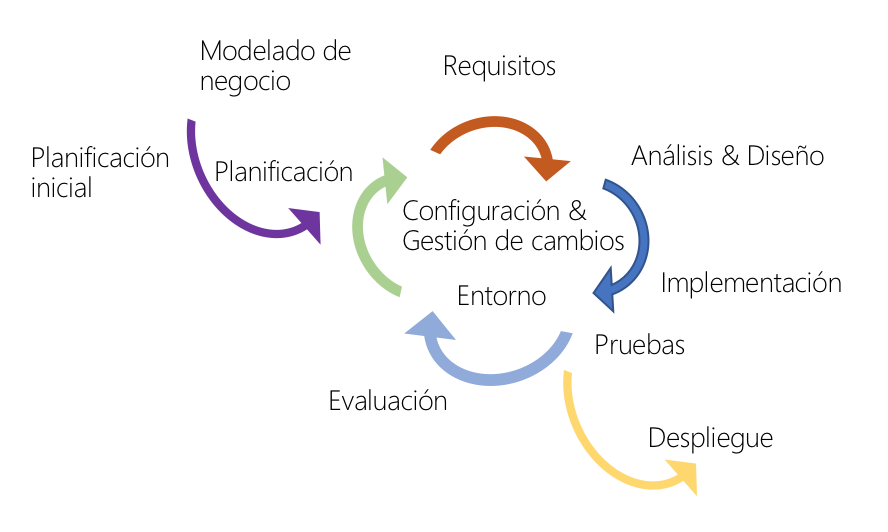
\includegraphics[width=11cm,height=6.5cm]{Images/planning/life_cycle} \\
			\label{fig:plannig-aup} 
		\end{center}  
	\end{figure}
	
	Las cuatro fases en la que la metodología \gls{aup-a} divide su ciclo de desarrollo, son:
	
	\begin{itemize}
		\item Fase de inicio: esta fase tiene como propósito definir y acordar la visión y alcance del proyecto con el cliente, identificar los posibles riesgos asociados al proyecto y proponer una planificación temporal.
		\item Fase de elaboración: se identifican, y posteriormente, se detallan los requisitos y casos de uso que permiten definir la arquitectura base del sistema, el modelo de dominio y las interacciones de las entidades con los casos de uso. También, se diseña el sistema.
		\item Fase de construcción: se implementa el sistema \textit{software} desde un punto de vista incremental, es decir, obteniendo cada vez versiones más completas y complejas basadas en las prioridades del cliente las cuales se extraen mayoritariamente en la fase anterior. También, se revisan y completan los casos de uso y se proponen cambios y mejoras a través de reuniones con el cliente.
		\item Fase de transición: el propósito de esta fase es asegurar que el sistema se encuentra en su etapa final de desarrollo ajustando errores y defectos localizados en las diferentes pruebas. Se elaboran los documentos finales (manual de instalación y configuración, manual de usuario, etc.) y se valida que el producto cumpla con las especificaciones. Por último, el sistema es desplegado en el entorno de producción.
	\end{itemize}
	
	La siguiente figura (Figura \ref{fig:plannig-aup-scheme}) muestra un esquema general de \gls{aup-a} indicando las tareas y objetivos más comunes de cada una, sin olvidar los diferentes hitos del proyecto:
	
	\begin{figure}[!ht]   
		\caption{Esquema general de fases en AUP.} 
		\begin{center} 
	 		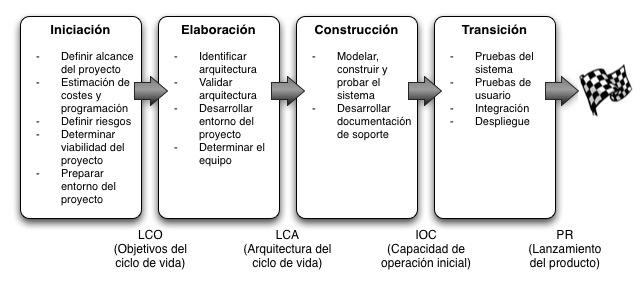
\includegraphics[width=15cm,height=6cm]{Images/planning/aup} \\
			\label{fig:plannig-aup-scheme} 
			Referencia bibliográfica: \cite{torrecilla:PUA}
		\end{center}  
	\end{figure}
	
	Cada una de las fases descritas anteriormente se puede dividir en iteraciones. Las iteraciones son una secuencia planificada de actividades (en cascada) ubicada dentro de una fase que finaliza en una versión (interna/externa). En la sección \ref{phases}. \nameref{phases}, se acometerá la división en iteraciones.			
			
	% Section
	\section{Organización del proyecto. Estructura interna}

	Otro aspecto importante en un proyecto es mostrar una visión superficial de la estructura interna de éste, referente a los roles de cada \textit{\gls{stakeholder}} participante en cada una de las fases indicadas (planificación, análisis y diseño, implementación y transición). Debido a que este proyecto ha sido realizado en el contexto de Trabajo Fin de Máster (\gls{tfm-a}), todos los roles indicados a continuación han sido llevados a cabo por una única persona, el alumno \textbf{\jesus}. \\
	
	Sí es verdad que en todo proyecto colaborativo con un equipo de trabajo, en cada fase deberían existir diferentes roles desempeñados por diferentes personas. Sin embargo en el entorno presente, al ser solamente una persona, ésta ha tenido que actuar solamente con el rol más relevante e importante de cada fase, razón por la que únicamente se muestra un rol en cada una de ellas. \\
	
	La Figura \ref{fig:plannig-organization} muestra la estructura interna para el presente proyecto.

	\begin{figure}[!ht]   
		\caption{Estructura interna.} 
		\begin{center} 
	 		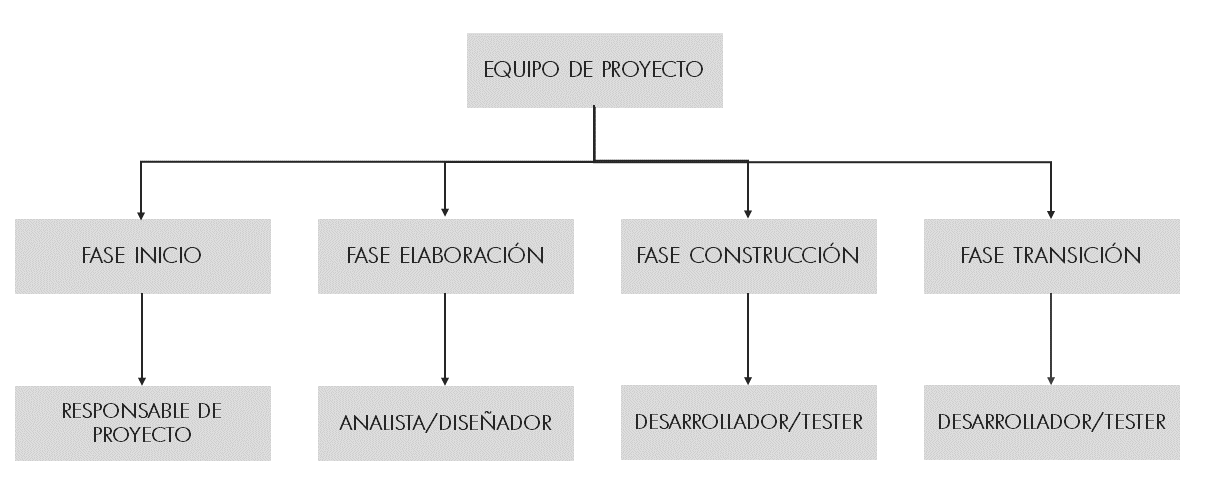
\includegraphics[width=13cm,height=5cm]{Images/planning/intern_organization} \\
			\label{fig:plannig-organization} 
		\end{center}  
	\end{figure}  

	De la imagen anterior, se pueden extraer los siguientes roles que forman la estructura interna del proyecto:

	\begin{itemize}
		\item Responsable del proyecto: graduado en Ingeniería Informática en Mención de Tecnologías de la Información (TI) y futuro graduado en Máster de Ingeniería Informática. Se encargará de ser el gerente de toda la asignación de tareas y recursos, supervisar el control, la planificación y el seguimiento del proyecto, es decir, mantener una correcta evolución del trabajo a lo largo de las iteraciones. Presenta conocimientos amplios en gestión de proyectos y en concreto en la metodología \gls{aup-a}.
		
		\item Analista de sistema: graduado en Ingeniería Informática en mención \gls{ti-a} y futuro graduado en Máster de Ingeniería Informática. Se encargará de analizar el sistema y extraer las necesidades, funcionalidades y requerimientos del sistema requeridos por el cliente. Además, se encargará de validar los requisitos, casos de uso, etc. para garantizar que se cumple todo lo solicitado.
		
		\item Ingeniero \textit{software}: también denominado diseñador. Graduado en Ingeniería Informática en mención \gls{ti-a} y futuro graduado en Máster de Ingeniería Informática. Realizará las labores de diseñar el sistema a implementar con los diferentes modelos. Presenta experiencia en el entorno de modelado \textit{software}.
		
		\item Desarrollador: graduado en Ingeniería Informática en mención \gls{ti-a} y futuro graduado en Máster de Ingeniería Informática. Se encargará de implementar y documentar el código fuente necesario para plasmar el diseño y la funcionalidad del sistema. También ejecutará baterías de prueba para asegurar el correcto funcionamiento del sistema. Presenta experiencia con la tecnología a utilizar.
		
		\item Tester: graduado en Ingeniería Informática en mención \gls{ti-a} y futuro graduado en Máster de Ingeniería Informática. Se encargará de la medición y aseguramiento de la calidad de los procesos utilizados para crear un producto de calidad ajustándose a las necesidades específicas y a los planes establecidos anteriormente. Ejecutará exhaustivamente pruebas finales funcionales, de diseño y técnicas, todas ellas encaminadas a la detección de errores durante el proceso de desarrollo del producto.		
	\end{itemize}
		
	% Section
	\section{Plan de fases} \label{phases}
	
	Todo proyecto debe comenzar con la elaboración de una planificación para poder tener una visión superficial de la distribución temporal y de recursos del mismo. Un buen artefacto que ayuda y facilita la planificación temporal es el plan de fases junto al plan de iteraciones. El plan de fases se elabora durante la fase de inicio de \gls{aup-a} y se corresponde con una planificación de alto nivel donde se puede observar claramente las diferentes fases de las que consta el proyecto así como el número de iteraciones en cada una de ellas, fechas estimadas de las mismas y objetivos propuestos. \\
	
	Debido a que su elaboración se realiza al comienzo de un proyecto, se debe tener en cuenta que los períodos de tiempo indicados para cada fase son estimados. Estos períodos podrán ser modificados y/o sufrir retrasos por diversas dificultades y riesgos que puedan manifestarse a lo largo del desarrollo. Centrándonos en el plan de trabajo, la dimensión temporal de realización de este proyecto es de aproximadamente 9 meses (39 semanas) con una comunicación continuada del progreso del proyecto (aproximadamente cada 2-3 semanas) a mi tutor para permitir un seguimiento minucioso y una retroalimentación por parte de él. \\
	
	\textbf{Concluido el \gls{tfm-a}}, se puede afirmar que los intervalos de fechas expuestos han coincidido en una alta probabilidad con el trabajo real realizado, no presentando retrasos ni inconvenientes con respecto a la planificación inicial estimada y sí logrando un mínimo adelanto en la finalización.\\
			
	A continuación, se muestra la distribución porcentual temporal y de esfuerzo estimada de cada fase y el plan de fases del proyecto: \\
		
	% Percentage estimate of each phase
	\begin{longtable}{|m{4cm}|m{2cm}|m{2cm}|m{2cm}|m{2cm}|}
		\hline
			
		\multicolumn{1}{|>{\columncolor{Gainsboro}}c|}{} & \multicolumn{1}{>{\columncolor{Gainsboro}}c|}{\textsc{Inicio}} & \multicolumn{1}{>{\columncolor{Gainsboro}}c|}{\textsc{Elaboración}} & \multicolumn{1}{>{\columncolor{Gainsboro}}c|}{\textsc{Construcción}} & \multicolumn{1}{>{\columncolor{Gainsboro}}c|}{\textsc{Transición}}
		\\ \hline
		
		\multicolumn{1}{|p{2.5cm}|}{\textbf{Esfuerzo}} & \multicolumn{1}{c|}{5\%} & \multicolumn{1}{c|}{20\%} & \multicolumn{1}{c|}{65\%} & \multicolumn{1}{c|}{10\%} 
		\\ \hline
		
		\multicolumn{1}{|l|}{\textbf{Tiempo}} & \multicolumn{1}{c|}{10\%} & \multicolumn{1}{c|}{15,5\%} & \multicolumn{1}{c|}{59\%} & \multicolumn{1}{c|}{15,5\%} 
		\\ \hline
			
		\caption{Estimación porcentual de cada fase}
	\end{longtable}
		
	% New page	
	\newpage
		
	% Plan of phases
	\begin{longtable}{|m{4cm}|m{2cm}|m{2cm}|m{2cm}|m{2cm}|}
		\hline
			
		\multicolumn{1}{|>{\columncolor{Gainsboro}}c|}{\textsc{Fase}} & \multicolumn{1}{>{\columncolor{Gainsboro}}c|}{\textsc{Iteraciones}} & \multicolumn{1}{>{\columncolor{Gainsboro}}c|}{\textsc{Fecha Inicio}} & \multicolumn{1}{>{\columncolor{Gainsboro}}c|}{\textsc{Fecha Final}} & \multicolumn{1}{>{\columncolor{Gainsboro}}c|}{\textsc{Duración}} 
		\\ \hline
		
		\multicolumn{1}{|p{3cm}|}{\textbf{Inicio}} & \multicolumn{1}{c|}{1} & \multicolumn{1}{c|}{04/12/2017} & \multicolumn{1}{c|}{31/12/2017} & \multicolumn{1}{c|}{4 semanas} 
		\\ \hline
		
		\multicolumn{1}{|p{3cm}|}{\textbf{Elaboración}} & \multicolumn{1}{c|}{1} & \multicolumn{1}{c|}{01/01/2018} & \multicolumn{1}{c|}{11/02/2018} & \multicolumn{1}{c|}{6 semanas} 
		\\ \hline
		
		\multicolumn{1}{|p{3cm}|}{\textbf{Construcción}} & \multicolumn{1}{c|}{2} & \multicolumn{1}{c|}{12/02/2018} & \multicolumn{1}{c|}{22/07/2018} & \multicolumn{1}{c|}{23 semanas} 
		\\ \hline

		\multicolumn{1}{|p{3cm}|}{\textbf{Transición}} & \multicolumn{1}{c|}{1} & \multicolumn{1}{c|}{23/07/2018} & \multicolumn{1}{c|}{31/08/2018} & \multicolumn{1}{c|}{6 semanas} 
		\\ \hline
		
		\caption{Plan de fases del proyecto}
	\end{longtable}
	
	
	El final de cada fase está marcado por un hito principal e hito secundario en el caso de final de iteración. En este proyecto, todo final de fase se corresponde con un final de iteración y a continuación se detalla a grandes rasgos el trabajo desarrollado en cada una de ellas permitiendo obtener una perspectiva del esquema seguido: \\
		
	% Phases and milestones of the project 
	\begin{longtable}{|m{4cm}|m{2cm}|}
		\hline
		
		\multicolumn{1}{|>{\columncolor{Gainsboro}}c|}{\textsc{Fase}} & \multicolumn{1}{>{\columncolor{Gainsboro}}c|}{\textsc{Hito}}
		\\ \hline

		\multicolumn{1}{|p{3cm}|}{\textbf{Inicio}} & \multicolumn{1}{p{13cm}|}{Se ha estudiado el problema propuesto y la visión general de la solución del proyecto plasmando de esta manera la definición y alcance del proyecto, la planificación inicial, la estimación de costes y la gestión de riesgos. También, se analizó el estudio de arte de las tecnologías \Gls{blockchain} (\gls{blockchain-a}), profundizando en \gls{hyperledgerfabric} (\gls{hyperledgerfabric-a}). La finalización de esta fase corresponde al \textbf{hito 1}.} 
		\\ \hline

		\multicolumn{1}{|p{3cm}|}{\textbf{Elaboración}} & \multicolumn{1}{p{13cm}|}{Una vez definido con mayor exactitud el proyecto en sí, se ha realizado todo el proceso de análisis y diseño del mismo para identificar los requisitos, actores, casos de uso, modelo de dominio, diseño de la arquitectura física del sistema, etc. La finalización de esta fase corresponde al \textbf{hito 2}.}
		\\ \hline
		
		\multicolumn{1}{|p{3cm}|}{\textbf{Construcción}} & \multicolumn{1}{p{13cm}|}{Dos iteraciones componen esta fase en la cual al final de cada una se produce una versión funcional e incremental del sistema. Durante la primera iteración se ha revisado y completado la definición de requisitos y casos de uso así como el diseño. En esta iteración\footnote{El anexo \ref{trello}. \nameref{trello} muestra la gestión de tareas para la codificación del proyecto.}, en primer lugar se preparó el entorno de trabajo y se definieron las diferentes partes de las que iba a constar el proyecto, implementando el componente de configuración de la \gls{raspberry} (\gls{raspberry-a}), de monitorización de sucesos y de desencriptación. En la segunda iteración, se revisaron algunos errores que aparecieron a causa de la implementación durante la primera iteración y se desplegó la \gls{blockchain-a} de \gls{hyperledgerfabric-a} definiendo la red de negocio y el sistema web. El \textbf{hito 3} y el \textbf{hito 4} se corresponden con el final de cada iteración, marcando también este último el final de fase.} 
		\\ \hline
		
		\multicolumn{1}{|p{3cm}|}{\textbf{Transición}} & \multicolumn{1}{p{13cm}|}{En esta última fase se han solucionado aquellos errores presentados en la segunda iteración (hito 4) de la fase de construcción y se ha llevado a cabo la ejecución de la batería de pruebas final. Además, se ha redactado la memoria, se han finalizado los manuales de usuario y de configuración del sistema y se ha preparado la versión definitiva del proyecto. La finalización de esta fase se corresponde con el \textbf{hito 5} donde se entrega el producto final junto con la documentación adicional.}
		\\ \hline

		\caption{Descripción de fases e hitos del proyecto}
	\end{longtable}
	
	% Section
	\section{Plan de iteraciones}
				
	Indicado anteriormente, una iteración es una secuencia de actividades dentro de una fase con un plan establecido y unos criterios de evaluación, cuyo resultado es una versión interna/externa (hito secundario). Mientras que hito se puede definir como el punto de control en los cuales los participantes del proyecto revisan el progreso de éste. \\
	
	En este apartado se desglosa cada una de las 5 iteraciones definidas, pudiendo observar a través de la planificación temporal tanto del calendario como del \gls{gantt} los siguientes detalles: actividades englobadas, tiempo invertido en cada una (definido en días), recursos asignados y relaciones de precedencia las cuales condicionan el inicio en función de la predecesora. \\
	
	En el momento de realizar la planificación inicial del proyecto para cada iteración se estableció un calendario laboral\footnote{En la herramienta \textit{Microsoft Project 2016} se ha creado un calendario con nombre ``\textit{calendar}'' donde se ha definido la fecha de comienzo de cada iteración, el horario de trabajo, los días festivos y los recursos humanos involucrados en el proyecto junto con su coste por hora asociado.} compuesto por:
	
	\begin{itemize}
		\item \textbf{Días laborables}
		\begin{itemize}
			\item Lunes-Viernes. Jornada laboral de 4 horas al día\footnote{La dedicación al \gls{tfm-a} ha sido parcial y no completa debido a que el recurso se encuentra en actividad laboral al momento de desarrollar este proyecto.} con el siguiente horario:
			\begin{itemize}
				\item De 17:00 a 21:00
			\end{itemize}
			\item Sábados. Jornada laboral de 4 horas al día con el siguiente horario:
			\begin{itemize}
				\item De 10:00 a 14:00
			\end{itemize}
		\end{itemize}
		
		% New page
		\newpage
		\item \textbf{Días no laborables} 
		\begin{itemize}
			\item Domingo y festivos. Los festivos definidos han sido:
			\begin{multicols}{2}
				\begin{itemize}
					\item Día de la Constitución - 06/12/2017
					\item Día de la Inmaculada - 08/12/2017
					\item Natividad del Señor - 25/12/2017
					\item Año Nuevo - 01/01/2018
					\item Epifanía del Señor - 06/01/2018
					\item Jueves Santo - 29/03/2018
					\item Viernes Santo - 30/03/2018
					\item Fiesta del Trabajo - 01/05/2018
					\item Día de la Comunidad de Madrid - 02/05/2018
					\item San Isidro - 15/05/2018
					\item Asunción de la virgen - 15/08/2018
				\end{itemize}
			\end{multicols}
		\end{itemize}
	\end{itemize}
		 
	Para evitar al lector tener que instalar \textit{software} adicional para la visión de la planificación de cada una de las cinco iteraciones\footnote{Los ficheros con nombre \textit{Plan\_IteracionX.mpp}, representando el carácter \textit{X} un valor numérico entre 1-5, ubicados dentro del repositorio de código se corresponden con el plan de iteración de cada una de ellas.}, a continuación se muestran los calendarios y \glspl{gantt}: 
	
	\begin{itemize}

		\item \textbf{Iteración 1:} 24 días en total\footnote{Sin contar los días no laborables: Domingo.} (21 días laborables + 3 días festivos). % TODO Revisar las acciones de cada calendario
		
		\begin{figure}[!ht]   
			\caption{Calendario de la fase de inicio - Iteración 1.} 
			\begin{center} 
		 		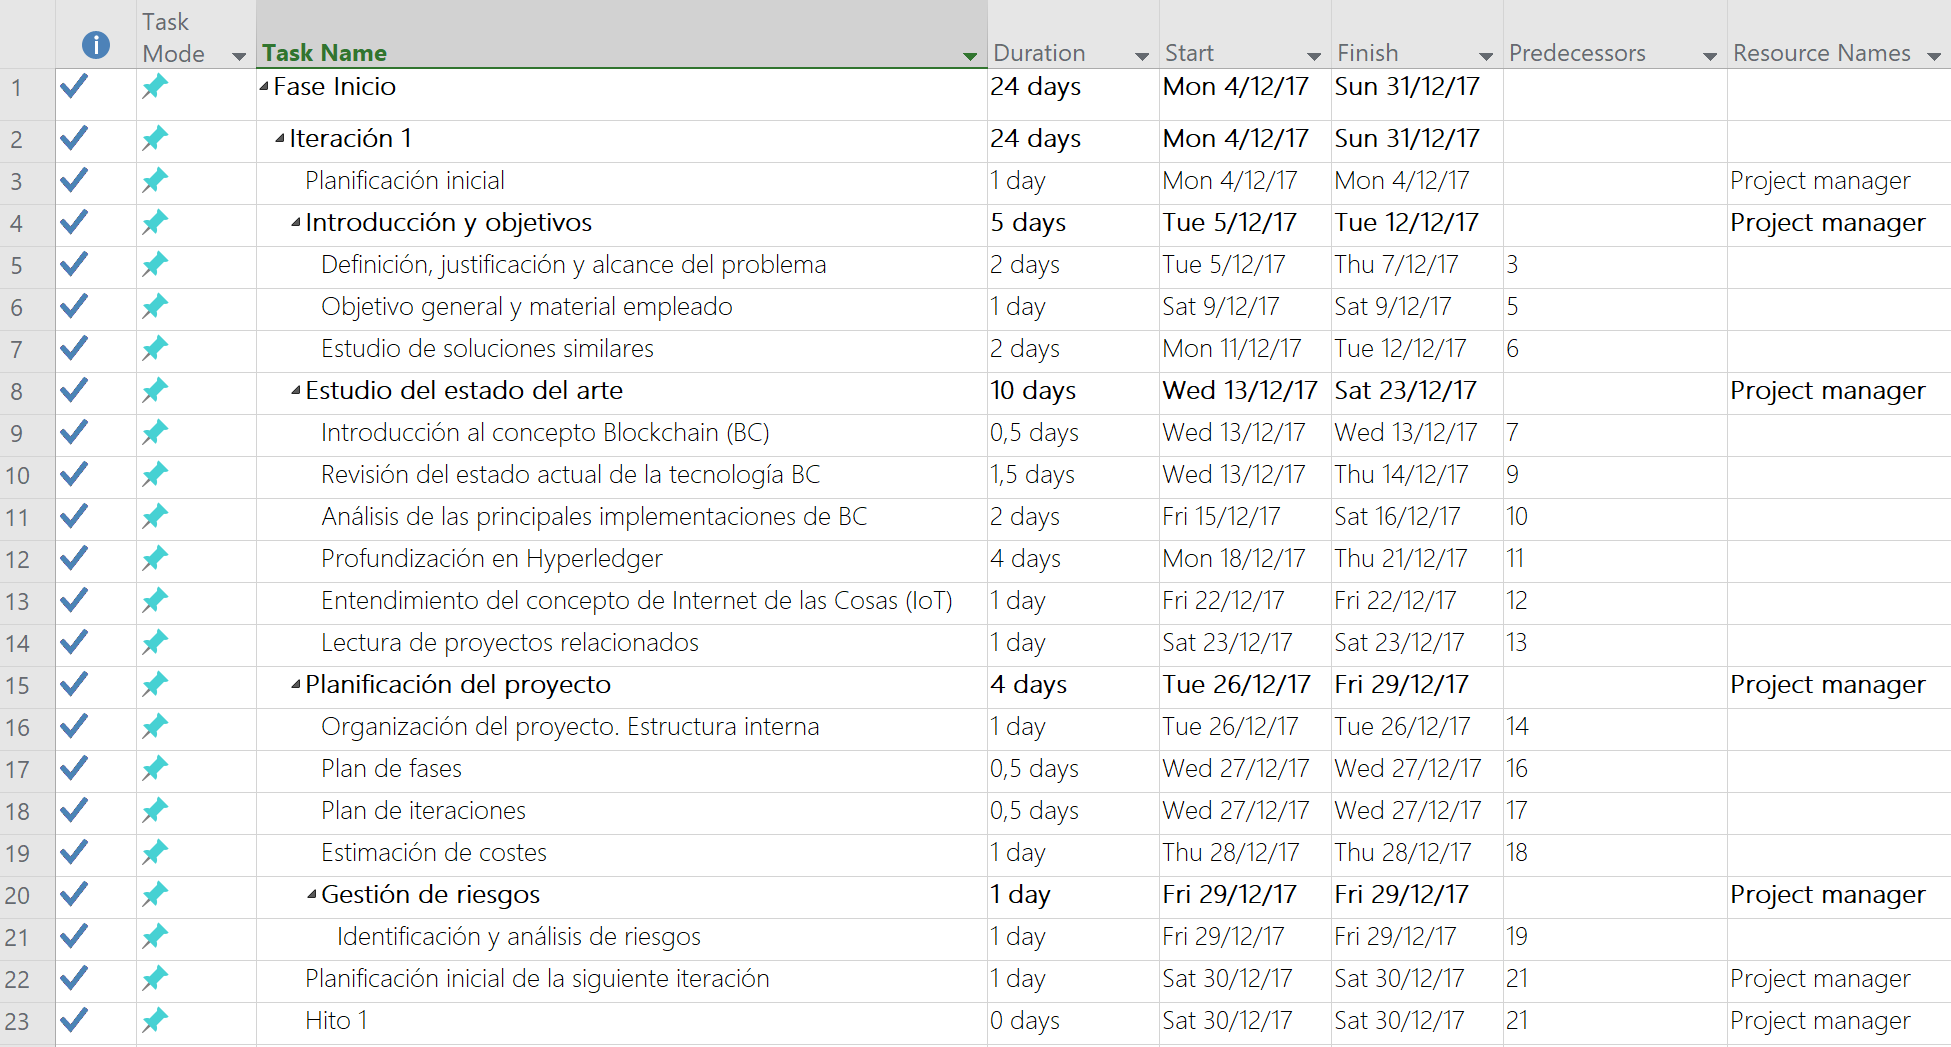
\includegraphics[width=16cm,height=9.4cm]{Images/planning/iterations/It1_calendar} \\
				\label{fig:planning-it1-calendar} 
			\end{center}  
		\end{figure}  
		
		\begin{figure}[!ht]   
			\caption{Diagrama de Gantt de la fase de inicio - Iteración 1.} 
			\begin{center} 
		 		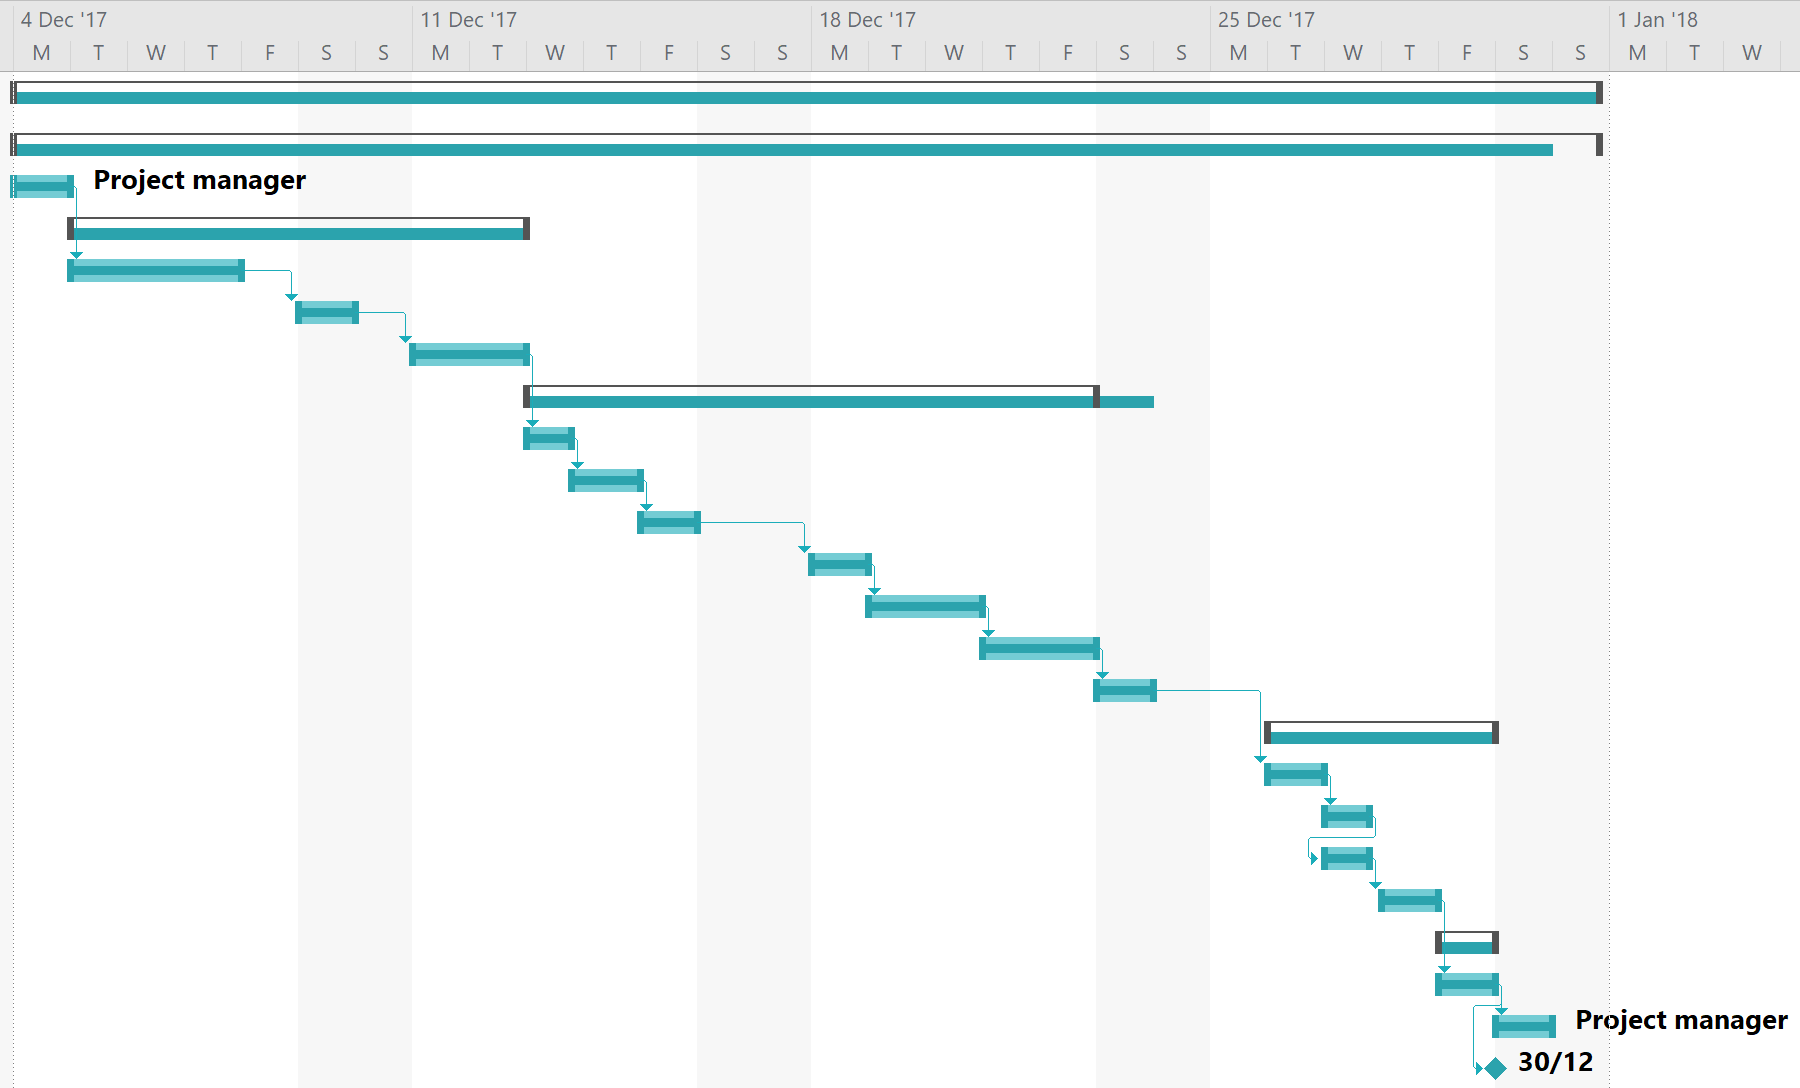
\includegraphics[width=16cm,height=8cm]{Images/planning/iterations/It1_gantt} \\
				\label{fig:planning-it1-gantt} 
			\end{center}  
		\end{figure}  
		
		% New page
		\newpage
		\item \textbf{Iteración 2:} 36 días en total (34 días laborables + 2 días festivos).
		
		\begin{figure}[!ht]   
			\caption{Calendario de la fase de elaboración - Iteración 2.} 
			\begin{center} 
		 		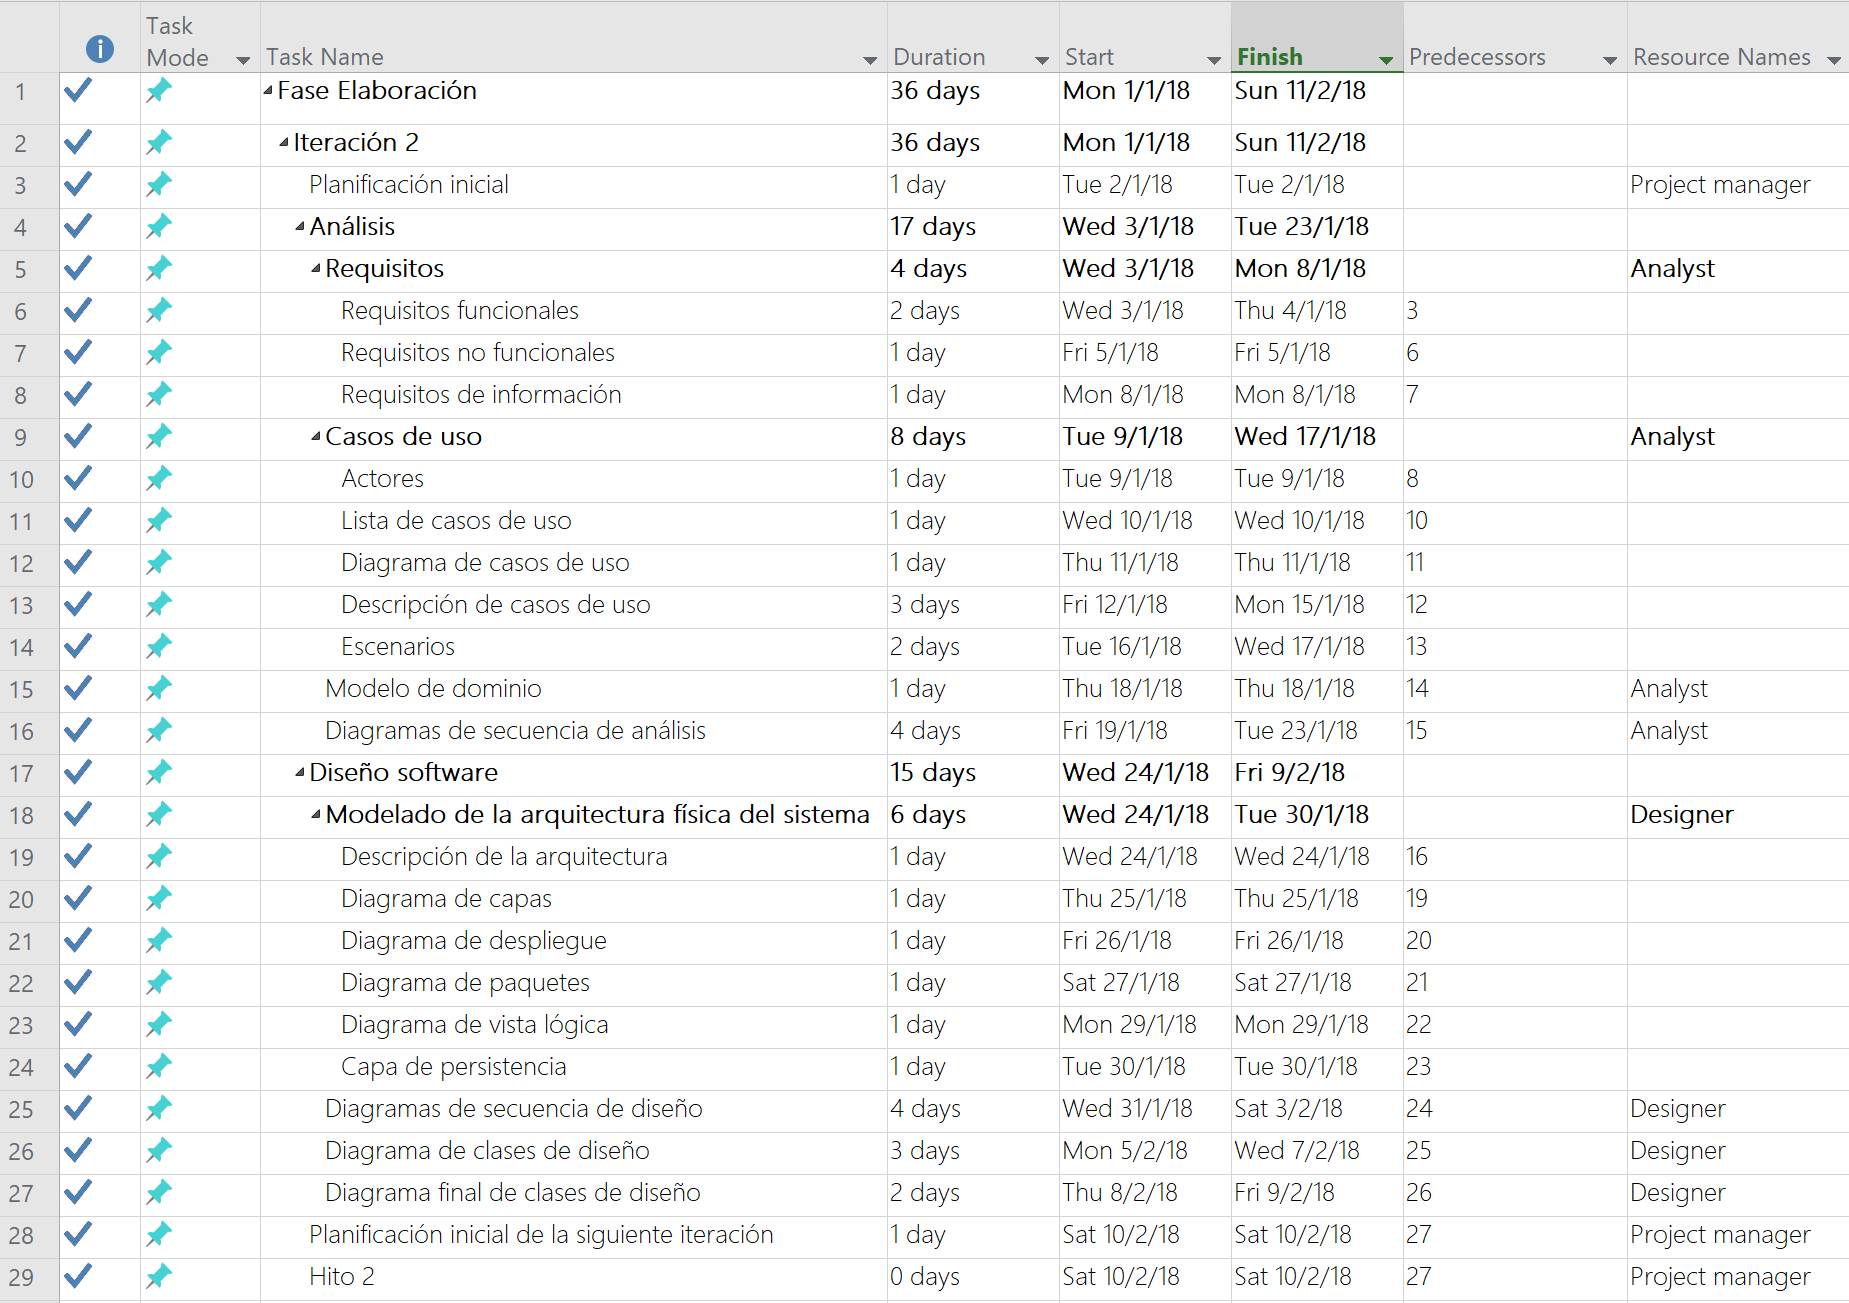
\includegraphics[width=16cm,height=10cm]{Images/planning/iterations/It2_calendar} \\
				\label{fig:planning-it2-calendar} 
			\end{center}  
		\end{figure}  
		
		\begin{figure}[!ht]   
			\caption{Diagrama de Gantt de la fase de elaboración - Iteración 2.} 
			\begin{center} 
		 		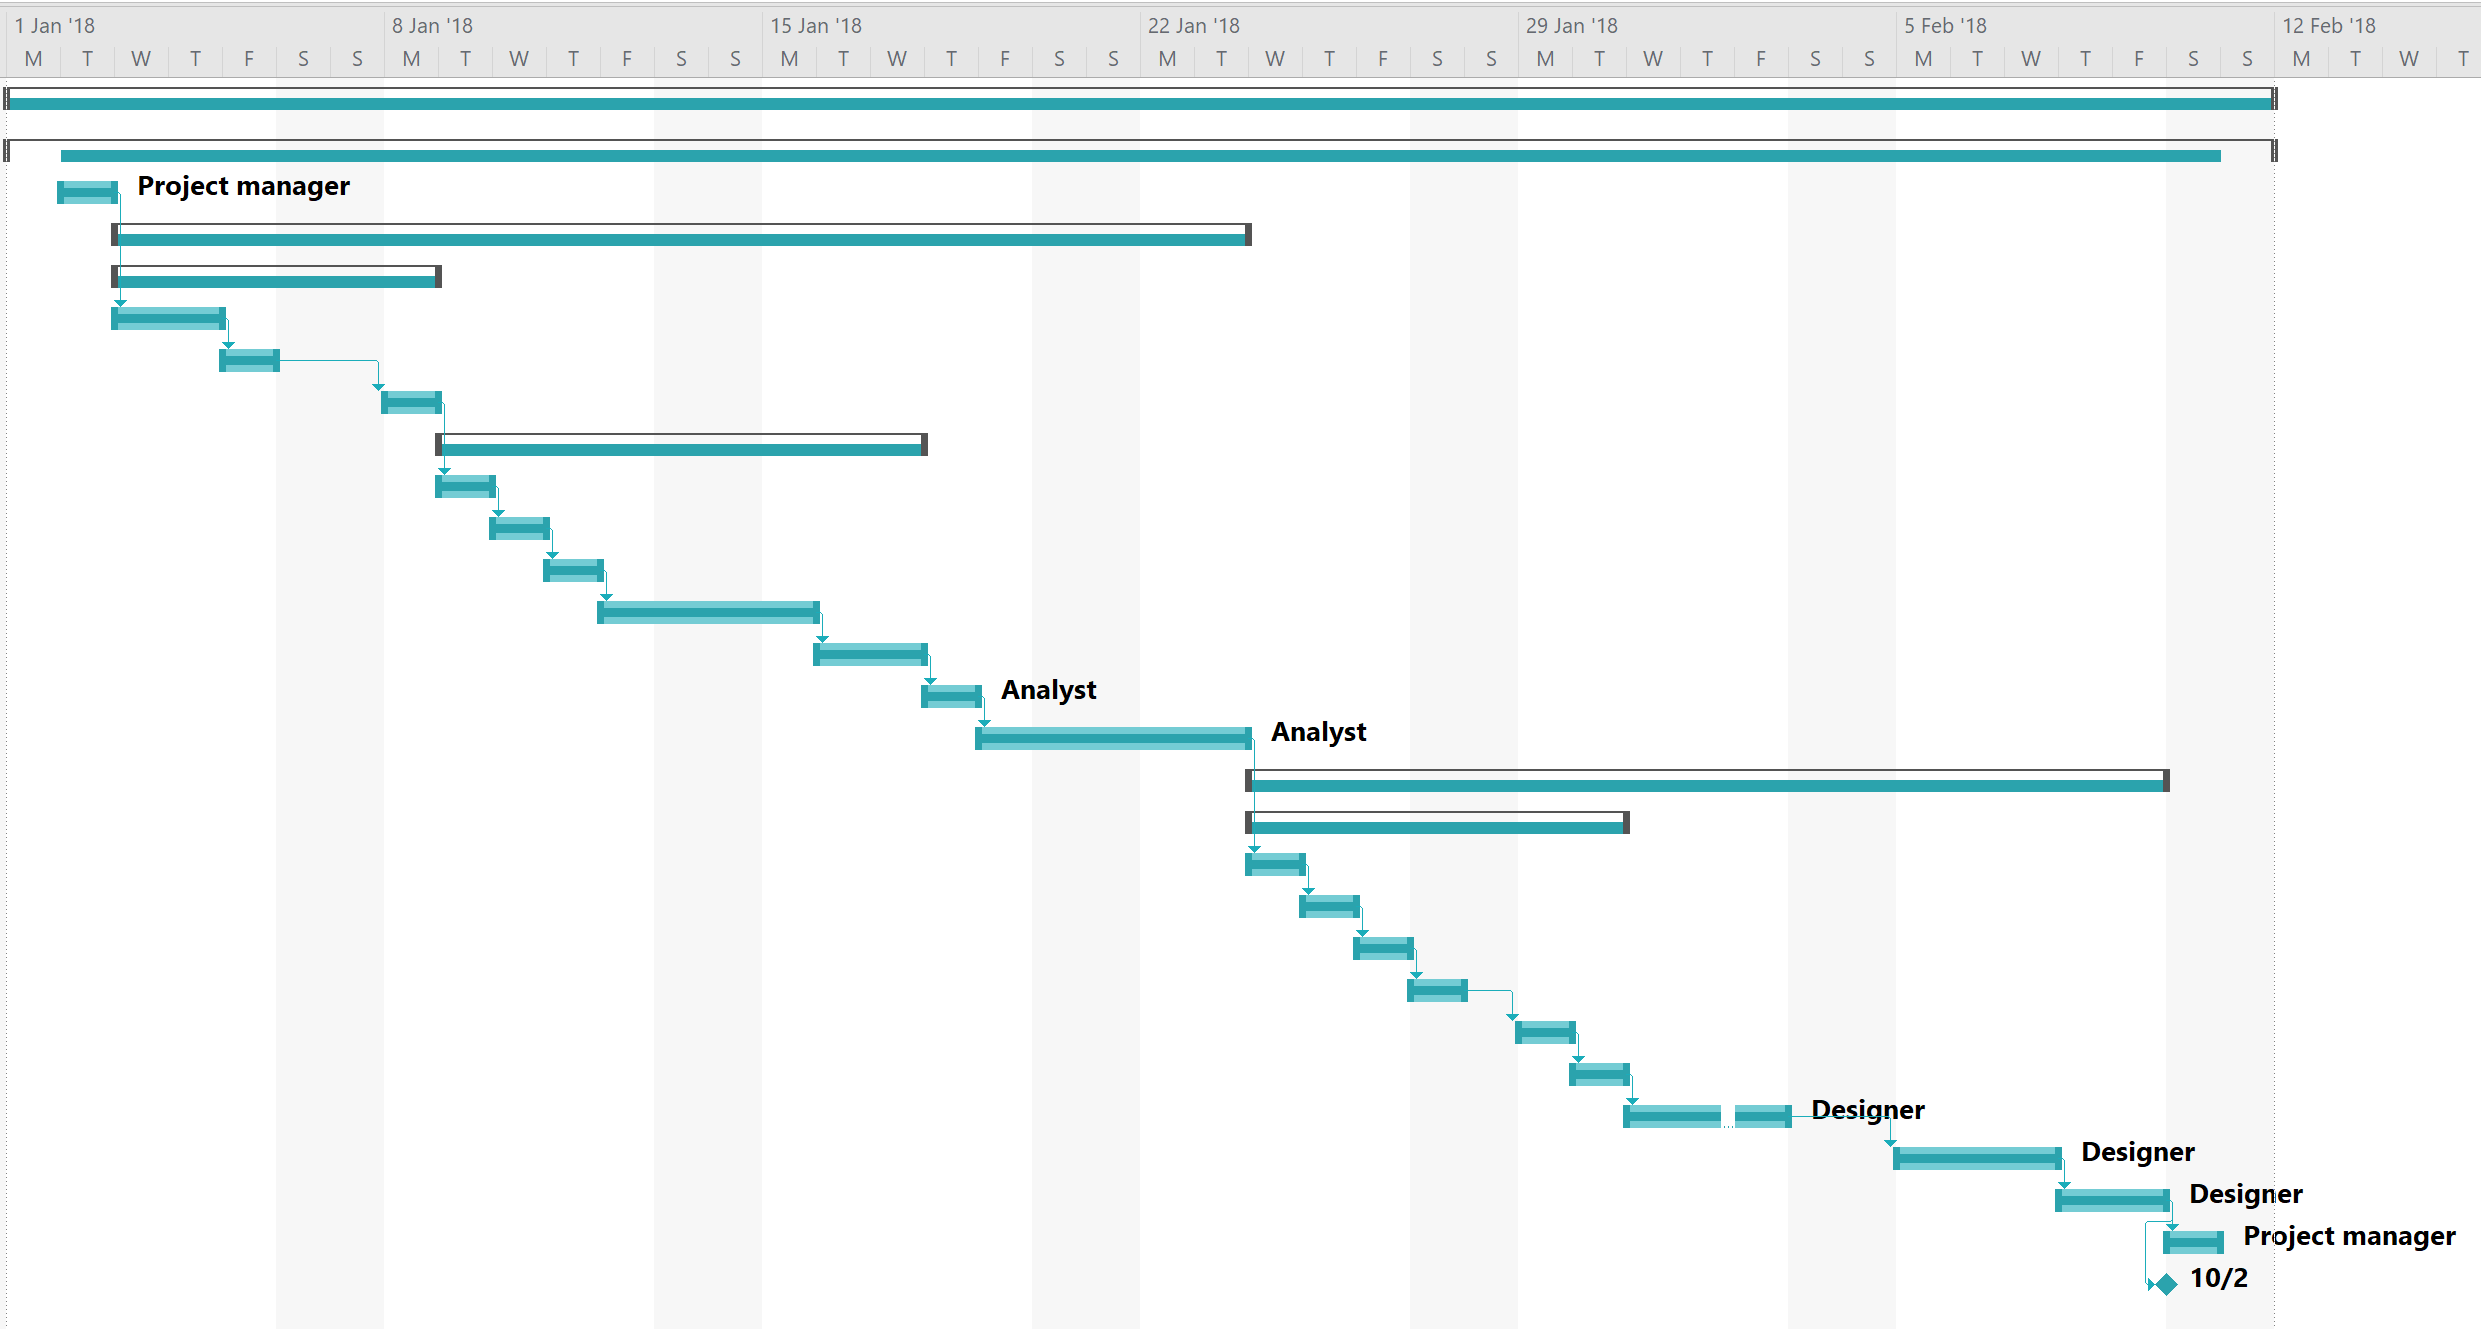
\includegraphics[width=16cm,height=9cm]{Images/planning/iterations/It2_gantt} \\
				\label{fig:planning-it2-gantt} 
			\end{center}  
		\end{figure}  
		
		\item \textbf{Iteración 3:} 72 días en total (68 días laborables + 4 días festivos).
		
		\begin{figure}[!ht]   
			\caption{Calendario de la fase de construcción - Iteración 3.} 
			\begin{center} 
		 		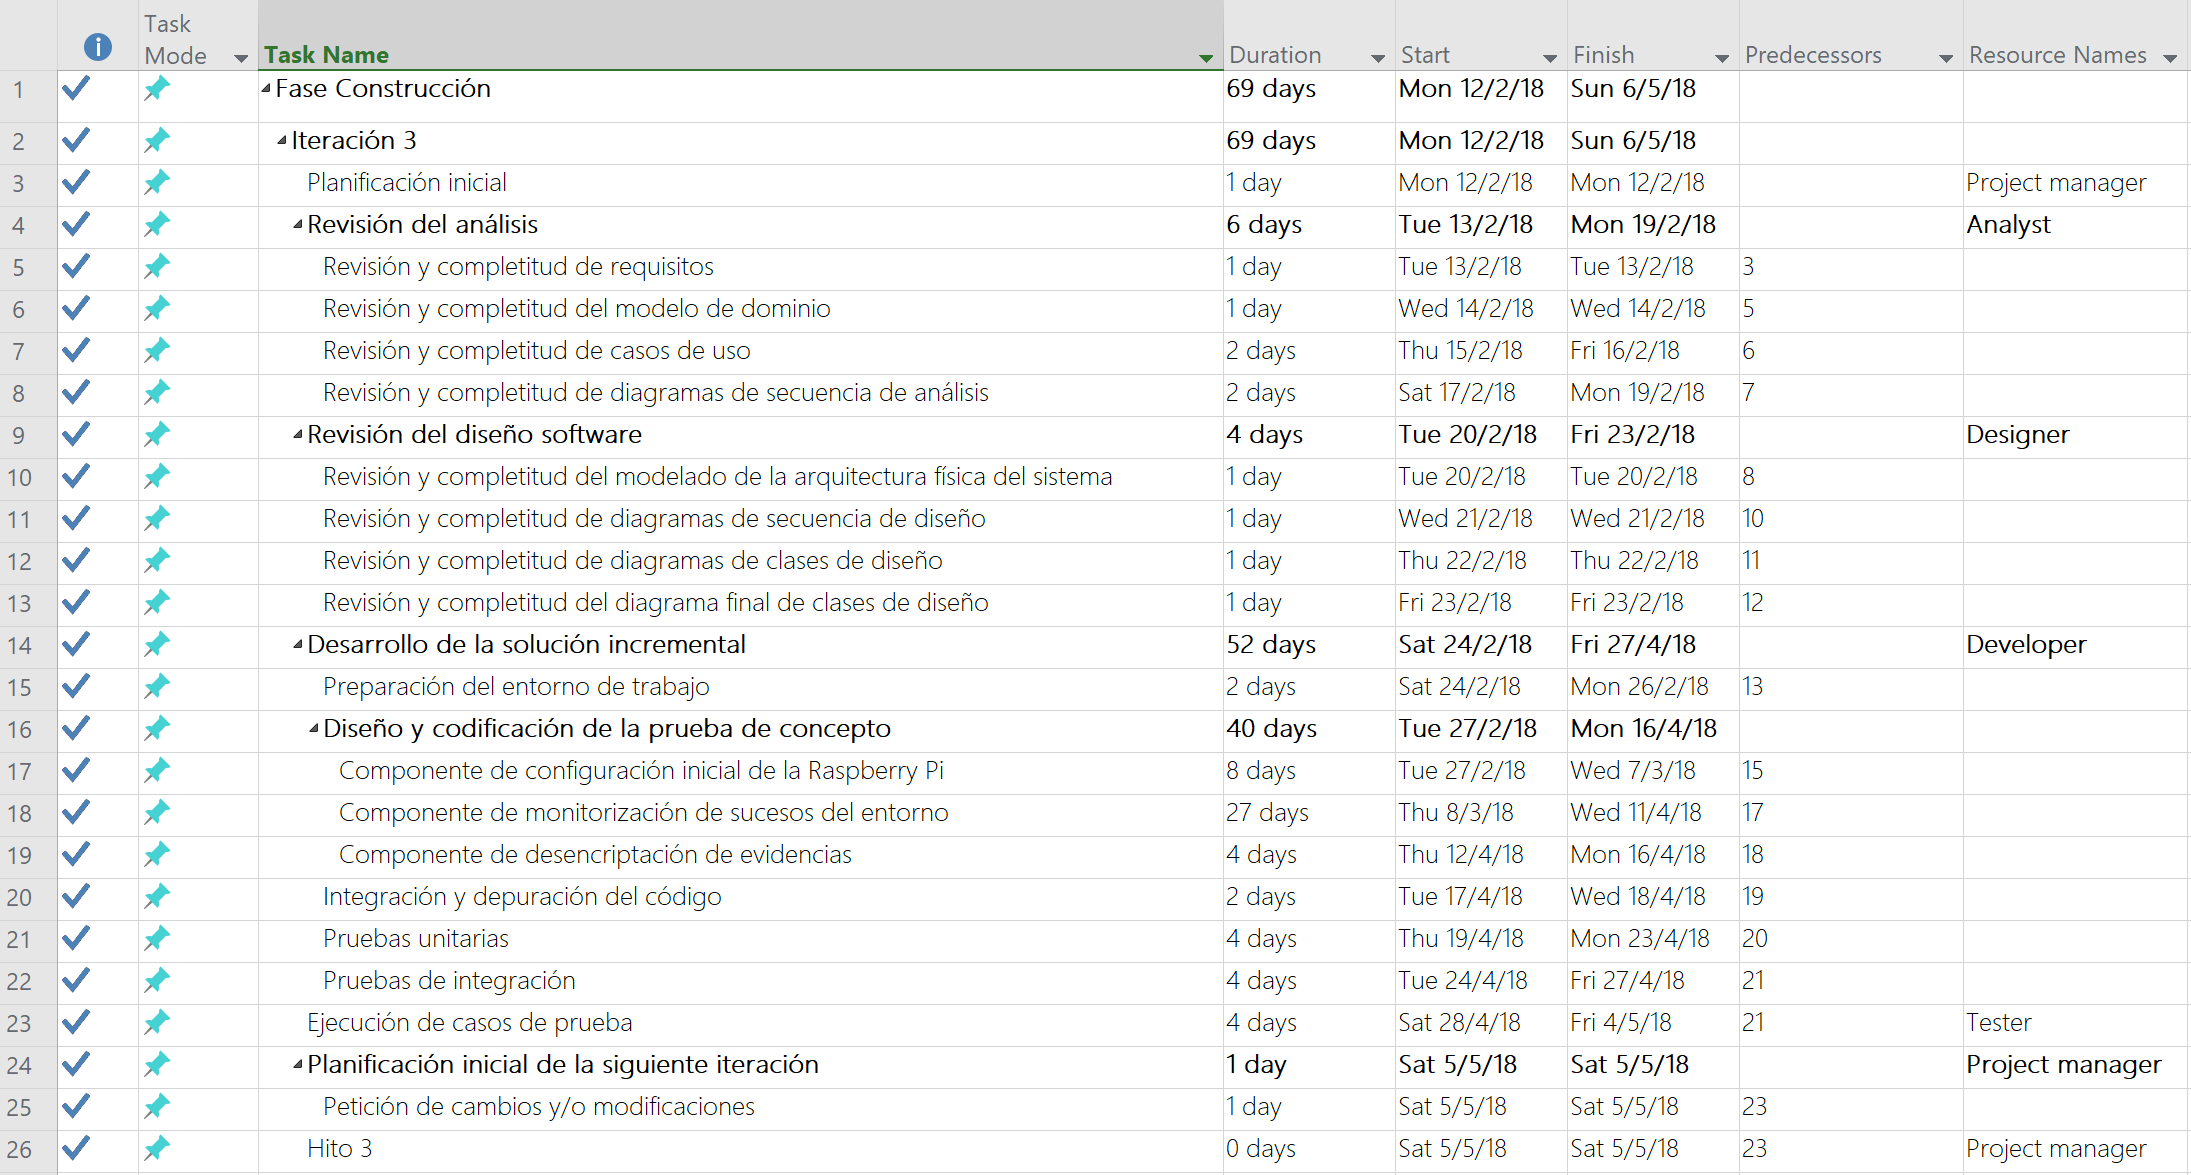
\includegraphics[width=16cm,height=9.2cm]{Images/planning/iterations/It3_calendar} \\
				\label{fig:planning-it3-calendar} 
			\end{center}  
		\end{figure}  
		
		\begin{figure}[!ht]   
			\caption{Diagrama de Gantt de la fase de construcción - Iteración 3.} 
			\begin{center} 
		 		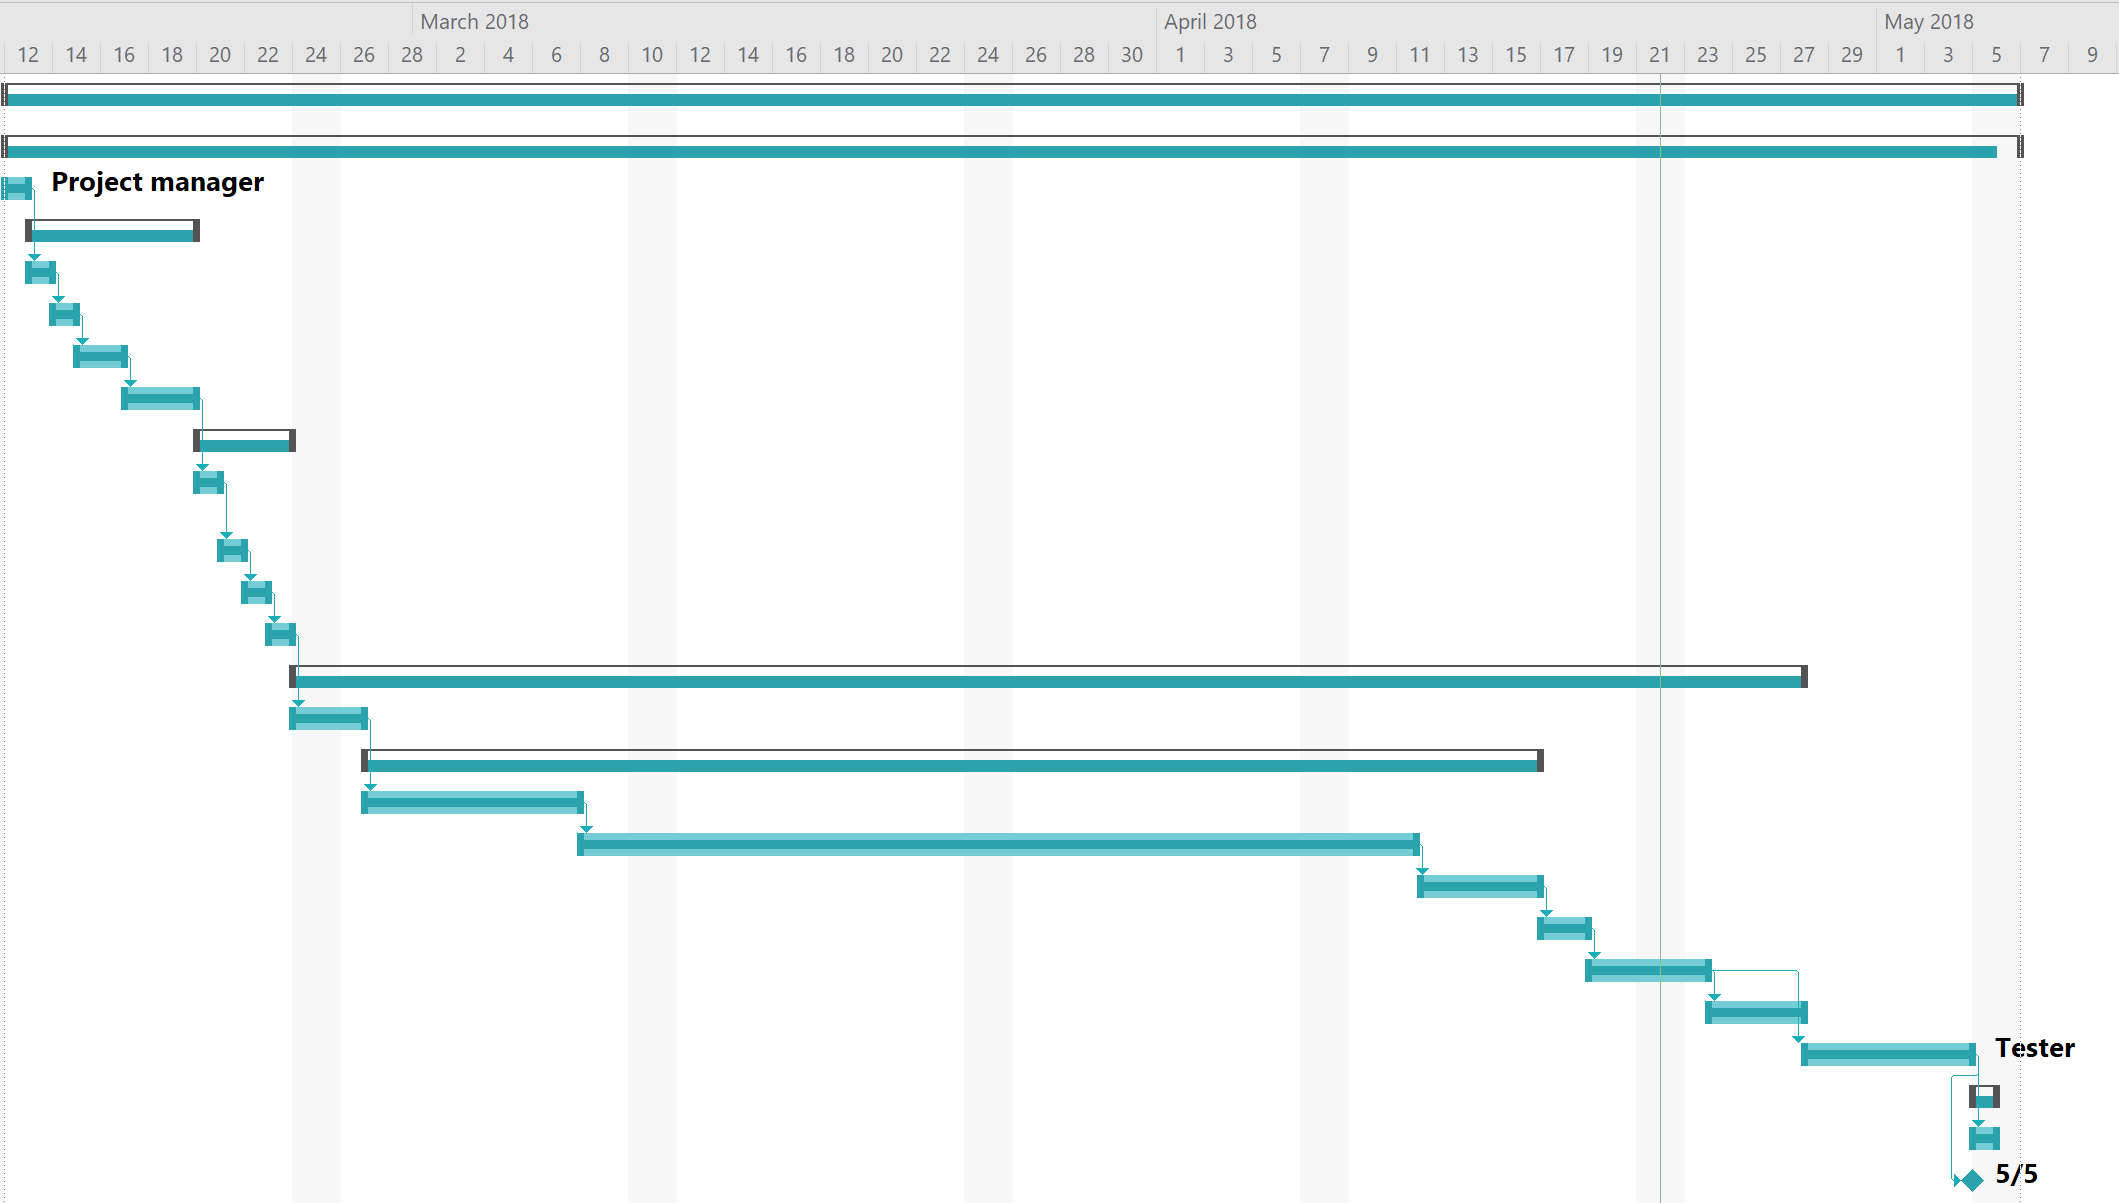
\includegraphics[width=16cm,height=9cm]{Images/planning/iterations/It3_gantt} \\
				\label{fig:planning-it3-gantt} 
			\end{center}  
		\end{figure}  
		
		\item \textbf{Iteración 4:} 66 días en total (65 días laborables + 1 día festivo).
		
		\begin{figure}[!ht]   
			\caption{Calendario de la fase de construcción - Iteración 4.} 
			\begin{center} 
		 		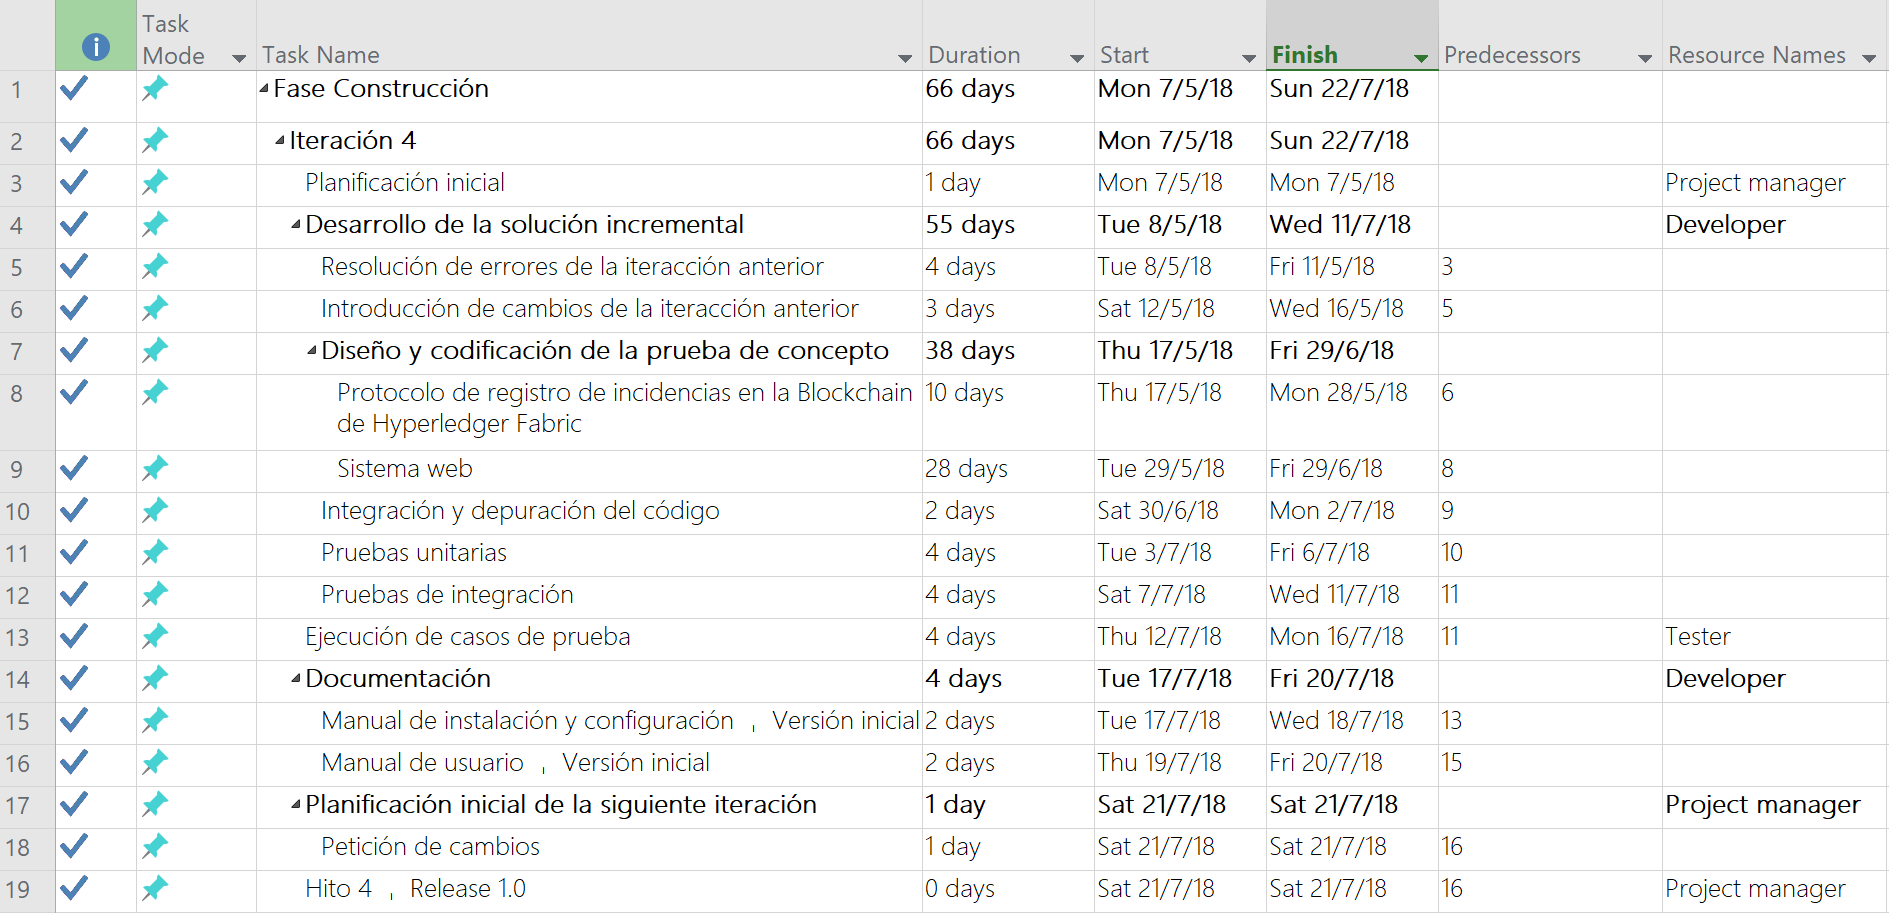
\includegraphics[width=16cm,height=8cm]{Images/planning/iterations/It4_calendar} \\
				\label{fig:planning-it4-calendar} 
			\end{center}  
		\end{figure}  
		
		\begin{figure}[!ht]   
			\caption{Diagrama de Gantt de la fase de construcción - Iteración 4.} 
			\begin{center} 
		 		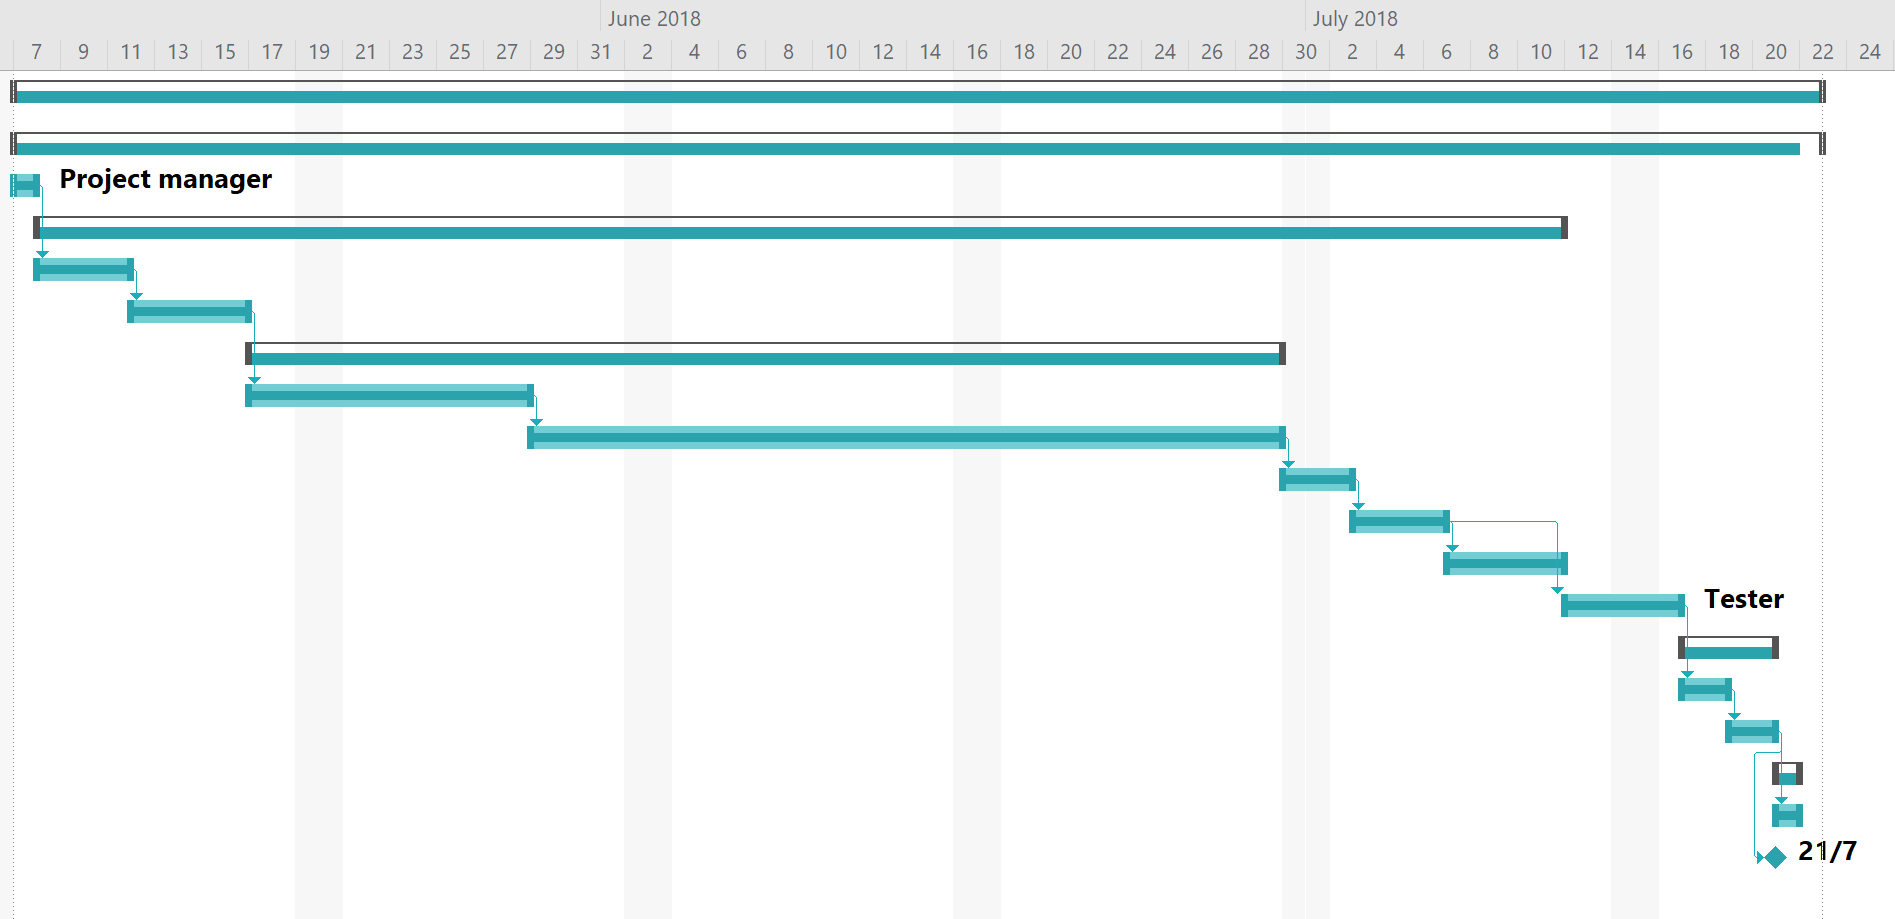
\includegraphics[width=16cm,height=8cm]{Images/planning/iterations/It4_gantt} \\
				\label{fig:planning-it4-gantt} 
			\end{center}  
		\end{figure}  

		% New page
		\newpage
		\item \textbf{Iteración 5:} 35 días en total (34 días laborables + 1 día festivo).
		
		\begin{figure}[!ht]   
			\caption{Calendario de la fase de transición - Iteración 5.} 
			\begin{center} 
		 		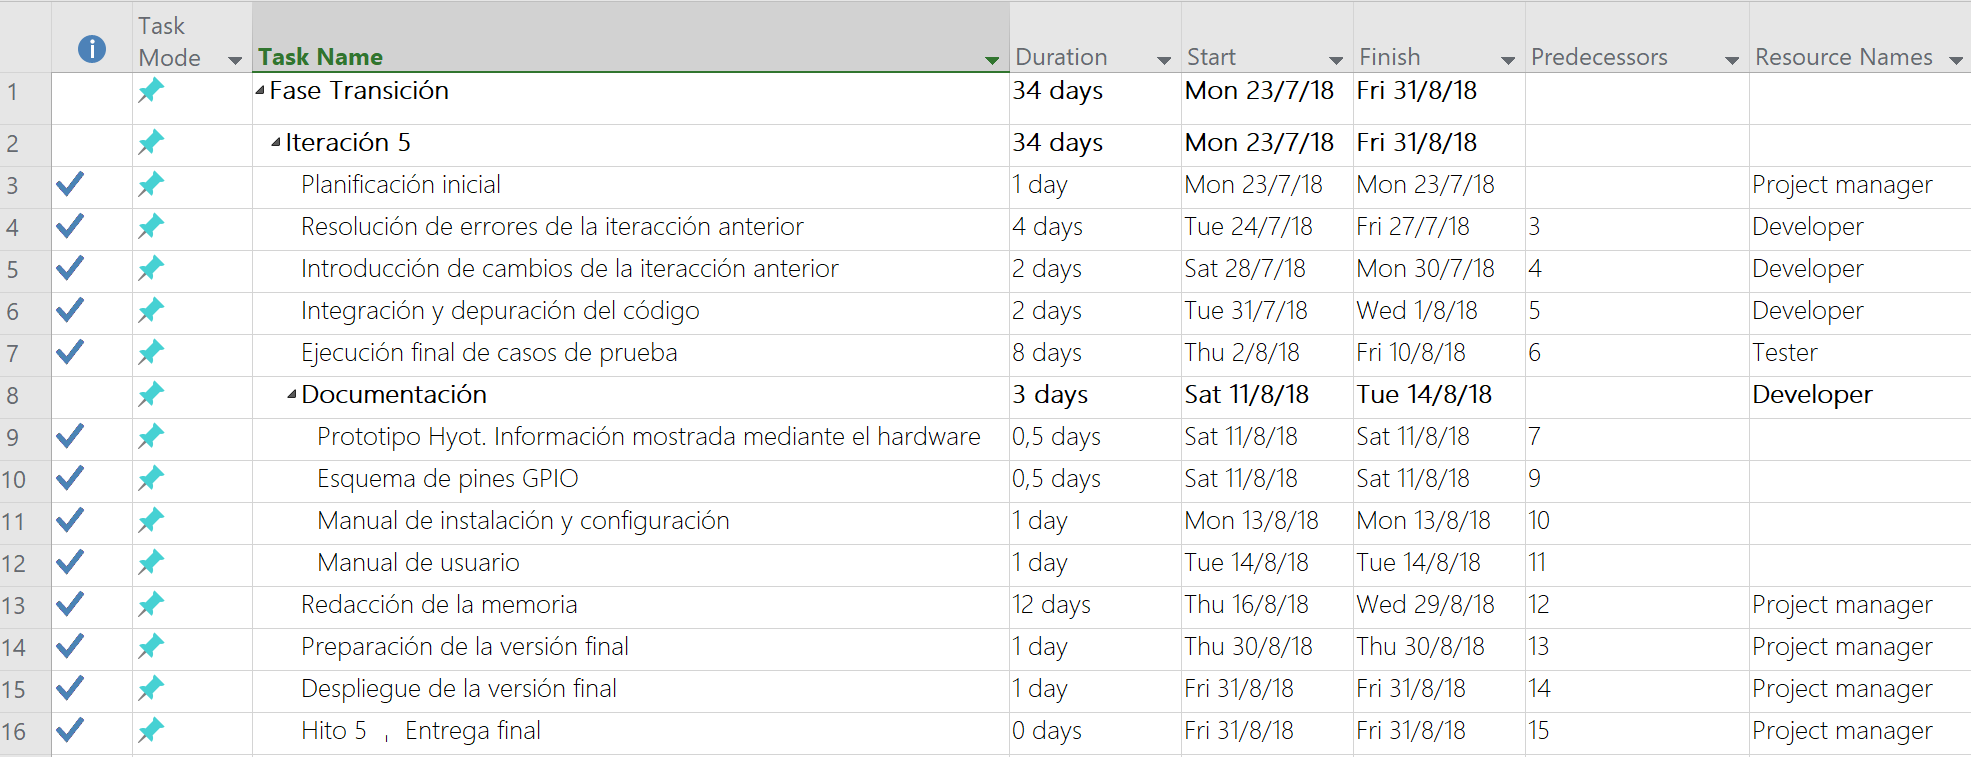
\includegraphics[width=16cm,height=7.5cm]{Images/planning/iterations/It5_calendar} \\
				\label{fig:planning-it5-calendar} 
			\end{center}  
		\end{figure}  
		
		\begin{figure}[!ht]   
			\caption{Diagrama de Gantt de la fase de transición - Iteración 5.} 
			\begin{center} 
		 		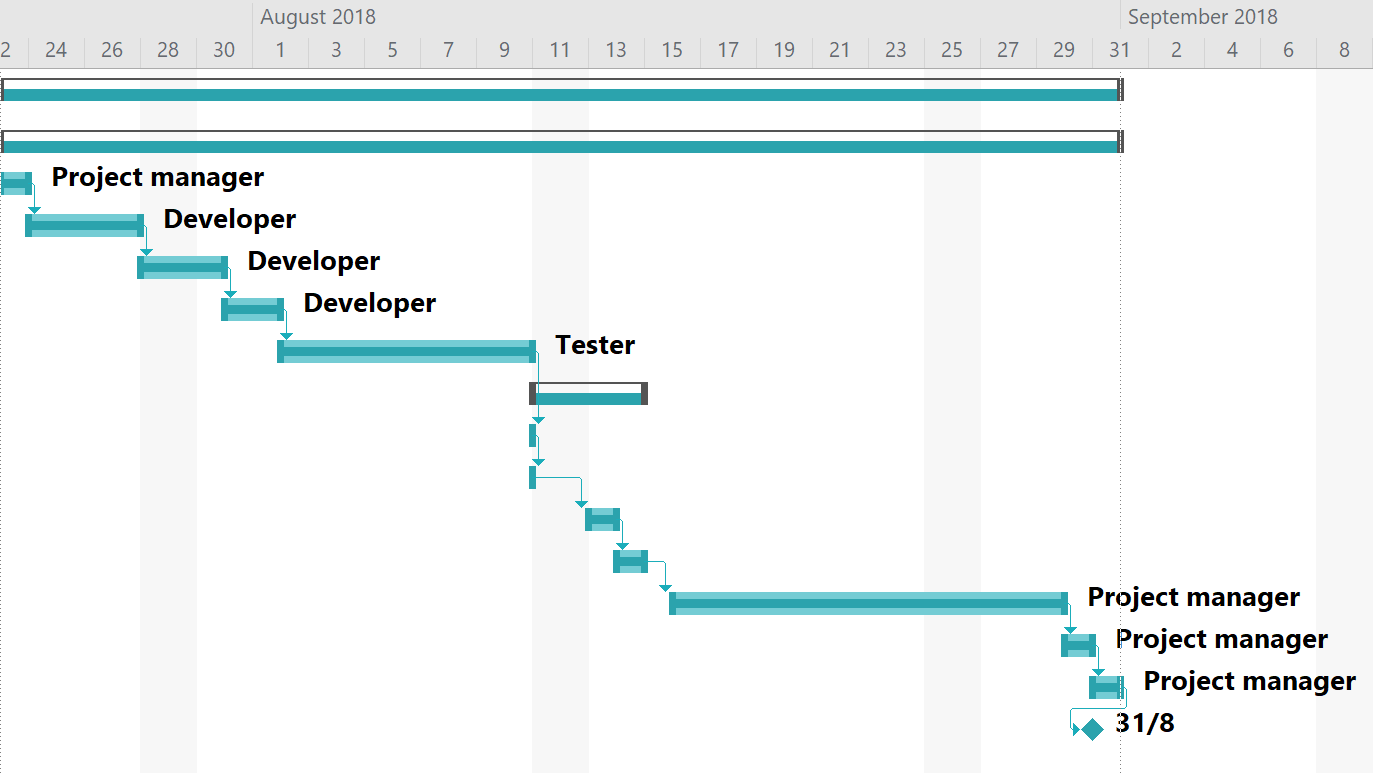
\includegraphics[width=17 cm,height=7cm]{Images/planning/iterations/It5_gantt} \\
				\label{fig:planning-it5-gantt} 
			\end{center}  
		\end{figure}  
		
	\end{itemize}
	
	% New page
	\newpage
	
	% Section
	\section{Estimación de costes}
		
	Otro aspecto importante a la hora de planificar y gestionar un proyecto es la elaboración de una estimación de costes totales que puede suponer el desarrollo de éste. En un proyecto real con uno o varios clientes y equipos de trabajo, la definición de estos costes debe aproximarse lo máximo posible a la realidad necesitada ya que puede conllevar al éxito o fracaso del proyecto. Estos costes a estimar incluyen tanto el coste de los recursos humanos involucrados (responsable del proyecto, equipo de desarrollo, equipo de aseguramiento de la calidad (\textit{Quality Assurance} -QA-), analistas, diseñadores, etc.) como de herramientas \textit{hardware} y \textit{software} así como los costes de infraestructura, instalaciones y servicios consumibles. \\
	
	Para realizar la estimación del coste de este proyecto se estimará como si se hubiera desarrollado profesionalmente a excepción de algunas salvedades citadas a continuación. En este caso, se va a suponer que determinados dispositivos \textit{hardware} mencionados en la sección \ref{tools}. \nameref{tools} han sido adquiridos para este proyecto con el fin de una estimación más realista y los costes de infraestructura e instalación se obvian por el carácter de este trabajo: \gls{tfm-a}. Con respecto a los servicios consumibles, se tendrán en cuenta los cuantificables de una manera directa y obviando aquellos como por ejemplo: electricidad, material de oficina, etc. El desglose de costes es el siguiente: \\
	
	% New page
	\newpage
	% Cost of human resources
	\begin{longtable}{|m{4cm}|m{4cm}|m{5cm}|m{4cm}|}
		\hline
			
		\multicolumn{4}{|>{\columncolor{Gainsboro}}c|}{\textsc{Coste de recursos humanos}}
		\\ \hline
		
		\multicolumn{1}{|c|}{\textbf{Rol}\footnote{Cada rol puede presentar días laborales en varias iteraciones. Por ejemplo, el rol ``Responsable del proyecto'' presenta 21 días en la fase de inicio (1 iteración) y el resto de días pertenecen a las sucesivas iteraciones.}} & \multicolumn{1}{p{2.5cm}|}{\textbf{Coste/hora (\euro)}} & \multicolumn{1}{c|}{\textbf{Cantidad (días $\times$ horas)}} & \multicolumn{1}{p{2.3cm}|}{\textbf{Coste total (\euro)}}
		\\ \hline
				
		\multicolumn{1}{|l|}{Responsable del proyecto} & \multicolumn{1}{c|}{40 \euro} & \multicolumn{1}{c|}{42 días $\times$ 4 horas} & \multicolumn{1}{c|}{6720 \euro} 
		\\ \hline
		
		\multicolumn{1}{|l|}{Analista} & \multicolumn{1}{c|}{35 \euro} & \multicolumn{1}{c|}{23 días $\times$ 4 horas} & \multicolumn{1}{c|}{3220 \euro} 
		\\ \hline
		
		\multicolumn{1}{|l|}{Diseñador} & \multicolumn{1}{c|}{30 \euro} & \multicolumn{1}{c|}{19 días $\times$ 4 horas} & \multicolumn{1}{c|}{2280 \euro} 
		\\ \hline
		
		\multicolumn{1}{|p{3.7cm}|}{Desarrollador} & \multicolumn{1}{c|}{25 \euro} & \multicolumn{1}{c|}{122 días $\times$ 4 horas} & \multicolumn{1}{c|}{12200 \euro} 
		\\ \hline
		
		\multicolumn{1}{|p{3.7cm}|}{Tester} & \multicolumn{1}{c|}{25 \euro} & \multicolumn{1}{c|}{16 días $\times$ 4 horas} & \multicolumn{1}{c|}{1600 \euro} 
		\\ \hline
		
		\multicolumn{3}{|l|}{\textbf{Coste total de recursos humanos}} & \multicolumn{1}{c|}{\textbf{26020 \euro}} 
		\\ \hline
					
		\caption{Estimación del coste de recursos humanos}
	\end{longtable}
	
	\hspace{1cm}
	\newline
	\newline
	
	% Cost of human resources in each phase
	\begin{longtable}{|m{4cm}|m{4cm}|m{4cm}|m{4cm}|}
		\hline
			
		\multicolumn{4}{|>{\columncolor{Gainsboro}}c|}{\textsc{Coste de recursos humanos en cada fase}} \\ \hline
		
		\multicolumn{1}{|c|}{\textbf{Fase}} & \multicolumn{1}{|c|}{\textbf{Recurso}} & \multicolumn{1}{|c|}{\textbf{Días laborales}} & \multicolumn{1}{|c|}{\textbf{Coste total (\euro)}} \\ \hline
		
		\multicolumn{1}{|c|}{\multirow{6}{*}{Inicio}} & \multicolumn{1}{|c|}{Responsable del proyecto} & \multicolumn{1}{|c|}{21 días} & \multicolumn{1}{|c|}{3360 \euro} \\ \cline{2-4}
		& \multicolumn{1}{|l|}{Analista} & \multicolumn{1}{|c|}{-} & \multicolumn{1}{|c|}{-} \\ \cline{2-4} 
		& \multicolumn{1}{|l|}{Diseñador} & \multicolumn{1}{|c|}{-} & \multicolumn{1}{|c|}{-} \\ \cline{2-4} 
		& \multicolumn{1}{|l|}{Desarrollador} & \multicolumn{1}{|c|}{-} & \multicolumn{1}{|c|}{-} \\ \cline{2-4} 
		& \multicolumn{1}{|l|}{Tester} & \multicolumn{1}{|c|}{-} & \multicolumn{1}{|c|}{-} \\ \cline{2-4} 
		& \multicolumn{2}{|l|}{} & \multicolumn{1}{|c|}{\textbf{3360 \euro}} \\ \Cline{1pt}{1-4}
		
		\multicolumn{1}{|c|}{\multirow{6}{*}{Elaboración}} & \multicolumn{1}{|c|}{Responsable del proyecto} & \multicolumn{1}{|c|}{2 días} & \multicolumn{1}{|c|}{320 \euro} \\ \cline{2-4}
		& \multicolumn{1}{|l|}{Analista} & \multicolumn{1}{|c|}{17 días} & \multicolumn{1}{|c|}{2380 \euro} \\ \cline{2-4} 
		& \multicolumn{1}{|l|}{Diseñador} & \multicolumn{1}{|c|}{15 días} & \multicolumn{1}{|c|}{1800 \euro} \\ \cline{2-4} 
		& \multicolumn{1}{|l|}{Desarrollador} & \multicolumn{1}{|c|}{-} & \multicolumn{1}{|c|}{-} \\ \cline{2-4} 
		& \multicolumn{1}{|l|}{Tester} & \multicolumn{1}{|c|}{-} & \multicolumn{1}{|c|}{-} \\ \cline{2-4} 
		& \multicolumn{2}{|l|}{} & \multicolumn{1}{|c|}{\textbf{4500 \euro}} \\ \Cline{1pt}{1-4}
		
		\multicolumn{1}{|c|}{\multirow{6}{*}{Construcción - 1ª iteración}} & \multicolumn{1}{|c|}{Responsable del proyecto} & \multicolumn{1}{|c|}{2 días} & \multicolumn{1}{|c|}{320 \euro} \\ \cline{2-4}
		& \multicolumn{1}{|l|}{Analista} & \multicolumn{1}{|c|}{6 días} & \multicolumn{1}{|c|}{840 \euro} \\ \cline{2-4} 
		& \multicolumn{1}{|l|}{Diseñador} & \multicolumn{1}{|c|}{4 días} & \multicolumn{1}{|c|}{480 \euro} \\ \cline{2-4} 
		& \multicolumn{1}{|l|}{Desarrollador} & \multicolumn{1}{|c|}{52 días} & \multicolumn{1}{|c|}{5200 \euro} \\ \cline{2-4} 
		& \multicolumn{1}{|l|}{Tester} & \multicolumn{1}{|c|}{4 días} & \multicolumn{1}{|c|}{400 \euro} \\ \cline{2-4} 
		& \multicolumn{2}{|l|}{} & \multicolumn{1}{|c|}{\textbf{7240 \euro}} \\ \Cline{1pt}{1-4}
		
		\multicolumn{1}{|c|}{\multirow{6}{*}{Construcción - 2ª iteración}} & \multicolumn{1}{|c|}{Responsable del proyecto} & \multicolumn{1}{|c|}{2 días} & \multicolumn{1}{|c|}{320 \euro} \\ \cline{2-4}
		& \multicolumn{1}{|l|}{Analista} & \multicolumn{1}{|c|}{-} & \multicolumn{1}{|c|}{-} \\ \cline{2-4} 
		& \multicolumn{1}{|l|}{Diseñador} & \multicolumn{1}{|c|}{-} & \multicolumn{1}{|c|}{-} \\ \cline{2-4} 
		& \multicolumn{1}{|l|}{Desarrollador} & \multicolumn{1}{|c|}{59 días} & \multicolumn{1}{|c|}{5900 \euro} \\ \cline{2-4} 
		& \multicolumn{1}{|l|}{Tester} & \multicolumn{1}{|c|}{4 dias} & \multicolumn{1}{|c|}{400 \euro} \\ \cline{2-4} 
		& \multicolumn{2}{|l|}{} & \multicolumn{1}{|c|}{\textbf{6620 \euro}} \\ \Cline{1pt}{1-4}
		
		\multicolumn{1}{|c|}{\multirow{6}{*}{Transición}} & \multicolumn{1}{|c|}{Responsable del proyecto} & \multicolumn{1}{|c|}{15 días} & \multicolumn{1}{|c|}{2400 \euro} \\ \cline{2-4}
		& \multicolumn{1}{|l|}{Analista} & \multicolumn{1}{|c|}{-} & \multicolumn{1}{|c|}{-} \\ \cline{2-4} 
		& \multicolumn{1}{|l|}{Diseñador} & \multicolumn{1}{|c|}{-} & \multicolumn{1}{|c|}{-} \\ \cline{2-4} 
		& \multicolumn{1}{|l|}{Desarrollador} & \multicolumn{1}{|c|}{11 días} & \multicolumn{1}{|c|}{1100 \euro} \\ \cline{2-4} 
		& \multicolumn{1}{|l|}{Tester} & \multicolumn{1}{|c|}{8 días} & \multicolumn{1}{|c|}{800 \euro} \\ \cline{2-4} 
		& \multicolumn{2}{|l|}{} & \multicolumn{1}{|c|}{\textbf{4300 \euro}} \\ \Cline{1pt}{1-4}
		
		\multicolumn{3}{|l|}{\textbf{Coste total de recursos humanos}} & \multicolumn{1}{c|}{\textbf{26020 \euro}} 
		\\ \hline
					
		\caption{Estimación del coste de recursos humanos por fase}
	\end{longtable}
	
	\hspace{1cm}
	\newline
	
	% Cost of hardware
	\begin{longtable}{|m{4cm}|m{4cm}|m{4cm}|m{4cm}|}
		\hline
			
		\multicolumn{4}{|>{\columncolor{Gainsboro}}c|}{\textsc{Coste de hardware}}
		\\ \hline
		
		\multicolumn{1}{|c|}{\textbf{Dispositivo}} & \multicolumn{1}{c|}{\textbf{Coste unitario (\euro)}} & \multicolumn{1}{c|}{\textbf{Cantidad (Unidades)}} & \multicolumn{1}{c|}{\textbf{Coste total (\euro)}}
		\\ \hline
				
		\multicolumn{1}{|l|}{DELL U2713H} & \multicolumn{1}{c|}{509 \euro} & \multicolumn{1}{c|}{1ud} & \multicolumn{1}{c|}{509 \euro} 
		\\ \hline
				
		\multicolumn{1}{|l|}{Macbook Pro Mid 2014} & \multicolumn{1}{c|}{1000 \euro} & \multicolumn{1}{c|}{1ud} & \multicolumn{1}{c|}{1000 \euro} 
		\\ \hline
		
		\multicolumn{1}{|l|}{Magic Mouse 1} & \multicolumn{1}{c|}{79 \euro} & \multicolumn{1}{c|}{1ud} & \multicolumn{1}{c|}{79 \euro} 
		\\ \hline
		
		\multicolumn{1}{|p{5cm}|}{\gls{raspberry-a} 3 Starter Kit} & \multicolumn{1}{c|}{151.37 \euro} & \multicolumn{1}{c|}{1ud} & \multicolumn{1}{c|}{151.37 \euro} 
		\\ \hline
		
		\multicolumn{1}{|p{5cm}|}{\gls{raspberry-a} Cooling Kit} & \multicolumn{1}{c|}{4.56 \euro} & \multicolumn{1}{c|}{1ud} & \multicolumn{1}{c|}{4.56 \euro} 
		\\ \hline
		
		\multicolumn{1}{|p{5cm}|}{Kuman Starter Kit} & \multicolumn{1}{c|}{39.99 \euro} & \multicolumn{1}{c|}{1ud} & \multicolumn{1}{c|}{39.99 \euro} 
		\\ \hline
		
		\multicolumn{1}{|p{5cm}|}{\gls{raspberry-a} Camera Module V2 8MP} & \multicolumn{1}{c|}{17.65 \euro} & \multicolumn{1}{c|}{1ud} & \multicolumn{1}{c|}{17.65 \euro} 
		\\ \hline
		
		\multicolumn{1}{|p{5cm}|}{\Gls{breadboard}, placa de expansión y cableado} & \multicolumn{1}{c|}{8.96 \euro} & \multicolumn{1}{c|}{1ud} & \multicolumn{1}{c|}{8.96 \euro} 
		\\ \hline
		
		\multicolumn{1}{|p{5cm}|}{\gls{lcd-a} 16 $\times$ 2} & \multicolumn{1}{c|}{3,95 \euro} & \multicolumn{1}{c|}{1ud} & \multicolumn{1}{c|}{3,95 \euro} 
		\\ \hline
		
		\multicolumn{1}{|p{5cm}|}{\Gls{sensor} HC-SR04} & \multicolumn{1}{c|}{1.50 \euro} & \multicolumn{1}{c|}{1ud} & \multicolumn{1}{c|}{1.50 \euro} 
		\\ \hline
		
		\multicolumn{3}{|l|}{\textbf{Coste total de \textit{hardware}}} & \multicolumn{1}{c|}{\textbf{1815.98 \euro}} 
		\\ \hline
							
		\caption{Estimación del coste de hardware}
	\end{longtable}
	
	% New page
	\newpage
	
	% Cost of software
	\begin{longtable}{|m{4cm}|m{4cm}|m{4cm}|m{4cm}|}
		\hline
			
		\multicolumn{4}{|>{\columncolor{Gainsboro}}c|}{\textsc{Coste de software}}
		\\ \hline
		
		\multicolumn{1}{|c|}{\textbf{Herramienta}} & \multicolumn{1}{c|}{\textbf{Coste unitario (\euro)}} & \multicolumn{1}{c|}{\textbf{Cantidad (Unidades)}} & \multicolumn{1}{c|}{\textbf{Coste total (\euro)}}
		\\ \hline
		
		\multicolumn{1}{|l|}{Texpad} & \multicolumn{1}{c|}{24.99 \euro} & \multicolumn{1}{c|}{1ud} & \multicolumn{1}{c|}{24.99 \euro} \\ \hline
		
		\multicolumn{1}{|l|}{Resto de herramientas\color{red}*\footnote{Todo el \textit{software} utilizado ha sido el mencionado en la sección \ref{tools}. \nameref{tools}. Su licencia ha sido obtenida gratuitamente por ser estudiante, por ser \textit{software} libre o bien se ha utilizado la versión gratuita.}} & \multicolumn{1}{c|}{0 \euro} & \multicolumn{1}{c|}{1ud} & \multicolumn{1}{c|}{0 \euro} 
		\\ \hline
			
		\multicolumn{3}{|l|}{\textbf{Coste total de \textit{software}}} & \multicolumn{1}{c|}{\textbf{24.99 \euro}} 
		\\ \hline
					
		\caption{Estimación del coste de software}
	\end{longtable}
	
	% Cost of services
	\begin{longtable}{|m{4cm}|m{4cm}|m{4cm}|m{4cm}|}
		\hline
			
		\multicolumn{4}{|>{\columncolor{Gainsboro}}c|}{\textsc{Coste de servicios consumibles}}
		\\ \hline
		
		\multicolumn{1}{|c|}{\textbf{Servicios}} & \multicolumn{1}{c|}{\textbf{Coste unitario (\euro)}} & \multicolumn{1}{c|}{\textbf{Cantidad (Unidades)}} & \multicolumn{1}{c|}{\textbf{Coste total (\euro)}}
		\\ \hline
				
		\multicolumn{1}{|l|}{Conexión a Internet} & \multicolumn{1}{c|}{40 \euro /mes x 7 meses} & \multicolumn{1}{c|}{1ud} & \multicolumn{1}{c|}{280 \euro} 
		\\ \hline
				
		\multicolumn{3}{|l|}{\textbf{Coste total de servicios consumibles}} & \multicolumn{1}{c|}{\textbf{280 \euro}} 
		\\ \hline
					
		\caption{Estimación del coste de servicios consumibles}
	\end{longtable}
	
	% Total cost
	\begin{longtable}{|m{5cm}|m{5cm}|}
		\hline
			
		\multicolumn{2}{|>{\columncolor{Gainsboro}}c|}{\textsc{Coste total del proyecto}}
		\\ \hline
		
		\multicolumn{1}{|c|}{\textbf{Apartado}} & \multicolumn{1}{c|}{\textbf{Coste total (\euro)}} 
		\\ \hline
				
		\multicolumn{1}{|l|}{Recursos humanos} & \multicolumn{1}{c|}{26020 \euro}
		\\ \hline
		
		\multicolumn{1}{|l|}{Hardware} & \multicolumn{1}{c|}{1815.98 \euro}
		\\ \hline
		
		\multicolumn{1}{|l|}{Software} & \multicolumn{1}{c|}{24.99 \euro}
		\\ \hline
		
		\multicolumn{1}{|l|}{Servicios consumibles} & \multicolumn{1}{c|}{280 \euro}
		\\ \hline
		
		\multicolumn{1}{|p{3.5cm}|}{\textbf{Total proyecto}} & \multicolumn{1}{c|}{\textbf{28140.97 \euro}} 
		\\ \hline
					
		\caption{Estimación del coste total del proyecto}
	\end{longtable}
	
	Por tanto, el presupuesto total estimado para la ejecución material del proyecto, asciende a la cantidad de {28140.97 \euro}.
	
	% Section
	\section{Gestión de riesgos}
	
	Se define \textit{riesgo} como la probabilidad de que un problema potencial, circunstancia o eventualidad adversa al proyecto y/o al entorno de éste ocurra en el tiempo, imposibilitando la consecución de un objetivo y las consecuencias que puede conllevar si finalmente se materializa. La gestión de riesgos \cite{incibe:GR} por su parte, es la práctica de valorar y controlar los riesgos que afectan a un producto, proceso o proyecto \textit{software} con el objetivo de poder anticiparse a los mismos antes de que éstos ocurran. La gestión del riesgo es necesaria debido a que:
	
	\begin{itemize}
		\item El riesgo del \textit{software} es inherente en este ámbito.
		\item El riesgo aumenta a medida que aumenta la complejidad del sistema.
		\item El riesgo impide conseguir los objetivos si no se considera.
		\item El riesgo tiene su máximo valor al comienzo de un proyecto.
		\item El coste de reacción ante un riesgo es mayor a medida que el proyecto avanza.
	\end{itemize}
	
	Por todas las razones comentadas anteriormente, hoy en día se hace inviable no disponer de una gestión de riesgos. En la siguiente imagen (Figura \ref{fig:plannig-cost-risk}), se puede observar lo necesario y fundamental que es una buena gestión de riesgos desde el comienzo del proyecto con el fin de anticiparse a ellos y así asegurar con mayor probabilidad el éxito y calidad de un proyecto sin perjudicar gravemente en la planificación y/o en la estimación de costes. \\

	\begin{figure}[!ht]   
		\caption{Relación coste-riesgo.} 
		\begin{center} 
	 		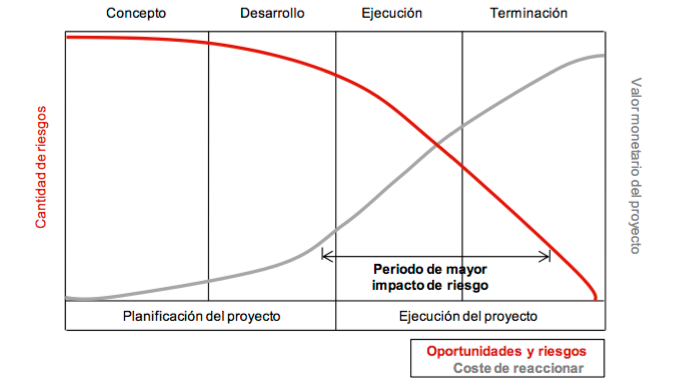
\includegraphics[width=16cm,height=7cm]{Images/planning/cost_risk} \\
			\label{fig:plannig-cost-risk} 
			Referencia bibliográfica: \cite{incibe:GAGR}
		\end{center}  
	\end{figure}  
		
	% Subsection
	\subsection{Identificación y análisis de riesgos}
	
	El propósito de esta sección es, en primer lugar, identificar y realizar un análisis de los posibles riesgos que se puedan producir y en segundo lugar, establecer unas pautas de monitorización de los mismos por medio de la definición de un plan de acción para cada uno de ellos con el fin de que se puedan gestionar en caso de ocurrencia. Antes de listar los riesgos identificados, se expone la tipología principal de categorización que se ha seguido:
	
	\begin{itemize}
		\item Riesgo de proyecto: relacionado con las restricciones de recursos y relaciones externas necesarias para la realización del proyecto.
		\item Riesgo de proceso: relacionado con la consecución y revisión de cada una de las fases de desarrollo del proyecto.
		\item Riesgo de producto: relacionado con la experiencia en el dominio y con los resultados ineficientes en las fases previas al desarrollo.
	\end{itemize}
	
	Otro catalogación es aquella donde se clasifican en función de los siguientes dos conceptos:
	
	\begin{itemize}
		\item Impacto: mide el grado de fracaso y degradación del objetivo si se produce el riesgo.
		\item Probabilidad: mide la posibilidad de ocurrencia de un riesgo.
	\end{itemize}
		
	A continuación, se describen los principales riesgos detectados ordenados de mayor a menor según su exposición donde se considera \textbf{Riesgo = Probabilidad de amenaza $\times$ Magnitud de daño} y su valoración ha sido calculada según la norma estándar \gls{iso27005}\footnote{Norma perteneciente a la familia ISO/IEC 27000. Consultar \cite{iso2013} para obtener más información.} (Figura \ref{fig:planning-risk-standard}).
	
	\begin{figure}[!ht]   
		\caption{Estándar de gestión de riesgos ISO/IEC 27005:2008.} 
		\begin{center} 
	 		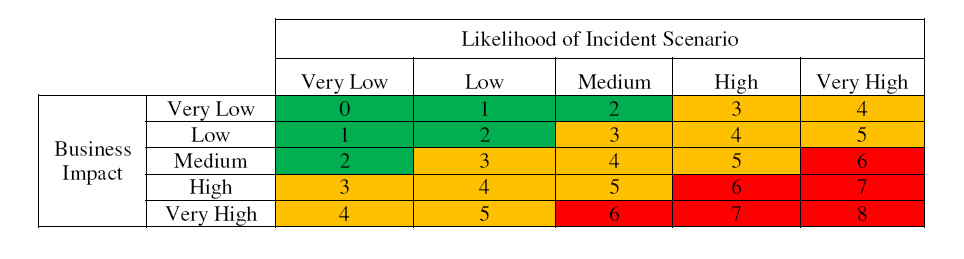
\includegraphics[width=16cm,height=5cm]{Images/planning/ISO7005} \\
			\label{fig:planning-risk-standard} 
			Referencia bibliográfica: \cite{risk:MMPQRM}
		\end{center}  
	\end{figure}  
					
	% New page
	\newpage
					
	% Planificación temporal errónea
	\begin{longtable}{m{4cm}|m{5cm}|m{4cm}}
		\hline
		\multicolumn{3}{|>{\columncolor{Gainsboro}}c|}{\multirow{1}{*}{\textsc{\large Formulario de gestión de riesgos}}}                                                         \\ \hline
		
		\multicolumn{1}{|>{\columncolor{Gainsboro}}c|}{\textbf{Identificador:} 1} & \multicolumn{1}{m{3.5cm}|}{Fecha: 29/12/2017}  & \multicolumn{1}{|m{8cm}|}{Fase: En todas las fases} \\ \hline
				
		\multicolumn{2}{|l|}{Título: \textbf{Planificación temporal errónea}} & \multicolumn{1}{|p{8cm}|}{Categoría: Riesgo de proyecto} \\ \hline
				
		\multicolumn{1}{|p{4cm}|}{Impacto: Muy alto} & \multicolumn{1}{|p{4cm}|}{Probabilidad: Media}  & \multicolumn{1}{|p{4.5cm}|}{Exposición: {\color{red}6} (Fig. \ref{fig:planning-risk-standard})}  \\ \hline
				
		\multicolumn{3}{|p{17cm}|}{Consecuencia: Retraso en el desarrollo del proyecto pudiendo derivar a una finalización tardía lo que supondría la cancelación del proyecto o insatisfacción por parte del cliente.}            \\ \hline \hline
				
		\multicolumn{3}{|c|}{\textbf{Valoración de riesgos}}    \\ \hline \hline
		\multicolumn{3}{|p{17cm}|}{Descripción del riesgo: La planificación inicial no ha sido realizada de forma asumible y por tanto la duración de los plazos establecidos son irreales y no se pueden cumplir.} \\ \hline
		\multicolumn{3}{|p{17cm}|}{Contexto del riesgo: Realizar durante la fase de inicio del proyecto una planificación inadecuada, ya sea por inexperiencia del responsable u otros motivos, puede provocar una asignación temporal completa que sea incorrecta y poco fiable.} \\ \hline
		\multicolumn{3}{|p{17cm}|}{Análisis del riesgo: La planificación inicial es uno de los puntos donde se precisa de la máxima exactitud para alcanzar el éxito del proyecto. En la situación actual, existe una probabilidad media de que se produzca una planificación que posteriormente no se pueda cumplir. El impacto, en este caso es muy alto debido a que el proyecto debe estar finalizado antes de la fecha de entrega por lo que no se admite un posible retraso y es crucial realizar una estimación temporal lo más realista posible.}  \\ \hline \hline
				
		\multicolumn{3}{|c|}{\textbf{Planificación de riesgos}} \\ \hline \hline
		\multicolumn{3}{|p{17cm}|}{Estrategia: Protección del riesgo.} \\ \hline
		\multicolumn{3}{|p{17cm}|}{Plan de contingencia preventivo: En la fase de inicio, tomar decisiones de planificación con la máxima exactitud a través del análisis en profundidad de los requerimientos del proyecto y ampliar los márgenes de error ante posibles fallos de planificación.} \\ \hline
		\multicolumn{3}{|p{17cm}|}{Plan de contingencia mitigante: Efectuar una nueva planificación del proyecto restante de forma instantánea, asignando en el caso más extremo más carga de trabajo diaria para así poder cumplir los plazos establecidos.} \\ \hline
				
		\multicolumn{3}{|c|}{\textbf{Punto de ruptura}} \\ \hline \hline
		\multicolumn{3}{|p{17cm}|}{Si se alcanza un retraso mayor al 40\% sobre la planificación inicial, no existirá un método de recuperar el trabajo demorado ya que la única forma sería mediante la asignación de una carga mayor de trabajo lo cual no es asumible debido a la limitación de la existencia de un solo recurso para el desarrollo del proyecto. Por tanto, el proyecto no podrá ser entregado en el plazo establecido para ello.}\\ \hline
				
		\multicolumn{3}{|c|}{\textbf{Resolución del riesgo}} \\ \hline \hline
		\multicolumn{3}{|p{17cm}|}{Responsable: Jesús Iglesias García}\\ \hline
		\multicolumn{3}{|p{17cm}|}{Rol: Responsable del proyecto} \\ \hline
		\caption{Riesgo 1 - Planificación temporal errónea}
	\end{longtable}
	
	\hspace{1cm}
			
	% Análisis del sistema inadecuado
	\begin{longtable}{m{4cm}|m{5cm}|m{4cm}}
		\hline
		\multicolumn{3}{|>{\columncolor{Gainsboro}}c|}{\multirow{1}{*}{\textsc{\large Formulario de gestión de riesgos}}}                                                         \\ \hline
	
		\multicolumn{1}{|>{\columncolor{Gainsboro}}c|}{\textbf{Identificador:} 2} & \multicolumn{1}{m{3.5cm}|}{Fecha: 29/12/2017}  & \multicolumn{1}{|m{8cm}|}{Fase: Elaboración} \\ \hline
			
		\multicolumn{2}{|l|}{Título: \textbf{Análisis del sistema inadecuado}} &\multicolumn{1}{|p{8cm}|}{Categoría: Riesgo de proceso} \\ \hline
			
		\multicolumn{1}{|p{4cm}|}{Impacto: Alto} & \multicolumn{1}{|p{4cm}|}{Probabilidad: Baja}  & \multicolumn{1}{|p{4.5cm}|}{Exposición: {\color{amber}4} (Fig. \ref{fig:planning-risk-standard})}  \\ \hline
			
		\multicolumn{3}{|p{17cm}|}{Consecuencia: Sistema implementado sin satisfacer los requerimientos y funcionalidades previamente establecidas.} \\ \hline \hline
			
		\multicolumn{3}{|c|}{\textbf{Valoración de riesgos}}    \\ \hline \hline
		\multicolumn{3}{|p{17cm}|}{Descripción del riesgo: Gestión pobre durante la etapa de análisis del sistema, ya sea por una extracción de requisitos incorrecta o incompleta.} \\ \hline
		\multicolumn{3}{|p{17cm}|}{Contexto del riesgo: Solamente un recurso humano a tiempo parcial se va a dedicar al análisis del sistema por lo que no es del todo posible establecer una organización y trabajo en equipo lo cual proporcionaría en gran medida un mejor análisis. Es por ello que este recurso es el encargado de la decisión y si no posee demasiada experiencia o el proyecto no se encuentra bien definido, puede proporcionar un planteamiento erróneo.} \\ \hline
		\multicolumn{3}{|p{17cm}|}{Análisis del riesgo: Cuando se inicia un nuevo proyecto, la asignación de recursos humanos se hace en base a obtener el máximo rendimiento y calidad final del producto/servicio por lo que se asignan en la medida de lo posible recursos con experiencia en cada fase. En este caso debido a la naturaleza del proyecto, se ha asignado a un analista a tiempo parcial para efectuar el análisis de un sistema que se encuentra bien definido por lo que la probabilidad de riesgo es baja y su impacto se considera alto ya que afectaría de forma negativa al desarrollo normal del proyecto, repercutiendo a su vez en una posible reestructuración del proyecto entero y por tanto afectando a la planificación.}  \\ \hline \hline
			
		\multicolumn{3}{|c|}{\textbf{Planificación de riesgos}} \\ \hline \hline
		\multicolumn{3}{|p{17cm}|}{Estrategia: Protección del riesgo.} \\ \hline
		\multicolumn{3}{|p{17cm}|}{Plan de contingencia preventivo: Concretar revisiones de los requisitos para refinarlos durante la primera iteración de la fase de construcción.} \\ \hline
		\multicolumn{3}{|p{17cm}|}{Plan de contingencia mitigante: Mejorar la definición del proyecto y analizar detenidamente el sistema de nuevo cuando surjan los primeros indicios de un desarrollo incompleto o incorrecto.} \\ \hline
			
		\multicolumn{3}{|c|}{\textbf{Punto de ruptura}} \\ \hline \hline
		\multicolumn{3}{|p{17cm}|}{Si durante la mitad de la segunda iteración de la fase de construcción, los requisitos y funcionalidades se manifiestan como incompletos o erróneos y suponen un 30\% del total del sistema a construir, el proyecto se considera como no asumible al no cumplir con los plazos establecidos.}\\ \hline
			
		\multicolumn{3}{|c|}{\textbf{Resolución del riesgo}} \\ \hline \hline
		\multicolumn{3}{|p{17cm}|}{Responsable: Jesús Iglesias García}\\ \hline
		\multicolumn{3}{|p{17cm}|}{Rol: Analista del proyecto} \\ \hline
		\caption{Riesgo 2 - Análisis del sistema inadecuado}
	\end{longtable}
	
	\hspace{1cm}
	
	% Diseño del sistema inadecuado
	\begin{longtable}{m{4cm}|m{5cm}|m{4cm}}
		\hline
		\multicolumn{3}{|>{\columncolor{Gainsboro}}c|}{\multirow{1}{*}{\textsc{\large Formulario de gestión de riesgos}}}                                                         \\ \hline
	
		\multicolumn{1}{|>{\columncolor{Gainsboro}}c|}{\textbf{Identificador:} 3} & \multicolumn{1}{m{3.5cm}|}{Fecha: 29/12/2017}  & \multicolumn{1}{|m{8cm}|}{Fase: Elaboración} \\ \hline
			
		\multicolumn{2}{|l|}{Título: \textbf{Diseño del sistema inadecuado}} & \multicolumn{1}{|p{8cm}|}{Categoría: Riesgo de proceso} \\ \hline
			
		\multicolumn{1}{|p{4cm}|}{Impacto: Alto} & \multicolumn{1}{|p{4cm}|}{Probabilidad: Baja}  & \multicolumn{1}{|p{4.5cm}|}{Exposición: {\color{amber}4} (Fig. \ref{fig:planning-risk-standard})}  \\ \hline
			
		\multicolumn{3}{|p{17cm}|}{Consecuencia: Sistema implementado sin satisfacer la arquitectura física previamente establecida.} \\ \hline \hline
			
		\multicolumn{3}{|c|}{\textbf{Valoración de riesgos}}    \\ \hline \hline
		\multicolumn{3}{|p{17cm}|}{Descripción del riesgo: Gestión pobre durante la etapa de diseño del sistema, ya sea por un modelado de la arquitectura física del sistema incorrecta o incompleta.} \\ \hline
		\multicolumn{3}{|p{17cm}|}{Contexto del riesgo: Solamente un recurso humano a tiempo parcial se va a dedicar al diseño por lo que es esencial que conozca profundamente la definición del proyecto y el análisis previamente realizado sobre éste y en base a estos dos aspectos encargarse de la decisión. Por lo que si no posee demasiada experiencia o el proyecto no se encuentra bien definido, puede plantear una arquitectura errónea.} \\ \hline
		\multicolumn{3}{|p{17cm}|}{Análisis del riesgo: En este caso debido a la naturaleza del proyecto, tanto éste como su análisis se encuentran bien definidos por lo que la probabilidad de un diseño erróneo es baja. Su impacto se considera alto ya que afectaría de forma negativa al desarrollo normal del proyecto, repercutiendo a su vez en una posible reestructuración del proyecto entero y por tanto afectando a la planificación.}  \\ \hline \hline			
			
		\multicolumn{3}{|c|}{\textbf{Planificación de riesgos}} \\ \hline \hline
		\multicolumn{3}{|p{17cm}|}{Estrategia: Protección del riesgo.} \\ \hline
		\multicolumn{3}{|p{17cm}|}{Plan de contingencia preventivo: Concretar varias revisiones del modelado físico de la arquitectura al comienzo de la primera iteración de la fase de construcción.} \\ \hline
		\multicolumn{3}{|p{17cm}|}{Plan de contingencia mitigante: Analizar la arquitectura actual y las posibles variantes a adoptar cuando surjan los primeros indicios de un diseño inestable.} \\ \hline
						
		\multicolumn{3}{|c|}{\textbf{Punto de ruptura}} \\ \hline \hline
		\multicolumn{3}{|p{17cm}|}{Si al comienzo de la segunda iteración de la fase de construcción, el modelado de la arquitectura física se considera incompleto o erróneo y supone una reestructuración de al menos el 50\% del sistema a construir, el proyecto se considera como no asumible al no cumplir con los plazos establecidos.}\\ \hline
			
		\multicolumn{3}{|c|}{\textbf{Resolución del riesgo}} \\ \hline \hline
		\multicolumn{3}{|p{17cm}|}{Responsable: Jesús Iglesias García}\\ \hline
		\multicolumn{3}{|p{17cm}|}{Rol: Diseñador del proyecto} \\ \hline
		\caption{Riesgo 3 - Diseño del sistema inadecuado}		
	\end{longtable}
	
	\hspace{1cm}
				
	% Falta de experiencia en la tecnología a utilizar
	\begin{longtable}{m{4cm}|m{5cm}|m{4cm}}
		\hline
		\multicolumn{3}{|>{\columncolor{Gainsboro}}c|}{\multirow{1}{*}{\textsc{\large Formulario de gestión de riesgos}}} \\ \hline
	
		\multicolumn{1}{|>{\columncolor{Gainsboro}}c|}{\textbf{Identificador:} 4} & \multicolumn{1}{m{3.5cm}|}{Fecha: 29/12/2017}  & \multicolumn{1}{|m{8cm}|}{Fase: Construcción y transición} \\ \hline
			
		\multicolumn{2}{|l|}{Título: \textbf{Inexperiencia con la tecnología}} & \multicolumn{1}{|p{8cm}|}{Categoría: Riesgo de producto} \\ \hline
			
		\multicolumn{1}{|p{4cm}|}{Impacto: Alto} & \multicolumn{1}{|p{4cm}|}{Probabilidad: Baja}  & \multicolumn{1}{|p{4.5cm}|}{Exposición: {\color{amber}4} (Fig. \ref{fig:planning-risk-standard})}  \\ \hline
			
		\multicolumn{3}{|p{17cm}|}{Consecuencia: El desconocimiento y falta de experiencia de la tecnología de desarrollo podría provocar un retraso en la planificación al tener que obtener formación o una implementación incorrecta o ineficiente.} \\ \hline \hline
			
		\multicolumn{3}{|c|}{\textbf{Valoración de riesgos}}    \\ \hline \hline
		\multicolumn{3}{|p{17cm}|}{Descripción del riesgo: Falta de conocimiento de los lenguajes de programación, \textit{\glspl{framework}} y librerías a utilizar para el desarrollo.} \\ \hline
		\multicolumn{3}{|p{17cm}|}{Contexto del riesgo: El desarrollador presenta experiencia en alguna de las tecnologías a utilizar mientras que en otras carece de ella. Si bien es cierto que existe documentación exhaustiva donde apoyarse, no se descarta que esta documentación en algunos casos sea escasa debido a que se tratan de tecnologías nuevas lo que podría convertirse en un contratiempo.} \\ \hline 
		\multicolumn{3}{|p{17cm}|}{Análisis del riesgo: Para desarrollar el proyecto se dispone en principio del conocimiento necesario para abordarlo sin ningún inconveniente sumado a la documentación detallada existente y con ejemplos. En principio, la probabilidad de ocurrencia de este riesgo es baja. Sin embargo, en caso de ocurrir se consideraría un grave problema ya que afectaría de manera directa a la realización del proyecto causando posibles retrasos siendo por este motivo su impacto alto.}  \\ \hline \hline
            	
		\multicolumn{3}{|c|}{\textbf{Planificación de riesgos}} \\ \hline \hline
		\multicolumn{3}{|p{17cm}|}{Estrategia principal: Protección del riesgo.} \\ \hline
		\multicolumn{3}{|p{17cm}|}{Plan de contingencia preventivo: Consultar referencias sobre aquellas tecnologías donde se presenten dudas, apoyándose en especial en la documentación oficial y sus ejemplos ya que facilitan el entendimiento de la estructura y funcionalidad del código a través de la exposición de la interfaz de programación (\textit{\gls{api}} -\gls{api-a}-).} \\ \hline
		\multicolumn{3}{|p{17cm}|}{Plan de contingencia mitigante: Establecer durante la primera iteración de la fase de desarrollo un marco temporal de aprendizaje sobre las tecnologías a utilizar. Esto sería posible gracias a la holgura existente en la planificación inicial.} \\ \hline
			
		\multicolumn{3}{|c|}{\textbf{Punto de ruptura}} \\ \hline \hline
		\multicolumn{3}{|p{17cm}|}{Si el desarrollador presenta problemas a la hora de codificar el sistema, no considerándose completamente funcional y produciéndose un retraso del 40\% con respecto a la planificación inicial, el proyecto se considera como no subsanable debido a la falta de tiempo y recursos para solucionar los errores presentados.}\\ \hline
			
		\multicolumn{3}{|c|}{Resolución del riesgo} \\ \hline \hline
		\multicolumn{3}{|p{17cm}|}{Responsable: Jesús Iglesias García}\\ \hline
		\multicolumn{3}{|p{17cm}|}{Rol: Desarrollador del proyecto} \\ \hline
		\caption{Riesgo 4 - Inexperiencia con la tecnología}
	\end{longtable}	
			
	% Ausencia de personal
	\begin{longtable}{m{4cm}|m{5cm}|m{4cm}}
		\hline
		\multicolumn{3}{|>{\columncolor{Gainsboro}}c|}{\multirow{1}{*}{\textsc{\large Formulario de gestión de riesgos}}}                                                         \\ \hline
						
		\multicolumn{1}{|>{\columncolor{Gainsboro}}c|}{\textbf{Identificador:} 5} & \multicolumn{1}{m{5.5cm}|}{Fecha: 29/12/2017}  & \multicolumn{1}{|m{6cm}|}{Fase: En todas las fases} \\ \hline
			
		\multicolumn{2}{|l|}{Título: \textbf{Ausencia de personal}} & \multicolumn{1}{|p{6cm}|}{Categoría: Riesgo de proyecto} \\ \hline
			
		\multicolumn{1}{|p{4cm}|}{Impacto: Muy alto} & \multicolumn{1}{|p{6cm}|}{Probabilidad: Muy baja}  & \multicolumn{1}{|p{4.5cm}|}{Exposición: {\color{amber}4} (Fig. \ref{fig:planning-risk-standard})}  \\ \hline
			
		\multicolumn{3}{|p{17cm}|}{Consecuencia: Retraso en la finalización del proyecto, no cumpliendo por tanto los plazos planificados inicialmente.} \\ \hline \hline
			
		\multicolumn{3}{|c|}{\textbf{Valoración de riesgos}}    \\ \hline \hline
		\multicolumn{3}{|p{17cm}|}{Descripción del riesgo: Imposibilidad de avanzar en el proyecto por causas de fuerza mayor ya sea por motivos internos o externos al proyecto, repercutiendo en el retraso de las entregas o en el aumento de la cantidad de trabajo para finalizar en el mismo instante de tiempo.} \\ \hline
		\multicolumn{3}{|p{17cm}|}{Contexto del riesgo: Está presente durante todo el ciclo de vida del proyecto ya que al ser un factor humano puede manifestarse en cualquier instante.} \\ \hline
		\multicolumn{3}{|p{17cm}|}{Análisis del riesgo: Este riesgo ha sido marcado con un valor de probabilidad muy bajo ya que aunque depende de factores variables y se puede dar en cualquier instante, no es una situación habitual que afecte de manera permanente al desarrollo del proyecto. Si que es verdad que posee un impacto muy alto ya que la ausencia continuada y en gran cantidad repercute negativamente al avance.}  \\ \hline \hline

		\multicolumn{3}{|c|}{\textbf{Planificación de riesgos}} \\ \hline \hline
		\multicolumn{3}{|p{17cm}|}{Estrategia principal: Reducción del riesgo} \\ \hline
		\multicolumn{3}{|p{17cm}|}{Plan de contingencia preventivo: Establecer márgenes temporales en la planificación para afrontar estos posibles sucesos de tal manera que no repercutan o que repercutan lo mínimo posible. Replanificar la carga de trabajo restante para finalizar en el mismo plazo.} \\ \hline
		\multicolumn{3}{|p{17cm}|}{Plan de contingencia mitigante: Replanificar la carga de trabajo y el marco temporal restante para adaptarse a los requisitos mínimos que debe contener la solución a implementar de forma que se incluyan más funcionalidades progresivamente si da tiempo.} \\ \hline
			
		\multicolumn{3}{|c|}{\textbf{Punto de ruptura}} \\ \hline \hline
		\multicolumn{3}{|p{17cm}|}{Si la ausencia de personal es elevada provocando severos retrasos con respecto a la planificación (40\%), la situación es irremediable y no se puede afrontar un reparto de la carga de trabajo restante ya que se consideraría excesivo. Debido a la naturaleza del proyecto, tampoco se dispone de otros recursos humanos que puedan continuar con el proyecto.}\\ \hline
			
		\multicolumn{3}{|c|}{\textbf{Resolución del riesgo}} \\ \hline \hline
		\multicolumn{3}{|p{17cm}|}{Responsable: Jesús Iglesias García}\\ \hline
		\multicolumn{3}{|p{17cm}|}{Rol: Responsable del proyecto} \\ \hline
		\caption{Riesgo 5 - Ausencia de personal}
	\end{longtable}
	
	% NEW PAGE
	\newpage
							
	% Bugs en implementación
	\begin{longtable}{m{4cm}|m{5cm}|m{4cm}}
		\hline
		\multicolumn{3}{|>{\columncolor{Gainsboro}}c|}{\multirow{1}{*}{\textsc{\large Formulario de gestión de riesgos}}}                                                         \\ \hline
	
		\multicolumn{1}{|>{\columncolor{Gainsboro}}c|}{\textbf{Identificador:} 6} & \multicolumn{1}{m{3.5cm}|}{Fecha: 29/12/2017}  & \multicolumn{1}{|m{8cm}|}{Fase: Construcción y transición} \\ \hline
			
		\multicolumn{2}{|l|}{Título: \textbf{\glspl{bug} en implementación}} & \multicolumn{1}{|p{8cm}|}{Categoría: Riesgo de producto} \\ \hline
			
		\multicolumn{1}{|p{4cm}|}{Impacto: Medio} & \multicolumn{1}{|p{4cm}|}{Probabilidad: Baja}  & \multicolumn{1}{|p{4.5cm}|}{Exposición: {\color{amber}3} (Fig. \ref{fig:planning-risk-standard})}  \\ \hline
			
		\multicolumn{3}{|p{17cm}|}{Consecuencia: Desarrollar un programa informático que presente errores de funcionalidad, diseño, seguridad, etc. supone que el tester notifique estos problemas al desarrollador y éste tenga que emplear tiempo y esfuerzo para su resolución lo cual a su vez implica la replanificación.} \\ \hline \hline
			
		\multicolumn{3}{|c|}{\textbf{Valoración de riesgos}}    \\ \hline \hline
		\multicolumn{3}{|p{17cm}|}{Descripción del riesgo: Una elevada complejidad algorítmica y de la solución puede suponer dificultad a la hora de codificar y por tanto desarrollar un sistema con funcionalidad incorrecta que no cumpla las necesidades requeridas.} \\ \hline
		\multicolumn{3}{|p{17cm}|}{Contexto del riesgo: El desarrollador debido al desconocimiento de las tecnologías puede cometer errores en la codificación o incluso estar debido a una especificación incorrecta de la solución.} \\ \hline
		\multicolumn{3}{|p{17cm}|}{Análisis del riesgo: Aunque en principio el análisis y diseño del proyecto están correctamente definidos puede que durante el transcurso del ciclo de vida de éste se realice alguna modificación que el desarrollador olvide implementar. Incluso puede ser el desarrollador el que rompa alguna funcionalidad anterior al incluir nuevas. Aun así se considera que tanto la probabilidad como su impacto sean medios debido a una detección temprana por el tester. Esto implicaría una notificación prematura, reduciendo así el riesgo con un muy leve retraso en la codificación de alguna tarea específica subsanable con el aumento de la carga en otro día laboral.}  \\ \hline \hline			
			            	
		\multicolumn{3}{|c|}{\textbf{Planificación de riesgos}} \\ \hline \hline
		\multicolumn{3}{|p{17cm}|}{Estrategia principal: Prevención del riesgo.} \\ \hline
			
		\multicolumn{3}{|p{17cm}|}{Plan de contingencia preventivo: Al finalizar cada iteración de la fase de desarrollo, efectuar una batería de pruebas tanto funcionales como técnicas con el fin de detectar lo antes posible cualquier error en la solución.} \\ \hline
		\multicolumn{3}{|p{17cm}|}{Plan de contingencia mitigante: Efectuar al finalizar la introducción de una nueva funcionalidad una batería de pruebas exhaustiva con lo que la detección de cualquier problema sería en su fase más temprana y su resolución no supondría un contratiempo grande en la planificación ni un retraso en el proyecto.} \\ \hline

		\multicolumn{3}{|c|}{\textbf{Punto de ruptura}} \\ \hline \hline
		\multicolumn{3}{|p{17cm}|}{Si se localizan demasiados fallos de funcionalidad y diseño durante la fase de transición y esta cifra alcanza un 40\% se considera que el tiempo necesario para revertir esta situación sobrepasaría la fecha límite de entrega o tendría un sobrecoste inasumible.}\\ \hline
				
		\multicolumn{3}{|c|}{Resolución del riesgo} \\ \hline \hline
		\multicolumn{3}{|p{17cm}|}{Responsable: Jesús Iglesias García}\\ \hline
		\multicolumn{3}{|p{17cm}|}{Rol: Desarrollador y tester del proyecto} \\ \hline
		\caption{Riesgo 6 - Bugs en la implementación}					
	\end{longtable}	
	
	\hspace{1cm}
				
	% Carencia de presupuesto
	\begin{longtable}{m{4cm}|m{5cm}|m{4cm}}
		\hline
		\multicolumn{3}{|>{\columncolor{Gainsboro}}c|}{\multirow{1}{*}{\textsc{\large Formulario de gestión de riesgos}}}                                                         \\ \hline
			
		\multicolumn{1}{|>{\columncolor{Gainsboro}}c|}{\textbf{Identificador:} 7} & \multicolumn{1}{m{5.5cm}|}{Fecha: 29/12/2017}  & \multicolumn{1}{|m{6cm}|}{Fase: En todas las fases} \\ \hline
			
		\multicolumn{2}{|l|}{Título: \textbf{Carencia de presupuesto}} & \multicolumn{1}{|p{6cm}|}{Categoría: Riesgo de proyecto} \\ \hline
			
		\multicolumn{1}{|p{4cm}|}{Impacto: Medio} & \multicolumn{1}{|p{6cm}|}{Probabilidad: Muy baja}  & \multicolumn{1}{|p{4.5cm}|}{Exposición: {\color{dartmouthgreen}2} (Fig. \ref{fig:planning-risk-standard})}  \\ \hline
			
		\multicolumn{3}{|p{17cm}|}{Consecuencia: No poder afrontar las actuales o nuevas necesidades del proyecto debido a la adquisición de recursos materiales provocaría retrasos en la planificación o no poder implementar todas las funcionalidades requeridas.} \\ \hline \hline
			
		\multicolumn{3}{|c|}{\textbf{Valoración de riesgos}}    \\ \hline \hline
		\multicolumn{3}{|p{17cm}|}{Descripción del riesgo: Aun habiendo adquirido todo el material necesario, puede existir en cualquier momento la inclusión de una nueva funcionalidad que necesite de un nuevo recurso material lo cual provoca costes económicos adicionales y pueden suponer no disponerlos, derivando en incompletitud de las funcionalidades del sistema.} \\ \hline
		\multicolumn{3}{|p{17cm}|}{Contexto del riesgo: Está presente durante todo el ciclo de vida del proyecto ya que constantemente se pueden requerir cambios que supongan costes adicionales a la estimación realizada en la planificación inicial.} \\ \hline
		\multicolumn{3}{|p{17cm}|}{Análisis del riesgo: La correcta definición del proyecto y por tanto también de los recursos materiales necesitados provocan que en principio no se necesite nada a mayores por lo que se determina que la probabilidad de este riesgo es muy baja y el impacto medio ya que podría darse el caso de no poder implementar una nueva funcionalidad al no poder adquirir el recurso material.}  \\ \hline \hline

		\multicolumn{3}{|c|}{\textbf{Planificación de riesgos}} \\ \hline \hline
		\multicolumn{3}{|p{17cm}|}{Estrategia principal: Protección del riesgo} \\ \hline			
		\multicolumn{3}{|p{17cm}|}{Plan de contingencia preventivo: Realizar durante la fase de inicio una estimación del coste global lo más aproximada posible, estudiando el proyecto con profundidad para conocer los recursos necesarios y así poder adaptarse al presupuesto existente.} \\ \hline
		\multicolumn{3}{|p{17cm}|}{Plan de contingencia mitigante: Reorganizar los recursos existentes para reducir en la medida de lo posible los inconvenientes que se puedan producir.} \\ \hline
			
		\multicolumn{3}{|c|}{\textbf{Punto de ruptura}} \\ \hline \hline
		\multicolumn{3}{|p{17cm}|}{Si la estimación de coste del nuevo material a adquirir supera el disponible no se puede aceptar dicha petición y por tanto no se puede implementar lo acordado.}\\ \hline
			
		\multicolumn{3}{|c|}{\textbf{Resolución del riesgo}} \\ \hline \hline
		\multicolumn{3}{|p{17cm}|}{Responsable: Jesús Iglesias García}\\ \hline
		\multicolumn{3}{|p{17cm}|}{Rol: Responsable del proyecto} \\ \hline
		\caption{Riesgo 7 - Carencia de presupuesto}			
	\end{longtable}
	
	\hspace{1cm}
	
	% Fallos de hardware
	\begin{longtable}{m{4cm}|m{5cm}|m{4cm}}
		\hline
		\multicolumn{3}{|>{\columncolor{Gainsboro}}c|}{\multirow{1}{*}{\textsc{\large Formulario de gestión de riesgos}}}                                                         \\ \hline
	
		\multicolumn{1}{|>{\columncolor{Gainsboro}}c|}{\textbf{Identificador:} 8} & \multicolumn{1}{m{3.5cm}|}{Fecha: 29/12/2017}  & \multicolumn{1}{|m{8cm}|}{Fase: En todas las fases} \\ \hline
			
		\multicolumn{2}{|l|}{Título: \textbf{Fallo de hardware}} & \multicolumn{1}{|p{8cm}|}{Categoría: Riesgo de producto} \\ \hline
			
		\multicolumn{1}{|p{4cm}|}{Impacto: Muy bajo} & \multicolumn{1}{|p{4cm}|}{Probabilidad: Baja}  & \multicolumn{1}{|p{4.5cm}|}{Exposición: {\color{dartmouthgreen}1} (Fig. \ref{fig:planning-risk-standard})}  \\ \hline
			
		\multicolumn{3}{|p{17cm}|}{Consecuencia: Retraso en las tareas del proyecto debido a la no disponibilidad de los recursos físicos necesarios para avanzar. También se pueden producir pérdidas de información importante.} \\ \hline \hline
			
		\multicolumn{3}{|c|}{\textbf{Valoración de riesgos}}    \\ \hline \hline
		\multicolumn{3}{|p{17cm}|}{Descripción del riesgo: Los dispositivos \textit{hardware} pueden averiarse o extraviarse durante el proyecto lo que afectaría al desarrollo normal de éste.} \\ \hline
		\multicolumn{3}{|p{17cm}|}{Contexto del riesgo: Está presente durante todo el proceso de desarrollo del proyecto ya que el mal funcionamiento o deterioro \textit{hardware} no es controlable directamente.} \\ \hline      
		\multicolumn{3}{|p{17cm}|}{Análisis del riesgo: Este riesgo se ha marcado con probabilidad baja debido a que el \textit{hardware} cada vez se construye con componentes más fiables y duraderos que no tienden al fallo. El impacto sería muy bajo ya que es muy común disponer de otros elementos \textit{hardware} como segunda opción siempre y cuando éstos no presenten un coste elevado. Para el proyecto actual, el \textit{hardware} necesitado es básico lo cual no implicaría un inconveniente a considerar si se produjese el fallo en alguno de ellos.}  \\ \hline \hline
           
		\multicolumn{3}{|c|}{\textbf{Planificación de riesgos}} \\ \hline \hline
		\multicolumn{3}{|p{17cm}|}{Estrategia principal: Aceptación del riesgo.} \\ \hline			
		\multicolumn{3}{|p{17cm}|}{Plan de contingencia preventivo: Realizar revisiones periódicas del estado de los sistemas \textit{hardware} y mantener estos sistemas en buena disposición.} \\ \hline
		\multicolumn{3}{|p{17cm}|}{Plan de contingencia mitigante: Disponer de dispositivos alternativos y copias de seguridad de la información importante para poder continuar el desarrollo del proyecto sin afectar gravemente a la planificación.} \\ \hline
			
		\multicolumn{3}{|c|}{\textbf{Punto de ruptura}} \\ \hline \hline
		\multicolumn{3}{|p{17cm}|}{Si el desarrollador durante la segunda iteración de la fase de construcción experimenta un fallo de \textit{hardware} perdiendo el código fuente del sistema por completo, se asume como no recuperable en el tiempo de planificación restante.}\\ \hline
					
		\multicolumn{3}{|c|}{\textbf{Resolución del riesgo}} \\ \hline \hline
		\multicolumn{3}{|p{17cm}|}{Responsable: Jesús Iglesias García}\\ \hline
		\multicolumn{3}{|p{17cm}|}{Rol: Responsable del proyecto} \\ \hline
		\caption{Riesgo 8 - Fallo de hardware}
	\end{longtable}
	
	% New page
	\newpage
	
	% Fallos de software.
	\begin{longtable}{m{4cm}|m{5cm}|m{4cm}}
		\hline
		\multicolumn{3}{|>{\columncolor{Gainsboro}}c|}{\multirow{1}{*}{\textsc{\large Formulario de gestión de riesgos}}}                                                         \\ \hline
				
		\multicolumn{1}{|>{\columncolor{Gainsboro}}c|}{\textbf{Identificador:} 9} & \multicolumn{1}{m{3.5cm}|}{Fecha: 29/12/2017}  & \multicolumn{1}{|m{8cm}|}{Fase: En todas las fases} \\ \hline
			
		\multicolumn{2}{|l|}{Título: \textbf{Fallo de software}} & \multicolumn{1}{|p{8cm}|}{Categoría: Riesgo de producto} \\ \hline
			
		\multicolumn{1}{|p{4cm}|}{Impacto: Muy bajo} & \multicolumn{1}{|p{4cm}|}{Probabilidad: Baja}  & \multicolumn{1}{|p{4.5cm}|}{Exposición: {\color{dartmouthgreen}1} (Fig. \ref{fig:planning-risk-standard})}  \\ \hline
			
		\multicolumn{3}{|p{17cm}|}{Consecuencia: Retraso en el avance del proyecto y/o pérdidas de información importante.} \\ \hline \hline
			
		\multicolumn{3}{|c|}{\textbf{Valoración de riesgos}}    \\ \hline \hline
		\multicolumn{3}{|p{17cm}|}{Descripción del riesgo: Funcionamiento incorrecto del \textit{software} debido a problemas del propio \textit{software} como por ejemplo renovación de licencias o a problemas externos como amenazas en forma de virus. Esto provocaría incidencias puntuales o duraderas que afectarían al desarrollo normal de la planificación e incluso a posibles pérdidas de datos e información.} \\ \hline
		\multicolumn{3}{|p{17cm}|}{Contexto del riesgo: Se produce en todas las fases del proyecto debido a que constantemente se utiliza \textit{software} para desarrollar el proyecto.} \\ \hline 
		\multicolumn{3}{|p{17cm}|}{Análisis del riesgo:  Este riesgo se ha marcado con probabilidad baja debido a que hoy en día el \textit{software} es fiable y su tasa de fallo es reducida. En caso de producirse, existen herramientas similares que permiten continuar la misma tarea sin afectar drásticamente por lo que el impacto provocado sería mínimo.}  \\ \hline \hline
			
		\multicolumn{3}{|c|}{\textbf{Planificación de riesgos}} \\ \hline \hline
		\multicolumn{3}{|p{17cm}|}{Estrategia principal: Reducción del riesgo.} \\ \hline
		\multicolumn{3}{|p{17cm}|}{Plan de contingencia preventivo: Mantener el \textit{software} actualizado y al día en cuanto a licencias junto con la realización periódica de copias de seguridad para prevenir la pérdida de información.} \\ \hline
		\multicolumn{3}{|p{17cm}|}{Plan de contingencia mitigante: Disponibilidad de herramientas similares para su utilización que permitan realizar las tareas afectadas y restaurar información a través de copias de seguridad.} \\ \hline
			
		\multicolumn{3}{|c|}{\textbf{Punto de ruptura}} \\ \hline \hline
		\multicolumn{3}{|p{17cm}|}{Si el desarrollador a mitad de la fase de construcción experimenta un fallo de \textit{software} perdiendo el código fuente del sistema por completo, se asume como no recuperable en el tiempo de planificación restante.}\\ \hline
			
		\multicolumn{3}{|c|}{\textbf{Resolución del riesgo}} \\ \hline \hline
		\multicolumn{3}{|p{17cm}|}{Responsable: Jesús Iglesias García}\\ \hline
		\multicolumn{3}{|p{17cm}|}{Rol: Responsable del proyecto} \\ \hline
		\caption{Riesgo 9 - Fallo de software}	
	\end{longtable}
			
	% Analysis
	\chapter{Análisis} \label{analysisChapter}
	
	\textbf{Resumen:} \textit{Conocer todos y cada uno de los requerimientos de un sistema es fundamental para no caminar a través del camino incorrecto. En este capítulo, se aborda el primer contacto con el sistema a través de un completo análisis con el fin de indagar con mayor profundidad en él y de desglosar y definir las necesidades a implementar.}

	% Section
	\section{Requisitos} % TODO Añadir sistema web

	La especificación de requisitos es una característica esencial a la hora de analizar y diseñar un sistema ya que se puede considerar como la base de todo sistema. Se encarga de proporcionar una descripción del comportamiento y servicios del sistema que se va a desarrollar: funcionalidades que debe implementar, información que debe almacenar y producir, restricciones, etc. Resumidamente, definen las interacciones usuario-sistema y sistema-sistema.\\
	
	Los requisitos, que deben ser establecidos durante la fase de elaboración del proyecto, pueden revisarse, modificarse e incluso añadir nuevos durante las iteraciones de la fase de construcción al contextualizar el proyecto en el marco de trabajo \gls{aup-a} (\textit{Agile Unified Process}). Para el presente proyecto, en la primera iteración de la fase de construcción (iteración 3 de la planificación global) se realizó la revisión de los requerimientos junto a otros aspectos de la fase de análisis.

	% Subsection
	\subsection[Requisitos funcionales (RF)]{Requisitos funcionales (RF)\footnote{Los RF identificados hacen referencia al sistema en general sin especificar al componente en concreto al que pertenecen. En el capítulo \ref{implementationChapter}. \nameref{implementationChapter} se detalla con profundidad la arquitectura y los componentes del proyecto.}}
	
	Expresan y definen las funcionalidades que el sistema debe proporcionar y ejecutar, es decir, qué debe hacer el sistema. \\
	
	\textbf{¡Importante 1! -} La especificación completa de cada requisito funcional contiene los campos especificados en el primer requisito. Para evitar alargar la memoria y la repetitividad, en los sucesivos requisitos funcionales se omiten aquellos campos de menor importancia y cuyo valor no es modificado. \\

	\textbf{¡Importante 2! -} En el sistema web existen dos entidades que puede gestionar un usuario administrador: usuario administrador y usuario normal. La gestión de cada una de ellas engloba acciones idénticas y con el fin de evitar la repetitividad, solamente se detallará completamente los requisitos funcionales de la entidad Usuario administrador marcando con un asterisco en azul (\textbf{{\color{black!40!blue}*}}) aquellos que sean similares para la otra entidad con la salvedad de su adaptación. \\
	
	% RF.1 - Instalar dependencias en el dispositivo Raspberry Pi
	\begin{longtable}{m{5cm}|m{5cm}|}
		\hline
		\multicolumn{2}{|>{\columncolor{Gainsboro}}c|}{\multirow{1}{*}{\textsc{RF.1}}} \\ \hline

		\multicolumn{1}{|>{\columncolor{Gainsboro}}p{3cm}|}{\textbf{Nombre}} & \multicolumn{1}{p{14cm}|}{\textbf{Instalar dependencias en el dispositivo \gls{raspberry} (\gls{raspberry-a})}} \\ \hline
		\multicolumn{1}{|>{\columncolor{Gainsboro}}p{3cm}|}{\textbf{Versión}} & \multicolumn{1}{p{14cm}|}{1.0 - 03/01/2018} \\ \hline
		\multicolumn{1}{|>{\columncolor{Gainsboro}}p{3cm}|}{\textbf{Autores}} & \multicolumn{1}{p{14cm}|}{Jesús Iglesias García} \\ \hline
		\multicolumn{1}{|>{\columncolor{Gainsboro}}p{3cm}|}{\textbf{Dependencias}} & \multicolumn{1}{p{14cm}|}{Ninguna} \\ \hline
		\multicolumn{1}{|>{\columncolor{Gainsboro}}p{3cm}|}{\textbf{Descripción}} & \multicolumn{1}{p{14cm}|}{El sistema permitirá \textit{la instalación de paquetes y librerías \gls{python} en la \gls{raspberry-a}}} \\ \hline
		\multicolumn{1}{|>{\columncolor{Gainsboro}}p{3cm}|}{\textbf{Importancia}} & \multicolumn{1}{p{14cm}|}{Vital} \\ \hline
		\multicolumn{1}{|>{\columncolor{Gainsboro}}p{3cm}|}{\textbf{Urgencia}} & \multicolumn{1}{p{14cm}|}{Inmediata} \\ \hline
		\multicolumn{1}{|>{\columncolor{Gainsboro}}p{3cm}|}{\textbf{Estado}} & \multicolumn{1}{p{14cm}|}{En construcción} \\ \hline
		\multicolumn{1}{|>{\columncolor{Gainsboro}}p{3cm}|}{\textbf{Estabilidad}} & \multicolumn{1}{p{14cm}|}{Baja} \\ \hline
		\caption{RF.1 - Instalar dependencias en el dispositivo Raspberry Pi (RPi)}
	\end{longtable}
	
	% RF.2 - Actualizar dependencias en el dispositivo Raspberry Pi
	\begin{longtable}{m{5cm}|m{5cm}|}
		\hline
		\multicolumn{2}{|>{\columncolor{Gainsboro}}c|}{\multirow{1}{*}{\textsc{RF.2}}} \\ \hline

		\multicolumn{1}{|>{\columncolor{Gainsboro}}p{3cm}|}{\textbf{Nombre}} & \multicolumn{1}{p{14cm}|}{\textbf{Actualizar dependencias en el dispositivo \gls{raspberry-a}}} \\ \hline
		\multicolumn{1}{|>{\columncolor{Gainsboro}}p{3cm}|}{\textbf{Versión}} & \multicolumn{1}{p{14cm}|}{1.0 - 03/01/2018} \\ \hline

		\multicolumn{1}{|>{\columncolor{Gainsboro}}p{3cm}|}{\textbf{Descripción}} & \multicolumn{1}{p{14cm}|}{El sistema permitirá \textit{la actualización de paquetes y librerías \gls{python} en la \gls{raspberry-a}}} \\ \hline
		
		\caption{RF.2 - Actualizar dependencias en el dispositivo RPi}
	\end{longtable}
	
	% RF.3 - Habilitar interfaces en el dispositivo Raspberry Pi
	\begin{longtable}{m{5cm}|m{5cm}|}
		\hline
		\multicolumn{2}{|>{\columncolor{Gainsboro}}c|}{\multirow{1}{*}{\textsc{RF.3}}} \\ \hline

		\multicolumn{1}{|>{\columncolor{Gainsboro}}p{3cm}|}{\textbf{Nombre}} & \multicolumn{1}{p{14cm}|}{\textbf{Habilitar interfaces en el dispositivo \gls{raspberry-a}}} \\ \hline
		\multicolumn{1}{|>{\columncolor{Gainsboro}}p{3cm}|}{\textbf{Versión}} & \multicolumn{1}{p{14cm}|}{1.0 - 03/01/2018} \\ \hline

		\multicolumn{1}{|>{\columncolor{Gainsboro}}p{3cm}|}{\textbf{Descripción}} & \multicolumn{1}{p{14cm}|}{El sistema permitirá \textit{la activación de las interfaces \textit{\gls{i2c-a}} (\gls{i2c}) y \textit{camera} de la \gls{raspberry-a}}} \\ \hline
	
		\caption{RF.3 - Habilitar interfaces en el dispositivo RPi}
	\end{longtable}
	
	% RF.4 - Seleccionar acciones de configuración a ejecutar en el dispositivo Raspberry Pi
	\begin{longtable}{m{5cm}|m{5cm}|}
		\hline
		\multicolumn{2}{|>{\columncolor{Gainsboro}}c|}{\multirow{1}{*}{\textsc{RF.4}}} \\ \hline

		\multicolumn{1}{|>{\columncolor{Gainsboro}}p{3cm}|}{\textbf{Nombre}} & \multicolumn{1}{p{14cm}|}{\textbf{Seleccionar acciones de configuración a ejecutar en el dispositivo \gls{raspberry-a}}} \\ \hline
		\multicolumn{1}{|>{\columncolor{Gainsboro}}p{3cm}|}{\textbf{Versión}} & \multicolumn{1}{p{14cm}|}{1.0 - 13/02/2018} \\ \hline

		\multicolumn{1}{|>{\columncolor{Gainsboro}}p{3cm}|}{\textbf{Descripción}} & \multicolumn{1}{p{14cm}|}{El sistema permitirá \textit{la indicación de qué acciones ejecutar en la configuración de la \gls{raspberry-a} (solamente instalación y/o actualización de paquetes y librerías, solamente activación de interfaces o ambas)}} \\ \hline
		
		\caption{RF.4 - Seleccionar acciones de configuración a ejecutar en el dispositivo RPi}
	\end{longtable}
		
	% RF.5 - Reiniciar dispositivo Raspberry Pi
	\begin{longtable}{m{5cm}|m{5cm}|}
		\hline
		\multicolumn{2}{|>{\columncolor{Gainsboro}}c|}{\multirow{1}{*}{\textsc{RF.5}}} \\ \hline

		\multicolumn{1}{|>{\columncolor{Gainsboro}}p{3cm}|}{\textbf{Nombre}} & \multicolumn{1}{p{14cm}|}{\textbf{Reiniciar dispositivo \gls{raspberry-a}}} \\ \hline
		\multicolumn{1}{|>{\columncolor{Gainsboro}}p{3cm}|}{\textbf{Versión}} & \multicolumn{1}{p{14cm}|}{1.0 - 03/01/2018} \\ \hline

		\multicolumn{1}{|>{\columncolor{Gainsboro}}p{3cm}|}{\textbf{Descripción}} & \multicolumn{1}{p{14cm}|}{El sistema permitirá \textit{el reinicio de la \gls{raspberry-a}}} \\ \hline
	
		\caption{RF.5 - Reiniciar dispositivo RPi}
	\end{longtable}
	
	% RF.6 - Tomar mediciones de sucesos del entorno
	\begin{longtable}{m{5cm}|m{5cm}|}
		\hline
		\multicolumn{2}{|>{\columncolor{Gainsboro}}c|}{\multirow{1}{*}{\textsc{RF.6}}} \\ \hline

		\multicolumn{1}{|>{\columncolor{Gainsboro}}p{3cm}|}{\textbf{Nombre}} & \multicolumn{1}{p{14cm}|}{\textbf{Tomar mediciones de sucesos del entorno}} \\ \hline
		\multicolumn{1}{|>{\columncolor{Gainsboro}}p{3cm}|}{\textbf{Versión}} & \multicolumn{1}{p{14cm}|}{1.0 - 03/01/2018} \\ \hline

		\multicolumn{1}{|>{\columncolor{Gainsboro}}p{3cm}|}{\textbf{Descripción}} & \multicolumn{1}{p{14cm}|}{El sistema permitirá \textit{la medición constante de determinados eventos del entorno para controlar si se produce algún suceso anómalo}} \\ \hline
		
		\caption{RF.6 - Tomar mediciones de sucesos del entorno}
	\end{longtable}
	
	% RF.7 - Activar protocolo de alerta
	\begin{longtable}{m{5cm}|m{5cm}|}
		\hline
		\multicolumn{2}{|>{\columncolor{Gainsboro}}c|}{\multirow{1}{*}{\textsc{RF.7}}} \\ \hline

		\multicolumn{1}{|>{\columncolor{Gainsboro}}p{3cm}|}{\textbf{Nombre}} & \multicolumn{1}{p{14cm}|}{\textbf{Activar protocolo de alerta}} \\ \hline
		\multicolumn{1}{|>{\columncolor{Gainsboro}}p{3cm}|}{\textbf{Versión}} & \multicolumn{1}{p{14cm}|}{1.0 - 03/01/2018} \\ \hline

		\multicolumn{1}{|>{\columncolor{Gainsboro}}p{3cm}|}{\textbf{Descripción}} & \multicolumn{1}{p{14cm}|}{El sistema permitirá \textit{la activación de un protocolo de alerta en caso de que se produzca un suceso anómalo para la obtención de una evidencia que actuará como prueba de lo sucedido}} \\ \hline
		
		\caption{RF.7 - Activar protocolo de alerta}
	\end{longtable}
	
	% NEW PAGE
	\newpage
	
	% RF.8 - Generar evidencia única
	\begin{longtable}{m{5cm}|m{5cm}|}
		\hline
		\multicolumn{2}{|>{\columncolor{Gainsboro}}c|}{\multirow{1}{*}{\textsc{RF.8}}} \\ \hline

		\multicolumn{1}{|>{\columncolor{Gainsboro}}p{3cm}|}{\textbf{Nombre}} & \multicolumn{1}{p{14cm}|}{\textbf{Generar evidencia única}} \\ \hline
		\multicolumn{1}{|>{\columncolor{Gainsboro}}p{3cm}|}{\textbf{Versión}} & \multicolumn{1}{p{14cm}|}{1.1 - 03/01/2018 (rev. 13/02/2018)} \\ \hline

		\multicolumn{1}{|>{\columncolor{Gainsboro}}p{3cm}|}{\textbf{Descripción}} & \multicolumn{1}{p{14cm}|}{El sistema permitirá \textit{la creación de una evidencia junto con una serie de propiedades que la identifican, entre ellas una fecha -timestamp- y un identificador único}} \\ \hline
	
		\caption{RF.8 - Generar evidencia única}
	\end{longtable}
	
	% RF.9 - Capturar evidencia
	\begin{longtable}{m{5cm}|m{5cm}|}
		\hline
		\multicolumn{2}{|>{\columncolor{Gainsboro}}c|}{\multirow{1}{*}{\textsc{RF.9}}} \\ \hline

		\multicolumn{1}{|>{\columncolor{Gainsboro}}p{3cm}|}{\textbf{Nombre}} & \multicolumn{1}{p{14cm}|}{\textbf{Capturar evidencia}} \\ \hline
		\multicolumn{1}{|>{\columncolor{Gainsboro}}p{3cm}|}{\textbf{Versión}} & \multicolumn{1}{p{14cm}|}{1.0 - 03/01/2018} \\ \hline

		\multicolumn{1}{|>{\columncolor{Gainsboro}}p{3cm}|}{\textbf{Descripción}} & \multicolumn{1}{p{14cm}|}{El sistema permitirá \textit{la grabación del entorno durante un tiempo establecido}} \\ \hline
		
		\caption{RF.9 - Capturar evidencia}
	\end{longtable}
	
	% RF.10 - Encriptar y firmar evidencias
	\begin{longtable}{m{5cm}|m{5cm}|}
		\hline
		\multicolumn{2}{|>{\columncolor{Gainsboro}}c|}{\multirow{1}{*}{\textsc{RF.10}}} \\ \hline

		\multicolumn{1}{|>{\columncolor{Gainsboro}}p{3cm}|}{\textbf{Nombre}} & \multicolumn{1}{p{14cm}|}{\textbf{Encriptar y firmar evidencias}} \\ \hline
		\multicolumn{1}{|>{\columncolor{Gainsboro}}p{3cm}|}{\textbf{Versión}} & \multicolumn{1}{p{14cm}|}{1.0 - 03/01/2018} \\ \hline

		\multicolumn{1}{|>{\columncolor{Gainsboro}}p{3cm}|}{\textbf{Descripción}} & \multicolumn{1}{p{14cm}|}{El sistema permitirá \textit{la encriptación de evidencias para uno o varios destinatarios y el firmado de éstas con un solo destinatario}} \\ \hline
		
		\caption{RF.10 - Encriptar y firmar evidencias}
	\end{longtable}
	
	% RF.11 - Calcular código hash de la evidencia sin encriptar
	\begin{longtable}{m{5cm}|m{5cm}|}
		\hline
		\multicolumn{2}{|>{\columncolor{Gainsboro}}c|}{\multirow{1}{*}{\textsc{RF.11}}} \\ \hline

		\multicolumn{1}{|>{\columncolor{Gainsboro}}p{3cm}|}{\textbf{Nombre}} & \multicolumn{1}{p{14cm}|}{\textbf{Calcular código \textit{hash} de la evidencia sin encriptar}} \\ \hline
		\multicolumn{1}{|>{\columncolor{Gainsboro}}p{3cm}|}{\textbf{Versión}} & \multicolumn{1}{p{14cm}|}{1.1 - 03/01/2018 (rev. 13/02/2018)} \\ \hline

		\multicolumn{1}{|>{\columncolor{Gainsboro}}p{3cm}|}{\textbf{Descripción}} & \multicolumn{1}{p{14cm}|}{El sistema permitirá \textit{el cálculo del valor hash del contenido de la evidencia el cual actuará como prueba de integridad}} \\ \hline
		
		\caption{RF.11 - Calcular código hash de la evidencia sin encriptar}
	\end{longtable}
	
	% NEW PAGE
 	\newpage
 	
	% RF.12 - Publicar medición en la plataforma IoT
	\begin{longtable}{m{5cm}|m{5cm}|}
		\hline
		\multicolumn{2}{|>{\columncolor{Gainsboro}}c|}{\multirow{1}{*}{\textsc{RF.12}}} \\ \hline

		\multicolumn{1}{|>{\columncolor{Gainsboro}}p{3cm}|}{\textbf{Nombre}} & \multicolumn{1}{p{14cm}|}{\textbf{Publicar medición en la plataforma \gls{iot-a} (\textit{\gls{iot}})}} \\ \hline
		\multicolumn{1}{|>{\columncolor{Gainsboro}}p{3cm}|}{\textbf{Versión}} & \multicolumn{1}{p{14cm}|}{1.0 - 03/01/2018} \\ \hline

		\multicolumn{1}{|>{\columncolor{Gainsboro}}p{3cm}|}{\textbf{Descripción}} & \multicolumn{1}{p{14cm}|}{El sistema permitirá \textit{la publicación de mediciones, es decir, los valores medidos para cada evento en la plataforma \gls{iot-a}}} \\ \hline
		
		\caption{RF.12 - Publicar medición en la plataforma IoT}
	\end{longtable}
 	
	% RF.13 - Añadir medición a la base de datos
	\begin{longtable}{m{5cm}|m{5cm}|}
		\hline
		\multicolumn{2}{|>{\columncolor{Gainsboro}}c|}{\multirow{1}{*}{\textsc{RF.13}}} \\ \hline

		\multicolumn{1}{|>{\columncolor{Gainsboro}}p{3cm}|}{\textbf{Nombre}} & \multicolumn{1}{p{14cm}|}{\textbf{Añadir medición a la base de datos (\gls{bbdd-a})}} \\ \hline
		\multicolumn{1}{|>{\columncolor{Gainsboro}}p{3cm}|}{\textbf{Versión}} & \multicolumn{1}{p{14cm}|}{1.0 - 03/01/2018} \\ \hline

		\multicolumn{1}{|>{\columncolor{Gainsboro}}p{3cm}|}{\textbf{Descripción}} & \multicolumn{1}{p{14cm}|}{El sistema permitirá \textit{el almacenamiento de mediciones en la \gls{bbdd-a}}} \\ \hline

		\caption{RF.13 - Añadir medición a la base de datos BBDD}
	\end{longtable}
	
	% RF.14 - Almacenar evidencia encriptada y firmada a la nube
	\begin{longtable}{m{5cm}|m{5cm}|}
		\hline
		\multicolumn{2}{|>{\columncolor{Gainsboro}}c|}{\multirow{1}{*}{\textsc{RF.14}}} \\ \hline

		\multicolumn{1}{|>{\columncolor{Gainsboro}}p{3cm}|}{\textbf{Nombre}} & \multicolumn{1}{p{14cm}|}{\textbf{Almacenar evidencia encriptada y firmada a la nube}} \\ \hline
		\multicolumn{1}{|>{\columncolor{Gainsboro}}p{3cm}|}{\textbf{Versión}} & \multicolumn{1}{p{14cm}|}{1.0 - 03/01/2018} \\ \hline

		\multicolumn{1}{|>{\columncolor{Gainsboro}}p{3cm}|}{\textbf{Descripción}} & \multicolumn{1}{p{14cm}|}{El sistema permitirá \textit{el almacenamiento en la nube de la evidencia generada tras la activación del protocolo de alerta}} \\ \hline
		
		\caption{RF.14 - Almacenar evidencia encriptada y firmada a la nube}
	\end{longtable}
	
	% RF.15 - Registrar evidencia en la Blockchain (BC)
	\begin{longtable}{m{5cm}|m{5cm}|}
		\hline
		\multicolumn{2}{|>{\columncolor{Gainsboro}}c|}{\multirow{1}{*}{\textsc{RF.15}}} \\ \hline

		\multicolumn{1}{|>{\columncolor{Gainsboro}}p{3cm}|}{\textbf{Nombre}} & \multicolumn{1}{p{14cm}|}{\textbf{Registrar evidencia en la \Gls{blockchain} (\gls{blockchain-a})}} \\ \hline
		\multicolumn{1}{|>{\columncolor{Gainsboro}}p{3cm}|}{\textbf{Versión}} & \multicolumn{1}{p{14cm}|}{1.0 - 03/01/2018} \\ \hline

		\multicolumn{1}{|>{\columncolor{Gainsboro}}p{3cm}|}{\textbf{Descripción}} & \multicolumn{1}{p{14cm}|}{El sistema permitirá \textit{el registro de una evidencia en la \gls{blockchain-a}}} \\ \hline
		
		\caption{RF.15 - Registrar evidencia en la Blockchain (BC)}
	\end{longtable}
	
	% RF.16 - Enviar email de notificación
	\begin{longtable}{m{5cm}|m{5cm}|}
		\hline
		\multicolumn{2}{|>{\columncolor{Gainsboro}}c|}{\multirow{1}{*}{\textsc{RF.16}}} \\ \hline

		\multicolumn{1}{|>{\columncolor{Gainsboro}}p{3cm}|}{\textbf{Nombre}} & \multicolumn{1}{p{14cm}|}{\textbf{Enviar \textit{email} de notificación}} \\ \hline
		\multicolumn{1}{|>{\columncolor{Gainsboro}}p{3cm}|}{\textbf{Versión}} & \multicolumn{1}{p{14cm}|}{1.0 - 03/01/2018} \\ \hline

		\multicolumn{1}{|>{\columncolor{Gainsboro}}p{3cm}|}{\textbf{Descripción}} & \multicolumn{1}{p{14cm}|}{El sistema permitirá \textit{el envío de emails para notificar un suceso anómalo, es decir, la activación del protocolo de alerta o un error producido durante una medición}} \\ \hline
		
		\caption{RF.16 - Enviar email de notificación}
	\end{longtable}
	
	% RF.17 - Generar par de claves GPG
	\begin{longtable}{m{5cm}|m{5cm}|}
		\hline
		\multicolumn{2}{|>{\columncolor{Gainsboro}}c|}{\multirow{1}{*}{\textsc{RF.17}}} \\ \hline

		\multicolumn{1}{|>{\columncolor{Gainsboro}}p{3cm}|}{\textbf{Nombre}} & \multicolumn{1}{p{14cm}|}{\textbf{Generar par de claves \gls{gpg-a} (\gls{gpg})}} \\ \hline
		\multicolumn{1}{|>{\columncolor{Gainsboro}}p{3cm}|}{\textbf{Versión}} & \multicolumn{1}{p{14cm}|}{1.0 - 03/01/2018} \\ \hline

		\multicolumn{1}{|>{\columncolor{Gainsboro}}p{3cm}|}{\textbf{Descripción}} & \multicolumn{1}{p{14cm}|}{El sistema permitirá \textit{la generación del par de claves \gls{gpg-a} (clave privada y pública) para llevar a cabo la encriptación y firmado de la evidencia}} \\ \hline
	
		\caption{RF.17 - Generar par de claves GPG (GNU Privacy Guard)}
	\end{longtable}
	
	% RF.18 - Configurar identidad del usuario para el par de claves GPG
	\begin{longtable}{m{5cm}|m{5cm}|}
		\hline
		\multicolumn{2}{|>{\columncolor{Gainsboro}}c|}{\multirow{1}{*}{\textsc{RF.18}}} \\ \hline

		\multicolumn{1}{|>{\columncolor{Gainsboro}}p{3cm}|}{\textbf{Nombre}} & \multicolumn{1}{p{14cm}|}{\textbf{Configurar identidad del usuario para el par de claves \gls{gpg-a}}} \\ \hline
		\multicolumn{1}{|>{\columncolor{Gainsboro}}p{3cm}|}{\textbf{Versión}} & \multicolumn{1}{p{14cm}|}{1.0 - 13/02/2018} \\ \hline

		\multicolumn{1}{|>{\columncolor{Gainsboro}}p{3cm}|}{\textbf{Descripción}} & \multicolumn{1}{p{14cm}|}{El sistema permitirá \textit{la indicación del nombre y dirección email a asociar a la identidad del usuario del par de claves}} \\ \hline
		
		\caption{RF.18 - Configurar identidad del usuario para el par de claves GPG}
	\end{longtable}
	
	% RF.19 - Exportar par de claves GPG
	\begin{longtable}{m{5cm}|m{5cm}|}
		\hline
		\multicolumn{2}{|>{\columncolor{Gainsboro}}c|}{\multirow{1}{*}{\textsc{RF.19}}} \\ \hline

		\multicolumn{1}{|>{\columncolor{Gainsboro}}p{3cm}|}{\textbf{Nombre}} & \multicolumn{1}{p{14cm}|}{\textbf{Exportar par de claves \gls{gpg-a}}} \\ \hline
		\multicolumn{1}{|>{\columncolor{Gainsboro}}p{3cm}|}{\textbf{Versión}} & \multicolumn{1}{p{14cm}|}{1.0 - 03/01/2018} \\ \hline

		\multicolumn{1}{|>{\columncolor{Gainsboro}}p{3cm}|}{\textbf{Descripción}} & \multicolumn{1}{p{14cm}|}{El sistema permitirá \textit{la exportación de la clave privada y pública a un fichero con extensión \texttt{.asc} cuyo nombre será renombrado en caso de existir un fichero con el nombre por defecto}} \\ \hline
		
		\caption{RF.19 - Exportar par de claves GPG}
	\end{longtable}
	
	% RF.20 - Generar código QR del par de claves GPG
	\begin{longtable}{m{5cm}|m{5cm}|}
		\hline
		\multicolumn{2}{|>{\columncolor{Gainsboro}}c|}{\multirow{1}{*}{\textsc{RF.20}}} \\ \hline

		\multicolumn{1}{|>{\columncolor{Gainsboro}}p{3cm}|}{\textbf{Nombre}} & \multicolumn{1}{p{14cm}|}{\textbf{Generar \gls{qr} del par de claves \gls{gpg-a}}} \\ \hline
		\multicolumn{1}{|>{\columncolor{Gainsboro}}p{3cm}|}{\textbf{Versión}} & \multicolumn{1}{p{14cm}|}{1.0 - 13/02/2018} \\ \hline

		\multicolumn{1}{|>{\columncolor{Gainsboro}}p{3cm}|}{\textbf{Descripción}} & \multicolumn{1}{p{14cm}|}{El sistema permitirá \textit{la generación de un \gls{qr} a partir del par de claves creado}} \\ \hline
		
		\caption{RF.20 - Generar código QR del par de claves GPG}
	\end{longtable}
	
	% NEW PAGE
	\newpage
	
	% RF.21 - Seleccionar par de claves para el firmado de la evidencia
	\begin{longtable}{m{5cm}|m{5cm}|}
		\hline
		\multicolumn{2}{|>{\columncolor{Gainsboro}}c|}{\multirow{1}{*}{\textsc{RF.21}}} \\ \hline

		\multicolumn{1}{|>{\columncolor{Gainsboro}}p{3cm}|}{\textbf{Nombre}} & \multicolumn{1}{p{14cm}|}{\textbf{Seleccionar par de claves para el firmado de la evidencia}} \\ \hline
		\multicolumn{1}{|>{\columncolor{Gainsboro}}p{3cm}|}{\textbf{Versión}} & \multicolumn{1}{p{14cm}|}{1.0 - 03/01/2018} \\ \hline

		\multicolumn{1}{|>{\columncolor{Gainsboro}}p{3cm}|}{\textbf{Descripción}} & \multicolumn{1}{p{14cm}|}{El sistema permitirá \textit{la indicación del par de claves a utilizar en el firmado de la evidencia cuando se especifican varios destinatarios para la encriptación}} \\ \hline
		
		\caption{RF.21 - Seleccionar par de claves para el firmado de la evidencia}
	\end{longtable}
	
	% RF.22 - Añadir adjunto en el email de notificación
	\begin{longtable}{m{5cm}|m{5cm}|}
		\hline
		\multicolumn{2}{|>{\columncolor{Gainsboro}}c|}{\multirow{1}{*}{\textsc{RF.22}}} \\ \hline

		\multicolumn{1}{|>{\columncolor{Gainsboro}}p{3cm}|}{\textbf{Nombre}} & \multicolumn{1}{p{14cm}|}{\textbf{Añadir adjunto en el \textit{email} de notificación}} \\ \hline
		\multicolumn{1}{|>{\columncolor{Gainsboro}}p{3cm}|}{\textbf{Versión}} & \multicolumn{1}{p{14cm}|}{1.0 - 13/02/2018} \\ \hline

		\multicolumn{1}{|>{\columncolor{Gainsboro}}p{3cm}|}{\textbf{Descripción}} & \multicolumn{1}{p{14cm}|}{El sistema permitirá \textit{el anexo de la evidencia encriptada y firmada o el fichero de log en el email de notificación}} \\ \hline
		
		\caption{RF.22 - Añadir adjunto en el email de notificación}
	\end{longtable}
	
	% RF.23 - Establecer conexión con la plataforma IoT
	\begin{longtable}{m{5cm}|m{5cm}|}
		\hline
		\multicolumn{2}{|>{\columncolor{Gainsboro}}c|}{\multirow{1}{*}{\textsc{RF.23}}} \\ \hline

		\multicolumn{1}{|>{\columncolor{Gainsboro}}p{3cm}|}{\textbf{Nombre}} & \multicolumn{1}{p{14cm}|}{\textbf{Establecer conexión con la plataforma \gls{iot-a}}} \\ \hline
		\multicolumn{1}{|>{\columncolor{Gainsboro}}p{3cm}|}{\textbf{Versión}} & \multicolumn{1}{p{14cm}|}{1.0 - 03/01/2018} \\ \hline

		\multicolumn{1}{|>{\columncolor{Gainsboro}}p{3cm}|}{\textbf{Descripción}} & \multicolumn{1}{p{14cm}|}{El sistema permitirá \textit{la conexión con la plataforma \gls{iot-a} ubicada en la nube}} \\ \hline
	
		\caption{RF.23 - Establecer conexión con la plataforma IoT}
	\end{longtable}
	
	% RF.24 - Introducir credenciales de la plataforma IoT
	\begin{longtable}{m{5cm}|m{5cm}|}
		\hline
		\multicolumn{2}{|>{\columncolor{Gainsboro}}c|}{\multirow{1}{*}{\textsc{RF.24}}} \\ \hline

		\multicolumn{1}{|>{\columncolor{Gainsboro}}p{3cm}|}{\textbf{Nombre}} & \multicolumn{1}{p{14cm}|}{\textbf{Introducir credenciales de la plataforma \gls{iot-a}}} \\ \hline
		\multicolumn{1}{|>{\columncolor{Gainsboro}}p{3cm}|}{\textbf{Versión}} & \multicolumn{1}{p{14cm}|}{1.0 - 03/01/2018} \\ \hline

		\multicolumn{1}{|>{\columncolor{Gainsboro}}p{3cm}|}{\textbf{Descripción}} & \multicolumn{1}{p{14cm}|}{El sistema permitirá \textit{la indicación de las credenciales de usuario para establecer conexión con la plataforma \gls{iot-a}}} \\ \hline
		
		\caption{RF.24 - Introducir credenciales de la plataforma IoT}
	\end{longtable}
	
	% RF.25 - Establecer conexión con el servicio de BBDD
	\begin{longtable}{m{5cm}|m{5cm}|}
		\hline
		\multicolumn{2}{|>{\columncolor{Gainsboro}}c|}{\multirow{1}{*}{\textsc{RF.25}}} \\ \hline

		\multicolumn{1}{|>{\columncolor{Gainsboro}}p{3cm}|}{\textbf{Nombre}} & \multicolumn{1}{p{14cm}|}{\textbf{Establecer conexión con el servicio de \gls{bbdd-a}}} \\ \hline
		\multicolumn{1}{|>{\columncolor{Gainsboro}}p{3cm}|}{\textbf{Versión}} & \multicolumn{1}{p{14cm}|}{1.0 - 03/01/2018} \\ \hline

		\multicolumn{1}{|>{\columncolor{Gainsboro}}p{3cm}|}{\textbf{Descripción}} & \multicolumn{1}{p{14cm}|}{El sistema permitirá \textit{la conexión con el servicio de \gls{bbdd-a} ubicado en la nube}} \\ \hline
	
		\caption{RF.25 - Establecer conexión con el servicio de BBDD}
	\end{longtable}
	
	% RF.26 - Introducir credenciales en el servicio de BBDD
	\begin{longtable}{m{5cm}|m{5cm}|}
		\hline
		\multicolumn{2}{|>{\columncolor{Gainsboro}}c|}{\multirow{1}{*}{\textsc{RF.26}}} \\ \hline

		\multicolumn{1}{|>{\columncolor{Gainsboro}}p{3cm}|}{\textbf{Nombre}} & \multicolumn{1}{p{14cm}|}{\textbf{Introducir credenciales en el servicio de \gls{bbdd-a}}} \\ \hline
		\multicolumn{1}{|>{\columncolor{Gainsboro}}p{3cm}|}{\textbf{Versión}} & \multicolumn{1}{p{14cm}|}{1.0 - 03/01/2018} \\ \hline

		\multicolumn{1}{|>{\columncolor{Gainsboro}}p{3cm}|}{\textbf{Descripción}} & \multicolumn{1}{p{14cm}|}{El sistema permitirá \textit{la indicación de las credenciales de usuario para establecer conexión con el servicio de \gls{bbdd-a}}} \\ \hline
		
		\caption{RF.26 - Introducir credenciales en el servicio de BBDD}
	\end{longtable}
	
	% RF.27 - Configurar nombre de la BBDD
	\begin{longtable}{m{5cm}|m{5cm}|}
		\hline
		\multicolumn{2}{|>{\columncolor{Gainsboro}}c|}{\multirow{1}{*}{\textsc{RF.27}}} \\ \hline

		\multicolumn{1}{|>{\columncolor{Gainsboro}}p{3cm}|}{\textbf{Nombre}} & \multicolumn{1}{p{14cm}|}{\textbf{Configurar nombre de la \gls{bbdd-a}}} \\ \hline
		\multicolumn{1}{|>{\columncolor{Gainsboro}}p{3cm}|}{\textbf{Versión}} & \multicolumn{1}{p{14cm}|}{1.0 - 03/01/2018} \\ \hline

		\multicolumn{1}{|>{\columncolor{Gainsboro}}p{3cm}|}{\textbf{Descripción}} & \multicolumn{1}{p{14cm}|}{El sistema permitirá \textit{la configuración del nombre de la \gls{bbdd-a} a emplear}} \\ \hline
	
		\caption{RF.27 - Configurar nombre de la BBDD}
	\end{longtable}
	
	% RF.28 - Crear o abrir BBDD
	\begin{longtable}{m{5cm}|m{5cm}|}
		\hline
		\multicolumn{2}{|>{\columncolor{Gainsboro}}c|}{\multirow{1}{*}{\textsc{RF.28}}} \\ \hline

		\multicolumn{1}{|>{\columncolor{Gainsboro}}p{3cm}|}{\textbf{Nombre}} & \multicolumn{1}{p{14cm}|}{\textbf{Crear o abrir \gls{bbdd-a}}} \\ \hline
		\multicolumn{1}{|>{\columncolor{Gainsboro}}p{3cm}|}{\textbf{Versión}} & \multicolumn{1}{p{14cm}|}{1.0 - 03/01/2018} \\ \hline

		\multicolumn{1}{|>{\columncolor{Gainsboro}}p{3cm}|}{\textbf{Descripción}} & \multicolumn{1}{p{14cm}|}{El sistema permitirá \textit{la creación -si no existe- o la apertura -si existe- de la \gls{bbdd-a} para poder interactuar con ella}} \\ \hline
	
		\caption{RF.28 - Crear o abrir BBDD}
	\end{longtable}
	
	% RF.29 - Establecer conexión con el servicio de almacenamiento
	\begin{longtable}{m{5cm}|m{5cm}|}
		\hline
		\multicolumn{2}{|>{\columncolor{Gainsboro}}c|}{\multirow{1}{*}{\textsc{RF.29}}} \\ \hline

		\multicolumn{1}{|>{\columncolor{Gainsboro}}p{3cm}|}{\textbf{Nombre}} & \multicolumn{1}{p{14cm}|}{\textbf{Establecer conexión con el servicio de almacenamiento}} \\ \hline
		\multicolumn{1}{|>{\columncolor{Gainsboro}}p{3cm}|}{\textbf{Versión}} & \multicolumn{1}{p{14cm}|}{1.0 - 03/01/2018} \\ \hline

		\multicolumn{1}{|>{\columncolor{Gainsboro}}p{3cm}|}{\textbf{Descripción}} & \multicolumn{1}{p{14cm}|}{El sistema permitirá \textit{la conexión con el servicio de almacenamiento ubicado en la nube}} \\ \hline

		\caption{RF.29 - Establecer conexión con el servicio de almacenamiento}
	\end{longtable}
	
	% RF.30 - Introducir credenciales en el servicio de almacenamiento en la nube
	\begin{longtable}{m{5cm}|m{5cm}|}
		\hline
		\multicolumn{2}{|>{\columncolor{Gainsboro}}c|}{\multirow{1}{*}{\textsc{RF.30}}} \\ \hline

		\multicolumn{1}{|>{\columncolor{Gainsboro}}p{3cm}|}{\textbf{Nombre}} & \multicolumn{1}{p{14cm}|}{\textbf{Introducir credenciales en el servicio de almacenamiento en la nube}} \\ \hline
		\multicolumn{1}{|>{\columncolor{Gainsboro}}p{3cm}|}{\textbf{Versión}} & \multicolumn{1}{p{14cm}|}{1.0 - 03/01/2018} \\ \hline

		\multicolumn{1}{|>{\columncolor{Gainsboro}}p{3cm}|}{\textbf{Descripción}} & \multicolumn{1}{p{14cm}|}{El sistema permitirá \textit{la indicación del \gls{token} de autenticación para establecer conexión con el servicio de almacenamiento}} \\ \hline
		
		\caption{RF.30 - Introducir credenciales en el servicio de almacenamiento en la nube}
	\end{longtable}
	
	% RF.31 - Configurar nombre de los subdirectorios en el servicio de almacenamiento
	\begin{longtable}{m{5cm}|m{5cm}|}
		\hline
		\multicolumn{2}{|>{\columncolor{Gainsboro}}c|}{\multirow{1}{*}{\textsc{RF.31}}} \\ \hline

		\multicolumn{1}{|>{\columncolor{Gainsboro}}p{3cm}|}{\textbf{Nombre}} & \multicolumn{1}{p{14cm}|}{\textbf{Configurar nombre de los subdirectorios en el servicio de almacenamiento}} \\ \hline
		\multicolumn{1}{|>{\columncolor{Gainsboro}}p{3cm}|}{\textbf{Versión}} & \multicolumn{1}{p{14cm}|}{1.1 - 03/01/2018 (rev. 13/02/2018)} \\ \hline

		\multicolumn{1}{|>{\columncolor{Gainsboro}}p{3cm}|}{\textbf{Descripción}} & \multicolumn{1}{p{14cm}|}{El sistema permitirá \textit{la configuración del nombre de los subdirectorios asociados a cada sensor donde se almacenarán las evidencias generadas por alertas lanzadas por dicho sensor}} \\ \hline
		
		\caption{RF.31 - Configurar nombre de los subdirectorios en el servicio de almacenamiento}
	\end{longtable}
 	
	% RF.32 - Crear subdirectorios en el servicio de almacenamiento
	\begin{longtable}{m{5cm}|m{5cm}|}
		\hline
		\multicolumn{2}{|>{\columncolor{Gainsboro}}c|}{\multirow{1}{*}{\textsc{RF.32}}} \\ \hline

		\multicolumn{1}{|>{\columncolor{Gainsboro}}p{3cm}|}{\textbf{Nombre}} & \multicolumn{1}{p{14cm}|}{\textbf{Crear subdirectorios en el servicio de almacenamiento}} \\ \hline
		\multicolumn{1}{|>{\columncolor{Gainsboro}}p{3cm}|}{\textbf{Versión}} & \multicolumn{1}{p{14cm}|}{1.0 - 03/01/2018} \\ \hline

		\multicolumn{1}{|>{\columncolor{Gainsboro}}p{3cm}|}{\textbf{Descripción}} & \multicolumn{1}{p{14cm}|}{El sistema permitirá \textit{la creación -si no existen- de los subdirectorios asociados a cada sensor}} \\ \hline
		
		\caption{RF.32 - Crear subdirectorios en el servicio de almacenamiento}
	\end{longtable}
		
	% RF.33 - Comprobar espacio disponible en el servicio de almacenamiento
	\begin{longtable}{m{5cm}|m{5cm}|}
		\hline
		\multicolumn{2}{|>{\columncolor{Gainsboro}}c|}{\multirow{1}{*}{\textsc{RF.33}}} \\ \hline

		\multicolumn{1}{|>{\columncolor{Gainsboro}}p{3cm}|}{\textbf{Nombre}} & \multicolumn{1}{p{14cm}|}{\textbf{Comprobar espacio disponible en el servicio de almacenamiento}} \\ \hline
		\multicolumn{1}{|>{\columncolor{Gainsboro}}p{3cm}|}{\textbf{Versión}} & \multicolumn{1}{p{14cm}|}{1.0 - 13/02/2018} \\ \hline

		\multicolumn{1}{|>{\columncolor{Gainsboro}}p{3cm}|}{\textbf{Descripción}} & \multicolumn{1}{p{14cm}|}{El sistema permitirá \textit{la comprobación del espacio disponible en el servicio de almacenamiento con el fin de notificar al usuario si el espacio restante supera una cantidad mínima recomendada}} \\ \hline
	
		\caption{RF.33 - Comprobar espacio disponible en el servicio de almacenamiento}
	\end{longtable}
	
	% RF.34 - Obtener enlace de la evidencia
	\begin{longtable}{m{5cm}|m{5cm}|}
		\hline
		\multicolumn{2}{|>{\columncolor{Gainsboro}}c|}{\multirow{1}{*}{\textsc{RF.34}}} \\ \hline

		\multicolumn{1}{|>{\columncolor{Gainsboro}}p{3cm}|}{\textbf{Nombre}} & \multicolumn{1}{p{14cm}|}{\textbf{Obtener enlace de la evidencia}} \\ \hline
		\multicolumn{1}{|>{\columncolor{Gainsboro}}p{3cm}|}{\textbf{Versión}} & \multicolumn{1}{p{14cm}|}{1.0 - 03/01/2018} \\ \hline

		\multicolumn{1}{|>{\columncolor{Gainsboro}}p{3cm}|}{\textbf{Descripción}} & \multicolumn{1}{p{14cm}|}{El sistema permitirá \textit{la obtención del enlace de la evidencia almacenada en la nube}} \\ \hline
	
		\caption{RF.34 - Obtener enlace de la evidencia}
	\end{longtable}
	
	% NEW PAGE
 	\newpage
 	
	% RF.35 - Comprobar disponibilidad del servidor que expone la red de negocio
	\begin{longtable}{m{5cm}|m{5cm}|}
		\hline
		\multicolumn{2}{|>{\columncolor{Gainsboro}}c|}{\multirow{1}{*}{\textsc{RF.35}}} \\ \hline

		\multicolumn{1}{|>{\columncolor{Gainsboro}}p{3cm}|}{\textbf{Nombre}} & \multicolumn{1}{p{14cm}|}{\textbf{Comprobar disponibilidad del servidor que expone la red de negocio}} \\ \hline
		\multicolumn{1}{|>{\columncolor{Gainsboro}}p{3cm}|}{\textbf{Versión}} & \multicolumn{1}{p{14cm}|}{1.0 - 03/01/2018} \\ \hline

		\multicolumn{1}{|>{\columncolor{Gainsboro}}p{3cm}|}{\textbf{Descripción}} & \multicolumn{1}{p{14cm}|}{El sistema permitirá \textit{la comprobación de la disponibilidad del servidor que expone la red de negocio desplegada en la \Gls{blockchain-a} mediante una llamada ping}} \\ \hline

		\caption{RF.35 - Comprobar disponibilidad del servidor que expone la red de negocio}
	\end{longtable}
	
	% RF.36 - Introducir dirección y puerto del servidor que expone la red de negocio
	\begin{longtable}{m{5cm}|m{5cm}|}
		\hline
		\multicolumn{2}{|>{\columncolor{Gainsboro}}c|}{\multirow{1}{*}{\textsc{RF.36}}} \\ \hline

		\multicolumn{1}{|>{\columncolor{Gainsboro}}p{3cm}|}{\textbf{Nombre}} & \multicolumn{1}{p{14cm}|}{\textbf{Introducir dirección y puerto del servidor que expone la red de negocio}} \\ \hline
		\multicolumn{1}{|>{\columncolor{Gainsboro}}p{3cm}|}{\textbf{Versión}} & \multicolumn{1}{p{14cm}|}{1.1 - 03/01/2018 (rev. 13/02/2018)} \\ \hline

		\multicolumn{1}{|>{\columncolor{Gainsboro}}p{3cm}|}{\textbf{Descripción}} & \multicolumn{1}{p{14cm}|}{El sistema permitirá \textit{la indicación de la \gls{url-a} (\gls{url}) y el puerto donde el servidor se encuentra desplegado}} \\ \hline
		
		\caption{RF.36 - Introducir dirección y puerto del servidor que expone la red de negocio}
	\end{longtable}
	
	% RF.37 - Securizar servidor que expone la red de negocio
	\begin{longtable}{m{5cm}|m{5cm}|}
		\hline
		\multicolumn{2}{|>{\columncolor{Gainsboro}}c|}{\multirow{1}{*}{\textsc{RF.37}}} \\ \hline

		\multicolumn{1}{|>{\columncolor{Gainsboro}}p{3cm}|}{\textbf{Nombre}} & \multicolumn{1}{p{14cm}|}{\textbf{Securizar servidor que expone la red de negocio}} \\ \hline
		\multicolumn{1}{|>{\columncolor{Gainsboro}}p{3cm}|}{\textbf{Versión}} & \multicolumn{1}{p{14cm}|}{1.0 - 13/02/2018} \\ \hline

		\multicolumn{1}{|>{\columncolor{Gainsboro}}p{3cm}|}{\textbf{Descripción}} & \multicolumn{1}{p{14cm}|}{El sistema permitirá \textit{la securización del servidor que expone la red de negocio mediante un \gls{token} o api-key de acceso de tal forma que toda petición que no lo incluya será denegada}} \\ \hline
	
		\caption{RF.37 - Securizar servidor que expone la red de negocio}
	\end{longtable}
		
	% RF.38 - Seleccionar dirección email donde enviar las notificaciones
	\begin{longtable}{m{5cm}|m{5cm}|}
		\hline
		\multicolumn{2}{|>{\columncolor{Gainsboro}}c|}{\multirow{1}{*}{\textsc{RF.38}}} \\ \hline

		\multicolumn{1}{|>{\columncolor{Gainsboro}}p{3cm}|}{\textbf{Nombre}} & \multicolumn{1}{p{14cm}|}{\textbf{Seleccionar dirección \textit{email} donde enviar las notificaciones}} \\ \hline
		\multicolumn{1}{|>{\columncolor{Gainsboro}}p{3cm}|}{\textbf{Versión}} & \multicolumn{1}{p{14cm}|}{1.0 - 03/01/2018} \\ \hline

		\multicolumn{1}{|>{\columncolor{Gainsboro}}p{3cm}|}{\textbf{Descripción}} & \multicolumn{1}{p{14cm}|}{El sistema permitirá \textit{la indicación de la dirección email destino donde enviar notificaciones de alerta o de error durante una medición}} \\ \hline
	
		\caption{RF.38 - Seleccionar dirección email donde enviar las notificaciones}
	\end{longtable}
	
	% NEW PAGE
 	\newpage
 	
	% RF.39 - Seleccionar rango máximo del evento distancia
	\begin{longtable}{m{5cm}|m{5cm}|}
		\hline
		\multicolumn{2}{|>{\columncolor{Gainsboro}}c|}{\multirow{1}{*}{\textsc{RF.39}}} \\ \hline

		\multicolumn{1}{|>{\columncolor{Gainsboro}}p{3cm}|}{\textbf{Nombre}} & \multicolumn{1}{p{14cm}|}{\textbf{Seleccionar rango máximo del evento distancia}} \\ \hline
		\multicolumn{1}{|>{\columncolor{Gainsboro}}p{3cm}|}{\textbf{Versión}} & \multicolumn{1}{p{14cm}|}{1.0 - 03/01/2018} \\ \hline

		\multicolumn{1}{|>{\columncolor{Gainsboro}}p{3cm}|}{\textbf{Descripción}} & \multicolumn{1}{p{14cm}|}{El sistema permitirá \textit{la indicación de la distancia máxima a ser medida por el \gls{sensor} HC-SR04}} \\ \hline
		
		\caption{RF.39 - Seleccionar rango máximo del evento distancia}
	\end{longtable}
	
	% RF.40 - Seleccionar tiempo de grabación
	\begin{longtable}{m{5cm}|m{5cm}|}
		\hline
		\multicolumn{2}{|>{\columncolor{Gainsboro}}c|}{\multirow{1}{*}{\textsc{RF.40}}} \\ \hline

		\multicolumn{1}{|>{\columncolor{Gainsboro}}p{3cm}|}{\textbf{Nombre}} & \multicolumn{1}{p{14cm}|}{\textbf{Seleccionar tiempo de grabación}} \\ \hline
		\multicolumn{1}{|>{\columncolor{Gainsboro}}p{3cm}|}{\textbf{Versión}} & \multicolumn{1}{p{14cm}|}{1.0 - 03/01/2018} \\ \hline

		\multicolumn{1}{|>{\columncolor{Gainsboro}}p{3cm}|}{\textbf{Descripción}} & \multicolumn{1}{p{14cm}|}{El sistema permitirá \textit{la indicación del tiempo de grabación del entorno cuando el protocolo de alerta es activado}} \\ \hline
		
		\caption{RF.40 - Seleccionar tiempo de grabación}
	\end{longtable}
	 	
	% RF.41 - Seleccionar frecuencia de medición de sucesos
	\begin{longtable}{m{5cm}|m{5cm}|}
		\hline
		\multicolumn{2}{|>{\columncolor{Gainsboro}}c|}{\multirow{1}{*}{\textsc{RF.41}}} \\ \hline

		\multicolumn{1}{|>{\columncolor{Gainsboro}}p{3cm}|}{\textbf{Nombre}} & \multicolumn{1}{p{14cm}|}{\textbf{Seleccionar frecuencia de medición}} \\ \hline
		\multicolumn{1}{|>{\columncolor{Gainsboro}}p{3cm}|}{\textbf{Versión}} & \multicolumn{1}{p{14cm}|}{1.0 - 03/01/2018} \\ \hline

		\multicolumn{1}{|>{\columncolor{Gainsboro}}p{3cm}|}{\textbf{Descripción}} & \multicolumn{1}{p{14cm}|}{El sistema permitirá \textit{la indicación del tiempo de espera entre una medición de sucesos y la siguiente}} \\ \hline
	
		\caption{RF.41 - Seleccionar frecuencia de medición de sucesos}
	\end{longtable}
	
	% RF.42 - Seleccionar pin de datos del sensor DHT-11
	\begin{longtable}{m{5cm}|m{5cm}|}
		\hline
		\multicolumn{2}{|>{\columncolor{Gainsboro}}c|}{\multirow{1}{*}{\textsc{RF.42}}} \\ \hline

		\multicolumn{1}{|>{\columncolor{Gainsboro}}p{3cm}|}{\textbf{Nombre}} & \multicolumn{1}{p{14cm}|}{\textbf{Seleccionar pin de datos del \gls{sensor} DHT-11}} \\ \hline
		\multicolumn{1}{|>{\columncolor{Gainsboro}}p{3cm}|}{\textbf{Versión}} & \multicolumn{1}{p{14cm}|}{1.0 - 03/01/2018} \\ \hline

		\multicolumn{1}{|>{\columncolor{Gainsboro}}p{3cm}|}{\textbf{Descripción}} & \multicolumn{1}{p{14cm}|}{El sistema permitirá \textit{la indicación del pin de datos a utilizar en el \gls{sensor} DHT-11}} \\ \hline

		\caption{RF.42 - Seleccionar pin de datos del sensor DHT-11}
	\end{longtable}
	
	% RF.43 - Seleccionar pin Echo del sensor HC-SR04
	\begin{longtable}{m{5cm}|m{5cm}|}
		\hline
		\multicolumn{2}{|>{\columncolor{Gainsboro}}c|}{\multirow{1}{*}{\textsc{RF.43}}} \\ \hline

		\multicolumn{1}{|>{\columncolor{Gainsboro}}p{3cm}|}{\textbf{Nombre}} & \multicolumn{1}{p{14cm}|}{\textbf{Seleccionar pin \textit{Echo} del \gls{sensor} HC-SR04}} \\ \hline
		\multicolumn{1}{|>{\columncolor{Gainsboro}}p{3cm}|}{\textbf{Versión}} & \multicolumn{1}{p{14cm}|}{1.0 - 03/01/2018} \\ \hline

		\multicolumn{1}{|>{\columncolor{Gainsboro}}p{3cm}|}{\textbf{Descripción}} & \multicolumn{1}{p{14cm}|}{El sistema permitirá \textit{la indicación del pin Echo a utilizar en el \gls{sensor} HC-SR04}} \\ \hline

		\caption{RF.43 - Seleccionar pin Echo del sensor HC-SR04}
	\end{longtable}
	
	% RF.44 - Seleccionar pin Trigger del sensor HC-SR04
	\begin{longtable}{m{5cm}|m{5cm}|}
		\hline
		\multicolumn{2}{|>{\columncolor{Gainsboro}}c|}{\multirow{1}{*}{\textsc{RF.44}}} \\ \hline

		\multicolumn{1}{|>{\columncolor{Gainsboro}}p{3cm}|}{\textbf{Nombre}} & \multicolumn{1}{p{14cm}|}{\textbf{Seleccionar pin \textit{Trigger} del \gls{sensor} HC-SR04}} \\ \hline
		\multicolumn{1}{|>{\columncolor{Gainsboro}}p{3cm}|}{\textbf{Versión}} & \multicolumn{1}{p{14cm}|}{1.0 - 03/01/2018} \\ \hline

		\multicolumn{1}{|>{\columncolor{Gainsboro}}p{3cm}|}{\textbf{Descripción}} & \multicolumn{1}{p{14cm}|}{El sistema permitirá \textit{la indicación del pin Trigger a utilizar en el \gls{sensor} HC-SR04}} \\ \hline

		\caption{RF.44 - Seleccionar pin Trigger del sensor HC-SR04}
	\end{longtable}
	
	% RF.45 - Seleccionar pin para el elemento LED
	\begin{longtable}{m{5cm}|m{5cm}|}
		\hline
		\multicolumn{2}{|>{\columncolor{Gainsboro}}c|}{\multirow{1}{*}{\textsc{RF.45}}} \\ \hline

		\multicolumn{1}{|>{\columncolor{Gainsboro}}p{3cm}|}{\textbf{Nombre}} & \multicolumn{1}{p{14cm}|}{\textbf{Seleccionar pin para el elemento \gls{led-a} (\textit{\gls{led}})}} \\ \hline
		\multicolumn{1}{|>{\columncolor{Gainsboro}}p{3cm}|}{\textbf{Versión}} & \multicolumn{1}{p{14cm}|}{1.0 - 03/01/2018} \\ \hline

		\multicolumn{1}{|>{\columncolor{Gainsboro}}p{3cm}|}{\textbf{Descripción}} & \multicolumn{1}{p{14cm}|}{El sistema permitirá \textit{la indicación del pin a utilizar para el diodo emisor de luz (\gls{led-a}) de color rojo}} \\ \hline
	
		\caption{RF.45 - Seleccionar pin para el elemento LED (Light-Emitting Diode)}
	\end{longtable}
	
	% RF.46 - Seleccionar tipo de dispositivo I2C para el LCD del sensor DHT-11 
	\begin{longtable}{m{5cm}|m{5cm}|}
		\hline
		\multicolumn{2}{|>{\columncolor{Gainsboro}}c|}{\multirow{1}{*}{\textsc{RF.46}}} \\ \hline

		\multicolumn{1}{|>{\columncolor{Gainsboro}}p{3cm}|}{\textbf{Nombre}} & \multicolumn{1}{p{14cm}|}{\textbf{Seleccionar tipo de dispositivo \gls{i2c-a} para el \gls{lcd-a} (\textit{\gls{lcd}}) del \gls{sensor} DHT-11}} \\ \hline
		\multicolumn{1}{|>{\columncolor{Gainsboro}}p{3cm}|}{\textbf{Versión}} & \multicolumn{1}{p{14cm}|}{1.0 - 04/01/2018} \\ \hline

		\multicolumn{1}{|>{\columncolor{Gainsboro}}p{3cm}|}{\textbf{Descripción}} & \multicolumn{1}{p{14cm}|}{El sistema permitirá \textit{la indicación del tipo de dispositivo \gls{i2c-a} -entre un rango predefinido- para el \gls{lcd-a} del \gls{sensor} DHT-11}} \\ \hline
		
		\caption{RF.46 - Seleccionar tipo de dispositivo I2C para el LCD (Liquid Crystal Display) del sensor DHT-11}
	\end{longtable}
	
	% RF.47 - Dirección I2C del LCD enlazado al sensor DHT-11
	\begin{longtable}{m{5cm}|m{5cm}|}
		\hline
		\multicolumn{2}{|>{\columncolor{Gainsboro}}c|}{\multirow{1}{*}{\textsc{RF.47}}} \\ \hline

		\multicolumn{1}{|>{\columncolor{Gainsboro}}p{3cm}|}{\textbf{Nombre}} & \multicolumn{1}{p{14cm}|}{\textbf{Dirección \gls{i2c-a} del \gls{lcd-a} enlazado al \gls{sensor} DHT-11}} \\ \hline
		\multicolumn{1}{|>{\columncolor{Gainsboro}}p{3cm}|}{\textbf{Versión}} & \multicolumn{1}{p{14cm}|}{1.0 - 04/01/2018} \\ \hline

		\multicolumn{1}{|>{\columncolor{Gainsboro}}p{3cm}|}{\textbf{Descripción}} & \multicolumn{1}{p{14cm}|}{El sistema permitirá \textit{la introducción de la dirección \gls{i2c-a} que posee el \gls{lcd-a} enlazado al \gls{sensor} DHT-11}} \\ \hline
	
		\caption{RF.47 - Dirección I2C del LCD enlazado al sensor DHT-11}
	\end{longtable}
	
	% NEW PAGE
 	\newpage
 	
	% RF.48 - Seleccionar tipo de dispositivo I2C para el LCD del sensor HC-SR04
	\begin{longtable}{m{5cm}|m{5cm}|}
		\hline
		\multicolumn{2}{|>{\columncolor{Gainsboro}}c|}{\multirow{1}{*}{\textsc{RF.48}}} \\ \hline

		\multicolumn{1}{|>{\columncolor{Gainsboro}}p{3cm}|}{\textbf{Nombre}} & \multicolumn{1}{p{14cm}|}{\textbf{Seleccionar tipo de dispositivo \gls{i2c-a} para el \gls{lcd-a} del \gls{sensor} HC-SR04}} \\ \hline
		\multicolumn{1}{|>{\columncolor{Gainsboro}}p{3cm}|}{\textbf{Versión}} & \multicolumn{1}{p{14cm}|}{1.0 - 04/01/2018} \\ \hline

		\multicolumn{1}{|>{\columncolor{Gainsboro}}p{3cm}|}{\textbf{Descripción}} & \multicolumn{1}{p{14cm}|}{El sistema permitirá \textit{la indicación del tipo de dispositivo \gls{i2c-a} -entre un rango predefinido- para el \gls{lcd-a} del \gls{sensor} HC-SR04}} \\ \hline

		\caption{RF.48 - Seleccionar tipo de dispositivo I2C para el LCD del sensor HC-SR04}
	\end{longtable}
	
	% RF.49 - Dirección I2C del LCD enlazado al sensor HC-SR04
	\begin{longtable}{m{5cm}|m{5cm}|}
		\hline
		\multicolumn{2}{|>{\columncolor{Gainsboro}}c|}{\multirow{1}{*}{\textsc{RF.49}}} \\ \hline

		\multicolumn{1}{|>{\columncolor{Gainsboro}}p{3cm}|}{\textbf{Nombre}} & \multicolumn{1}{p{14cm}|}{\textbf{Dirección \gls{i2c-a} del \gls{lcd-a} enlazado al \gls{sensor} HC-SR04}} \\ \hline
		\multicolumn{1}{|>{\columncolor{Gainsboro}}p{3cm}|}{\textbf{Versión}} & \multicolumn{1}{p{14cm}|}{1.0 - 04/01/2018} \\ \hline

		\multicolumn{1}{|>{\columncolor{Gainsboro}}p{3cm}|}{\textbf{Descripción}} & \multicolumn{1}{p{14cm}|}{El sistema permitirá \textit{la introducción de la dirección \gls{i2c-a} que posee el \gls{lcd-a} enlazado al \gls{sensor} HC-SR04}} \\ \hline
	
		\caption{RF.49 - Dirección I2C del LCD enlazado al sensor HC-SR04}
	\end{longtable}
	
	% RF.50 - Seleccionar umbral del evento humedad
	\begin{longtable}{m{5cm}|m{5cm}|}
		\hline
		\multicolumn{2}{|>{\columncolor{Gainsboro}}c|}{\multirow{1}{*}{\textsc{RF.50}}} \\ \hline

		\multicolumn{1}{|>{\columncolor{Gainsboro}}p{3cm}|}{\textbf{Nombre}} & \multicolumn{1}{p{14cm}|}{\textbf{Seleccionar umbral del evento humedad}} \\ \hline
		\multicolumn{1}{|>{\columncolor{Gainsboro}}p{3cm}|}{\textbf{Versión}} & \multicolumn{1}{p{14cm}|}{1.0 - 04/01/2018} \\ \hline

		\multicolumn{1}{|>{\columncolor{Gainsboro}}p{3cm}|}{\textbf{Descripción}} & \multicolumn{1}{p{14cm}|}{El sistema permitirá \textit{la indicación del umbral límite a partir del cual se activa el protocolo de alerta para el evento humedad}} \\ \hline

		\caption{RF.50 - Seleccionar umbral del evento humedad}
	\end{longtable}
		
	% RF.51 - Seleccionar umbral del evento temperatura
	\begin{longtable}{m{5cm}|m{5cm}|}
		\hline
		\multicolumn{2}{|>{\columncolor{Gainsboro}}c|}{\multirow{1}{*}{\textsc{RF.51}}} \\ \hline

		\multicolumn{1}{|>{\columncolor{Gainsboro}}p{3cm}|}{\textbf{Nombre}} & \multicolumn{1}{p{14cm}|}{\textbf{Seleccionar umbral del evento temperatura}} \\ \hline
		\multicolumn{1}{|>{\columncolor{Gainsboro}}p{3cm}|}{\textbf{Versión}} & \multicolumn{1}{p{14cm}|}{1.0 - 04/01/2018} \\ \hline

		\multicolumn{1}{|>{\columncolor{Gainsboro}}p{3cm}|}{\textbf{Descripción}} & \multicolumn{1}{p{14cm}|}{El sistema permitirá \textit{la indicación del umbral límite a partir del cual se activa el protocolo de alerta para el evento temperatura}} \\ \hline
		
		\caption{RF.51 - Seleccionar umbral del evento temperatura}
	\end{longtable}
	
	% NEW PAGE
 	\newpage
 	
	% RF.52 - Seleccionar umbral del evento distancia
	\begin{longtable}{m{5cm}|m{5cm}|}
		\hline
		\multicolumn{2}{|>{\columncolor{Gainsboro}}c|}{\multirow{1}{*}{\textsc{RF.52}}} \\ \hline

		\multicolumn{1}{|>{\columncolor{Gainsboro}}p{3cm}|}{\textbf{Nombre}} & \multicolumn{1}{p{14cm}|}{\textbf{Seleccionar umbral del evento distancia}} \\ \hline
		\multicolumn{1}{|>{\columncolor{Gainsboro}}p{3cm}|}{\textbf{Versión}} & \multicolumn{1}{p{14cm}|}{1.0 - 04/01/2018} \\ \hline

		\multicolumn{1}{|>{\columncolor{Gainsboro}}p{3cm}|}{\textbf{Descripción}} & \multicolumn{1}{p{14cm}|}{El sistema permitirá \textit{la indicación del umbral límite a partir del cual se activa el protocolo de alerta para el evento distancia}} \\ \hline
		
		\caption{RF.52 - Seleccionar umbral del evento distancia}
	\end{longtable}
	
	% RF.53 - Mostrar información de valores establecidos
	\begin{longtable}{m{5cm}|m{5cm}|}
		\hline
		\multicolumn{2}{|>{\columncolor{Gainsboro}}c|}{\multirow{1}{*}{\textsc{RF.53}}} \\ \hline

		\multicolumn{1}{|>{\columncolor{Gainsboro}}p{3cm}|}{\textbf{Nombre}} & \multicolumn{1}{p{14cm}|}{\textbf{Mostrar información de valores establecidos}} \\ \hline
		\multicolumn{1}{|>{\columncolor{Gainsboro}}p{3cm}|}{\textbf{Versión}} & \multicolumn{1}{p{14cm}|}{1.0 - 04/01/2018} \\ \hline

		\multicolumn{1}{|>{\columncolor{Gainsboro}}p{3cm}|}{\textbf{Descripción}} & \multicolumn{1}{p{14cm}|}{El sistema permitirá \textit{la visualización de algunos parámetros establecidos para la monitorización de sucesos del entorno antes de que ésta comience}} \\ \hline

		\caption{RF.53 - Mostrar información de valores establecidos}
	\end{longtable}
	
	% RF.54 - Fichero de log
	\begin{longtable}{m{5cm}|m{5cm}|}
		\hline
		\multicolumn{2}{|>{\columncolor{Gainsboro}}c|}{\multirow{1}{*}{\textsc{RF.54}}} \\ \hline

		\multicolumn{1}{|>{\columncolor{Gainsboro}}p{3cm}|}{\textbf{Nombre}} & \multicolumn{1}{p{14cm}|}{\textbf{Fichero de \textit{log}}} \\ \hline
		\multicolumn{1}{|>{\columncolor{Gainsboro}}p{3cm}|}{\textbf{Versión}} & \multicolumn{1}{p{14cm}|}{1.0 - 13/02/2018} \\ \hline

		\multicolumn{1}{|>{\columncolor{Gainsboro}}p{3cm}|}{\textbf{Descripción}} & \multicolumn{1}{p{14cm}|}{El sistema permitirá \textit{la redirección de la salida del terminal a un fichero de log el cual será generado en tiempo de ejecución junto con el directorio donde se almacenará}} \\ \hline
		
		\caption{RF.54 - Fichero de log}
	\end{longtable}
	
	% RF.55 - Desencriptar evidencia
	\begin{longtable}{m{5cm}|m{5cm}|}
		\hline
		\multicolumn{2}{|>{\columncolor{Gainsboro}}c|}{\multirow{1}{*}{\textsc{RF.55}}} \\ \hline

		\multicolumn{1}{|>{\columncolor{Gainsboro}}p{3cm}|}{\textbf{Nombre}} & \multicolumn{1}{p{14cm}|}{\textbf{Desencriptar evidencia}} \\ \hline
		\multicolumn{1}{|>{\columncolor{Gainsboro}}p{3cm}|}{\textbf{Versión}} & \multicolumn{1}{p{14cm}|}{1.0 - 04/01/2018} \\ \hline

		\multicolumn{1}{|>{\columncolor{Gainsboro}}p{3cm}|}{\textbf{Descripción}} & \multicolumn{1}{p{14cm}|}{El sistema permitirá \textit{la desencriptación de la evidencia previamente encriptada y firmada con \gls{gpg-a}}} \\ \hline
		
		\caption{RF.55 - Desencriptar evidencia}
	\end{longtable}
		
	% NEW PAGE
 	\newpage
 	
	% RF.56 - Verificar firma de la evidencia
	\begin{longtable}{m{5cm}|m{5cm}|}
		\hline
		\multicolumn{2}{|>{\columncolor{Gainsboro}}c|}{\multirow{1}{*}{\textsc{RF.56}}} \\ \hline

		\multicolumn{1}{|>{\columncolor{Gainsboro}}p{3cm}|}{\textbf{Nombre}} & \multicolumn{1}{p{14cm}|}{\textbf{Verificar firma de la evidencia}} \\ \hline
		\multicolumn{1}{|>{\columncolor{Gainsboro}}p{3cm}|}{\textbf{Versión}} & \multicolumn{1}{p{14cm}|}{1.0 - 04/01/2018} \\ \hline

		\multicolumn{1}{|>{\columncolor{Gainsboro}}p{3cm}|}{\textbf{Descripción}} & \multicolumn{1}{p{14cm}|}{El sistema permitirá \textit{la verificación de la identidad del usuario que firmó la evidencia}} \\ \hline
		
		\caption{RF.56 - Verificar firma de la evidencia}
	\end{longtable}
	
	% RF.57 - Comparar valores hash
	\begin{longtable}{m{5cm}|m{5cm}|}
		\hline
		\multicolumn{2}{|>{\columncolor{Gainsboro}}c|}{\multirow{1}{*}{\textsc{RF.57}}} \\ \hline

		\multicolumn{1}{|>{\columncolor{Gainsboro}}p{3cm}|}{\textbf{Nombre}} & \multicolumn{1}{p{14cm}|}{\textbf{Comparar valores \textit{hash}}} \\ \hline
		\multicolumn{1}{|>{\columncolor{Gainsboro}}p{3cm}|}{\textbf{Versión}} & \multicolumn{1}{p{14cm}|}{1.0 - 04/01/2018} \\ \hline

		\multicolumn{1}{|>{\columncolor{Gainsboro}}p{3cm}|}{\textbf{Descripción}} & \multicolumn{1}{p{14cm}|}{El sistema permitirá \textit{la comparación de valores \textit{hash} para verificar la integridad del contenido de la evidencia una vez desencriptada}} \\ \hline
		
		\caption{RF.57 - Comparar valores hash}
	\end{longtable}
	
	% RF.58 - Seleccionar método para indicar el par de claves
	\begin{longtable}{m{5cm}|m{5cm}|}
		\hline
		\multicolumn{2}{|>{\columncolor{Gainsboro}}c|}{\multirow{1}{*}{\textsc{RF.58}}} \\ \hline

		\multicolumn{1}{|>{\columncolor{Gainsboro}}p{3cm}|}{\textbf{Nombre}} & \multicolumn{1}{p{14cm}|}{\textbf{Seleccionar método para indicar el par de claves}} \\ \hline
		\multicolumn{1}{|>{\columncolor{Gainsboro}}p{3cm}|}{\textbf{Versión}} & \multicolumn{1}{p{14cm}|}{1.1 - 04/01/2018 (rev. 13/02/2018)} \\ \hline

		\multicolumn{1}{|>{\columncolor{Gainsboro}}p{3cm}|}{\textbf{Descripción}} & \multicolumn{1}{p{14cm}|}{El sistema permitirá \textit{la selección de un método para indicar el par de claves a utilizar (importación o indicación de la huella digital -\textit{fingerprint}-)}} \\ \hline

		\caption{RF.58 - Seleccionar método para indicar el par de claves}
	\end{longtable}
	
	% RF.59 - Importar par de claves
	\begin{longtable}{m{5cm}|m{5cm}|}
		\hline
		\multicolumn{2}{|>{\columncolor{Gainsboro}}c|}{\multirow{1}{*}{\textsc{RF.59}}} \\ \hline

		\multicolumn{1}{|>{\columncolor{Gainsboro}}p{3cm}|}{\textbf{Nombre}} & \multicolumn{1}{p{14cm}|}{\textbf{Importar par de claves}} \\ \hline
		\multicolumn{1}{|>{\columncolor{Gainsboro}}p{3cm}|}{\textbf{Versión}} & \multicolumn{1}{p{14cm}|}{1.0 - 04/01/2018} \\ \hline

		\multicolumn{1}{|>{\columncolor{Gainsboro}}p{3cm}|}{\textbf{Descripción}} & \multicolumn{1}{p{14cm}|}{El sistema permitirá \textit{la importación del par de claves (pública y privada) desde un fichero para efectuar la desencriptación de la evidencia y la verificación de la firma}} \\ \hline
		
		\caption{RF.59 - Importar par de claves}
	\end{longtable}
	
	% NEW PAGE
 	\newpage
 	
	% RF.60 - Introducir huella digital (fingerprint)
	\begin{longtable}{m{5cm}|m{5cm}|}
		\hline
		\multicolumn{2}{|>{\columncolor{Gainsboro}}c|}{\multirow{1}{*}{\textsc{RF.60}}} \\ \hline

		\multicolumn{1}{|>{\columncolor{Gainsboro}}p{3cm}|}{\textbf{Nombre}} & \multicolumn{1}{p{14cm}|}{\textbf{Introducir huella digital}} \\ \hline
		\multicolumn{1}{|>{\columncolor{Gainsboro}}p{3cm}|}{\textbf{Versión}} & \multicolumn{1}{p{14cm}|}{1.0 - 04/01/2018} \\ \hline

		\multicolumn{1}{|>{\columncolor{Gainsboro}}p{3cm}|}{\textbf{Descripción}} & \multicolumn{1}{p{14cm}|}{El sistema permitirá \textit{la indicación de la huella digital (\textit{fingerprint}) asociada a una clave existente a usar para efectuar la encriptación/desencriptación de la evidencia y el firmado y verificación}} \\ \hline
	
		\caption{RF.60 - Introducir huella digital}
	\end{longtable}
	
	% RF.61 - Introducir contraseña (passphrase) de la clave privada
	\begin{longtable}{m{5cm}|m{5cm}|}
		\hline
		\multicolumn{2}{|>{\columncolor{Gainsboro}}c|}{\multirow{1}{*}{\textsc{RF.61}}} \\ \hline

		\multicolumn{1}{|>{\columncolor{Gainsboro}}p{3cm}|}{\textbf{Nombre}} & \multicolumn{1}{p{14cm}|}{\textbf{Introducir contraseña de la clave privada}} \\ \hline
		\multicolumn{1}{|>{\columncolor{Gainsboro}}p{3cm}|}{\textbf{Versión}} & \multicolumn{1}{p{14cm}|}{1.0 - 04/01/2018} \\ \hline

		\multicolumn{1}{|>{\columncolor{Gainsboro}}p{3cm}|}{\textbf{Descripción}} & \multicolumn{1}{p{14cm}|}{El sistema permitirá \textit{la indicación de la contraseña (\textit{passphrase}) de protección de la clave privada para poder efectuar la desencriptación y firmado de la evidencia}} \\ \hline
		
		\caption{RF.61 - Introducir contraseña de la clave privada}
	\end{longtable}
	
	% RF.62 - Seleccionar evidencia
	\begin{longtable}{m{5cm}|m{5cm}|}
		\hline
		\multicolumn{2}{|>{\columncolor{Gainsboro}}c|}{\multirow{1}{*}{\textsc{RF.62}}} \\ \hline

		\multicolumn{1}{|>{\columncolor{Gainsboro}}p{3cm}|}{\textbf{Nombre}} & \multicolumn{1}{p{14cm}|}{\textbf{Seleccionar evidencia}} \\ \hline
		\multicolumn{1}{|>{\columncolor{Gainsboro}}p{3cm}|}{\textbf{Versión}} & \multicolumn{1}{p{14cm}|}{1.0 - 04/01/2018} \\ \hline

		\multicolumn{1}{|>{\columncolor{Gainsboro}}p{3cm}|}{\textbf{Descripción}} & \multicolumn{1}{p{14cm}|}{El sistema permitirá \textit{la indicación de la evidencia a desencriptar y verificar la firma}} \\ \hline
		
		\caption{RF.62 - Seleccionar evidencia}
	\end{longtable}
	
	% RF.63 - Descargar evidencia
	\begin{longtable}{m{5cm}|m{5cm}|}
		\hline
		\multicolumn{2}{|>{\columncolor{Gainsboro}}c|}{\multirow{1}{*}{\textsc{RF.63}}} \\ \hline

		\multicolumn{1}{|>{\columncolor{Gainsboro}}p{3cm}|}{\textbf{Nombre}} & \multicolumn{1}{p{14cm}|}{\textbf{Descargar evidencia}} \\ \hline
		\multicolumn{1}{|>{\columncolor{Gainsboro}}p{3cm}|}{\textbf{Versión}} & \multicolumn{1}{p{14cm}|}{1.0 - 04/01/2018} \\ \hline

		\multicolumn{1}{|>{\columncolor{Gainsboro}}p{3cm}|}{\textbf{Descripción}} & \multicolumn{1}{p{14cm}|}{El sistema permitirá \textit{la descarga de la evidencia almacenada en la nube}} \\ \hline
		
		\caption{RF.63 - Descargar evidencia}
	\end{longtable}
	
	% NEW PAGE
	\newpage
	
	% RF.64 - Seleccionar método para indicar la evidencia
	\begin{longtable}{m{5cm}|m{5cm}|}
		\hline
		\multicolumn{2}{|>{\columncolor{Gainsboro}}c|}{\multirow{1}{*}{\textsc{RF.64}}} \\ \hline

		\multicolumn{1}{|>{\columncolor{Gainsboro}}p{3cm}|}{\textbf{Nombre}} & \multicolumn{1}{p{14cm}|}{\textbf{Seleccionar método para indicar la evidencia}} \\ \hline
		\multicolumn{1}{|>{\columncolor{Gainsboro}}p{3cm}|}{\textbf{Versión}} & \multicolumn{1}{p{14cm}|}{1.0 - 04/01/2018} \\ \hline

		\multicolumn{1}{|>{\columncolor{Gainsboro}}p{3cm}|}{\textbf{Descripción}} & \multicolumn{1}{p{14cm}|}{El sistema permitirá \textit{la selección de un método para indicar la evidencia a utilizar (evidencia en el sistema local o descarga)}} \\ \hline

		\caption{RF.64 - Seleccionar método para indicar la evidencia}
	\end{longtable}
	
	% RF.65 - Seleccionar directorio destino para la desencriptación
	\begin{longtable}{m{5cm}|m{5cm}|}
		\hline
		\multicolumn{2}{|>{\columncolor{Gainsboro}}c|}{\multirow{1}{*}{\textsc{RF.65}}} \\ \hline

		\multicolumn{1}{|>{\columncolor{Gainsboro}}p{3cm}|}{\textbf{Nombre}} & \multicolumn{1}{p{14cm}|}{\textbf{Seleccionar directorio destino para la desencriptación}} \\ \hline
		\multicolumn{1}{|>{\columncolor{Gainsboro}}p{3cm}|}{\textbf{Versión}} & \multicolumn{1}{p{14cm}|}{1.0 - 04/01/2018} \\ \hline

		\multicolumn{1}{|>{\columncolor{Gainsboro}}p{3cm}|}{\textbf{Descripción}} & \multicolumn{1}{p{14cm}|}{El sistema permitirá \textit{la indicación del directorio donde la evidencia desencriptada será almacenada}} \\ \hline
		
		\caption{RF.65 - Seleccionar directorio destino para la desencriptación}
	\end{longtable}
	
	% RF.66 - Introducir valor hash
	\begin{longtable}{m{5cm}|m{5cm}|}
		\hline
		\multicolumn{2}{|>{\columncolor{Gainsboro}}c|}{\multirow{1}{*}{\textsc{RF.66}}} \\ \hline

		\multicolumn{1}{|>{\columncolor{Gainsboro}}p{3cm}|}{\textbf{Nombre}} & \multicolumn{1}{p{14cm}|}{\textbf{Introducir valor \textit{hash}}} \\ \hline
		\multicolumn{1}{|>{\columncolor{Gainsboro}}p{3cm}|}{\textbf{Versión}} & \multicolumn{1}{p{14cm}|}{1.0 - 04/01/2018} \\ \hline

		\multicolumn{1}{|>{\columncolor{Gainsboro}}p{3cm}|}{\textbf{Descripción}} & \multicolumn{1}{p{14cm}|}{El sistema permitirá \textit{la indicación de valor \textit{hash} para poder efectuar la verificación de integridad de la evidencia desencriptada}} \\ \hline
		
		\caption{RF.66 - Introducir valor hash}
	\end{longtable}
	
	% RF.67 - Seleccionar directorio GPG
	\begin{longtable}{m{5cm}|m{5cm}|}
		\hline
		\multicolumn{2}{|>{\columncolor{Gainsboro}}c|}{\multirow{1}{*}{\textsc{RF.67}}} \\ \hline

		\multicolumn{1}{|>{\columncolor{Gainsboro}}p{3cm}|}{\textbf{Nombre}} & \multicolumn{1}{p{14cm}|}{\textbf{Seleccionar directorio \gls{gpg-a}}} \\ \hline
		\multicolumn{1}{|>{\columncolor{Gainsboro}}p{3cm}|}{\textbf{Versión}} & \multicolumn{1}{p{14cm}|}{1.0 - 04/01/2018} \\ \hline

		\multicolumn{1}{|>{\columncolor{Gainsboro}}p{3cm}|}{\textbf{Descripción}} & \multicolumn{1}{p{14cm}|}{El sistema permitirá \textit{la selección del directorio donde \gls{gpg-a} generará su almacén}} \\ \hline
		
		\caption{RF.67 - Seleccionar directorio GPG}
	\end{longtable}
		
	% RF.68 - Mostrar ayuda
	\begin{longtable}{m{5cm}|m{5cm}|}
		\hline
		\multicolumn{2}{|>{\columncolor{Gainsboro}}c|}{\multirow{1}{*}{\textsc{RF.68}}} \\ \hline

		\multicolumn{1}{|>{\columncolor{Gainsboro}}p{3cm}|}{\textbf{Nombre}} & \multicolumn{1}{p{14cm}|}{\textbf{Mostrar ayuda}} \\ \hline
		\multicolumn{1}{|>{\columncolor{Gainsboro}}p{3cm}|}{\textbf{Versión}} & \multicolumn{1}{p{14cm}|}{1.0 - 04/01/2018} \\ \hline

		\multicolumn{1}{|>{\columncolor{Gainsboro}}p{3cm}|}{\textbf{Descripción}} & \multicolumn{1}{p{14cm}|}{El sistema permitirá \textit{la visualización de la ayuda del componente}} \\ \hline
		
		\caption{RF.68 - Mostrar ayuda}
	\end{longtable}
	
	% RF.69 - Mostrar información sobre la ejecución por consola
	\begin{longtable}{m{5cm}|m{5cm}|}
		\hline
		\multicolumn{2}{|>{\columncolor{Gainsboro}}c|}{\multirow{1}{*}{\textsc{RF.69}}} \\ \hline

		\multicolumn{1}{|>{\columncolor{Gainsboro}}p{3cm}|}{\textbf{Nombre}} & \multicolumn{1}{p{14cm}|}{\textbf{Mostrar información sobre la ejecución por consola}} \\ \hline
		\multicolumn{1}{|>{\columncolor{Gainsboro}}p{3cm}|}{\textbf{Versión}} & \multicolumn{1}{p{14cm}|}{1.0 - 04/01/2018} \\ \hline

		\multicolumn{1}{|>{\columncolor{Gainsboro}}p{3cm}|}{\textbf{Descripción}} & \multicolumn{1}{p{14cm}|}{El sistema permitirá \textit{la visualización en el terminal de las acciones ejecutadas}} \\ \hline
		
		\caption{RF.69 - Mostrar información sobre la ejecución por consola}
	\end{longtable}
	
	% RF.70 - Mostrar más información sobre la ejecución
	\begin{longtable}{m{5cm}|m{5cm}|}
		\hline
		\multicolumn{2}{|>{\columncolor{Gainsboro}}c|}{\multirow{1}{*}{\textsc{RF.70}}} \\ \hline

		\multicolumn{1}{|>{\columncolor{Gainsboro}}p{3cm}|}{\textbf{Nombre}} & \multicolumn{1}{p{14cm}|}{\textbf{Mostrar más información sobre la ejecución}} \\ \hline
		\multicolumn{1}{|>{\columncolor{Gainsboro}}p{3cm}|}{\textbf{Versión}} & \multicolumn{1}{p{14cm}|}{1.0 - 04/01/2018} \\ \hline

		\multicolumn{1}{|>{\columncolor{Gainsboro}}p{3cm}|}{\textbf{Descripción}} & \multicolumn{1}{p{14cm}|}{El sistema permitirá \textit{en algunos componentes mostrar más información sobre las acciones ejecutadas}} \\ \hline
	
		\caption{RF.70 - Mostrar más información sobre la ejecución}
	\end{longtable}
	
	% RF.71 - Mostrar información a través de los LCDs
	\begin{longtable}{m{5cm}|m{5cm}|}
		\hline
		\multicolumn{2}{|>{\columncolor{Gainsboro}}c|}{\multirow{1}{*}{\textsc{RF.71}}} \\ \hline

		\multicolumn{1}{|>{\columncolor{Gainsboro}}p{3cm}|}{\textbf{Nombre}} & \multicolumn{1}{p{14cm}|}{\textbf{Mostrar información a través de los \glspl{lcd-a}}} \\ \hline
		\multicolumn{1}{|>{\columncolor{Gainsboro}}p{3cm}|}{\textbf{Versión}} & \multicolumn{1}{p{14cm}|}{1.0 - 04/01/2018} \\ \hline

		\multicolumn{1}{|>{\columncolor{Gainsboro}}p{3cm}|}{\textbf{Descripción}} & \multicolumn{1}{p{14cm}|}{El sistema permitirá \textit{la visualización de determinada información sobre la ejecución por medio de los \glspl{lcd-a} enlazados a los sensores}} \\ \hline
	
		\caption{RF.71 - Mostrar información a través de los LCDs}
	\end{longtable}
 	
	% RF.72 - Activar LED
	\begin{longtable}{m{5cm}|m{5cm}|}
		\hline
		\multicolumn{2}{|>{\columncolor{Gainsboro}}c|}{\multirow{1}{*}{\textsc{RF.72}}} \\ \hline

		\multicolumn{1}{|>{\columncolor{Gainsboro}}p{3cm}|}{\textbf{Nombre}} & \multicolumn{1}{p{14cm}|}{\textbf{Activar \gls{led-a}}} \\ \hline
		\multicolumn{1}{|>{\columncolor{Gainsboro}}p{3cm}|}{\textbf{Versión}} & \multicolumn{1}{p{14cm}|}{1.0 - 13/02/2018} \\ \hline

		\multicolumn{1}{|>{\columncolor{Gainsboro}}p{3cm}|}{\textbf{Descripción}} & \multicolumn{1}{p{14cm}|}{El sistema permitirá \textit{la activación del \gls{led-a} rojo como señal visual de que un suceso anómalo se ha producido y se ha activado el protocolo de alerta}} \\ \hline
		
		\caption{RF.72 - Activar LED}
	\end{longtable}
	
	% RF.73 - Valores por defecto
	\begin{longtable}{m{5cm}|m{5cm}|}
		\hline
		\multicolumn{2}{|>{\columncolor{Gainsboro}}c|}{\multirow{1}{*}{\textsc{RF.73}}} \\ \hline

		\multicolumn{1}{|>{\columncolor{Gainsboro}}p{3cm}|}{\textbf{Nombre}} & \multicolumn{1}{p{14cm}|}{\textbf{Valores por defecto}} \\ \hline
		\multicolumn{1}{|>{\columncolor{Gainsboro}}p{3cm}|}{\textbf{Versión}} & \multicolumn{1}{p{14cm}|}{1.0 - 04/01/2018} \\ \hline

		\multicolumn{1}{|>{\columncolor{Gainsboro}}p{3cm}|}{\textbf{Descripción}} & \multicolumn{1}{p{14cm}|}{El sistema permitirá \textit{usar valores por defecto pre-configurados en caso de no parametrizar la ejecución}} \\ \hline
		
		\caption{RF.73 - Valores por defecto}
	\end{longtable}
	
	% RF.74 - Inicializar componentes y servicios
	\begin{longtable}{m{5cm}|m{5cm}|}
		\hline
		\multicolumn{2}{|>{\columncolor{Gainsboro}}c|}{\multirow{1}{*}{\textsc{RF.74}}} \\ \hline

		\multicolumn{1}{|>{\columncolor{Gainsboro}}p{3cm}|}{\textbf{Nombre}} & \multicolumn{1}{p{14cm}|}{\textbf{Inicializar componentes y servicios}} \\ \hline
		\multicolumn{1}{|>{\columncolor{Gainsboro}}p{3cm}|}{\textbf{Versión}} & \multicolumn{1}{p{14cm}|}{1.0 - 04/01/2018} \\ \hline

		\multicolumn{1}{|>{\columncolor{Gainsboro}}p{3cm}|}{\textbf{Descripción}} & \multicolumn{1}{p{14cm}|}{El sistema permitirá \textit{la inicialización de los componentes hardware, directorios locales, utilidades y servicios a utilizar para un correcto funcionamiento posterior}} \\ \hline

		\caption{RF.74 - Inicializar componentes y servicios}
	\end{longtable}
	
	% RF.75 - Finalizar ordenadamente componentes y servicios
	\begin{longtable}{m{5cm}|m{5cm}|}
		\hline
		\multicolumn{2}{|>{\columncolor{Gainsboro}}c|}{\multirow{1}{*}{\textsc{RF.75}}} \\ \hline

		\multicolumn{1}{|>{\columncolor{Gainsboro}}p{3cm}|}{\textbf{Nombre}} & \multicolumn{1}{p{14cm}|}{\textbf{Finalizar ordenadamente componentes y servicios}} \\ \hline
		\multicolumn{1}{|>{\columncolor{Gainsboro}}p{3cm}|}{\textbf{Versión}} & \multicolumn{1}{p{14cm}|}{1.0 - 04/01/2018} \\ \hline

		\multicolumn{1}{|>{\columncolor{Gainsboro}}p{3cm}|}{\textbf{Descripción}} & \multicolumn{1}{p{14cm}|}{El sistema permitirá \textit{la finalización ordenada de los componentes hardware, utilidades y servicios a utilizar mediante la liberación de las instancias generadas}} \\ \hline

		\caption{RF.75 - Finalizar ordenadamente componentes y servicios}
	\end{longtable}
	 	
	% RF.76 - Gestionar errores
	\begin{longtable}{m{5cm}|m{5cm}|}
		\hline
		\multicolumn{2}{|>{\columncolor{Gainsboro}}c|}{\multirow{1}{*}{\textsc{RF.76}}} \\ \hline

		\multicolumn{1}{|>{\columncolor{Gainsboro}}p{3cm}|}{\textbf{Nombre}} & \multicolumn{1}{p{14cm}|}{\textbf{Gestionar errores}} \\ \hline
		\multicolumn{1}{|>{\columncolor{Gainsboro}}p{3cm}|}{\textbf{Versión}} & \multicolumn{1}{p{14cm}|}{1.0 - 04/01/2018} \\ \hline

		\multicolumn{1}{|>{\columncolor{Gainsboro}}p{3cm}|}{\textbf{Descripción}} & \multicolumn{1}{p{14cm}|}{El sistema permitirá \textit{la gestión de cualquier error que se produzca durante la ejecución informando al usuario de tal suceso}} \\ \hline
	
		\caption{RF.76 - Gestionar errores}
	\end{longtable}
	
	% TODO - Sistema web
	% RF.77 - Identificación de usuario
	\begin{longtable}{m{5cm}|m{5cm}|}
		\hline
		\multicolumn{2}{|>{\columncolor{Gainsboro}}c|}{\multirow{1}{*}{\textsc{RF.77}}} \\ \hline

		\multicolumn{1}{|>{\columncolor{Gainsboro}}p{3cm}|}{\textbf{Nombre}} & \multicolumn{1}{p{14cm}|}{\textbf{Identificación de usuario}} \\ \hline
		\multicolumn{1}{|>{\columncolor{Gainsboro}}p{3cm}|}{\textbf{Versión}} & \multicolumn{1}{p{14cm}|}{1.0 - 04/01/2018} \\ \hline

		\multicolumn{1}{|>{\columncolor{Gainsboro}}p{3cm}|}{\textbf{Descripción}} & \multicolumn{1}{p{14cm}|}{El sistema web permitirá \textit{iniciar sesión a un usuario (normal o administrador) cuando se haya autentificado correctamente a través de la introducción de las credenciales}} \\ \hline

		\caption{RF.77 - Identificación de usuario}
	\end{longtable}
	
	% NEW PAGE
 	\newpage
 	
	% RF.78 - Activación de la opción Recordarme
	\begin{longtable}{m{5cm}|m{5cm}|}
		\hline
		\multicolumn{2}{|>{\columncolor{Gainsboro}}c|}{\multirow{1}{*}{\textsc{RF.78}}} \\ \hline

		\multicolumn{1}{|>{\columncolor{Gainsboro}}p{3cm}|}{\textbf{Nombre}} & \multicolumn{1}{p{14cm}|}{\textbf{Activación de la opción Recordarme}} \\ \hline
		\multicolumn{1}{|>{\columncolor{Gainsboro}}p{3cm}|}{\textbf{Versión}} & \multicolumn{1}{p{14cm}|}{1.0 - 04/01/2018} \\ \hline

		\multicolumn{1}{|>{\columncolor{Gainsboro}}p{3cm}|}{\textbf{Descripción}} & \multicolumn{1}{p{14cm}|}{El sistema web permitirá \textit{al usuario (normal o administrador) activar la autenticación automática}} \\ \hline
		
		\caption{RF.78 - Activación de la opción Recordarme}
	\end{longtable}
	
	% RF.79 - Autenticación a través de la opción Recordarme
	\begin{longtable}{m{5cm}|m{5cm}|}
		\hline
		\multicolumn{2}{|>{\columncolor{Gainsboro}}c|}{\multirow{1}{*}{\textsc{RF.79}}} \\ \hline

		\multicolumn{1}{|>{\columncolor{Gainsboro}}p{3cm}|}{\textbf{Nombre}} & \multicolumn{1}{p{14cm}|}{\textbf{Autenticación a través de la opción Recordarme}} \\ \hline
		\multicolumn{1}{|>{\columncolor{Gainsboro}}p{3cm}|}{\textbf{Versión}} & \multicolumn{1}{p{14cm}|}{1.0 - 04/01/2018} \\ \hline

		\multicolumn{1}{|>{\columncolor{Gainsboro}}p{3cm}|}{\textbf{Descripción}} & \multicolumn{1}{p{14cm}|}{El sistema web permitirá \textit{la autenticación automática cuando esté seleccionada la opción Recordarme}} \\ \hline
		
		\caption{RF.79 - Autenticación a través de la opción Recordarme}
	\end{longtable}
 	
	% RF.80 - Contacto cuando el estado de cuenta deniegue el acceso al iniciar sesión
	\begin{longtable}{m{5cm}|m{5cm}|}
		\hline
		\multicolumn{2}{|>{\columncolor{Gainsboro}}c|}{\multirow{1}{*}{\textsc{RF.80}}} \\ \hline

		\multicolumn{1}{|>{\columncolor{Gainsboro}}p{3cm}|}{\textbf{Nombre}} & \multicolumn{1}{p{14cm}|}{\textbf{Contacto cuando el estado de cuenta deniegue el acceso al iniciar sesión}} \\ \hline
		\multicolumn{1}{|>{\columncolor{Gainsboro}}p{3cm}|}{\textbf{Versión}} & \multicolumn{1}{p{14cm}|}{1.0 - 04/01/2018} \\ \hline

		\multicolumn{1}{|>{\columncolor{Gainsboro}}p{3cm}|}{\textbf{Descripción}} & \multicolumn{1}{p{14cm}|}{El sistema web permitirá \textit{al usuario contactar con el usuario administrador cuando su estado de cuenta no permita el acceso al sistema al iniciar sesión porque esté desactivada, bloqueada, etc.}} \\ \hline

		\caption{RF.80 - Contacto cuando el estado de cuenta deniegue el acceso al iniciar sesión}
	\end{longtable}
	
	% RF.81 - Restablecer contraseña
	\begin{longtable}{m{5cm}|m{5cm}|}
		\hline
		\multicolumn{2}{|>{\columncolor{Gainsboro}}c|}{\multirow{1}{*}{\textsc{RF.81}}} \\ \hline

		\multicolumn{1}{|>{\columncolor{Gainsboro}}p{3cm}|}{\textbf{Nombre}} & \multicolumn{1}{p{14cm}|}{\textbf{Restablecer contraseña}} \\ \hline
		\multicolumn{1}{|>{\columncolor{Gainsboro}}p{3cm}|}{\textbf{Versión}} & \multicolumn{1}{p{14cm}|}{1.0 - 04/01/2018} \\ \hline

		\multicolumn{1}{|>{\columncolor{Gainsboro}}p{3cm}|}{\textbf{Descripción}} & \multicolumn{1}{p{14cm}|}{El sistema web permitirá \textit{a un usuario (normal o administrador) restablecer su contraseña}} \\ \hline

		\caption{RF.81 - Restablecer contraseña}
	\end{longtable}
	
	% NEW PAGE
 	\newpage
 	
	% RF.82 - Búsqueda rápida de usuario normal
	\begin{longtable}{m{5cm}|m{5cm}|}
		\hline
		\multicolumn{2}{|>{\columncolor{Gainsboro}}c|}{\multirow{1}{*}{\textsc{RF.82}}} \\ \hline

		\multicolumn{1}{|>{\columncolor{Gainsboro}}p{3cm}|}{\textbf{Nombre}} & \multicolumn{1}{p{14cm}|}{\textbf{Búsqueda rápida de usuario normal}} \\ \hline
		\multicolumn{1}{|>{\columncolor{Gainsboro}}p{3cm}|}{\textbf{Versión}} & \multicolumn{1}{p{14cm}|}{1.0 - 04/01/2018} \\ \hline

		\multicolumn{1}{|>{\columncolor{Gainsboro}}p{3cm}|}{\textbf{Descripción}} & \multicolumn{1}{p{14cm}|}{El sistema web permitirá \textit{al usuario administrador realizar una búsqueda rápida de un usuario normal}} \\ \hline
		
		\caption{RF.82 - Búsqueda rápida de usuario normal}
	\end{longtable}
	
	% RF.83 - Gestionar usuario administrador
	\begin{longtable}{m{5cm}|m{5cm}|}
		\hline
		\multicolumn{2}{|>{\columncolor{Gainsboro}}c|}{\multirow{1}{*}{\textsc{RF.83}}} \\ \hline
		
		\multicolumn{1}{|>{\columncolor{Gainsboro}}p{3cm}|}{\textsf{\textbf{Nombre}}} & \multicolumn{1}{p{14cm}|}{\textbf{Gestionar usuario administrador {\color{black!40!blue}*}}} \\ \hline
		\multicolumn{1}{|>{\columncolor{Gainsboro}}p{3cm}|}{\textbf{Versión}} & \multicolumn{1}{p{14cm}|}{1.0 - 04/01/2018} \\ \hline

		\multicolumn{1}{|>{\columncolor{Gainsboro}}p{3cm}|}{\textbf{Descripción}} & \multicolumn{1}{p{14cm}|}{El sistema web permitirá \textit{al usuario administrador realizar la gestión de usuarios administradores}} \\ \hline
	
		\caption{RF.83 - Gestionar usuario administrador}
	\end{longtable}
	
	% RF.84 - Consultar lista de usuarios administradores
	\begin{longtable}{m{5cm}|m{5cm}|}
		\hline
		\multicolumn{2}{|>{\columncolor{Gainsboro}}c|}{\multirow{1}{*}{\textsc{RF.84}}} \\ \hline

		\multicolumn{1}{|>{\columncolor{Gainsboro}}p{3cm}|}{\textbf{Nombre}} & \multicolumn{1}{p{14cm}|}{\textbf{Consultar lista de usuarios administradores {\color{black!40!blue}*}}} \\ \hline
		\multicolumn{1}{|>{\columncolor{Gainsboro}}p{3cm}|}{\textbf{Versión}} & \multicolumn{1}{p{14cm}|}{1.0 - 04/01/2018} \\ \hline

		\multicolumn{1}{|>{\columncolor{Gainsboro}}p{3cm}|}{\textbf{Descripción}} & \multicolumn{1}{p{14cm}|}{El sistema web permitirá \textit{al usuario administrador consultar la lista de usuarios administradores registrados en el sistema}} \\ \hline
		
		\caption{RF.84 - Consultar lista de usuarios administradores}
	\end{longtable}
	
	% RF.85 - Buscar usuario administrador
	\begin{longtable}{m{5cm}|m{5cm}|}
		\hline
		\multicolumn{2}{|>{\columncolor{Gainsboro}}c|}{\multirow{1}{*}{\textsc{RF.85}}} \\ \hline

		\multicolumn{1}{|>{\columncolor{Gainsboro}}p{3cm}|}{\textbf{Nombre}} & \multicolumn{1}{p{14cm}|}{\textbf{Buscar usuario administrador {\color{black!40!blue}*}}} \\ \hline
		\multicolumn{1}{|>{\columncolor{Gainsboro}}p{3cm}|}{\textbf{Versión}} & \multicolumn{1}{p{14cm}|}{1.0 - 04/01/2018} \\ \hline

		\multicolumn{1}{|>{\columncolor{Gainsboro}}p{3cm}|}{\textbf{Descripción}} & \multicolumn{1}{p{14cm}|}{El sistema web permitirá \textit{al usuario administrador realizar una búsqueda sobre el listado de usuarios administradores existentes en el sistema}} \\ \hline
	
		\caption{RF.85 - Buscar usuario administrador}
	\end{longtable}
	
	% NEW PAGE
 	\newpage
 	
	% RF.86 - Ordenación de usuarios administradores
	\begin{longtable}{m{5cm}|m{5cm}|}
		\hline
		\multicolumn{2}{|>{\columncolor{Gainsboro}}c|}{\multirow{1}{*}{\textsc{RF.86}}} \\ \hline

		\multicolumn{1}{|>{\columncolor{Gainsboro}}p{3cm}|}{\textbf{Nombre}} & \multicolumn{1}{p{14cm}|}{\textbf{Ordenación de usuarios administradores {\color{black!40!blue}*}}} \\ \hline
		\multicolumn{1}{|>{\columncolor{Gainsboro}}p{3cm}|}{\textbf{Versión}} & \multicolumn{1}{p{14cm}|}{1.0 - 13/02/2018} \\ \hline

		\multicolumn{1}{|>{\columncolor{Gainsboro}}p{3cm}|}{\textbf{Descripción}} & \multicolumn{1}{p{14cm}|}{El sistema web permitirá \textit{al usuario administrador ordenar de manera ascendente o descendente los usuarios administradores según el campo seleccionado}} \\ \hline
		
		\caption{RF.86 - Ordenación de usuarios administradores}
	\end{longtable}
 	
	% RF.87 - Filtrar usuarios administradores
	\begin{longtable}{m{5cm}|m{5cm}|}
		\hline
		\multicolumn{2}{|>{\columncolor{Gainsboro}}c|}{\multirow{1}{*}{\textsc{RF.87}}} \\ \hline

		\multicolumn{1}{|>{\columncolor{Gainsboro}}p{3cm}|}{\textbf{Nombre}} & \multicolumn{1}{p{14cm}|}{\textbf{Filtrar usuarios administradores {\color{black!40!blue}*}}} \\ \hline
		\multicolumn{1}{|>{\columncolor{Gainsboro}}p{3cm}|}{\textbf{Versión}} & \multicolumn{1}{p{14cm}|}{1.0 - 13/02/2018} \\ \hline

		\multicolumn{1}{|>{\columncolor{Gainsboro}}p{3cm}|}{\textbf{Descripción}} & \multicolumn{1}{p{14cm}|}{El sistema web permitirá \textit{al usuario administrador filtrar el número de usuarios administradores a mostrar}} \\ \hline
		
		\caption{RF.87 - Filtrar usuarios administradores}
	\end{longtable}

	% RF.88 - Visualizar y restablecer campos en la lista de usuarios administradores
	\begin{longtable}{m{5cm}|m{5cm}|}
		\hline
		\multicolumn{2}{|>{\columncolor{Gainsboro}}c|}{\multirow{1}{*}{\textsc{RF.88}}} \\ \hline

		\multicolumn{1}{|>{\columncolor{Gainsboro}}p{3cm}|}{\textbf{Nombre}} & \multicolumn{1}{p{14cm}|}{\textbf{Visualizar y restablecer campos en la lista de usuarios administradores {\color{black!40!blue}*}}} \\ \hline
		\multicolumn{1}{|>{\columncolor{Gainsboro}}p{3cm}|}{\textbf{Versión}} & \multicolumn{1}{p{14cm}|}{1.0 - 13/02/2018} \\ \hline

		\multicolumn{1}{|>{\columncolor{Gainsboro}}p{3cm}|}{\textbf{Descripción}} & \multicolumn{1}{p{14cm}|}{El sistema web permitirá \textit{al usuario administrador visualizar en el listado de los usuarios administradores los campos deseados de éste a través de la activación de las columnas correspondientes y restablecer la visualización de los campos marcados como principales}} \\ \hline

		\caption{RF.88 - Visualizar y restablecer campos en la lista de usuarios administradores}
	\end{longtable}
	
	% RF.89 - Exportar usuarios administradores
	\begin{longtable}{m{5cm}|m{5cm}|}
		\hline
		\multicolumn{2}{|>{\columncolor{Gainsboro}}c|}{\multirow{1}{*}{\textsc{RF.89}}} \\ \hline

		\multicolumn{1}{|>{\columncolor{Gainsboro}}p{3cm}|}{\textbf{Nombre}} & \multicolumn{1}{p{14cm}|}{\textbf{Exportar usuarios administradores {\color{black!40!blue}*}}} \\ \hline
		\multicolumn{1}{|>{\columncolor{Gainsboro}}p{3cm}|}{\textbf{Versión}} & \multicolumn{1}{p{14cm}|}{1.0 - 13/02/2018} \\ \hline

		\multicolumn{1}{|>{\columncolor{Gainsboro}}p{3cm}|}{\textbf{Descripción}} & \multicolumn{1}{p{14cm}|}{El sistema web permitirá \textit{al usuario administrador exportar en formato PDF y CSV los usuarios administradores del sistema}} \\ \hline
		
		\caption{RF.89 - Exportar usuarios administradores}
	\end{longtable}
	
	% NEW PAGE
 	\newpage
 	
	% RF.90 - Imprimir usuarios administradores
	\begin{longtable}{m{5cm}|m{5cm}|}
		\hline
		\multicolumn{2}{|>{\columncolor{Gainsboro}}c|}{\multirow{1}{*}{\textsc{RF.90}}} \\ \hline

		\multicolumn{1}{|>{\columncolor{Gainsboro}}p{3cm}|}{\textbf{Nombre}} & \multicolumn{1}{p{14cm}|}{\textbf{Imprimir usuarios administradores {\color{black!40!blue}*}}} \\ \hline
		\multicolumn{1}{|>{\columncolor{Gainsboro}}p{3cm}|}{\textbf{Versión}} & \multicolumn{1}{p{14cm}|}{1.0 - 13/02/2018} \\ \hline

		\multicolumn{1}{|>{\columncolor{Gainsboro}}p{3cm}|}{\textbf{Descripción}} & \multicolumn{1}{p{14cm}|}{El sistema web permitirá \textit{al usuario administrador imprimir el listado de usuarios administradores del sistema}} \\ \hline

		\caption{RF.90 - Imprimir usuarios administradores}
	\end{longtable}
	
	% RF.91 - Copiar usuarios administradores
	\begin{longtable}{m{5cm}|m{5cm}|}
		\hline
		\multicolumn{2}{|>{\columncolor{Gainsboro}}c|}{\multirow{1}{*}{\textsc{RF.91}}} \\ \hline

		\multicolumn{1}{|>{\columncolor{Gainsboro}}p{3cm}|}{\textbf{Nombre}} & \multicolumn{1}{p{14cm}|}{\textbf{Copiar usuarios administradores {\color{black!40!blue}*}}} \\ \hline
		\multicolumn{1}{|>{\columncolor{Gainsboro}}p{3cm}|}{\textbf{Versión}} & \multicolumn{1}{p{14cm}|}{1.0 - 04/01/2018} \\ \hline

		\multicolumn{1}{|>{\columncolor{Gainsboro}}p{3cm}|}{\textbf{Descripción}} & \multicolumn{1}{p{14cm}|}{El sistema web permitirá \textit{al usuario administrador copiar al portapapeles el listado de usuarios administradores del sistema}} \\ \hline
		
		\caption{RF.91 - Copiar usuarios administradores}
	\end{longtable}
	
	% RF.92 - Crear usuario administrador
	\begin{longtable}{m{5cm}|m{5cm}|}
		\hline
		\multicolumn{2}{|>{\columncolor{Gainsboro}}c|}{\multirow{1}{*}{\textsc{RF.92}}} \\ \hline

		\multicolumn{1}{|>{\columncolor{Gainsboro}}p{3cm}|}{\textbf{Nombre}} & \multicolumn{1}{p{14cm}|}{\textbf{Crear usuario administrador {\color{black!40!blue}*}}} \\ \hline
		\multicolumn{1}{|>{\columncolor{Gainsboro}}p{3cm}|}{\textbf{Versión}} & \multicolumn{1}{p{14cm}|}{1.0 - 04/01/2018} \\ \hline

		\multicolumn{1}{|>{\columncolor{Gainsboro}}p{3cm}|}{\textbf{Descripción}} & \multicolumn{1}{p{14cm}|}{El sistema web permitirá \textit{al usuario administrador la creación de nuevos administradores en el sistema}} \\ \hline

		\caption{RF.92 - Crear usuario administrador}
	\end{longtable}
	
	% RF.93 - Editar usuario administrador
	\begin{longtable}{m{5cm}|m{5cm}|}
		\hline
		\multicolumn{2}{|>{\columncolor{Gainsboro}}c|}{\multirow{1}{*}{\textsc{RF.93}}} \\ \hline

		\multicolumn{1}{|>{\columncolor{Gainsboro}}p{3cm}|}{\textbf{Nombre}} & \multicolumn{1}{p{14cm}|}{\textbf{Editar usuario administrador {\color{black!40!blue}*}}} \\ \hline
		\multicolumn{1}{|>{\columncolor{Gainsboro}}p{3cm}|}{\textbf{Versión}} & \multicolumn{1}{p{14cm}|}{1.0 - 04/01/2018} \\ \hline

		\multicolumn{1}{|>{\columncolor{Gainsboro}}p{3cm}|}{\textbf{Descripción}} & \multicolumn{1}{p{14cm}|}{El sistema web permitirá \textit{al usuario administrador editar los usuarios administradores existentes en el sistema}} \\ \hline

		\caption{RF.93 - Editar usuario administrador}
	\end{longtable}
	
	% NEW PAGE
 	\newpage
 	
	% RF.94 - Eliminar cuenta de usuario administrador
	\begin{longtable}{m{5cm}|m{5cm}|}
		\hline
		\multicolumn{2}{|>{\columncolor{Gainsboro}}c|}{\multirow{1}{*}{\textsc{RF.94}}} \\ \hline

		\multicolumn{1}{|>{\columncolor{Gainsboro}}p{3cm}|}{\textbf{Nombre}} & \multicolumn{1}{p{14cm}|}{\textbf{Eliminar cuenta de usuario administrador {\color{black!40!blue}*}}} \\ \hline
		\multicolumn{1}{|>{\columncolor{Gainsboro}}p{3cm}|}{\textbf{Versión}} & \multicolumn{1}{p{14cm}|}{1.0 - 04/01/2018} \\ \hline

		\multicolumn{1}{|>{\columncolor{Gainsboro}}p{3cm}|}{\textbf{Descripción}} & \multicolumn{1}{p{14cm}|}{El sistema web permitirá \textit{al usuario administrador eliminar una cuenta de usuario administrador}} \\ \hline

		\caption{RF.94 - Eliminar cuenta de usuario administrador}
	\end{longtable}
	
	% RF.95 - Importar usuarios administradores
	\begin{longtable}{m{5cm}|m{5cm}|}
		\hline
		\multicolumn{2}{|>{\columncolor{Gainsboro}}c|}{\multirow{1}{*}{\textsc{RF.95}}} \\ \hline

		\multicolumn{1}{|>{\columncolor{Gainsboro}}p{3cm}|}{\textbf{Nombre}} & \multicolumn{1}{p{14cm}|}{\textbf{Importar usuarios administradores {\color{black!40!blue}*}}} \\ \hline
		\multicolumn{1}{|>{\columncolor{Gainsboro}}p{3cm}|}{\textbf{Versión}} & \multicolumn{1}{p{14cm}|}{1.1 - 04/01/2018 (rev. 13/02/2018)} \\ \hline

		\multicolumn{1}{|>{\columncolor{Gainsboro}}p{3cm}|}{\textbf{Descripción}} & \multicolumn{1}{p{14cm}|}{El sistema web permitirá \textit{al usuario administrador importar usuarios administradores desde un fichero}} \\ \hline
	
		\caption{RF.95 - Importar usuarios administradores}
	\end{longtable}
	
	% RF.96 - Bloquear, inhabilitar, expirar cuenta o contraseña de usuario administrador
	\begin{longtable}{m{5cm}|m{5cm}|}
		\hline
		\multicolumn{2}{|>{\columncolor{Gainsboro}}c|}{\multirow{1}{*}{\textsc{RF.96}}} \\ \hline

		\multicolumn{1}{|>{\columncolor{Gainsboro}}p{3cm}|}{\textbf{Nombre}} & \multicolumn{1}{p{14cm}|}{\textbf{Bloquear, inhabilitar, expirar cuenta o contraseña de usuario administrador {\color{black!40!blue}*}}} \\ \hline
		\multicolumn{1}{|>{\columncolor{Gainsboro}}p{3cm}|}{\textbf{Versión}} & \multicolumn{1}{p{14cm}|}{1.0 - 04/01/2018} \\ \hline

		\multicolumn{1}{|>{\columncolor{Gainsboro}}p{3cm}|}{\textbf{Descripción}} & \multicolumn{1}{p{14cm}|}{El sistema web permitirá \textit{al usuario administrador bloquear, inhabilitar, expirar cualquier cuenta o contraseña de un usuario administrador}} \\ \hline

		\caption{RF.96 - Bloquear, inhabilitar, expirar cuenta o contraseña de usuario administrador}
	\end{longtable}
	
	% RF.97 - Activar cuenta de usuario administrador
	\begin{longtable}{m{5cm}|m{5cm}|}
		\hline
		\multicolumn{2}{|>{\columncolor{Gainsboro}}c|}{\multirow{1}{*}{\textsc{RF.97}}} \\ \hline

		\multicolumn{1}{|>{\columncolor{Gainsboro}}p{3cm}|}{\textbf{Nombre}} & \multicolumn{1}{p{14cm}|}{\textbf{Activar cuenta de usuario administrador {\color{black!40!blue}*}}} \\ \hline
		\multicolumn{1}{|>{\columncolor{Gainsboro}}p{3cm}|}{\textbf{Versión}} & \multicolumn{1}{p{14cm}|}{1.0 - 04/01/2018} \\ \hline

		\multicolumn{1}{|>{\columncolor{Gainsboro}}p{3cm}|}{\textbf{Descripción}} & \multicolumn{1}{p{14cm}|}{El sistema web permitirá \textit{al usuario administrador activar cualquier cuenta de un usuario administrador previamente bloqueada, inactiva o expirada}} \\ \hline
	
		\caption{RF.97 - Activar cuenta de usuario administrador}
	\end{longtable}
	
	% NEW PAGE
 	\newpage
 	
	% RF.98 - Consultar estadísticas
	\begin{longtable}{m{5cm}|m{5cm}|}
		\hline
		\multicolumn{2}{|>{\columncolor{Gainsboro}}c|}{\multirow{1}{*}{\textsc{RF.98}}} \\ \hline

		\multicolumn{1}{|>{\columncolor{Gainsboro}}p{3cm}|}{\textbf{Nombre}} & \multicolumn{1}{p{14cm}|}{\textbf{Consultar estadísticas}} \\ \hline
		\multicolumn{1}{|>{\columncolor{Gainsboro}}p{3cm}|}{\textbf{Versión}} & \multicolumn{1}{p{14cm}|}{1.0 - 04/01/2018} \\ \hline

		\multicolumn{1}{|>{\columncolor{Gainsboro}}p{3cm}|}{\textbf{Descripción}} & \multicolumn{1}{p{14cm}|}{El sistema web permitirá \textit{al usuario administrador visualizar determinadas estadísticas}} \\ \hline
		
		\caption{RF.98 - Consultar estadísticas}
	\end{longtable}
	 	
	% RF.99 - Consultar perfil personal
	\begin{longtable}{m{5cm}|m{5cm}|}
		\hline
		\multicolumn{2}{|>{\columncolor{Gainsboro}}c|}{\multirow{1}{*}{\textsc{RF.99}}} \\ \hline

		\multicolumn{1}{|>{\columncolor{Gainsboro}}p{3cm}|}{\textbf{Nombre}} & \multicolumn{1}{p{14cm}|}{\textbf{Consultar perfil personal}} \\ \hline
		\multicolumn{1}{|>{\columncolor{Gainsboro}}p{3cm}|}{\textbf{Versión}} & \multicolumn{1}{p{14cm}|}{1.0 - 04/01/2018} \\ \hline

		\multicolumn{1}{|>{\columncolor{Gainsboro}}p{3cm}|}{\textbf{Descripción}} & \multicolumn{1}{p{14cm}|}{El sistema web permitirá \textit{al usuario normal consultar los datos de su perfil personal}} \\ \hline

		\caption{RF.99 - Consultar perfil personal}
	\end{longtable}
	
	% RF.100 - Editar perfil personal
	\begin{longtable}{m{5cm}|m{5cm}|}
		\hline
		\multicolumn{2}{|>{\columncolor{Gainsboro}}c|}{\multirow{1}{*}{\textsc{RF.100}}} \\ \hline

		\multicolumn{1}{|>{\columncolor{Gainsboro}}p{3cm}|}{\textbf{Nombre}} & \multicolumn{1}{p{14cm}|}{\textbf{Editar perfil personal}} \\ \hline
		\multicolumn{1}{|>{\columncolor{Gainsboro}}p{3cm}|}{\textbf{Versión}} & \multicolumn{1}{p{14cm}|}{1.1 - 04/01/2018 (rev. 13/02/2018)} \\ \hline

		\multicolumn{1}{|>{\columncolor{Gainsboro}}p{3cm}|}{\textbf{Descripción}} & \multicolumn{1}{p{14cm}|}{El sistema web permitirá \textit{al usuario normal editar los datos de su perfil personal}} \\ \hline

		\caption{RF.100 - Editar perfil personal}
	\end{longtable}
	
	% RF.101 - Visualizar información sobre las mediciones y sucesos anómalos
	\begin{longtable}{m{5cm}|m{5cm}|}
		\hline
		\multicolumn{2}{|>{\columncolor{Gainsboro}}c|}{\multirow{1}{*}{\textsc{RF.101}}} \\ \hline

		\multicolumn{1}{|>{\columncolor{Gainsboro}}p{3cm}|}{\textbf{Nombre}} & \multicolumn{1}{p{14cm}|}{\textbf{Visualizar información sobre las mediciones y sucesos anómalos}} \\ \hline
		\multicolumn{1}{|>{\columncolor{Gainsboro}}p{3cm}|}{\textbf{Versión}} & \multicolumn{1}{p{14cm}|}{1.0 - 04/01/2018} \\ \hline

		\multicolumn{1}{|>{\columncolor{Gainsboro}}p{3cm}|}{\textbf{Descripción}} & \multicolumn{1}{p{14cm}|}{El sistema web permitirá \textit{tanto al usuario administrador como al usuario normal visualizar la información en tiempo real sobre las mediciones tomadas y los sucesos anómalos producidos}} \\ \hline
		
		\caption{RF.101 - Visualizar información sobre las mediciones y sucesos anómalos}
	\end{longtable}
	
	% Subsection
	\subsection{Requisitos no funcionales (RNF)}
	
	También denominados cualidades del sistema, especifican las restricciones que afectan a la funcionalidad del sistema, es decir, cómo el sistema debe ser y comportarse. \\
	
	% NEW PAGE
 	\newpage
 	
	\textbf{¡Importante! -} Al igual que en los requisitos funcionales, en los requisitos no funcionales solamente se especificarán los campos de interés con la salvedad del primero que contiene la especificación completa. \\
	
	%% Facilidad de uso
	% RNF.1 - Interfaz de usuario
	\begin{longtable}{m{5cm}|m{5cm}|}
		\hline
		\multicolumn{2}{|>{\columncolor{Gainsboro}}c|}{\multirow{1}{*}{\textsc{RNF.1}}} \\ \hline
	
		\multicolumn{1}{|>{\columncolor{Gainsboro}}p{3.5cm}|}{\textbf{Categoría}} &\multicolumn{1}{p{12cm}|}{\textbf{Facilidad de uso}} \\ \hline
		\multicolumn{1}{|>{\columncolor{Gainsboro}}p{3.5cm}|}{\textbf{Nombre}} & \multicolumn{1}{p{12cm}|}{\textbf{Interfaz de usuario (\textit{\gls{ui}} -\gls{ui-a}-)}} \\ \hline
		\multicolumn{1}{|>{\columncolor{Gainsboro}}p{3.5cm}|}{\textbf{Versión}} &\multicolumn{1}{p{12cm}|}{1.0 - 05/01/2018} \\ \hline
		\multicolumn{1}{|>{\columncolor{Gainsboro}}p{3.5cm}|}{\textbf{Autores}} & \multicolumn{1}{p{12cm}|}{Jesús Iglesias García} \\ \hline
		\multicolumn{1}{|>{\columncolor{Gainsboro}}p{3.5cm}|}{\textbf{Dependencias}} & \multicolumn{1}{p{12cm}|}{Ninguna} \\ \hline
		\multicolumn{1}{|>{\columncolor{Gainsboro}}p{3.5cm}|}{\textbf{Descripción}} & \multicolumn{1}{p{12cm}|}{El sistema deberá \textit{ofrecer una \gls{ui-a} fácil de usar e intuitiva para los usuarios finales}
			} \\ \hline
		\multicolumn{1}{|>{\columncolor{Gainsboro}}p{3.5cm}|}{\textbf{Importancia}} & \multicolumn{1}{p{12cm}|}{Vital} \\ \hline
		\multicolumn{1}{|>{\columncolor{Gainsboro}}p{3.5cm}|}{\textbf{Urgencia}} & \multicolumn{1}{p{12cm}|}{Inmediata} \\ \hline
		\multicolumn{1}{|>{\columncolor{Gainsboro}}p{3.5cm}|}{\textbf{Estado}} & \multicolumn{1}{p{12cm}|}{En construcción} \\ \hline
		\multicolumn{1}{|>{\columncolor{Gainsboro}}p{3.5cm}|}{\textbf{Estabilidad}} & \multicolumn{1}{p{12cm}|}{Baja} \\ \hline
		\caption{RNF.1 - Interfaz de usuario (User Interface -UI-)}
	\end{longtable}

	% RNF.2 - Contenido descriptivo
	\begin{longtable}{m{5cm}|m{5cm}|}
		\hline
		\multicolumn{2}{|>{\columncolor{Gainsboro}}c|}{\multirow{1}{*}{\textsc{RNF.2}}} \\ \hline
	
		\multicolumn{1}{|>{\columncolor{Gainsboro}}p{3.5cm}|}{\textbf{Categoría}} &\multicolumn{1}{p{12cm}|}{\textbf{Facilidad de uso}} \\ \hline
		\multicolumn{1}{|>{\columncolor{Gainsboro}}p{3.5cm}|}{\textbf{Nombre}} & \multicolumn{1}{p{12cm}|}{\textbf{Contenido descriptivo}} \\ \hline
		\multicolumn{1}{|>{\columncolor{Gainsboro}}p{3.5cm}|}{\textbf{Versión}} &\multicolumn{1}{p{12cm}|}{1.0 - 05/01/2018} \\ \hline

		\multicolumn{1}{|>{\columncolor{Gainsboro}}p{3.5cm}|}{\textbf{Descripción}} & \multicolumn{1}{p{12cm}|}{El sistema deberá \textit{contener acciones, iconos y textos descriptivos y significativos para los usuarios finales}
			} \\ \hline

		\caption{RNF.2 - Contenido descriptivo}
	\end{longtable}
	
	% RNF.3 - Interactivo
	\begin{longtable}{m{5cm}|m{5cm}|}
		\hline
		\multicolumn{2}{|>{\columncolor{Gainsboro}}c|}{\multirow{1}{*}{\textsc{RNF.3}}} \\ \hline
	
		\multicolumn{1}{|>{\columncolor{Gainsboro}}p{3.5cm}|}{\textbf{Categoría}} &\multicolumn{1}{p{12cm}|}{\textbf{Facilidad de uso}} \\ \hline
		\multicolumn{1}{|>{\columncolor{Gainsboro}}p{3.5cm}|}{\textbf{Nombre}} & \multicolumn{1}{p{12cm}|}{\textbf{Interactivo}} \\ \hline
		\multicolumn{1}{|>{\columncolor{Gainsboro}}p{3.5cm}|}{\textbf{Versión}} &\multicolumn{1}{p{12cm}|}{1.0 - 05/01/2018} \\ \hline

		\multicolumn{1}{|>{\columncolor{Gainsboro}}p{3.5cm}|}{\textbf{Descripción}} & \multicolumn{1}{p{12cm}|}{El sistema deberá \textit{ser interactivo y contener un flujo de información lógico para los usuarios finales}
			} \\ \hline

		\caption{RNF.3 - Interactivo}
	\end{longtable}
	
	% NEW PAGE
	\newpage
	
	% RNF.4 - Consistencia
	\begin{longtable}{m{5cm}|m{5cm}|}
		\hline
		\multicolumn{2}{|>{\columncolor{Gainsboro}}c|}{\multirow{1}{*}{\textsc{RNF.4}}} \\ \hline
	
		\multicolumn{1}{|>{\columncolor{Gainsboro}}p{3.5cm}|}{\textbf{Categoría}} &\multicolumn{1}{p{12cm}|}{\textbf{Facilidad de uso}} \\ \hline
		\multicolumn{1}{|>{\columncolor{Gainsboro}}p{3.5cm}|}{\textbf{Nombre}} & \multicolumn{1}{p{12cm}|}{\textbf{Consistencia}} \\ \hline
		\multicolumn{1}{|>{\columncolor{Gainsboro}}p{3.5cm}|}{\textbf{Versión}} &\multicolumn{1}{p{12cm}|}{1.0 - 05/01/2018} \\ \hline

		\multicolumn{1}{|>{\columncolor{Gainsboro}}p{3.5cm}|}{\textbf{Descripción}} & \multicolumn{1}{p{12cm}|}{El sistema deberá \textit{ser consistente para los usuarios finales respecto a la apariencia, disposición y comportamiento de los elementos}
			} \\ \hline

		\caption{RNF.4 - Consistencia}
	\end{longtable}
	
	% RNF.5 - Diseño adaptativo (responsive)
	\begin{longtable}{m{5cm}|m{5cm}|}
		\hline
		\multicolumn{2}{|>{\columncolor{Gainsboro}}c|}{\multirow{1}{*}{\textsc{RNF.5}}} \\ \hline
	
		\multicolumn{1}{|>{\columncolor{Gainsboro}}p{3.5cm}|}{\textbf{Categoría}} &\multicolumn{1}{p{12cm}|}{\textbf{Facilidad de uso}} \\ \hline
		\multicolumn{1}{|>{\columncolor{Gainsboro}}p{3.5cm}|}{\textbf{Nombre}} & \multicolumn{1}{p{12cm}|}{\textbf{Diseño adaptativo}} \\ \hline
		\multicolumn{1}{|>{\columncolor{Gainsboro}}p{3.5cm}|}{\textbf{Versión}} &\multicolumn{1}{p{12cm}|}{1.0 - 05/01/2018} \\ \hline

		\multicolumn{1}{|>{\columncolor{Gainsboro}}p{3.5cm}|}{\textbf{Descripción}} & \multicolumn{1}{p{12cm}|}{El sistema web deberá \textit{poseer un diseño responsive, es decir, visualizable correctamente en distintos navegadores y tipos de dispositivos así como en diferentes tamaños}
			} \\ \hline

		\caption{RNF.5 - Diseño adaptativo}
	\end{longtable}
	
	%% Rendimiento
	% RNF.6 - Tiempo de autenticación
	\begin{longtable}{m{5cm}|m{5cm}|}
		\hline
		\multicolumn{2}{|>{\columncolor{Gainsboro}}c|}{\multirow{1}{*}{\textsc{RNF.6}}} \\ \hline
	
		\multicolumn{1}{|>{\columncolor{Gainsboro}}p{3.5cm}|}{\textbf{Categoría}} &\multicolumn{1}{p{12cm}|}{\textbf{Rendimiento}} \\ \hline
		\multicolumn{1}{|>{\columncolor{Gainsboro}}p{3.5cm}|}{\textbf{Nombre}} & \multicolumn{1}{p{12cm}|}{\textbf{Tiempo de autenticación}} \\ \hline
		\multicolumn{1}{|>{\columncolor{Gainsboro}}p{3.5cm}|}{\textbf{Versión}} &\multicolumn{1}{p{12cm}|}{1.0 - 05/01/2018} \\ \hline

		\multicolumn{1}{|>{\columncolor{Gainsboro}}p{3.5cm}|}{\textbf{Descripción}} & \multicolumn{1}{p{12cm}|}{La autenticación de usuario y de los servicios \textit{se realizará mediante credenciales o \gls{token} de acceso y con una duración menor a 10 segundos}} \\ \hline

		\caption{RNF.6 - Tiempo de autenticación}
	\end{longtable}

	% RNF.7 - Tiempo de solicitud
	\begin{longtable}{m{5cm}|m{5cm}|}
		\hline
		\multicolumn{2}{|>{\columncolor{Gainsboro}}c|}{\multirow{1}{*}{\textsc{RNF.7}}} \\ \hline
	
		\multicolumn{1}{|>{\columncolor{Gainsboro}}p{3.5cm}|}{\textbf{Categoría}} &\multicolumn{1}{p{12cm}|}{\textbf{Rendimiento}} \\ \hline
		\multicolumn{1}{|>{\columncolor{Gainsboro}}p{3.5cm}|}{\textbf{Nombre}} & \multicolumn{1}{p{12cm}|}{\textbf{Tiempo de solicitud}} \\ \hline
		\multicolumn{1}{|>{\columncolor{Gainsboro}}p{3.5cm}|}{\textbf{Versión}} &\multicolumn{1}{p{12cm}|}{1.0 - 05/01/2018} \\ \hline

		\multicolumn{1}{|>{\columncolor{Gainsboro}}p{3.5cm}|}{\textbf{Descripción}} & \multicolumn{1}{p{12cm}|}{El sistema expondrá \textit{la información solicitada por el usuario en un máximo de 10 segundos}} \\ \hline

		\caption{RNF.7 - Tiempo de solicitud}
	\end{longtable}
	
	% RNF.8 - Tiempo de ejecución
	\begin{longtable}{m{5cm}|m{5cm}|}
		\hline
		\multicolumn{2}{|>{\columncolor{Gainsboro}}c|}{\multirow{1}{*}{\textsc{RNF.8}}} \\ \hline
	
		\multicolumn{1}{|>{\columncolor{Gainsboro}}p{3.5cm}|}{\textbf{Categoría}} &\multicolumn{1}{p{12cm}|}{\textbf{Rendimiento}} \\ \hline
		\multicolumn{1}{|>{\columncolor{Gainsboro}}p{3.5cm}|}{\textbf{Nombre}} & \multicolumn{1}{p{12cm}|}{\textbf{Tiempo de ejecución}} \\ \hline
		\multicolumn{1}{|>{\columncolor{Gainsboro}}p{3.5cm}|}{\textbf{Versión}} &\multicolumn{1}{p{12cm}|}{1.0 - 05/01/2018} \\ \hline

		\multicolumn{1}{|>{\columncolor{Gainsboro}}p{3.5cm}|}{\textbf{Descripción}} & \multicolumn{1}{p{12cm}|}{El sistema ejecutará \textit{cualquier acción interna en un tiempo máximo de 1 minuto siempre y cuando no dependa de un factor externo (p.ej. velocidad de red)}} \\ \hline

		\caption{RNF.8 - Tiempo de ejecución}
	\end{longtable}
	
	% RNF.9 - Tiempo de cierre de sesión
	\begin{longtable}{m{5cm}|m{5cm}|}
		\hline
		\multicolumn{2}{|>{\columncolor{Gainsboro}}c|}{\multirow{1}{*}{\textsc{RNF.9}}} \\ \hline
	
		\multicolumn{1}{|>{\columncolor{Gainsboro}}p{3.5cm}|}{\textbf{Categoría}} &\multicolumn{1}{p{12cm}|}{\textbf{Rendimiento}} \\ \hline
		\multicolumn{1}{|>{\columncolor{Gainsboro}}p{3.5cm}|}{\textbf{Nombre}} & \multicolumn{1}{p{12cm}|}{\textbf{Tiempo de cierre de sesión}} \\ \hline
		\multicolumn{1}{|>{\columncolor{Gainsboro}}p{3.5cm}|}{\textbf{Versión}} &\multicolumn{1}{p{12cm}|}{1.0 - 05/01/2018} \\ \hline

		\multicolumn{1}{|>{\columncolor{Gainsboro}}p{3.5cm}|}{\textbf{Descripción}} & \multicolumn{1}{p{12cm}|}{El sistema web cerrará \textit{la sesión del usuario transcurrido el tiempo máximo establecido (por defecto 30 minutos)}} \\ \hline
		
		\caption{RNF.9 - Tiempo de cierre de sesión}
	\end{longtable}
	
	% RNF.10 - Modo de funcionamiento
	\begin{longtable}{m{5cm}|m{5cm}|}
		\hline
		\multicolumn{2}{|>{\columncolor{Gainsboro}}c|}{\multirow{1}{*}{\textsc{RNF.10}}} \\ \hline
	
		\multicolumn{1}{|>{\columncolor{Gainsboro}}p{3.5cm}|}{\textbf{Categoría}} &\multicolumn{1}{p{12cm}|}{\textbf{Rendimiento}} \\ \hline
		\multicolumn{1}{|>{\columncolor{Gainsboro}}p{3.5cm}|}{\textbf{Nombre}} & \multicolumn{1}{p{12cm}|}{\textbf{Modo de funcionamiento}} \\ \hline
		\multicolumn{1}{|>{\columncolor{Gainsboro}}p{3.5cm}|}{\textbf{Versión}} &\multicolumn{1}{p{12cm}|}{1.0 - 05/01/2018} \\ \hline

		\multicolumn{1}{|>{\columncolor{Gainsboro}}p{3.5cm}|}{\textbf{Descripción}} & \multicolumn{1}{p{12cm}|}{El sistema deberá \textit{funcionar de forma fiable e ininterrumpida desde su ejecución hasta que sea parado explícitamente}} \\ \hline

		\caption{RNF.10 - Modo de funcionamiento}
	\end{longtable}
	
	% RNF.11 - Reiniciar dispositivo
	\begin{longtable}{m{5cm}|m{5cm}|}
		\hline
		\multicolumn{2}{|>{\columncolor{Gainsboro}}c|}{\multirow{1}{*}{\textsc{RNF.11}}} \\ \hline
	
		\multicolumn{1}{|>{\columncolor{Gainsboro}}p{3.5cm}|}{\textbf{Categoría}} &\multicolumn{1}{p{12cm}|}{\textbf{Rendimiento}} \\ \hline
		\multicolumn{1}{|>{\columncolor{Gainsboro}}p{3.5cm}|}{\textbf{Nombre}} & \multicolumn{1}{p{12cm}|}{\textbf{Reiniciar dispositivo}} \\ \hline
		\multicolumn{1}{|>{\columncolor{Gainsboro}}p{3.5cm}|}{\textbf{Versión}} &\multicolumn{1}{p{12cm}|}{1.0 - 05/01/2018} \\ \hline

		\multicolumn{1}{|>{\columncolor{Gainsboro}}p{3.5cm}|}{\textbf{Descripción}} & \multicolumn{1}{p{12cm}|}{El sistema deberá \textit{reiniciar el dispositivo \gls{raspberry-a} en un periodo de 5 segundos como máximo}} \\ \hline

		\caption{RNF.11 - Reiniciar dispositivo}
	\end{longtable}
	
	% NEW PAGE
	\newpage
	
	% RNF.12 - Prestaciones
	\begin{longtable}{m{5cm}|m{5cm}|}
		\hline
		\multicolumn{2}{|>{\columncolor{Gainsboro}}c|}{\multirow{1}{*}{\textsc{RNF.12}}} \\ \hline
	
		\multicolumn{1}{|>{\columncolor{Gainsboro}}p{3.5cm}|}{\textbf{Categoría}} &\multicolumn{1}{p{12cm}|}{\textbf{Rendimiento}} \\ \hline
		\multicolumn{1}{|>{\columncolor{Gainsboro}}p{3.5cm}|}{\textbf{Nombre}} & \multicolumn{1}{p{12cm}|}{\textbf{Prestaciones}} \\ \hline
		\multicolumn{1}{|>{\columncolor{Gainsboro}}p{3.5cm}|}{\textbf{Versión}} &\multicolumn{1}{p{12cm}|}{1.0 - 05/01/2018} \\ \hline
		
		\multicolumn{1}{|>{\columncolor{Gainsboro}}p{3.5cm}|}{\textbf{Descripción}} & \multicolumn{1}{p{12cm}|}{El sistema presentará \textit{la menor carga posible en cuanto a consumo de almacenamiento y memoria}} \\ \hline

		\caption{RNF.12 - Prestaciones}
	\end{longtable}
	
	%% Diseño
	% RNF.13 - Tecnologías de desarrollo
	\begin{longtable}{m{5cm}|m{5cm}|}
		\hline
		\multicolumn{2}{|>{\columncolor{Gainsboro}}c|}{\multirow{1}{*}{\textsc{RNF.13}}} \\ \hline
	
		\multicolumn{1}{|>{\columncolor{Gainsboro}}p{3.5cm}|}{\textbf{Categoría}} &\multicolumn{1}{p{12cm}|}{\textbf{Restricciones de diseño}} \\ \hline
		\multicolumn{1}{|>{\columncolor{Gainsboro}}p{3.5cm}|}{\textbf{Nombre}} & \multicolumn{1}{p{12cm}|}{\textbf{Tecnologías de desarrollo}} \\ \hline
		\multicolumn{1}{|>{\columncolor{Gainsboro}}p{3.5cm}|}{\textbf{Versión}} &\multicolumn{1}{p{12cm}|}{1.0 - 05/01/2018} \\ \hline

		\multicolumn{1}{|>{\columncolor{Gainsboro}}p{3.5cm}|}{\textbf{Descripción}} & \multicolumn{1}{p{12cm}|}{Se emplearán \textit{las tecnologías: \gls{python}, \gls{bash-a} (\gls{bash}), \gls{grails}, \gls{js} (\gls{js-a}), \gls{groovy}, Bootstrap, jQuery, HTML y CSS para el desarrollo de los diferentes componentes del sistema}} \\ \hline

		\caption{RNF.13 - Tecnologías de desarrollo}
	\end{longtable}
	
	% RNF.14 - Patrones de diseño
	\begin{longtable}{m{5cm}|m{5cm}|}
		\hline
		\multicolumn{2}{|>{\columncolor{Gainsboro}}c|}{\multirow{1}{*}{\textsc{RNF.14}}} \\ \hline
	
		\multicolumn{1}{|>{\columncolor{Gainsboro}}p{3.5cm}|}{\textbf{Categoría}} &\multicolumn{1}{p{12cm}|}{\textbf{Restricciones de diseño}} \\ \hline
		\multicolumn{1}{|>{\columncolor{Gainsboro}}p{3.5cm}|}{\textbf{Nombre}} & \multicolumn{1}{p{12cm}|}{\textbf{Patrones de diseño}} \\ \hline
		\multicolumn{1}{|>{\columncolor{Gainsboro}}p{3.5cm}|}{\textbf{Versión}} &\multicolumn{1}{p{12cm}|}{1.0 - 05/01/2018} \\ \hline

		\multicolumn{1}{|>{\columncolor{Gainsboro}}p{3.5cm}|}{\textbf{Descripción}} & \multicolumn{1}{p{12cm}|}{Se emplearán \textit{diversos patrones de diseño para la codificación del sistema}} \\ \hline

		\caption{RNF.14 - Patrones de diseño}
	\end{longtable}
	
	% RNF.15 - Servicios en la nube
	\begin{longtable}{m{5cm}|m{5cm}|}
		\hline
		\multicolumn{2}{|>{\columncolor{Gainsboro}}c|}{\multirow{1}{*}{\textsc{RNF.15}}} \\ \hline
	
		\multicolumn{1}{|>{\columncolor{Gainsboro}}p{3.5cm}|}{\textbf{Categoría}} &\multicolumn{1}{p{12cm}|}{\textbf{Restricciones de diseño}} \\ \hline
		\multicolumn{1}{|>{\columncolor{Gainsboro}}p{3.5cm}|}{\textbf{Nombre}} & \multicolumn{1}{p{12cm}|}{\textbf{Servicios en la nube}} \\ \hline
		\multicolumn{1}{|>{\columncolor{Gainsboro}}p{3.5cm}|}{\textbf{Versión}} &\multicolumn{1}{p{12cm}|}{1.0 - 05/01/2018} \\ \hline

		\multicolumn{1}{|>{\columncolor{Gainsboro}}p{3.5cm}|}{\textbf{Descripción}} & \multicolumn{1}{p{12cm}|}{Se emplearán \textit{diversos servicios localizados en la nube para la lógica del sistema (p.ej. servicio de almacenamiento, \gls{bbdd-a}, etc.)}} \\ \hline

		\caption{RNF.15 - Servicios en la nube}
	\end{longtable}
	
	% NEW PAGE
	\newpage
	
	% RNF.16 - Hyperledger Fabric
	\begin{longtable}{m{5cm}|m{5cm}|}
		\hline
		\multicolumn{2}{|>{\columncolor{Gainsboro}}c|}{\multirow{1}{*}{\textsc{RNF.16}}} \\ \hline
	
		\multicolumn{1}{|>{\columncolor{Gainsboro}}p{3.5cm}|}{\textbf{Categoría}} &\multicolumn{1}{p{12cm}|}{\textbf{Restricciones de diseño}} \\ \hline
		\multicolumn{1}{|>{\columncolor{Gainsboro}}p{3.5cm}|}{\textbf{Nombre}} & \multicolumn{1}{p{12cm}|}{\textbf{\gls{hyperledgerfabric} (\gls{hyperledgerfabric-a})}} \\ \hline
		\multicolumn{1}{|>{\columncolor{Gainsboro}}p{3.5cm}|}{\textbf{Versión}} &\multicolumn{1}{p{12cm}|}{1.0 - 05/01/2018} \\ \hline

		\multicolumn{1}{|>{\columncolor{Gainsboro}}p{3.5cm}|}{\textbf{Descripción}} & \multicolumn{1}{p{12cm}|}{Se empleará \textit{\gls{hyperledgerfabric-a} como tecnología de \gls{blockchain-a}}} \\ \hline

		\caption{RNF.16 - Hyperledger Fabric (HF)}
	\end{longtable}
		
	% RNF.17 - Prototipo hardware
	\begin{longtable}{m{5cm}|m{5cm}|}
		\hline
		\multicolumn{2}{|>{\columncolor{Gainsboro}}c|}{\multirow{1}{*}{\textsc{RNF.17}}} \\ \hline
	
		\multicolumn{1}{|>{\columncolor{Gainsboro}}p{3.5cm}|}{\textbf{Categoría}} &\multicolumn{1}{p{12cm}|}{\textbf{Restricciones de diseño}} \\ \hline
		\multicolumn{1}{|>{\columncolor{Gainsboro}}p{3.5cm}|}{\textbf{Nombre}} & \multicolumn{1}{p{12cm}|}{\textbf{Prototipo \textit{hardware}}} \\ \hline
		\multicolumn{1}{|>{\columncolor{Gainsboro}}p{3.5cm}|}{\textbf{Versión}} &\multicolumn{1}{p{12cm}|}{1.0 - 05/01/2018} \\ \hline

		\multicolumn{1}{|>{\columncolor{Gainsboro}}p{3.5cm}|}{\textbf{Descripción}} & \multicolumn{1}{p{12cm}|}{Se empleará \textit{un dispositivo \gls{raspberry-a}, los sensores DHT-11 y HC-SR04, dos \glspl{lcd-a} y un \gls{led-a} para construir el prototipo}} \\ \hline
		
		\caption{RNF.17 - Prototipo hardware}
	\end{longtable}
		
	% RNF.18 - Autenticación
	\begin{longtable}{m{5cm}|m{5cm}|}
		\hline
		\multicolumn{2}{|>{\columncolor{Gainsboro}}c|}{\multirow{1}{*}{\textsc{RNF.18}}} \\ \hline
	
		\multicolumn{1}{|>{\columncolor{Gainsboro}}p{3.5cm}|}{\textbf{Categoría}} &\multicolumn{1}{p{12cm}|}{\textbf{Seguridad}} \\ \hline
		\multicolumn{1}{|>{\columncolor{Gainsboro}}p{3.5cm}|}{\textbf{Nombre}} & \multicolumn{1}{p{12cm}|}{\textbf{Autenticación}} \\ \hline
		\multicolumn{1}{|>{\columncolor{Gainsboro}}p{3.5cm}|}{\textbf{Versión}} &\multicolumn{1}{p{12cm}|}{1.0 - 05/01/2018} \\ \hline

		\multicolumn{1}{|>{\columncolor{Gainsboro}}p{3.5cm}|}{\textbf{Descripción}} & \multicolumn{1}{p{12cm}|}{El sistema web realizará \textit{un control de seguridad para la autenticación del usuario que se realizará mediante un identificador de usuario/email y contraseña}} \\ \hline

		\caption{RNF.18 - Autenticación}
	\end{longtable}
	
	% RNF.19 - Encriptar contraseñas
	\begin{longtable}{m{5cm}|m{5cm}|}
		\hline
		\multicolumn{2}{|>{\columncolor{Gainsboro}}c|}{\multirow{1}{*}{\textsc{RNF.19}}} \\ \hline
	
		\multicolumn{1}{|>{\columncolor{Gainsboro}}p{3.5cm}|}{\textbf{Categoría}} &\multicolumn{1}{p{12cm}|}{\textbf{Seguridad}} \\ \hline
		\multicolumn{1}{|>{\columncolor{Gainsboro}}p{3.5cm}|}{\textbf{Nombre}} & \multicolumn{1}{p{12cm}|}{\textbf{Encriptar contraseñas}} \\ \hline
		\multicolumn{1}{|>{\columncolor{Gainsboro}}p{3.5cm}|}{\textbf{Versión}} &\multicolumn{1}{p{12cm}|}{1.0 - 05/01/2018} \\ \hline

		\multicolumn{1}{|>{\columncolor{Gainsboro}}p{3.5cm}|}{\textbf{Descripción}} & \multicolumn{1}{p{12cm}|}{El sistema web \textit{deberá encriptar las contraseñas}} \\ \hline

		\caption{RNF.19 - Encriptar contraseñas}
	\end{longtable}
	
	% NEW PAGE
	\newpage
	
	% RNF.20 - Protocolo de comunicación
	\begin{longtable}{m{5cm}|m{5cm}|}
		\hline
		\multicolumn{2}{|>{\columncolor{Gainsboro}}c|}{\multirow{1}{*}{\textsc{RNF.20}}} \\ \hline
	
		\multicolumn{1}{|>{\columncolor{Gainsboro}}p{3.5cm}|}{\textbf{Categoría}} &\multicolumn{1}{p{12cm}|}{\textbf{Seguridad}} \\ \hline
		\multicolumn{1}{|>{\columncolor{Gainsboro}}p{3.5cm}|}{\textbf{Nombre}} & \multicolumn{1}{p{12cm}|}{\textbf{Protocolo de comunicación}} \\ \hline
		\multicolumn{1}{|>{\columncolor{Gainsboro}}p{3.5cm}|}{\textbf{Versión}} &\multicolumn{1}{p{12cm}|}{1.0 - 05/01/2018} \\ \hline

		\multicolumn{1}{|>{\columncolor{Gainsboro}}p{3.5cm}|}{\textbf{Descripción}} & \multicolumn{1}{p{12cm}|}{Se empleará \textit{el protocolo \gls{https-a} (\gls{http}) para securizar la comunicación con los servidores}} \\ \hline

		\caption{RNF.20 - Protocolo de comunicación}
	\end{longtable}

	% RNF.21 - Integridad de datos
	\begin{longtable}{m{5cm}|m{5cm}|}
		\hline
		\multicolumn{2}{|>{\columncolor{Gainsboro}}c|}{\multirow{1}{*}{\textsc{RNF.21}}} \\ \hline
	
		\multicolumn{1}{|>{\columncolor{Gainsboro}}p{3.5cm}|}{\textbf{Categoría}} &\multicolumn{1}{p{12cm}|}{\textbf{Fiabilidad}} \\ \hline
		\multicolumn{1}{|>{\columncolor{Gainsboro}}p{3.5cm}|}{\textbf{Nombre}} & \multicolumn{1}{p{12cm}|}{\textbf{Integridad de datos}} \\ \hline
		\multicolumn{1}{|>{\columncolor{Gainsboro}}p{3.5cm}|}{\textbf{Versión}} &\multicolumn{1}{p{12cm}|}{1.0 - 05/01/2018} \\ \hline

		\multicolumn{1}{|>{\columncolor{Gainsboro}}p{3.5cm}|}{\textbf{Descripción}} & \multicolumn{1}{p{12cm}|}{El sistema web deberá \textit{asegurar la integridad de los datos de los usuarios registrados}} \\ \hline
		
		\caption{RNF.21 - Integridad de datos}
	\end{longtable}
	
	% RNF.22 - Usuario superprivilegiado
	\begin{longtable}{m{5cm}|m{5cm}|}
		\hline
		\multicolumn{2}{|>{\columncolor{Gainsboro}}c|}{\multirow{1}{*}{\textsc{RNF.22}}} \\ \hline
	
		\multicolumn{1}{|>{\columncolor{Gainsboro}}p{3.5cm}|}{\textbf{Categoría}} &\multicolumn{1}{p{12cm}|}{\textbf{Funcionalidad del sistema}} \\ \hline
		\multicolumn{1}{|>{\columncolor{Gainsboro}}p{3.5cm}|}{\textbf{Nombre}} & \multicolumn{1}{p{12cm}|}{\textbf{Usuario superprivilegiado}} \\ \hline
		\multicolumn{1}{|>{\columncolor{Gainsboro}}p{3.5cm}|}{\textbf{Versión}} &\multicolumn{1}{p{12cm}|}{1.0 - 05/01/2018} \\ \hline

		\multicolumn{1}{|>{\columncolor{Gainsboro}}p{3.5cm}|}{\textbf{Descripción}} & \multicolumn{1}{p{12cm}|}{El sistema solamente iniciará \textit{determinados componentes si el usuario que lo ejecuta es superprivilegiado}} \\ \hline

		\caption{RNF.22 - Usuario superprivilegiado}
	\end{longtable}		

	% RNF.23 - Ejecución en plataforma GNU/Linux	
	\begin{longtable}{m{5cm}|m{5cm}|}
		\hline
		\multicolumn{2}{|>{\columncolor{Gainsboro}}c|}{\multirow{1}{*}{\textsc{RNF.23}}} \\ \hline
	
		\multicolumn{1}{|>{\columncolor{Gainsboro}}p{3.5cm}|}{\textbf{Categoría}} &\multicolumn{1}{p{12cm}|}{\textbf{Funcionalidad del sistema}} \\ \hline
		\multicolumn{1}{|>{\columncolor{Gainsboro}}p{3.5cm}|}{\textbf{Nombre}} & \multicolumn{1}{p{12cm}|}{\textbf{Ejecución en plataforma \gls{gnulinux}}} \\ \hline
		\multicolumn{1}{|>{\columncolor{Gainsboro}}p{3.5cm}|}{\textbf{Versión}} &\multicolumn{1}{p{12cm}|}{1.0 - 05/01/2018} \\ \hline

		\multicolumn{1}{|>{\columncolor{Gainsboro}}p{3.5cm}|}{\textbf{Descripción}} & \multicolumn{1}{p{12cm}|}{Algunos componentes del sistema deberán \textit{ejecutarse en una plataforma \gls{gnulinux}}	} \\ \hline

		\caption{RNF.23 - Ejecución en plataforma GNU/Linux}
	\end{longtable}		
	
	% NEW PAGE
	\newpage
	
	% RNF.24 - Ejecución en RPi
	\begin{longtable}{m{5cm}|m{5cm}|}
		\hline
		\multicolumn{2}{|>{\columncolor{Gainsboro}}c|}{\multirow{1}{*}{\textsc{RNF.24}}} \\ \hline
	
		\multicolumn{1}{|>{\columncolor{Gainsboro}}p{3.5cm}|}{\textbf{Categoría}} &\multicolumn{1}{p{12cm}|}{\textbf{Funcionalidad del sistema}} \\ \hline
		\multicolumn{1}{|>{\columncolor{Gainsboro}}p{3.5cm}|}{\textbf{Nombre}} & \multicolumn{1}{p{12cm}|}{\textbf{Ejecución en \gls{raspberry-a}}} \\ \hline
		\multicolumn{1}{|>{\columncolor{Gainsboro}}p{3.5cm}|}{\textbf{Versión}} &\multicolumn{1}{p{12cm}|}{1.0 - 05/01/2018} \\ \hline

		\multicolumn{1}{|>{\columncolor{Gainsboro}}p{3.5cm}|}{\textbf{Descripción}} & \multicolumn{1}{p{12cm}|}{Algunos componentes del sistema deberán \textit{ejecutarse en una \gls{raspberry-a}}} \\ \hline

		\caption{RNF.24 - Ejecución en RPi}
	\end{longtable}		
	
	% RNF.25 - Conexión a Internet	
	\begin{longtable}{m{5cm}|m{5cm}|}
		\hline
		\multicolumn{2}{|>{\columncolor{Gainsboro}}c|}{\multirow{1}{*}{\textsc{RNF.25}}} \\ \hline
	
		\multicolumn{1}{|>{\columncolor{Gainsboro}}p{3.5cm}|}{\textbf{Categoría}} &\multicolumn{1}{p{12cm}|}{\textbf{Funcionalidad del sistema}} \\ \hline
		\multicolumn{1}{|>{\columncolor{Gainsboro}}p{3.5cm}|}{\textbf{Nombre}} & \multicolumn{1}{p{12cm}|}{\textbf{Conexión a Internet}} \\ \hline
		\multicolumn{1}{|>{\columncolor{Gainsboro}}p{3.5cm}|}{\textbf{Versión}} &\multicolumn{1}{p{12cm}|}{1.0 - 05/01/2018} \\ \hline

		\multicolumn{1}{|>{\columncolor{Gainsboro}}p{3.5cm}|}{\textbf{Descripción}} & \multicolumn{1}{p{12cm}|}{Algunos componentes del sistema deberán \textit{poseer conexión a la red para su ejecución}} \\ \hline

		\caption{RNF.25 - Conexión a Internet}
	\end{longtable}		
	
	% RNF.26 - Ejecución o acceso concurrente	
	\begin{longtable}{m{5cm}|m{5cm}|}
		\hline
		\multicolumn{2}{|>{\columncolor{Gainsboro}}c|}{\multirow{1}{*}{\textsc{RNF.26}}} \\ \hline
	
		\multicolumn{1}{|>{\columncolor{Gainsboro}}p{3.5cm}|}{\textbf{Categoría}} &\multicolumn{1}{p{12cm}|}{\textbf{Funcionalidad del sistema}} \\ \hline
		\multicolumn{1}{|>{\columncolor{Gainsboro}}p{3.5cm}|}{\textbf{Nombre}} & \multicolumn{1}{p{12cm}|}{\textbf{Ejecución o acceso concurrente}} \\ \hline
		\multicolumn{1}{|>{\columncolor{Gainsboro}}p{3.5cm}|}{\textbf{Versión}} &\multicolumn{1}{p{12cm}|}{1.0 - 05/01/2018} \\ \hline

		\multicolumn{1}{|>{\columncolor{Gainsboro}}p{3.5cm}|}{\textbf{Descripción}} & \multicolumn{1}{p{12cm}|}{El sistema limitará \textit{la ejecución de algunos componentes a solamente una instancia simultánea. Además, limitará el acceso al sistema web a 1 acceso/sesión para los usuarios normales. Los usuarios administradores no presentan esta limitación}} \\ \hline

		\caption{RNF.26 - Ejecución o acceso concurrente}
	\end{longtable}	
		
	% RNF.27 - Datos de entrada	
	\begin{longtable}{m{5cm}|m{5cm}|}
		\hline
		\multicolumn{2}{|>{\columncolor{Gainsboro}}c|}{\multirow{1}{*}{\textsc{RNF.27}}} \\ \hline
	
		\multicolumn{1}{|>{\columncolor{Gainsboro}}p{3.5cm}|}{\textbf{Categoría}} &\multicolumn{1}{p{12cm}|}{\textbf{Funcionalidad del sistema}} \\ \hline
		\multicolumn{1}{|>{\columncolor{Gainsboro}}p{3.5cm}|}{\textbf{Nombre}} & \multicolumn{1}{p{12cm}|}{\textbf{Datos de entrada}} \\ \hline
		\multicolumn{1}{|>{\columncolor{Gainsboro}}p{3.5cm}|}{\textbf{Versión}} &\multicolumn{1}{p{12cm}|}{1.0 - 05/01/2018} \\ \hline

		\multicolumn{1}{|>{\columncolor{Gainsboro}}p{3.5cm}|}{\textbf{Descripción}} & \multicolumn{1}{p{12cm}|}{El sistema deberá \textit{restringir el formato de los datos de entrada (tipo, valores, patrón de contraseña, etc.)}
			} \\ \hline

		\caption{RNF.27 - Datos de entrada}
	\end{longtable}	

	% NEW PAGE
	\newpage
	
	% RNF.28 - Datos iniciales
	\begin{longtable}{m{5cm}|m{5cm}|}
		\hline
		\multicolumn{2}{|>{\columncolor{Gainsboro}}c|}{\multirow{1}{*}{\textsc{RNF.28}}} \\ \hline
	
		\multicolumn{1}{|>{\columncolor{Gainsboro}}p{3.5cm}|}{\textbf{Categoría}} &\multicolumn{1}{p{12cm}|}{\textbf{Funcionalidad del sistema}} \\ \hline
		\multicolumn{1}{|>{\columncolor{Gainsboro}}p{3.5cm}|}{\textbf{Nombre}} & \multicolumn{1}{p{12cm}|}{\textbf{Datos iniciales}} \\ \hline
		\multicolumn{1}{|>{\columncolor{Gainsboro}}p{3.5cm}|}{\textbf{Versión}} &\multicolumn{1}{p{12cm}|}{1.1 - 05/01/2018 (rev. 13/02/2018)} \\ \hline

		\multicolumn{1}{|>{\columncolor{Gainsboro}}p{3.5cm}|}{\textbf{Descripción}} & \multicolumn{1}{p{12cm}|}{El sistema web deberá \textit{permitir cargar datos iniciales durante su arranque}} \\ \hline

		\caption{RNF.28 - Datos iniciales}
	\end{longtable}
	
	% RNF.29 - Ocultar información
	\begin{longtable}{m{5cm}|m{5cm}|}
		\hline
		\multicolumn{2}{|>{\columncolor{Gainsboro}}c|}{\multirow{1}{*}{\textsc{RNF.29}}} \\ \hline
	
		\multicolumn{1}{|>{\columncolor{Gainsboro}}p{3.5cm}|}{\textbf{Categoría}} &\multicolumn{1}{p{12cm}|}{\textbf{Funcionalidad del sistema}} \\ \hline
		\multicolumn{1}{|>{\columncolor{Gainsboro}}p{3.5cm}|}{\textbf{Nombre}} & \multicolumn{1}{p{12cm}|}{\textbf{Ocultar información}} \\ \hline
		\multicolumn{1}{|>{\columncolor{Gainsboro}}p{3.5cm}|}{\textbf{Versión}} &\multicolumn{1}{p{12cm}|}{1.0 - 05/01/2018} \\ \hline

		\multicolumn{1}{|>{\columncolor{Gainsboro}}p{3.5cm}|}{\textbf{Descripción}} & \multicolumn{1}{p{12cm}|}{El sistema web deberá \textit{ocultar cierta información según el usuario o rol de éste}} \\ \hline
		
		\caption{RNF.29 - Ocultar información}
	\end{longtable}
	
	% RNF.30 - Redirección usuario normal
	\begin{longtable}{m{5cm}|m{5cm}|}
		\hline
		\multicolumn{2}{|>{\columncolor{Gainsboro}}c|}{\multirow{1}{*}{\textsc{RNF.30}}} \\ \hline
	
		\multicolumn{1}{|>{\columncolor{Gainsboro}}p{3.5cm}|}{\textbf{Categoría}} &\multicolumn{1}{p{12cm}|}{\textbf{Funcionalidad del sistema}} \\ \hline
		\multicolumn{1}{|>{\columncolor{Gainsboro}}p{3.5cm}|}{\textbf{Nombre}} & \multicolumn{1}{p{12cm}|}{\textbf{Redirección usuario normal}} \\ \hline
		\multicolumn{1}{|>{\columncolor{Gainsboro}}p{3.5cm}|}{\textbf{Versión}} &\multicolumn{1}{p{12cm}|}{1.0 - 05/01/2018} \\ \hline

		\multicolumn{1}{|>{\columncolor{Gainsboro}}p{3.5cm}|}{\textbf{Descripción}} & \multicolumn{1}{p{12cm}|}{El sistema web deberá \textit{redirigir al usuario normal a la página de usuario tras autenticarse}} \\ \hline
		
		\caption{RNF.30 - Redirección usuario normal}
	\end{longtable}
	
	% RNF.31 - Redirección usuario administrador
	\begin{longtable}{m{5cm}|m{5cm}|}
		\hline
		\multicolumn{2}{|>{\columncolor{Gainsboro}}c|}{\multirow{1}{*}{\textsc{RNF.31}}} \\ \hline
	
		\multicolumn{1}{|>{\columncolor{Gainsboro}}p{3.5cm}|}{\textbf{Categoría}} &\multicolumn{1}{p{12cm}|}{\textbf{Funcionalidad del sistema}} \\ \hline
		\multicolumn{1}{|>{\columncolor{Gainsboro}}p{3.5cm}|}{\textbf{Nombre}} & \multicolumn{1}{p{12cm}|}{\textbf{Redirección usuario administrador}} \\ \hline
		\multicolumn{1}{|>{\columncolor{Gainsboro}}p{3.5cm}|}{\textbf{Versión}} &\multicolumn{1}{p{12cm}|}{1.0 - 05/01/2018} \\ \hline

		\multicolumn{1}{|>{\columncolor{Gainsboro}}p{3.5cm}|}{\textbf{Descripción}} & \multicolumn{1}{p{12cm}|}{El sistema web deberá \textit{redirigir al usuario administrador al panel de control tras autenticarse}} \\ \hline

		\caption{RNF.31 - Redirección usuario administrador}
	\end{longtable}

	% NEW PAGE
	\newpage
		
	% RNF.32 - Restricción de acceso
	\begin{longtable}{m{5cm}|m{5cm}|}
		\hline
		\multicolumn{2}{|>{\columncolor{Gainsboro}}c|}{\multirow{1}{*}{\textsc{RNF.32}}} \\ \hline
	
		\multicolumn{1}{|>{\columncolor{Gainsboro}}p{3.5cm}|}{\textbf{Categoría}} &\multicolumn{1}{p{12cm}|}{\textbf{Funcionalidad del sistema}} \\ \hline
		\multicolumn{1}{|>{\columncolor{Gainsboro}}p{3.5cm}|}{\textbf{Nombre}} & \multicolumn{1}{p{12cm}|}{\textbf{Restricción de acceso}} \\ \hline
		\multicolumn{1}{|>{\columncolor{Gainsboro}}p{3.5cm}|}{\textbf{Versión}} &\multicolumn{1}{p{12cm}|}{1.0 - 05/01/2018} \\ \hline

		\multicolumn{1}{|>{\columncolor{Gainsboro}}p{3.5cm}|}{\textbf{Descripción}} & \multicolumn{1}{p{12cm}|}{El sistema web deberá \textit{restringir el acceso a las distintas secciones según el tipo de usuario}} \\ \hline

		\caption{RNF.32 - Restricción de acceso}
	\end{longtable}
	
	% RNF.33 - Restricción de acceso de usuario sin registrar
	\begin{longtable}{m{5cm}|m{5cm}|}
		\hline
		\multicolumn{2}{|>{\columncolor{Gainsboro}}c|}{\multirow{1}{*}{\textsc{RNF.33}}} \\ \hline
	
		\multicolumn{1}{|>{\columncolor{Gainsboro}}p{3.5cm}|}{\textbf{Categoría}} &\multicolumn{1}{p{12cm}|}{\textbf{Funcionalidad del sistema}} \\ \hline
		\multicolumn{1}{|>{\columncolor{Gainsboro}}p{3.5cm}|}{\textbf{Nombre}} & \multicolumn{1}{p{12cm}|}{\textbf{Restricción de acceso de usuario sin registrar}} \\ \hline
		\multicolumn{1}{|>{\columncolor{Gainsboro}}p{3.5cm}|}{\textbf{Versión}} &\multicolumn{1}{p{12cm}|}{1.0 - 05/01/2018} \\ \hline

		\multicolumn{1}{|>{\columncolor{Gainsboro}}p{3.5cm}|}{\textbf{Descripción}} & \multicolumn{1}{p{12cm}|}{El sistema web deberá \textit{restringir el acceso a usuarios no registrados}} \\ \hline
	
		\caption{RNF.33 - Restricción de acceso de usuario sin registrar}
	\end{longtable}
	
	% RNF.34 - Restricción de acceso de usuario inactivo y bloqueado o con cuenta o contraseña expirada
	\begin{longtable}{m{5cm}|m{5cm}|}
		\hline
		\multicolumn{2}{|>{\columncolor{Gainsboro}}c|}{\multirow{1}{*}{\textsc{RNF.34}}} \\ \hline
	
		\multicolumn{1}{|>{\columncolor{Gainsboro}}p{3.5cm}|}{\textbf{Categoría}} &\multicolumn{1}{p{12cm}|}{\textbf{Funcionalidad del sistema}} \\ \hline
		\multicolumn{1}{|>{\columncolor{Gainsboro}}p{3.5cm}|}{\textbf{Nombre}} & \multicolumn{1}{p{12cm}|}{\textbf{Restricción de acceso de usuario inactivo y bloqueado o con cuenta o contraseña expirada}} \\ \hline
		\multicolumn{1}{|>{\columncolor{Gainsboro}}p{3.5cm}|}{\textbf{Versión}} &\multicolumn{1}{p{12cm}|}{1.0 - 05/01/2018} \\ \hline

		\multicolumn{1}{|>{\columncolor{Gainsboro}}p{3.5cm}|}{\textbf{Descripción}} & \multicolumn{1}{p{12cm}|}{El sistema web deberá \textit{restringir el acceso al sistema a un usuario cuya cuenta haya sido bloqueada, se encuentra expirada o la contraseña expiró}} \\ \hline

		\caption{RNF.34 - Restricción de acceso de usuario inactivo y bloqueado o con cuenta o contraseña expirada}
	\end{longtable}
	
	% RNF.35 - Bloquear usuario
	\begin{longtable}{m{5cm}|m{5cm}|}
		\hline
		\multicolumn{2}{|>{\columncolor{Gainsboro}}c|}{\multirow{1}{*}{\textsc{RNF.35}}} \\ \hline
	
		\multicolumn{1}{|>{\columncolor{Gainsboro}}p{3.5cm}|}{\textbf{Categoría}} &\multicolumn{1}{p{12cm}|}{\textbf{Funcionalidad del sistema}} \\ \hline
		\multicolumn{1}{|>{\columncolor{Gainsboro}}p{3.5cm}|}{\textbf{Nombre}} & \multicolumn{1}{p{12cm}|}{\textbf{Bloquear usuario}} \\ \hline
		\multicolumn{1}{|>{\columncolor{Gainsboro}}p{3.5cm}|}{\textbf{Versión}} &\multicolumn{1}{p{12cm}|}{1.1 - 05/01/2018 (rev. 13/02/2018)} \\ \hline

		\multicolumn{1}{|>{\columncolor{Gainsboro}}p{3.5cm}|}{\textbf{Descripción}} & \multicolumn{1}{p{12cm}|}{El sistema web deberá \textit{ser capaz de bloquear un usuario tras 5 intentos fallidos en la autenticación}} \\ \hline
		
		\caption{RNF.35 - Bloquear usuario}
	\end{longtable}
	
	% RNF.36 - Limitación de validez temporal del token de restablecimiento de contraseña
	\begin{longtable}{m{5cm}|m{5cm}|}
		\hline
		\multicolumn{2}{|>{\columncolor{Gainsboro}}c|}{\multirow{1}{*}{\textsc{RNF.36}}} \\ \hline
	
		\multicolumn{1}{|>{\columncolor{Gainsboro}}p{3.5cm}|}{\textbf{Categoría}} &\multicolumn{1}{p{12cm}|}{\textbf{Funcionalidad del sistema}} \\ \hline
		\multicolumn{1}{|>{\columncolor{Gainsboro}}p{3.5cm}|}{\textbf{Nombre}} & \multicolumn{1}{p{12cm}|}{\textbf{Limitación de validez temporal del \gls{token} de restablecimiento de contraseña}} \\ \hline
		\multicolumn{1}{|>{\columncolor{Gainsboro}}p{3.5cm}|}{\textbf{Versión}} &\multicolumn{1}{p{12cm}|}{1.1 - 05/01/2018 (rev. 13/02/2018)} \\ \hline

		\multicolumn{1}{|>{\columncolor{Gainsboro}}p{3.5cm}|}{\textbf{Descripción}} & \multicolumn{1}{p{12cm}|}{El sistema web limitará \textit{la validez temporal (30 minutos) del \gls{token} de restablecimiento de contraseña}} \\ \hline

		\caption{RNF.36 - Limitación de validez temporal del token de restablecimiento de contraseña}
	\end{longtable}
	
	% RNF.37 - Limitación de acceso a la red de negocio desplegada en la BC
	\begin{longtable}{m{5cm}|m{5cm}|}
		\hline
		\multicolumn{2}{|>{\columncolor{Gainsboro}}c|}{\multirow{1}{*}{\textsc{RNF.37}}} \\ \hline
	
		\multicolumn{1}{|>{\columncolor{Gainsboro}}p{3.5cm}|}{\textbf{Categoría}} &\multicolumn{1}{p{12cm}|}{\textbf{Funcionalidad del sistema}} \\ \hline
		\multicolumn{1}{|>{\columncolor{Gainsboro}}p{3.5cm}|}{\textbf{Nombre}} & \multicolumn{1}{p{12cm}|}{\textbf{Limitación de acceso a la red de negocio desplegada en la \gls{blockchain-a}}} \\ \hline
		\multicolumn{1}{|>{\columncolor{Gainsboro}}p{3.5cm}|}{\textbf{Versión}} &\multicolumn{1}{p{12cm}|}{1.0 - 05/01/2018} \\ \hline

		\multicolumn{1}{|>{\columncolor{Gainsboro}}p{3.5cm}|}{\textbf{Descripción}} & \multicolumn{1}{p{12cm}|}{El sistema definirá \textit{una lista de control de acceso sobre la red de negocio}} \\ \hline
		
		\caption{RNF.37 - Limitación de acceso a la red de negocio desplegada en la BC}
	\end{longtable}
	
	% Subsection
	\subsection{Requisitos de información}
	
	Recopilan la información que debe persistir el sistema. Solamente se especifican las entidades principales -la primera de forma completa-, omitiendo aquellas que son secundarias o son establecidas por \textit{\glspl{plugin}} como, por ejemplo las identificadas en el sistema web: rol, relación usuario-rol, etc. \\
	 	
 	% NEW PAGE
 	\newpage
 	
	% RI.1 - Medición
	\begin{longtable}{m{5cm}|m{5cm}|}
		\hline
		\multicolumn{2}{|>{\columncolor{Gainsboro}}c|}{\multirow{1}{*}{\textsc{RI.1}}} \\ \hline
	
		\multicolumn{1}{|>{\columncolor{Gainsboro}}p{3.5cm}|}{\textbf{Nombre}} & \multicolumn{1}{p{12cm}|}{\textbf{Medición}} \\ \hline
		\multicolumn{1}{|>{\columncolor{Gainsboro}}p{3.5cm}|}{\textbf{Versión}} & \multicolumn{1}{p{12cm}|}{1.0 - 08/01/2018} \\ \hline
		\multicolumn{1}{|>{\columncolor{Gainsboro}}p{3.5cm}|}{\textbf{Autores}} & \multicolumn{1}{p{12cm}|}{Jesús Iglesias García} \\ \hline
		\multicolumn{1}{|>{\columncolor{Gainsboro}}p{3.5cm}|}{\textbf{Dependencias}} & \multicolumn{1}{p{12cm}|}{Ninguna} \\ \hline
		\multicolumn{1}{|>{\columncolor{Gainsboro}}p{3.5cm}|}{\textbf{Descripción}} & \multicolumn{1}{p{12cm}|}{El sistema debe \textit{almacenar la siguiente información sobre cada medición:
			\begin{itemize}
				\item Identificador de la medición
				\item Dirección email del destinatario para efectos de notificación
				\item Marca temporal (\textit{timestamp})
				\item Link de la evidencia
				\item Protocolo de alerta activado
				\item \Gls{sensor} y evento que originó el protocolo de alerta
				\item Umbral límite del evento que lanzó el protocolo de alerta
				\item Valor del evento temperatura 
				\item Valor del evento humedad 
				\item Valor del evento distancia 
			\end{itemize}}
			} \\ \hline
		\multicolumn{1}{|>{\columncolor{Gainsboro}}p{3.5cm}|}{\textbf{Importancia}} & \multicolumn{1}{p{12cm}|}{Vital} \\ \hline
		\multicolumn{1}{|>{\columncolor{Gainsboro}}p{3.5cm}|}{\textbf{Urgencia}} & \multicolumn{1}{p{12cm}|}{Inmediata} \\ \hline
		\multicolumn{1}{|>{\columncolor{Gainsboro}}p{3.5cm}|}{\textbf{Estado}} & \multicolumn{1}{p{12cm}|}{En construcción} \\ \hline
		\multicolumn{1}{|>{\columncolor{Gainsboro}}p{3.5cm}|}{\textbf{Estabilidad}} & \multicolumn{1}{p{12cm}|}{Baja} \\ \hline
		\caption{RI.1 - Medición}
	\end{longtable}
	
	% NEW PAGE
	\newpage
	
	% RI.2 - Evidencia
	\begin{longtable}{m{5cm}|m{5cm}|}
		\hline
		\multicolumn{2}{|>{\columncolor{Gainsboro}}c|}{\multirow{1}{*}{\textsc{RI.2}}} \\ \hline
	
		\multicolumn{1}{|>{\columncolor{Gainsboro}}p{3.5cm}|}{\textbf{Nombre}} & \multicolumn{1}{p{12cm}|}{\textbf{Evidencia}} \\ \hline
		\multicolumn{1}{|>{\columncolor{Gainsboro}}p{3.5cm}|}{\textbf{Versión}} & \multicolumn{1}{p{12cm}|}{1.0 - 08/01/2018} \\ \hline
		\multicolumn{1}{|>{\columncolor{Gainsboro}}p{3.5cm}|}{\textbf{Descripción}} & \multicolumn{1}{p{12cm}|}{El sistema debe \textit{almacenar la siguiente información sobre cada evidencia:
			\begin{itemize}
				\item Fichero de evidencia encriptado y firmado
			\end{itemize}}
			} \\ \hline
		\caption{RI.2 - Evidencia}
	\end{longtable}	
	
	% RI.3 - Alerta en BC
	\begin{longtable}{m{5cm}|m{5cm}|}
		\hline
		\multicolumn{2}{|>{\columncolor{Gainsboro}}c|}{\multirow{1}{*}{\textsc{RI.3}}} \\ \hline
	
		\multicolumn{1}{|>{\columncolor{Gainsboro}}p{3.5cm}|}{\textbf{Nombre}} & \multicolumn{1}{p{12cm}|}{\textbf{Alerta en \gls{blockchain-a}}} \\ \hline
		\multicolumn{1}{|>{\columncolor{Gainsboro}}p{3.5cm}|}{\textbf{Versión}} & \multicolumn{1}{p{12cm}|}{1.1 - 08/01/2018 (rev. 13/02/2018)} \\ \hline
		\multicolumn{1}{|>{\columncolor{Gainsboro}}p{3.5cm}|}{\textbf{Descripción}} & \multicolumn{1}{p{12cm}|}{El sistema debe \textit{almacenar la siguiente información sobre cada alerta persistida en la \gls{blockchain-a}:
			\begin{itemize}
				\item Identificador de la alerta
				\item Código hash de la evidencia
				\item Marca temporal (\textit{timestamp})
				\item Link de la evidencia
				\item Participante que registró la alerta
				\item \Gls{sensor} que originó la alerta
			\end{itemize}}
			} \\ \hline
		\caption{RI.3 - Alerta en BC}
	\end{longtable}	
		
	% NEW PAGE
 	\newpage
 	
	% RI.4 - Usuario en BC
	\begin{longtable}{m{5cm}|m{5cm}|}
		\hline
		\multicolumn{2}{|>{\columncolor{Gainsboro}}c|}{\multirow{1}{*}{\textsc{RI.4}}} \\ \hline
	
		\multicolumn{1}{|>{\columncolor{Gainsboro}}p{3.5cm}|}{\textbf{Nombre}} & \multicolumn{1}{p{12cm}|}{\textbf{Usuario en \gls{blockchain-a}}} \\ \hline
		\multicolumn{1}{|>{\columncolor{Gainsboro}}p{3.5cm}|}{\textbf{Versión}} & \multicolumn{1}{p{12cm}|}{1.1 - 08/01/2018 (rev. 13/02/2018)} \\ \hline
		\multicolumn{1}{|>{\columncolor{Gainsboro}}p{3.5cm}|}{\textbf{Descripción}} & \multicolumn{1}{p{12cm}|}{El sistema debe \textit{almacenar la siguiente información sobre cada alerta persistida en la \gls{blockchain-a}:
			\begin{itemize}
				\item Nombre de usuario
				\item Dirección email
				\item Primer apellido
				\item Segundo apellido
			\end{itemize}}
			} \\ \hline
		\caption{RI.4 - Usuario en BC}
	\end{longtable}	
 	
	% RI.5 - Publicar alerta
	\begin{longtable}{m{5cm}|m{5cm}|}
		\hline
		\multicolumn{2}{|>{\columncolor{Gainsboro}}c|}{\multirow{1}{*}{\textsc{RI.5}}} \\ \hline
	
		\multicolumn{1}{|>{\columncolor{Gainsboro}}p{3.5cm}|}{\textbf{Nombre}} & \multicolumn{1}{p{12cm}|}{\textbf{Publicar alerta en \gls{blockchain-a}}} \\ \hline
		\multicolumn{1}{|>{\columncolor{Gainsboro}}p{3.5cm}|}{\textbf{Versión}} & \multicolumn{1}{p{12cm}|}{1.1 - 08/01/2018 (rev. 13/02/2018)} \\ \hline
		\multicolumn{1}{|>{\columncolor{Gainsboro}}p{3.5cm}|}{\textbf{Descripción}} & \multicolumn{1}{p{12cm}|}{El sistema debe \textit{almacenar la siguiente información sobre cada transacción registrada en la \gls{blockchain-a}:
			\begin{itemize}
				\item Identificador de la alerta
				\item Código hash de la evidencia
				\item Marca temporal (\textit{timestamp})
				\item Link de la evidencia
				\item Participante que registró la alerta
				\item \Gls{sensor} que originó la alerta
			\end{itemize}}
			} \\ \hline
		\caption{RI.5 - Publicar alerta en BC}
	\end{longtable}	

	% NEW PAGE
 	\newpage
 	
	% RI.6 - Tipos de usuario del sistema web
	\begin{longtable}{m{5cm}|m{5cm}|}
		\hline
		\multicolumn{2}{|>{\columncolor{Gainsboro}}c|}{\multirow{1}{*}{\textsc{RI.6}}} \\ \hline
	
		\multicolumn{1}{|>{\columncolor{Gainsboro}}p{3.5cm}|}{\textbf{Nombre}} & \multicolumn{1}{p{12cm}|}{\textbf{Tipos de usuario del sistema web}} \\ \hline
		\multicolumn{1}{|>{\columncolor{Gainsboro}}p{3.5cm}|}{\textbf{Versión}} & \multicolumn{1}{p{12cm}|}{1.0 - 08/01/2018} \\ \hline
		\multicolumn{1}{|>{\columncolor{Gainsboro}}p{3.5cm}|}{\textbf{Descripción}} & \multicolumn{1}{p{12cm}|}{El sistema web debe \textit{categorizar y distinguir dos tipos de usuario:
			\begin{itemize}
				\item Usuario administrador
				\item Usuario normal
			\end{itemize}}
			} \\ \hline
		\caption{RI.6 - Tipos de usuario del sistema web}
	\end{longtable}
	 	
	% RI.7 - Usuario administrador
	\begin{longtable}{m{5cm}|m{5cm}|}
		\hline
		\multicolumn{2}{|>{\columncolor{Gainsboro}}c|}{\multirow{1}{*}{\textsc{RI.7}}} \\ \hline
	
		\multicolumn{1}{|>{\columncolor{Gainsboro}}p{3.5cm}|}{\textbf{Nombre}} & \multicolumn{1}{p{12cm}|}{\textbf{Usuario administrador}} \\ \hline
		\multicolumn{1}{|>{\columncolor{Gainsboro}}p{3.5cm}|}{\textbf{Versión}} & \multicolumn{1}{p{12cm}|}{1.0 - 08/01/2018} \\ \hline
		\multicolumn{1}{|>{\columncolor{Gainsboro}}p{3.5cm}|}{\textbf{Descripción}} & \multicolumn{1}{p{12cm}|}{El sistema web debe \textit{almacenar la siguiente información sobre cada usuario administrador:
			\begin{itemize}
				\item Identificador de usuario administrador
				\item Contraseña
				\item Contraseña expirada
				\item Cuenta activa
			 	\item Cuenta bloqueada
				\item Cuenta expirada
				\item Email
				\item Fecha de creación
				\item Imagen de perfil
				\item Nombre de usuario
				\item Tipo de la imagen de perfil
				\item Tipo de usuario
			\end{itemize}}
			} \\ \hline
		\caption{RI.7 - Usuario administrador}
	\end{longtable}
	
	% NEW PAGE
 	\newpage
 	
	% RI.8 - Usuario normal
	\begin{longtable}{m{5cm}|m{5cm}|}
		\hline
		\multicolumn{2}{|>{\columncolor{Gainsboro}}c|}{\multirow{1}{*}{\textsc{RI.8}}} \\ \hline
	
		\multicolumn{1}{|>{\columncolor{Gainsboro}}p{3.5cm}|}{\textbf{Nombre}} & \multicolumn{1}{p{12cm}|}{\textbf{Usuario normal}} \\ \hline
		\multicolumn{1}{|>{\columncolor{Gainsboro}}p{3.5cm}|}{\textbf{Versión}} & \multicolumn{1}{p{12cm}|}{1.0 - 08/01/2018} \\ \hline
		\multicolumn{1}{|>{\columncolor{Gainsboro}}p{3.5cm}|}{\textbf{Descripción}} & \multicolumn{1}{p{12cm}|}{El sistema web debe \textit{almacenar la siguiente información sobre cada usuario normal:
			\begin{itemize}
				\item Identificador de usuario normal
				\item Apellidos
				\item Contraseña
				\item Contraseña expirada
				\item Cuenta activa
			 	\item Cuenta bloqueada
				\item Cuenta expirada
				\item Email
				\item Fecha de creación
				\item Imagen de perfil
				\item Nombre
				\item Nombre de usuario
				\item Tipo de la imagen de perfil
				\item Tipo de usuario	
			\end{itemize}}
			} \\ \hline
		\caption{RI.8 - Usuario normal}
	\end{longtable}
	
	% NEW PAGE
	\newpage
	
	% RI.9 - Token
	\begin{longtable}{m{5cm}|m{5cm}|}
		\hline
		\multicolumn{2}{|>{\columncolor{Gainsboro}}c|}{\multirow{1}{*}{\textsc{RI.9}}} \\ \hline
	
		\multicolumn{1}{|>{\columncolor{Gainsboro}}p{3.5cm}|}{\textbf{Nombre}} & \multicolumn{1}{p{12cm}|}{\textbf{\Gls{token}}} \\ \hline
		\multicolumn{1}{|>{\columncolor{Gainsboro}}p{3.5cm}|}{\textbf{Versión}} & \multicolumn{1}{p{12cm}|}{1.1 - 08/01/2018 (rev. 13/02/2018)} \\ \hline
		\multicolumn{1}{|>{\columncolor{Gainsboro}}p{3.5cm}|}{\textbf{Descripción}} & \multicolumn{1}{p{12cm}|}{El sistema web debe \textit{almacenar la siguiente información sobre cada \gls{token} de seguridad:
			\begin{itemize}
				\item Identificador del token
				\item Estado
				\item Fecha de creación
				\item Tipo
				\item Token
			\end{itemize}}
			} \\ \hline
		\caption{RI.9 - Token}
	\end{longtable}
	
	% Section
	\section{Casos de uso}
	
	% Subsection
	\subsection{Actores}
	
	Los actores son un conjunto coherente de roles que los usuarios involucrados en el sistema desempeñan al interactuar con él. Un rol puede ser desempeñado por personas físicas, dispositivos \textit{hardware} u otros sistemas. Las Figuras \ref{fig:actor_01}, \ref{fig:actor_02} y \ref{fig:actor_03} detallan los actores identificados para el presente sistema: 
		
	\begin{figure}[!ht]   
		\caption{Actor - Usuario administrador.} 
		\begin{center} 
	 		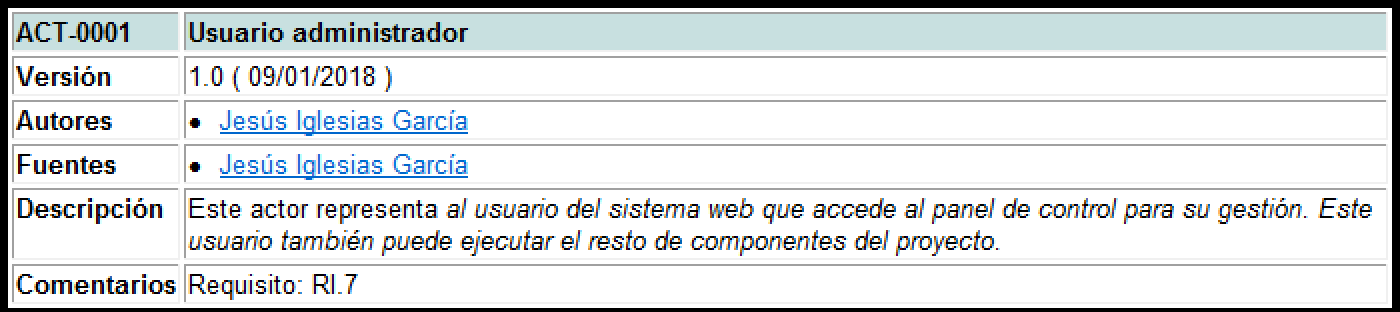
\includegraphics[width=14cm,height=3cm]{Images/analysis/actors/actor_admin} \\
			\label{fig:actor_01} 
		\end{center}  
	\end{figure} 
	
	% NEW PAGE
	\newpage
	
	\begin{figure}[!ht]   
		\caption{Actor - Usuario normal.} 
		\begin{center} 
	 		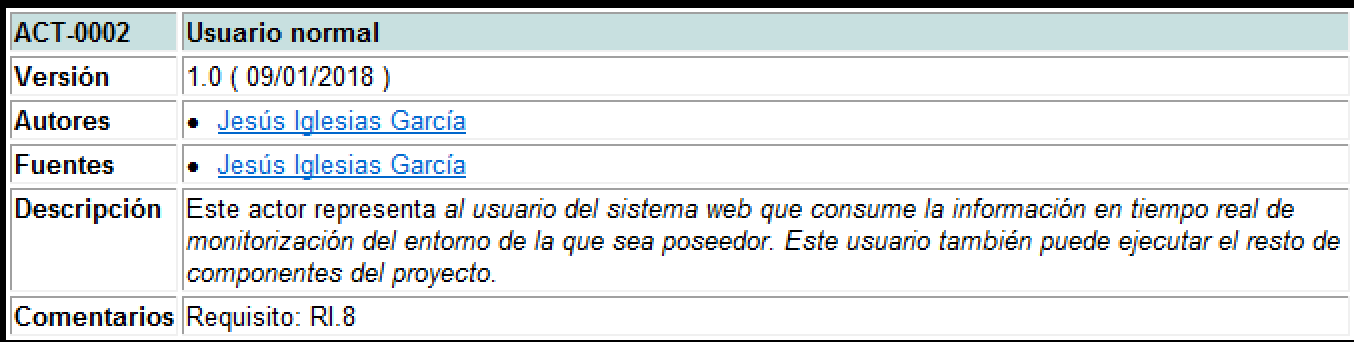
\includegraphics[width=14cm,height=3cm]{Images/analysis/actors/actor_normal} \\
			\label{fig:actor_02} 
		\end{center}  
	\end{figure} 
	
	\begin{figure}[!ht]   
		\caption{Actor - Usuario no registrado.} 
		\begin{center} 
	 		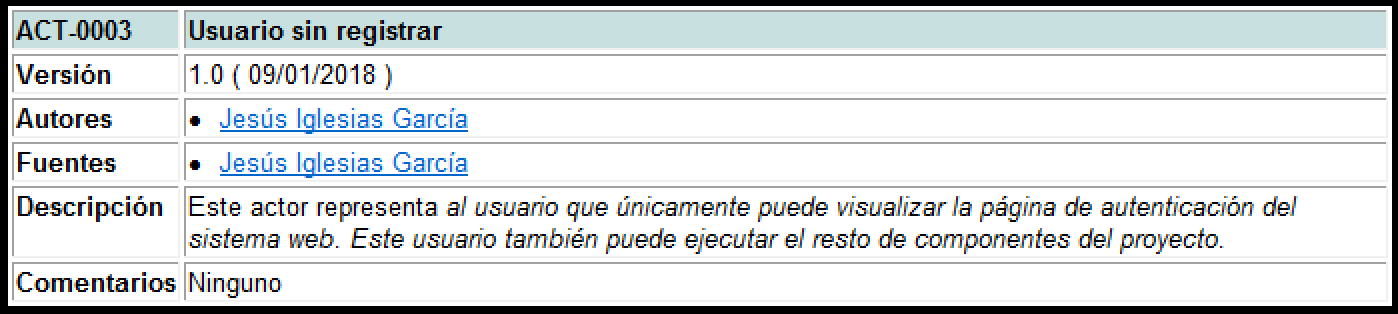
\includegraphics[width=14cm,height=3cm]{Images/analysis/actors/actor_noregistrado} \\
			\label{fig:actor_03} 
		\end{center}  
	\end{figure} 
	
	% Subsection
	\subsection{Lista de casos de uso} \label{UClist}
	
	El siguiente listado muestra los casos de uso identificados:
	
	\begin{itemize}
		\item \textbf{UC-0001:} Configurar dispositivo \gls{raspberry-a}
		\item \textbf{UC-0002:} Monitorizar sucesos del entorno
		\item \textbf{UC-0003:} Desencriptar evidencia
		\item \textbf{UC-0004:} Iniciar sesión
		\item \textbf{UC-0005:} Restablecer contraseña 
		\item \textbf{UC-0006{\color{black!40!blue}*} :} Gestionar usuario administrador
		\item \textbf{UC-0007{\color{black!40!blue}*} :} Gestionar usuario normal
		\item \textbf{UC-0008:} Consultar estadísticas
		\item \textbf{UC-0009:} Consultar o modificar perfil personal
		\item \textbf{UC-0010:} Consumir información sobre la trazabilidad del entorno
	\end{itemize}
	
	{\color{black!40!blue}*} \textbf{¡Importante! -} Como se ha indicado anteriormente, con fines de reducir aquellas partes repetitivas solamente se va a detallar de forma completa el caso de uso UC-0006: Gestionar usuario administrador. El caso de uso UC-0007: Gestionar usuario normal será similar con la salvedad de su adaptación. La gestión de cada entidad engloba las actividades principales de listado, creación, edición, eliminación e importación. A su vez, la actividad listado engloba una serie de subactividades: búsqueda, ordenación, filtrado, elección de columnas (campos de una entidad) a visualizar, restablecimiento de la visualización de las columnas principales, exportación a PDF y CSV, impresión y copiado.

	% Subsection
	\subsection{Diagrama de casos de uso}
	
	El diagrama de casos de uso (Figura \ref{fig:use_case}) tiene como finalidad documentar el comportamiento de un sistema completo desde el punto de vista del usuario.
	
	\begin{figure}[!ht]   
		\caption{Diagrama de casos de uso.} 
		\begin{center} 
	 		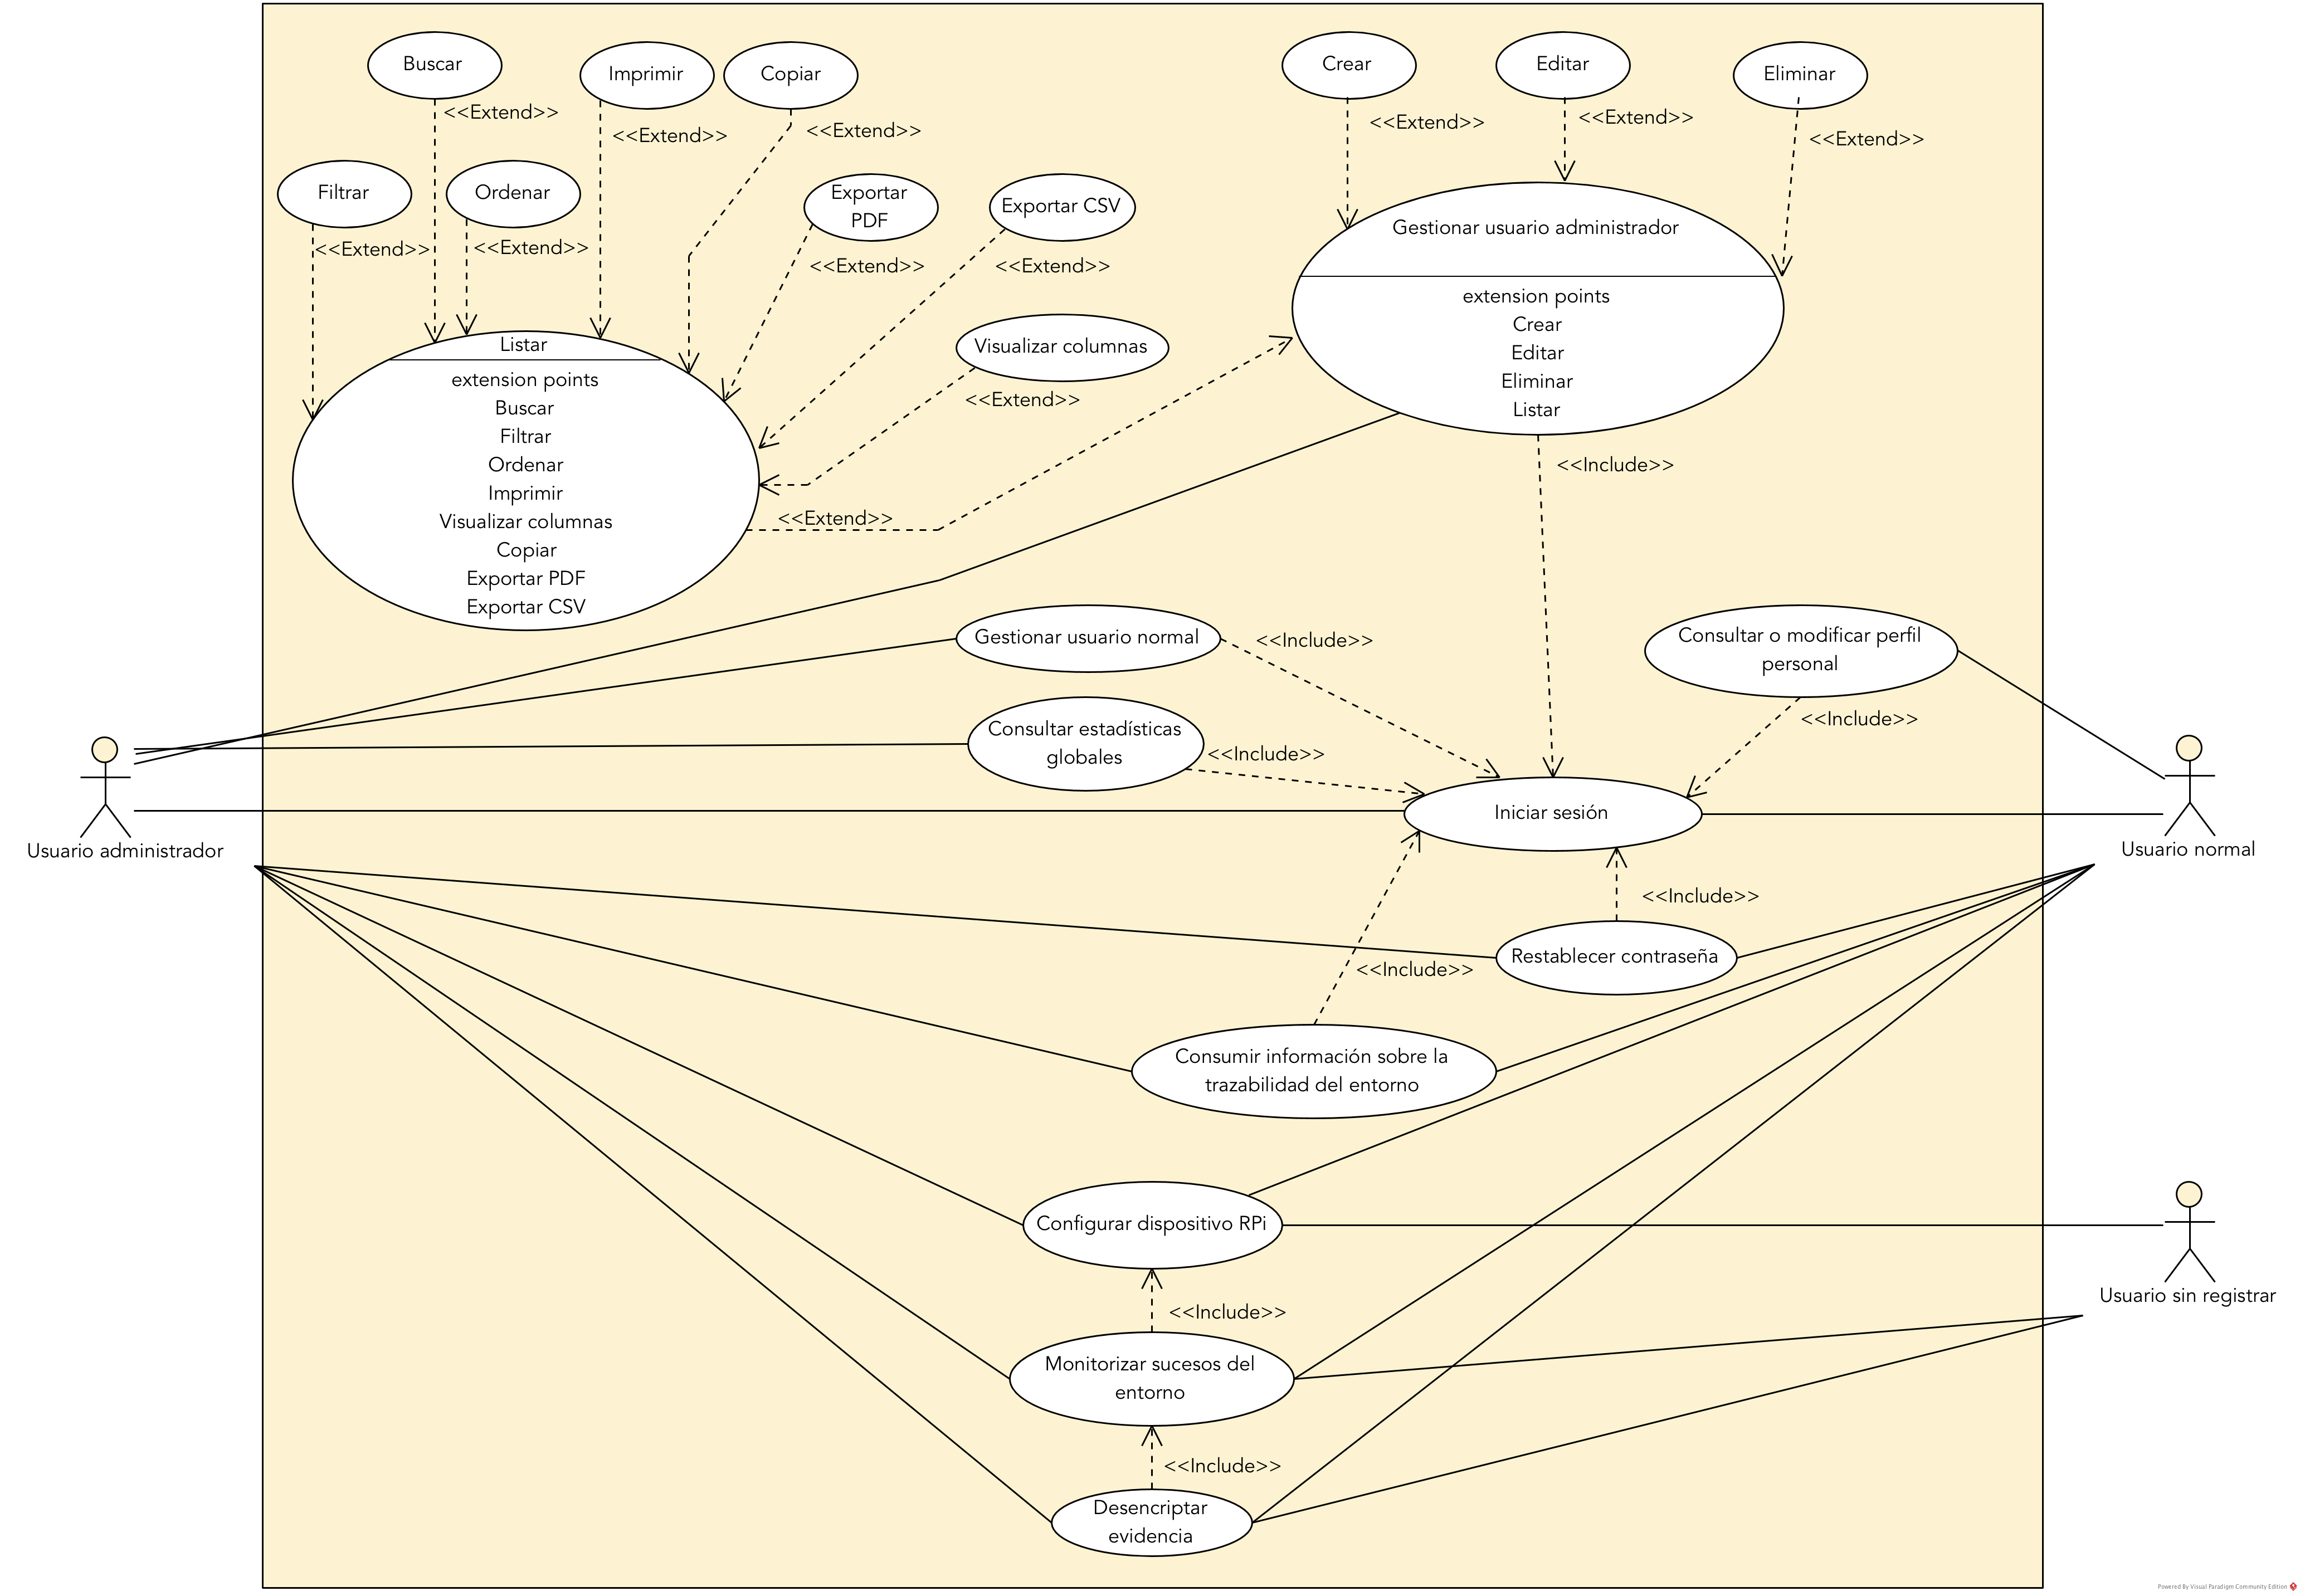
\includegraphics[width=18cm,height=13.5cm]{Images/analysis/useCases} \\
			\label{fig:use_case} 
		\end{center}  
	\end{figure} 	
	
	% Subsection
	\subsection{Descripción de casos de uso}
	
	A continuación se detalla el comportamiento de forma superficial de cada caso de uso identificado, omitiendo en algunos casos todas las acciones realizadas y englobándolas en una acción conjunta con el fin de no alargar demasiado la descripción. \\
	
	% UC-0001 - Configurar dispositivo RPi
	\begin{longtable}{|p{3cm}|p{1cm}|p{12.5cm}|}
		\hline
		\multicolumn{1}{|>{\columncolor{Gainsboro}}c|}{\multirow{1}{*}{\textbf{UC-0001}}} & \multicolumn{2}{|p{13.5cm}|}{\textbf{Configurar dispositivo \gls{raspberry-a}}}
		\\ \hline
		\multicolumn{1}{|>{\columncolor{Gainsboro}}p{3cm}|}{\textbf{Versión}} & \multicolumn{2}{p{13.5cm}|}{1.0 - 12/01/2018 (rev. 15/02/2018)} \\ \hline
		\multicolumn{1}{|>{\columncolor{Gainsboro}}p{3cm}|}{\textbf{Autores}} & \multicolumn{2}{p{13.5cm}|}{Jesús Iglesias García} \\ \hline
		\multicolumn{1}{|>{\columncolor{Gainsboro}}p{3cm}|}{\textbf{Usuario}} & \multicolumn{2}{p{13.5cm}|}{Actor Usuario administrador (ACT-0001), actor Usuario normal (ACT-0002) o actor Usuario sin registrar (ACT-0003)} \\ \hline
		\multicolumn{1}{|>{\columncolor{Gainsboro}}p{3cm}|}{\textbf{Descripción}} & \multicolumn{2}{p{13.5cm}|}{El sistema deberá comportarse tal como se describe en el siguiente caso de uso cuando \textit{cualquiera de los actores identificados quiera realizar la configuración inicial del dispositivo \gls{raspberry-a}}} \\ \hline
		\multicolumn{1}{|>{\columncolor{Gainsboro}}p{3cm}|}{\textbf{Pre-condición}} & \multicolumn{2}{p{13.5cm}|}{El actor se encuentra frente al \gls{prototipo} \textit{hardware} correctamente conectado y funcional} \\ \hline
			
		% Sequence
		\multirow{0}{3cm}{\cellcolor{Gainsboro}\textbf{Secuencia normal}} & \textbf{Paso} & \textbf{Acción}  \\ \cline{2-3} 
		\cellcolor{Gainsboro} & 1 & El caso de uso comienza cuando cualquier de los actores ejecuta este componente \\ \cline{2-3} 
		\cellcolor{Gainsboro} & 2 & El componente realiza una serie de comprobaciones: fichero de utilidades, usuario superprivilegiado, plataforma \gls{gnulinux}, dispositivo \gls{raspberry-a}, conexión de red y concurrencia \\ \cline{2-3} 
		\cellcolor{Gainsboro} & 3 & El componente comprueba las opciones introducidas al ejecutarlo \\ \cline{2-3} 
		\cellcolor{Gainsboro} & 4 & El componente ejecuta la instalación de cada paquete si no se encuentra ya instalado y si existe en el repositorio \\ \cline{2-3} 
		\cellcolor{Gainsboro} & 5 & El componente ejecuta la instalación de cada librería \gls{python} si no se encuentra ya instalada y si existe en el repositorio \\ \cline{2-3} 
		\cellcolor{Gainsboro} & 6 & El componente comprueba que el comando para habilitar interfaces está instalado. En caso afirmativo, comprueba si cada interfaz se encuentra deshabilitada en cuyo caso efectúa la activación de cada una \\ \cline{2-3} 
		\cellcolor{Gainsboro} & 7 & El componente pregunta al usuario si desea reiniciar el dispositivo \\ \cline{2-3} 
		\cellcolor{Gainsboro} & 8 & El actor confirma la acción de reiniciar \\ \cline{2-3} 
		\cellcolor{Gainsboro} & 9 & El componente comprueba que el comando para reiniciar se encuentra instalado y en caso afirmativo reinicia el dispositivo tras 5 segundos de espera \\ \hline

		% Alternative flow
		\multirow{0}{3.2cm}{\cellcolor{Gainsboro}\textbf{Flujo alternativo}} & \textbf{Paso} & \textbf{Acción}  	\\ \cline{2-3} 
		
		\cellcolor{Gainsboro} & 3.1 & El componente comprueba las opciones introducidas detectando que el usuario desea mostrar la ayuda. En dicho caso, muestra la sección informativa, y a continuación el caso de uso finaliza \\ \cline{2-3} 
		\cellcolor{Gainsboro} & 3.2 & El componente comprueba las opciones introducidas detectando que el usuario desea mostrar más información sobre las acciones ejecutadas. En dicho caso, activa el modo \textit{verbose}, y a continuación el caso de uso continúa en el paso 4 \\ \cline{2-3} 
		\cellcolor{Gainsboro} & 3.3 & El componente comprueba las opciones introducidas detectando que el usuario desea ejecutar solamente la instalación de dependencias. En dicho caso, el caso de uso ejecuta solo los pasos 4, 5 y 6 \\ \cline{2-3} 
		\cellcolor{Gainsboro} & 3.4 & El componente comprueba las opciones introducidas detectando que el usuario desea ejecutar solamente la activación de interfaces. En dicho caso, el caso de uso continúa en el paso 7 \\ \cline{2-3} 
						
		\cellcolor{Gainsboro} & 4.1 & El componente verifica si el paquete instalado se encuentra desactualizado. En caso afirmativo, es actualizado \\ \cline{2-3} 
		\cellcolor{Gainsboro} & 4.2 & El componente verifica que cada paquete se encuentra ya instalado y actualizado por lo que no se realiza ninguna acción y el caso de uso continúa en el paso 5 \\ \cline{2-3} 
		\cellcolor{Gainsboro} & 5.1 & El componente verifica si la librería instalada se encuentra desactualizada. En caso afirmativo, es actualizada \\ \cline{2-3} 
		\cellcolor{Gainsboro} & 5.2 & El componente verifica que cada librería se encuentra ya instalada y actualizada por lo que no se realiza ninguna acción y el caso de uso continúa en el paso 6 \\ \cline{2-3} 
		\cellcolor{Gainsboro} & 6.1 & Si el componente comprueba que ambas interfaces ya se encuentran habilitadas, no se realiza la activación y el caso de uso continúa en el paso 8 \\ \cline{2-3}
		\cellcolor{Gainsboro} & 8.1 & El actor indica que no desea reiniciar el dispositivo, y a continuación el caso de uso finaliza \\ \hline

		% Post-condition 
		\multicolumn{1}{|>{\columncolor{Gainsboro}}p{3cm}|}{\textbf{Post-condición}} & \multicolumn{2}{p{13.5cm}|}{El actor ha configurado correctamente el dispositivo y puede entonces ejecutar el componente de monitorización de sucesos del entorno} \\ \hline
			
		% Exceptions
		\multirow{0}{3cm}{\cellcolor{Gainsboro}\textbf{Excepciones}} & \textbf{Paso} & \textbf{Acción}  \\ \cline{2-3}
		\cellcolor{Gainsboro} & 2 & Si alguna de las condiciones iniciales no se cumple, el componente notifica al usuario por el terminal y a continuación, el caso de uso finaliza \\ \cline{2-3}
		\cellcolor{Gainsboro} & 3 & Si el número de opciones introducido es erróneo o alguna opción no es reconocida, el componente notifica al usuario por el terminal, y a continuación el caso de uso finaliza \\ \cline{2-3}
		\cellcolor{Gainsboro} & 4 & Si el paquete no instalado no existe en el repositorio o se produce un error durante la instalación, se notifica al usuario por el terminal y el caso de uso continúa en el paso 4 con el siguiente paquete \\ \cline{2-3}
		\cellcolor{Gainsboro} & 4.1 & Si el componente obtiene algún error durante la actualización de un paquete, se notifica al usuario por el terminal y el caso de uso continúa en el paso 4 con el siguiente paquete \\ \cline{2-3}
		\cellcolor{Gainsboro} & 5 & Si la librería no instalada no existe en el repositorio o se produce un error durante la instalación, se notifica al usuario por el terminal y el caso de uso continúa en el paso 5 con la siguiente librería \\ \cline{2-3}
		\cellcolor{Gainsboro} & 5.1 & Si el componente obtiene algún error durante la actualización de una librería, se notifica al usuario por el terminal y el caso de uso continúa en el paso 5 con la siguiente librería \\ \cline{2-3}
		\cellcolor{Gainsboro} & 6 & Si el componente detecta que el comando para habilitar interfaces no se encuentra instalado o se produce un error durante la activación de alguna interfaz, se muestra una notificación de error y el caso de uso finaliza \\ \cline{2-3}
		\cellcolor{Gainsboro} & 9 & Si el componente detecta que el comando para reiniciar el dispositivo no se encuentra instalado, se muestra una notificación de error y el caso de uso finaliza \\ \hline
				
		\multicolumn{1}{|>{\columncolor{Gainsboro}}p{3cm}|}{\textbf{Comentarios}} & \multicolumn{2}{p{13.5cm}|}{Requisitos: RF.1, RF.2, RF.3, RF.4, RF.5, RF.68, RF.69, RF.70, RF.76} \\ \hline
		\caption{Descripción del caso de uso - Configurar dispositivo RPi}
	\end{longtable}
	
	% UC-0002 - Monitorizar sucesos del entorno
	\begin{longtable}{|p{3cm}|p{1cm}|p{12.5cm}|}
		\hline
		\multicolumn{1}{|>{\columncolor{Gainsboro}}c|}{\multirow{1}{*}{\textbf{UC-0002}}} & \multicolumn{2}{|p{13.5cm}|}{\textbf{Monitorizar sucesos del entorno}}
		\\ \hline
		\multicolumn{1}{|>{\columncolor{Gainsboro}}p{3cm}|}{\textbf{Versión}} & \multicolumn{2}{p{13.5cm}|}{1.0 - 12/01/2018 (rev. 15/02/2018)} \\ \hline
		\multicolumn{1}{|>{\columncolor{Gainsboro}}p{3cm}|}{\textbf{Autores}} & \multicolumn{2}{p{13.5cm}|}{Jesús Iglesias García} \\ \hline
		\multicolumn{1}{|>{\columncolor{Gainsboro}}p{3cm}|}{\textbf{Usuario}} & \multicolumn{2}{p{13.5cm}|}{Actor Usuario administrador (ACT-0001), actor Usuario normal (ACT-0002) o actor Usuario sin registrar (ACT-0003)} \\ \hline
		\multicolumn{1}{|>{\columncolor{Gainsboro}}p{3cm}|}{\textbf{Descripción}} & \multicolumn{2}{p{13.5cm}|}{El sistema deberá comportarse tal como se describe en el siguiente caso de uso cuando \textit{cualquiera de los actores identificados quiera monitorizar los sucesos que se producen en el entorno}} \\ \hline
		\multicolumn{1}{|>{\columncolor{Gainsboro}}p{3cm}|}{\textbf{Pre-condición}} & \multicolumn{2}{p{13.5cm}|}{El actor posee el \gls{prototipo} \textit{hardware} correctamente conectado y configurado} \\ \hline
			
		% Sequence
		\multirow{0}{3cm}{\cellcolor{Gainsboro}\textbf{Secuencia normal}} & \textbf{Paso} & \textbf{Acción}  \\ \cline{2-3} 
		\cellcolor{Gainsboro} & 1 & El caso de uso comienza cuando cualquiera de los actores ejecuta este componente \\ \cline{2-3}  
		\cellcolor{Gainsboro} & 2 & El componente realiza una serie de comprobaciones iniciales: usuario superprivilegiado, plataforma \gls{gnulinux}, dispositivo \gls{raspberry-a}, conexión de red y concurrencia \\ \cline{2-3}  
		\cellcolor{Gainsboro} & 3 & El componente inicializa el \textit{logger} \\ \cline{2-3}  
		\cellcolor{Gainsboro} & 4 & El componente comprueba las opciones introducidas al ejecutarlo \\ \cline{2-3}  
		\cellcolor{Gainsboro} & 5 & El componente solicita las credenciales y datos de configuración de las distintas utilidades y servicios \\ \cline{2-3}  
		\cellcolor{Gainsboro} & 6 & El usuario introduce la información \\ \cline{2-3}  
		\cellcolor{Gainsboro} & 7 & El componente inicializa cada utilidad y servicio \\ \cline{2-3}  
		\cellcolor{Gainsboro} & 8 & El componente monitoriza los sucesos del entorno mediante la obtención de una medición, mostrando la información por el terminal y los \glspl{lcd-a} \\ \cline{2-3}  
		\cellcolor{Gainsboro} & 9 & El componente comprueba si la medición actual representa un suceso anómalo. En caso afirmativo, activa el protocolo de alerta \\ \cline{2-3}  
		\cellcolor{Gainsboro} & 10 & El componente efectúa las acciones del protocolo de alerta: capturar evidencia (vídeo), calcular código \textit{hash}, encriptar y firmar la evidencia, almacenar la evidencia en la nube, almacenar medición en la \gls{bbdd-a}, enviar el suceso a la plataforma \gls{iot-a}, registrar la alerta en la \gls{blockchain-a} y notificar por \textit{email} en caso de que dicha opción esté activa \\ \cline{2-3}  	
		\cellcolor{Gainsboro} & 11 & El caso de uso vuelve al paso 8 \\ \hline
		
		% Alternative flow
		\multirow{0}{3.2cm}{\cellcolor{Gainsboro}\textbf{Flujo alternativo}} & \textbf{Paso} & \textbf{Acción}  	\\ \cline{2-3}
		\cellcolor{Gainsboro} & 4.1 & El componente comprueba las opciones introducidas detectando que el usuario desea mostrar la ayuda. En dicho caso, muestra la sección informativa, y a continuación el caso de uso finaliza \\ \cline{2-3}
 		\cellcolor{Gainsboro} & 9.1 & El componente comprueba si la medición actual representa un suceso anómalo. En caso negativo, no activa ningún protocolo \\ \cline{2-3} 
		\cellcolor{Gainsboro} & 9.1.1 & El componente efectúa las acciones de una medición normal: almacenar medición en la \gls{bbdd-a}, enviar el suceso a la plataforma \gls{iot-a} \\ \cline{2-3}
		\cellcolor{Gainsboro} & 9.1.2 & El caso de uso vuelve al paso 8 \\ \cline{2-3}
		\cellcolor{Gainsboro} & 9.2 & El componente comprueba si la medición actual es errónea. En caso afirmativo, no muestra ningún valor por el terminal ni los \glspl{lcd-a} y a continuación, el caso de uso vuelve al paso 8 \\ \hline

		% Post-condition 
		\multicolumn{1}{|>{\columncolor{Gainsboro}}p{3cm}|}{\textbf{Post-condición}} & \multicolumn{2}{p{13.5cm}|}{El actor ha monitorizado el entorno \gls{iot-a} registrando tanto los sucesos normales como aquellos considerados anómalos} \\ \hline
			
		% Exceptions
		\multirow{0}{3cm}{\cellcolor{Gainsboro}\textbf{Excepciones}} & \textbf{Paso} & \textbf{Acción}  \\ \cline{2-3}
		\cellcolor{Gainsboro} & 2 & Si alguna de las condiciones iniciales no se cumple, el componente notifica al usuario por el terminal y a continuación, el caso de uso finaliza \\ \cline{2-3}
		\cellcolor{Gainsboro} & 3 & Si el componente obtiene algún error durante la creación del directorio donde se almacenará el fichero de \textit{log}, se notifica al usuario por el terminal y a continuación, el caso de uso finaliza \\ \cline{2-3}
		\cellcolor{Gainsboro} & 4 & Si el número de opciones introducido es erróneo, alguna opción presenta un valor incorrecto o no es reconocida, el componente notifica al usuario por el terminal y a continuación, el caso de uso finaliza \\ \cline{2-3}
		\cellcolor{Gainsboro} & 	7 & Si el componente obtiene algún error durante la inicialización de alguna utilidad o servicio, se notifica al usuario por el terminal y a continuación, el caso de uso finaliza \\ \cline{2-3}
		\cellcolor{Gainsboro} & 9.1.1 & Si el componente obtiene algún error durante la ejecución de alguna acción tras una medición normal, se notifica al usuario por el terminal, se envía un \textit{email} del error en caso de estar activa dicha opción y a continuación, el caso de uso finaliza \\ \cline{2-3}
		\cellcolor{Gainsboro} & 10 & Si el componente obtiene algún error durante la ejecución de alguna acción del protocolo de alerta, se notifica al usuario por el terminal, se envía un \textit{email} del error en caso de estar activa dicha opción y a continuación, el caso de uso finaliza \\ \hline
				
		\multicolumn{1}{|>{\columncolor{Gainsboro}}p{3cm}|}{\textbf{Comentarios}} & \multicolumn{2}{p{13.5cm}|}{Requisitos: RF.6, RF.7, RF.8, RF.9, RF.10, RF.11, RF.12, RF.13, RF.14, RF.15, RF.16, RF.17, RF.18, RF.19, RF.20, RF.21, RF.22, RF.23, RF.24, RF.25, RF.26, RF.27, RF.28, RF.29, RF.30, RF.31, RF.32, RF.33, RF.34, RF.35, RF.36, RF.37, RF.38, RF.39, RF.40, RF.41, RF.42, RF.43, RF.44, RF.45, RF.46, RF.47, RF.48, RF.49, RF.50, RF.51, RF.52, RF.53, RF.54, RF.60, RF.61, RF.67, RF.68, RF.69, RF.71, RF.72, RF.73, RF.74, RF.75, RF.76} \\ \hline
		\caption{Descripción del caso de uso - Monitorizar sucesos del entorno}
	\end{longtable}
		
	% UC-0003 - Desencriptar evidencia
	\begin{longtable}{|p{3cm}|p{1cm}|p{12.5cm}|}
		\hline
		\multicolumn{1}{|>{\columncolor{Gainsboro}}c|}{\multirow{1}{*}{\textbf{UC-0003}}} & \multicolumn{2}{|p{13.5cm}|}{\textbf{Desencriptar evidencia}}
		\\ \hline
		\multicolumn{1}{|>{\columncolor{Gainsboro}}p{3cm}|}{\textbf{Versión}} & \multicolumn{2}{p{13.5cm}|}{1.0 - 12/01/2018 (rev. 15/02/2018)} \\ \hline
		\multicolumn{1}{|>{\columncolor{Gainsboro}}p{3cm}|}{\textbf{Autores}} & \multicolumn{2}{p{13.5cm}|}{Jesús Iglesias García} \\ \hline
		\multicolumn{1}{|>{\columncolor{Gainsboro}}p{3cm}|}{\textbf{Usuario}} & \multicolumn{2}{p{13.5cm}|}{Actor Usuario administrador (ACT-0001), actor Usuario normal (ACT-0002) o actor Usuario sin registrar (ACT-0003)} \\ \hline
		\multicolumn{1}{|>{\columncolor{Gainsboro}}p{3cm}|}{\textbf{Descripción}} & \multicolumn{2}{p{13.5cm}|}{El sistema deberá comportarse tal como se describe en el siguiente caso de uso cuando \textit{cualquiera de los actores identificados quiera desencriptar una evidencia previamente encriptada con \gls{gpg-a}, verificar la firma y la integridad de su contenido}} \\ \hline
		\multicolumn{1}{|>{\columncolor{Gainsboro}}p{3cm}|}{\textbf{Pre-condición}} & \multicolumn{2}{p{13.5cm}|}{El actor posee la evidencia, acceso al par de claves usado durante la encriptación y firmado y el código \textit{hash} del contenido de la evidencia} \\ \hline
			
		% Sequence
		\multirow{0}{3cm}{\cellcolor{Gainsboro}\textbf{Secuencia normal}} & \textbf{Paso} & \textbf{Acción}  \\ \cline{2-3} 
		\cellcolor{Gainsboro} & 1 & El caso de uso comienza cuando cualquiera de los actores ejecuta este componente \\ \cline{2-3} 
		\cellcolor{Gainsboro} & 2 & El componente comprueba que la ejecución se efectuó con un usuario superprivilegiado \\ \cline{2-3} 
		\cellcolor{Gainsboro} & 3 & El componente comprueba las opciones introducidas al ejecutarlo \\ \cline{2-3} 
		\cellcolor{Gainsboro} & 4 & El componente descarga de la nube la evidencia encriptada y firmada en caso de introducir la opción correspondiente \\ \cline{2-3} 
		\cellcolor{Gainsboro} & 5 & El componente comprueba la existencia en el sistema local de los ficheros (evidencia, par de claves) y directorios indicados en las opciones \\ \cline{2-3} 
		\cellcolor{Gainsboro} & 6 & El componente comprueba que la evidencia posea el formato correcto \\ \cline{2-3} 
		\cellcolor{Gainsboro} & 7 & El componente importa el par de claves desde el fichero indicado \\ \cline{2-3} 
		\cellcolor{Gainsboro} & 8 & El componente solicita la contraseña de protección de la clave privada \\ \cline{2-3} 
		\cellcolor{Gainsboro} & 9 & El actor introduce la credencial \\ \cline{2-3} 
		\cellcolor{Gainsboro} & 10 & El componente comprueba que el dato introducido no sea vacío \\ \cline{2-3} 
		\cellcolor{Gainsboro} & 11 & El componente desencripta la evidencia \\ \cline{2-3} 
		\cellcolor{Gainsboro} & 12 & El componente verifica la firma \\ \cline{2-3} 
		\cellcolor{Gainsboro} & 13 & El componente calcula el código \textit{hash} de la evidencia recién desencriptada y lo compara con el valor \textit{hash} introducido \\ \hline

		% Alternative flow
		\multirow{0}{3.2cm}{\cellcolor{Gainsboro}\textbf{Flujo alternativo}} & \textbf{Paso} & \textbf{Acción} \\ \cline{2-3} 
		
		\cellcolor{Gainsboro} & 3.1 & El componente comprueba las opciones introducidas detectando que el usuario desea mostrar la ayuda. En dicho caso, muestra la sección informativa, y a continuación el caso de uso finaliza \\ \cline{2-3} 
		\cellcolor{Gainsboro} & 7.1 & El componente comprueba que la huella digital o \textit{fingerprint} introducida se relacione con el de alguna clave existente en el almacén de claves \\ \cline{2-3} 
		\cellcolor{Gainsboro} & 12.1 & El componente verifica que la evidencia no fue firmada \\ \hline

		% Post-condition 
		\multicolumn{1}{|>{\columncolor{Gainsboro}}p{3cm}|}{\textbf{Post-condición}} & \multicolumn{2}{p{13.5cm}|}{El actor ha desencriptado la evidencia y ha comprobado la firma y la integridad del contenido} \\ \hline
			
		% Exceptions
		\multirow{0}{3cm}{\cellcolor{Gainsboro}\textbf{Excepciones}} & \textbf{Paso} & \textbf{Acción}  \\ \cline{2-3}
		\cellcolor{Gainsboro} & 2 & El componente detecta que la ejecución fue con un usuario normal, por lo que notifica al usuario del error, y a continuación el caso de uso finaliza \\ \cline{2-3}
		\cellcolor{Gainsboro} & 3 & Si el número de opciones introducido es erróneo, no se ha introducido alguna opción obligatoria, alguna opción presenta un valor incorrecto o no es reconocida, el componente notifica al usuario por el terminal y a continuación, el caso de uso finaliza \\ \cline{2-3}
		\cellcolor{Gainsboro} & 5 & Si el componente verifica que algún fichero o directorio no existe o no es del tipo correcto, notifica al usuario por el terminal, y a continuación el caso de uso finaliza \\ \cline{2-3}
		\cellcolor{Gainsboro} & 6 & Si el componente verifica que la evidencia posee un formato distinto al permitido, notifica al usuario por el terminal, y a continuación el caso de uso finaliza \\ \cline{2-3}
		\cellcolor{Gainsboro} & 7 & Si el componente verifica que el fichero no contiene el par de claves, notifica al usuario por el terminal, y a continuación el caso de uso finaliza \\ \cline{2-3}
		\cellcolor{Gainsboro} & 7.1 & Si el componente verifica que el almacén de claves no contiene ninguna clave o el \textit{fingerprint} no se relaciona con el de alguna clave existente en el almacén, notifica al usuario por el terminal, y a continuación el caso de uso finaliza \\ \cline{2-3}
		\cellcolor{Gainsboro} & 10 & Si el componente verifica que la credencial introducida son espacios en blanco, notifica al usuario por el terminal siempre y cuando haya gastado el número de intentos (3), y a continuación el caso de uso finaliza \\ \cline{2-3}
		\cellcolor{Gainsboro} & 11 & Si el componente obtiene algún error durante la desencriptación, notifica al usuario por el terminal, y a continuación el caso de uso finaliza \\ \cline{2-3}
		\cellcolor{Gainsboro} & 13 & Si el componente obtiene algún error durante el cálculo del valor \textit{hash}, notifica al usuario por el terminal, y a continuación el caso de uso finaliza \\ \hline
				
		\multicolumn{1}{|>{\columncolor{Gainsboro}}p{3cm}|}{\textbf{Comentarios}} & \multicolumn{2}{p{13.5cm}|}{Requisitos: RF.55, RF.56, RF.57, RF.58, RF.59, RF.60, RF.61, RF.62, RF.63, RF.64, RF.65, RF.66, RF.67, RF.68, RF.69, RF.73, RF.74, RF.76} \\ \hline
		\caption{Descripción del caso de uso - Desencriptar evidencia}
	\end{longtable}
	
	% VSPACE
	\vspace{0.5cm}
	
	% UC-0004 - Iniciar sesión
	\begin{longtable}{|p{3cm}|p{1cm}|p{12.5cm}|}
		\hline
		\multicolumn{1}{|>{\columncolor{Gainsboro}}c|}{\multirow{1}{*}{\textbf{UC-0004}}} & \multicolumn{2}{|p{13.5cm}|}{\textbf{Iniciar sesión}}
		\\ \hline
		\multicolumn{1}{|>{\columncolor{Gainsboro}}p{3cm}|}{\textbf{Versión}} & \multicolumn{2}{p{13.5cm}|}{1.0 - 12/01/2018 (rev. 16/02/2018)} \\ \hline
		\multicolumn{1}{|>{\columncolor{Gainsboro}}p{3cm}|}{\textbf{Autores}} & \multicolumn{2}{p{13.5cm}|}{Jesús Iglesias García} \\ \hline
		\multicolumn{1}{|>{\columncolor{Gainsboro}}p{3cm}|}{\textbf{Usuario}} & \multicolumn{2}{p{13.5cm}|}{Actor Usuario administrador (ACT-0001) o actor Usuario normal (ACT-0002)} \\ \hline
		\multicolumn{1}{|>{\columncolor{Gainsboro}}p{3cm}|}{\textbf{Descripción}} & \multicolumn{2}{p{13.5cm}|}{El sistema deberá comportarse tal como se describe en el siguiente caso de uso cuando \textit{un actor Usuario administrador (ACT-0001) o  actor Usuario normal (ACT-0002) quiera iniciar sesión en el sistema web}} \\ \hline
		\multicolumn{1}{|>{\columncolor{Gainsboro}}p{3cm}|}{\textbf{Pre-condición}} & \multicolumn{2}{p{13.5cm}|}{El actor Usuario administrador (ACT-0001) o  actor Usuario normal (ACT-0002) se encuentra en la página de inicio del sistema web} \\ \hline
			
		% Sequence
		\multirow{0}{3cm}{\cellcolor{Gainsboro}\textbf{Secuencia normal}} & \textbf{Paso} & \textbf{Acción}  \\ \cline{2-3} 
		\cellcolor{Gainsboro} & 1 & El caso de uso comienza cuando un actor Usuario administrador (ACT-0001) o actor Usuario normal (ACT-0002) introduce sus credenciales para la autenticación  		\\ \cline{2-3} 
		\cellcolor{Gainsboro} & 2 & El sistema web comprueba que los datos introducidos sean correctos. En caso afirmativo, crea la sesión de usuario y le redirige a la página de usuario dentro del sistema, si éste posee rol usuario normal 		\\ \hline

		% Alternative flow
		\multirow{0}{3.2cm}{\cellcolor{Gainsboro}\textbf{Flujo alternativo}} & \textbf{Paso} & \textbf{Acción}  	\\ \cline{2-3} 
		\cellcolor{Gainsboro} & 1.1 & El sistema web comprueba si existe la \textit{\gls{cookie}} referente a la funcionalidad de \textit{Recordarme}. En caso afirmativo, el sistema web inicia sesión automáticamente al usuario y le redirige a la página de usuario dentro del sistema o al panel de control según su rol. A continuación, el caso de uso finaliza \\ \cline{2-3} 
		\cellcolor{Gainsboro} & 2.1 & El sistema web comprueba que los datos introducidos sean correctos. En caso afirmativo, crea la sesión de usuario y le redirige al panel de control, si éste posee rol usuario administrador \\ \hline

		% Post-condition 
		\multicolumn{1}{|>{\columncolor{Gainsboro}}p{3cm}|}{\textbf{Post-condición}} & \multicolumn{2}{p{13.5cm}|}{El actor Usuario administrador (ACT-0001) o  actor Usuario normal (ACT-0002) ha iniciado sesión en el sistema web y se encuentra dentro de él ya sea en el panel de control o en la página de usuario según el rol de éste} \\ \hline
			
		% Exceptions
		\multirow{0}{3cm}{\cellcolor{Gainsboro}\textbf{Excepciones}} & \textbf{Paso} & \textbf{Acción}  \\ \cline{2-3}
		\cellcolor{Gainsboro} & 1.1 & Si la \textit{\gls{cookie}} referente a la funcionalidad de \textit{Recordarme} no existe, el sistema web redirige a la página de inicio, y a continuación el caso de uso finaliza \\ \cline{2-3}
		\cellcolor{Gainsboro} & 2, 2.1 & Si el sistema web obtiene algún error al comprobar los datos introducidos (datos erróneos, usuario no registrado, cuenta bloqueada, cuenta sin activar, cuenta o contraseña expirada), muestra un mensaje de error, y a continuación el caso de uso finaliza. En el caso de que sea el 5 intento fallido, también se realiza la acción de bloquear la cuenta de usuario \\ \hline
				
		\multicolumn{1}{|>{\columncolor{Gainsboro}}p{3cm}|}{\textbf{Comentarios}} & \multicolumn{2}{p{13.5cm}|}{Requisitos: RF.77, RF.78, RF.79, RF.80} \\ \hline
		\caption{Descripción del caso de uso - Iniciar sesión}
	\end{longtable}
	
	% VSPACE
	\vspace{1cm}
	
	% UC-0005 - Restablecer contraseña
	\begin{longtable}{|p{3cm}|p{1cm}|p{12.5cm}|}
		\hline
		\multicolumn{1}{|>{\columncolor{Gainsboro}}c|}{\multirow{1}{*}{\textbf{UC-0005}}} & \multicolumn{2}{|p{13.5cm}|}{\textbf{Restablecer contraseña}}
		\\ \hline
		\multicolumn{1}{|>{\columncolor{Gainsboro}}p{3cm}|}{\textbf{Versión}} & \multicolumn{2}{p{13.5cm}|}{1.0 - 13/01/2018 (rev. 16/02/2018)} \\ \hline
		\multicolumn{1}{|>{\columncolor{Gainsboro}}p{3cm}|}{\textbf{Autores}} & \multicolumn{2}{p{13.5cm}|}{Jesús Iglesias García} \\ \hline
		\multicolumn{1}{|>{\columncolor{Gainsboro}}p{3cm}|}{\textbf{Usuario}} & \multicolumn{2}{p{13.5cm}|}{Actor Usuario administrador (ACT-0001) o actor Usuario normal (ACT-0002)} \\ \hline
		\multicolumn{1}{|>{\columncolor{Gainsboro}}p{3cm}|}{\textbf{Descripción}} & \multicolumn{2}{p{13.5cm}|}{El sistema web deberá comportarse tal como se describe en el siguiente caso de uso cuando \textit{un actor Usuario administrador (ACT-0001) o  actor Usuario normal (ACT-0002) quiera restablecer su contraseña}} \\ \hline
		\multicolumn{1}{|>{\columncolor{Gainsboro}}p{3cm}|}{\textbf{Pre-condición}} & \multicolumn{2}{p{13.5cm}|}{El actor Usuario administrador (ACT-0001) o actor Usuario normal (ACT-0002) se encuentra en la página de inicio del sistema web} \\ \hline
			
		% Sequence
		\multirow{0}{3cm}{\cellcolor{Gainsboro}\textbf{Secuencia normal}} & \textbf{Paso} & \textbf{Acción}  \\ \cline{2-3} 
		\cellcolor{Gainsboro} & 1 & El caso de uso comienza cuando un actor Usuario administrador (ACT-0001) o actor Usuario normal (ACT-0002) selecciona la opción para restablecer la contraseña 		\\ \cline{2-3} 
		\cellcolor{Gainsboro} & 2 & El sistema web muestra el formulario a rellenar \\ \cline{2-3}  
		\cellcolor{Gainsboro} & 3 & El actor Usuario administrador (ACT-0001) o actor Usuario normal (ACT-0002) introduce su \textit{email} asociado a su cuenta existente \\ \cline{2-3} 
		\cellcolor{Gainsboro} & 4 & El sistema web comprueba que el \textit{email} introducido es correcto. En caso afirmativo, envía al usuario un correo electrónico de restablecimiento de la contraseña y le avisa mediante un mensaje				\\ \cline{2-3} 
		\cellcolor{Gainsboro} & 5 & El actor Usuario administrador (ACT-0001) o actor Usuario normal (ACT-0002) restablece su contraseña a través del correo de restablecimiento 	\\ \cline{2-3} 
		\cellcolor{Gainsboro} & 6 & El sistema comprueba que la nueva contraseña sea correcta. En caso afirmativo, asigna la nueva contraseña al usuario y muestra la página de inicio del sistema 	\\ \hline

		% Post-condition 
		\multicolumn{1}{|>{\columncolor{Gainsboro}}p{3cm}|}{\textbf{Post-condición}} & \multicolumn{2}{p{13.5cm}|}{El actor Usuario administrador (ACT-0001) o  actor Usuario normal (ACT-0002) ha modificado su contraseña} \\ \hline
					
		% Exceptions
		\multirow{0}{3cm}{\cellcolor{Gainsboro}\textbf{Excepciones}} & \textbf{Paso} & \textbf{Acción} \\ \cline{2-3} 
		\cellcolor{Gainsboro} & 3 & Si el actor Usuario administrador (ACT-0001) o actor Usuario normal (ACT-0002) cancela la introducción del \textit{email} en el formulario, el sistema web no realiza ninguna acción, y a continuación el caso de uso finaliza		\\ \cline{2-3} 
		\cellcolor{Gainsboro} & 4 & Si el sistema web obtiene algún error al comprobar el \textit{email} introducido (dirección de correo inexistente), muestra un mensaje, y a continuación el caso de uso vuelve al paso 2	\\ \cline{2-3} 
		\cellcolor{Gainsboro} & 4 & Si el sistema web obtiene algún error al enviar el \textit{email}, muestra un mensaje de error y el caso de uso finaliza			\\ \cline{2-3} 
		\cellcolor{Gainsboro} & 6 & Si el sistema web obtiene algún error al comprobar el \textit{\gls{token}} de seguridad (expirado, ya usado o de distinto tipo) de restablecimiento de contraseña, muestra un mensaje de error y el caso de uso finaliza	\\ \cline{2-3}
		\cellcolor{Gainsboro} & 6 & Si el sistema web obtiene algún error al comprobar la nueva contraseña (no cumple con un patrón), muestra un mensaje de error, y a continuación el caso de uso vuelve al paso 5	\\ \hline
				
		\multicolumn{1}{|>{\columncolor{Gainsboro}}p{3cm}|}{\textbf{Comentarios}} & \multicolumn{2}{p{13.5cm}|}{Requisitos: RF.81} \\ \hline
		\caption{Descripción del caso de uso - Restablecer contraseña}
	\end{longtable}
	
	% UC-0006 - Gestionar usuario administrador
	\begin{longtable}{|p{3cm}|p{1cm}|p{12.5cm}|}
		\hline
		\multicolumn{1}{|>{\columncolor{Gainsboro}}c|}{\multirow{1}{*}{\textbf{UC-0006}}{\color{black!40!blue}*}} & \multicolumn{2}{|p{13.5cm}|}{\textbf{Gestionar usuario administrador}}
		\\ \hline
		\multicolumn{1}{|>{\columncolor{Gainsboro}}p{3cm}|}{\textbf{Versión}} & \multicolumn{2}{p{13.5cm}|}{1.0 - 13/01/2018 (rev. 16/02/2018)} \\ \hline
		\multicolumn{1}{|>{\columncolor{Gainsboro}}p{3cm}|}{\textbf{Autores}} & \multicolumn{2}{p{13.5cm}|}{Jesús Iglesias García} \\ \hline
		\multicolumn{1}{|>{\columncolor{Gainsboro}}p{3cm}|}{\textbf{Usuario}} & \multicolumn{2}{p{13.5cm}|}{Actor Usuario administrador (ACT-0001)} \\ \hline
		\multicolumn{1}{|>{\columncolor{Gainsboro}}p{3cm}|}{\textbf{Descripción}} & \multicolumn{2}{p{13.5cm}|}{El sistema web deberá comportarse tal como se describe en el siguiente caso de uso cuando \textit{un actor Usuario administrador (ACT-0001)} quiera gestionar un usuario administrador} \\ \hline
		\multicolumn{1}{|>{\columncolor{Gainsboro}}p{3cm}|}{\textbf{Pre-condición}} & \multicolumn{2}{p{13.5cm}|}{El actor Usuario administrador (ACT-0001) debe estar autenticado en el sistema web} \\ \hline
			
		% Sequence
		\multirow{0}{3cm}{\cellcolor{Gainsboro}\textbf{Secuencia}} & \textbf{Paso} & \textbf{Acción}  \\ \cline{2-3} 
		\cellcolor{Gainsboro} & 1 & El caso de uso comienza cuando el actor Usuario administrador (ACT-0001) notifica desde el panel de control que desea gestionar un usuario administrador 			\\ \cline{2-3} 
		\cellcolor{Gainsboro} & 2 & El sistema web muestra un listado ordenado y paginado o filtrado de los usuarios administradores disponibles en el sistema \\\cline{2-3} 
		\cellcolor{Gainsboro} & 3 & El actor Usuario administrador (ACT-0001) selecciona el apartado para crear un nuevo usuario administrador \\\cline{2-3} 
		\cellcolor{Gainsboro} & 4 & El sistema web muestra el formulario con los campos a rellenar del nuevo usuario \\\cline{2-3} 
		\cellcolor{Gainsboro} & 5 & El actor Usuario administrador (ACT-0001) completa los datos del formulario \\\cline{2-3} 
		\cellcolor{Gainsboro} & 6 & El sistema web comprueba que los datos introducidos sean correctos. En caso afirmativo, almacena el nuevo usuario con rol usuario administrador y avisa al actor Usuario administrador (ACT-0001) mediante un mensaje. A continuación, el caso de uso vuelve al paso 2 \\ \hline

		% Alternative flow
		\multirow{0}{3.2cm}{\cellcolor{Gainsboro}\textbf{Flujo alternativo}} & \textbf{Paso} & \textbf{Acción}  	\\ \cline{2-3} 
		\cellcolor{Gainsboro} & 1.1.1 & El actor Usuario administrador (ACT-0001) notifica desde el panel de administración que desea importar un usuario administrador o varios \\ \cline{2-3} 
		\cellcolor{Gainsboro} & 1.1.2 & El sistema web muestra la página para la importación con las instrucciones informativas \\ \cline{2-3} 
		\cellcolor{Gainsboro} & 1.1.3 & El actor Usuario administrador (ACT-0001) selecciona el fichero a importar \\ \cline{2-3} 
		\cellcolor{Gainsboro} & 1.1.4 & El sistema web comprueba que el fichero y su contenido es válido. En caso afirmativo, almacena el usuario administrador o usuarios administradores y avisa al actor Usuario administrador (ACT-0001) mediante un mensaje. A continuación, el caso de uso vuelve al paso 1.1.2 \\ \cline{2-3}
		\cellcolor{Gainsboro} & 3.1.1 & El actor Usuario administrador (ACT-0001) selecciona un usuario administrador existente para su edición \\ \cline{2-3} 
		\cellcolor{Gainsboro} & 3.1.2 & El sistema web muestra el formulario con los datos del usuario administrador seleccionado \\ \cline{2-3} 
		\cellcolor{Gainsboro} & 3.1.3 & El actor Usuario administrador (ACT-0001) edita los campos deseados \\ \cline{2-3} 
		\cellcolor{Gainsboro} & 3.1.4 & El sistema web comprueba que los datos editados sean correctos. En caso afirmativo, almacena el usuario modificado y avisa al actor Usuario administrador (ACT-0001) mediante un mensaje. A continuación, el caso de uso vuelve al paso 2 \\ \cline{2-3} 
		\cellcolor{Gainsboro} & 3.2.1 & El actor Usuario administrador (ACT-0001) selecciona un usuario administrador existente para eliminarle \\ \cline{2-3} 
		\cellcolor{Gainsboro} & 3.2.2 & El sistema web muestra un \textit{pop-up} de confirmación \\ \cline{2-3} 
		\cellcolor{Gainsboro} & 3.2.3 & El actor Usuario administrador (ACT-0001) confirma la eliminación \\ \cline{2-3} 
		\cellcolor{Gainsboro} & 3.2.4 & El sistema web elimina el usuario administrador seleccionado y avisa al actor Usuario administrador (ACT-0001) mediante un mensaje. A continuación, el caso de uso vuelve al paso 2 \\ \cline{2-3} 
		\cellcolor{Gainsboro} & 3.3.1 & El actor Usuario administrador (ACT-0001) introduce una cadena de caracteres para realizar una búsqueda entre todos los usuarios administradores existentes. A continuación, el caso de uso vuelve al paso 2 \\ \cline{2-3} 
		\cellcolor{Gainsboro} & 3.4.1 & El actor Usuario administrador (ACT-0001) selecciona un criterio de ordenación. A continuación, el caso de uso vuelve al paso 2 \\ \hline 
		\cellcolor{Gainsboro} & 3.5.1 & El actor Usuario administrador (ACT-0001) filtra el número de usuarios administradores a mostrar. A continuación, el caso de uso vuelve al paso 2 \\ \hline 
		\cellcolor{Gainsboro} & 3.6.1 & El actor Usuario administrador (ACT-0001) selecciona las columnas (campos de la entidad) que desea mostrar. A continuación, el caso de uso vuelve al paso 2 \\ \hline 
		\cellcolor{Gainsboro} & 3.7.1 & El actor Usuario administrador (ACT-0001) selecciona la opción de exportar datos en PDF o CSV \\ \hline 
		\cellcolor{Gainsboro} & 3.7.2 & El sistema web genera el fichero con la información. A continuación, el caso de uso vuelve al paso 2 \\ \hline 
		\cellcolor{Gainsboro} & 3.8.1 & El actor Usuario administrador (ACT-0001) selecciona la opción de imprimir \\ \hline 
		\cellcolor{Gainsboro} & 3.8.2 & El sistema web genera la funcionalidad para permitir al usuario imprimir la información de los usuarios administradores. A continuación, el caso de uso vuelve al paso 2 \\ \hline 
		\cellcolor{Gainsboro} & 3.9.1 & El actor Usuario administrador (ACT-0001) selecciona la opción de copiar \\ \hline 
		\cellcolor{Gainsboro} & 3.9.2 & El sistema web copia las información de los usuarios administradores al portapapeles. A continuación, el caso de uso vuelve al paso 2 \\ \hline 
			
		% Post-condition 
		\multicolumn{1}{|>{\columncolor{Gainsboro}}p{3cm}|}{\textbf{Post-condición}} & \multicolumn{2}{p{13.5cm}|}{El actor Usuario administrador (ACT-0001) ha administrado un usuario administrador a través de la posibilidad de ejecutar diferentes tareas} \\ \hline
			
		% Exceptions
		\multirow{0}{3cm}{\cellcolor{Gainsboro}\textbf{Excepciones}} & \textbf{Paso} & \textbf{Acción}  \\ \cline{2-3}
		\cellcolor{Gainsboro} & 1.1.4 & Si el sistema web obtiene algún error al comprobar el fichero y su contenido, ningún usuario administrador es almacenado y se muestra un mensaje de error, y a continuación el caso de uso vuelve al paso 1.1.2 \\ \cline{2-3} 	
		\cellcolor{Gainsboro} & 2 & Si el sistema web obtiene algún error al cargar los usuarios administradores, muestra un mensaje de error, y a continuación el caso de uso finaliza.		 			\\ \cline{2-3} 
		\cellcolor{Gainsboro} & 3.1.2 & Si el sistema web obtiene algún error al cargar los datos del usuario administrador seleccionado, muestra un mensaje de error, y a continuación el caso de uso finaliza			 			\\ \cline{2-3} 
		\cellcolor{Gainsboro} & 5, 3.1.3 & Si el actor Usuario administrador (ACT-0001) cancela la introducción o edición de datos, el sistema web no almacena ningún dato, y a continuación el caso de uso vuelve al paso 2 \\ \cline{2-3} 
		\cellcolor{Gainsboro} & 6, 3.1.4 & Si el sistema web obtiene algún error al comprobar los datos introducidos o editados (datos erróneos, nombre de usuario o \textit{email} ya existentes, etc.), muestra un mensaje de error, y a continuación, el caso de uso vuelve al paso 4 o 3.1.2, respectivamente \\ \cline{2-3} 
		\cellcolor{Gainsboro} & 3.2.3 & El actor Usuario administrador (ACT-0001) cancela la confirmación de la eliminación. El sistema web no realiza ninguna acción, y a continuación el caso de uso vuelve al paso 2 \\ \cline{2-3} 
		\cellcolor{Gainsboro} & 3.2.4 & Si el sistema web obtiene algún error al borrar el usuario administrador, muestra un mensaje de error, y a continuación el caso de uso vuelve al paso 2 \\ \hline
				
		\multicolumn{1}{|>{\columncolor{Gainsboro}}p{3cm}|}{\textbf{Comentarios}} & \multicolumn{2}{p{13.5cm}|}{Requisitos: RF.82, RF.83, RF.84, RF.85, RF.86, RF.87, RF.88, RF.89, RF.90, RF.91, RF.92, RF.93, RF.94, RF.95, RF.96, RF.97} \\ \hline
		\caption{Descripción del caso de uso - Gestionar usuario administrador}
	\end{longtable}
							
	% UC-0008 - Consultar estadísticas
	\begin{longtable}{|p{3cm}|p{1cm}|p{12.5cm}|}
		\hline
		\multicolumn{1}{|>{\columncolor{Gainsboro}}c|}{\multirow{1}{*}{\textbf{UC-0008}}} & \multicolumn{2}{|p{13.5cm}|}{\textbf{Consultar estadísticas}}
		\\ \hline
		\multicolumn{1}{|>{\columncolor{Gainsboro}}p{3cm}|}{\textbf{Versión}} & \multicolumn{2}{p{13.5cm}|}{1.0 - 15/01/2018} \\ \hline
		\multicolumn{1}{|>{\columncolor{Gainsboro}}p{3cm}|}{\textbf{Autores}} & \multicolumn{2}{p{13.5cm}|}{Jesús Iglesias García} \\ \hline
		\multicolumn{1}{|>{\columncolor{Gainsboro}}p{3cm}|}{\textbf{Usuario}} & \multicolumn{2}{p{13.5cm}|}{Actor Usuario administrador (ACT-0001)} \\ \hline
		\multicolumn{1}{|>{\columncolor{Gainsboro}}p{3cm}|}{\textbf{Descripción}} & \multicolumn{2}{p{13.5cm}|}{El sistema web deberá comportarse tal como se describe en el siguiente caso de uso cuando \textit{un actor Usuario administrador (ACT-0001) quiera consultar las estadísticas}} \\ \hline
		\multicolumn{1}{|>{\columncolor{Gainsboro}}p{3cm}|}{\textbf{Pre-condición}} & \multicolumn{2}{p{13.5cm}|}{El actor Usuario administrador (ACT-0001) debe estar autenticado en el sistema web} \\ \hline
			
		% Sequence
		\multirow{0}{3cm}{\cellcolor{Gainsboro}\textbf{Secuencia normal}} & \textbf{Paso} & \textbf{Acción}  \\ \cline{2-3} 
		\cellcolor{Gainsboro} & 1 & El caso de uso comienza cuando el actor Usuario administrador (ACT-0001) notifica desde el panel de control que desea ver las estadísticas actuales \\ \cline{2-3} 
		\cellcolor{Gainsboro} & 2 & El sistema web carga los diferentes gráficos y datos de estadísticas  	\\ \hline
		
		% Post-condition 
		\multicolumn{1}{|>{\columncolor{Gainsboro}}p{3cm}|}{\textbf{Post-condición}} & \multicolumn{2}{p{13.5cm}|}{El actor Usuario administrador (ACT-0001) puede analizar las diferentes estadísticas} \\ \hline
					
		% Exceptions
		\multirow{0}{3cm}{\cellcolor{Gainsboro}\textbf{Excepciones}} & \textbf{Paso} & \textbf{Acción} \\ \cline{2-3} 
		\cellcolor{Gainsboro} & 2 & Si el sistema web obtiene algún error al cargar las estadísticas, muestra un mensaje de error, y a continuación el caso de uso finaliza	 \\ \cline{2-3} 
						
		\multicolumn{1}{|>{\columncolor{Gainsboro}}p{3cm}|}{\textbf{Comentarios}} & \multicolumn{2}{p{13.5cm}|}{Requisitos: RF.98} \\ \hline
		\caption{Descripción del caso de uso - Consultar estadísticas}
	\end{longtable}
	
	% UC-0009 - Consultar o modificar perfil personal
	\begin{longtable}{|p{3cm}|p{1cm}|p{12.5cm}|}
		\hline
		\multicolumn{1}{|>{\columncolor{Gainsboro}}c|}{\multirow{1}{*}{\textbf{UC-0009}}} & \multicolumn{2}{|p{13.5cm}|}{\textbf{Consultar o modificar perfil personal}}
		\\ \hline
		\multicolumn{1}{|>{\columncolor{Gainsboro}}p{3cm}|}{\textbf{Versión}} & \multicolumn{2}{p{13.5cm}|}{1.0 - 15/01/2018} \\ \hline
		\multicolumn{1}{|>{\columncolor{Gainsboro}}p{3cm}|}{\textbf{Autores}} & \multicolumn{2}{p{13.5cm}|}{Jesús Iglesias García} \\ \hline
		\multicolumn{1}{|>{\columncolor{Gainsboro}}p{3cm}|}{\textbf{Usuario}} & \multicolumn{2}{p{13.5cm}|}{Actor Usuario normal (ACT-0002)} \\ \hline
		\multicolumn{1}{|>{\columncolor{Gainsboro}}p{3cm}|}{\textbf{Descripción}} & \multicolumn{2}{p{13.5cm}|}{El sistema web deberá comportarse tal como se describe en el siguiente caso de uso cuando \textit{un actor Usuario normal (ACT-0002) quiera consultar o modificar su perfil personal}} \\ \hline
		\multicolumn{1}{|>{\columncolor{Gainsboro}}p{3cm}|}{\textbf{Pre-condición}} & \multicolumn{2}{p{13.5cm}|}{El actor Usuario normal (ACT-0002) debe estar autenticado en el sistema web} \\ \hline
			
		% Sequence
		\multirow{0}{3cm}{\cellcolor{Gainsboro}\textbf{Secuencia normal}} & \textbf{Paso} & \textbf{Acción}  \\ \cline{2-3} 
		\cellcolor{Gainsboro} & 1 & El caso de uso comienza cuando el actor Usuario normal (ACT-0002) notifica que desea acceder a su panel de perfil personal \\ \cline{2-3} 
		\cellcolor{Gainsboro} & 2 & El sistema web muestra el perfil personal del usuario con los datos de éste 	\\ \hline
		\cellcolor{Gainsboro} & 3 & El actor Usuario normal (ACT-0002) edita los campos deseados	\\ \cline{2-3} 
		\cellcolor{Gainsboro} & 4 & El sistema web comprueba que los datos editados sean correctos. En caso afirmativo, almacena el usuario modificado y notifica al actor Usuario normal (ACT-0002) mediante un mensaje \\ \hline 
		
		% Post-condition 
		\multicolumn{1}{|>{\columncolor{Gainsboro}}p{3cm}|}{\textbf{Post-condición}} & \multicolumn{2}{p{13.5cm}|}{El actor Usuario normal (ACT-0002) ha consultado o modificado su perfil personal} \\ \hline
					
		% Exceptions
		\multirow{0}{3cm}{\cellcolor{Gainsboro}\textbf{Excepciones}} & \textbf{Paso} & \textbf{Acción} \\ \cline{2-3} 
		\cellcolor{Gainsboro} & 2 & Si el sistema web obtiene algún error al cargar los datos del usuario, muestra un mensaje de error, y a continuación el caso de uso finaliza	 \\ \cline{2-3} 
		\cellcolor{Gainsboro} & 3 & Si el actor Usuario normal (ACT-0002) cancela la edición de datos, el sistema web no almacena ningún dato, y a continuación el caso de uso finaliza \\ \cline{2-3} 
		\cellcolor{Gainsboro} & 4 & Si el sistema web obtiene algún error al comprobar los datos editados (datos erróneos, nombre de usuario o \textit{email} ya existentes, etc.), muestra un mensaje de error, y a continuación el caso de uso vuelve al paso 2			\\ \hline
		
		\multirow{0}{3cm}{\cellcolor{Gainsboro}\textbf{Excepciones}} & \textbf{Paso} & \textbf{Acción} \\ \cline{2-3} 
		\cellcolor{Gainsboro} & 2 & Si el sistema web obtiene algún error al cargar las estadísticas, muestra un mensaje de error, y a continuación el caso de uso finaliza	\\ \cline{2-3} 
						
		\multicolumn{1}{|>{\columncolor{Gainsboro}}p{3cm}|}{\textbf{Comentarios}} & \multicolumn{2}{p{13.5cm}|}{Requisitos: RF.99, RF.100} \\ \hline
		\caption{Descripción del caso de uso - Consultar o modificar perfil personal}
	\end{longtable}
	
	% VSPACE
	\vspace{0.3cm}
	
	% UC-0010 - Consumir información sobre la trazabilidad del entorno
	\begin{longtable}{|p{3cm}|p{1cm}|p{12.5cm}|}
		\hline
		\multicolumn{1}{|>{\columncolor{Gainsboro}}c|}{\multirow{1}{*}{\textbf{UC-0010}}} & \multicolumn{2}{|p{13.5cm}|}{\textbf{Consumir información sobre la trazabilidad del entorno}}
		\\ \hline
		\multicolumn{1}{|>{\columncolor{Gainsboro}}p{3cm}|}{\textbf{Versión}} & \multicolumn{2}{p{13.5cm}|}{1.0 - 15/01/2018} \\ \hline
		\multicolumn{1}{|>{\columncolor{Gainsboro}}p{3cm}|}{\textbf{Autores}} & \multicolumn{2}{p{13.5cm}|}{Jesús Iglesias García} \\ \hline
		\multicolumn{1}{|>{\columncolor{Gainsboro}}p{3cm}|}{\textbf{Usuario}} & \multicolumn{2}{p{13.5cm}|}{Actor Usuario administrador (ACT-0001) o actor Usuario normal (ACT-0002)} \\ \hline
		\multicolumn{1}{|>{\columncolor{Gainsboro}}p{3cm}|}{\textbf{Descripción}} & \multicolumn{2}{p{13.5cm}|}{El sistema web deberá comportarse tal como se describe en el siguiente caso de uso cuando \textit{un actor Usuario administrador (ACT-0001) o actor Usuario normal (ACT-0002) quiera consultar la información sobre la trazabilidad del entorno en tiempo real}} \\ \hline
		\multicolumn{1}{|>{\columncolor{Gainsboro}}p{3cm}|}{\textbf{Pre-condición}} & \multicolumn{2}{p{13.5cm}|}{El actor debe estar autenticado en el sistema web y el \gls{prototipo} \textit{hardware} estar monitorizando los sucesos del entorno} \\ \hline
						
		% Sequence
		\multirow{0}{3cm}{\cellcolor{Gainsboro}\textbf{Secuencia normal}} & \textbf{Paso} & \textbf{Acción}  \\ \cline{2-3} 
		\cellcolor{Gainsboro} & 1 & El caso de uso comienza cuando el actor Usuario administrador (ACT-0001) o actor Usuario normal (ACT-0002) notifica que desea consultar la información en tiempo real \\ \cline{2-3} 
		\cellcolor{Gainsboro} & 2 & El sistema web carga la información \\ \hline
		
		% Post-condition 
		\multicolumn{1}{|>{\columncolor{Gainsboro}}p{3cm}|}{\textbf{Post-condición}} & \multicolumn{2}{p{13.5cm}|}{El actor Usuario administrador (ACT-0001) o actor Usuario normal (ACT-0002) puede observar lo que está sucediendo en el entorno \gls{iot-a} monitorizado} \\ \hline
					
		% Exceptions
		\multirow{0}{3cm}{\cellcolor{Gainsboro}\textbf{Excepciones}} & \textbf{Paso} & \textbf{Acción} \\ \cline{2-3} 
		\cellcolor{Gainsboro} & 2 & Si el sistema web obtiene algún error al cargar la información, muestra un mensaje de error, y a continuación el caso de uso finaliza	\\ \cline{2-3} 
						
		\multicolumn{1}{|>{\columncolor{Gainsboro}}p{3cm}|}{\textbf{Comentarios}} & \multicolumn{2}{p{13.5cm}|}{Requisitos: RF.101} \\ \hline
		\caption{Descripción del caso de uso - Consumir información sobre la trazabilidad del entorno}
	\end{longtable}
	
	% Subsection
	\subsection{Escenarios principales}
		
	Los escenarios principales son una secuencia de pasos que realiza un actor del sistema o el propio sistema para reflejar el flujo exitoso más habitual de las acciones descritas en los casos de uso.
	
	\begin{itemize}
		\item Configurar dispositivo \gls{raspberry-a}:
		
		Pablo Ruiz, trabajador de una multinacional tecnológica en el área de  desarrollo \textit{software} en \gls{iot-a}, ha recibido una propuesta por parte de Alberto -\textit{manager} del área- donde solicita controlar el centro de procesamiento de datos (CPD) ubicado en la planta baja debido a los problemas surgidos últimamente por sobrecalentamiento y manifestados habitualmente a primera hora de la mañana. La propuesta que le hace llegar consiste en trazar la temperatura y humedad del habitáculo que aloja este CPD -compuesto por gran cantidad de servidores- para conocer en todo momento lo que está sucediendo e intentar dar con la causa de los problemas experimentados. Además, Pablo propone a Alberto controlar también el acceso a esta zona ya que se considera de acceso restringido y sería de gran ayuda saber si se está produciendo algún acceso no autorizado fuera de la jornada laboral. \\
		
		Pablo conoce Hyot, la prueba de concepto (\textit{\gls{poc}} -\gls{poc-a}-) desarrollada por Jesús Iglesias para la trazabilidad de  entornos \gls{iot-a} mediante \gls{hyperledger}. Como se adecua perfectamente a la propuesta, decide utilizar este sistema y lo descarga del repositorio de GitHub. Tras ello, lee la documentación y solicita al \textit{manager} la adquisición de los componentes \textit{hardware} necesarios para montar el \gls{prototipo}. \\
		
		Tras este primer paso, Pablo se da cuenta que este sistema requiere de una serie de dependencias para un correcto funcionamiento y decide utilizar el componente de configuración inicial del dispositivo que incluye el repositorio en lugar de realizar una instalación manual ya que esto le ahorra tiempo y esfuerzo. Como en un principio desconoce el funcionamiento de este componente decide mostrar la ayuda y observa que hay una opción para mostrar más información sobre las acciones que se irán ejecutando por lo que ejecuta el código activando esta opción. Mientras el código efectúa los diferentes pasos, Pablo observa cómo se instalan las dependencias necesarias y se habilitan las interfaces, notando al final que el sistema le informa de los siguientes pasos y le pide confirmar si desea reiniciar el dispositivo a lo cual accede.
		
		\item Monitorizar sucesos del entorno:
		
		Tras haber realizado la configuración inicial, Pablo prepara la localización dentro del CPD donde va a situar el sistema, decidiendo en ese momento cuáles serán los umbrales más idóneos de los eventos a partir de los cuáles los valores medidos se considerarán anómalos y activando así el protocolo de alerta. Antes de realizar la primera prueba, consulta el manual de configuración y de usuario para conocer los servicios de los que debe disponer como, por ejemplo: cuenta en el servicio de almacenamiento en la nube Dropbox, cuenta Gmail, red de negocio desplegada en la \gls{blockchain-a}, etc. \\
		
		En primer lugar, realiza la puesta en marcha y configuración de todos los servicios requeridos y obtiene las direcciones \gls{i2c-a} de los \glspl{lcd-a} las cuales introducirá como opciones en la ejecución. Posteriormente, decide ejecutar el componente de monitorización inicializando los servicios y estableciendo como umbrales límites: 80 $^{\circ}$C de temperatura y 2 metros de distancia. Con estos valores podrá controlar si se produce algún acceso no autorizado durante el horario no laboral al CPD y así intentar resolver ese contratiempo que están sufriendo cada vez más a menudo lo que les provoca una bajada de rendimiento en el ámbito laboral al no funcionar todos los sistemas, caerse la red continuamente, etc.
		
		\item Iniciar sesión:
		
		Pablo, que tiene acceso al sistema web como usuario administrador, decide que es conveniente iniciar sesión en él para examinar que el \gls{prototipo} está funcionando correctamente y por lo tanto seguirá funcionando cuando el horario laboral del día finalice y así asegurarse que podrá trazar el entorno durante la tarde y la noche. \\
		
		Para ello, se dirige al formulario de iniciar sesión e introduce las credenciales por defecto del sistema. Además, decide no activar la opción de inicio de sesión automático ya que no quiere que otra persona pueda acceder al sistema web en caso de olvido del cierre de sesión. El sistema comprueba las credenciales introducidas y como éstas son correctas permite el acceso a Pablo.
		
		\item Consumir información sobre la trazabilidad del entorno: % TODO - Sección alerta?

		Pablo en su afán de comprobar que el sistema está funcionando de forma apropiada quiere asegurarse que el entorno está siendo monitorizado para así no llevarse una sorpresa al día siguiente cuando compruebe si se detectó algún suceso anómalo. Por ello, dentro del sistema web se dirige a la sección donde se muestran las mediciones que se van tomando de los eventos sobre el entorno y comprueba que cada 3 segundos una nueva medición normal se va registrando. Como el aspecto relevante es el registro de incidencias, es decir, sucesos anómalos fuerza una lectura de este tipo entrando en el CPD y acercándose a los servidores. De esta forma, el sistema detecta una entrada y un acercamiento que sobrepasa el umbral límite de distancia -establecido en 2 metros- por lo que activa el protocolo de alerta consistente entre otros pasos de la captura de un vídeo por defecto de 10 segundos, su almacenamiento encriptado y firmado en la nube y su registro en la \gls{blockchain-a} para proporcionar la prueba irrefutable de que esa evidencia sucedió en ese instante temporal. Posteriormente, Pablo visualiza en el sistema web la sección de alertas y observa como una nueva alerta fue registrada en este mecanismo de persistencia. 
		
		\item Desencriptar evidencia:

		Tras provocar controladamente la incidencia, Pablo quiere asegurarse que la evidencia -vídeo capturado- refleja su entrada al habitáculo del CPD y por tanto puede confiar en este sistema. En el sistema web, obtiene el enlace para obtener la evidencia encriptada y firmada y el código \textit{hash} de su contenido desencriptado, este último dato para verificar la integridad del contenido. Ejecuta el componente de desencriptación indicando el enlace de Dropbox que contiene la evidencia, el código \textit{hash}, el directorio destino y el fichero de claves utilizado durante la encriptación y firmado. Tras su ejecución, comprueba que la evidencia fue descargada del sistema de almacenamiento y fue correctamente desencriptada constatando que su contenido no fue alterado y verificando el origen de la firma, el par de claves creado por el mismo y asociado a su nombre e \textit{email} empresarial. \\
		
		Con la evidencia desencriptada, Pablo procede a su visualización y efectivamente la reproducción del vídeo delata a Pablo entrando al CPD por lo que la monitorización del entorno ha sido satisfactoria.
		
		\item Gestionar usuario administrador:
		
		Pablo ha podido acceder con un usuario administrador preconfigurado por defecto por lo que cree que no es ideal su existencia. Por ello, decide dar de alta un nuevo administrador a través de la opción de importar. Tras tener preparado el fichero CSV con los datos a importar, desde el sistema selecciona este fichero. Una vez completado el proceso, observa una notificación de alerta informando del procesamiento correcto. Pablo a partir de ese momento ya posee su propio usuario administrador por lo que procede a listar los usuarios administradores del sistema y seleccionar aquel que venía preconfigurado para su eliminación.
					
		\item Gestionar usuario normal:
		
		Pablo comenta a Alberto que ya ha puesto en marcha el sistema y que les permitirá intentar resolver el problema que están experimentando casi a diario. Alberto, muy contento con esta noticia pregunta a Pablo si existe alguna forma donde ver los sucesos registrados del entorno en tiempo real así como las alertas lanzadas. Pablo le comenta la existencia de un sistema web y que con un usuario normal podrá iniciar sesión y ver la monitorización. \\
		
		Entonces, Pablo se dirige a la gestión de usuarios normales y crea una nueva cuenta de usuario activa asociada a su \textit{manager} Alberto. Además, por curiosidad desea mantener una copia externa de estos datos y por ello en el listado selecciona la opción: PDF y posteriormente CSV con la cual obtendrá la descarga de dos ficheros con la información completa. Además, se percata de que existe la opción de imprimir aunque debido a la reciente rotura de la impresora asignada decide no usar esta opción.
		
		\item Consultar estadísticas: % TODO
		
		Pablo desde su panel de control observa que existe una sección donde se despliegan estadísticas sobre el propio sistema web, entre ellas, el número total de usuarios que existen en la plataforma diferenciados por rol, últimas cuentas de usuario creadas, número de mediciones, número de sucesos anómalos o alertas producidas, etc. y se percata que la nueva cuenta de Alberto ya se refleja en el sistema.
		
		\item Restablecer contraseña:
		
		Alberto, tras una semana sin acceder al sistema web, ya no recuerda su contraseña debido a la variedad de contraseñas que posee de otros servicios. Por ello al dirigirse a la página inicial se percata de que existe una opción para restablecer la contraseña a la cual accede. Allí comprueba que el sistema le solicita su \textit{email} y Alberto encantado de poder restablecer el acceso a su cuenta, introduce su \textit{email} registrado. \\
		
		El sistema comprueba que el \textit{email} introducido pertenece a un usuario existente de la plataforma. Como pertenece en este caso al usuario Alberto, el sistema le envía un \textit{email} con una validez de 30 minutos para el restablecimiento de la contraseña. Entonces, Alberto se dirige a su bandeja de entrada del servicio de \textit{email} y abre el correo que acaba de recibir pulsando en el \textit{link} el cual le redirige a una página para introducir la nueva contraseña. Allí, Alberto establece la nueva contraseña cumpliendo los patrones requeridos. Una vez introducida la nueva contraseña, el sistema lo almacena y Alberto ya tiene de nuevo acceso a la plataforma para consultar la información del entorno trazado.
				
		\item Consultar o modificar perfil personal:
		
		Debido a la política restrictiva de modificación de contraseña cada 6 meses impuesta por la empresa, Pablo tuvo que cambiar su contraseña de acceso a los distintos servicios internos. Como cree que es conveniente poseer la misma contraseña en el sistema web para evitar que se le olvide, una vez iniciado sesión se dirige a su perfil personal y allí observa que hay un apartado para modificar la contraseña. Entonces Pablo siguiendo las indicaciones de información sobre el patrón que debe seguir su nueva contraseña, elige una que es segura y entonces rellena el formulario, indicando la antigua y la nueva contraseña. El sistema confirma este cambio y a partir de ahora Pablo puede acceder con la nueva contraseña establecida.
				
	\end{itemize}
	
	% Section
	\section{Modelo de dominio}
		
	El modelo de dominio representa visualmente las diferentes clases conceptuales del mundo real en un dominio de interés, describiendo las entidades, atributos y relaciones. La Figura \ref{fig:domain_model} muestra este diagrama.
	
	\begin{figure}[!ht]   
		\caption{Modelo de dominio.} 
		\begin{center} 
	 		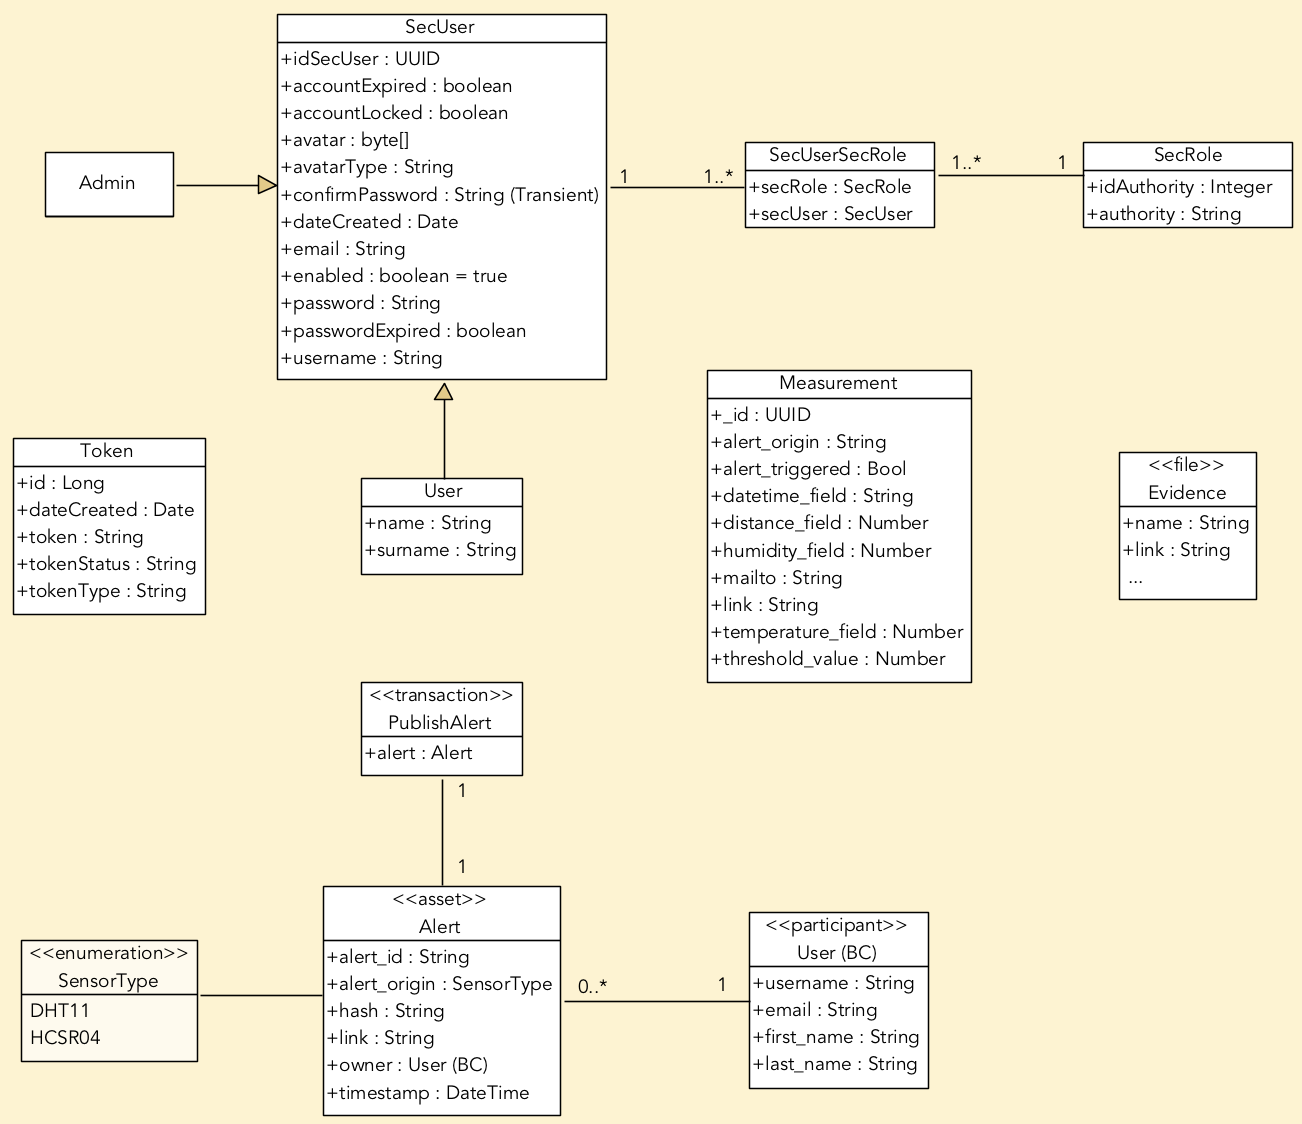
\includegraphics[width=17cm,height=14cm]{Images/analysis/classDiagram} \\
			\label{fig:domain_model} 
		\end{center}  
	\end{figure}  
	
	% Section
	\section{Diagramas de secuencia de análisis}
		
	En esta sección se muestran los diagramas de secuencia de análisis que representan las interacciones de las entidades del sistema con los casos de uso, ambos detallados en puntos anteriores.
			
	\begin{itemize}
		\item Diagrama de secuencia de análisis: Configurar dispositivo \gls{raspberry-a} (Figura \ref{fig:ds_configurarRPi1} - Parte 1 y Figura \ref{fig:ds_configurarRPi2} - Parte 2).
		
		\begin{figure}[!ht]   
			\caption{Diagrama de secuencia de análisis: Configurar dispositivo RPi - Parte 1.} 
			\begin{center} 
	 			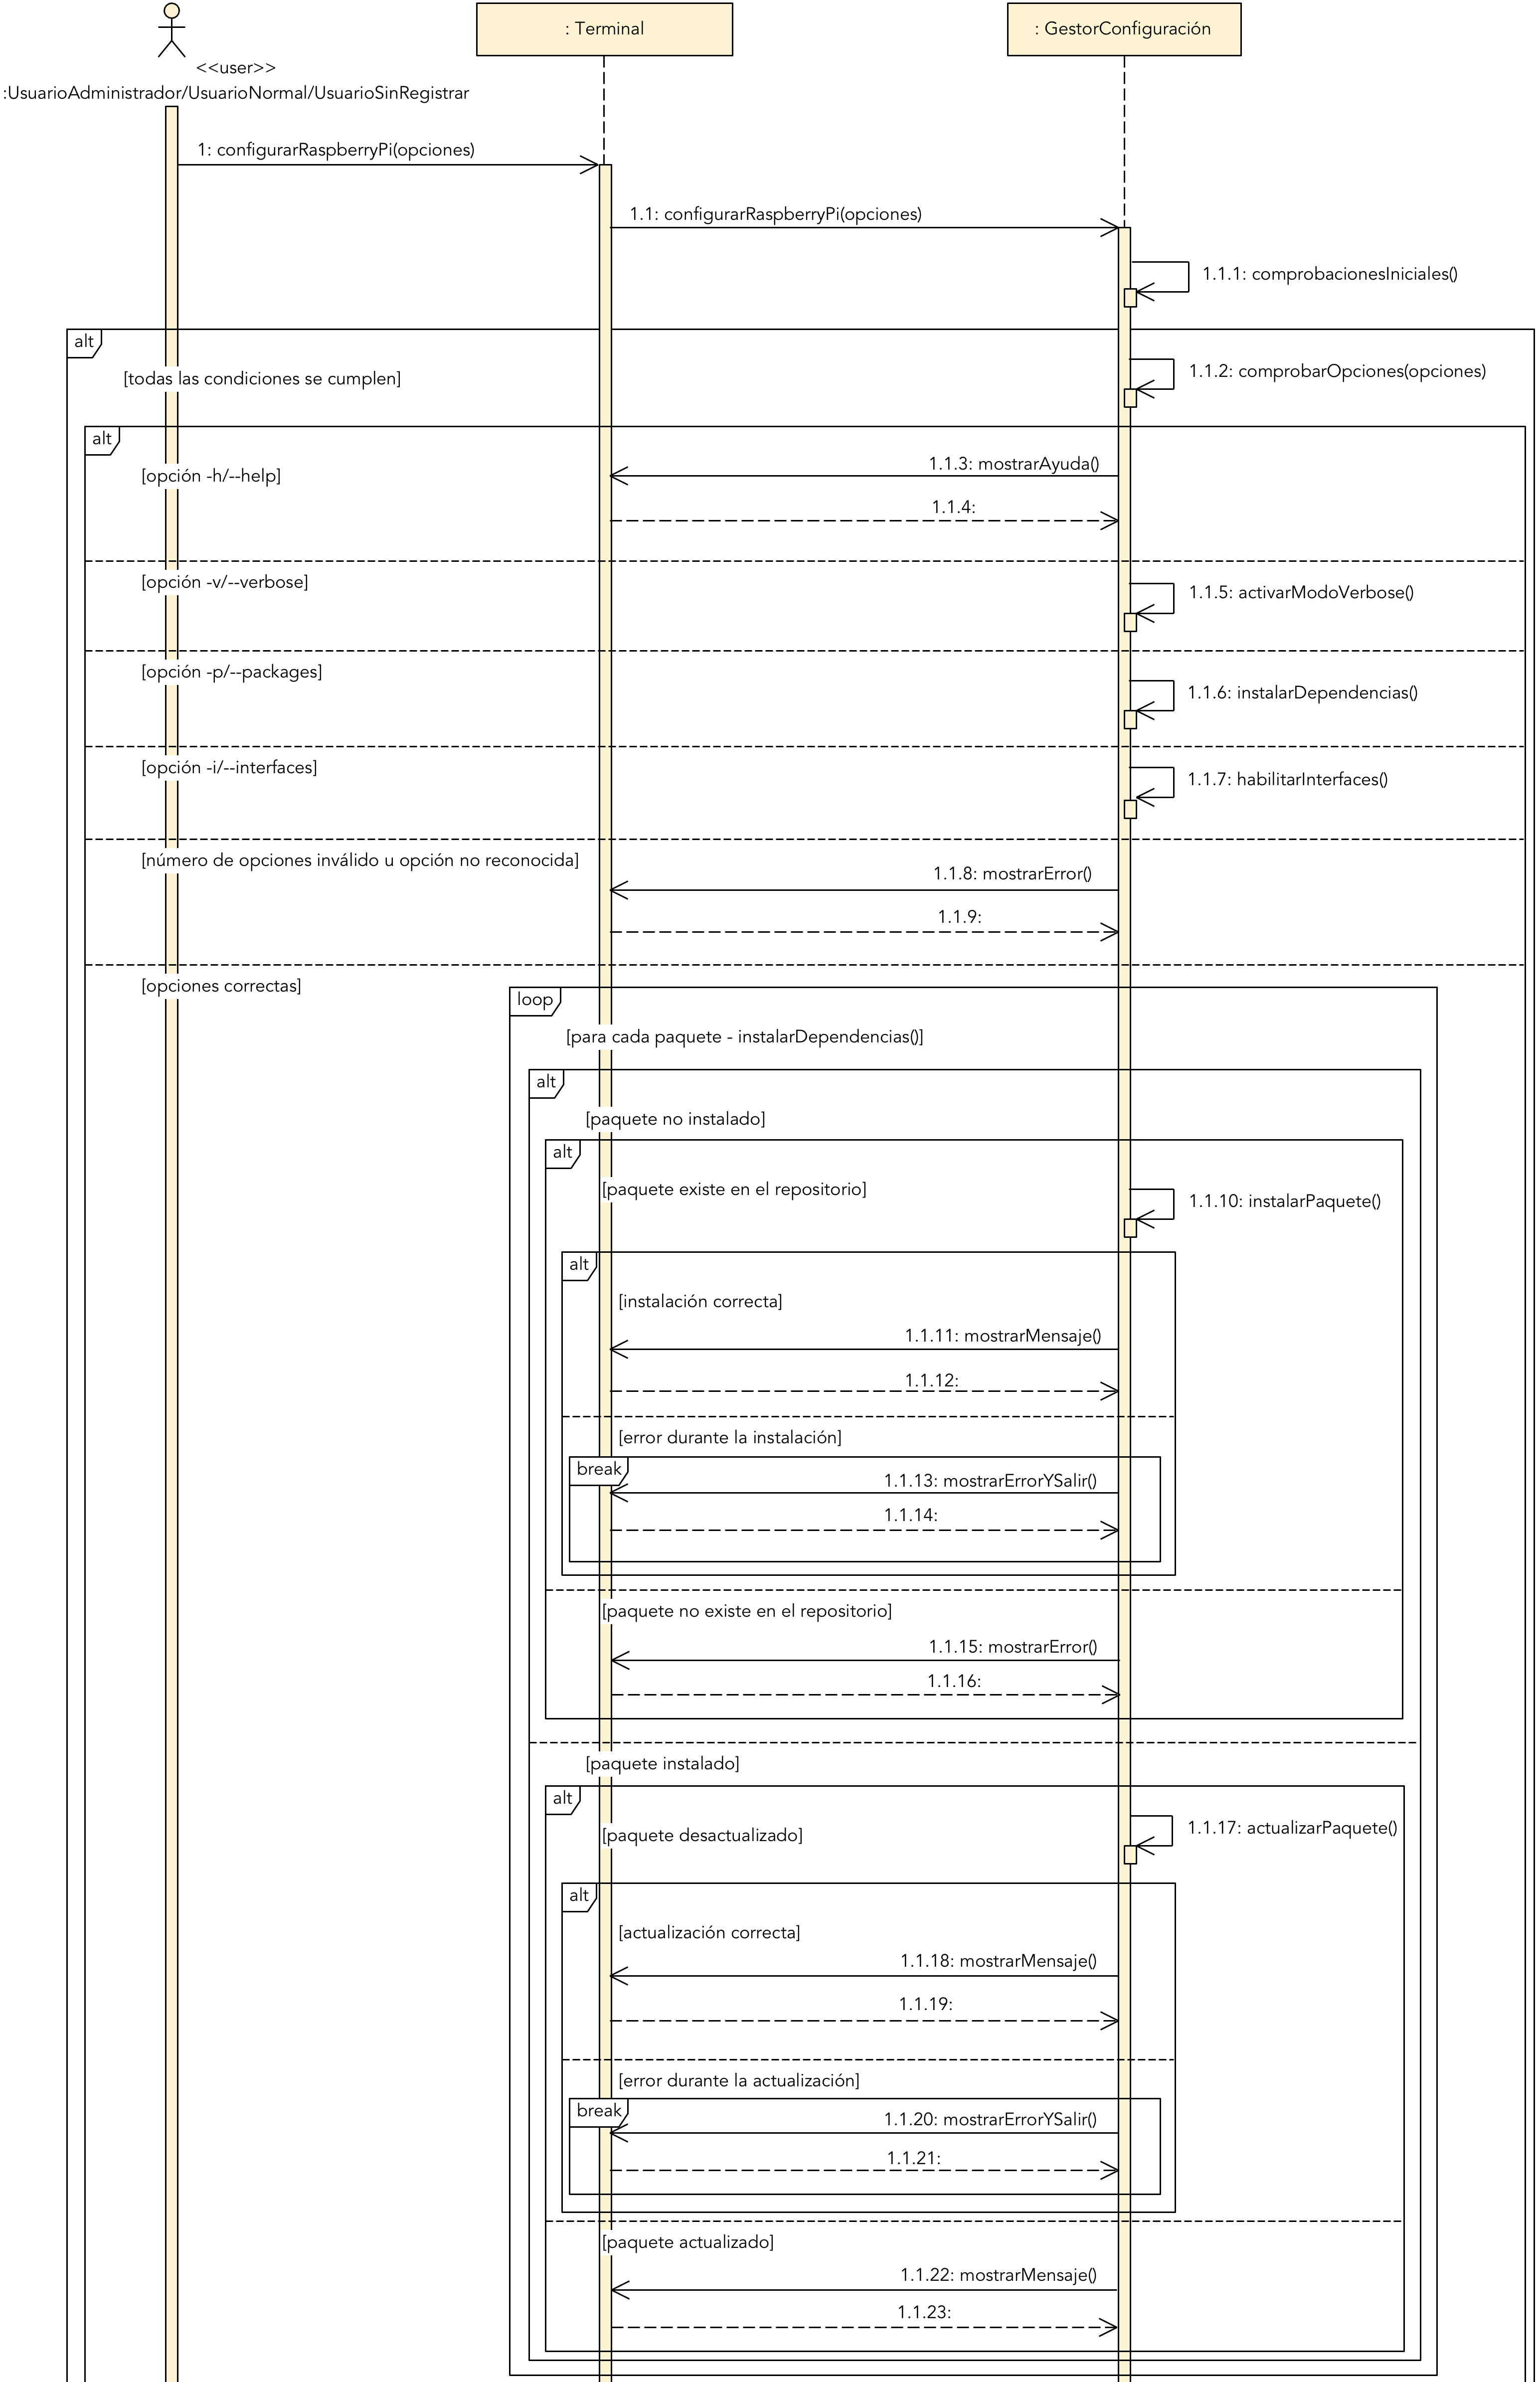
\includegraphics[width=17cm,height=17cm]{Images/analysis/secuencia/secuencia_configurarRPi_parte1} \\
				\label{fig:ds_configurarRPi1} 
			\end{center}  
		\end{figure} 
		
		\begin{figure}[!ht]   
			\caption{Diagrama de secuencia de análisis: Configurar dispositivo RPi - Parte 2.} 
			\begin{center} 
	 			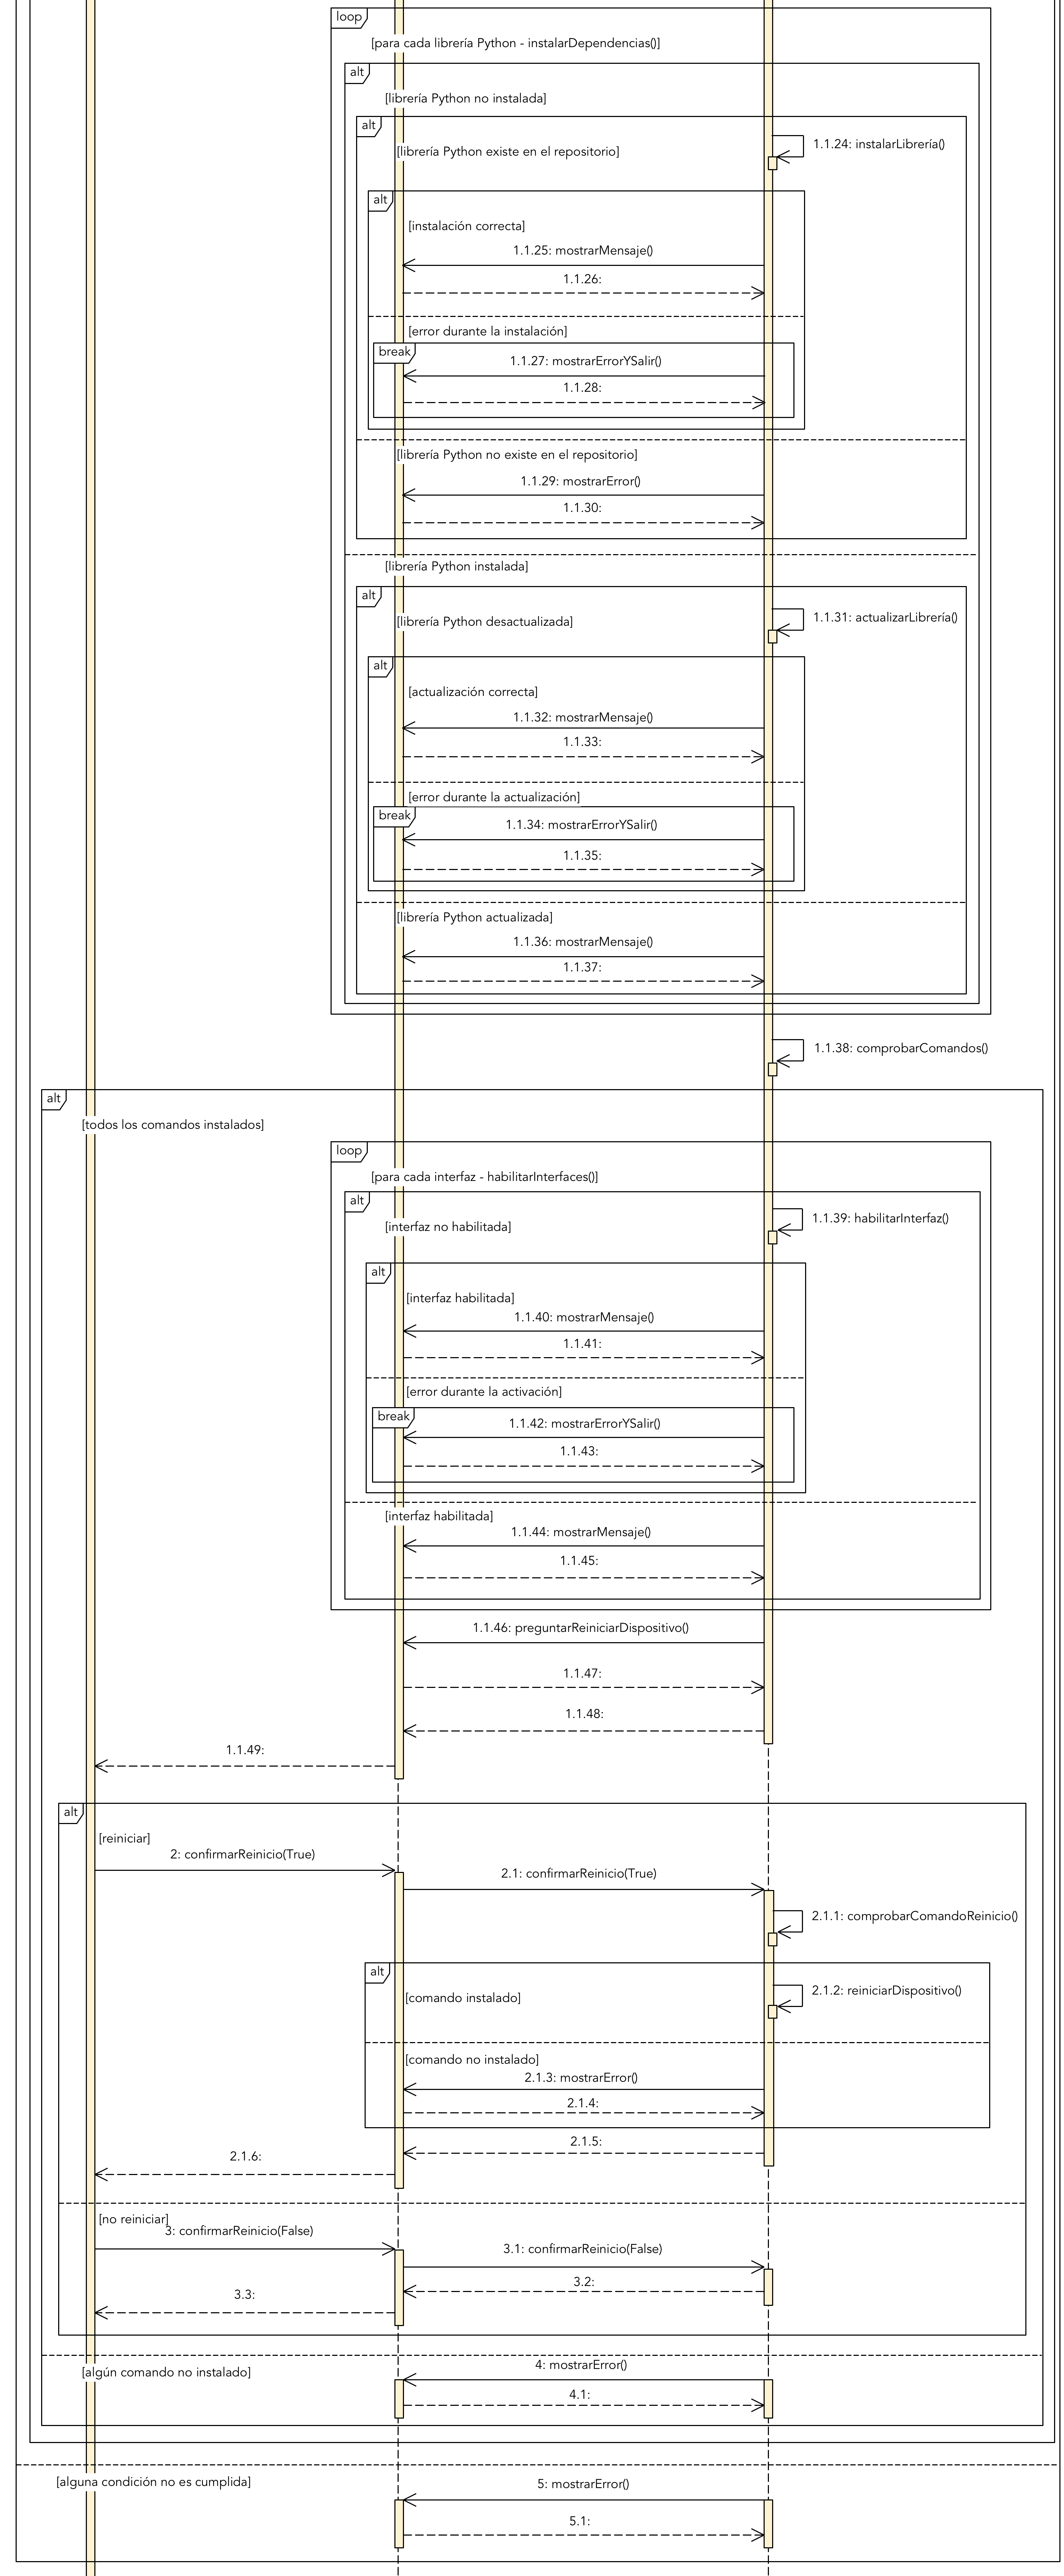
\includegraphics[width=17cm,height=21cm]{Images/analysis/secuencia/secuencia_configurarRPi_parte2} \\
				\label{fig:ds_configurarRPi2} 
			\end{center}  
		\end{figure} 
		
		% NEW PAGE 
		\newpage
		 
		\item Diagrama de secuencia de análisis: Monitorizar sucesos del entorno (Figura \ref{fig:ds_monitorizarEntorno}).
		
		\begin{figure}[!ht]   
			\caption{Diagrama de secuencia de análisis: Monitorizar sucesos del entorno.} 
			\begin{center} 
				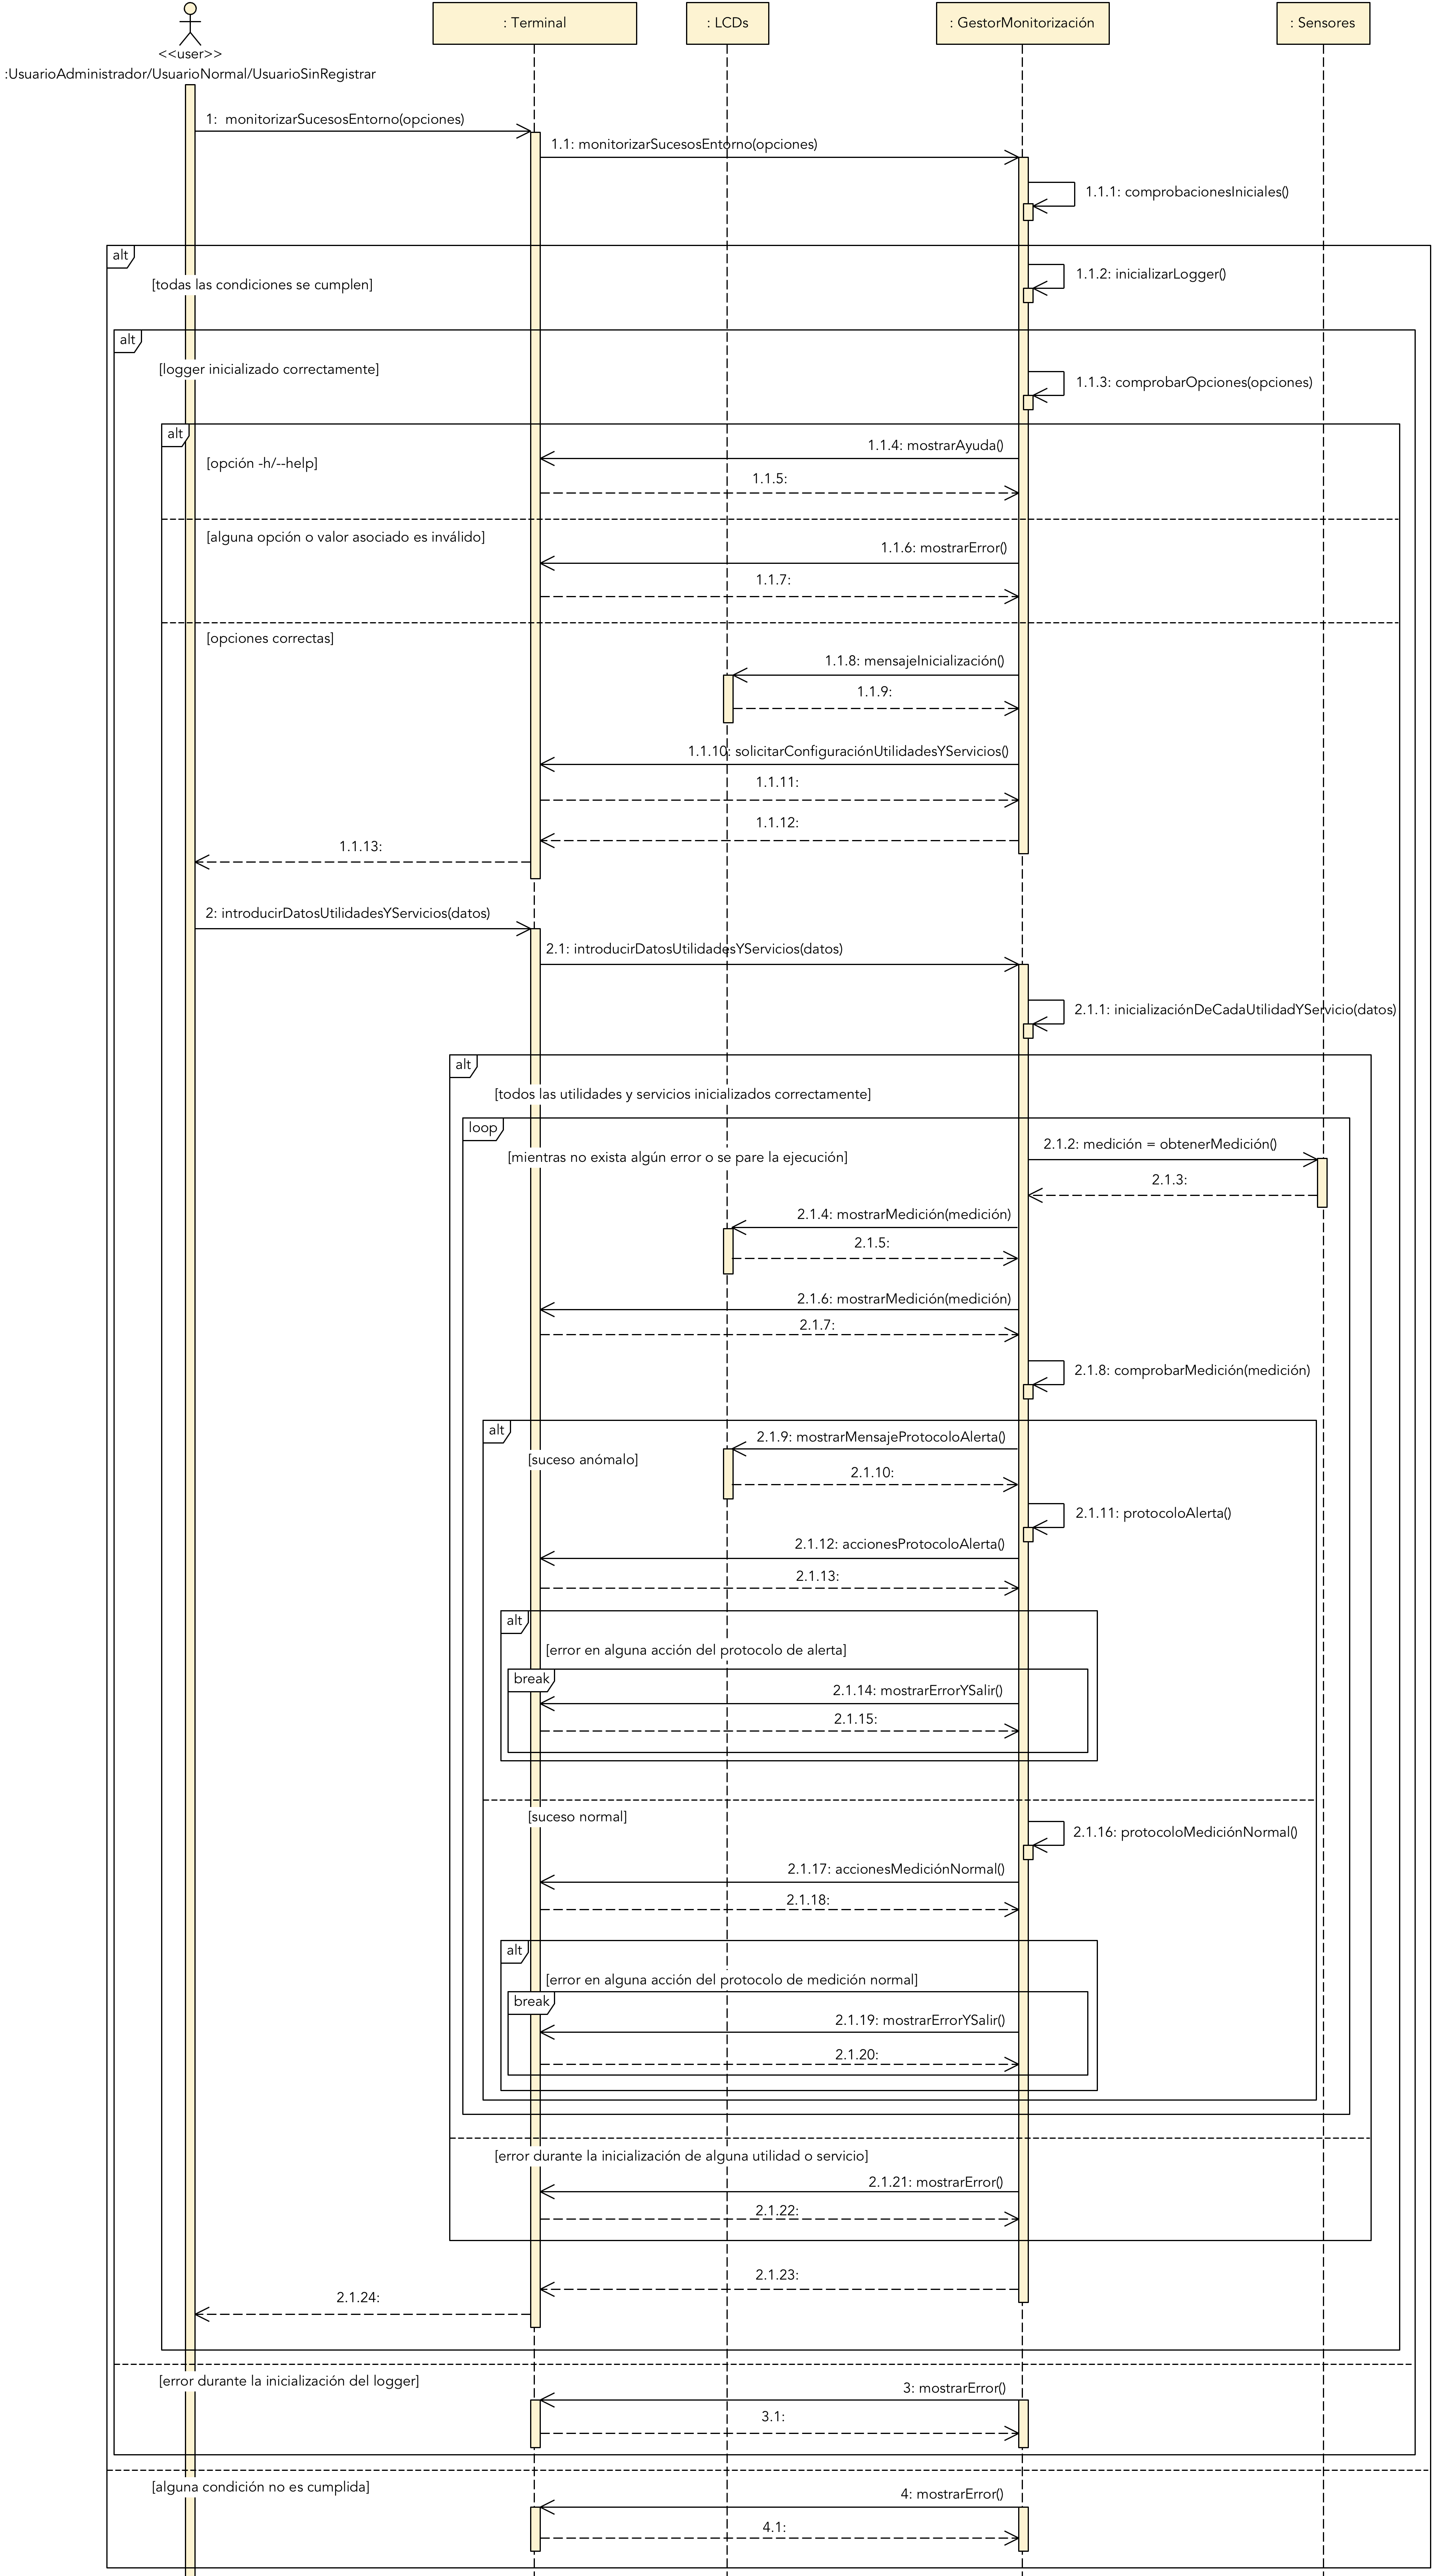
\includegraphics[width=17cm,height=20.5cm]{Images/analysis/secuencia/secuencia_monitorizarEntorno} \\
				\label{fig:ds_monitorizarEntorno} 
			\end{center}  
		\end{figure} 

		% NEW PAGE 
		\newpage
		
		\item Diagrama de secuencia de análisis: Desencriptar evidencia (Figura \ref{fig:ds_desencriptar}).

		\begin{figure}[!ht]   
			\caption{Diagrama de secuencia de análisis: Desencriptar evidencia.} 
			\begin{center} 
	 			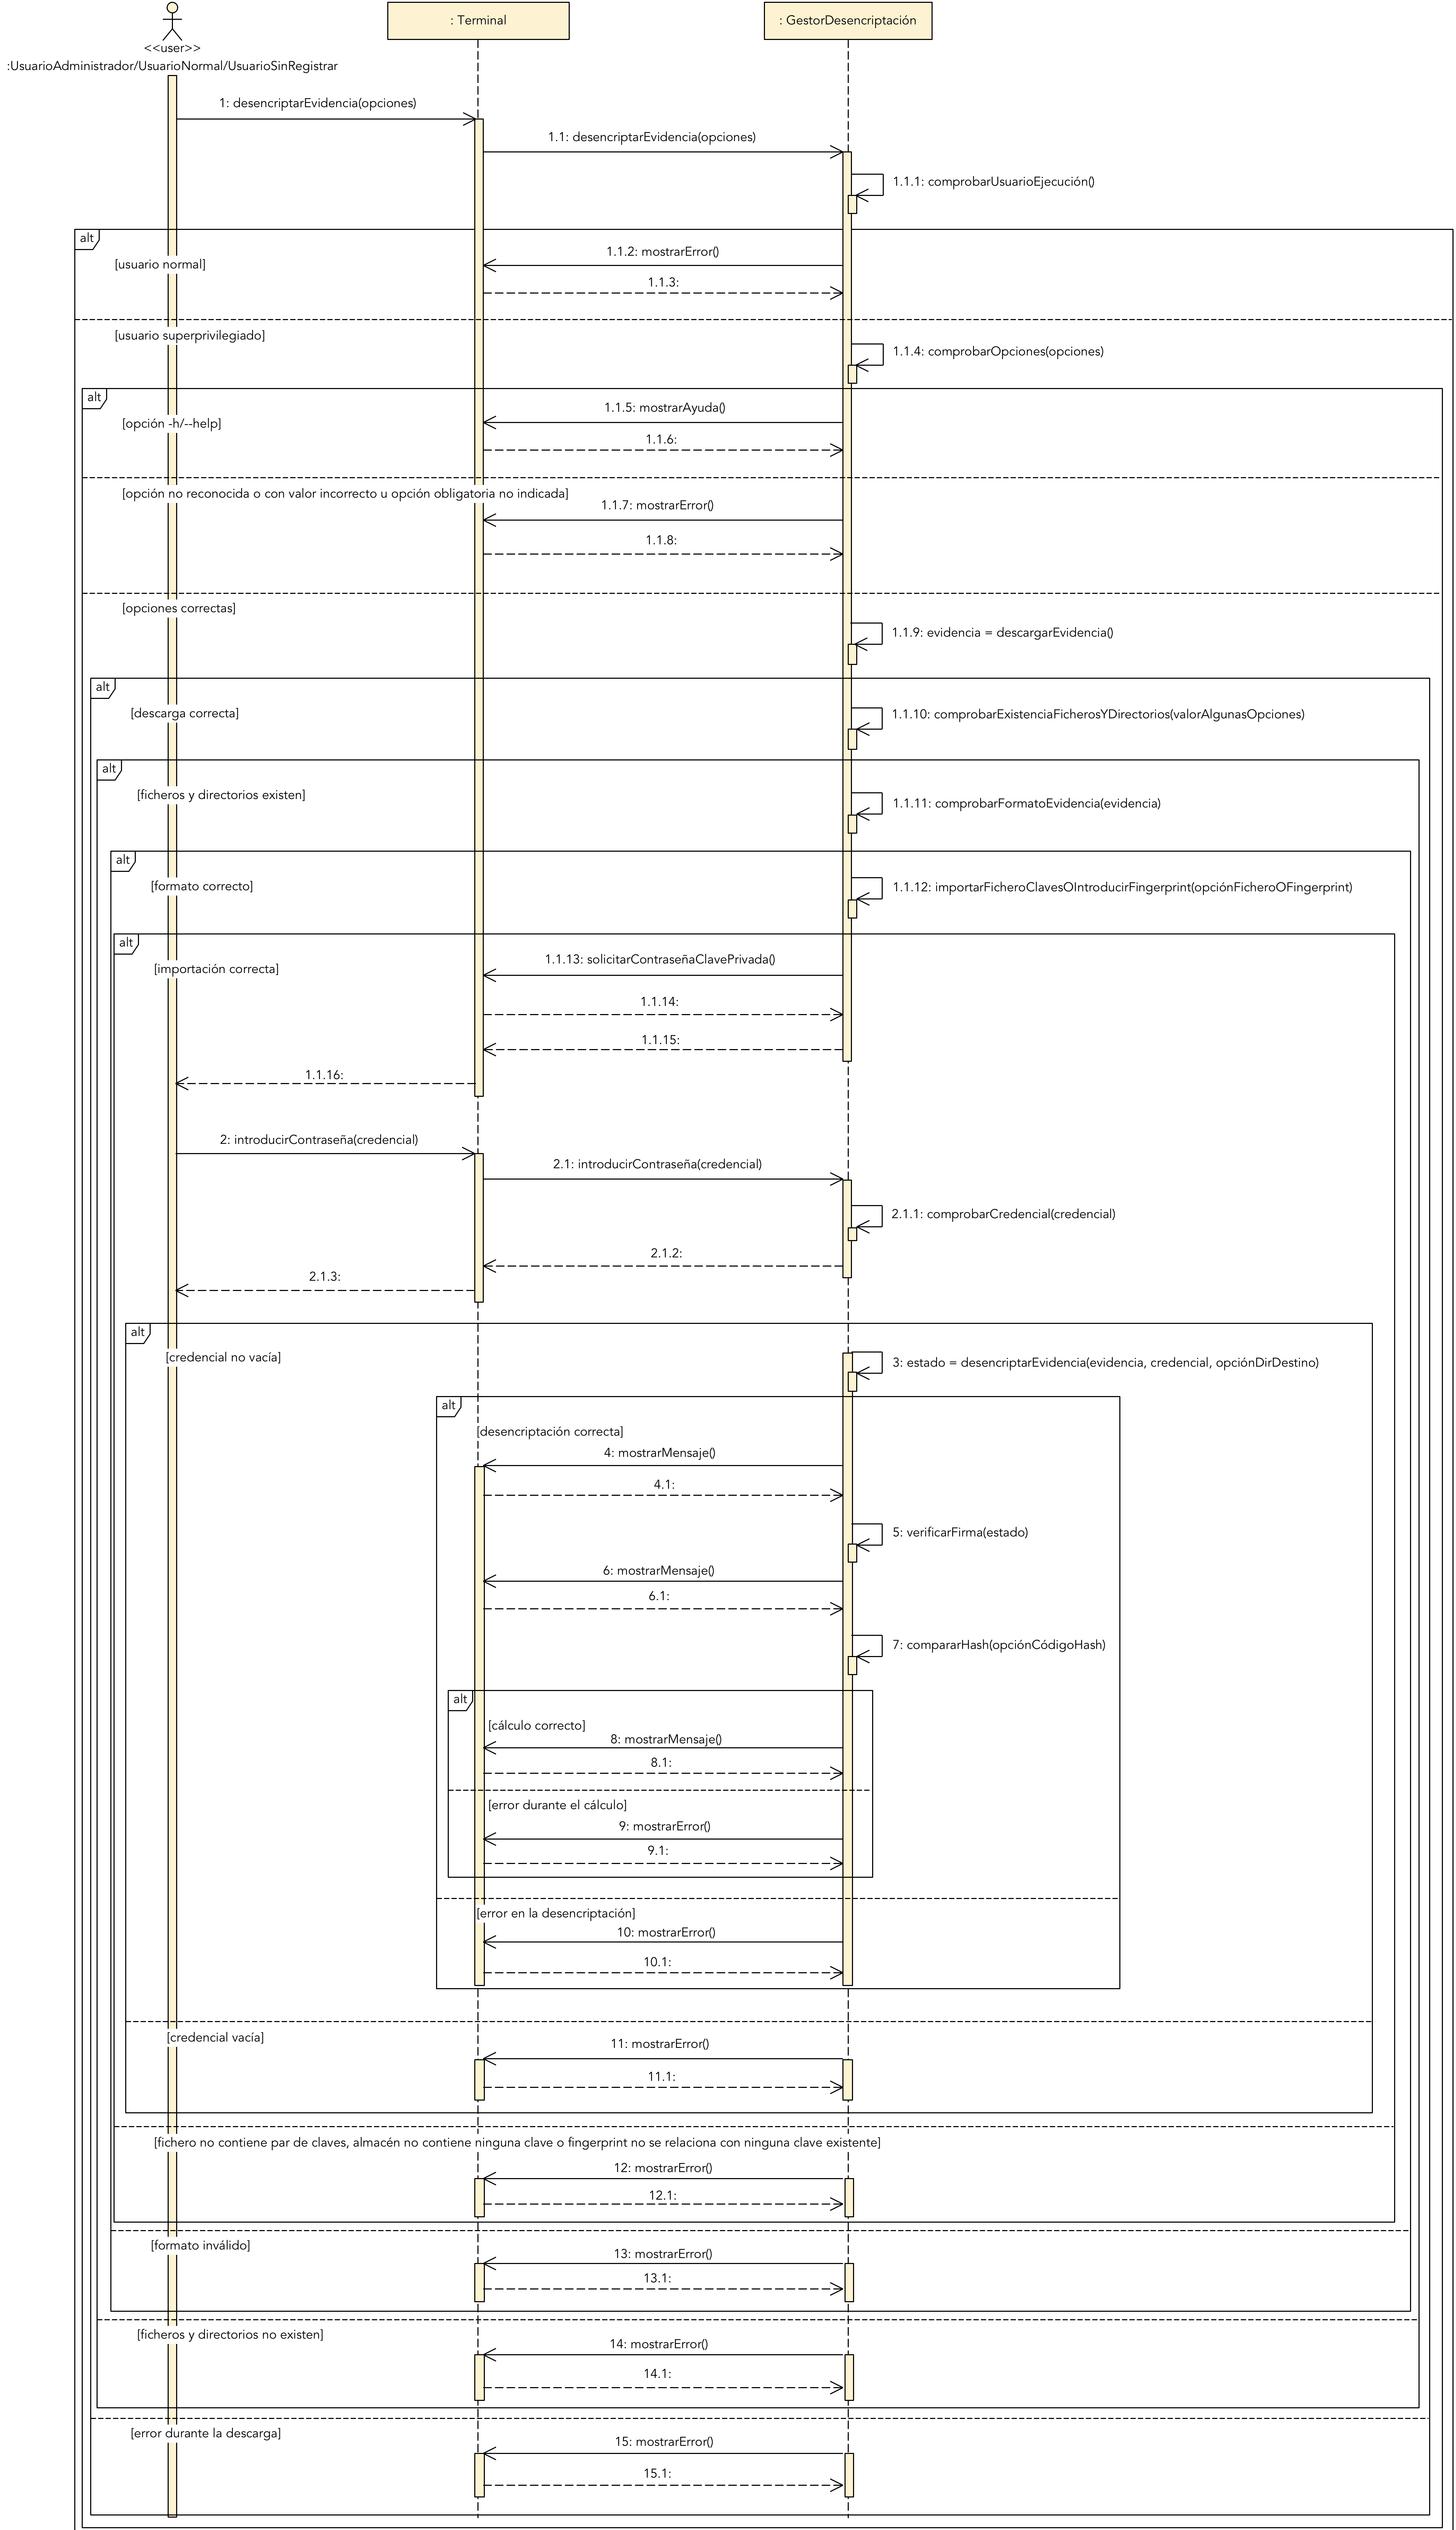
\includegraphics[width=17cm,height=20.5cm]{Images/analysis/secuencia/secuencia_desencriptarEvidencia} \\
				\label{fig:ds_desencriptar} 
			\end{center}  
		\end{figure} 
		
		% NEW PAGE 
		\newpage
		
		\item Diagrama de secuencia de análisis: Iniciar sesión (Figura \ref{fig:ds_iniciarSesion}).
		
		\begin{figure}[!ht]   
			\caption{Diagrama de secuencia de análisis: Iniciar sesión.} 
			\begin{center} 
	 			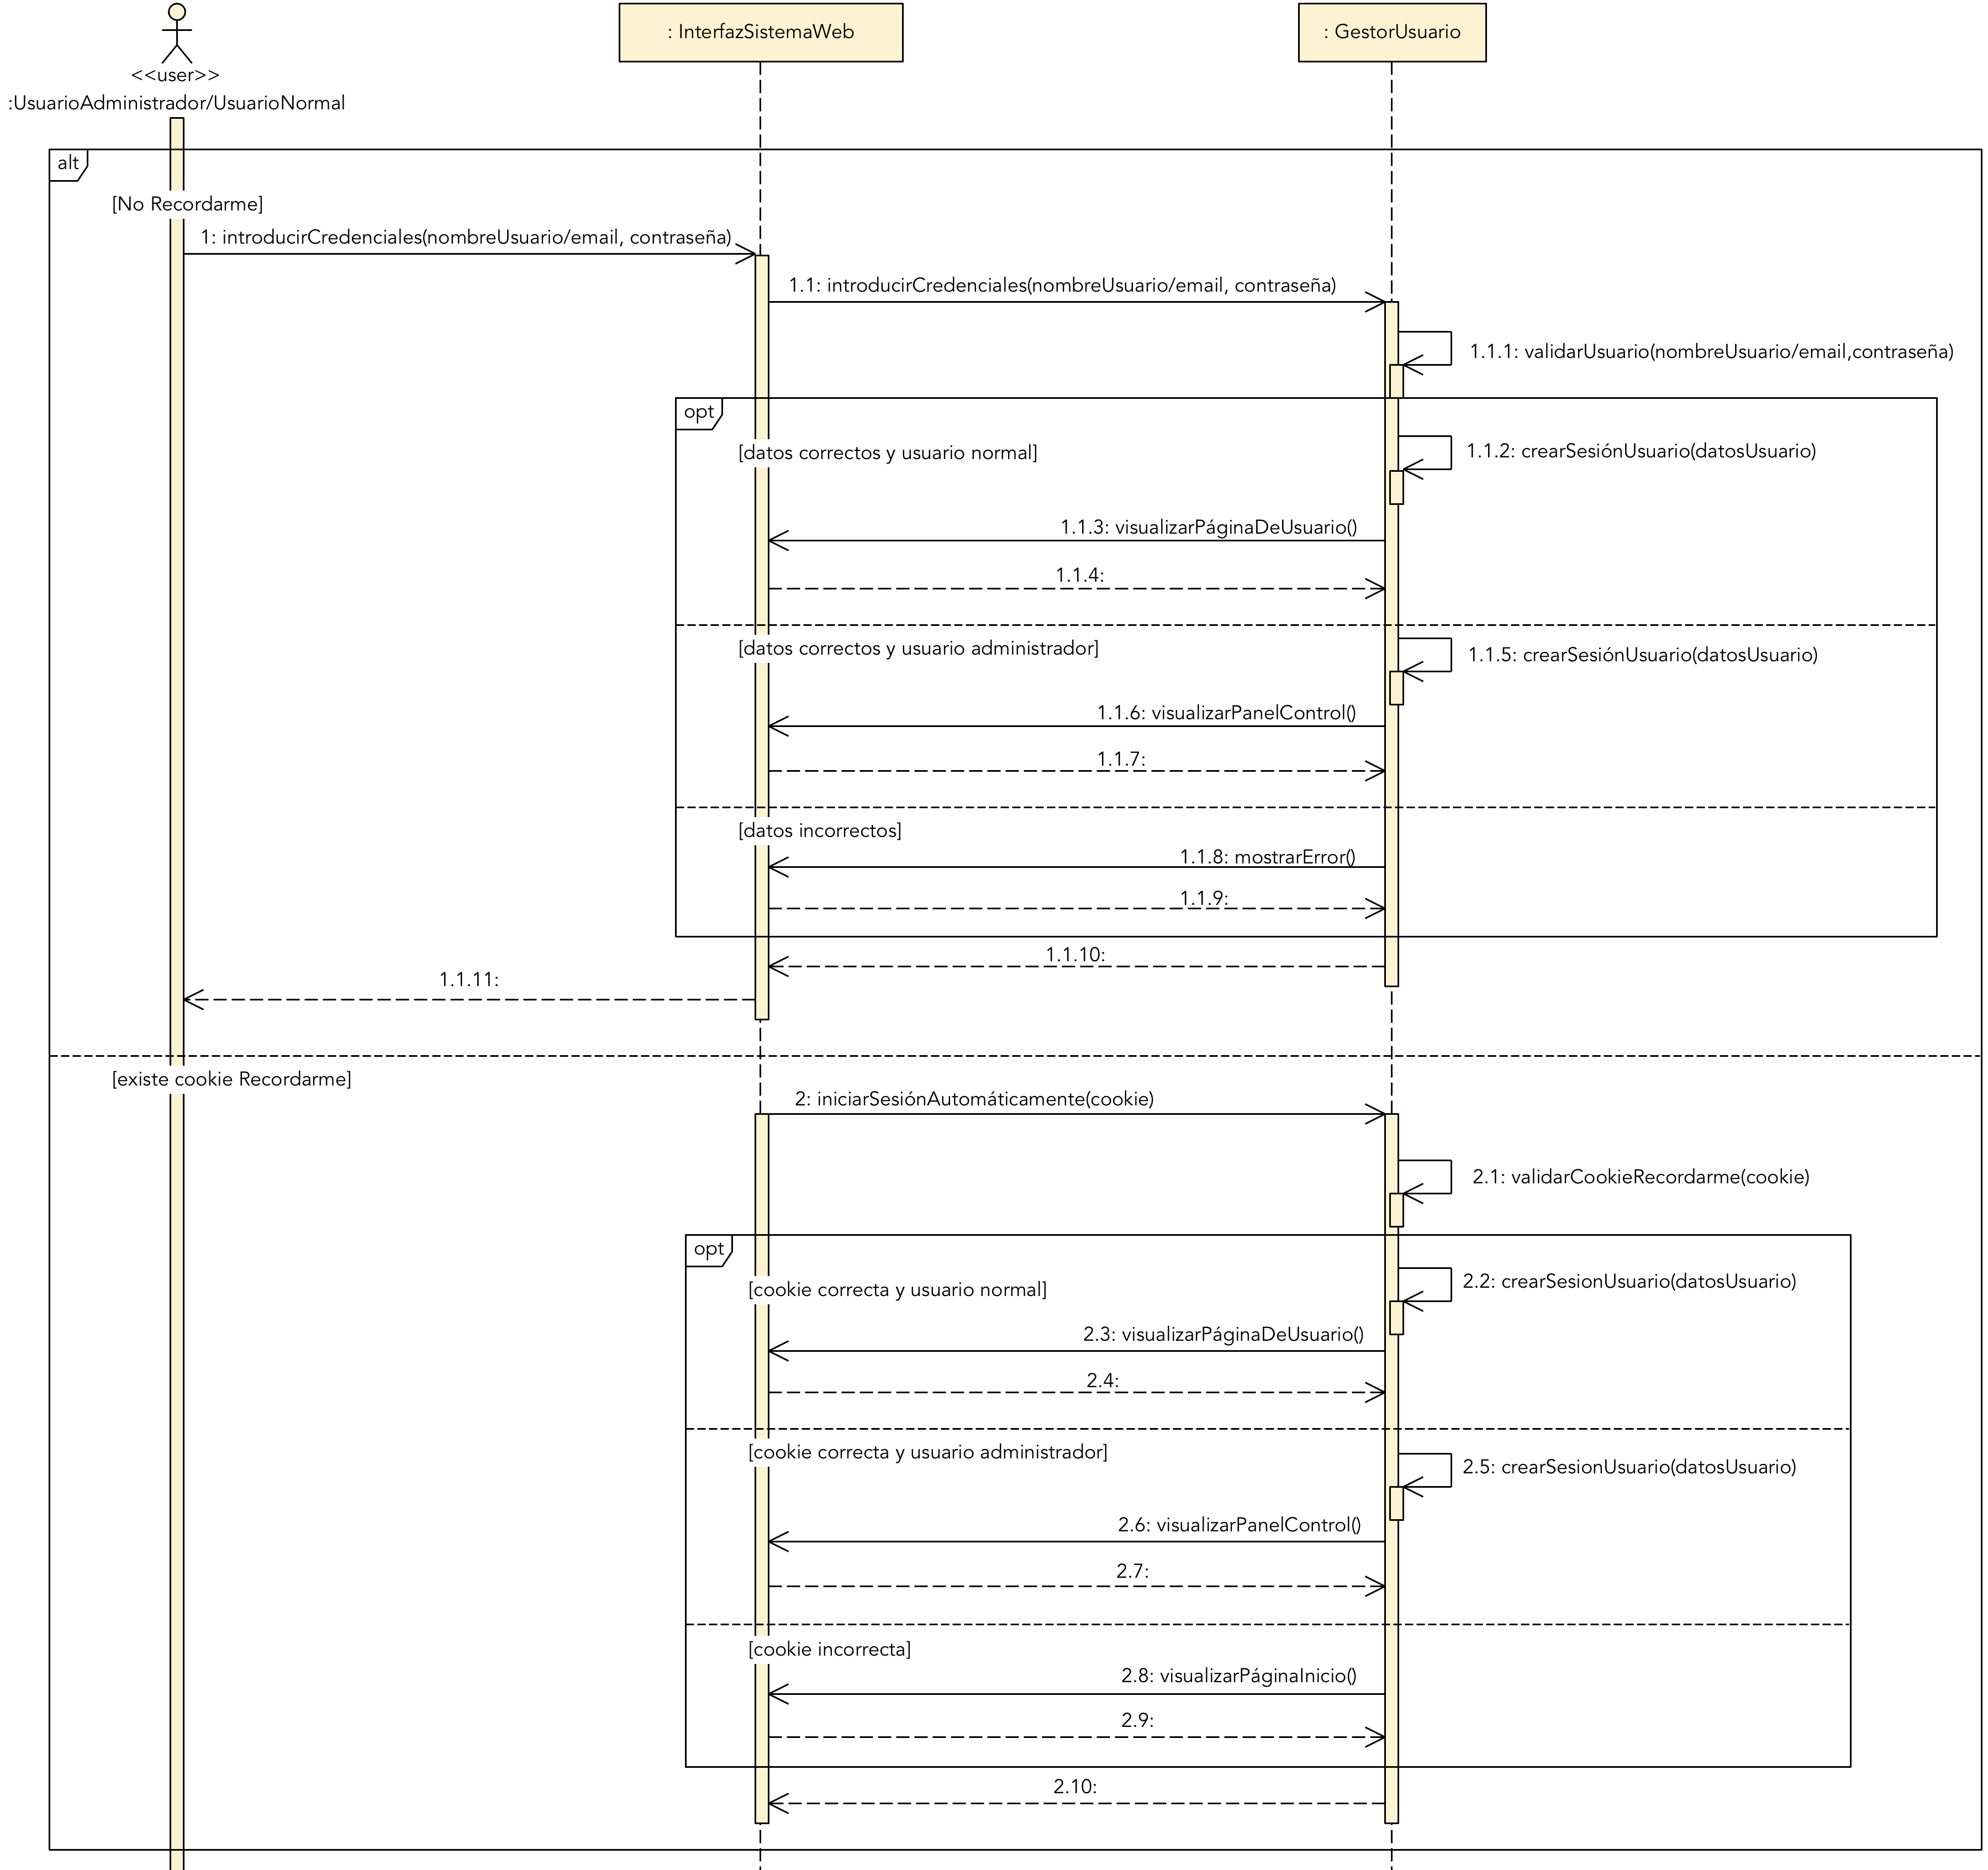
\includegraphics[width=17cm,height=20cm]{Images/analysis/secuencia/secuencia_iniciarSesion} \\
				\label{fig:ds_iniciarSesion} 
			\end{center}  
		\end{figure} 
		
		% NEW PAGE 
		\newpage
		
		\item Diagrama de secuencia de análisis: Gestionar usuario administrador (Figura \ref{fig:ds_adminuser1} - Parte 1 y Figura \ref{fig:ds_adminuser2} - Parte 2)\footnote{El diagrama de secuencia de análisis para el caso de uso UC-0007: Gestionar usuario normal es similar al presente con la salvedad de adaptar a la entidad correspondiente.}.
		 
		\begin{figure}[!ht]   
			\caption{Diagrama de secuencia de análisis: Gestionar usuario administrador - Parte 1.} 
			\begin{center} 
	 			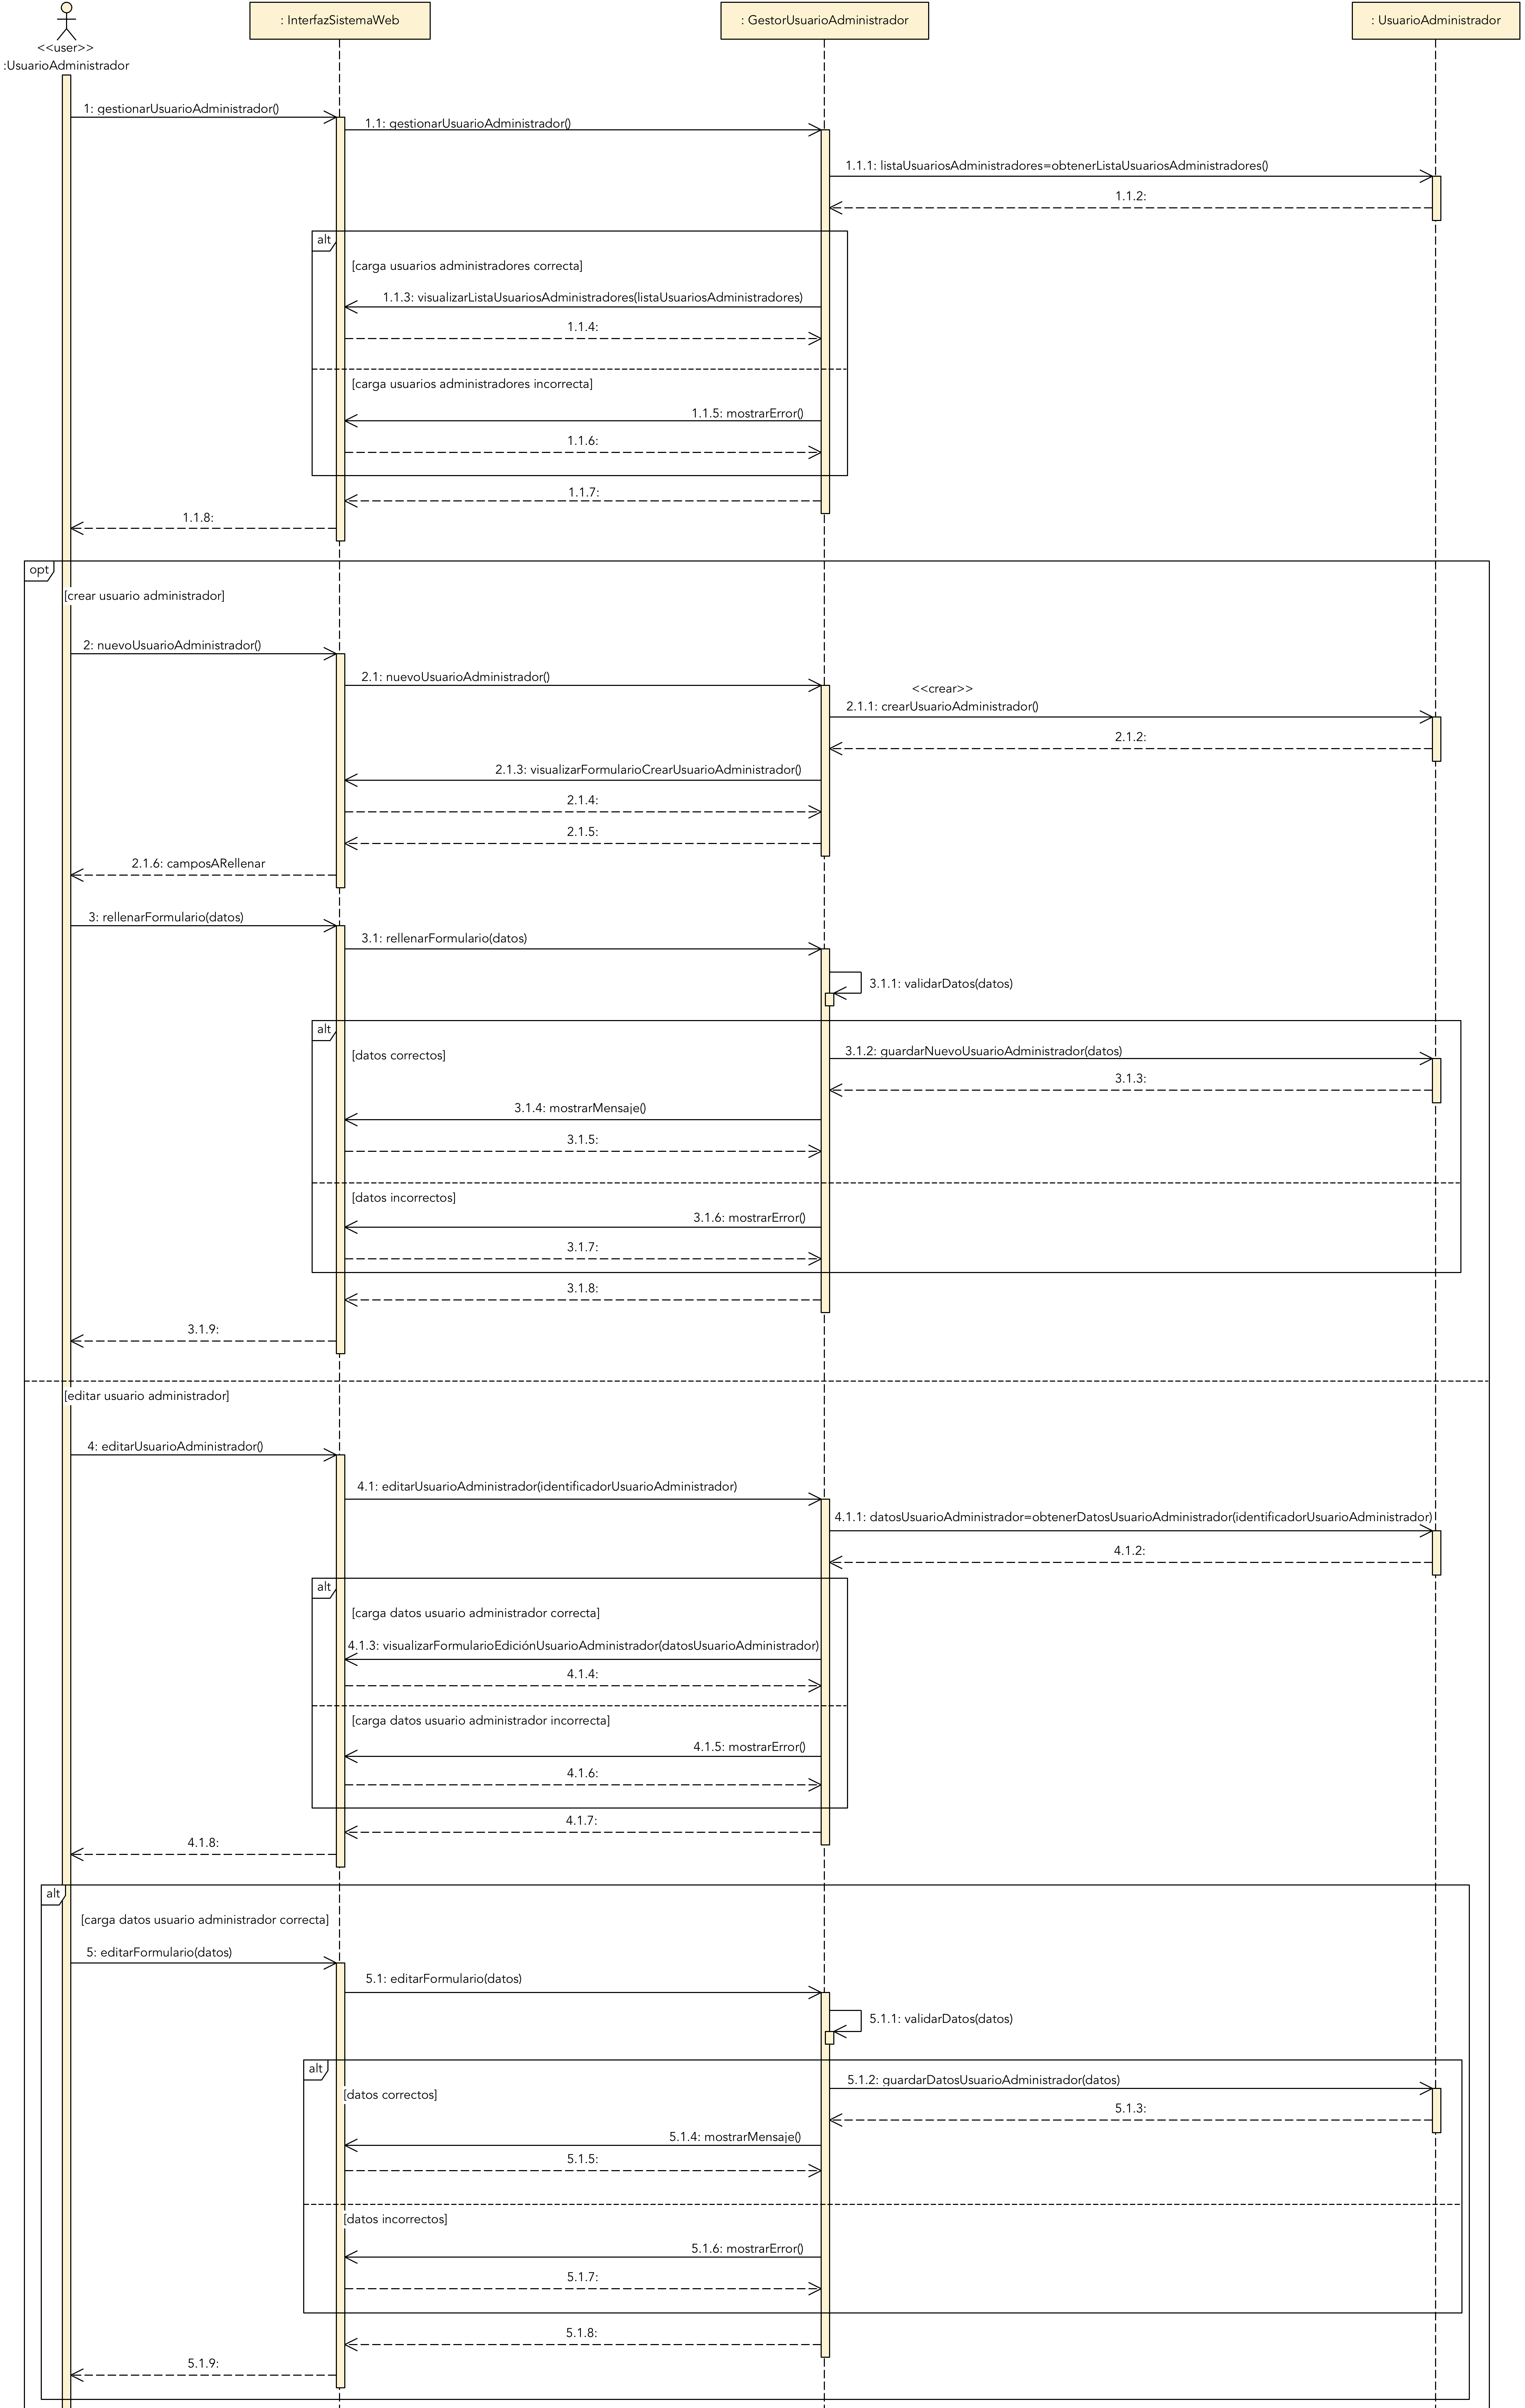
\includegraphics[width=17cm,height=18.5cm]{Images/analysis/secuencia/secuencia_gestionarUsuarioAdministrador_parte1} \\
				\label{fig:ds_adminuser1} 
			\end{center}  
		\end{figure} 
		
		% NEW PAGE
		\newpage
		
		\begin{figure}[!ht]   
			\caption{Diagrama de secuencia de análisis: Gestionar usuario administrador - Parte 2.} 
			\begin{center} 
	 			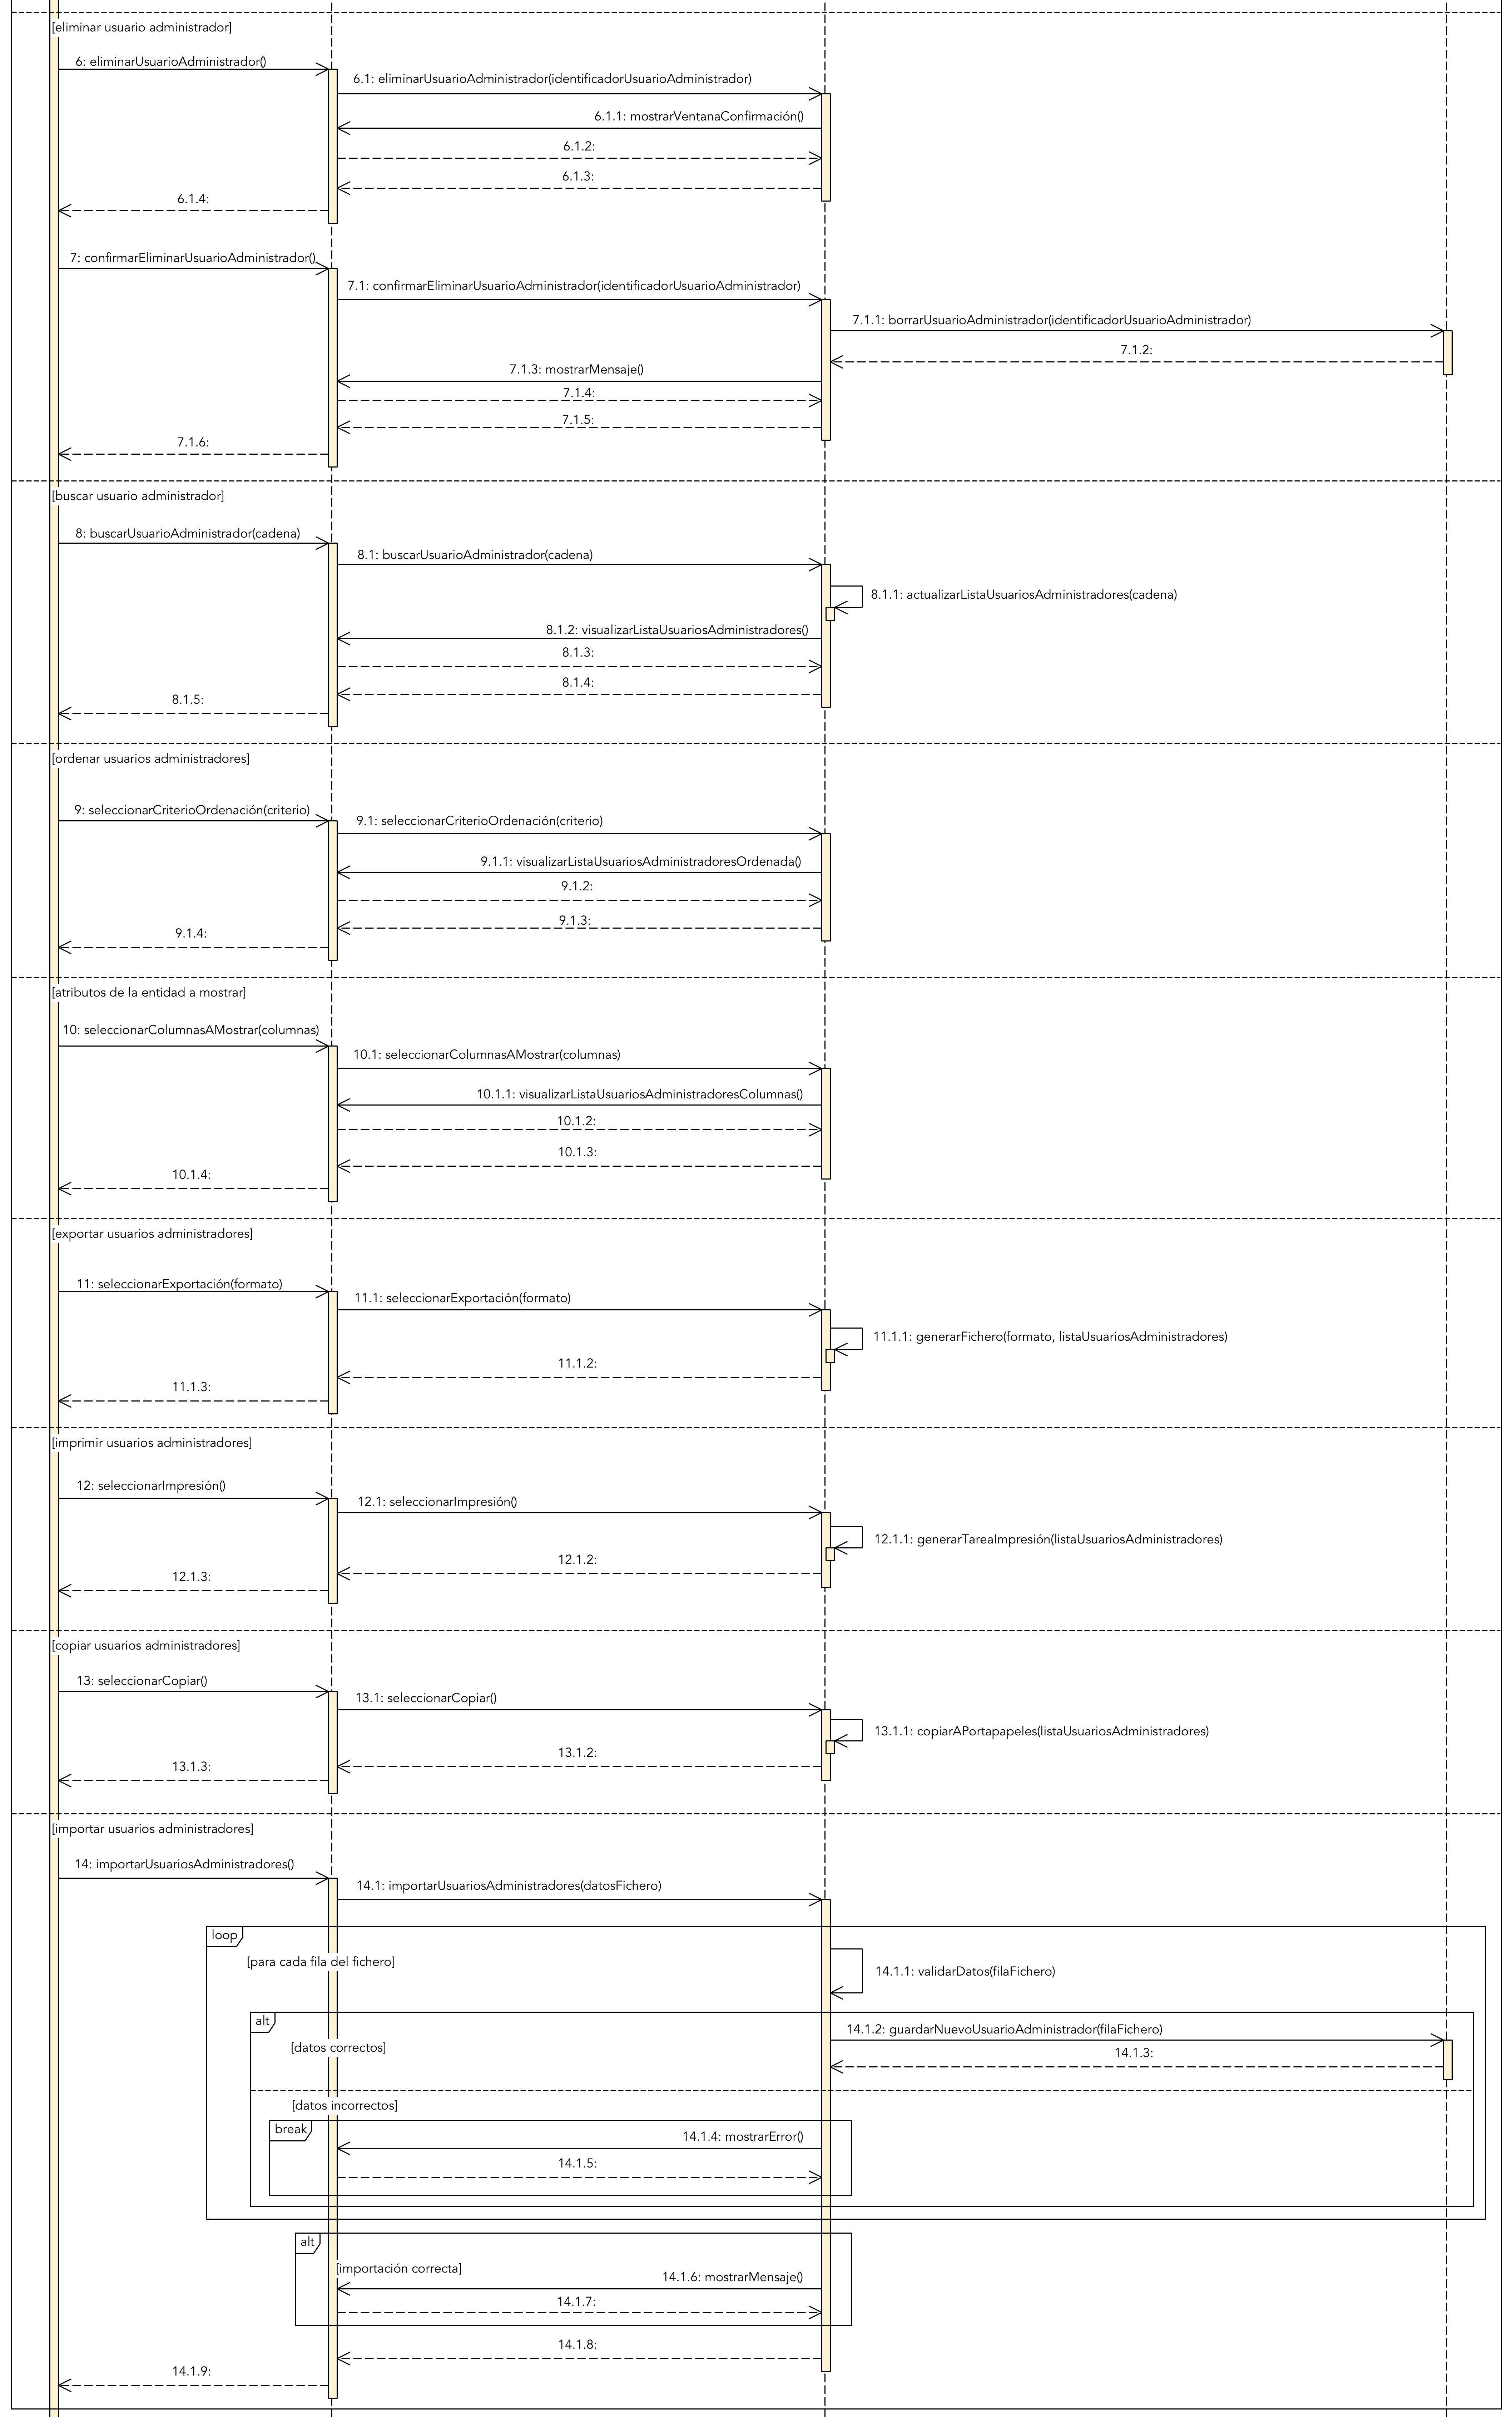
\includegraphics[width=17cm,height=21cm]{Images/analysis/secuencia/secuencia_gestionarUsuarioAdministrador_parte2} \\
				\label{fig:ds_adminuser2} 
			\end{center}  
		\end{figure} 
		
		% NEW PAGE 
		\newpage
		
		\item Diagrama de secuencia de análisis: Consultar estadísticas (Figura \ref{fig:ds_estadisticas}).
		
		\begin{figure}[!ht]   
			\caption{Diagrama de secuencia de análisis: Consultar estadísticas.} 
			\begin{center} 
	 			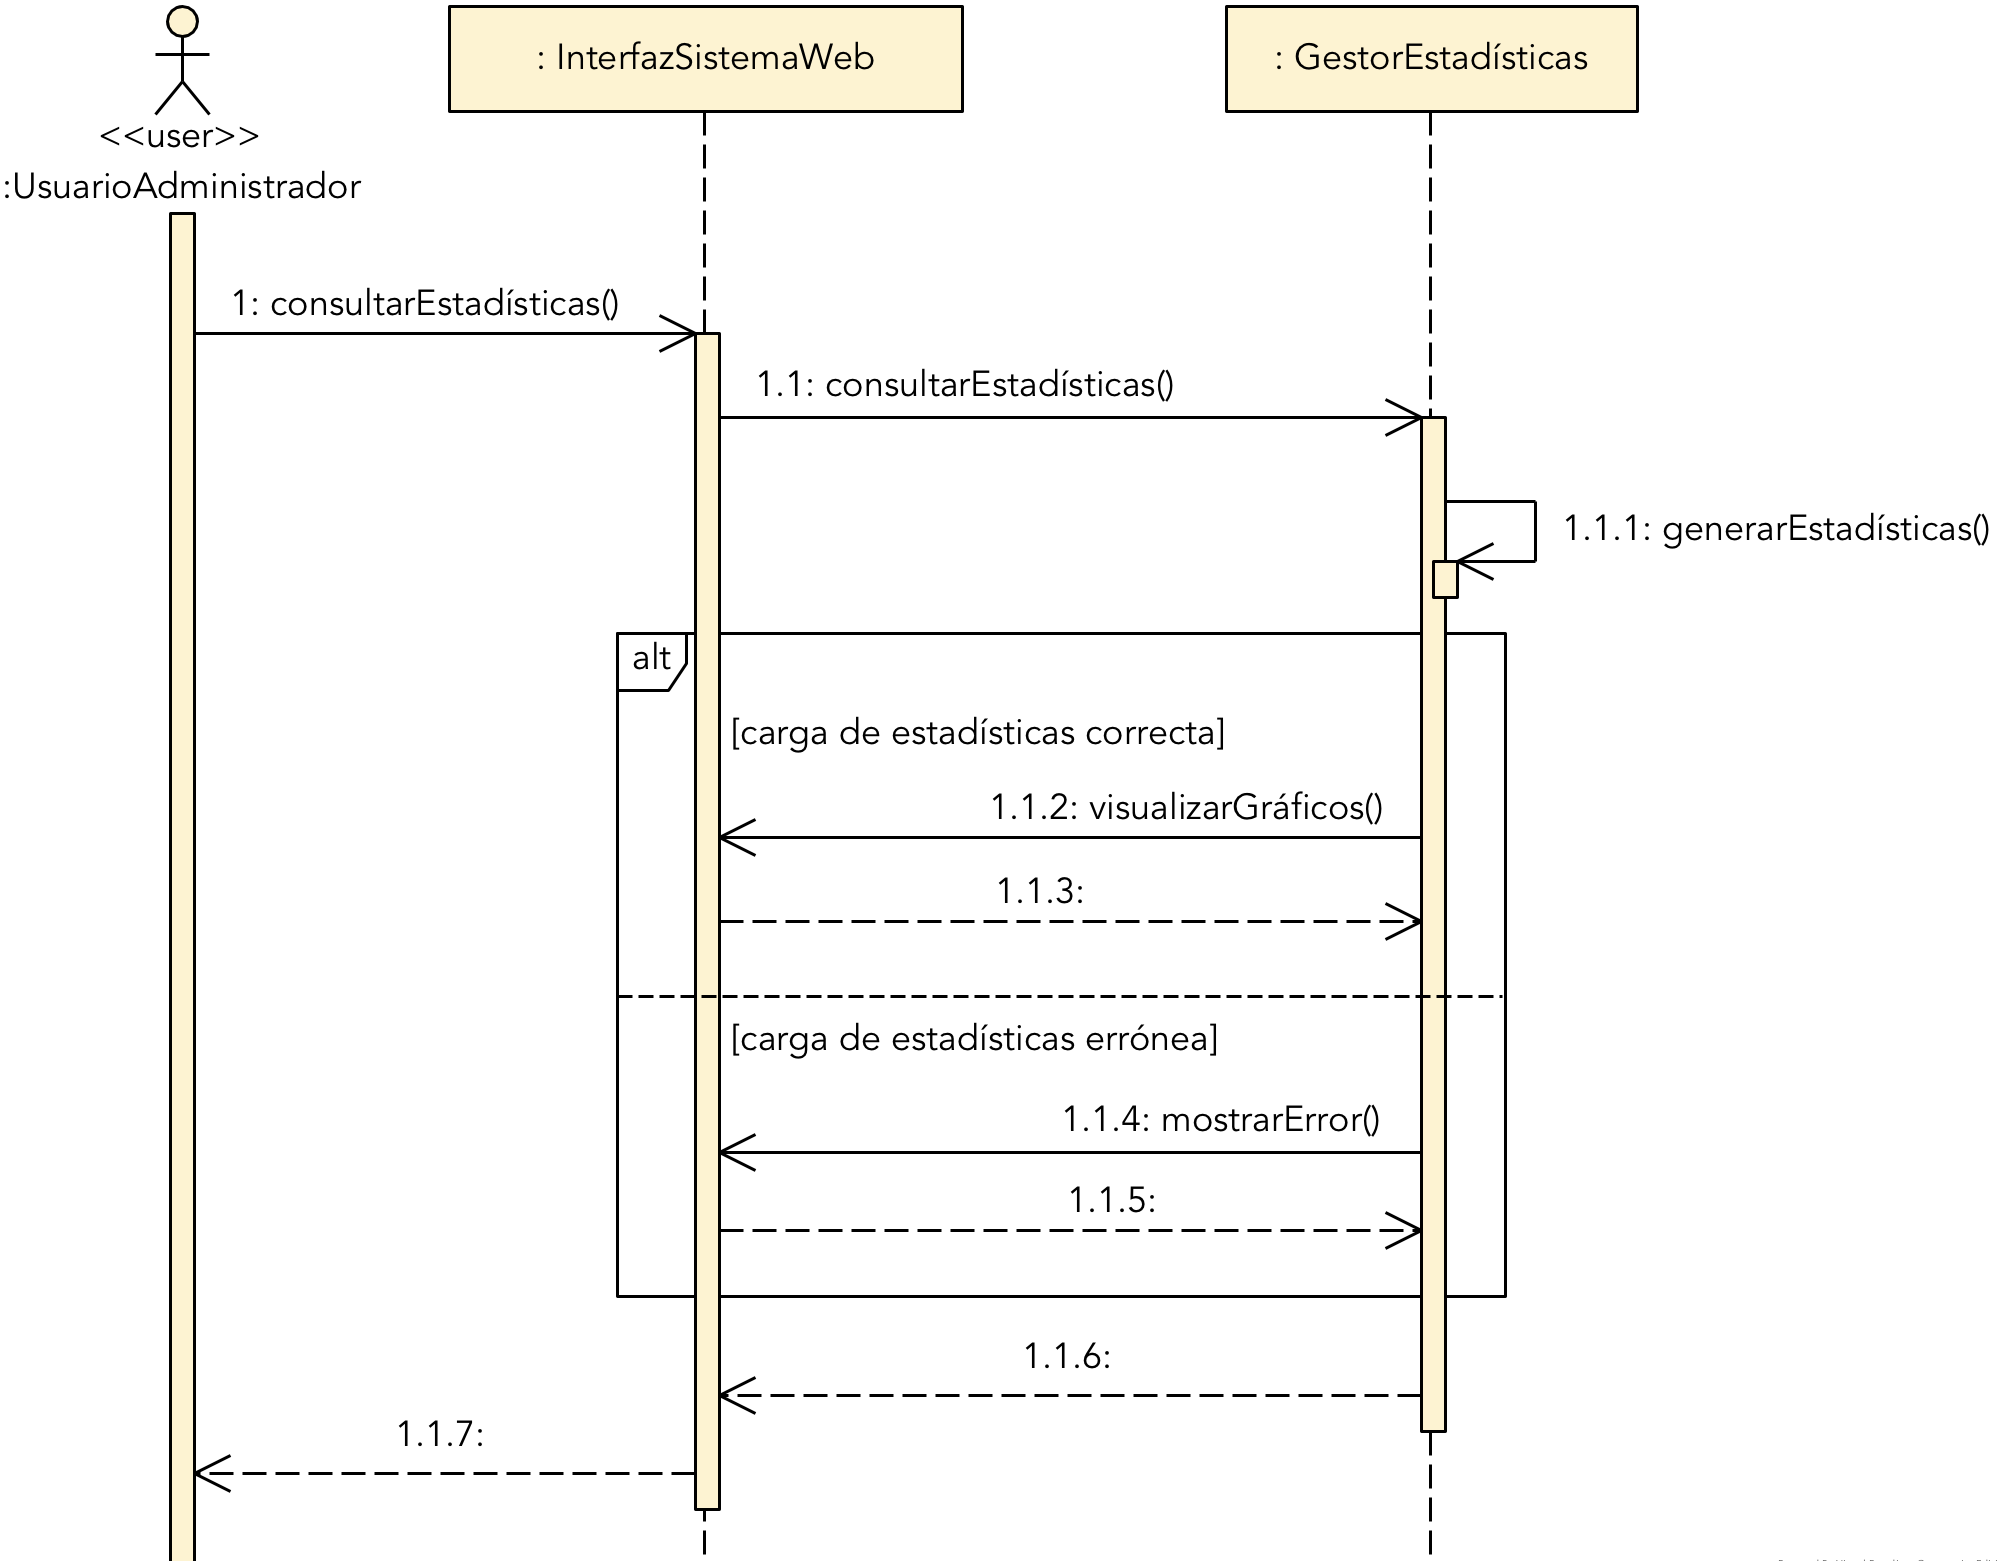
\includegraphics[width=17cm,height=13cm]{Images/analysis/secuencia/secuencia_consultarEstadisticas} \\
				\label{fig:ds_estadisticas} 
			\end{center}  
		\end{figure} 
		
		% NEW PAGE 
		\newpage
		
		\item Diagrama de secuencia de análisis: Consultar o modificar perfil personal (Figura \ref{fig:ds_perfil}).
		
		\begin{figure}[!ht]   
			\caption{Diagrama de secuencia de análisis: Consultar o modificar perfil personal.} 
			\begin{center} 
	 			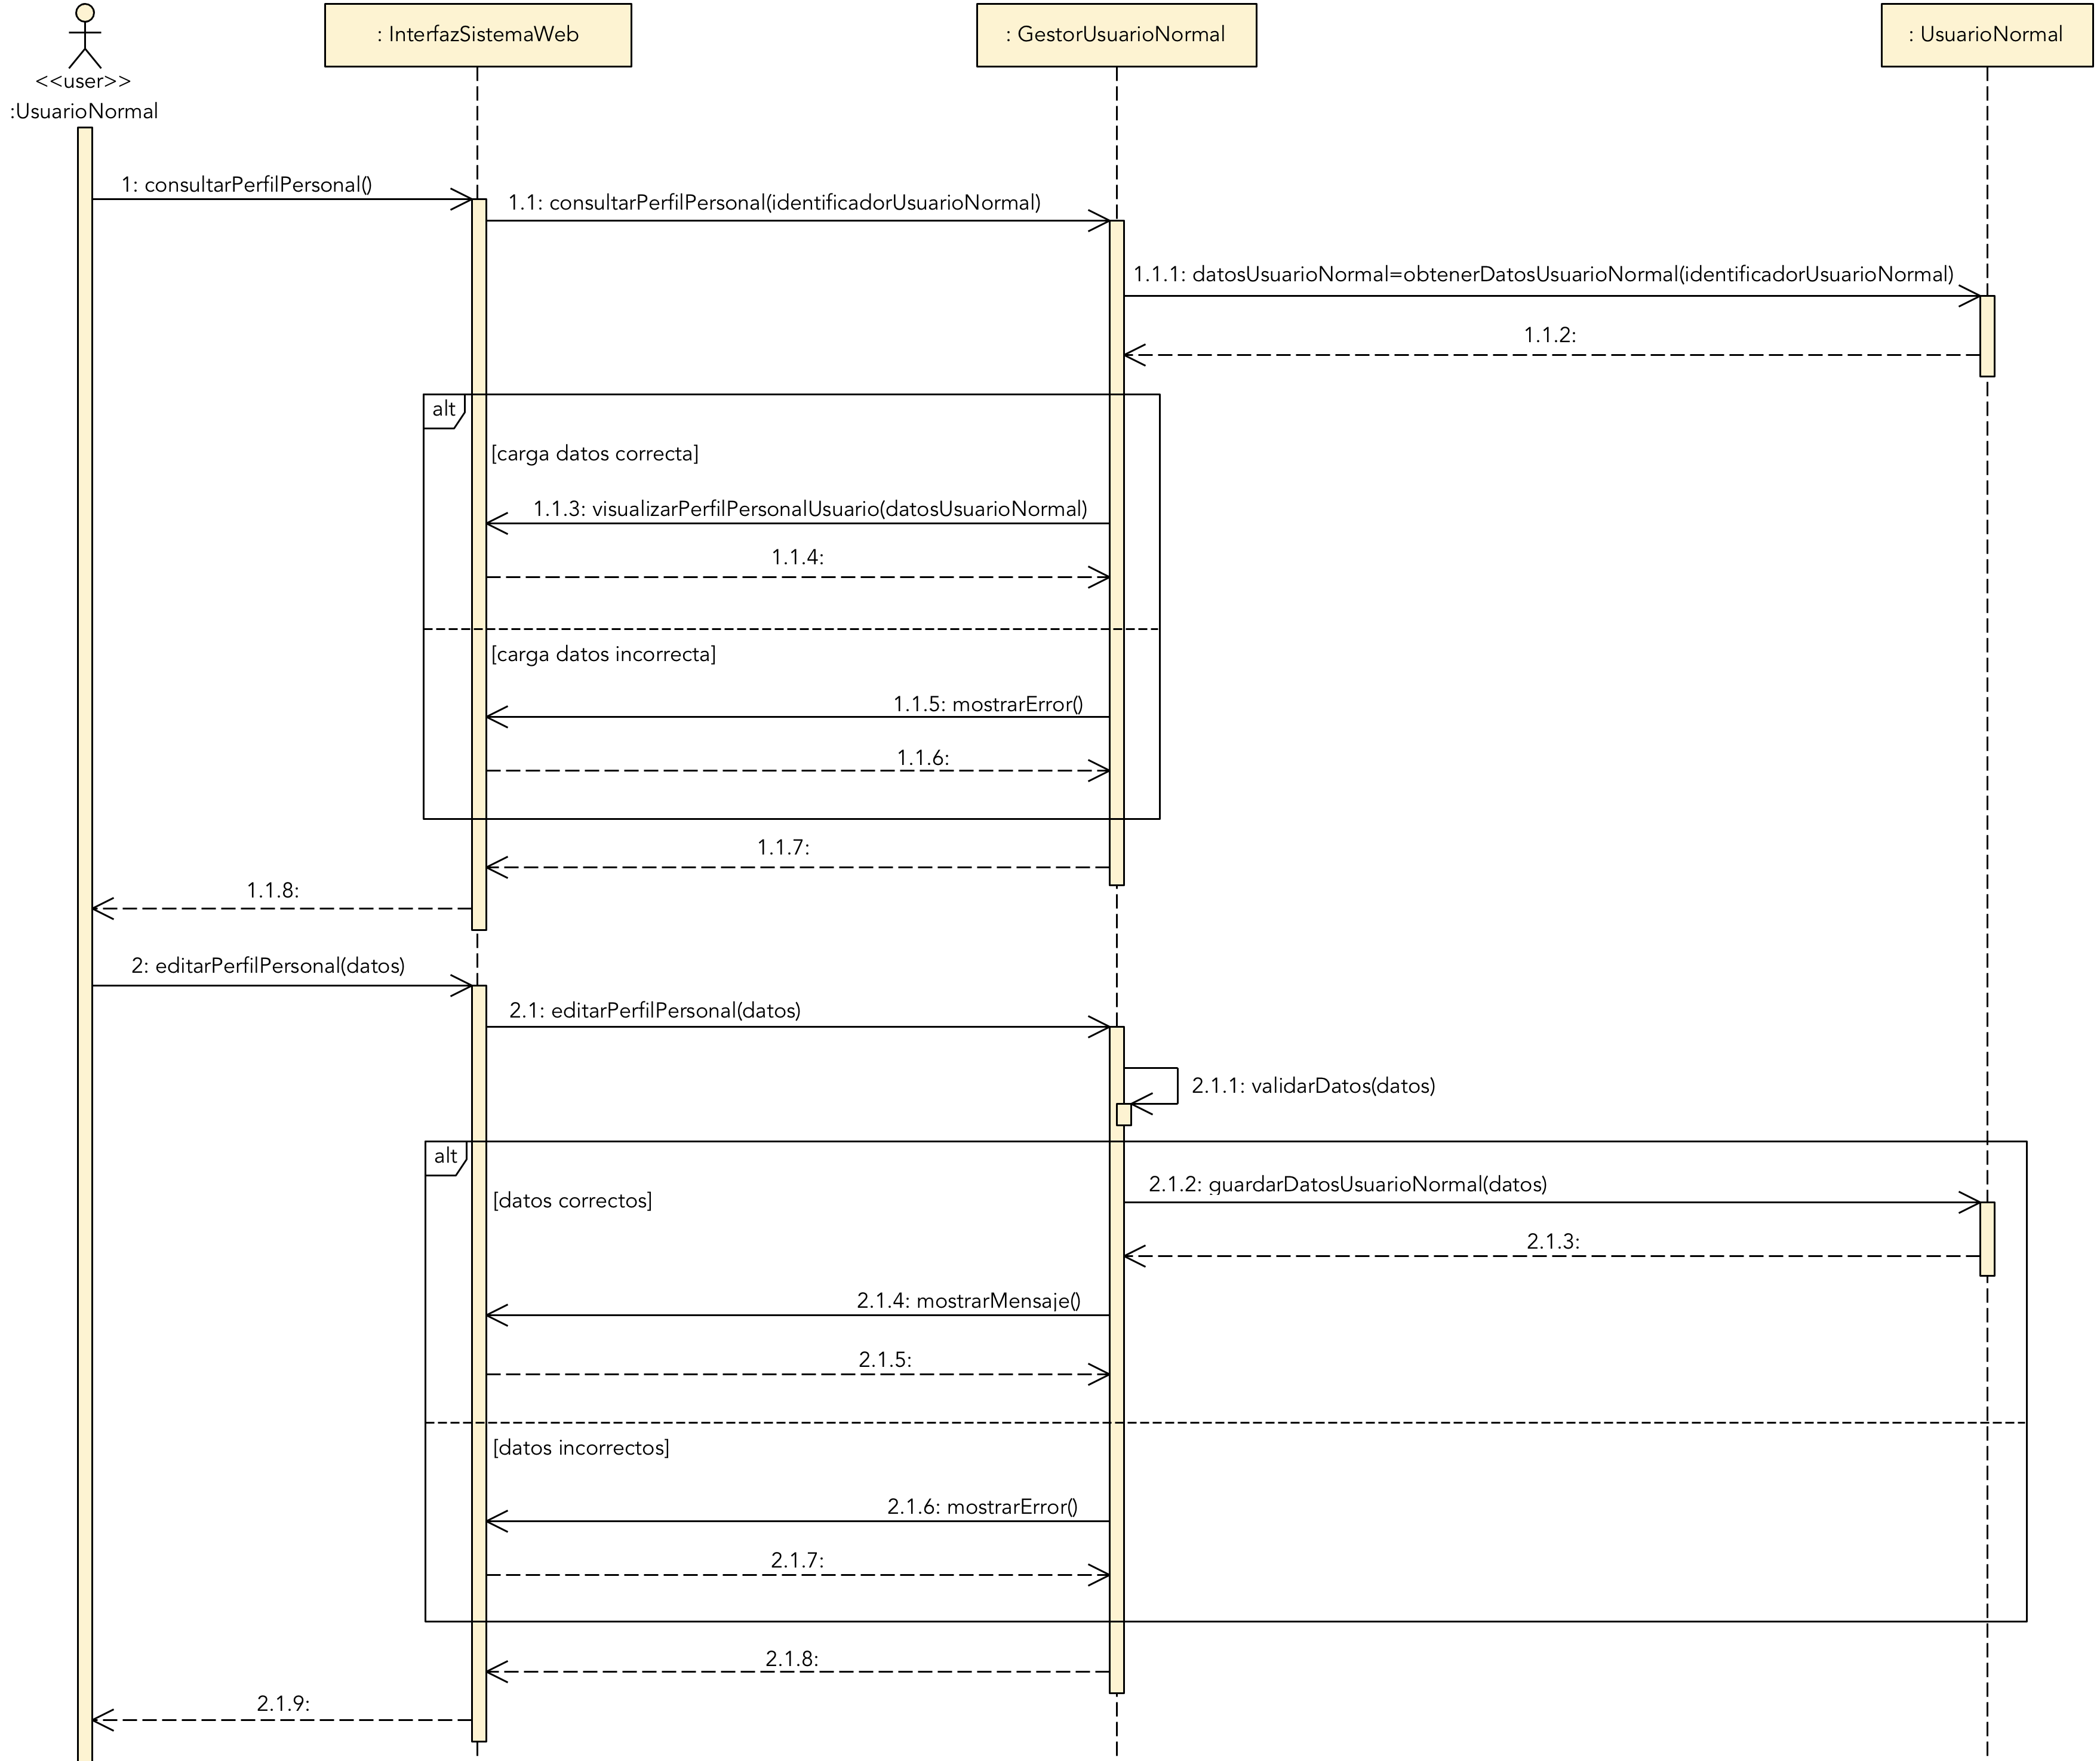
\includegraphics[width=17cm,height=20cm]{Images/analysis/secuencia/secuencia_perfilPersonal} \\
				\label{fig:ds_perfil} 
			\end{center}  
		\end{figure} 
		
		% NEW PAGE 
		\newpage
		
		\item Diagrama de secuencia de análisis: Consumir información sobre la trazabilidad del entorno (Figura \ref{fig:ds_consumirInfo}).
		
		\begin{figure}[!ht]   
			\caption{Diagrama de secuencia de análisis: Consumir información sobre la trazabilidad del entorno.} 
			\begin{center} 
	 			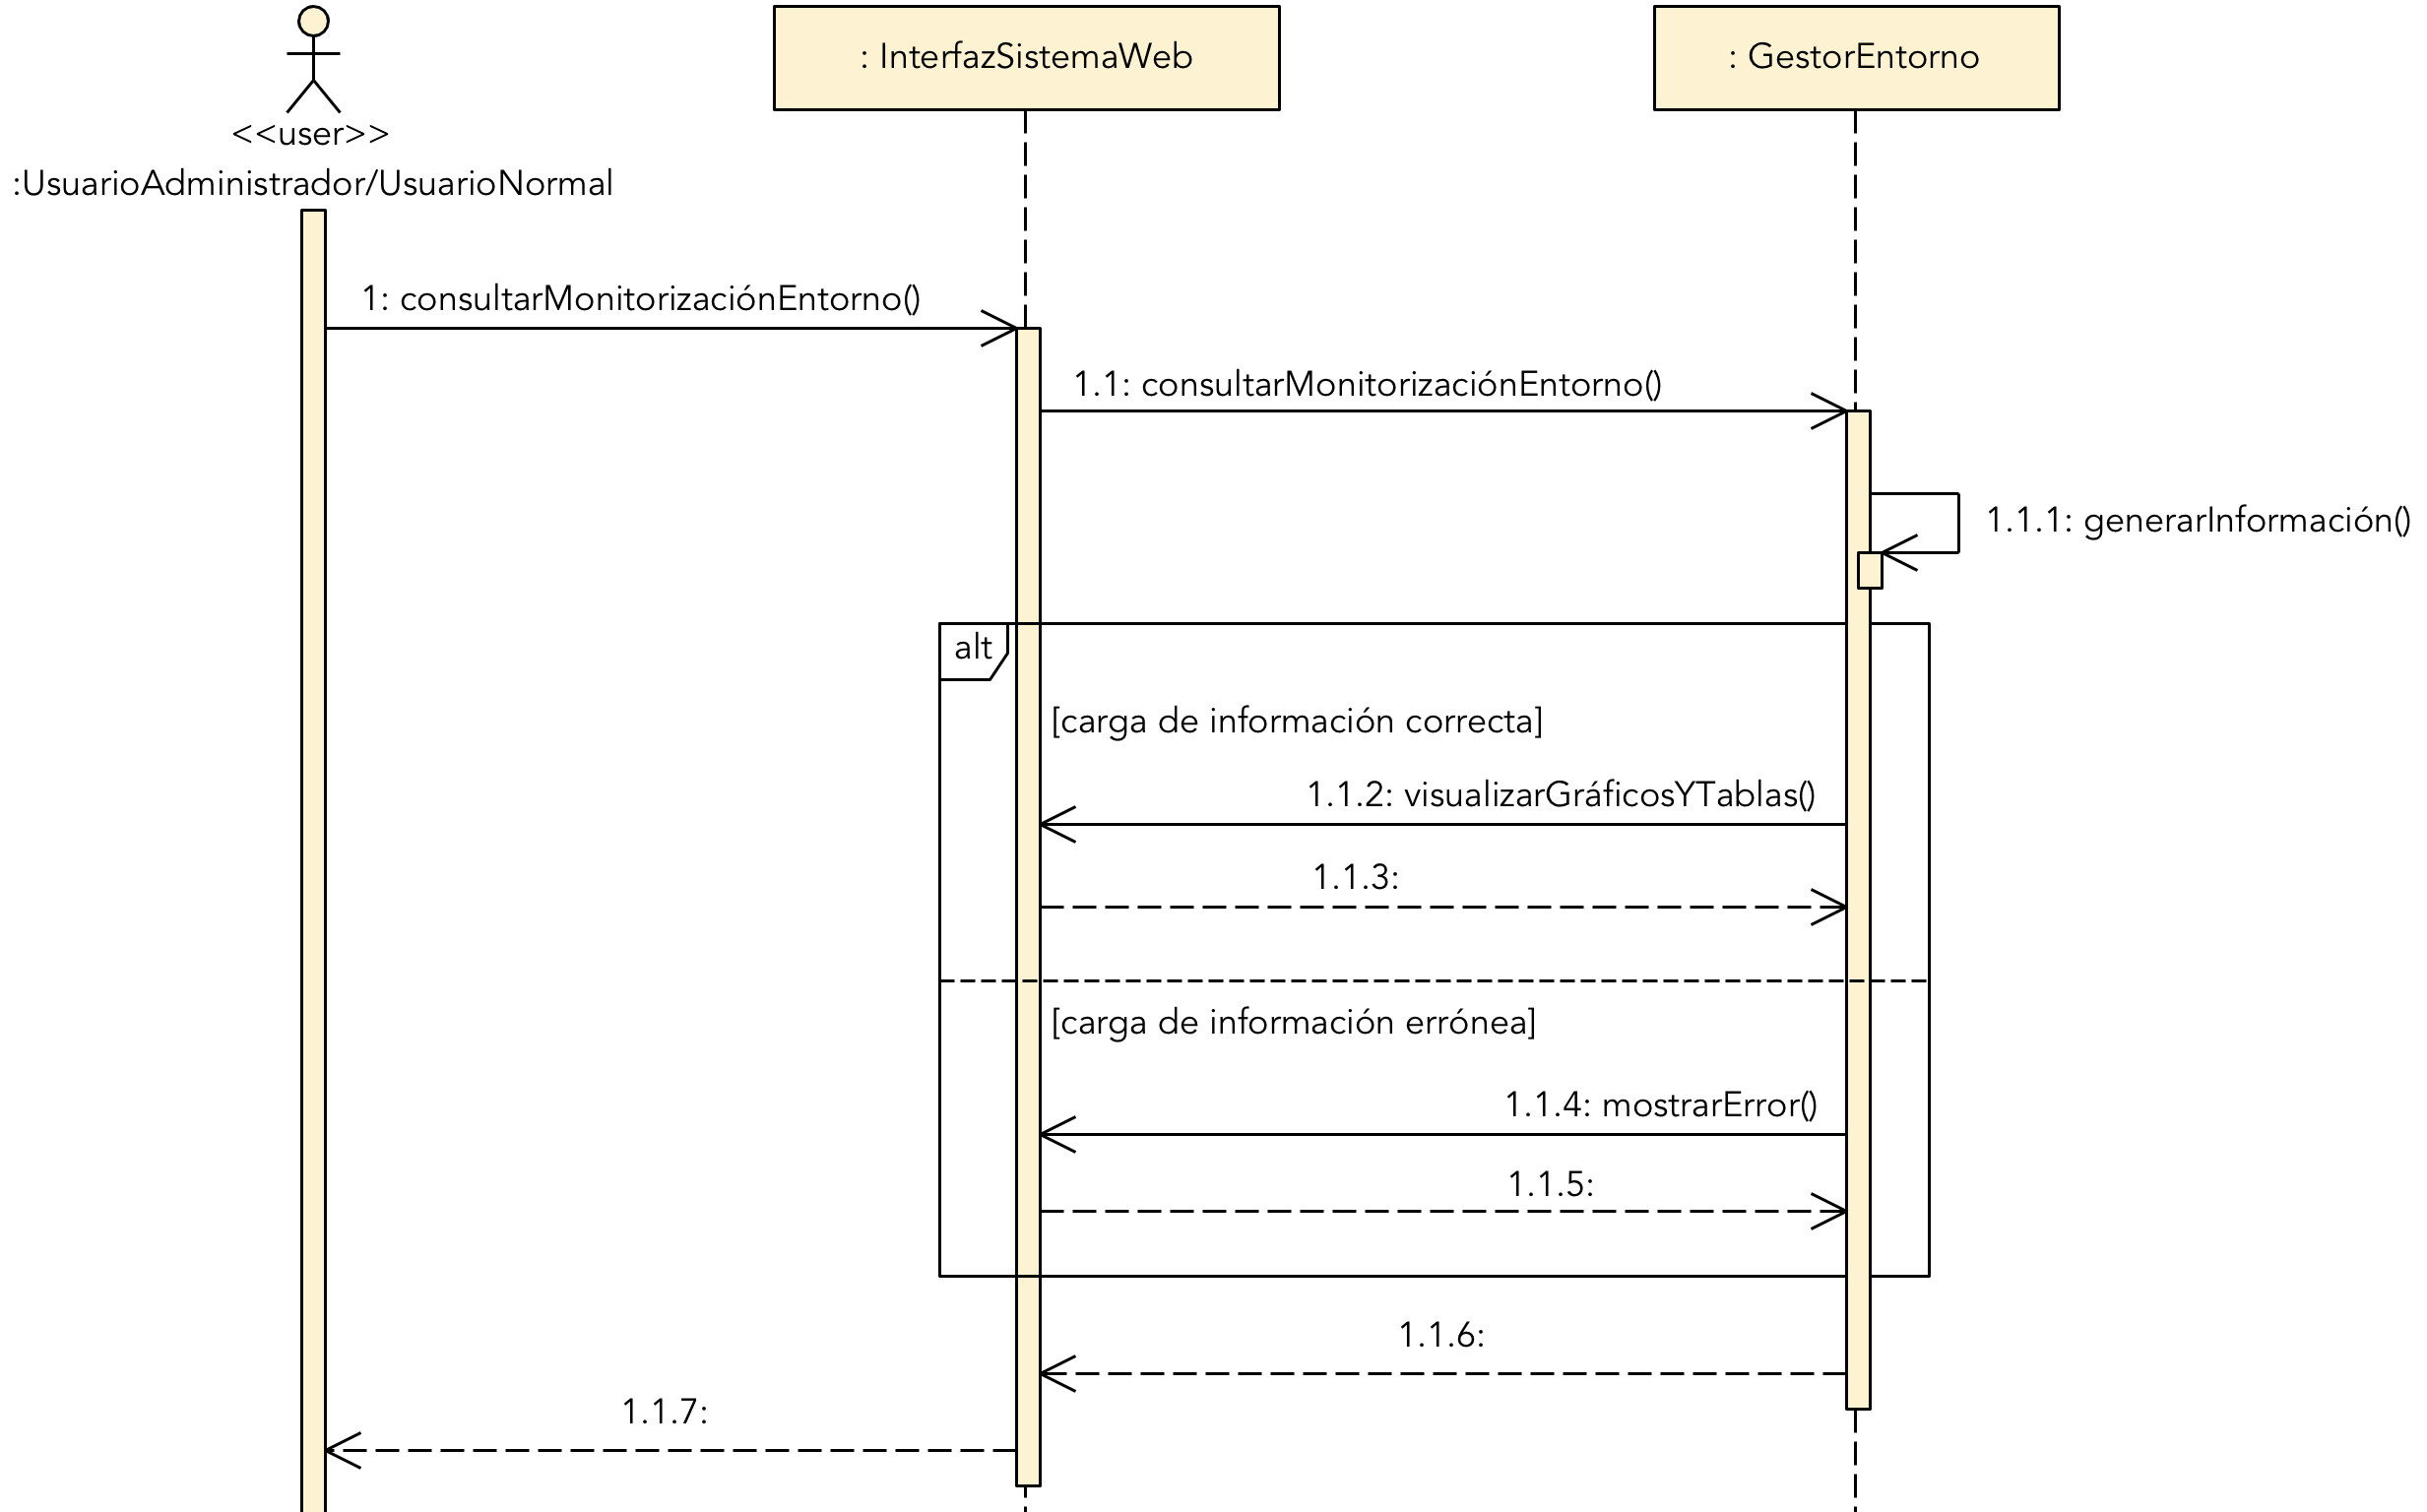
\includegraphics[width=17.5cm,height=13cm]{Images/analysis/secuencia/secuencia_consumirInformacion} \\
				\label{fig:ds_consumirInfo} 
			\end{center}  
		\end{figure} 
		
	\end{itemize}

	% Design
	\chapter{Diseño} \label{designChapter}
	
	\textbf{Resumen:} \textit{Dotar de un diseño y arquitectura al sistema tras haber recabado información durante la etapa de análisis, es esencial para formular y caracterizar la solución propuesta a implementar con el fin de que se ajuste a los requisitos fijados. En este capítulo, se aborda el diseño de la solución sugerida a través de diferentes diagramas.}
	
	% Section
	\section{Modelado de la arquitectura física del sistema}
	
	En esta sección se realiza una descripción de la arquitectura \textit{software} que guiará la implementación del proyecto de trazabilidad en entornos \gls{iot-a} (\textit{\gls{iot}}) mediante \gls{hyperledger}, llamado \textbf{Hyot}. La finalidad es detallar con mayor énfasis cómo esta solución se encuentra construida, qué componentes incluye y cómo son las relaciones entre ellos. Para ello, se explican los patrones utilizados y se muestran diferentes diagramas, elaborados con el lenguaje \gls{uml-a} (\textit{\gls{uml}}) \cite{uml}, que permiten modelar el sistema tanto a nivel físico como lógico.
		
	% Subsection
	\subsection{Descripción de la arquitectura}\label{architectureDescription}
	
	% TODO - Indicar también el sistema web en caso de que se ha utilizado ahí.

	El diseño de la arquitectura del sistema tiene como objetivo dotar a la solución de diferentes patrones arquitectónicos que resuelven problemas bien conocidos durante el desarrollo de sistemas \textit{software}, todo ello con el objetivo de favorecer la estructuración, mantenimiento y reutilización de la propia solución. En Hyot, se ha decidido implementar en la medida de lo posible el \gls{patrondiseño} arquitectónico de \textit{software} conocido como \gls{mvc} (\gls{mvc-a}) \cite{buschmann:mvc}, para todos los componentes que lo conforman, aplicando la variante pasiva la cual se caracteriza porque únicamente el controlador manipula el modelo. Dicho de otra forma, la vista no tiene ninguna responsabilidad sobre la lógica de dominio y únicamente se encarga de las tareas relacionadas con la interfaz de usuario (\textit{\gls{ui}} -\gls{ui-a}-). \\
	
	En el paradigma \gls{mvc-a}, las entradas del usuario o lógica de negocio, los modelos del mundo exterior y la retroalimentación visual son explícitamente separados y manejados por tres tipos de objetos distintos, cada uno especializado para un conjunto de tareas específicas:
	
	\begin{itemize}
		\item Modelo: contiene una representación específica de la información que maneja el sistema, su lógica de negocio, y sus mecanismos de persistencia. Lo ideal es que el modelo sea independiente del sistema de almacenamiento.
		\item Vista o \gls{ui-a}: conforma la información que se envía al usuario y los mecanismos de interacción.
		\item Controlador: actúa como intermediario entre el modelo y la vista y como modificador del primero, gestionando el flujo de información entre ellos y las transformaciones para adaptar los datos a lo solicitado por el usuario a través de la vista.
	\end{itemize}

	 Este patrón de implementación sencilla y ampliamente utilizado, que se basa en la idea de favorecer el mantenimiento y reutilización de código, y de la separación de conceptos y características, busca facilitar la tarea de desarrollo. Es por ello que se aplicó al proyecto Hyot. La Figura \ref{fig:design_mvc} muestra el esquema de este patrón en su variante pasiva, siendo el flujo de proceso habitual el especificado a continuación:
	
	\begin{enumerate}
		\item El usuario interactúa, de alguna forma, con la interfaz del sistema (interfaz web, terminal...).
		\item El controlador recibe la entrada del usuario y la gestiona, frecuentemente con un manejador de eventos.
		\item El controlador accede y notifica al modelo la acción del usuario lo que puede implicar un cambio de estado de éste.
		\item El controlador notifica a la vista de que el modelo ha sido modificado y delega a los objetos de ésta la tarea de actualizar la información de la interfaz.
		\item La interfaz del sistema espera nuevas interacciones del usuario, comenzando el ciclo de nuevo. 
	\end{enumerate}
	
	\begin{figure}[!ht]   
		\caption{Esquema del patrón arquitectónico \gls{mvc-a} pasivo.} 
		\begin{center} 
			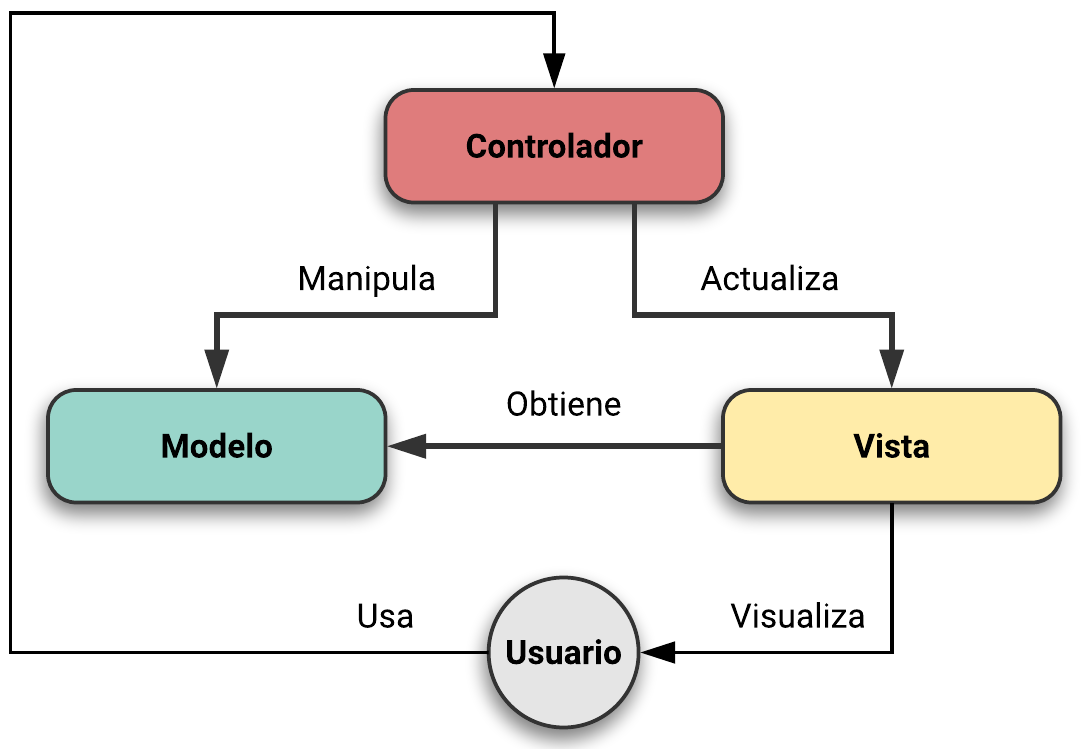
\includegraphics[width=8.5cm,height=4cm]{Images/design/mvc.png} \\
			\label{fig:design_mvc} 
		\end{center}  
	\end{figure}
	
	% TODO - Sistema web. Si se emplea pues mencionarlo aquí
	A parte de este patrón, también se ha implementado el patrón Singleton \cite{gof95}. Este patrón es un \gls{patrondiseño} creacional ampliamente conocido y utilizado en el desarrollo \textit{software} que está diseñado para garantizar la existencia de una única instancia de un objeto en toda la aplicación proporcionando así un punto único de acceso global. En sí, no se encarga de la creación de objetos sino de aplicar esta restricción durante la creación lo que proporciona los siguientes beneficios: acceso estricto a la instancia única, espacio de nombres reducido al no reservar nombres para variables globales, mayor número de variables de instancia, mayor flexibilidad. Su funcionamiento es sencillo y se reduce a (Figura \ref{fig:design_singleton}):
	
	\begin{enumerate}
		\item Privatizar el constructor de la clase Singleton, para que los usuarios no puedan crear instancias.
		\item Declarar en la clase Singleton una variable miembro privada que contenga la referencia a la instancia única que se quiere gestionar.
		\item Proveer en la clase Singleton una función o propiedad que brinde acceso a la única instancia gestionada. Los usuarios acceden a la instancia a través de esta función o propiedad.
	\end{enumerate}
	
	\begin{figure}[h]		
		\caption{Diagrama de clases y de secuencia del \gls{patrondiseño} creacional Singleton.}
 		\begin{subfigure}{0.5\textwidth}
 			\hbox{
 				\hspace{1cm}
 				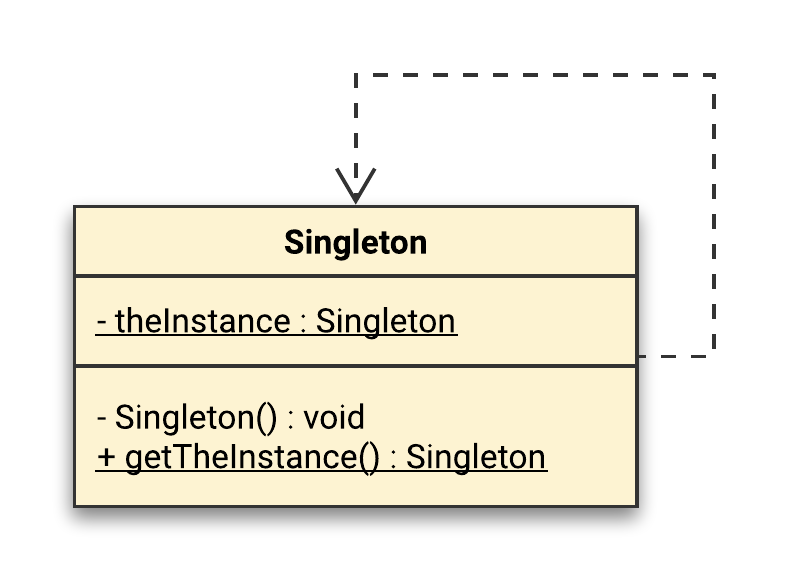
\includegraphics[width=5.5cm, height=5cm]{Images/design/singleton_uml.png} 
 			}
		\end{subfigure}
		\begin{subfigure}{0.5\textwidth}
			\hbox{
 				\hspace{2cm}
				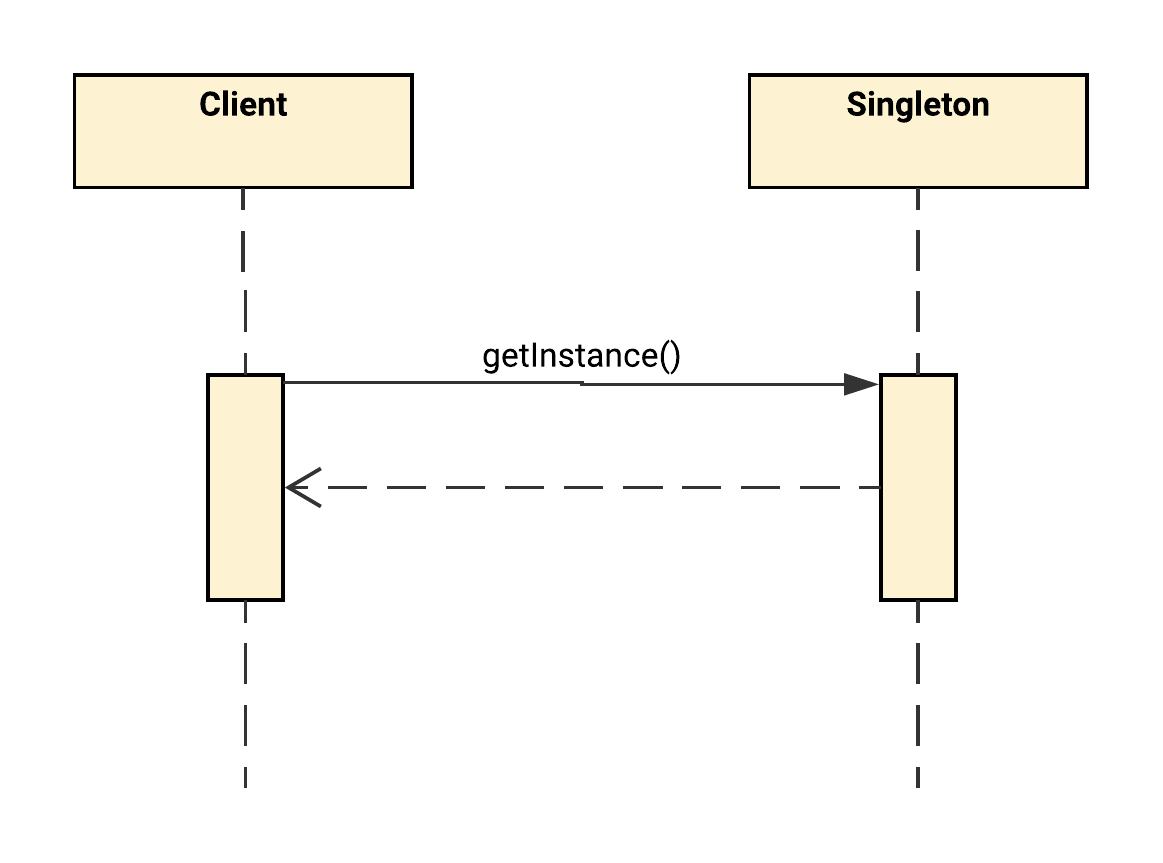
\includegraphics[width=6cm, height=7cm]{Images/design/singleton_secuencia}
			}
		\end{subfigure}
		\label{fig:design_singleton}
	\end{figure}
 	
	Este patrón ha sido empleado en el componente de monitorización de sucesos del entorno, en concreto en:

	\begin{itemize}
		\item El \textit{logger} para controlar el número de instancias que se generan de esta clase.
		\item En las importaciones de módulos. Por naturaleza, todos los módulos en \gls{python} se comportan como un patrón Singleton ya que se comprueba si el módulo ya ha sido importado. En caso afirmativo, lo retorna. En caso contrario, busca el módulo, lo inicializa y lo retorna por lo que únicamente se inicializa una vez definiendo un nombre o nombres en el espacio de nombres local.
	\end{itemize}
		
	% Subsection
	\subsection{Diagrama de capas}
	
	El diagrama de capas permite describir la arquitectura de la solución a alto nivel segmentando los elementos en grupos abstractos desde el punto de vista lógico, denominados capas -nodos en el diagrama-. Cada una puede describir las tareas principales que realizan los componentes del sistema, limitando el flujo de comunicación solamente a capas contiguas. El objetivo primordial de este modelo es el desacoplamiento de las diferentes partes que componen la solución \textit{software}, de forma que por ejemplo la creación de un nuevo componente visual o su modificación se pueda simplificar de gran manera al no requerir modificación alguna en el resto de capas, salvo la afectada lo que implicaría una reducción del acoplamiento entre componentes. \\
		
	La división en Hyot se ha realizado en 3 capas (Figura \ref{fig:design_layers}), cada una de ellas con una misión y favoreciendo así un diseño modular y escalable. A continuación, se describe cada capa identificada:
	
	\begin{itemize}
		\item Capa de presentación o de usuario: capa que presenta el sistema al usuario comunicándole la información y permitiéndole interactuar con el propio sistema a través de la captura de la información introducida por el usuario. Esta capa se comunica únicamente con la capa de negocio y se corresponde con el componente vista en el patrón \gls{mvc-a}. Debido a que se trata del nivel que expone y visualiza la información al usuario, debe implementar una \gls{ui-a} simple, fácil de usar, que presente claridad, coherencia en los textos y elementos, etc. En Hyot, esta capa estaría representada por el terminal donde se ejecutan los componentes \textit{\gls{script}} y la interfaz del sistema web.
	
		\item Capa de negocio o aplicativa: capa que contiene la lógica de negocio de la solución la cual está compuesta por una serie de reglas que se aplican sobre las peticiones del usuario para originar las respuestas que serán retornadas tras este proceso. Esta capa se comunica con la capa de presentación para recibir solicitudes y presentar los resultados y con la capa de datos para solicitar a los mecanismos de persistencia almacenar, modificar o recuperar información. En el paradigma \gls{mvc-a}, esta capa se corresponde con el componente controlador y haciendo referencia a la solución Hyot, la lógica de negocio comprendería toda aquella codificación, incluyendo módulos, clases, servicios, procesador de transacciones (\textit{\gls{transaction}}), etc., que trata la información introducida por el usuario, ya sea a través del terminal o la interfaz del sistema web o incluso aquella información que es introducida al sistema de manera automática procedente de fuentes de información externa como son los \glspl{sensor}, y genera respuestas.
		
		\item Capa de datos o de persistencia: representa el modelo, es decir, el lugar donde reside la información. Esta capa es la responsable de la gestión y almacenamiento permanente de los datos según las peticiones recibidas de la capa de negocio, correspondiendo al modelo en el paradigma \gls{mvc-a}. En Hyot, estaría formada por los 3 diferentes mecanismos de persistencia implementados (explicados con más detalle en la sección \ref{persistencia}. \nameref{persistencia}).		 
	\end{itemize} 	
	
	\begin{figure}[!ht]   
		\caption{Hyot - Diagrama de capas.} 
		\begin{center} 
			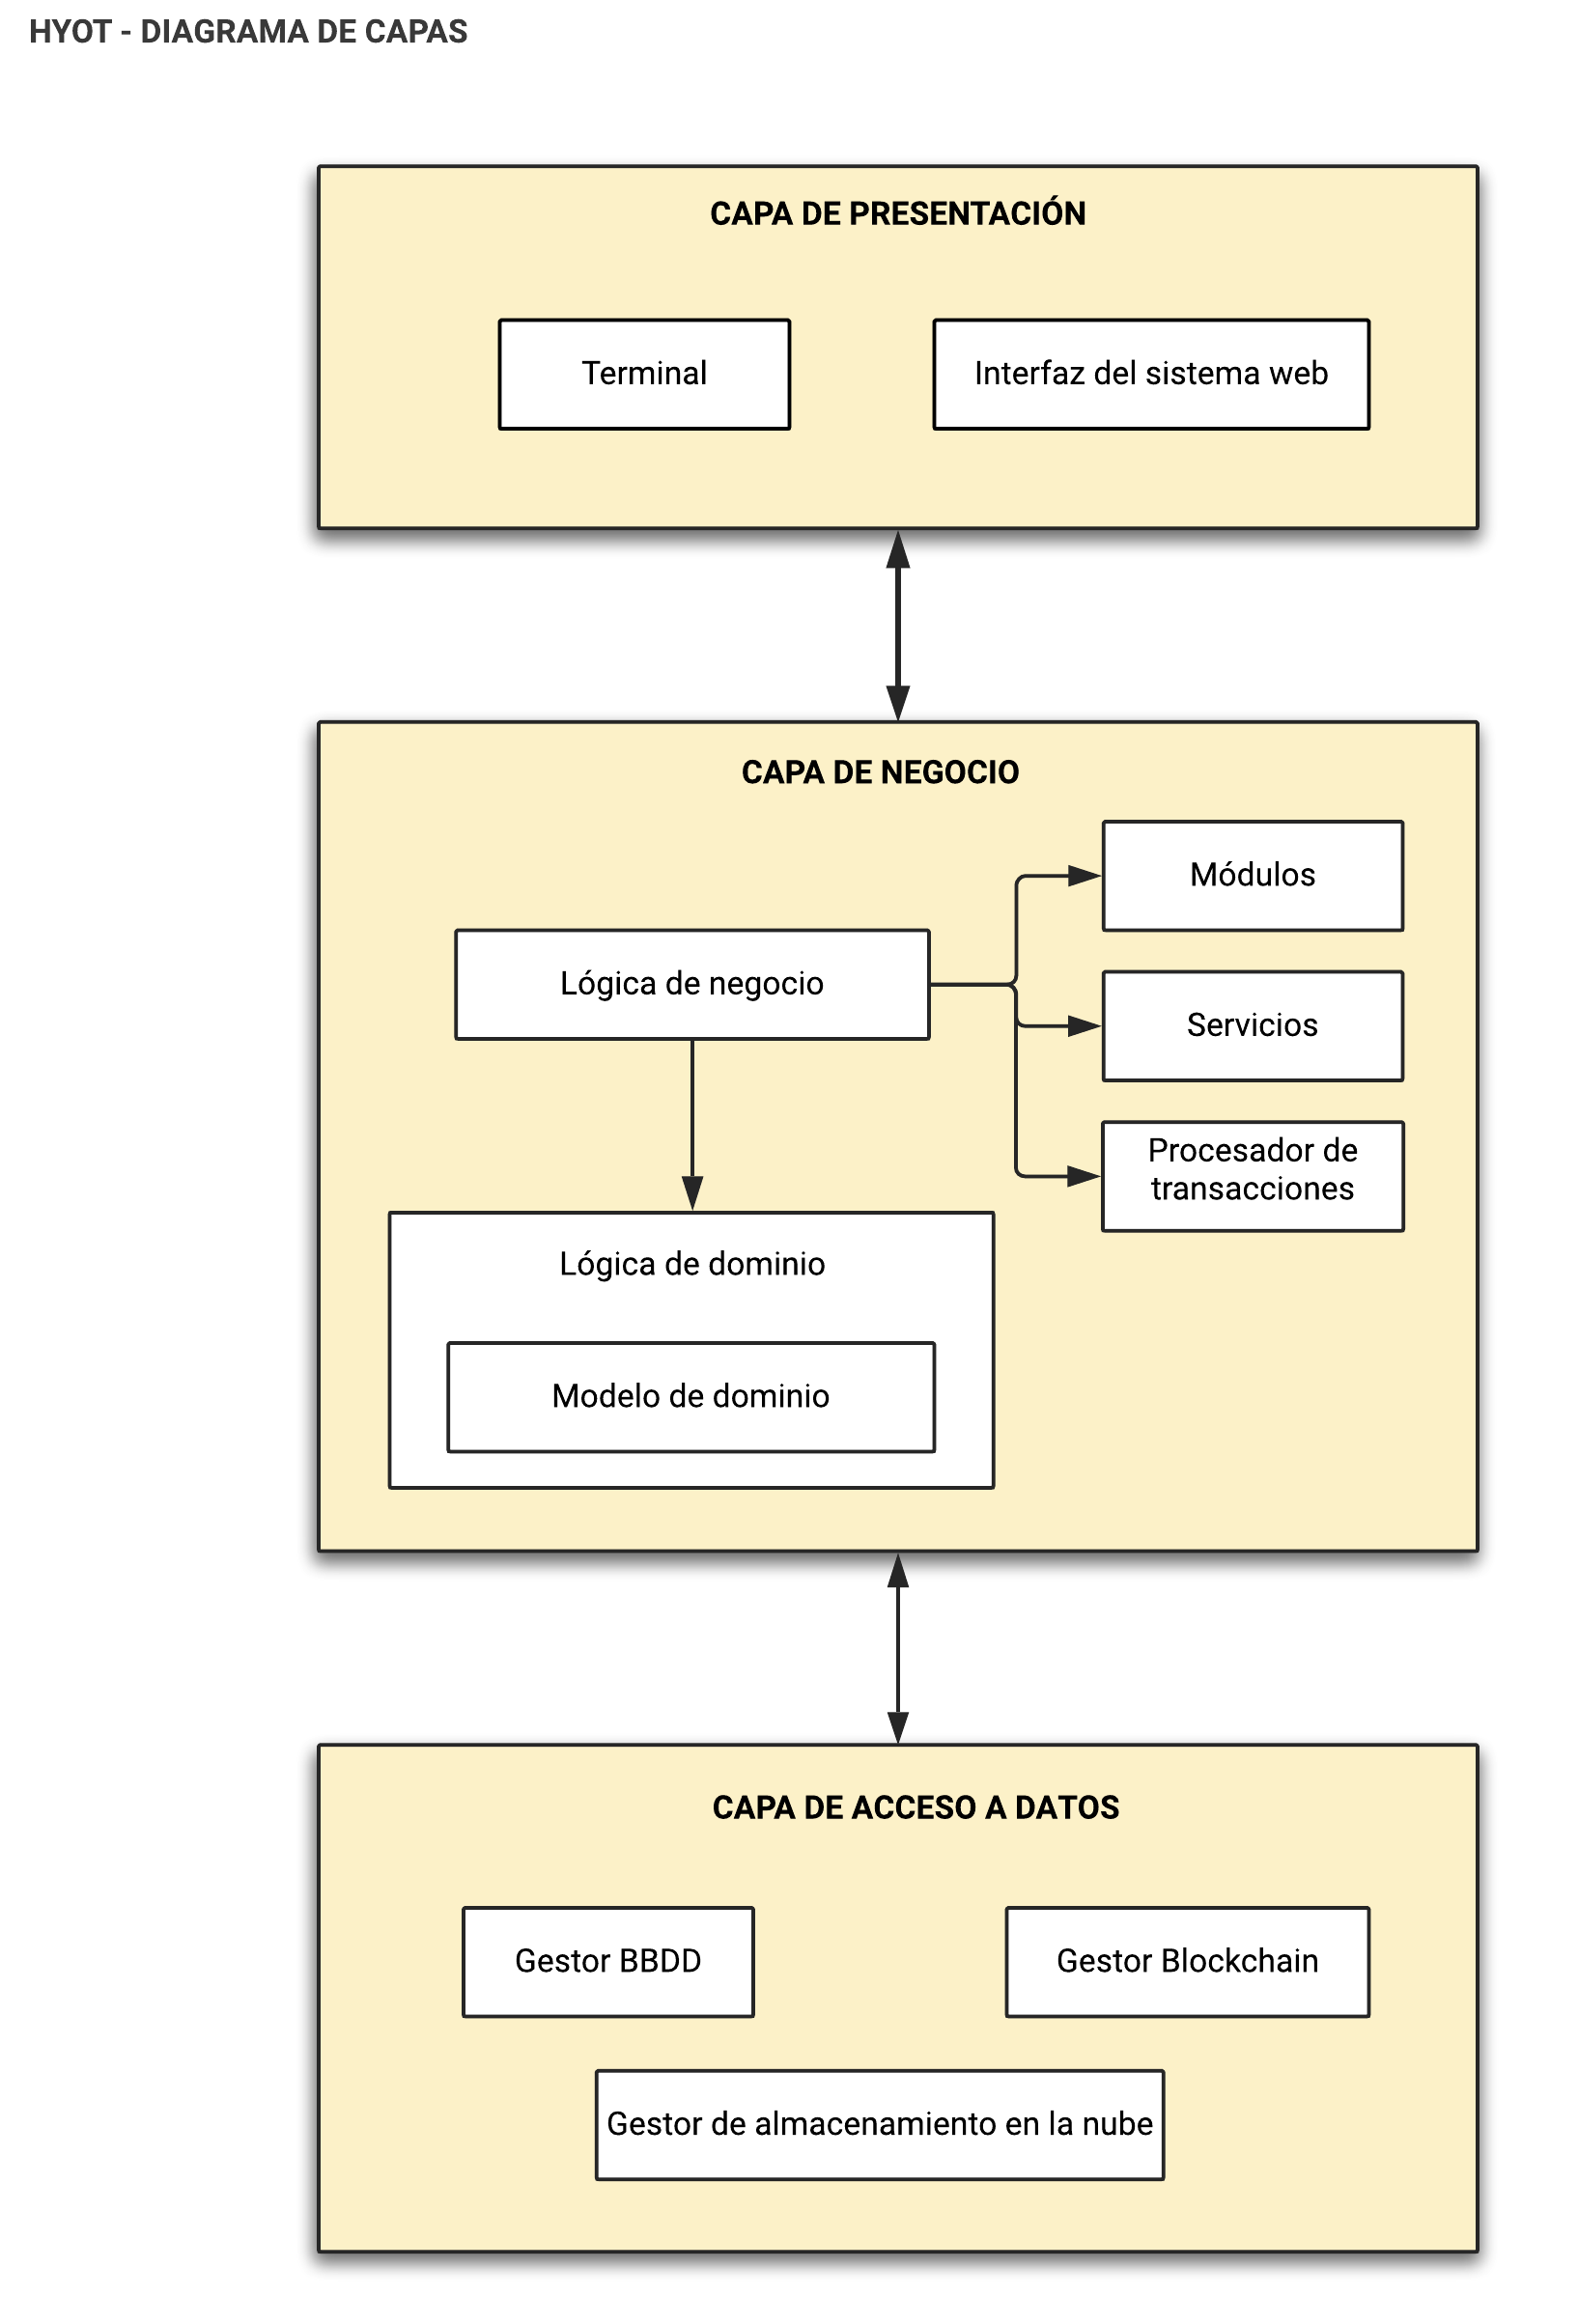
\includegraphics[width=12cm,height=15cm]{Images/design/d_layers} \\
			\label{fig:design_layers} 
		\end{center}  
	\end{figure}	
	
	% Subsection
	\subsection{Diagrama de despliegue} \label{d_deployment} % TODO - Adaptar con sistema web
	
	El diagrama de despliegue modela la arquitectura en tiempo de ejecución de un sistema, es decir, muestra la topología del sistema, la estructura de los componentes \textit{hardware}, los componentes \textit{software} que se ejecutan en cada nodo y la forma en la que las distintas partes están conectadas entre sí. \\
 		
	En Hyot, se ha optado por implementar una arquitectura centralizada basada en el \gls{clienteservidor} y en el modelo \textit{3-tier} (3 niveles) lo que significa que las capas lógicas se encuentran distribuidas de forma física en 3 componentes distintos. Este modelo es una extensión del modelo tradicional en 2 niveles que pretende aumentar el desacomplamiento entre servidor/es y clientes a través de la introducción de un nivel intermedio para separar el servidor en dos componentes: servidor que contiene la lógica de negocio y servidores que contienen los mecanismos de persistencia. Además, este modelo presenta mayor flexibilidad y modularidad, escalabilidad, extensibilidad, seguridad, reusabilidad de componentes, aislamiento frente a cambios en otras capas e independencia frente a cambios en los componentes de persistencia. \\
	
	El motivo de esta elección se debe a que se trata de la arquitectura que mejor concuerda con el sistema debido a la existencia de un conjunto de clientes que demandan un servicio proporcionado por el conjunto de servidores de la solución. Además, la transferencia de información entre éstos se puede optimizar al recudir la carga de trabajo y el número de peticiones de cada uno de ellos y de utilizar protocolos de comunicación de bajo nivel muy rápidos reduciendo el tráfico de red. Cabe indicar que esta arquitectura favorecerá el rendimiento en situaciones de saturación donde la carga solicitada será mayor que en el contexto y entorno actual de prueba. Desglosando la arquitectura mostrada en el diagrama de despliegue (Figura \ref{fig:design_deployment}), se pueden observar los siguientes niveles:
	
	\begin{itemize}
		\item Primer nivel: en este primer nivel se ubica la capa lógica de presentación donde se diferencian dos tipos de dispositivos \textit{hardware}:
			\begin{itemize}
				\item Dispositivo que representa un cliente delgado ya que simplemente actúa como intermediario entre el usuario y el servidor web, no implementando ningún aspecto de la lógica de negocio. Este dispositivo puede ser cualquier ordenador o dispositivo móvil con conexión a Internet el cual permitirá a los usuarios interactuar con el sistema web mediante un navegador utilizando los protocolos \gls{http-a} (\textit{\gls{http}}) y \gls{https-a} (\textit{\gls{https}}).
				\item Dispositivo, \gls{raspberry} (\gls{raspberry-a}), que representa un cliente pesado o grueso ya que presenta carga de cómputo y capacidad de procesamiento de datos en el propio dispositivo, gracias a la ejecución de un componente del proyecto Hyot. Este dispositivo interactúa directamente mediante los protocolos \gls{http-a} y \gls{https-a} con los mecanismos de persistencia desplegados.
			\end{itemize}
				 		
		\item Segundo nivel: en este nivel se localiza el servidor del sistema web desplegado en la plataforma como servicio (\textit{\gls{paas}} -\gls{paas-a}-) \cite{gonzalez:2011:TCCS} \gls{cloudfoundry} de IBM Cloud. Este sistema web interactúa directamente mediante los protocolos \gls{http-a} y \gls{https-a} con los mecanismos de persistencia desplegados.
		
		\item Tercer nivel: en el último nivel se hallan los tres mecanismos de persistencia utilizados: el servicio de almacenamiento en la nube, el gestor de bases de datos desplegado en el servicio IBM Cloud y el servicio de \Gls{blockchain} (\gls{blockchain-a}) desplegado en una máquina virtual (\textit{\gls{vm}} -\gls{vm-a}-) en Microsoft Azure.
	\end{itemize}
	  
	\begin{figure}[!ht]   
		\caption{Hyot - Diagrama de despliegue.} 
		\begin{center} 
			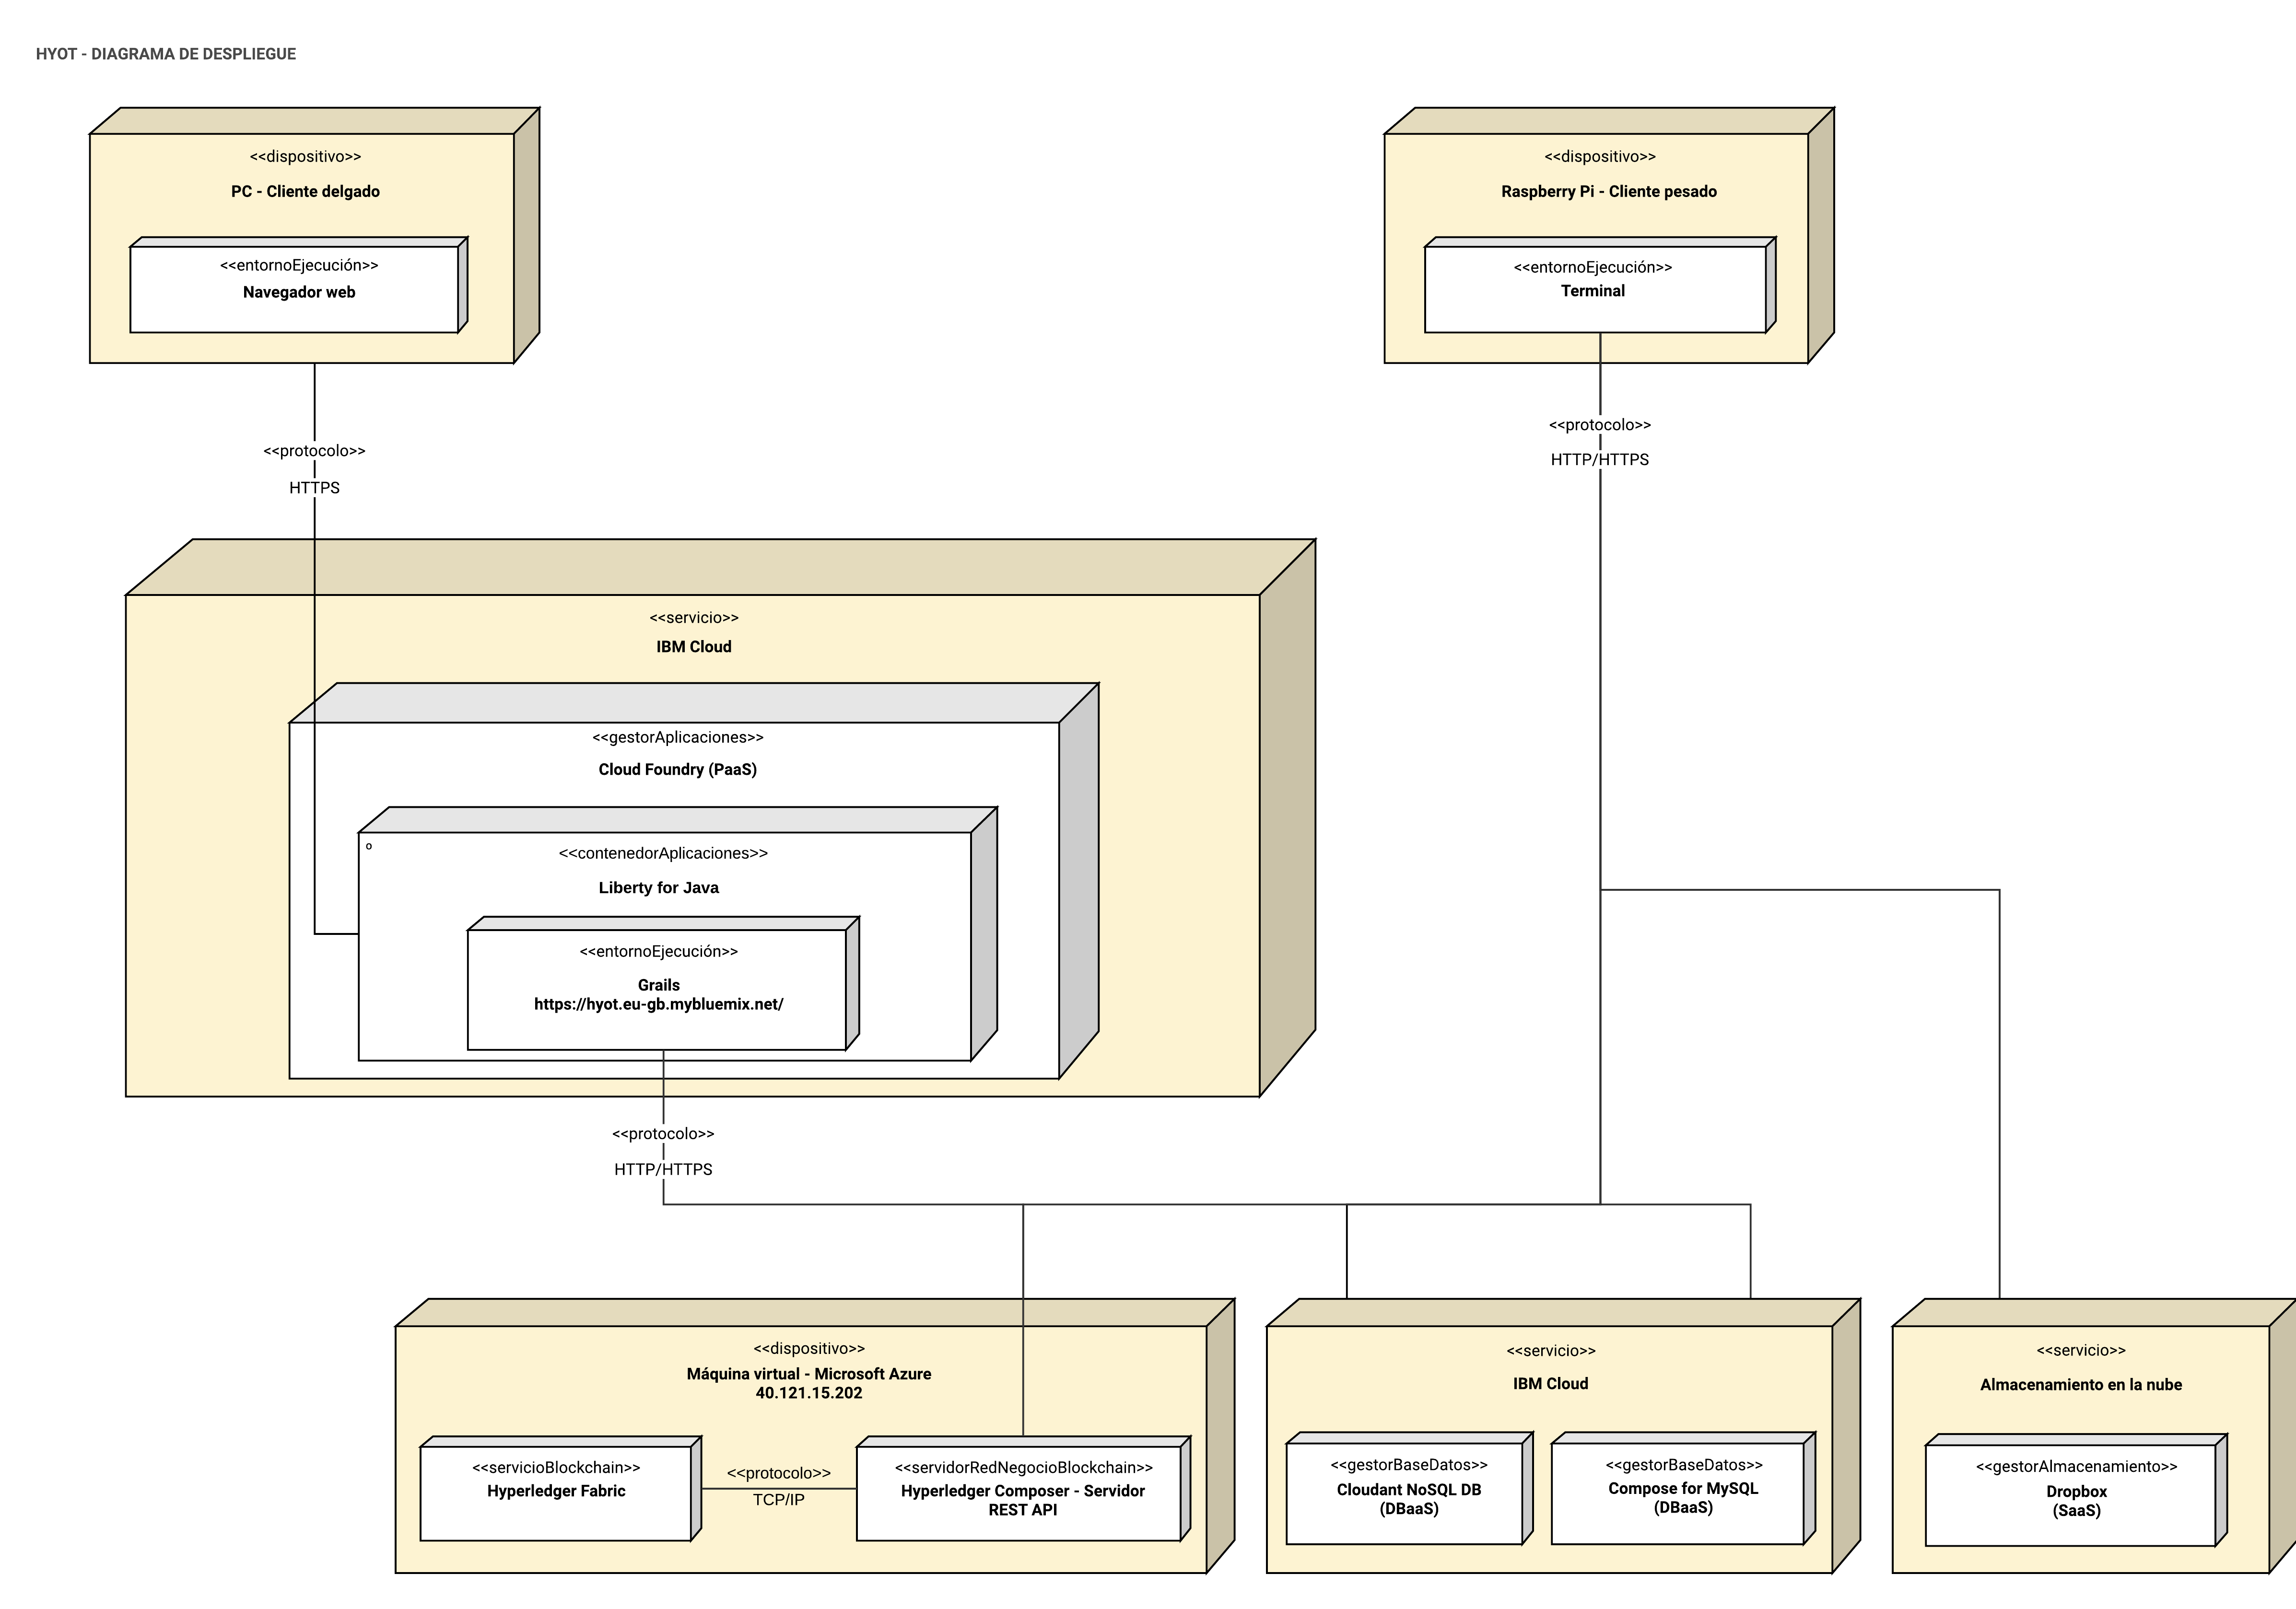
\includegraphics[width=17.5cm,height=17cm]{Images/design/d_deployment.png} \\
			\label{fig:design_deployment} 
		\end{center}  
	\end{figure}	

	% Subsection
	\subsection{Diagrama de paquetes} % TODO - Adaptar con sistema web
	
	El diagrama de paquetes muestra el sistema dividido en agrupaciones lógicas individuales exponiendo las dependencias existentes entre ellas y proporcionando una descomposición de la jerarquía lógica. Los paquetes, mecanismo de agrupación de elementos modelados con \gls{uml-a}, facilitan el manejo de los modelos en un sistema complejo definiendo un espacio de nombres y están normalmente organizados para maximizar la coherencia interna dentro de cada paquete y minimizar el acoplamiento externo entre los paquetes. La Figura \ref{fig:design_packages} muestra el diagrama de paquetes definido:
	
	\begin{figure}[!ht]   
		\caption{Hyot - Diagrama de paquetes.} 
		\begin{center} 
			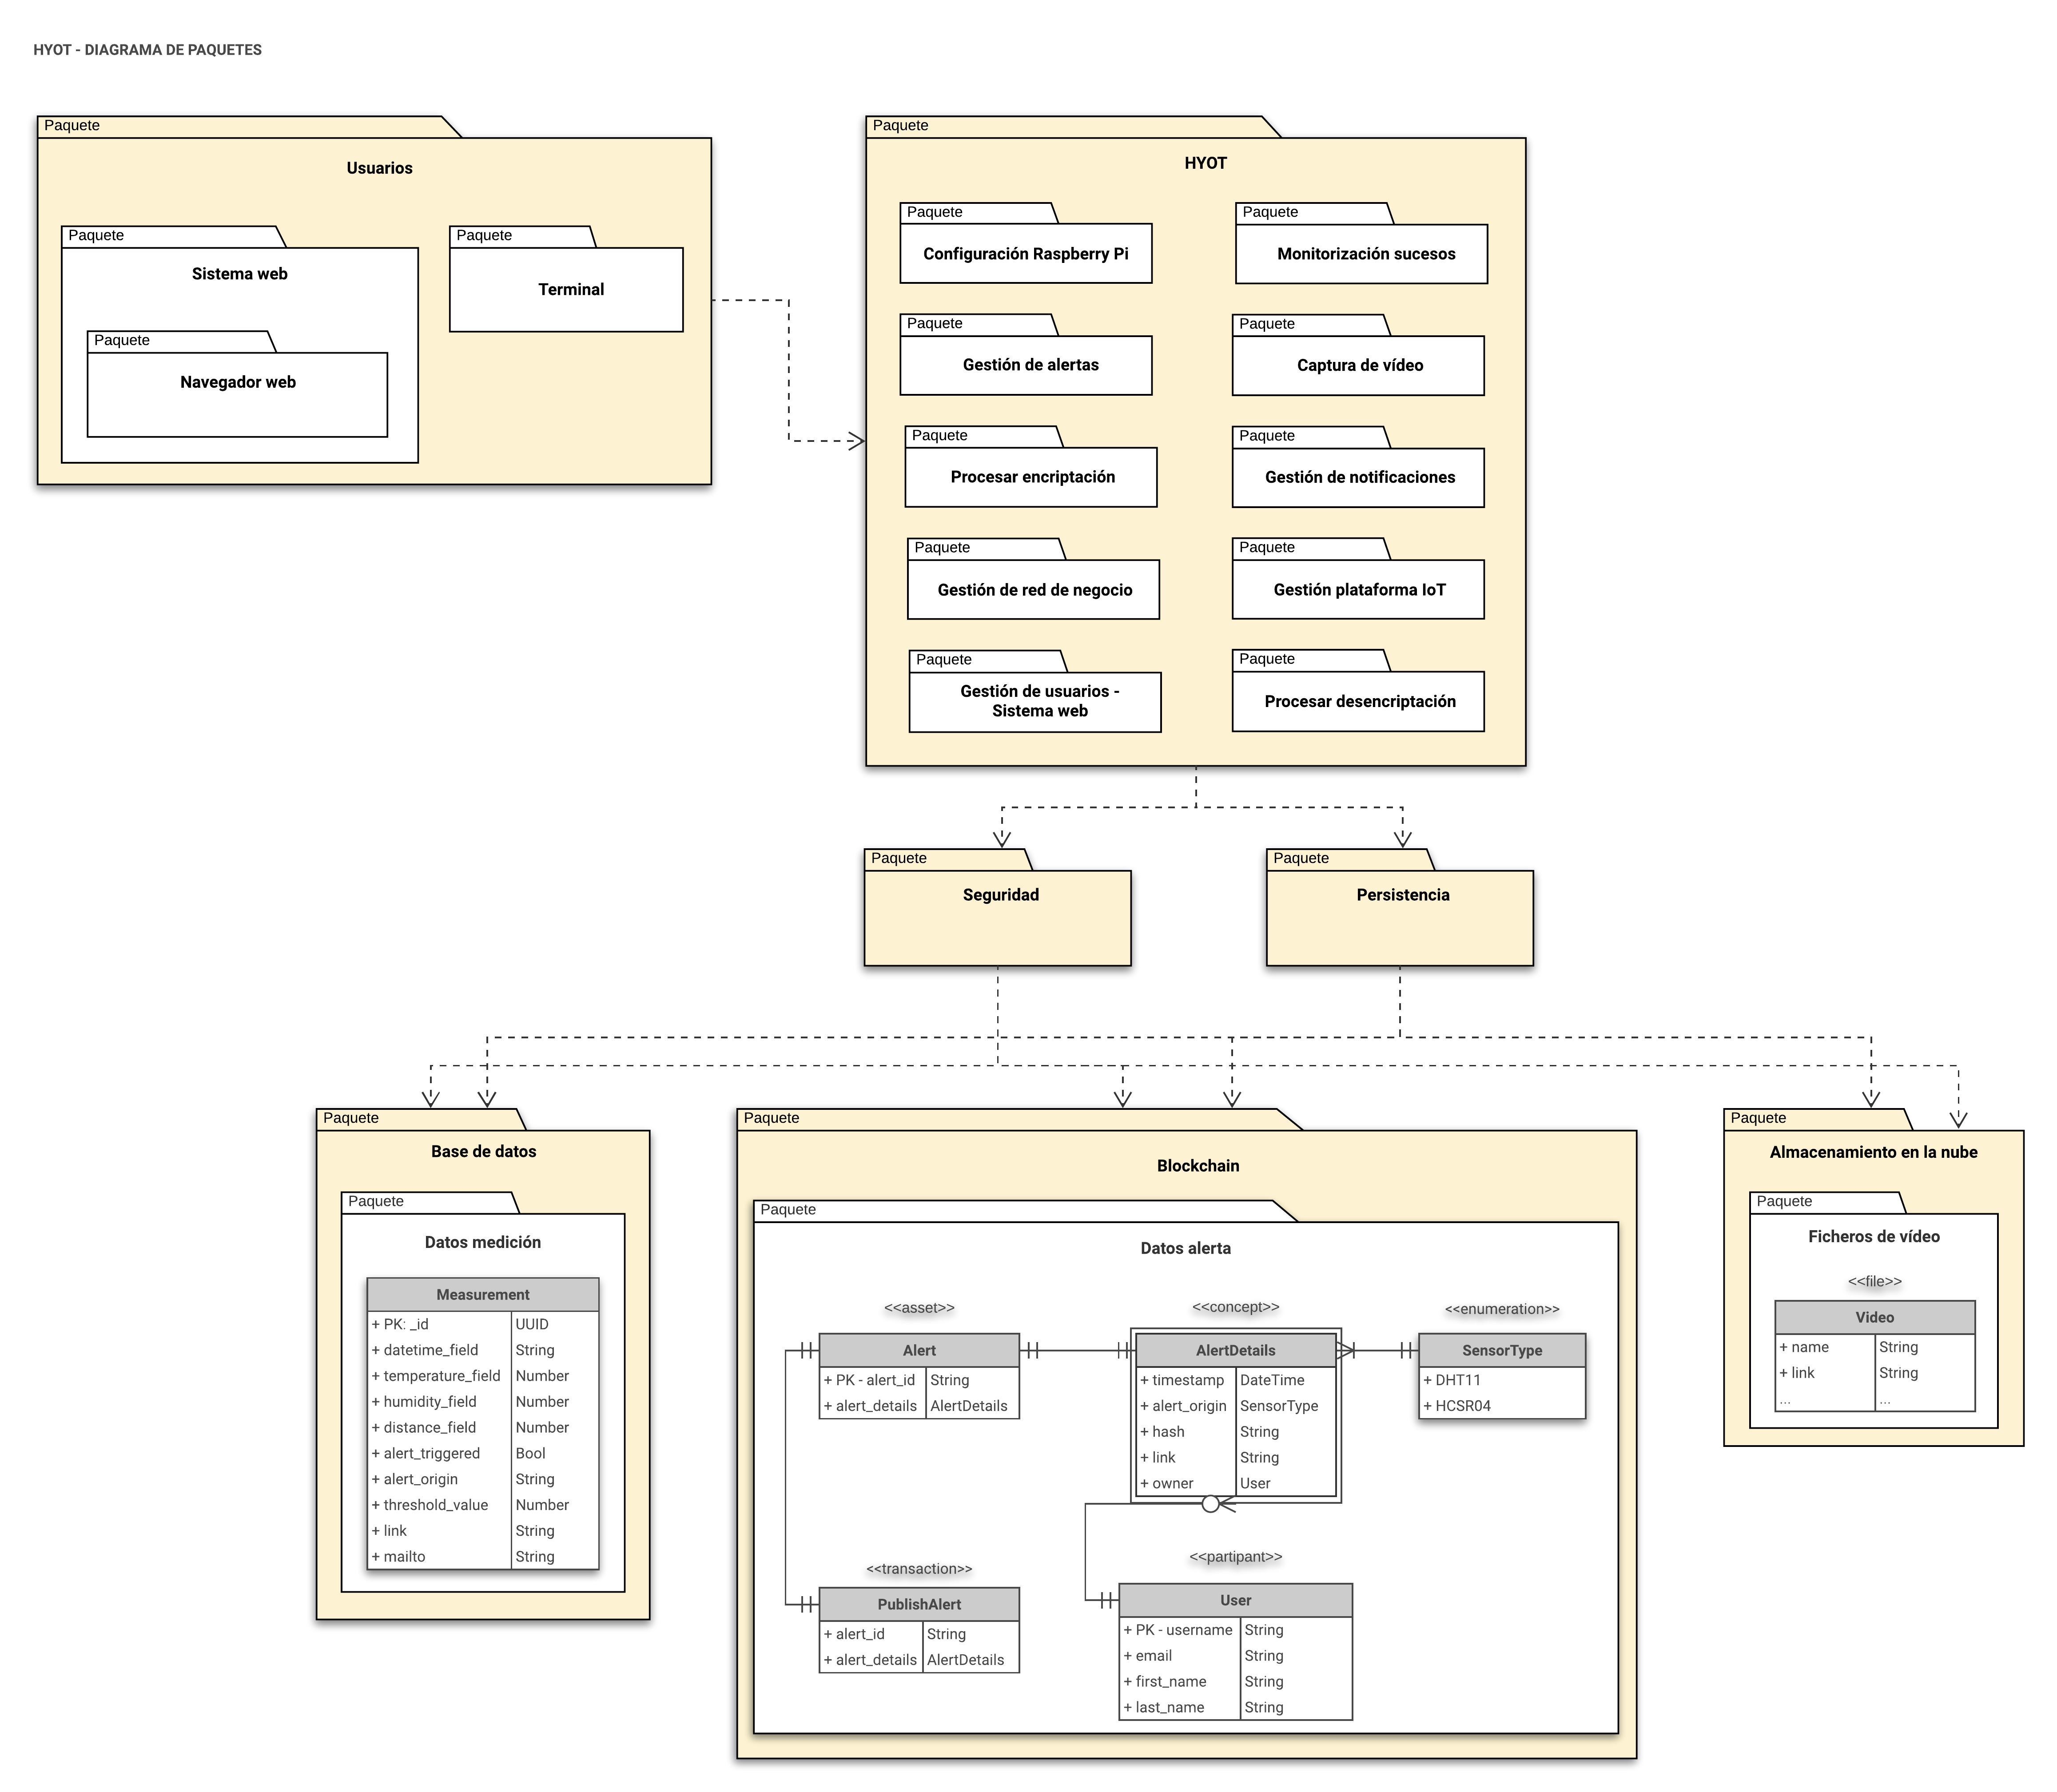
\includegraphics[width=18cm,height=18cm]{Images/design/d_packages} \\
			\label{fig:design_packages} 
		\end{center}  
	\end{figure}	
	
	% Subsection
	\subsection{Diagrama de vista lógica} % TODO - Adaptar con sistema web
		
	El diagrama de vista lógica es una abstracción a gran escala del modelado de paquetes, subsistemas y clases, buscando mostrar los requerimientos funcionales del sistema y cómo éste se debe comportar y funcionar. La Figura \ref{fig:design_logicview} muestra el diagrama definido: \\
	
	\begin{figure}[!ht]   
		\caption{Hyot - Diagrama de vista lógica.} 
		\begin{center} 
			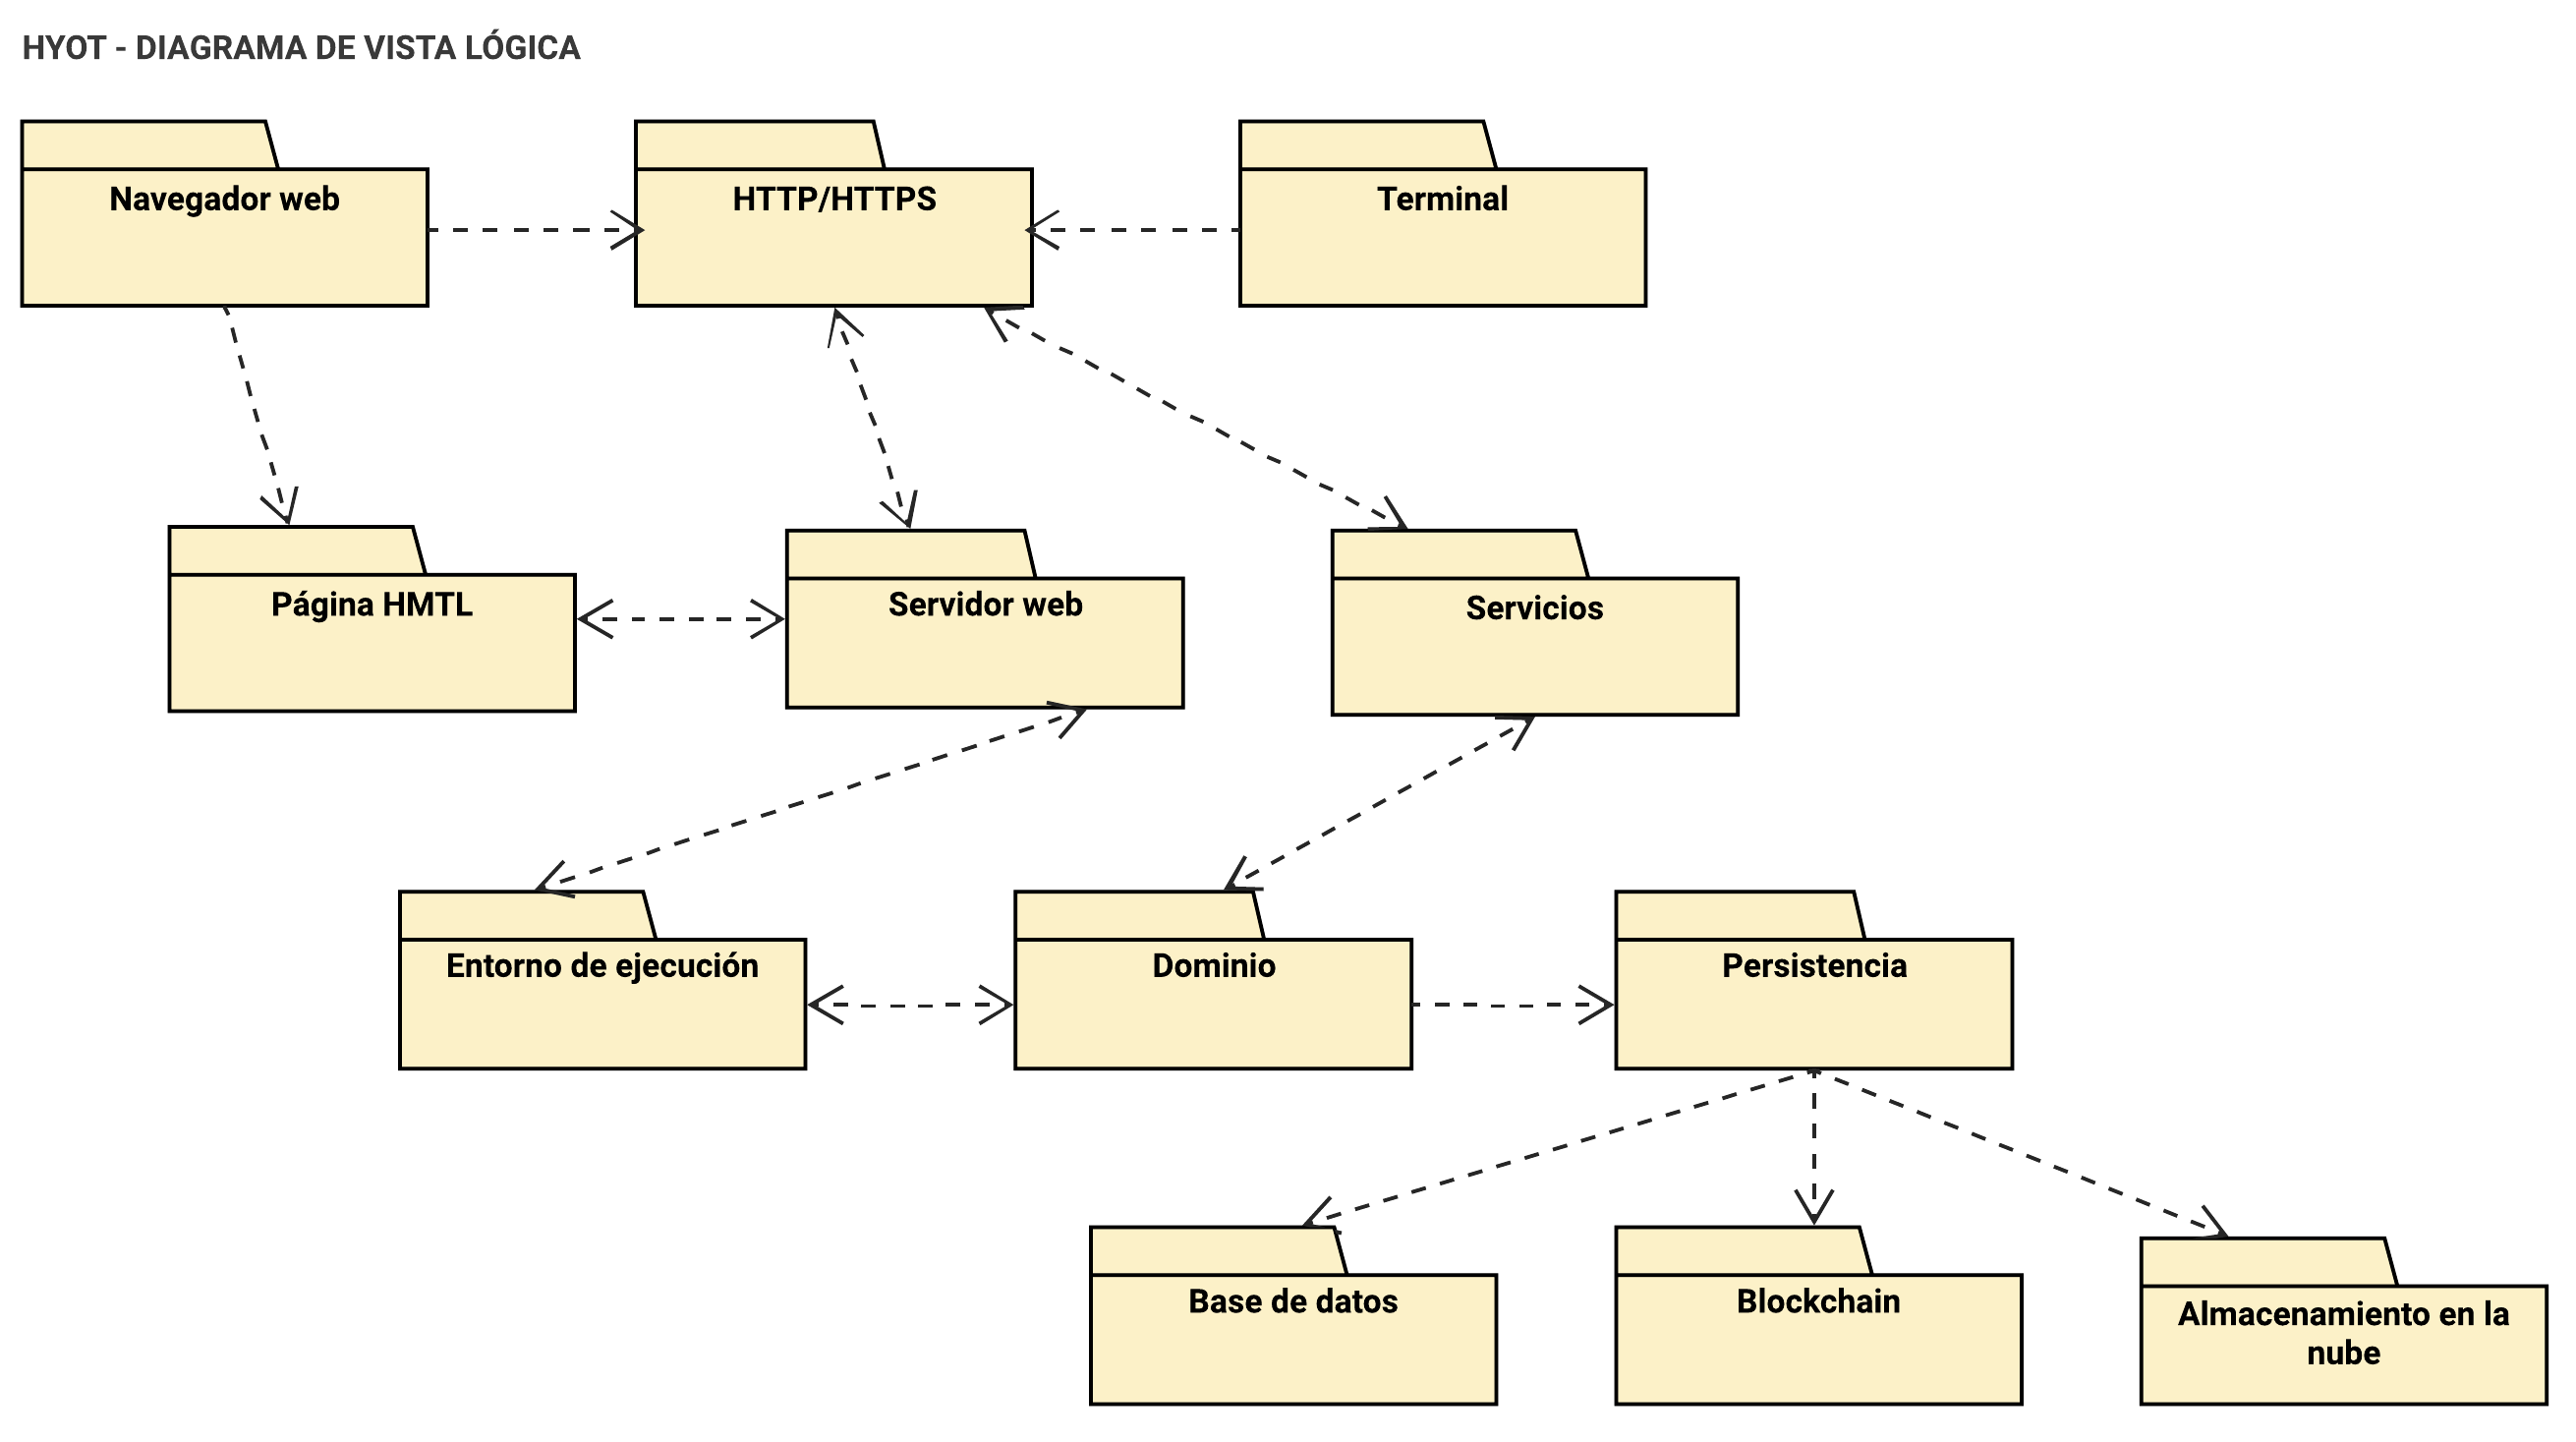
\includegraphics[width=18cm,height=14cm]{Images/design/d_logicview} \\
			\label{fig:design_logicview} 
		\end{center}  
	\end{figure}	
	
	% Subsection
	\subsection{Capa de persistencia} \label{persistencia} % TODO - Adaptar con sistema web
	
	La capa de persistencia es una capa independiente de la capa de negocio que está encargada de abstraer, encapsular y resolver completamente el acceso a datos de las aplicaciones cliente que la utilicen, siendo posible trabajar con varios mecanismos de persistencia ya sean gestores de bases de datos u otros medios o servicios que permitan almacenar información. Su objetivo es ser la única capa que conoce cómo son persistidos los objetos de dominio de la aplicación y cómo pueden ser recuperados abstrayendo el choque de impedancias entre objetos y tablas relacionales o no relacionales. Las capas superiores no interactúan directamente con el gestor de base de datos, sino que lo hacen mediante la interfaz expuesta por la capa de persistencia logrando así la independencia buscada. Esto proporciona la principal ventaja de las capas de abstracción, la portabilidad debido a que es posible cambiar la estrategia en la que los objetos son persistidos e incluso modificar la tecnología o el motor utilizado, sin impactar al código restante que se ubica en capas superiores. \\
	
	En el proyecto Hyot, se emplean tres mecanismos de persistencia para la información manejada, cada uno de ellos con una finalidad distinta:
	
	\begin{itemize}
		\item Base de datos (\gls{bbdd-a}): distribuida como servicio (\textit{\gls{dbaas}} -\gls{dbaas-a}-) \cite{gonzalez:2011:TCCS} en la nube de tipo no relacional (NoSQL) y orientada a documentos en formato \gls{json-a} (\textit{\gls{json}}) que almacena los valores de cada medición efectuada. La decisión de su elección se tomó en base a las necesidades de escalabilidad y versatilidad de la información almacenada puesto que la principal característica es que se encuentran optimizadas para grandes volúmenes de datos con un esquema flexible lo que se alinea con el contexto del proyecto: mediciones constantes y posibilidad de ampliación del proyecto a otros dispositivos \gls{iot-a} lo que ampliaría o modificaría el modelo de información a almacenar. Además, la elección de ser distribuida como un servicio y no usar una desplegada localmente se debe a facilitar el proceso de puesta en marcha y configuración y la disponibilidad total ya que se encuentra físicamente remota pero lógicamente en local.
		\item Servicio de almacenamiento: para almacenar los artefactos encriptados y firmados que son generados por el componente de monitorización de sucesos del entorno. Debido a su tamaño y tipología lo más adecuado es su almacenamiento en un servicio en la nube donde estén siempre disponibles.	
		\item \Gls{blockchain} (\gls{blockchain-a}): mecanismo de persistencia principal de Hyot donde se almacena aquella información que se quiera salvaguardar de cualquier posible alteración por una parte no autorizada y cuyo almacenaje en una \gls{bbdd-a} no proporciona la seguridad requerida.
	\end{itemize}
	
	% Subsubsection
	\subsubsection{Diagrama Entidad-Relación}
	
	El diagrama Entidad-Relación es un modelo de datos basado en una percepción del mundo real que consiste en un conjunto de objetos básicos llamados entidades y relaciones entre estos objetos para representar las entidades relevantes de un sistema así como sus interrelaciones y propiedades. Se puede obtener con la técnica, ingeniería inversa la cual permite obtener información y el diseño a partir de un sistema y así poder comprender y determinar el esquema lógico y conceptual de la \gls{bbdd-a}. \\
	
	La Figura \ref{fig:design_er} muestra el diagrama para el proyecto Hyot, donde se diferencian cada uno de los mecanismos de persistencia definidos\footnote{En el caso  del servicio de almacenamiento, al ser un servicio externo no se pueden controlar los atributos que almacena ya que únicamente se envía el fichero. Sin embargo, para hacer entendible el modelo y la información usada en el proyecto se especifican dos atributos y su estereotipo de fichero.} junto con las entidades que lo conforman. Además, cada entidad puede poseer un estereotipo\footnote{Las entidades que conforman el mecanismo de persistencia \gls{blockchain-a} se explicará con más detalle en la sección \ref{businessNetwork}. \nameref{businessNetwork} ya que sus estereotipos coinciden con los elementos del modelo de la red de negocio.}, unos atributos y tipo junto con la especificación en caso de existir del atributo que actuará como clave primaria o PK para identificar un registro único en el mecanismo de persistencia. Como particularidad del diagrama, indicar que la entidad \texttt{AlertDetails} es una entidad débil lo que quiere decir que su existencia depende de otra entidad (\texttt{Alert}) y no posee atributos únicos o clave primarias. Su estereotipo \texttt{<<concept>>} -proveniente de la tecnología \gls{hyperledgercomposer} (\gls{hyperledgercomposer-a})- viene a significar esto mismo.
	
	\begin{figure}[!ht]   
		\caption{Hyot - Diagrama Entidad-Relación.} 
		\begin{center} 
			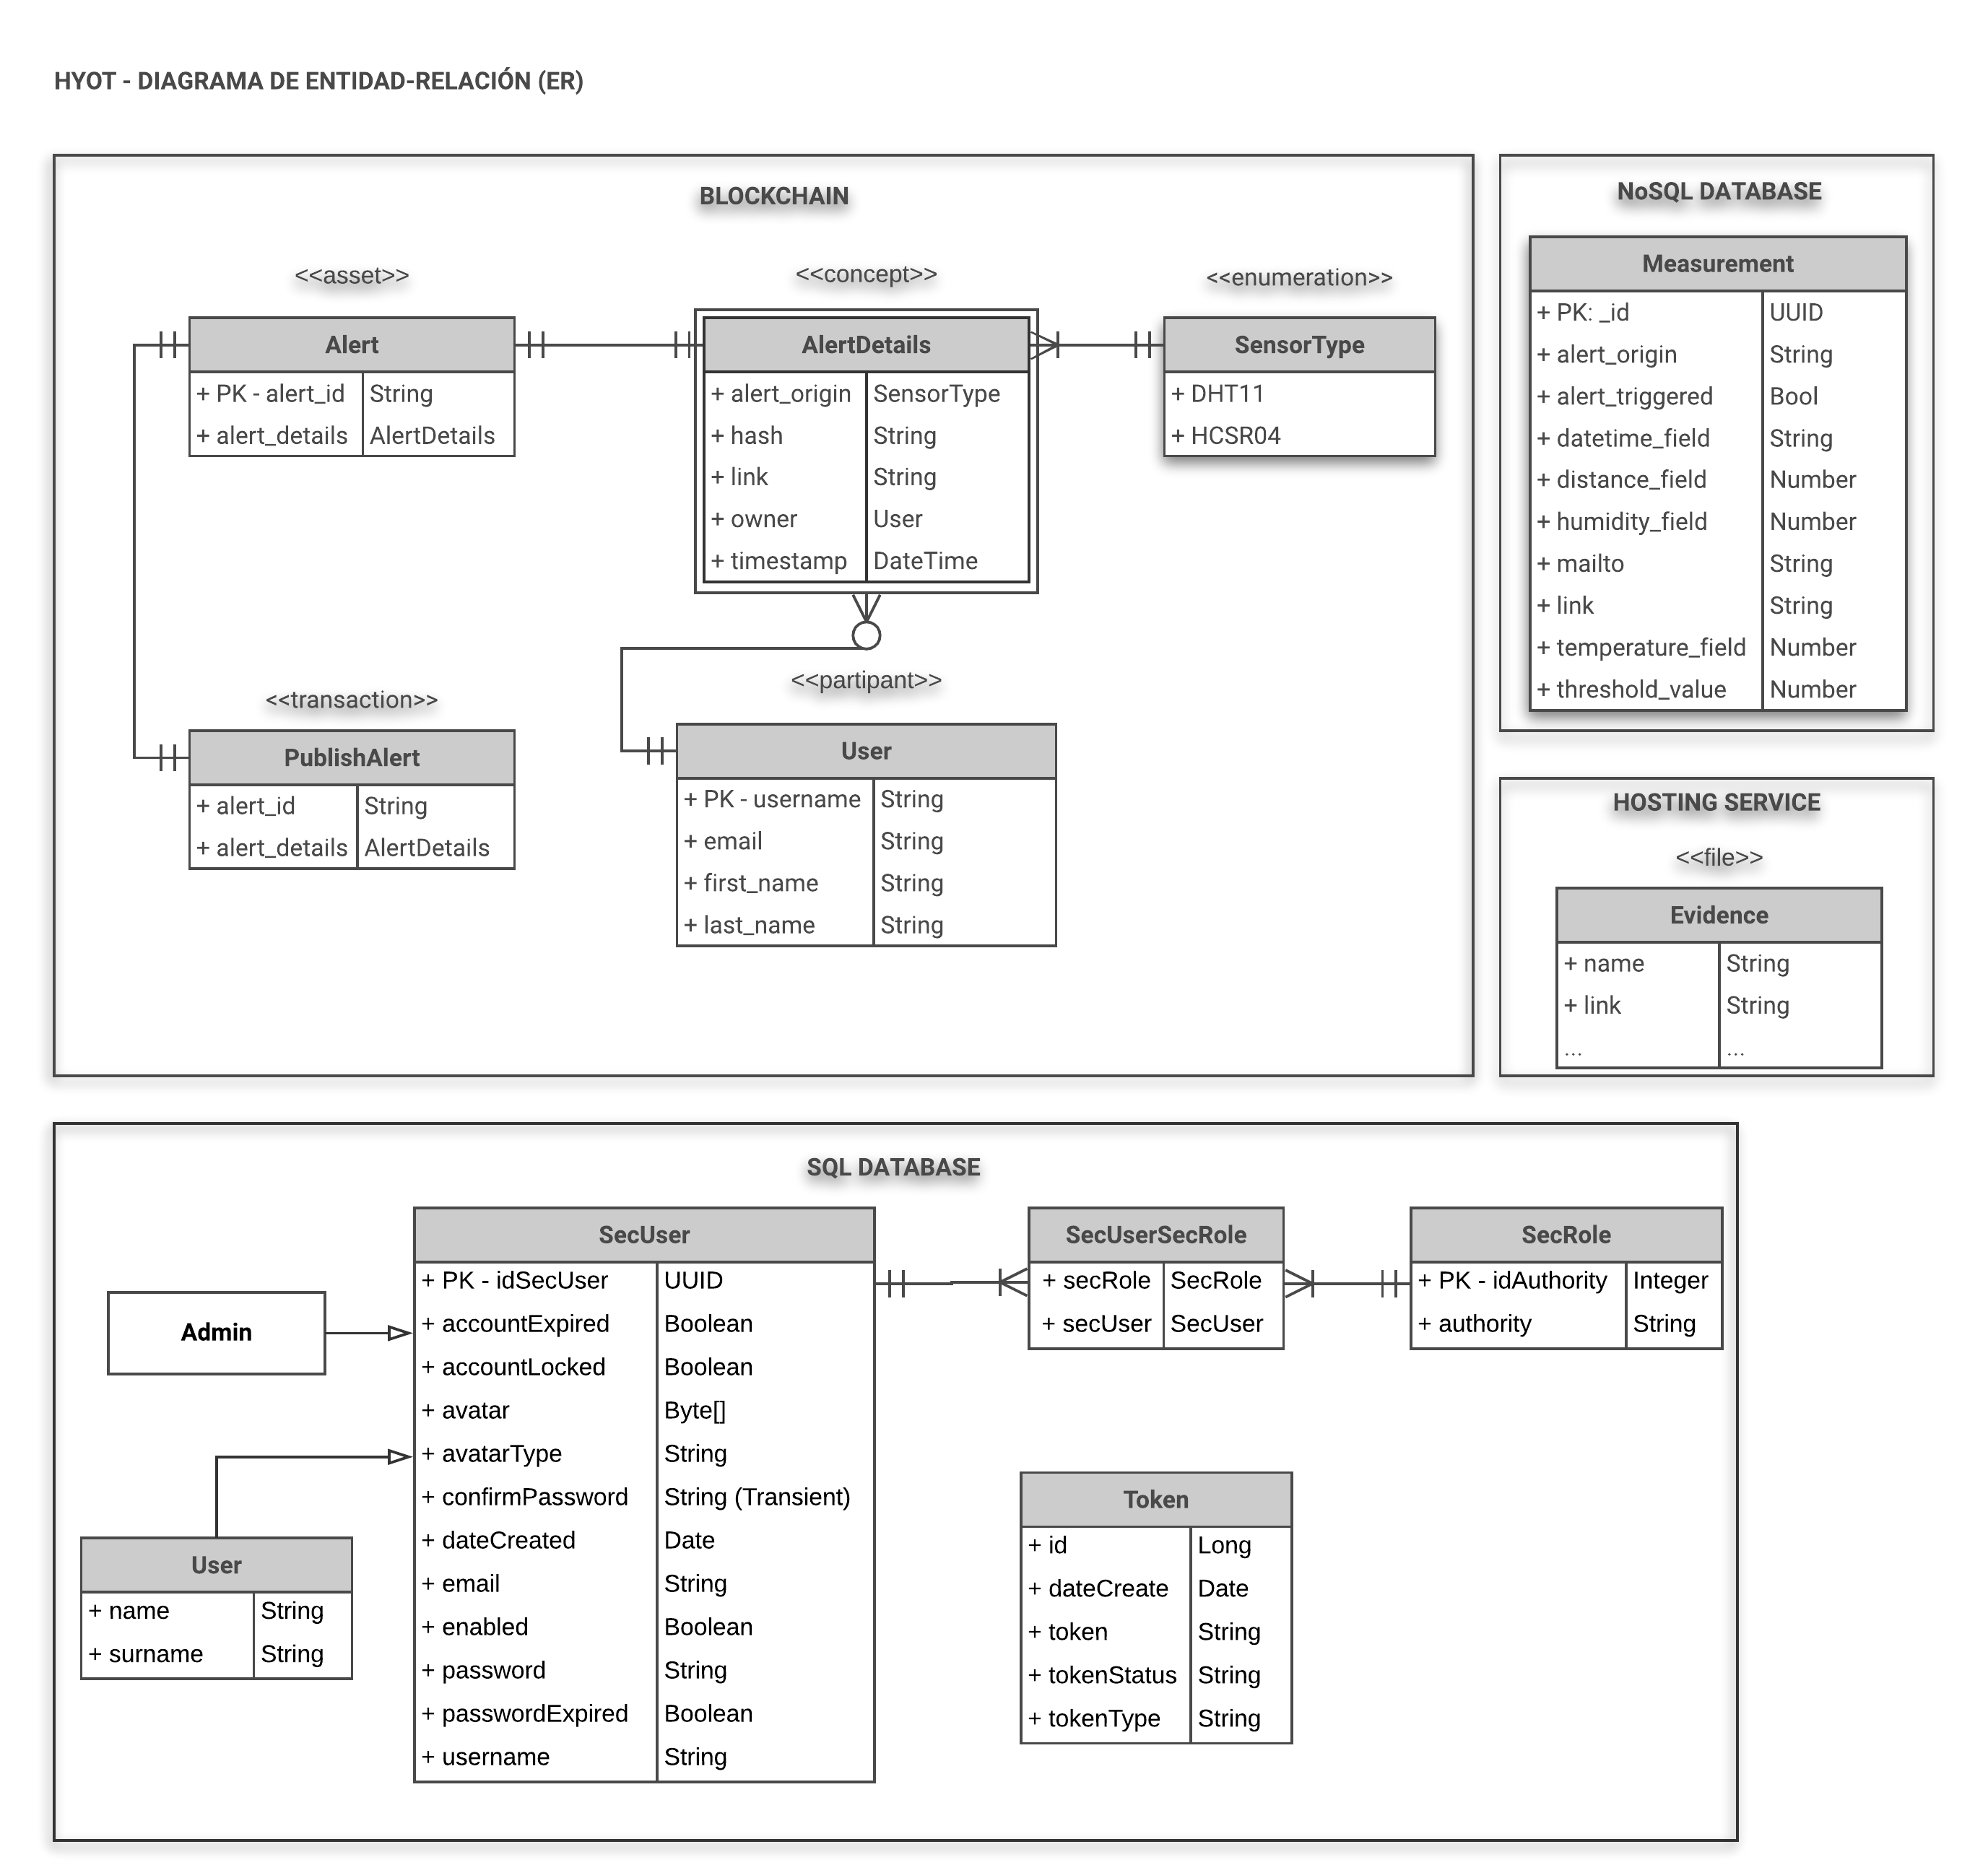
\includegraphics[width=18cm,height=9cm]{Images/design/p_er} \\
			\label{fig:design_er} 
		\end{center}  
	\end{figure}
	
	% Subsubsection
	\subsubsection{Diagrama de Estructura de Datos}
	
	El diagrama de Estructura de Datos es un modelo conceptual del sistema similar a los diagramas Entidad-Relación con la salvedad de que se centran en las relaciones de los elementos dentro de las entidades, en lugar de las relaciones entre las entidades mismas. \\
	
	La Figura \ref{fig:design_dsd} muestra el diagrama para el proyecto Hyot donde al igual que en el diagrama Entidad-Relación las entidades están categorizadas según el mecanismo de persistencia al que pertenecen. En este diagrama la particularidad, como su definición indica, se observa en las relaciones donde son los propios atributos los que marcan la relación. El significado que se le ha querido proporcionar a este diagrama en Hyot, es mostrar qué campos son utilizados en cada entidad y cuáles de ellos son compartidos entre diferentes entidades aunque la entidad en sí no esté relacionada, como es el caso de la entidad débil \texttt{AlertDetails} y la entidad \texttt{Measurement} donde no existe una relación explícita en el modelo pero ambas entidades comparten dos atributos que para la misma instancia poseerán el mismo valor.
	
	\begin{figure}[!ht]   
		\caption{Hyot - Diagrama de Estructura de Datos.} 
		\begin{center} 
			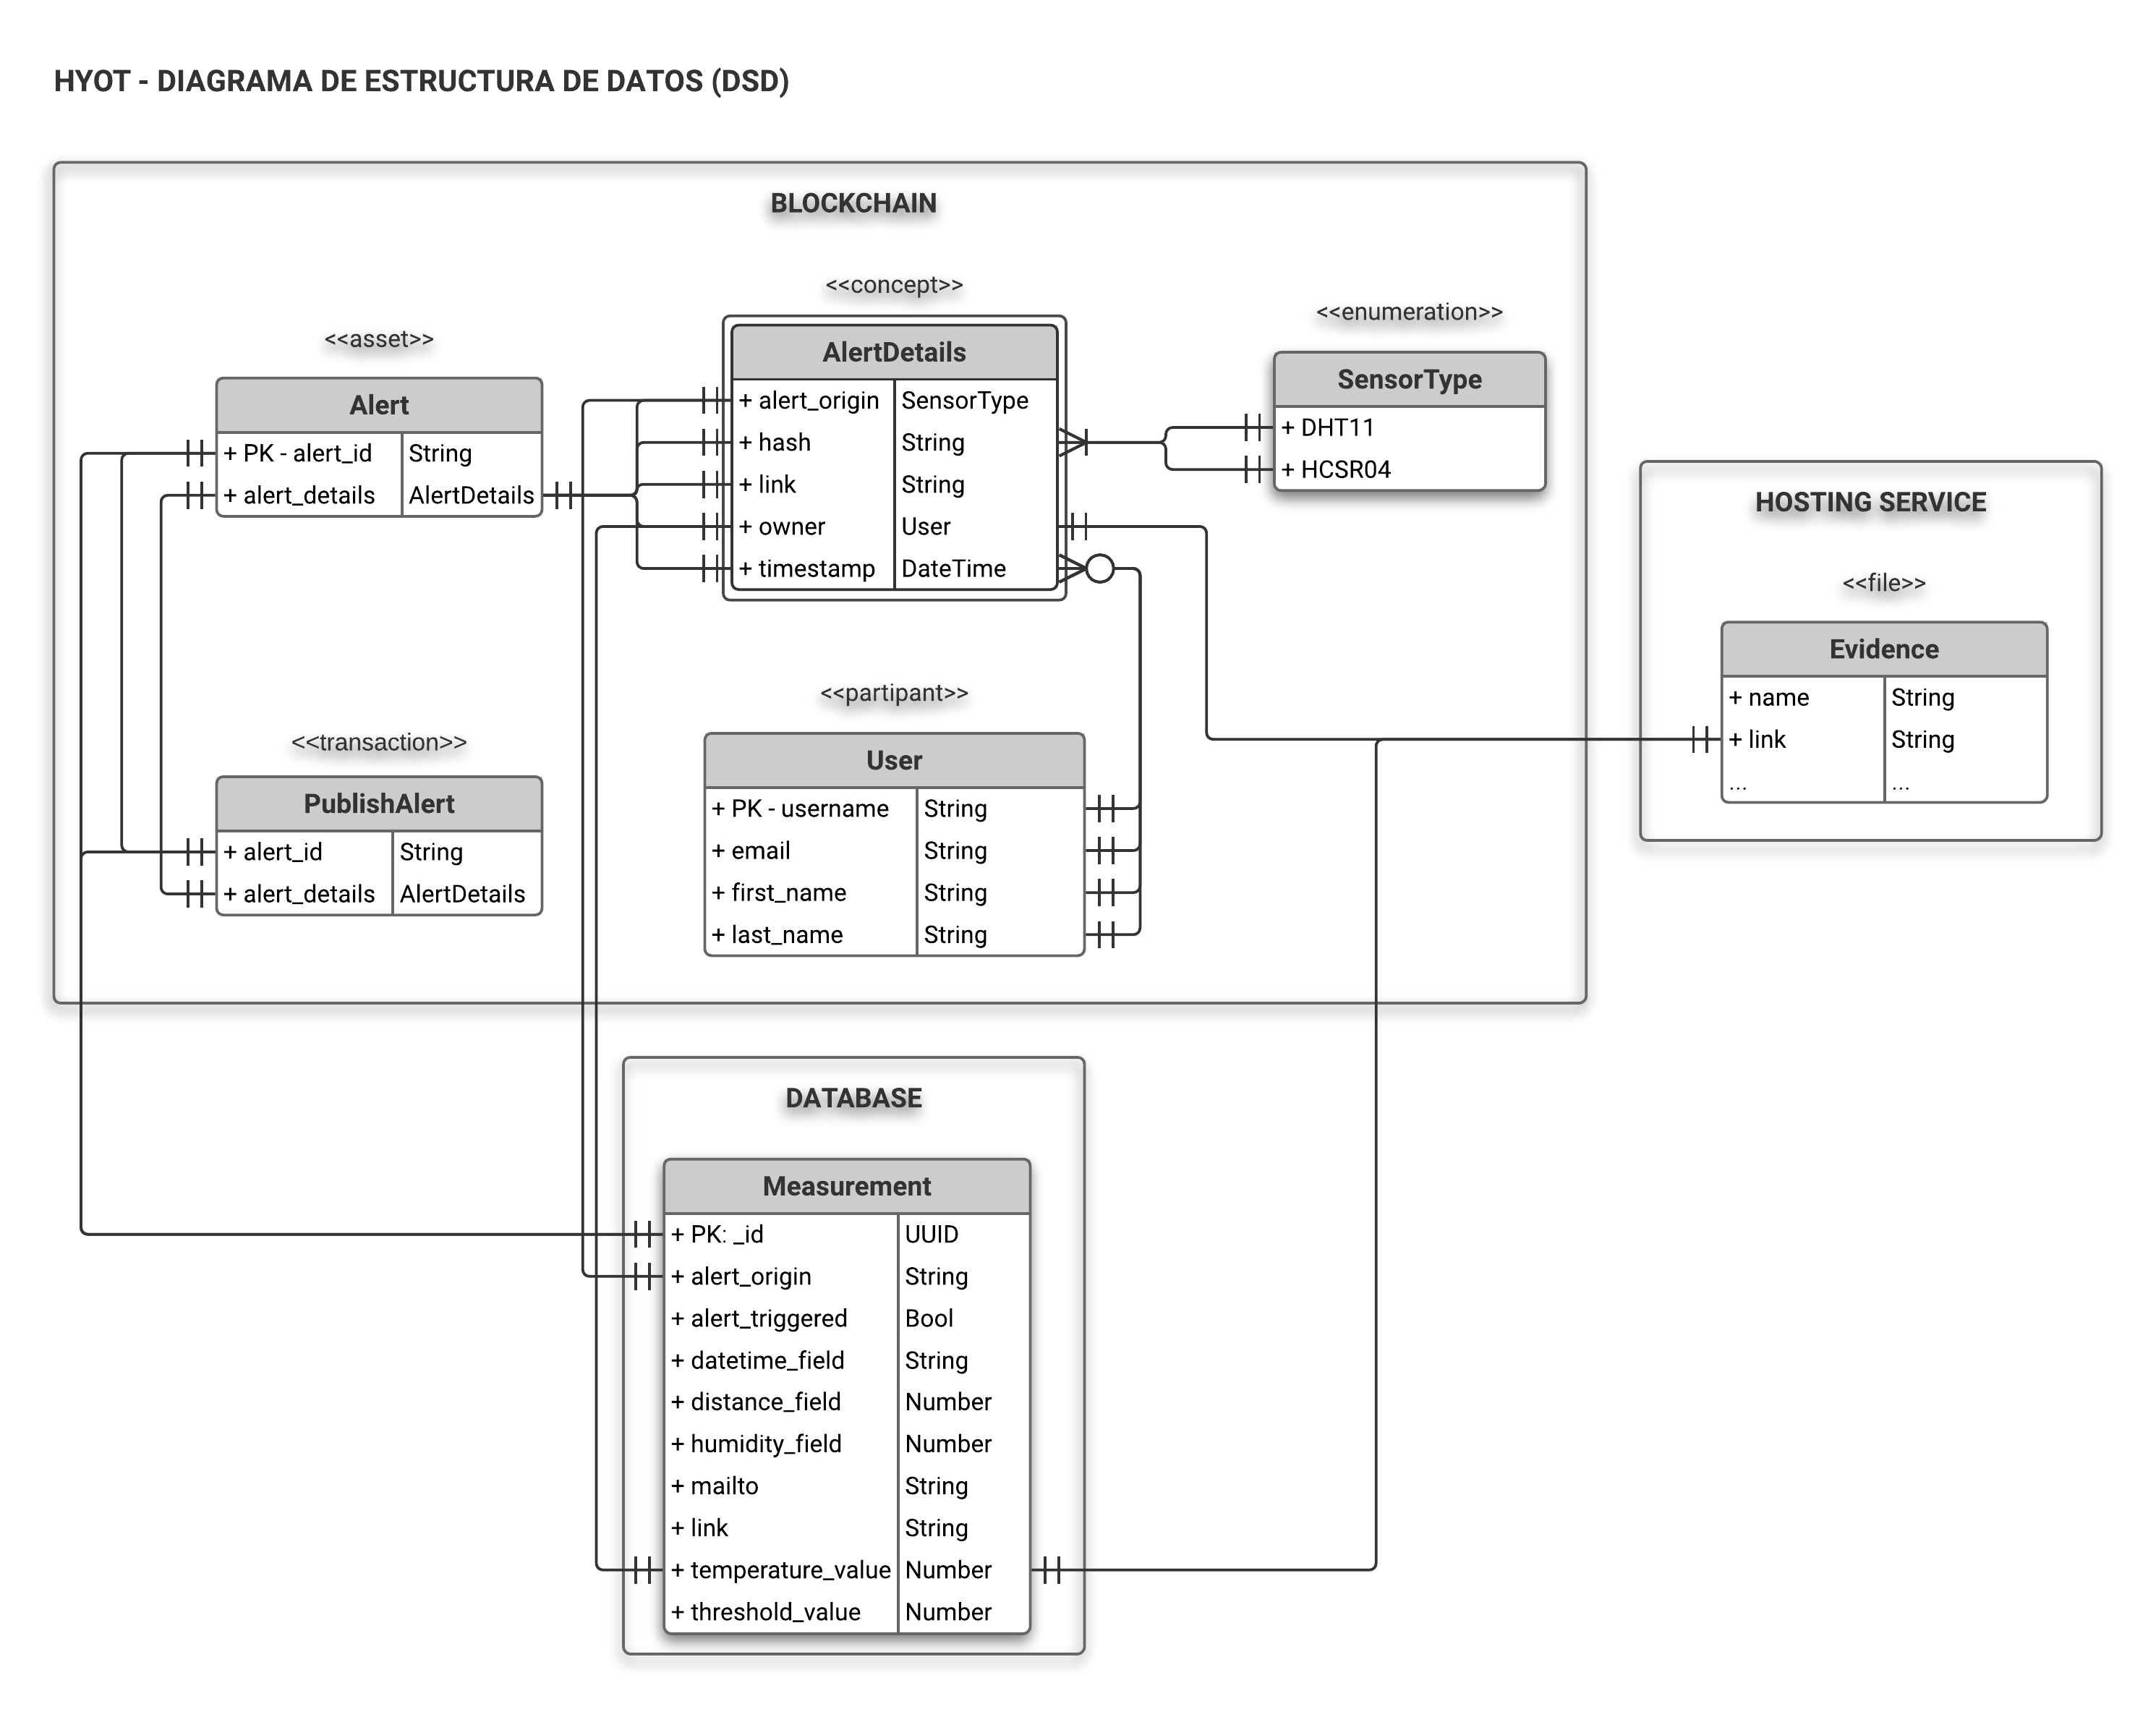
\includegraphics[width=17cm,height=10cm]{Images/design/p_dsd} \\
			\label{fig:design_dsd} 
		\end{center}  
	\end{figure}

	% Implementation
	\chapter{Implementación} \label{implementationChapter}
	
	\textbf{Resumen:} \textit{Todo sistema software se encuentra respaldado por un trabajo previo que lo conforma. Un aspecto importante es mostrar al lector la información interna más destacada sobre la implementación tecnológica llevada a cabo ya que de esta manera podrá conocer de una forma más concreta los entresijos del sistema, la funcionalidad, etc.}
	
	% Section
	\section{Hyot}
		
	Hyot es la prueba de concepto (\textit{\gls{poc}} -\gls{poc-a}-) de código abierto\footnote{Consulte el anexo \ref{install}. \nameref{install} para saber cómo conseguir el código.} desarrollada para llevar a cabo la trazabilidad de un entorno controlado de \gls{iot-a} (\textit{\gls{iot}}) mediante la tecnología \gls{hyperledgerfabric} (\gls{hyperledgerfabric-a}). Si bien es cierto que esta trazabilidad se puede realizar utilizando metodologías tradicionales, como son bases de datos o ficheros de \textit{logs} para almacenar la información, también es evidente que se carece de una falta de seguridad y garantía de que esta información ha perdurado inmutable desde su registro. \\
			
	Aprovechando el respaldo de todas las ventajas que proporciona el concepto de \Gls{blockchain} (\gls{blockchain-a}), Hyot mantiene parte de su persistencia en una \gls{blockchain-a} de carácter permisionada lo cual incrementa favorablemente la seguridad frente a las públicas ya que se puede controlar quién puede acceder y con qué privilegios al existir varios niveles de privacidad y de membresía proporcionando así mayor confidencialidad. De esta forma, la información no es expuesta públicamente a cualquier usuario ajeno a la misma y siempre estará identificada al participante que la añadió al registro por lo que favorece la trazabilidad de los datos. Pero solamente una parte de toda la información trazada del entorno es registrada en la \gls{blockchain-a}, en concreto aquella que interesa salvaguardar de una posible alteración ya que es la que proporcionará el resguardo y la prueba de que un suceso irregular realmente sucedió en un marco temporal. El suceso registrado -evidencia- en sí se guarda en una tercera parte de confianza (\gls{tpc-a}), como puede ser un servicio de almacenamiento en la nube, debido a su tamaño y al formato que presenta -fichero de vídeo-. Este agente externo puede no encontrarse 100\% securizado por lo que la evidencia almacenada debe ser protegida mediante el cifrado de su contenido y posterior firmado. La encriptación proporciona al contenido una codificación de tal manera que la información no sea legible de forma directa otorgando así confidencialidad y privacidad. Por su parte, el firmado ayuda a asegurar:
	
	\begin{itemize}
		\item Integridad de los datos: la evidencia no ha sido alterada de su forma original.
		\item Mensaje de autenticación o prueba de origen: la evidencia en realidad procede del supuesto remitente.
		\item No repudio: el emisor no puede negar la autenticidad de la evidencia que enviaron y firmaron con \gls{gpg-a} (\textit{\gls{gpg}}).
	\end{itemize}
		
	El resto de información que es meramente informativa y permite ampliar el contexto de la trazabilidad efectuada es almacenada en una base de datos (\gls{bbdd-a}). También, cabe destacar que es fácilmente escalable a ampliar a un mayor rango de cobertura en cuanto a \gls{iot-a} se refiere, indistintamente de usar dispositivos del mismo tipo o variedad en ellos. \\
	
	Esta solución, que es altamente configurable por el usuario mediante una inicialización preliminar, gestiona de forma transparente para el usuario una serie de sucesos -temperatura, humedad y distancia- del entorno que son monitorizados constantemente con una frecuencia por defecto de 3 segundos y en tiempo real desde fuentes de entradas de datos, como son los \glspl{sensor}, conectados a un ordenador de placa reducida (\textit{\gls{sbc}} -\gls{sbc-a}-) como es la \gls{raspberry} (\gls{raspberry-a}), siendo la última versión disponible (versión 3) la utilizada en el proyecto. Esta información recogida es analizada para determinar si es un instante concreto de tiempo los valores leídos son anómalos o no y por tanto decretar si en el entorno se está produciendo un acontecimiento desautorizado. En todo momento, las acciones ejecutadas y las mediciones efectuadas se notifican al usuario tanto a través del terminal como a través de los dispositivos de salida con los que cuenta el \gls{prototipo} \textit{hardware}\footnote{Consultar los anexos \ref{prototype}. \nameref{prototype} y \ref{prototypeGPIO}. \nameref{prototypeGPIO} para obtener más información sobre la implementación \textit{hardware} de Hyot.}, como son los \glspl{lcd-a} (\textit{\gls{lcd}}) y el \gls{led-a} (\textit{\gls{led}}), el cual se activa solamente en caso de accionar el protocolo de alerta. \\		 
			
	En el caso de que la medición actual no reporte ningún caso extraño, únicamente se realizan dos acciones: 
	
	\begin{enumerate}
		\item Almacenar la medición en la \gls{bbdd-a} para que quede constancia de que en ese momento temporal el entorno controlado no presenta ninguna incidencia. Para cada medición, se almacenan los siguientes campos:
		
			\begin{itemize}
				\item Identificador de la medición.
				\item Marca temporal (\textit{timestamp}) en la que ocurrió el suceso.
				\item Valor de la temperatura en la medición actual.
				\item Valor de la humedad en la medición actual.
				\item Valor de la distancia en la medición actual.
				\item Indicación de si se produjo un suceso anómalo y se activo el protocolo de alerta.
				\item Sensor y evento que originó el protocolo de alerta.
				\item Umbral límite del evento que lanzó el protocolo de alerta.
				\item Link al servicio de almacenamiento en la nube donde se ubica la evidencia encriptada y firmada.
				\item Dirección \textit{email} del destinatario para la notificación de la alerta.
			\end{itemize}
				
		\item Subir determinada información de la medición a una plataforma de \gls{iot-a} que actúa como pasarela de comunicación en tiempo real entre los dispositivos conectados y las aplicaciones que consumen los datos.		
	\end{enumerate}
	
	Por contra, si la lectura actual de valores presenta datos infrecuentes que superan unos umbrales preestablecidos considerados como posible indicio de una incidencia en el entorno, el procedimiento a seguir es más exhaustivo debido a que esta situación es la se quiere certificar que ha sucedido. Una incidencia no es sino una acción no controlada que tiene lugar en el entorno que se está vigilando, y origina la ejecución de un protocolo de alerta que comprende:
	
	\begin{enumerate}
		\item Captura de un vídeo -por defecto 10 segundos de duración- a través de una cámara (dispositivo Picamera) conectada a la \gls{raspberry-a} que representará la evidencia
		\item Cálculo del valor \textit{hash} del contenido de la evidencia, aplicando la última \gls{hash} \gls{sha-a}-3 definida (anteriormente conocido como \textit{keccak}), que actuará como prueba de integridad y se almacenará únicamente en la \Gls{blockchain}. 
		\item Encriptación y firmado de la evidencia con la utilidad \gls{gpg-a} puesto que se ha asumido un modelo de confianza nula en el cual toda la información debe ser protegida.
		\item Almacenamiento en la nube de la evidencia (p. ej. Dropbox). Este tipo de servicios son considerados \gls{tpc-a} que pueden poner en riesgo la privacidad de las evidencias, por lo que es necesario el paso anterior de cifrado y firmado.
		\item Volcado de la incidencia con información adicional (sensor de la alerta, umbrales de alerta, link apuntado al vídeo en la nube, etc.) en la \gls{bbdd-a} para que quede constancia de que en ese momento temporal el entorno vigilado presentó una lectura no controlada. En este método de almacenamiento se guardan los mismos campos mencionados anteriormente y como no garantiza la no alteración, la propiedad de prueba (código \textit{hash}) no es almacenada.
		\item Subida de determinada información de la medición a una plataforma de \gls{iot-a} que actúa como pasarela de comunicación en tiempo real entre los dispositivos conectados y las aplicaciones que consumen los datos.
		\item Registro de la incidencia	en \gls{hyperledgerfabric-a}. El punto central de Hyot es garantizar que el registro de un suceso anómalo no ha sido indebidamente modificado, de forma que una vez registrada una incidencia se tenga total certeza respecto a su integridad y veracidad. Este objetivo se consigue con esta tecnología, ya que proporciona un protocolo de consenso distribuido para la protección de integridad y un control de acceso que permite identificar a los agentes que introducen datos en la \Gls{blockchain-a}. En el dominio de nuestro caso de uso, se establecen los roles y permisos de los participantes (\textit{\glspl{participant}}), las transacciones (\textit{\glspl{transaction}}) posibles a ejecutar junto con el activo (\textit{\glspl{asset}}) \texttt{Alert} el cual contiene los siguientes atributos: 
		
				\begin{itemize}
					\item Identificador de la medición -en este caso también a la alerta-. Coincide con el identificador almacenado en la \gls{bbdd-a}.
					\item Marca temporal (\textit{timestamp}) en la que ocurrió el suceso. Coincide con la marca temporal almacenada en la \gls{bbdd-a}.
					\item Sensor que originó el protocolo de alerta.
					\item Código \textit{hash} del contenido de la evidencia sin encriptar.
					\item Link al servicio de almacenamiento en la nube donde se ubica la evidencia encriptada y firmada. Este activo, que también coincide con el almacenado en la \gls{bbdd-a}, evita la dependencia de acceso y de poseer permiso de acceso a la \gls{bbdd-a}.
					\item Participante que ejecutó la transacción de publicación de una nueva alerta.
				\end{itemize}

		\item Notificación del suceso no controlado al usuario administrador del sistema mediante el envío de un \textit{email} a la dirección de correo electrónico destino configurada, adjuntando la evidencia encriptada y firmada. Esta comunicación es importante para que el usuario puede conocer el estado del entorno en todo momento lo antes posible y ver que está sucediendo y poder tomar decisiones en caso necesario.
	
	\end{enumerate}
		
	La Figura \ref{fig:hyot_flow} muestra el mapa de flujo de forma superficial de la monitorización de sucesos del entorno en Hyot donde durante su ejecución, indistintamente de la activación o no del protocolo de alerta, se gestiona exhaustivamente cualquier error que se pueda producir, finalizando la ejecución de manera instantánea y notificando al usuario por la interfaz de la terminal. Además, si el error se produce durante la etapa de monitorización de sucesos el usuario de Hyot tendrá la certeza de que si algo no funciona correctamente se le notificará instantáneamente mediante el envío de un \textit{email} adjuntando el \textit{log} con los pasos ejecutados hasta el momento.
	
	% NEW PAGE
	\newpage
	
		\begin{figure}[!ht]   
			\caption{Diagrama de flujo - Monitorización de sucesos del entorno.} 
			\begin{center} 
	 			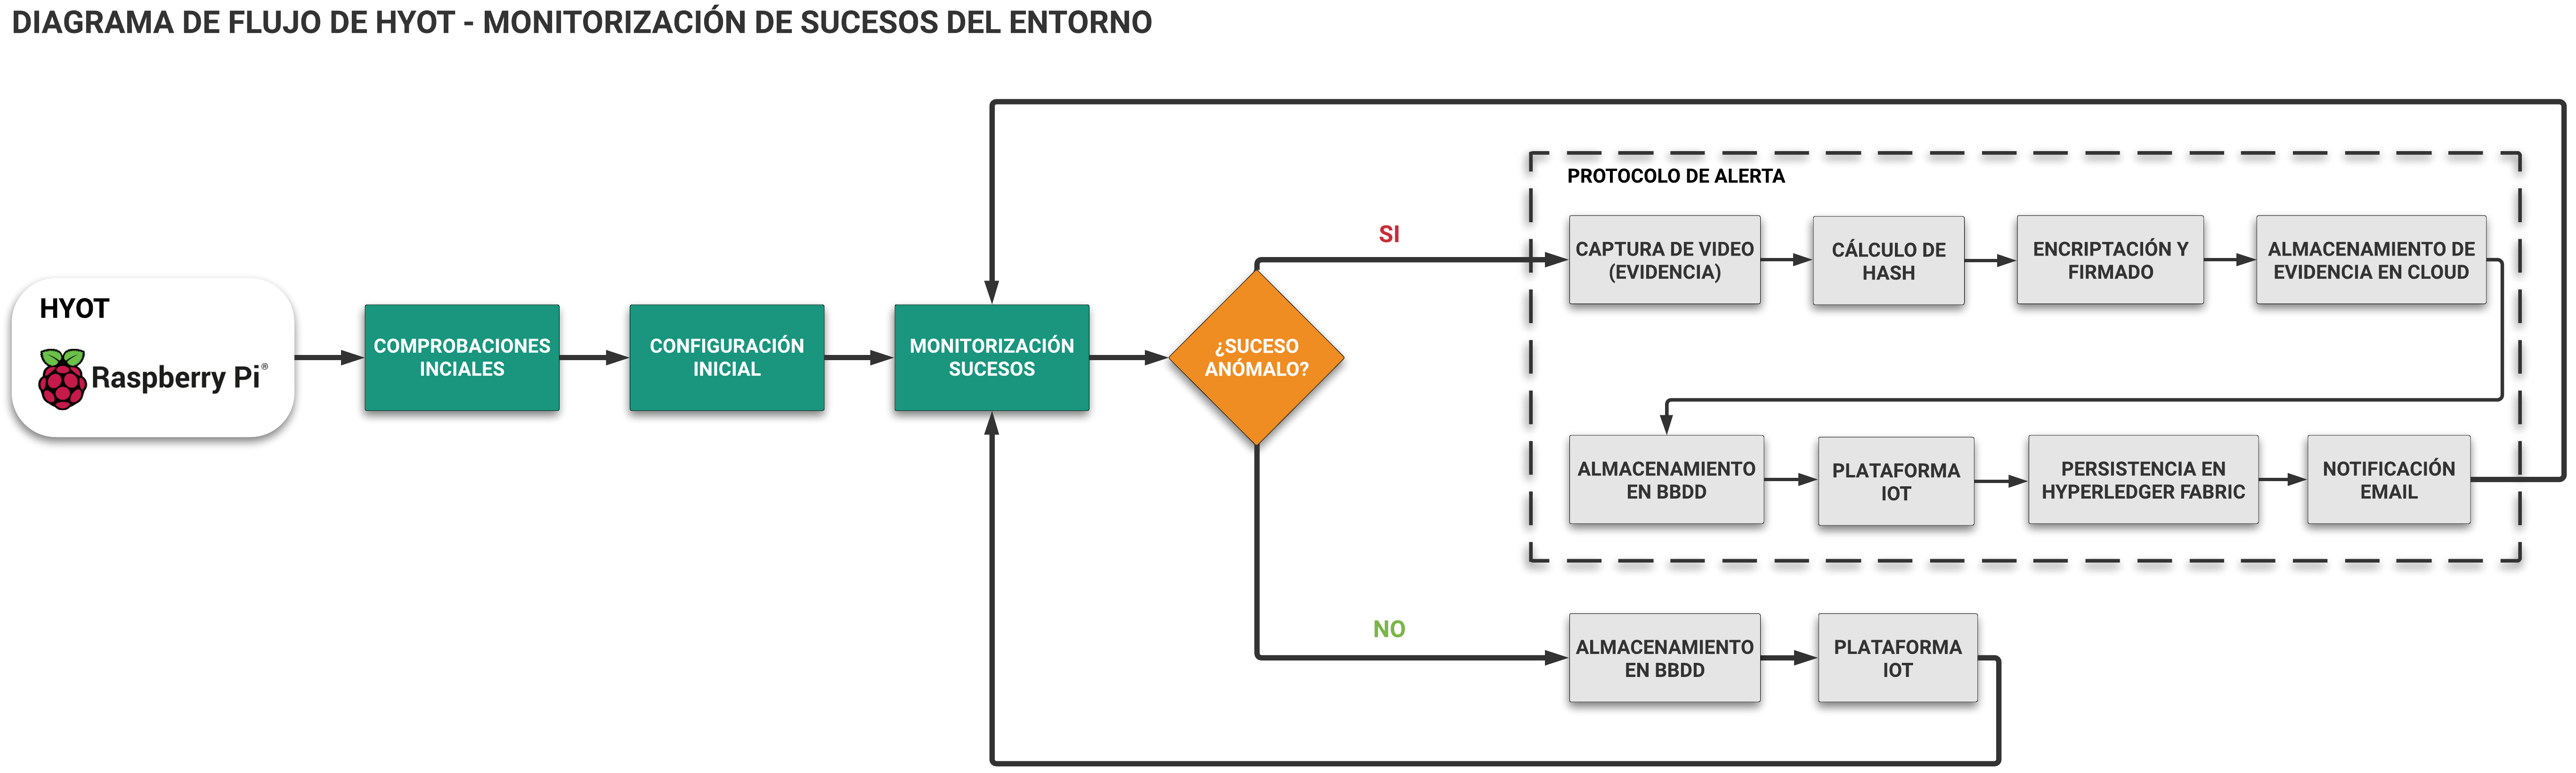
\includegraphics[width=18cm,height=6.7cm]{Images/implement/hyot_flow} \\
				\label{fig:hyot_flow} 
			\end{center}  
		\end{figure}

	A modo resumen, se puede detallar que Hyot se compone de tres componentes principales:

	\begin{itemize}
  		\item Componente de monitorización de sucesos del entorno a través de \glspl{sensor} situados en una \gls{raspberry-a}.
  		\item Protocolo de registro de incidencias en la \gls{blockchain-a} de \gls{hyperledgerfabric-a}, y almacenamiento de evidencias en la nube. 
  		\item Sistema web que actúa como cliente y consume en tiempo real la información registrada por la \gls{raspberry-a}.
	\end{itemize}

	A mayores de los componentes principales, dos componentes adicionales son ofrecidos con el fin de completar el proyecto y facilitar las tareas de:

	\begin{itemize}
  		\item Configuración inicial de la \gls{raspberry-a} para la posterior ejecución del componente de monitorización de sucesos del entorno. La Figura \ref{fig:hyot_setupflow} muestra el mapa de flujo de forma superficial de este proceso, donde se han omitido acciones y/o comprobaciones de menor importancia  y la gestión de errores por simplicidad, en cuyo caso de reproducción se finaliza la ejecución de manera instantánea notificando al usuario por la interfaz de la terminal.
  		
  		\item Desencriptación de evidencias previamente encriptadas y firmadas con \gls{gpg-a}. En este proceso, además de mostrar la firma, se verifica la integridad de su contenido a través de la comparación del valor \textit{hash} calculado sobre el contenido de la evidencia tras su descifrado y el valor \textit{hash} que inicialmente se había almacenado en la \gls{blockchain-a} cuando se produjo la incidencia. En este punto de comprobación reside la confianza que se depositó en esta tecnología ya que en caso de diferir los valores, se tiene la certeza de que la evidencia almacenada en la nube fue alterada. % TODO Mapa de flujo Revisar
	\end{itemize}
	
	\begin{figure}[!ht]   
		\caption{Diagrama de flujo - Configuración inicial de la \gls{raspberry-a}.} 
		\begin{center} 
	 		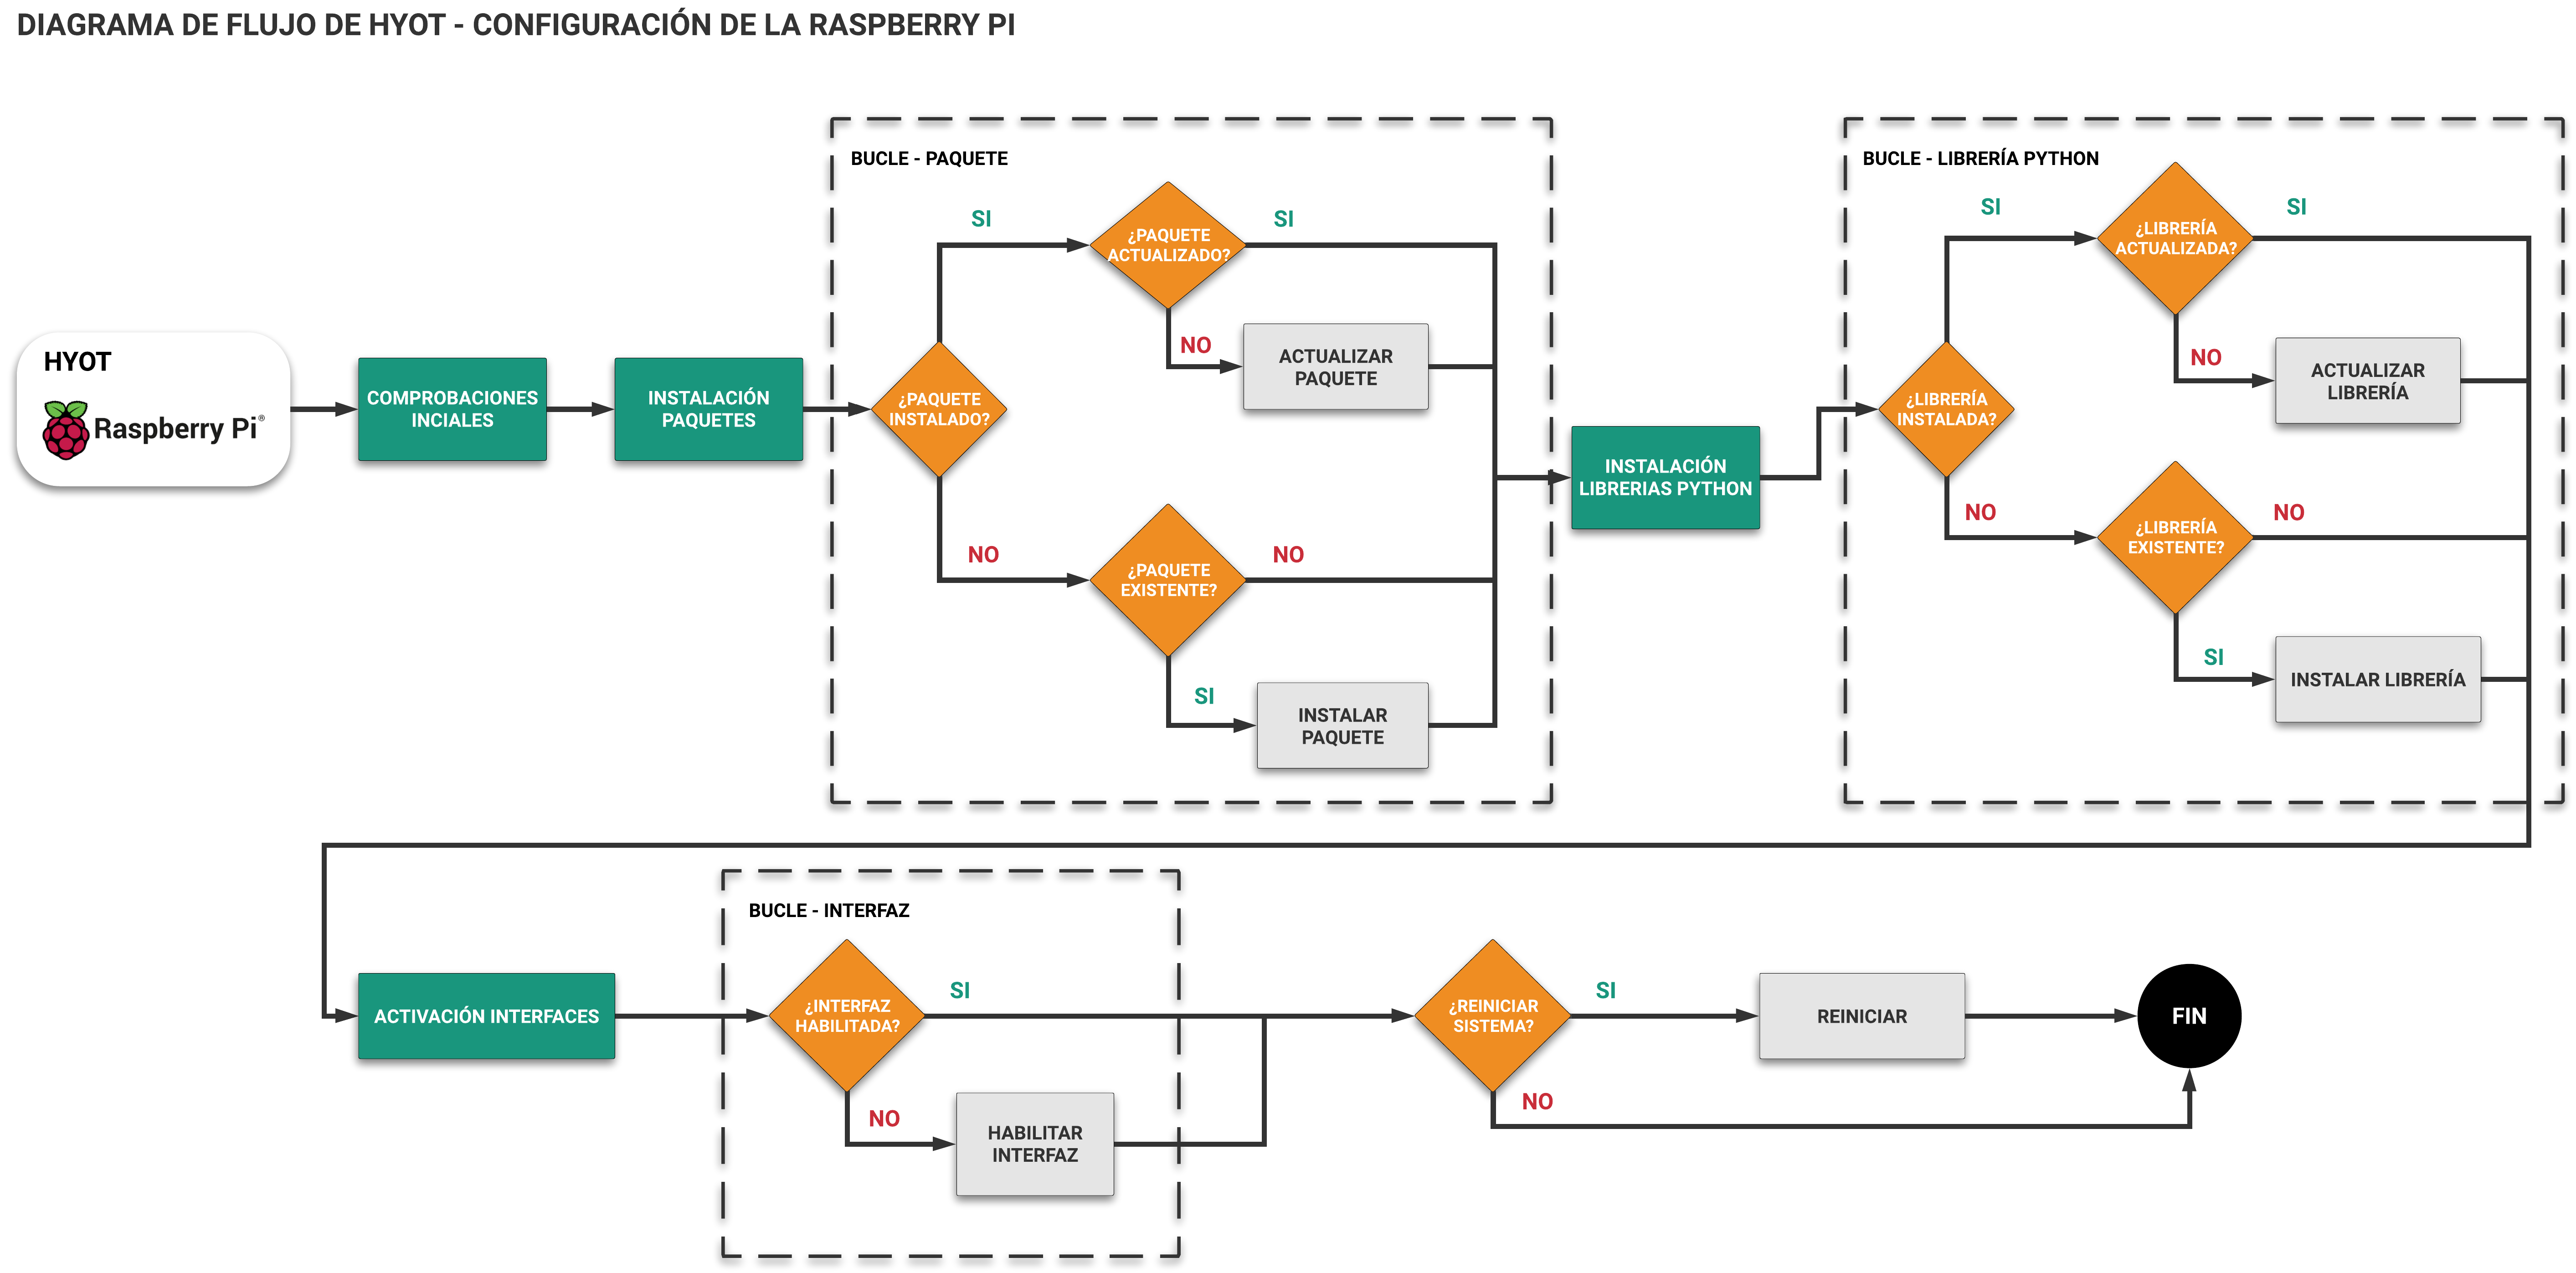
\includegraphics[width=17cm,height=9.3cm]{Images/implement/hyot_setupflow} \\
			\label{fig:hyot_setupflow} 
		\end{center}  
	\end{figure}
		
  	\begin{figure}[!ht]   
		\caption{Diagrama de flujo - Desencriptación de evidencias.} 
		\begin{center} 
	 		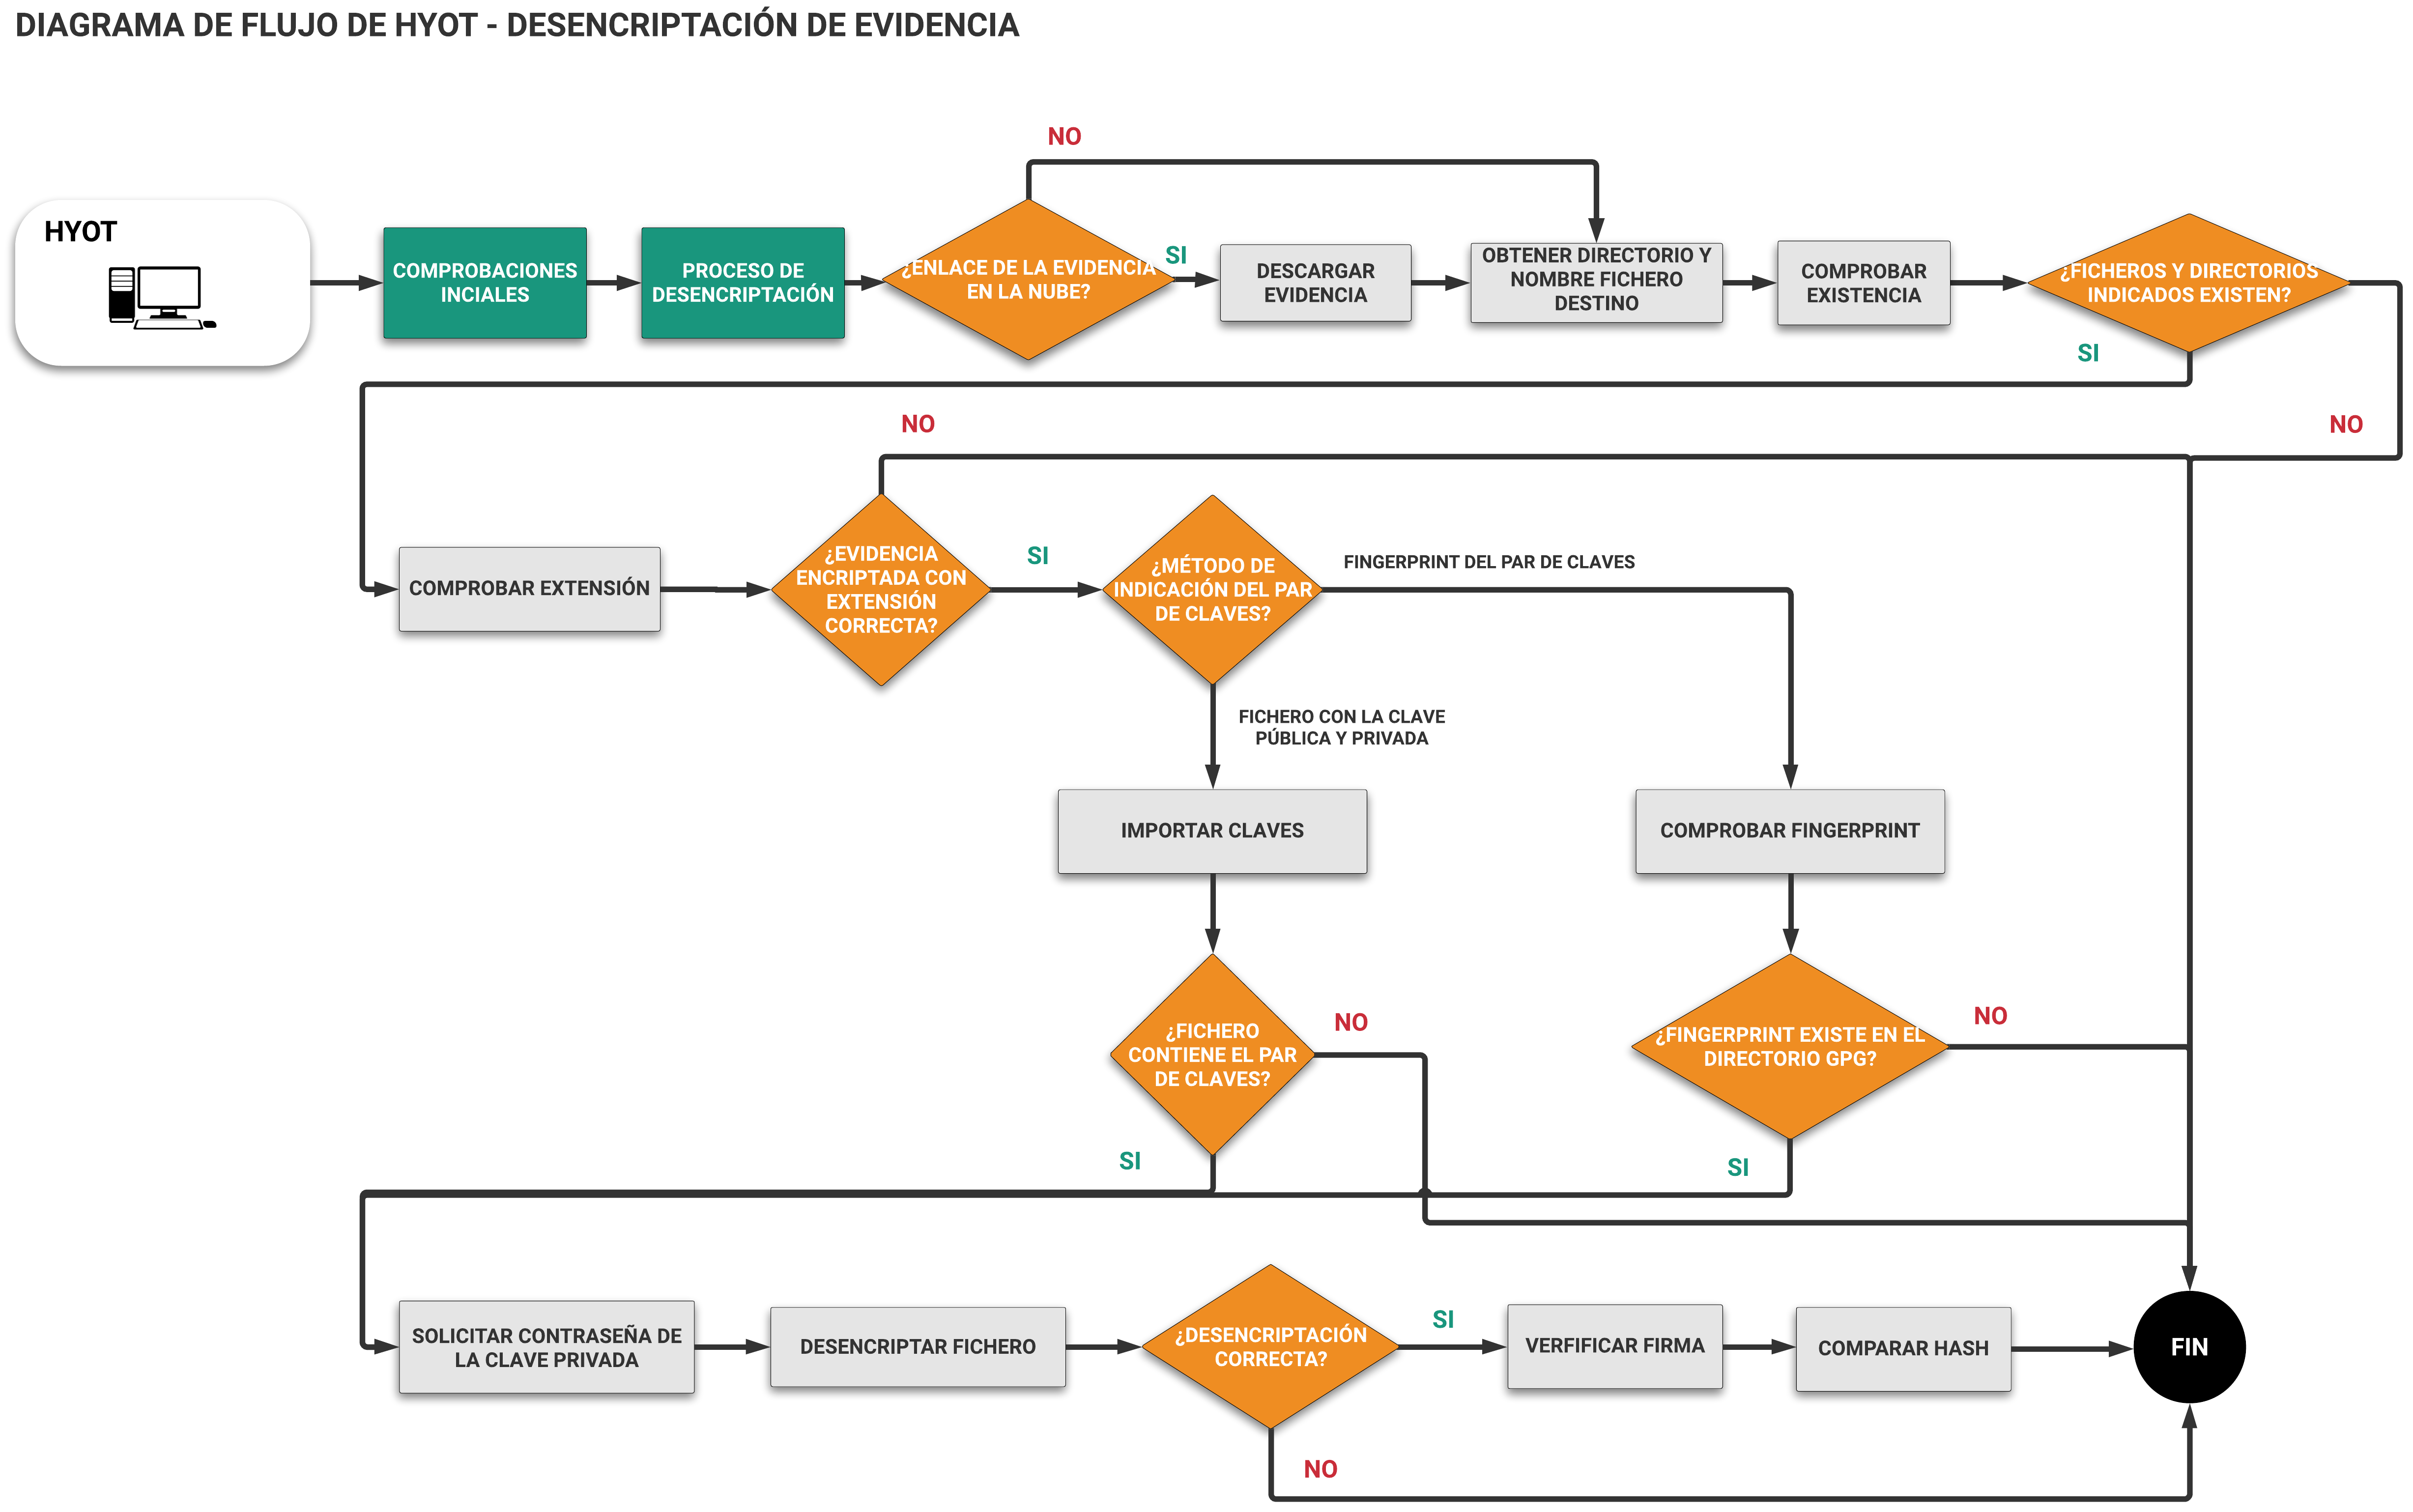
\includegraphics[width=18cm,height=9.2cm]{Images/implement/hyot_decryptionflow} \\
			\label{fig:hyot_decryptionflow} 
		\end{center}  
	\end{figure}
		
	% Section
	\section{Arquitectura de Hyot}
	
	La arquitectura de Hyot, mencionada anteriormente en la sección \ref{d_deployment}. \nameref{d_deployment}, se compone de 3 niveles y diferentes servicios y plataformas. En esta sección, se detallará de forma más completa esta disposición enfatizando y concretando las herramientas empleadas y desplegadas (Figura \ref{fig:hyot_architecture}).
	
		\begin{figure}[!ht]   
			\caption{Arquitectura de Hyot.} 
			\begin{center} 
	 			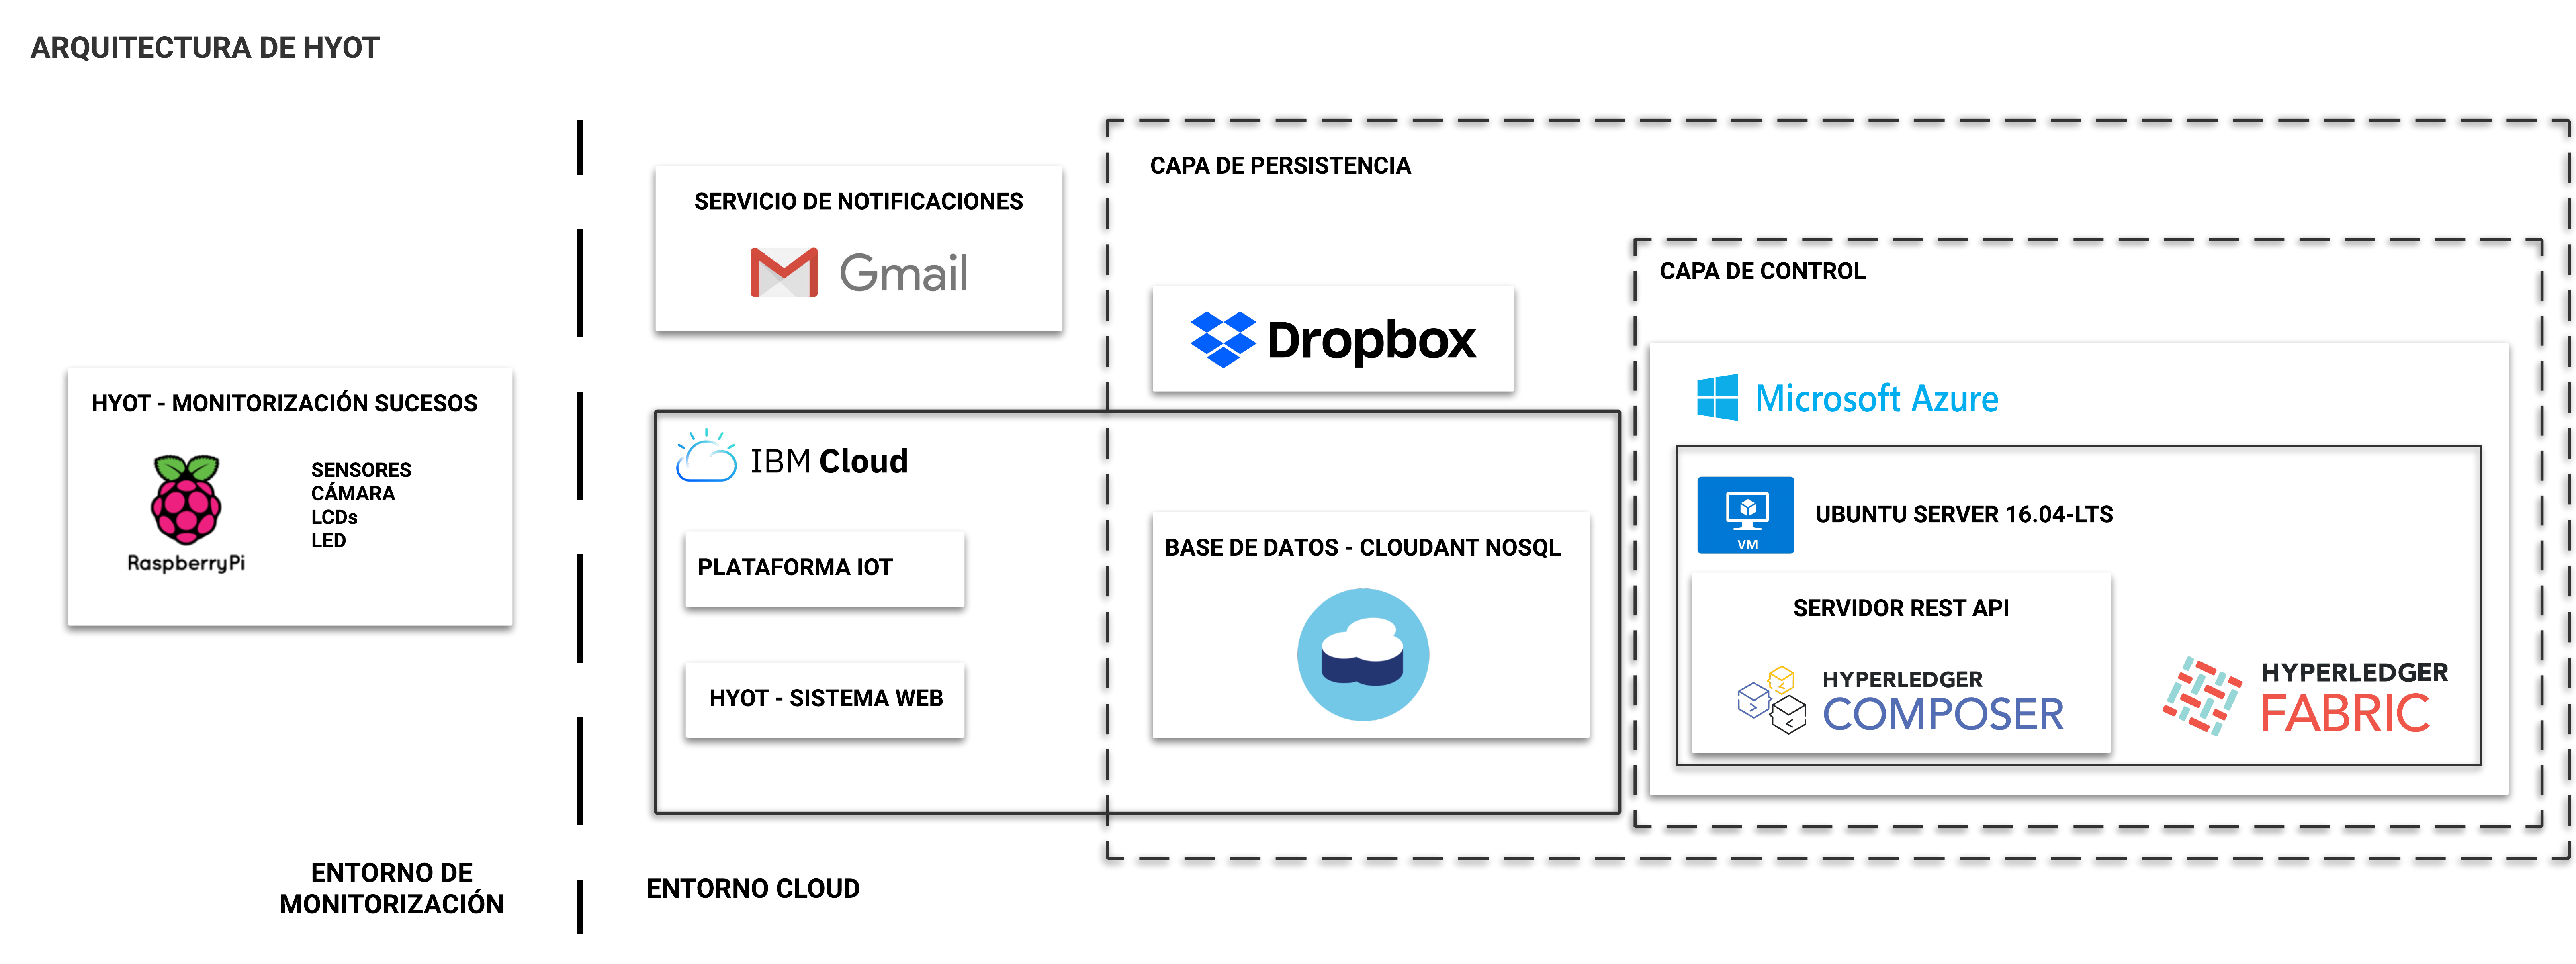
\includegraphics[width=18cm,height=10cm]{Images/implement/hyot_architecture} \\
				\label{fig:hyot_architecture} 
			\end{center}  
		\end{figure}
		
	Observando la arquitectura se diferencian claramente dos entornos donde los diversos componentes están desplegados:
	
	\begin{itemize}
		\item Entorno de ámbito local donde se despliega el componente de monitorización de sucesos del propio entorno. Se compone del prototipo \textit{hardware}\footnote{Consultar los anexos \ref{prototype}. \nameref{prototype} y \ref{prototypeGPIO}. \nameref{prototypeGPIO} para obtener más información.}: \gls{raspberry-a}, sensores, \gls{lcd-a}, \gls{led-a}, etc y se corresponde con el cliente pesado.
		\item Entorno en la nube donde se despliegan el resto de componentes principales de Hyot\footnote{Consulte los anexos \ref{install}. \nameref{install} y \ref{userguide}. \nameref{userguide} para obtener más información sobre la instalación y uso de estos componentes y servicios.} y servicios utilizados por éstos. Aquí, se puede diferenciar:
		% TODO Dependiendo de donde se indica la configuración de Gmail, Cloudant, platform IOT, IBM CLoud, etc. incluir el anexo o no en el footnote anterior.
		\begin{itemize}
			\item La capa de persistencia que engloba los tres mecanismos para persistir toda la información utilizada en Hyot.
			
			\begin{itemize}
				\item Por un lado, se encuentran la \gls{bbdd-a} como servicio (\textit{\gls{dbaas}} -\gls{dbaas-a}-) \gls{cloudant} la cual pertenece a su vez al servicio de IBM Cloud y el servicio de almacenamiento en la nube Dropbox (\textit{\gls{saas}} -\gls{saas-a}-) \cite{gonzalez:2011:TCCS}.
				
				\item Y por otro lado y dentro de la capa de persistencia, se encuentra la capa de control formada por el despliegue de la \gls{blockchain-a} permisionada. Esta denominación se debe a que la información aquí guardada permite controlar y garantizar la veracidad de la trazabilidad registrada. En este caso, se desplegó una (\textit{\gls{vm}} -\gls{vm-a}-) Ubuntu en el servicio Microsoft Azure con dirección IP: \texttt{40.121.15.202} y en dicha máquina se localiza \gls{hyperledgerfabric-a} y el servidor \gls{rest-a} (\textit{\gls{rest}}) \gls{api-a} (\textit{\gls{api}}) de \gls{hyperledgercomposer} (\gls{hyperledgercomposer-a}), el cual recibe peticiones securizadas por parte del sistema web y del componente de monitorización de sucesos e interactúa con la fábrica \gls{blockchain-a} de \gls{hyperledgerfabric-a}.				
			\end{itemize}  
		 				 		
			\item Los servicios desplegados en la nube pertenecientes a IBM Cloud, donde se localizan:
			
			\begin{itemize}
				\item La ya mencionada \gls{bbdd-a}.
				\item La plataforma como servicio (\textit{\gls{paas}} -\gls{paas-a}-) de \gls{iot-a} para enviar datos de forma sencilla desde dispositivos y permitir la comunicación entre éstos y las aplicaciones. 
				\item El sistema web, desarrollado en {\color{red}XX}, que actuará como cliente delgado para consumir la información. Esta aplicación es desplegada en el servicio de \gls{cloudfoundry}, considerado un \gls{paas-a}, de tal manera que se garantiza, con respecto a un sistema local, una rápida provisión y despliegue de la aplicación junto con una total disponibilidad. % TODO Indicar la tecnología y añadir la imagen en el Figura. Esa tecnología también debe ir en el diagrama de despliegue. Añadir la dirección web donde se puede acceder.
			\end{itemize}
			
			\item El servicio para el envío de notificaciones mediante \textit{emails}, siendo Gmail (\gls{saas-a}) el configurado y utilizado.
		\end{itemize}
	\end{itemize}
			
	% Section
	\section{Tecnologías de desarrollo}
	
	% TODO número de tecnologias 3? Añadir el web
	Comentadas ya tanto las herramientas \textit{software} en el punto \ref{tools}. \nameref{tools} como los servicios utilizados -sección anterior-, se pasa a presentar las tecnologías de desarrollo empleadas para la codificación y los componentes donde se utilizaron. En concreto, en Hyot se han empleado tres tecnologías para el desarrollo:
	
	\begin{itemize}
		\item GNU Bash \cite{bash}: es un intérprete y procesador de comandos de \textit{\gls{shell}} que permite ejecutar \textit{\glspl{script}} simples por consola con la finalidad de automatizar tareas que puede desempeñar un administrador de sistemas como puede ser la configuración de un sistema. Fue desarrollado para el proyecto GNU en el año 1987 como la versión libre del hasta entonces intérprete más importante de \gls{unix}: \gls{bourneshell} (\gls{bourneshell-a}) y actualmente es el estándar de todas las distribuciones \gls{gnulinux}. Esta tecnología ha sido usada para codificar el componente de configuración de la \gls{raspberry-a} debido a que es al no requerir un código demasiado complejo en cuyo caso hubiese que haber trabajo con otras tecnologías más potentes de \textit{scripting} como \gls{perl} o \gls{python}.
	
		% TODO – Sistema web
		\item Javascript (JS) \cite{javascript}: es un  lenguaje de programación ligero e interpretado -orientado a objetos, basado en prototipos, imperativo, débilmente tipado y dinámico, entre otras características- que surgió debido a la necesidad de ampliar las posibilidades de desarrollar sistemas web del lado del cliente (\textit{\gls{frontend}}) con contenido más complejo, dinámico y funcional ya que hasta entonces las prestaciones de estos sitios se encontraba limitada exclusivamente a funcionalidades básicas sobre los elementos de texto, estilos y formatos, es decir, a contenido estático. Iniciado originalmente por Brendan Eich de la compañía de \textit{software} Netscape Communications Corporation con el nombre de Mocha, el cual fue renombrado posteriormente a LiveScript, para finalmente quedar como JavaScript y continuado por la alianza entre Netscape y Sun, se ha popularizado enormemente hasta convertirse es un estándar basado en \gls{ecmascript} y soportado por todos los navegadores actuales. El uso de este lenguaje se ha centrado en el desarrollo de la red de negocio con la tecnología \gls{hyperledgercomposer-a} ya que es el lenguaje definido por defecto para describir la estructura de los recursos que participan en la \gls{blockchain-a}. Aun así, esta tecnología presenta su propia sintaxis basada en este lenguaje.
		
		\item Python \cite{python}: es un lenguaje de \textit{scripting} de código abierto interpretado, interactivo y orientado a objetos creado por Guido van Rossum, preparado para desarrollar independientemente de la plataforma y sistema operativo desde aplicaciones de escritorio, \textit{\glspl{script}} o incluso, sistemas web. En este tipo de lenguajes, que son más flexibles y portables que los lenguajes compilados, se emplea un programa intermedio llamado intérprete donde se traduce el código fuente a un pseudo código llamado \textit{bytecode} la primera vez que se ejecuta, generando archivos \texttt{.pyc} o \texttt{.pyo}, que son los que se ejecutarán en sucesivas ocasiones directamente en la computadora, en lugar de compilar el código a lenguaje máquina comprensible por este dispositivo. En los últimos años el lenguaje se ha hecho muy popular, debido a todas las características que proporciona. Debido a esto, a la facilidad de interacción con componentes electrónicos gracias a las librerías existentes y al contexto y necesidades -rapidez y sencillez de desarrollo junto con existencia de librerías auxiliares- de los componentes que se desarrollaron se ha usado para:
		
		\begin{itemize}
			\item El componente de monitorización de sucesos del entorno.
			\item El componente de desencriptación de evidencias previamente encriptadas  y firmadas con \gls{gpg-a}.
		\end{itemize}
	\end{itemize}
		
	% Section
	\section{Red de negocio de Hyperledger Composer} \label{businessNetwork}
	
	% TODO - Peer node?
	La especificación de la red de negocio es un concepto clave en \gls{blockchain-a} puesto que representa la digitalización de los elementos que la conforman junto con la lógica de negocio. En Hyot, se ha empleado la herramienta \gls{hyperledgercomposer-a} para la definición de esta red la cual es desplegada a través de un fichero \texttt{.bna} y mantenida por cada nodo conectado a la \gls{blockchain-a} de \gls{hyperledgerfabric-a}\footnote{En el contexto actual del Trabajo Fin de Máster (\gls{tfm-a}) y debido a las limitaciones existentes, la red estará formada por un único nodo, en concreto, aquel desplegado en \gls{hyperledgerfabric-a} de la \gls{vm-a} establecida en el servicio Microsoft Azure.}. Aunque \gls{hyperledgercomposer-a} no aprovecha aun todas las características que ofrece el \textit{\gls{framework}} \gls{hyperledgerfabric-a}, las necesidades actuales son cubiertas con creces con esta herramienta\footnote{\gls{hyperledgercomposer-a} se encuentra bajo constante desarrollo y respaldada por una fuerte comunidad de desarrolladores, hecho contrastado por la liberación constante de nuevas \textit{releases}. Consultar \cite{hyperledgercomposer:releases} para obtener más información.} y su uso se debe a los beneficios que proporciona:

	\begin{itemize}
		\item Simplificación del proceso de implementación de la \gls{blockchain-a} ya que abstrae al desarrollador de numerosos procesos y conceptos lo cuales son generados automáticamente a más bajo nivel al usar dicha herramienta.
		\item Aceleración de la creación de aplicaciones eliminando el esfuerzo requerido si se hiciese a un más bajo nivel de codificación -utilizando directamente \gls{hyperledgerfabric-a}-.
		\item Posibilidad de prueba de la definición de la red realizada antes de ser desplegada en un entorno de producción lo que ayuda a reducir riesgos.
	\end{itemize}
	
	La solución de la red de negocio construida es muy simple y se detalla a continuación para un pleno entendimiento. En primer lugar, se van a definir los conceptos claves que conforman una red los cuales corresponden a definiciones de clases instanciables:
	
	\begin{itemize}
		\item Activo o \textit{asset}: hace referencia a los bienes, servicios o propiedades tanto tangibles como intangibles que son almacenados en registros en la \gls{blockchain-a}. Dicho de otra forma, es cualquier cosa del mundo real que pueda ser representado y utilizado en una red de negocio.
		\item Participante: representa los miembros de una red de negocio los cuales poseen activos y envían transacciones para intercambiar activos o para modificar sus propiedades.
		\item Transacción: simbolizan las reglas de negocio permitidas, es decir, los procedimientos por el cual los participantes interactúan con los activos.
	\end{itemize}

	Para la red actual de Hyot -versión 1.0.0- se ha determinado el siguiente espacio de nombres \texttt{org.hyot.network.} y se ha definido únicamente un tipo de activo (estereotipo \texttt{<<asset>>}) con nombre \texttt{Alert} que representa la alerta de un suceso anómalo ocurrido en el entorno monitorizado. Este activo, que ha sido especificado utilizando a mayores un tipo enumerado y una clase abstracta\footnote{Indica que el tipo no puede ser instanciado.} \texttt{concept}\footnote{Clase que no representa ni un activo, ni un participante ni una transacción y típicamente son contenidos por alguno de ellos.} como objetivo meramente de aprendizaje\footnote{El foco también ha sido aprender la sintaxis disponible por lo que se que han definido propiedades que a priori no proporcionan valor.}, se compone de:
	
		\begin{itemize}
			\item Identificador de la alerta (tipo \texttt{String}).
			\item Clase \texttt{AlertDetails} con estereotipo \texttt{<<concept>>} que contiene los detalles de la alerta:
			
			\begin{itemize}
				\item Marca temporal (\textit{timestamp}) en la que ocurrió el suceso (tipo \texttt{DateTime}).
				\item Sensor que originó el protocolo de alerta de tipo \texttt{SensorType} el cual representa una enumeración.
				\item Valor \textit{hash} del contenido de la evidencia sin encriptar (tipo \texttt{String}).
				\item Link al servicio de almacenamiento en la nube donde se ubica la evidencia encriptada y firmada (tipo \texttt{String}).
				\item Participante que ejecutó la transacción de publicación de una nueva alerta de tipo \texttt{User}.
			\end{itemize}
			
			\item Enumerado con los nombres de los posibles sensores que pueden originar la alerta: DHT11 y HCSR04.
		\end{itemize}
		
	En cuanto a los participantes se ha definido al participante \texttt{User} (estereotipo \texttt{<<participant>>}) que representa el usuario o dispositivo que registra una alerta en la \gls{blockchain-a} y contiene las siguientes propiedades: 	
		
		\begin{itemize}
			\item Identificador de la alerta (tipo \texttt{String}).
			\item Clase \texttt{AlertDetails} con estereotipo \texttt{<<concept>>} que contiene los detalles de la alerta.
		\end{itemize}
		
	La lógica de negocio viene definida por la especificación de una transacción \texttt{PublishAlert} (estereotipo \texttt{<<transaction>>}) que contiene dos propiedades:
	
		\begin{itemize}
			\item Nombre de usuario (tipo \texttt{String}). Esta propiedad actuará como identificador único.
			\item Dirección \textit{email} (tipo \texttt{String}). Esta propiedad es opcional.
			\item Primer apellido (tipo \texttt{String}).
			\item Segundo apellido (tipo \texttt{String}).
		\end{itemize}
	
	% TODO - Querys completar
	Esta transacción es ejecutada por una función procesadora de transacciones (\texttt{publish}) cuya función es el registro de un nuevo activo \texttt{Alert} en la \gls{blockchain-a}. Además, en la red de negocio se pueden especificar las consultas (\textit{querys}) que se pueden ejecutar contra la \gls{blockchain-a} y definir los privilegios de acceso para los participantes y activos. Para el primer caso, se definió una consulta que permite obtener todas las alertas generadas por un determinado sensor. Con respecto a la lista de control de acceso, ésta contiene la siguientes reglas:
	
	\begin{itemize}
		\item Todos los participantes de tipo \texttt{User} pueden subir transacciones \texttt{PublishAlert}.
		\item Únicamente se crearán activos de tipo \texttt{Alert} cuando se suban transacciones \texttt{PublishAlert}, es decir, un nuevo activo \texttt{Alert} no puede ser creado directamente.
		\item Todos los participantes de tipo \texttt{User} pueden obtener el registro de los  activos \texttt{Alert} cuyo poseedor sean ellos mismos lo que implica que los registros una vez registrados no puedan ser modificados ni borrados proporcionando así una capa extra de seguridad al asegurar que si una alerta fue almacenada fue porque realmente sucedió. Esta regla además implica que un determinado participante \texttt{User} no puede ver los registros de alerta de otros participantes de este tipo.
		\item Todos los participantes poseen acceso a los recursos de sistema.
		\item Los administradores de la red de negocio presentan acceso completo a los recursos de usuario.
		\item Los administradores de la red de negocio presentan acceso completo a los recursos de sistema.
	\end{itemize}

	Hay que tener en cuenta que las reglas definidas son evaluadas en orden de definición (arriba-abajo) de tal manera que cuando una acción cumple una determinada regla, se aplica y el resto de reglas son ignoradas. Para finalizar se muestra el diagrama uml (glosario tiene) generado con la herramienta PlantUML. % TODO
	
	% Section
	\section{Jerarquía de ficheros} % TODO - Añadir sistema web 
	
	En esta sección se desglosa la estructura completa de directorios y ficheros del proyecto Hyot diferenciando los componentes que lo conforman:
		
	\begin{itemize}
		\item \texttt{.gitignore}: fichero oculto que permite excluir del control de versiones \gls{git} determinados archivos por lo que serán ignorados y por tanto no versionados al repositorio de código.
		\item \texttt{README.md}: fichero de texto en formato \gls{markdown} que documenta el proyecto Hyot, es decir, contiene información acerca de éste como la descripción, componentes, dependencias, guía de instalación y de uso, autor, etc.
		
		\item \textbf{hyot\_raspberry/setup:} componente del proyecto Hyot, formado por dos ficheros \gls{bash-a} (\textit{\gls{bash}}), que permite configurar el dispositivo \gls{raspberry-a}.
		\begin{itemize}
			\item \texttt{raspberrypi\_setup.sh}: fichero que ejecuta una serie de comprobaciones iniciales, instala las dependencias y habilita las interfaces necesarias\footnote{El detalle explícito de las dependencias instaladas e interfaces habilitadas puede obtenerse en el anexo \ref{install}. \nameref{install}.}.
			\item \texttt{utils.sh}: fichero que contiene funciones para proporcionar formato y estilo al texto mostrado por consola.
		\end{itemize}
		\item \textbf{hyot\_raspberry/hyot\_decryption:} componente del proyecto Hyot, formado por dos ficheros \gls{python}, que permite la desencriptación de evidencias previamente encriptadas y firmadas con \gls{gpg-a}.
		\begin{itemize}
			\item \texttt{hyot\_decryption.py}: fichero que contiene la funcionalidad principal para efectuar la desencriptación y el resto de comprobaciones.
			\item \texttt{menu\_module.py}: fichero que parsea el menú y comprueba las opciones introducidas por el usuario.  			
		\end{itemize}
		
		\item \textbf{hyot\_raspberry/hyot:} componente del proyecto Hyot, formado por ficheros \gls{python}, que monitoriza sucesos -temperatura, humedad y distancia- del entorno desde sensores conectados a una \gls{raspberry-a} y en caso de producirse una lectura anómala se activa el protocolo de alerta.
		\begin{itemize}
			\item \texttt{logs}: directorio donde se almacena el fichero de \textit{log} generado durante la ejecución de este componente. Este fichero contiene la salida por consola.
			\item \texttt{conf}: directorio de configuración.
			\begin{itemize}
				\item \texttt{hyot.yml}: fichero \gls{yaml-a} (\textit{\gls{yaml}}) que define la configuración de determinados servicios (Gmail, Dropbox, etc.). Este fichero no está bajo control de versiones y es de obligatoriedad su existencia.
			\end{itemize}
			\item \texttt{template}: directorio que contiene las plantillas para el envío de \textit{emails}.
			\begin{itemize}
				\item \texttt{email\_template.html}: plantilla \gls{html-a} (\textit{\gls{html}}) referida al envío de una notificación de \textit{email} cuando se produce una alerta.
				\item \texttt{error\_measurement\_template.html}: plantilla \gls{html-a} referida al envío de una notificación de \textit{email} cuando se produce algún error durante la medición.
			\end{itemize}
			\item \texttt{camera\_module.py}: módulo que contiene la lógica para manejar el dispositivo PiCamera.
			\item \texttt{checks\_module.py}: módulo que parsea el menú comprobando las opciones introducidas por el usuario y realiza diversas comprobaciones iniciales tales como la comprobación de ejecución con usuario superprivilegiado, comprobación de que se está ejecutando en una plataforma \gls{gnulinux} y en un dispositivo \gls{raspberry-a}, etc.
			\item \texttt{cloudantdb\_module.py}: módulo que gestiona la lógica con la plataforma \gls{cloudant} del servicio IBM Cloud, conectando, generando la \gls{bbdd-a}, subiendo datos y desconectando. 
			\item \texttt{dropbox\_module.py}: módulo que gestiona la funcionalidad con el servicio Dropbox.
			\item \texttt{email\_module.py}: módulo que gestiona el envío de \textit{emails}.
			\item \texttt{gpg\_module.py}: módulo que hace uso de la funcionalidad provista por \gls{gpg-a} para la encriptación y firmado de ficheros.
			\item \texttt{hyot\_main.py}: fichero que contiene la funcionalidad principal para efectuar la monitorización. Este fichero importa todos los módulos y realiza llamadas a las funciones de éstos. 
			\item \texttt{hyperledgerFabric\_module.py}: módulo que gestiona la interacción con la \gls{blockchain-a} de \gls{hyperledgerfabric-a}.
			\item \texttt{iot\_module.py}: módulo que gestiona la lógica con la plataforma \gls{iot-a} del servicio IBM Cloud.
			\item \texttt{lcd\_module.py}: fichero que permite manejar los \glspl{lcd-a}.
			\item \texttt{logger.py}: clase que permite redirigir la salida de la ejecución tanto a un fichero de \textit{log} como a la consola.
			\item \texttt{system\_module.py}: módulo que ejecuta funciones sobre el sistema local, en concreto, la creación, eliminación y establecimiento de permisos de directorios y/o ficheros y la comprobación de existencia de ficheros.
			\item \texttt{token\_module.py}: módulo que contiene funciones para generar \textit{\glspl{token}} empleados en la securización del servidor \gls{rest-a} \gls{api-a} de \gls{hyperledgercomposer-a}.
		\end{itemize}
		
		\item \textbf{hyot\_bnd:} componente del proyecto Hyot que contiene la especificación de la red de negocio desplegada en la \gls{blockchain-a} de \gls{hyperledgerfabric-a}. El desarrollo de este componente se ha realizado con \gls{hyperledgercomposer-a}.
		\begin{itemize}
			\item \texttt{dist}: directorio donde se almacena la red de negocio generada (\texttt{hyot-network@version.bna}).
			\item \texttt{doc}: directorio donde se almacena la documentación generada con el \gls{lenguajemarcado} \gls{jsdoc-a} (\textit{\gls{jsdoc}}).
			\item \texttt{lib}: directorio donde se ubican los ficheros que permiten implementar los requisitos de la red de negocio.
			\begin{itemize}
				\item \texttt{hyot\_logic.js}: fichero \gls{js} (\gls{js-a}) que define la lógica de las funciones procesadoras de transacciones (\textit{\glspl{transaction}}) para la red de negocio.
			\end{itemize}
			\item \texttt{models}: directorio donde se ubican los ficheros que permiten modelar la estructura y dominio de una red de negocio (activos -\textit{\glspl{asset}}-, participantes -\textit{\glspl{participant}}- y transacciones -\textit{\glspl{transaction}}-) y las relaciones entre los elementos.		
			\begin{itemize}
				\item \texttt{hyot\_model.cto}: fichero que modela la red de negocio.
			\end{itemize}
			\item \texttt{node\_modules}: directorio que contiene los paquetes instalados localmente al proyecto con la herramienta \gls{npm-a} (\textit{\gls{npm}}).	
			\item \texttt{test}: directorio que contiene la especificación de los tests unitarios.
			\begin{itemize}
				\item \texttt{xx}: % TODO
			\end{itemize}
			\item \texttt{uml}: directorio que contiene diagramas \gls{uml-a} (\textit{\gls{uml}}) de los modelos de la red de negocio, generados con la herramienta PlantUML\footnote{Extensión para la herramienta Visual Studio Code que requiere tener instalados las herramientas Java y Graphviz. Para obtener más información, consultar \cite{krishnan:uml}.}.
				\begin{itemize}
				\item \texttt{hyot\_bnd\_uml.png}: imagen del diagrama \gls{uml-a} del modelo de Hyot.
				\item \texttt{hyot\_bnd\_uml.puml}: fichero PlantUML del modelo de Hyot.
			\end{itemize}
			\item \texttt{.eslintignore}: fichero asociado a la herramienta \textit{\gls{opensource}} \gls{eslint} que permite excluir del proceso del \textit{\gls{linter}} determinados ficheros por lo que serán ignorados.	
			\item \texttt{.eslintrc.yml}: fichero en formato \gls{yaml-a} que especifica la configuración de la herramienta \gls{eslint}.
			\item \texttt{jsdoc.json	}: fichero en formato \gls{json-a} (\textit{\gls{json}}) que contiene la configuración para la generación de documentación con \gls{jsdoc-a}.
			\item \texttt{package.json}: fichero \gls{json-a} donde se especifican metadatos de identificación del proyecto (nombre, versión, descripción, repositorio, autores, licencia, etc.) y de las dependencias necesarias para su funcionamiento.
			\item \texttt{package-lock.json}: fichero \gls{json-a} que permite mantener un detalle específico de las versiones de dependencias que están instaladas en el proyecto de forma que garantiza que todos los colaboradores presenten las mismas versiones de paquetes.
			\item \texttt{permissions.acl}: fichero que detalla las reglas de control de acceso para los participantes (\textit{\glspl{participant}}) de la red de negocio.
			\item \texttt{\glspl{query}.qry}: fichero que contiene la definición de las consultas que se pueden realizar a la \gls{blockchain-a} desplegada.
			\item \texttt{README.md}: fichero de texto en formato \gls{markdown} que documenta la red de negocio.
		\end{itemize}
	\end{itemize}
	
	% Section
	\section{Mapeo de URLs} % TODO - Sistema web
	
	En esta sección se documentan las direcciones \gls{url-a} (\textit{\gls{url}}) disponibles en el proyecto Hyot, diferenciando el componente al que pertenecen. \\
		
	% Subsection
	\subsection{Servidor REST API de Hyperledger Composer}
	
	Este servidor, incluido en la tecnología \gls{hyperledgercomposer-a}, expone una \gls{rest-a} \gls{api-a} generada dinámicamente al momento de desplegar la red de negocio en base a su especificación, abstrayendo del bajo nivel de interacción y permitiendo interactuar con dicha red desplegada en la \gls{blockchain-a} de \gls{hyperledgerfabric-a} de una manera directa y sencilla mediante los protocolos \gls{http-a} (\textit{\gls{http}}) o \gls{https-a} (\textit{\gls{https}}) \footnote{Otra forma de interacción sería utilizar directamente \gls{hyperledgerfabric-a} aunque sería más complejo debido a que el código es a más bajo nivel.}. Para el proyecto Hyot, se ha adoptado una política de seguridad estricta por lo que únicamente se puede realizar comunicaciones seguras a este servidor mediante el protocolo \gls{https-a}. \\
	
	De esta forma, es requisito indispensable para el funcionamiento correcto que el servidor sea arrancado de forma segura donde la \gls{api-a} generada es expuesta en la siguiente dirección: \texttt{https://localhost:3000/explorer}. Para el despliegue actual realizado, este servidor puede ser accedido desde la dirección: \texttt{https://40.121.15.202:3000/explorer}. A estas direcciones se las debe añadir el espacio de nombres utilizado -\texttt{org.hyot.network.}- en la red de negocio a la hora de realizar cualquier solicitud a uno de los tres elementos que forman el modelo (\textit{\gls{asset}}, \textit{\gls{transaction}} o \textit{\gls{participant}}) como se muestra a continuación en el mapeo. \\
	 
% TODO - Quizás eliminar o ponerlos los gls de dentro del listing. Aquí, en el siguiente y en el del manual de instalación	
\begin{listing}[style=consola, basicstyle=\ttfamily\scriptsize, numbers=none, escapechar=ß]
ß{\color{ballblue}| \textbf{MAPEO DE URLS DEL SERVIDOR REST API DE HYPERLEDGER COMPOSER}}ß
ß{\color{ballblue}| \textbf{URL base: /api}}ß
ß{\color{ballblue}| \textbf{Versión de la API: 1.0.0}}ß
ß{\color{ballblue}| ----------------------------------------------------}ß

ß\textbf{{\color{maroon} \# \Gls{asset}: Alert}}ß
| GET    | /org.hyot.network.Alert         | Acción: Retorna todas las instancias de Alerta           |
| POST   | /org.hyot.network.Alertß{\color{red}*}ß        | Acción: Crea una nueva instancia de Alerta               |
| GET    | /org.hyot.network.Alert/{id}    | Acción: Retorna la instancia de Alerta que posea ese id  |
| HEAD   | /org.hyot.network.Alert/{id}    | Acción: Comprueba si una instancia de Alerta existe      |
| PUT    | /org.hyot.network.Alert/{id}ß{\color{red}*}ß   | Acción: Remplaza propiedades de una instancia de Alerta  |
| DELETE | /org.hyot.network.Alert/{id}    | Acción: Borra la instancia de Alerta que posea ese id    |
 
 ß\textbf{{\color{maroon} \# \Gls{transaction}: PublishAlert}}ß
| GET    | /org.hyot.network.PublishAlert  | Acción: Retorna todas las instancias de PublishAlert     |
| POST   | /org.hyot.network.PublishAlertß{\color{red}*}ß | Acción: Crea una nueva instancia de PublishAlert         |
| GET    | /org.hyot.network.PublishAlert/{id} | Acción: Retorna la instancia de PublishAlert         |

ß\textbf{{\color{maroon} \# \Gls{participant}: User}}ß
| GET    | /org.hyot.network.User          | Acción: Retorna todas las instancias User                |
| POST   | /org.hyot.network.Userß{\color{red}*}ß         | Acción: Crea una nueva instancia User                    |
| GET    | /org.hyot.network.User/{id}     | Acción: Retorna la instancia User que posea ese id       |
| HEAD   | /org.hyot.network.User/{id}     | Acción: Comprueba si una instancia User existe           |
| PUT    | /org.hyot.network.User/{id}ß{\color{red}*}ß    | Acción: Remplaza propiedades de una instancia User       |
| DELETE | /org.hyot.network.User/{id}     | Acción: Borra la instancia User que posea ese id         |
 
ß\textbf{{\color{maroon} \# \Glspl{query}}}ß

| GET    | /ß\glspl{query}ß/AlertFromSpecificSensor | Acción: Retorna todas las instancias Alerta lanzadas por un determinado sensor |
 
ß\textbf{{\color{maroon} \# System: Métodos generales de la red de negocio}}ß
| GET    | /system/ß\gls{historian}ß               | Acción: Retorna todos los registros del ß\Gls{historian}ß          |
| GET    | /system/ß\gls{historian}ß{id}           | Acción: Retorna el registro del ß\Gls{historian}ß con ese id       |
| GET    | /system/ß\glspl{identity}ß              | Acción: Retorna todas las identidades                     |
| GET    | /system/ß\glspl{identity}ß{id}          | Acción: Retorna la identidad que posea ese id             |
| POST   | /system/ß\glspl{identity}ß{id}/revoke   | Acción: Revoca la identidad especificada                  |
| POST   | /system/ß\glspl{identity}ß/bindß{\color{red}*}ß        | Acción: Enlaza una identidad a un participante existente  |
| POST   | /system/ß\glspl{identity}ß/issueß{\color{red}*}ß       | Acción: Emite una identidad al participante especificado  |
| GET    | /system/ping                   | Acción: Prueba la conexión con la red de negocio          |

\end{listing}	

{\color{red}*} Estas consultas a la API requieren de información adicional introducida como parámetro en formato \textit{\gls{json-a}}. Existen otras peticiones que deben incluir un único parámetro como, por ejemplo: el identificador o el nombre del sensor. Sin embargo, no requieren de una estructura de datos en este formato por lo que se omiten a continuación. \\

La estructura de la información de cada petición para la red de negocio de Hyot se puede consultar directamente en la dirección web donde se expone la \gls{api-a} (citada anteriormente). Aun así, para evitar que el lector tenga que desplegar este servicio, a continuación se presenta la estructura de datos necesaria para cada petición que deba incluir algún parámetro. \\

\begin{lstlisting}[language=json, basicstyle=\ttfamily\footnotesize, numbers=none, escapechar=ß]
ß{\color{ballblue}| \textbf{ESTRUCTURA DE PARÁMETROS EN FORMATO \gls{json-a}}}ß
ß{\color{ballblue}| \textbf{Versión de la red de negocio Hyot: 1.0.0}}ß
ß{\color{ballblue}| -----------------------------------}ß

ß\textbf{{\color{maroon} \# \Gls{asset}: Alert - Method: POST, PUT}}ß
{
  ß``ß$class": ß``ßorg.hyot.network.PublishAlert",
  ß``ßalert_id": ß``ßuuid",
  ß``ßalert_details": {
     ß``ß$class": ß``ßorg.hyot.network.AlertDetails",
     ß``ßtimestamp": ß``ßdatetime (e.g. 2018-07-01T06:08:20.001Z)",
     ß``ßalert_origin": ß``ßDHT11|HCSR04",
     ß``ßhash": ß``ßstring",
     ß``ßlink": ß``ßstring",
     ß``ßowner": ß``ßresource:org.hyot.network.User#identifier"
  }
}

ß\textbf{{\color{maroon} \# \Gls{transaction}: PublishAlert - Method: POST}}ß
{
  ß``ß$class": ß``ßorg.hyot.network.PublishAlert",
  ß``ßalert_id": ß``ßuuid",
  ß``ßalert_details": {
     ß``ß$class": ß``ßorg.hyot.network.AlertDetails",
     ß``ßtimestamp": ß``ßdatetime (e.g. 2018-07-01T06:08:20.001Z)",
     ß``ßalert_origin": ß``ßDHT11|HCSR04",
     ß``ßhash": ß``ßstring",
     ß``ßlink": ß``ßstring",
     ß``ßowner": ß``ßresource:org.hyot.network.User#identifier"
  }
}
            
ß\textbf{{\color{maroon} \# \Gls{participant}: User - Method: POST, PUT}}ß
{
  ß``ß$class": ß``ßorg.hyot.network.User",
  ß``ßusername": ß``ßstring",
  ß``ßemail": ß``ßstring",
  ß``ßfirst_name": ß``ßstring",
  ß``ßlast_name": ß``ßstring"
}

ß\textbf{{\color{maroon} \# System: \Glspl{identity} Bind - Method: POST}}ß
{
  ß``ßß\gls{participant}ß": ß``ßstring",
  ß``ßcertificate": ß``ßstring"
}

ß\textbf{{\color{maroon} \# System: \Glspl{identity} Issue - Method: POST}}ß
{
  ß``ßß\gls{participant}ß": ß``ßstring",
  ß``ßuserID": ß``ßstring",
  ß``ßoptions": {}
}

\end{lstlisting}

	% Section
	\section{Seguridad}
	
	% TODO
	%Otro objetivo importante donde se ha puesto énfasis es: la \textit{seguridad} la cual hoy en día en muchos desarrollos es obviada parcialmente. Una buena seguridad evita todo tipo de contratiempos presentes y futuros. Para ofrecer seguridad a Hyot se ha utilizado el \textit{plugin} Spring Security Core el cual gestiona todos los procesos relativos a la autenticación de los usuarios y a la autorización de éstos mediante permisos, como por ejemplo: protección de URLs, autenticación básica y avanzada (OpenID, CAS, LDAP, Kerberos, JAAS, etc.), definición de roles y control de acceso, securización de métodos y usuarios de la capa de negocio, restricción de acceso basada en IP, etc. Además, también se han añadido manualmente funcionalidades con el fin de ampliar el marco de seguridad, como por ejemplo: la adición de cabeceras en la respuesta HTTP, el filtrado de peticiones y entradas de usuario, definición de mensajes genéricos, bloqueo de usuarios, etc. \\
	
%	Hyot trata datos de nivel básico y por ello se deben implementar una serie de medidas de seguridad para gestionar estos datos de forma correcta. Además una vez finalizado el desarrollo del sistema y la implementación de las medidas de seguridad es muy importante realizar una auditoría de seguridad a través de pruebas de penetración (\textit{pentesting o penetration testing}) las cuales se basan en atacar el sistema para descubrir fallos y vulnerabilidades y así poder reportarlas y solucionarlas lo antes posible. De esta forma se conseguirá una visión global de la seguridad del sistema.
	 
	% Section
	\subsection{Medidas implementadas}
	
	 % TODO
	%En este apartado se indican algunas de las medidas más relevantes de seguridad implementadas en \textsf{Smart testing tool} clasificadas según funcionalidad. Éstas están basadas en las recomendaciones de OWASP\footnote{Puede ampliar la información en la siguiente dirección: \url{https://www.owasp.org/}.} (\textit{Open web application security project}).
	
	% Section
	\subsection{Securización de servidores}\label{certificadoSSL}
		
	% TODO - 2 servidores? Indica en alguna lado la API Key de REST API Composer. Otra medida de seguridad
	
	En el proyecto Hyot existen dos servidores que reciben peticiones desde un agente externo y retornan respuestas en base a esas solicitudes. En estos servidores (servidor de \gls{hyperledgercomposer-a} que expone la \gls{api-a} de la red de negocio desplegada y servidor del sistema web) la comunicación puede ser realizada a través del protocolo \gls{http-a}. Esta comunicación es completamente funcional. Sin embargo, presenta el problema de garantizar la seguridad puesto que cualquier dato se transmite en texto plano -sin cifrar- y por tanto cualquier intruso que tenga acceso a la red puede capturar y analizar los datos intercambiados, desembocando en un fallo de seguridad grave cuando se trata de datos sensibles como, por ejemplo contraseñas o \textit{\glspl{token}} de autenticación. \\

	Por esta razón, hoy en día la gran mayoría de sistemas que tratan datos sensibles implementan el protocolo \gls{https-a} con el fin de ofrecer conexiones seguras e impedir que intrusos puedan conocer de una manera directa estos datos y los movimientos realizados. Sobre esta conexión, los datos navegan de manera cifrada y solamente los poseedores de las claves de cifrado pueden leer su contenido. Aun así, esta medida no es suficiente ya que puede existir otro problema adicional en la comunicación: la falsedad de la identidad del servidor. Dicho esto, otra consideración es la implementación de la autenticación de servidores mediante \glspl{certssl} -a partir de ahora como certificado- para confirmar que el servidor con el que se está estableciendo la comunicación es quién dice ser. Esta autenticación es realmente vital ya que el proceso de generación de certificados es público y cualquiera con las condiciones necesarias (posesión de claves) puede falsear la información.  \\
	
	Para solucionar este problema existen además las autoridades de confianza\footnote{Puede consultar el listado de autoridades en \cite{cab:members}.} (\textit{\gls{ca}} -\gls{ca-a}-) las cuales se dedican a asegurar que un certificado es válido y el dominio indicado pertenece al propietario. Estos certificados aseguran que los datos son enviados al servidor correcto pero previamente entre el cliente y el servidor debe ocurrir una fase de negociación (protocolo \textit{handshake} o apretón de manos) de los detalles técnicos (versión del protocolo, algoritmos de cifrado que se usarán, etc.) usados en la comunicación. Esta fase se puede resumir en los siguientes puntos:
	
	\begin{enumerate}
		\item El cliente intenta conectarse al servidor o sitio web protegido con una comunicación segura.
		\item El cliente solicita que el servidor se identifique.
		\item El servidor envía al cliente una copia de su certificado. 
		\item El cliente comprueba si confía en el certificado. De ser así, envía un mensaje al servidor.
		\item El servidor reenvía un reconocimiento firmado digitalmente para iniciar una sesión cifrada con \gls{ssl-a} (\textit{\gls{ssl}}).
		\item Los datos cifrados se comparten entre el cliente y el servidor.
	\end{enumerate}

	En Hyot se ha implementado el protocolo \gls{https-a} en ambos servidores \footnote{Por razones de seguridad se recomienda desplegar ambos servidores con este protocolo.} para proporcionar seguridad a los usuarios. Debido al carácter del trabajo y al coste que presentan los certificados firmados por una \gls{ca-a} se ha utilizado un \gls{certautofirmado}\footnote{En el anexo \ref{install}. \nameref{install} se detallan los pasos para su generación.}. La única diferencia que presentan este tipo de certificados es que son firmados por uno mismo con la clave privada generada previamente. Debido a ello, su uso únicamente se recomienda para situaciones de desarrollo y/o pruebas. \\

	Con el fin de analizar de forma superficial la seguridad, a continuación se presenta una serie de pruebas que se han realizado sobre el servidor \gls{rest-a} \gls{api-a} de \gls{hyperledgercomposer-a}\footnote{Estas pruebas son también reproducibles para el servidor del sistema web.}. La Figura \ref{fig:digicert} muestra el análisis realizado con una herramienta \textit{online} donde se observa información sobre el certificado, la fecha de validez, el algoritmo de firma utilizado, si el certificado es confiable o no, etc. En este caso, el certificado es marcado como no confiable porque es de tipo autofirmado. Sin embargo, se trata de un aviso ya que el funcionamiento es correcto por lo que no afecta a la seguridad. La Figura \ref{fig:digicert_sha1} muestra la advertencia si se hubiese empleado el algoritmo de firma por defecto \gls{sha-a}-1 el cual se considera inseguro hoy en día.	
		
		% TODO New page
		\newpage
		
		\begin{figure}[!ht]   
			\caption{Análisis de seguridad del certificado.} 
			\begin{center} 
	 			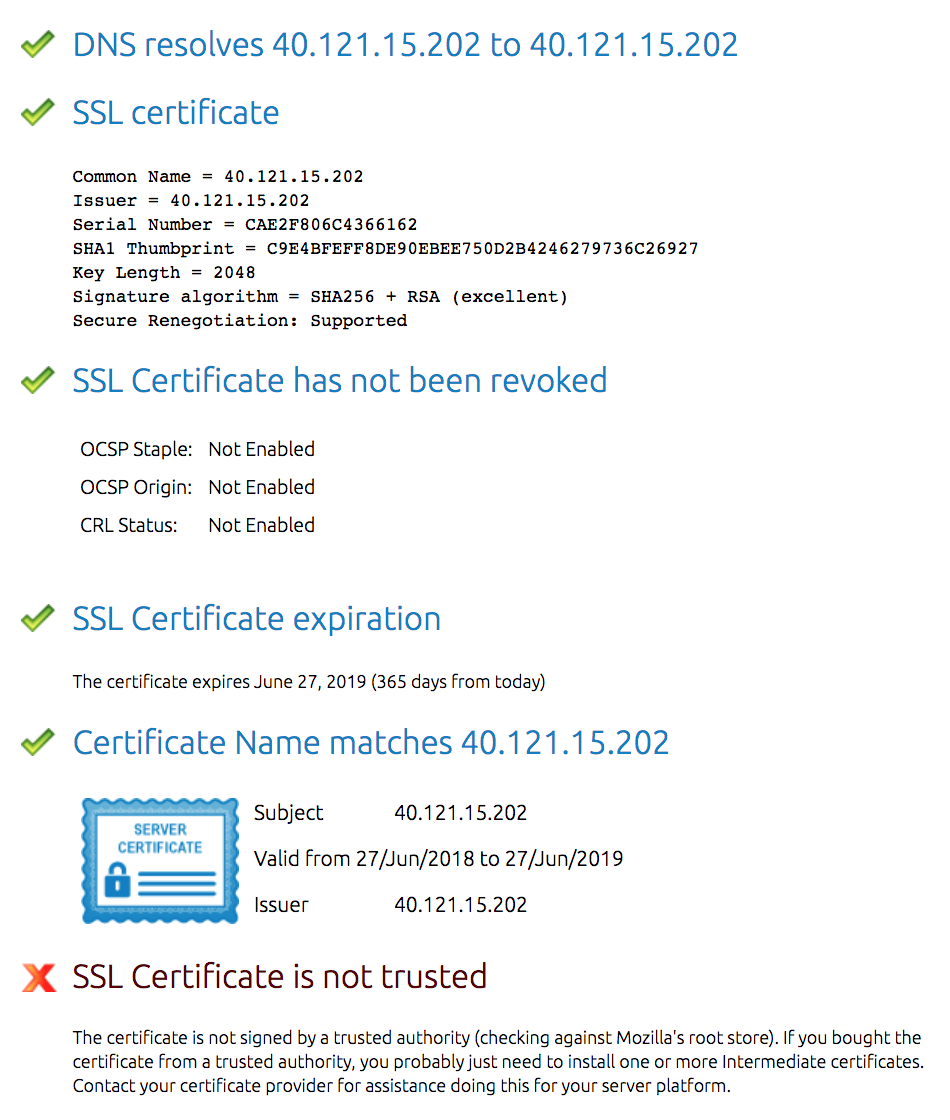
\includegraphics[width=10cm,height=10.9cm]{Images/implement/digicert} \\
				\label{fig:digicert} 
				\textbf{Fuente de comprobación:} \url{https://www.digicert.com/help/}
			\end{center}  
		\end{figure}	
			
		\begin{figure}[!ht]   
			\caption{Análisis de seguridad del certificado - Algoritmo de firma \gls{sha-a}-1.} 
			\begin{center} 
	 			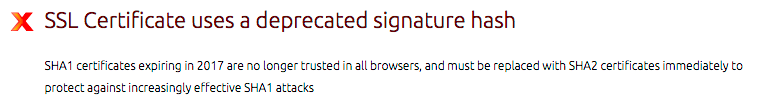
\includegraphics[width=16cm,height=1.5cm]{Images/implement/digicert_sha1} \\
				\label{fig:digicert_sha1} 
				\textbf{Fuente de comprobación:} \url{https://www.digicert.com/help/}
			\end{center}  
		\end{figure}	

	Las Figuras \ref{fig:comodo}, \ref{fig:htbridge1} y \ref{fig:htbridge2} muestran más información sobre el análisis realizado por otras herramientas poniendo énfasis en la configuración de seguridad. Algunos datos informativos obtenidos son: 
	
	\begin{itemize}
		\item El servidor presenta una buena configuración de seguridad con una calificación final de A- gracias al uso de las buenas prácticas recomendadas por la empresa Qualys SSL Labs\footnote{Para obtener más información sobre estas prácticas puede consultar la referencia \cite{ssllabs:best}.}.
		\item Solamente se admiten conexiones a través del protocolo \gls{tls-a} (\textit{\gls{tls}}). Esta configuración es la idónea puesto que el protocolo \gls{ssl-a} se considera inseguro debido a la gran cantidad de vulnerabilidades existentes: DROWN, FREAK, POODLE, etc.
		\item Se mitigan también otro tipo de vulnerabilidades: CRIME, Heartbleed, SLOTH, Robot, CVE-2014-0224 (OpenSSL CCS flaw), CVE-2016-2107 (OpenSSL padding-oracle flaw), etc.
		\item Solamente se permite la renegociación segura de los detalles de la comunicación. La renegociación insegura iniciada por el client no es soportada.
	\end{itemize}
					
	\begin{figure}[!ht]   
		\caption{Análisis de seguridad con High-Tech Bridge - Resumen.} 
		
		\begin{center} 
 			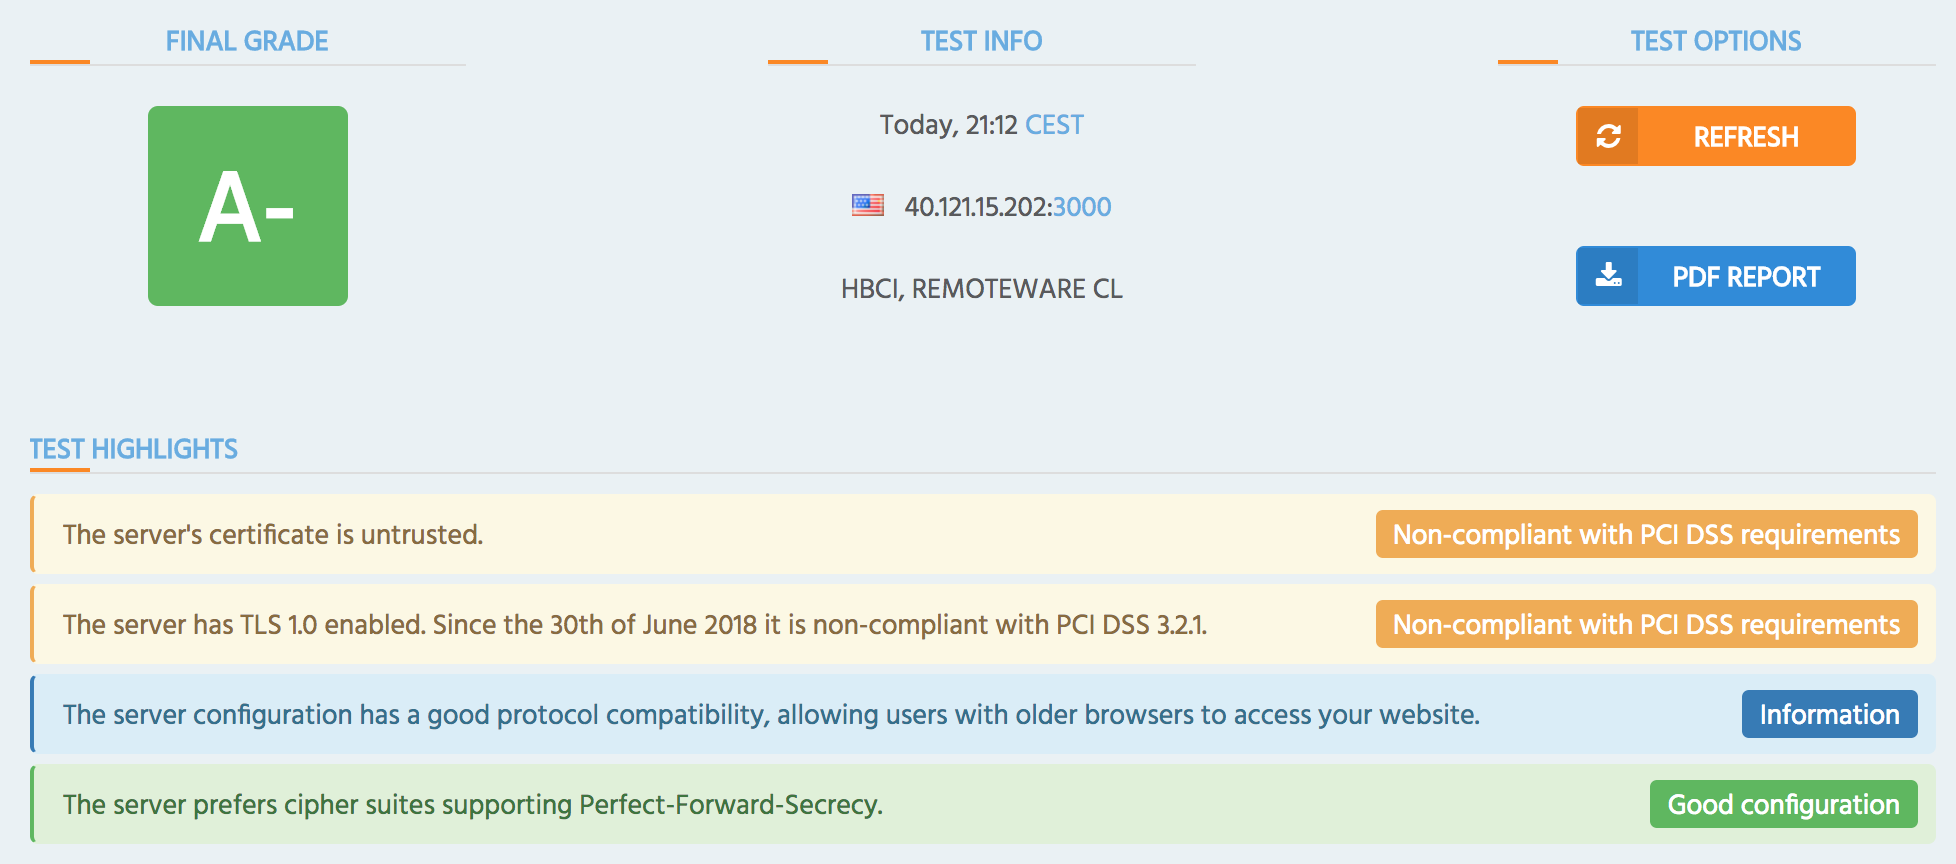
\includegraphics[width=15cm,height=5.5cm]{Images/implement/htbridge1} \\
			\label{fig:htbridge1} 
			\textbf{Fuente de comprobación:} \url{https://www.htbridge.com/ssl/}
		\end{center}  
	\end{figure}	
		
	\begin{figure}[!ht]   
		\caption{Análisis de seguridad con High-Tech Bridge - Vulnerabilidades no soportadas.} 
		\begin{center} 
	 		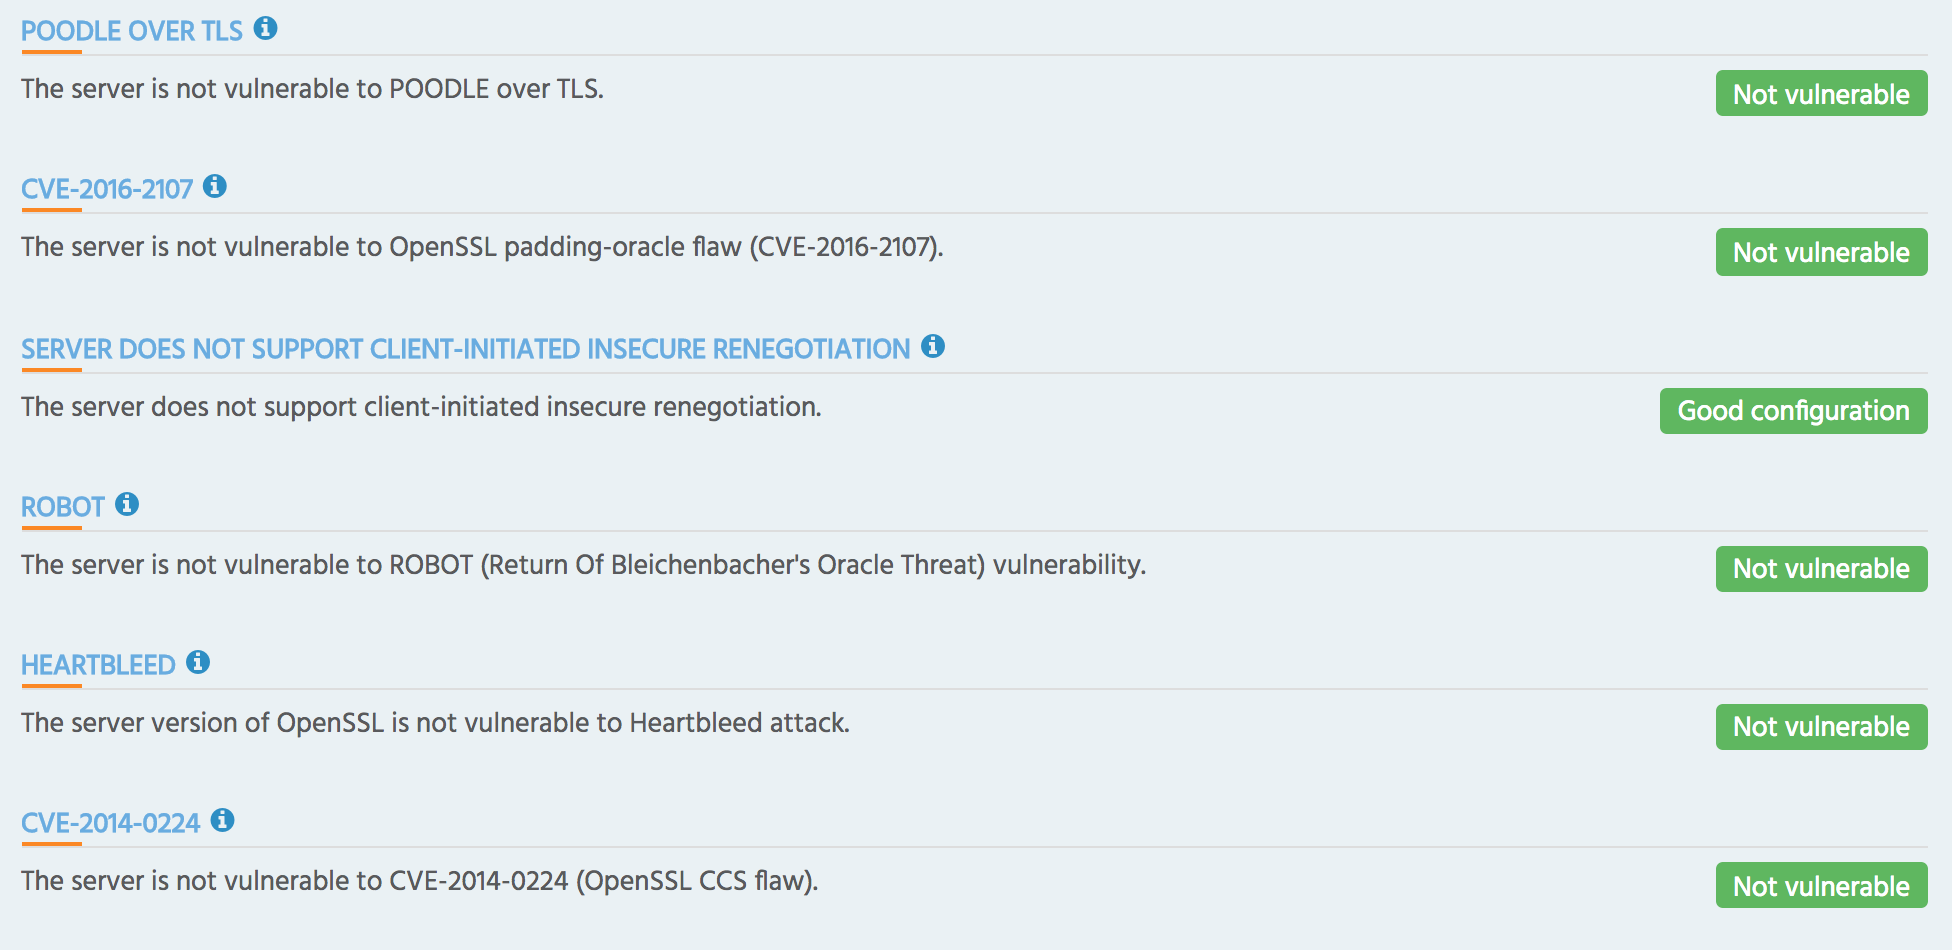
\includegraphics[width=15cm,height=5.5cm]{Images/implement/htbridge2} \\
			\label{fig:htbridge2} 
			\textbf{Fuente de comprobación:} \url{https://www.htbridge.com/ssl/}
		\end{center}  
	\end{figure}	
	
	\begin{figure}[!ht]   
		\caption{Análisis de seguridad con COMODO SSL Analyzer.} 
		\begin{center} 
			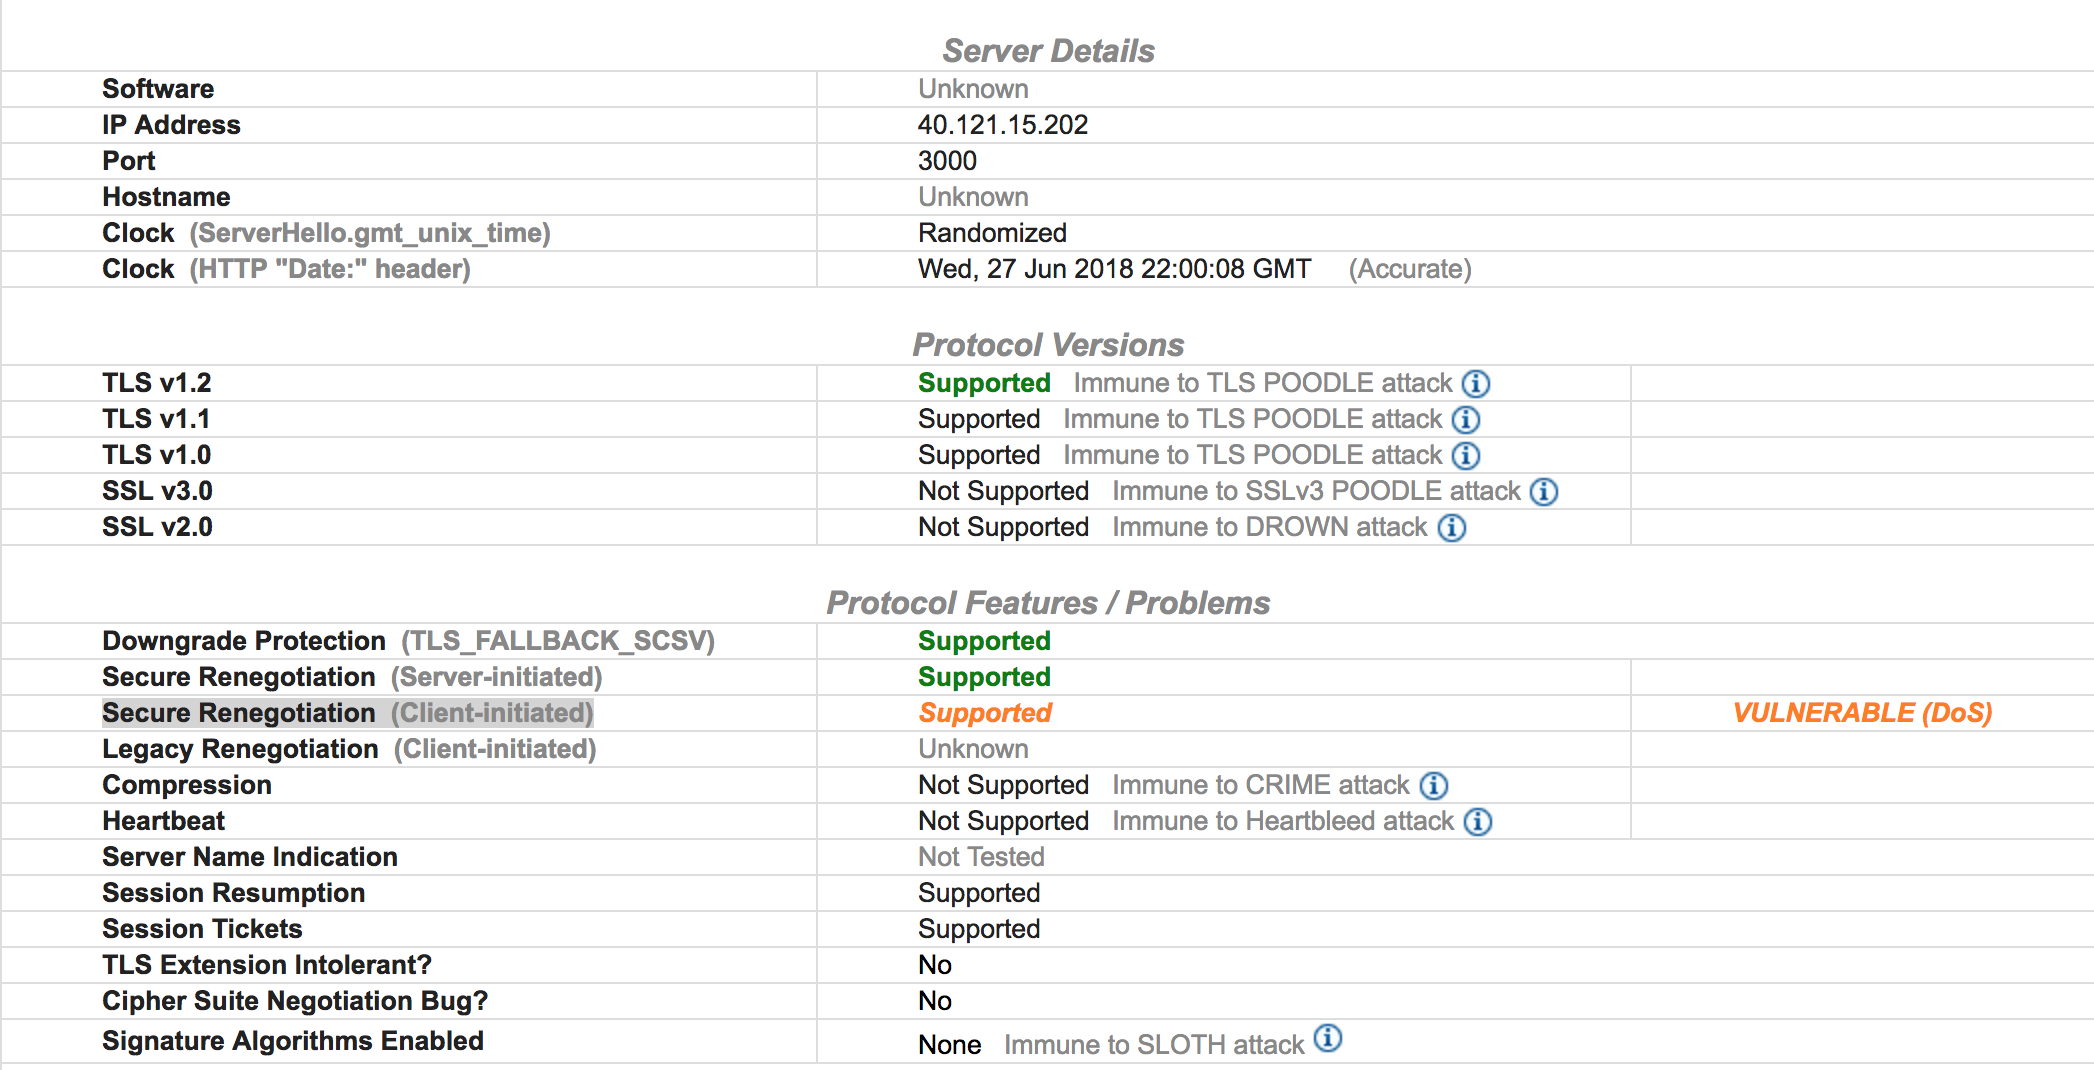
\includegraphics[width=16cm,height=10cm]{Images/implement/comodo} \\
			\label{fig:comodo} 
			\textbf{Fuente de comprobación:} \url{https://sslanalyzer.comodoca.com/}
		\end{center}  
	\end{figure}	
		
	Por último, se muestra un ejemplo de la configuración negociada entre el cliente y el servidor para el navegador Google Chrome v67.0.3396.99 (Figura \ref{fig:handshake}). \\ 
		
	\begin{figure}[!ht]   
		\caption{Configuración negociada en el navegador Google Chrome.} 
		\begin{center} 
			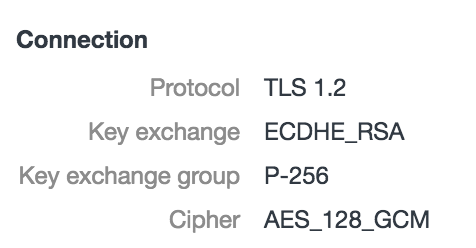
\includegraphics[width=6cm,height=2cm]{Images/implement/handshake} \\
			\label{fig:handshake} 
		\end{center}  
	\end{figure}	
					
	% Test cases
	\chapter{Casos de prueba} \label{testingChapter}
	
	\textbf{Resumen:} \textit{Toda implementación software requiere de varias fases de pruebas previas a la liberación de la versión de producción con el fin de garantizar la calidad en términos funcionales, de diseño, de seguridad, de rendimiento, etc. La información obtenida de este proceso es de vital importancia debido a que brinda la posibilidad de una detección temprana de errores e implicará en gran medida en el éxito o no del proyecto.}
	
	% Section
	\section{Introducción a los casos de prueba}
	
	Las pruebas o \textit{testing} son un conjunto de prácticas ubicadas en el proceso de control de calidad que se definen como el procedimiento de investigación y análisis de la calidad del \textit{software} con el fin principal de detectar errores de forma temprana y de proveer información útil a todos los interesados del proyecto o \textit{\glspl{stakeholder}}. Dentro del conjunto de pruebas, éstas se pueden diferenciar en función de los aspectos a ser probados:
	
	\begin{itemize}
		\item Funcionalidad, donde se prueba que el sistema funcione como se espera y para lo que fue diseñado. Ejemplo de pruebas de esta categoría: pruebas unitarias, de integración, de regresión, de aceptación, etc.
		\item Rendimiento, donde se localizan las pruebas de carga y de estrés cuyo objetivo es conocer el comportamiento del sistema ante diferentes situaciones de saturación y el punto donde el sistema deja de funcionar correctamente.
		\item Usabilidad y adaptabilidad para conocer si el sistema es intuitivo, fácil de usar y se adapta a diferentes entornos y tipos de personas. Ejemplo de pruebas de esta categoría: pruebas moderadas, \textit{card sorting}, pruebas A/B, evaluaciones heurísticas, etc.
		\item Seguridad para evaluar cómo de seguro es el sistema ante amenazas externas y para detectar vulnerabilidades. Ejemplo de pruebas de esta categoría: pruebas de penetración (\textit{pentesting}).
	\end{itemize}
	
	El marco temporal donde se debe ejecutar un determinado tipo de prueba varía en función de sus objetivos. Algunos se pueden aplicar desde fases tempranas del desarrollo como es el caso de las pruebas unitarias -verifican el correcto funcionamiento de los componentes del sistema- o las pruebas de integración -verifican la correcta interacción entre los distintos componentes- mientras que otros requieren de un producto mínimo viable (\textit{\gls{mvp}} -\gls{mvp-a}-) para poder obtener una retroalimentación como el caso de las pruebas \textit{End-to-End}, pruebas automatizadas del flujo completo del sistema que simulan al usuario final en un escenario de producción interactuando con la interfaz de usuario (\textit{\gls{ui}} -\gls{ui-a}-). \\

	En Hyot, durante la fase de construcción y transición a medida que se iba implementando la funcionalidad se han ido ejecutando pruebas unitarias para verificar el correcto funcionamiento de cada caso de uso involucrado en cada iteración y pruebas de integración para constatar la interacción entre las diferentes partes que componen este proyecto con el fin de garantizar la calidad del sistema y cumplir con los requisitos tanto funcionales como no funcionales que se han ido marcando en cada iteración. \\
	
	% Section
	\section{Casos de prueba}
	
	En esta sección se detallan los casos de prueba\footnote{Únicamente se plasman aquellos casos de prueba considerados de mayor importancia para no dilatar demasiado el documento. En algunos casos, el caso de prueba -marcado con el símbolo \textbf{\color{black!40!blue}*}- puede aplicar a varios componentes aunque puede diferir la salida exacta mostrada.} identificados y a los que se ha sometido cada componente del proyecto Hyot, así como los resultados de los mismos. Para describir cada caso de prueba se ha utilizado el siguiente esquema:
	
	\begin{itemize}
		\item \textbf{Caso de prueba:} identificador del caso de prueba.
		\item \textbf{Descripción:} descripción de la funcionalidad a probar.
		\item \textbf{Salida esperada:} resultado esperado tras la finalización de la prueba.
		\item \textbf{Salida obtenida:} resultado obtenido tras la finalización de la prueba.
		\item \textbf{Resultado de la prueba:} resultado final de la prueba.
	\end{itemize}
	
	% Subsection
	\subsection{Componente - Configuración del dispositivo Raspberry Pi}
	
	Los casos de prueba a continuación descritos hacen referencia al componente del proyecto Hyot que permite la configuración inicial del dispositivo \gls{raspberry} (\gls{raspberry-a})\footnote{Aquellos casos de prueba marcados con el símbolo \textbf{\color{black!40!blue}**} hacen referencia a la instalación de dependencias donde solamente se especificarán los referidos a paquetes, omitiendo aquellos referidos a librerías \gls{python} por su similitud.}.
	
	% New page
	\newpage
	
	% CP-0001: Ejecución sin el fichero de utilidades utils.sh
	\begin{longtable}{|p{3cm}|p{13cm}|}
		\hline
		
		\multicolumn{1}{|>{\columncolor{Gainsboro}}p{3.5cm}|}{\textsc{Caso de prueba}} & \multicolumn{1}{|>{\columncolor{Gainsboro}}c|}{\textsc{UC-0001}}
		\\ \hline
		\multicolumn{1}{|p{3.5cm}|}{Descripción} & \multicolumn{1}{p{13cm}|}{\textbf{Ejecución sin el fichero de utilidades utils.sh}} \\ \hline
		\multicolumn{1}{|p{3.5cm}|}{Salida esperada} & \multicolumn{1}{p{13cm}|}{Mensaje informativo y finalización de la ejecución} \\ \hline
		\multicolumn{1}{|p{3.5cm}|}{Salida obtenida} & \multicolumn{1}{p{13cm}|}{Mensaje informativo y finalización de la ejecución debido a la no localización del fichero} \\ \hline
		\multicolumn{1}{|p{3.5cm}|}{Estado} & \multicolumn{1}{p{13cm}|}{Finalizado} \\ \hline
		\multicolumn{1}{|p{3.5cm}|}{Resultado} & \multicolumn{1}{|>{\columncolor{dartmouthgreen!40}}p{13cm}|}{\textbf{Correcto}} \\ \hline
							
		\caption{Caso de prueba - Ejecución sin el fichero de utilidades utils.sh}
	\end{longtable}
	
	% CP-0002: Ejecución con usuario normal: pi
	\begin{longtable}{|p{3cm}|p{13cm}|}
		\hline
		
		\multicolumn{1}{|>{\columncolor{Gainsboro}}p{3.5cm}|}{\textsc{Caso de prueba}} & \multicolumn{1}{|>{\columncolor{Gainsboro}}c|}{\textsc{UC-0002}}
		\\ \hline
		\multicolumn{1}{|p{3.5cm}|}{Descripción} & \multicolumn{1}{p{13cm}|}{\textbf{Ejecución con usuario normal: pi \textbf{\color{black!40!blue}*}}} \\ \hline
		\multicolumn{1}{|p{3.5cm}|}{Salida esperada} & \multicolumn{1}{p{13cm}|}{Mensaje informativo: ``\textit{This component must be run as root}'' y finalización de la ejecución} \\ \hline
		\multicolumn{1}{|p{3.5cm}|}{Salida obtenida} & \multicolumn{1}{p{13cm}|}{Mensaje informativo y finalización de la ejecución debido a que el usuario no es un usuario superprivilegiado} \\ \hline
		\multicolumn{1}{|p{3.5cm}|}{Estado} & \multicolumn{1}{p{13cm}|}{Finalizado} \\ \hline
		\multicolumn{1}{|p{3.5cm}|}{Resultado} & \multicolumn{1}{|>{\columncolor{dartmouthgreen!40}}p{13cm}|}{\textbf{Correcto}} \\ \hline
									
		\caption{Caso de prueba - Ejecución con usuario normal: pi}
	\end{longtable}
	
	% CP-0003: Ejecución con sudo y usuario normal: pi
	\begin{longtable}{|p{3cm}|p{13cm}|}
		\hline
		
		\multicolumn{1}{|>{\columncolor{Gainsboro}}p{3.5cm}|}{\textsc{Caso de prueba}} & \multicolumn{1}{|>{\columncolor{Gainsboro}}c|}{\textsc{UC-0003}}
		\\ \hline
		\multicolumn{1}{|p{3.5cm}|}{Descripción} & \multicolumn{1}{p{13cm}|}{\textbf{Ejecución con sudo y usuario normal: pi \textbf{\color{black!40!blue}*}}} \\ \hline
		\multicolumn{1}{|p{3.5cm}|}{Salida esperada} & \multicolumn{1}{p{13cm}|}{Continuación de la ejecución} \\ \hline
		\multicolumn{1}{|p{3.5cm}|}{Salida obtenida} & \multicolumn{1}{p{13cm}|}{Comprobación de usuario correcta y continuación de la ejecución} \\ \hline
		\multicolumn{1}{|p{3.5cm}|}{Estado} & \multicolumn{1}{p{13cm}|}{Finalizado} \\ \hline
		\multicolumn{1}{|p{3.5cm}|}{Resultado} & \multicolumn{1}{|>{\columncolor{dartmouthgreen!40}}p{13cm}|}{\textbf{Correcto}} \\ \hline
								
		\caption{Caso de prueba - Ejecución con sudo y usuario normal: pi}
	\end{longtable}
	
	% CP-0004: Ejecución con usuario superprivilegiado: root
	\begin{longtable}{|p{3cm}|p{13cm}|}
		\hline
		
		\multicolumn{1}{|>{\columncolor{Gainsboro}}p{3.5cm}|}{\textsc{Caso de prueba}} & \multicolumn{1}{|>{\columncolor{Gainsboro}}c|}{\textsc{UC-0004}}
		\\ \hline
		\multicolumn{1}{|p{3.5cm}|}{Descripción} & \multicolumn{1}{p{13cm}|}{\textbf{Ejecución con usuario superprivilegiado: root \textbf{\color{black!40!blue}*}}} \\ \hline
		\multicolumn{1}{|p{3.5cm}|}{Salida esperada} & \multicolumn{1}{p{13cm}|}{Continuación de la ejecución} \\ \hline
		\multicolumn{1}{|p{3.5cm}|}{Salida obtenida} & \multicolumn{1}{p{13cm}|}{Comprobación de usuario correcta y continuación de la ejecución} \\ \hline
		\multicolumn{1}{|p{3.5cm}|}{Estado} & \multicolumn{1}{p{13cm}|}{Finalizado} \\ \hline
		\multicolumn{1}{|p{3.5cm}|}{Resultado} & \multicolumn{1}{|>{\columncolor{dartmouthgreen!40}}p{13cm}|}{\textbf{Correcto}} \\ \hline
							
		\caption{Caso de prueba - Ejecución con usuario superprivilegiado: root}
	\end{longtable}
	
	% CP-0005: Ejecución en el sistema operativo (SO): Windows 10
	\begin{longtable}{|p{3cm}|p{13cm}|}
		\hline
		
		\multicolumn{1}{|>{\columncolor{Gainsboro}}p{3.5cm}|}{\textsc{Caso de prueba}} & \multicolumn{1}{|>{\columncolor{Gainsboro}}c|}{\textsc{UC-0005}}
		\\ \hline
		\multicolumn{1}{|p{3.5cm}|}{Descripción} & \multicolumn{1}{p{13cm}|}{\textbf{Ejecución en el \gls{so} (\gls{so-a}): Windows 10 \textbf{\color{black!40!blue}*}}} \\ \hline
		\multicolumn{1}{|p{3.5cm}|}{Salida esperada} & \multicolumn{1}{p{13cm}|}{Mensaje informativo: ``\textit{This component must be run on GNU/Linux platform (e.g. Raspbian)}'' y finalización de la ejecución} \\ \hline
		\multicolumn{1}{|p{3.5cm}|}{Salida obtenida} & \multicolumn{1}{p{13cm}|}{Mensaje informativo y finalización de la ejecución al ser una plataforma no permitida} \\ \hline
		\multicolumn{1}{|p{3.5cm}|}{Estado} & \multicolumn{1}{p{13cm}|}{Finalizado} \\ \hline
		\multicolumn{1}{|p{3.5cm}|}{Resultado} & \multicolumn{1}{|>{\columncolor{dartmouthgreen!40}}p{13cm}|}{\textbf{Correcto}} \\ \hline
									
		\caption{Caso de prueba - Ejecución en el sistema operativo (SO): Windows 10}
	\end{longtable}
	
	% CP-0006: Ejecución en el SO: Ma0cOS High Sierra
	\begin{longtable}{|p{3cm}|p{13cm}|}
		\hline
		
		\multicolumn{1}{|>{\columncolor{Gainsboro}}p{3.5cm}|}{\textsc{Caso de prueba}} & \multicolumn{1}{|>{\columncolor{Gainsboro}}c|}{\textsc{UC-0006}}
		\\ \hline
		\multicolumn{1}{|p{3.5cm}|}{Descripción} & \multicolumn{1}{p{13cm}|}{\textbf{Ejecución en el \gls{so-a}: \gls{macos-a} (\textit{\gls{macos}}) High Sierra \textbf{\color{black!40!blue}*}}} \\ \hline
		\multicolumn{1}{|p{3.5cm}|}{Salida esperada} & \multicolumn{1}{p{13cm}|}{Mensaje informativo: ``\textit{This component must be run on GNU/Linux platform (e.g. Raspbian)}'' y finalización de la ejecución} \\ \hline
		\multicolumn{1}{|p{3.5cm}|}{Salida obtenida} & \multicolumn{1}{p{13cm}|}{Mensaje informativo y finalización de la ejecución al ser una plataforma no permitida} \\ \hline
		\multicolumn{1}{|p{3.5cm}|}{Estado} & \multicolumn{1}{p{13cm}|}{Finalizado} \\ \hline
		\multicolumn{1}{|p{3.5cm}|}{Resultado} & \multicolumn{1}{|>{\columncolor{dartmouthgreen!40}}p{13cm}|}{\textbf{Correcto}} \\ \hline
							
		\caption{Caso de prueba - Ejecución en el SO: MacOS High Sierra}
	\end{longtable}
	
	% CP-0007: Ejecución en el SO: Ubuntu
	\begin{longtable}{|p{3cm}|p{13cm}|}
		\hline
		
		\multicolumn{1}{|>{\columncolor{Gainsboro}}p{3.5cm}|}{\textsc{Caso de prueba}} & \multicolumn{1}{|>{\columncolor{Gainsboro}}c|}{\textsc{UC-0007}}
		\\ \hline
		\multicolumn{1}{|p{3.5cm}|}{Descripción} & \multicolumn{1}{p{13cm}|}{\textbf{Ejecución en el \gls{so-a}: Ubuntu \textbf{\color{black!40!blue}*}}} \\ \hline
		\multicolumn{1}{|p{3.5cm}|}{Salida esperada} & \multicolumn{1}{p{13cm}|}{Mensaje informativo: ``\textit{This component must be run on a Raspberry Pi}'' y finalización de la ejecución} \\ \hline
		\multicolumn{1}{|p{3.5cm}|}{Salida obtenida} & \multicolumn{1}{p{13cm}|}{Mensaje informativo y finalización de la ejecución al ser una plataforma \gls{gnulinux} no permitida} \\ \hline
		\multicolumn{1}{|p{3.5cm}|}{Estado} & \multicolumn{1}{p{13cm}|}{Finalizado} \\ \hline
		\multicolumn{1}{|p{3.5cm}|}{Resultado} & \multicolumn{1}{|>{\columncolor{dartmouthgreen!40}}p{13cm}|}{\textbf{Correcto}} \\ \hline
									
		\caption{Caso de prueba - Ejecución en el SO: Ubuntu}
	\end{longtable}
	
	% New page
	\newpage
	
	% CP-0008: Ejecución en el SBC: Arduino
	\begin{longtable}{|p{3cm}|p{13cm}|}
		\hline
		
		\multicolumn{1}{|>{\columncolor{Gainsboro}}p{3.5cm}|}{\textsc{Caso de prueba}} & \multicolumn{1}{|>{\columncolor{Gainsboro}}c|}{\textsc{UC-0008}}
		\\ \hline
		\multicolumn{1}{|p{3.5cm}|}{Descripción} & \multicolumn{1}{p{13cm}|}{\textbf{Ejecución en el \gls{sbc-a} (\textit{\gls{sbc}}): Arduino \textbf{\color{black!40!blue}*}}} \\ \hline
		\multicolumn{1}{|p{3.5cm}|}{Salida esperada} & \multicolumn{1}{p{13cm}|}{Mensaje informativo: ``\textit{This component must be run on a Raspberry Pi}'' y finalización de la ejecución} \\ \hline
		\multicolumn{1}{|p{3.5cm}|}{Salida obtenida} & \multicolumn{1}{p{13cm}|}{Mensaje informativo y finalización de la ejecución al ser un dispositivo no permitido} \\ \hline
		\multicolumn{1}{|p{3.5cm}|}{Estado} & \multicolumn{1}{p{13cm}|}{Finalizado} \\ \hline
		\multicolumn{1}{|p{3.5cm}|}{Resultado} & \multicolumn{1}{|>{\columncolor{dartmouthgreen!40}}p{13cm}|}{\textbf{Correcto}} \\ \hline
							
		\caption{Caso de prueba - Ejecución en el SBC (Single Board Computer): Arduino}
	\end{longtable}
	
	% CP-0009: Ejecución en el SBC: Raspberry Pi 2
	\begin{longtable}{|p{3cm}|p{13cm}|}
		\hline
		
		\multicolumn{1}{|>{\columncolor{Gainsboro}}p{3.5cm}|}{\textsc{Caso de prueba}} & \multicolumn{1}{|>{\columncolor{Gainsboro}}c|}{\textsc{UC-0009}}
		\\ \hline
		\multicolumn{1}{|p{3.5cm}|}{Descripción} & \multicolumn{1}{p{13cm}|}{\textbf{Ejecución en el \gls{sbc-a}: \gls{raspberry-a} 2 \textbf{\color{black!40!blue}*}}} \\ \hline
		\multicolumn{1}{|p{3.5cm}|}{Salida esperada} & \multicolumn{1}{p{13cm}|}{Continuación de la ejecución} \\ \hline
		\multicolumn{1}{|p{3.5cm}|}{Salida obtenida} & \multicolumn{1}{p{13cm}|}{Comprobación de plataforma y dispositivo correcta. Continuación de la ejecución} \\ \hline
		\multicolumn{1}{|p{3.5cm}|}{Estado} & \multicolumn{1}{p{13cm}|}{Finalizado} \\ \hline
		\multicolumn{1}{|p{3.5cm}|}{Resultado} & \multicolumn{1}{|>{\columncolor{dartmouthgreen!40}}p{13cm}|}{\textbf{Correcto}} \\ \hline
							
		\caption{Caso de prueba - Ejecución en el SBC: RPi 2}
	\end{longtable}
	
	% CP-0010: Ejecución sin el comando wget instalado
	\begin{longtable}{|p{3cm}|p{13cm}|}
		\hline
		
		\multicolumn{1}{|>{\columncolor{Gainsboro}}p{3.5cm}|}{\textsc{Caso de prueba}} & \multicolumn{1}{|>{\columncolor{Gainsboro}}c|}{\textsc{UC-0010}}
		\\ \hline
		\multicolumn{1}{|p{3.5cm}|}{Descripción} & \multicolumn{1}{p{13cm}|}{\textbf{Ejecución sin el comando wget instalado}} \\ \hline
		\multicolumn{1}{|p{3.5cm}|}{Salida esperada} & \multicolumn{1}{p{13cm}|}{Mensaje informativo: ``\textit{Command not found: wget. Please, install this command to check if the network connection is available}'' y finalización de la ejecución} \\ \hline
		\multicolumn{1}{|p{3.5cm}|}{Salida obtenida} & \multicolumn{1}{p{13cm}|}{Mensaje informativo y finalización de la ejecución debido a que el comando no se encuentra instalado en la \gls{raspberry-a}} \\ \hline
		\multicolumn{1}{|p{3.5cm}|}{Estado} & \multicolumn{1}{p{13cm}|}{Finalizado} \\ \hline
		\multicolumn{1}{|p{3.5cm}|}{Resultado} & \multicolumn{1}{|>{\columncolor{dartmouthgreen!40}}p{13cm}|}{\textbf{Correcto}} \\ \hline
									
		\caption{Caso de prueba - Ejecución sin el comando wget instalado}
	\end{longtable}
	
	% New page
	\newpage
	
	% CP-0011: Ejecución sin conexión a Internet
	\begin{longtable}{|p{3cm}|p{13cm}|}
		\hline
		
		\multicolumn{1}{|>{\columncolor{Gainsboro}}p{3.5cm}|}{\textsc{Caso de prueba}} & \multicolumn{1}{|>{\columncolor{Gainsboro}}c|}{\textsc{UC-0011}}
		\\ \hline
		\multicolumn{1}{|p{3.5cm}|}{Descripción} & \multicolumn{1}{p{13cm}|}{\textbf{Ejecución sin conexión a Internet \textbf{\color{black!40!blue}*}}} \\ \hline
		\multicolumn{1}{|p{3.5cm}|}{Salida esperada} & \multicolumn{1}{p{13cm}|}{Mensaje informativo: ``\textit{Raspberry Pi is not connected to the network. Please, enable the network to continue the setup}'' y finalización de la ejecución} \\ \hline
		\multicolumn{1}{|p{3.5cm}|}{Salida obtenida} & \multicolumn{1}{p{13cm}|}{Mensaje informativo y finalización de la ejecución debido a que la \gls{raspberry-a} no posee red} \\ \hline
		\multicolumn{1}{|p{3.5cm}|}{Estado} & \multicolumn{1}{p{13cm}|}{Finalizado} \\ \hline
		\multicolumn{1}{|p{3.5cm}|}{Resultado} & \multicolumn{1}{|>{\columncolor{dartmouthgreen!40}}p{13cm}|}{\textbf{Correcto}} \\ \hline
							
		\caption{Caso de prueba - Ejecución sin conexión a Internet}
	\end{longtable}
	
	% CP-0012: Ejecución sin el comando pgrep instalado
	\begin{longtable}{|p{3cm}|p{13cm}|}
		\hline
		
		\multicolumn{1}{|>{\columncolor{Gainsboro}}p{3.5cm}|}{\textsc{Caso de prueba}} & \multicolumn{1}{|>{\columncolor{Gainsboro}}c|}{\textsc{UC-0012}}
		\\ \hline
		\multicolumn{1}{|p{3.5cm}|}{Descripción} & \multicolumn{1}{p{13cm}|}{\textbf{Ejecución sin el comando pgrep instalado}} \\ \hline
		\multicolumn{1}{|p{3.5cm}|}{Salida esperada} & \multicolumn{1}{p{13cm}|}{Mensaje informativo: ``\textit{Command not found: pgrep. Please, install this command to check and avoid the concurrency}'' y finalización de la ejecución} \\ \hline
		\multicolumn{1}{|p{3.5cm}|}{Salida obtenida} & \multicolumn{1}{p{13cm}|}{Mensaje informativo y finalización de la ejecución debido a que el comando no se encuentra instalado en la \gls{raspberry-a}} \\ \hline
		\multicolumn{1}{|p{3.5cm}|}{Estado} & \multicolumn{1}{p{13cm}|}{Finalizado} \\ \hline
		\multicolumn{1}{|p{3.5cm}|}{Resultado} & \multicolumn{1}{|>{\columncolor{dartmouthgreen!40}}p{13cm}|}{\textbf{Correcto}} \\ \hline
							
		\caption{Caso de prueba - Ejecución sin el comando pgrep instalado}
	\end{longtable}
	
	% CP-0013: Ejecución cuando otra instancia ya está ejecutándose
	\begin{longtable}{|p{3cm}|p{13cm}|}
		\hline
		
		\multicolumn{1}{|>{\columncolor{Gainsboro}}p{3.5cm}|}{\textsc{Caso de prueba}} & \multicolumn{1}{|>{\columncolor{Gainsboro}}c|}{\textsc{UC-0013}}
		\\ \hline
		\multicolumn{1}{|p{3.5cm}|}{Descripción} & \multicolumn{1}{p{13cm}|}{\textbf{Ejecución cuando otra instancia ya está ejecutándose \textbf{\color{black!40!blue}*}}} \\ \hline
		\multicolumn{1}{|p{3.5cm}|}{Salida esperada} & \multicolumn{1}{p{13cm}|}{Mensaje informativo: ``\textit{Process: raspberrypi\_setup.sh is already running with PID [pid]}'' y finalización de la ejecución} \\ \hline
		\multicolumn{1}{|p{3.5cm}|}{Salida obtenida} & \multicolumn{1}{p{13cm}|}{Mensaje informativo y finalización de la ejecución debido a que otra instancia está en ejecución} \\ \hline
		\multicolumn{1}{|p{3.5cm}|}{Estado} & \multicolumn{1}{p{13cm}|}{Finalizado} \\ \hline
		\multicolumn{1}{|p{3.5cm}|}{Resultado} & \multicolumn{1}{|>{\columncolor{dartmouthgreen!40}}p{13cm}|}{\textbf{Correcto}} \\ \hline
							
		\caption{Caso de prueba - Ejecución cuando otra instancia ya está ejecutándose}
	\end{longtable}
	
	% New page
	\newpage
	
	% CP-0014: Ejecución con las opciones: -h, -v y -p
	\begin{longtable}{|p{3cm}|p{13cm}|}
		\hline
		
		\multicolumn{1}{|>{\columncolor{Gainsboro}}p{3.5cm}|}{\textsc{Caso de prueba}} & \multicolumn{1}{|>{\columncolor{Gainsboro}}c|}{\textsc{UC-0014}}
		\\ \hline
		\multicolumn{1}{|p{3.5cm}|}{Descripción} & \multicolumn{1}{p{13cm}|}{\textbf{Ejecución con las opciones: -h, -v y -p}} \\ \hline
		\multicolumn{1}{|p{3.5cm}|}{Salida esperada} & \multicolumn{1}{p{13cm}|}{Mensaje informativo: ``\textit{Invalid parameter number. Please, type the `-h' or `--help' option to show the help}'' y finalización de la ejecución} \\ \hline
		\multicolumn{1}{|p{3.5cm}|}{Salida obtenida} & \multicolumn{1}{p{13cm}|}{Mensaje informativo y finalización de la ejecución debido a que el número de opciones introducido es inválido} \\ \hline
		\multicolumn{1}{|p{3.5cm}|}{Estado} & \multicolumn{1}{p{13cm}|}{Finalizado} \\ \hline
		\multicolumn{1}{|p{3.5cm}|}{Resultado} & \multicolumn{1}{|>{\columncolor{dartmouthgreen!40}}p{13cm}|}{\textbf{Correcto}} \\ \hline
													
		\caption{Caso de prueba - Ejecución con las opciones: --h, -v y -p}
	\end{longtable}

	% CP-0015: Ejecución con la opción: -h o --help
	\begin{longtable}{|p{3cm}|p{13cm}|}
		\hline
		
		\multicolumn{1}{|>{\columncolor{Gainsboro}}p{3.5cm}|}{\textsc{Caso de prueba}} & \multicolumn{1}{|>{\columncolor{Gainsboro}}c|}{\textsc{UC-0015}}
		\\ \hline
		\multicolumn{1}{|p{3.5cm}|}{Descripción} & \multicolumn{1}{p{13cm}|}{\textbf{Ejecución con la opción: -h o --help \textbf{\color{black!40!blue}*}}} \\ \hline
		\multicolumn{1}{|p{3.5cm}|}{Salida esperada} & \multicolumn{1}{p{13cm}|}{Se muestra la ayuda} \\ \hline
		\multicolumn{1}{|p{3.5cm}|}{Salida obtenida} & \multicolumn{1}{p{13cm}|}{La ayuda es mostrada y la ejecución es finalizada posteriormente} \\ \hline
		\multicolumn{1}{|p{3.5cm}|}{Estado} & \multicolumn{1}{p{13cm}|}{Finalizado} \\ \hline
		\multicolumn{1}{|p{3.5cm}|}{Resultado} & \multicolumn{1}{|>{\columncolor{dartmouthgreen!40}}p{13cm}|}{\textbf{Correcto}} \\ \hline
									
		\caption{Caso de prueba - Ejecución con la opción: -h o --help}
	\end{longtable}
	
	% CP-0016: Ejecución con la opción: -v o --verbose
	\begin{longtable}{|p{3cm}|p{13cm}|}
		\hline
		
		\multicolumn{1}{|>{\columncolor{Gainsboro}}p{3.5cm}|}{\textsc{Caso de prueba}} & \multicolumn{1}{|>{\columncolor{Gainsboro}}c|}{\textsc{UC-0016}}
		\\ \hline
		\multicolumn{1}{|p{3.5cm}|}{Descripción} & \multicolumn{1}{p{13cm}|}{\textbf{Ejecución con la opción: -v o --verbose}} \\ \hline
		\multicolumn{1}{|p{3.5cm}|}{Salida esperada} & \multicolumn{1}{p{13cm}|}{Se activa el modo \textit{verbose}} \\ \hline
		\multicolumn{1}{|p{3.5cm}|}{Salida obtenida} & \multicolumn{1}{p{13cm}|}{La ejecución continúa y se muestra más información sobre ésta} \\ \hline
		\multicolumn{1}{|p{3.5cm}|}{Estado} & \multicolumn{1}{p{13cm}|}{Finalizado} \\ \hline
		\multicolumn{1}{|p{3.5cm}|}{Resultado} & \multicolumn{1}{|>{\columncolor{dartmouthgreen!40}}p{13cm}|}{\textbf{Correcto}} \\ \hline
							
		\caption{Caso de prueba - Ejecución con la opción: -v o --verbose}
	\end{longtable}
	
	% CP-0017: Ejecución con la opción: -p o --packages
	\begin{longtable}{|p{3cm}|p{13cm}|}
		\hline
		
		\multicolumn{1}{|>{\columncolor{Gainsboro}}p{3.5cm}|}{\textsc{Caso de prueba}} & \multicolumn{1}{|>{\columncolor{Gainsboro}}c|}{\textsc{UC-0017}}
		\\ \hline
		\multicolumn{1}{|p{3.5cm}|}{Descripción} & \multicolumn{1}{p{13cm}|}{\textbf{Ejecución con la opción: -p o --packages}} \\ \hline
		\multicolumn{1}{|p{3.5cm}|}{Salida esperada} & \multicolumn{1}{p{13cm}|}{Ejecuta solamente la instalación de paquetes y librerías \gls{python}} \\ \hline
		\multicolumn{1}{|p{3.5cm}|}{Salida obtenida} & \multicolumn{1}{p{13cm}|}{Instala y/o actualiza las dependencias} \\ \hline
		\multicolumn{1}{|p{3.5cm}|}{Estado} & \multicolumn{1}{p{13cm}|}{Finalizado} \\ \hline
		\multicolumn{1}{|p{3.5cm}|}{Resultado} & \multicolumn{1}{|>{\columncolor{dartmouthgreen!40}}p{13cm}|}{\textbf{Correcto}} \\ \hline
							
		\caption{Caso de prueba - Ejecución con la opción: -p o --packages}
	\end{longtable}
	
	% CP-0018: Ejecución con la opción: -i o --interfaces
	\begin{longtable}{|p{3cm}|p{13cm}|}
		\hline
		
		\multicolumn{1}{|>{\columncolor{Gainsboro}}p{3.5cm}|}{\textsc{Caso de prueba}} & \multicolumn{1}{|>{\columncolor{Gainsboro}}c|}{\textsc{UC-0018}}
		\\ \hline
		\multicolumn{1}{|p{3.5cm}|}{Descripción} & \multicolumn{1}{p{13cm}|}{\textbf{Ejecución con la opción: -i o --interfaces}} \\ \hline
		\multicolumn{1}{|p{3.5cm}|}{Salida esperada} & \multicolumn{1}{p{13cm}|}{Ejecuta solamente la activación de las interfaces} \\ \hline
		\multicolumn{1}{|p{3.5cm}|}{Salida obtenida} & \multicolumn{1}{p{13cm}|}{Habilita las interfaces} \\ \hline
		\multicolumn{1}{|p{3.5cm}|}{Estado} & \multicolumn{1}{p{13cm}|}{Finalizado} \\ \hline
		\multicolumn{1}{|p{3.5cm}|}{Resultado} & \multicolumn{1}{|>{\columncolor{dartmouthgreen!40}}p{13cm}|}{\textbf{Correcto}} \\ \hline
							
		\caption{Caso de prueba - Ejecución con la opción: -i o --interfaces}
	\end{longtable}
	
	% CP-0019: Ejecución con las opciones: -v y -p
	\begin{longtable}{|p{3cm}|p{13cm}|}
		\hline
		
		\multicolumn{1}{|>{\columncolor{Gainsboro}}p{3.5cm}|}{\textsc{Caso de prueba}} & \multicolumn{1}{|>{\columncolor{Gainsboro}}c|}{\textsc{UC-0019}}
		\\ \hline
		\multicolumn{1}{|p{3.5cm}|}{Descripción} & \multicolumn{1}{p{13cm}|}{\textbf{Ejecución con las opciones: -v y -p}} \\ \hline
		\multicolumn{1}{|p{3.5cm}|}{Salida esperada} & \multicolumn{1}{p{13cm}|}{Ejecuta solamente la instalación de paquetes y librerías \gls{python} activando el modo \textit{verbose}} \\ \hline
		\multicolumn{1}{|p{3.5cm}|}{Salida obtenida} & \multicolumn{1}{p{13cm}|}{Instala y/o actualiza las dependencias mostrando más información sobre el proceso} \\ \hline
		\multicolumn{1}{|p{3.5cm}|}{Estado} & \multicolumn{1}{p{13cm}|}{Finalizado} \\ \hline
		\multicolumn{1}{|p{3.5cm}|}{Resultado} & \multicolumn{1}{|>{\columncolor{dartmouthgreen!40}}p{13cm}|}{\textbf{Correcto}} \\ \hline
							
		\caption{Caso de prueba - Ejecución con las opciones: -v y -p}
	\end{longtable}
	
	% CP-0020: Ejecución con las opciones: -v y -i
	\begin{longtable}{|p{3cm}|p{13cm}|}
		\hline
		
		\multicolumn{1}{|>{\columncolor{Gainsboro}}p{3.5cm}|}{\textsc{Caso de prueba}} & \multicolumn{1}{|>{\columncolor{Gainsboro}}c|}{\textsc{UC-0020}}
		\\ \hline
		\multicolumn{1}{|p{3.5cm}|}{Descripción} & \multicolumn{1}{p{13cm}|}{\textbf{Ejecución con las opciones: -v y -i}} \\ \hline
		\multicolumn{1}{|p{3.5cm}|}{Salida esperada} & \multicolumn{1}{p{13cm}|}{Ejecuta solamente la activación de interfaces habilitando el modo \textit{verbose}} \\ \hline
		\multicolumn{1}{|p{3.5cm}|}{Salida obtenida} & \multicolumn{1}{p{13cm}|}{Habilita las interfaces mostrando más información sobre el proceso} \\ \hline
		\multicolumn{1}{|p{3.5cm}|}{Estado} & \multicolumn{1}{p{13cm}|}{Finalizado} \\ \hline
		\multicolumn{1}{|p{3.5cm}|}{Resultado} & \multicolumn{1}{|>{\columncolor{dartmouthgreen!40}}p{13cm}|}{\textbf{Correcto}} \\ \hline
							
		\caption{Caso de prueba - Ejecución con las opciones: -v y -i}
	\end{longtable}
	
	% CP-0021: Ejecución con una opción inválida (-a)
	\begin{longtable}{|p{3cm}|p{13cm}|}
		\hline
		
		\multicolumn{1}{|>{\columncolor{Gainsboro}}p{3.5cm}|}{\textsc{Caso de prueba}} & \multicolumn{1}{|>{\columncolor{Gainsboro}}c|}{\textsc{UC-0021}}
		\\ \hline
		\multicolumn{1}{|p{3.5cm}|}{Descripción} & \multicolumn{1}{p{13cm}|}{\textbf{Ejecución con una opción inválida (-a) \textbf{\color{black!40!blue}*}}} \\ \hline
		\multicolumn{1}{|p{3.5cm}|}{Salida esperada} & \multicolumn{1}{p{13cm}|}{Mensaje informativo: ``\textit{Unknown option: -a. Please, type the option `-h' or `--help' to show the help}'' y finalización  de la ejecución} \\ \hline
		\multicolumn{1}{|p{3.5cm}|}{Salida obtenida} & \multicolumn{1}{p{13cm}|}{Mensaje y finalización de la ejecución debido a una opción inválida} \\ \hline
		\multicolumn{1}{|p{3.5cm}|}{Estado} & \multicolumn{1}{p{13cm}|}{Finalizado} \\ \hline
		\multicolumn{1}{|p{3.5cm}|}{Resultado} & \multicolumn{1}{|>{\columncolor{dartmouthgreen!40}}p{13cm}|}{\textbf{Correcto}} \\ \hline
		
		\caption{Caso de prueba - Ejecución con una opción inválida (-a)}
	\end{longtable}
	
	% CP-0022: Ejecución sin los comandos apt-get, apt-cache y/o dpkg instalados
	\begin{longtable}{|p{3cm}|p{13cm}|}
		\hline
		
		\multicolumn{1}{|>{\columncolor{Gainsboro}}p{3.5cm}|}{\textsc{Caso de prueba}} & \multicolumn{1}{|>{\columncolor{Gainsboro}}c|}{\textsc{UC-0022}}
		\\ \hline
		\multicolumn{1}{|p{3.5cm}|}{Descripción} & \multicolumn{1}{p{13cm}|}{\textbf{Ejecución sin los comandos apt-get, apt-cache y/o dpkg instalados}} \\ \hline
		\multicolumn{1}{|p{3.5cm}|}{Salida esperada} & \multicolumn{1}{p{13cm}|}{Mensaje informativo: ``\textit{Command line tool: [command] is not installed in the system. Please, install this package before continuing}'' y finalización de la ejecución} \\ \hline
		\multicolumn{1}{|p{3.5cm}|}{Salida obtenida} & \multicolumn{1}{p{13cm}|}{Mensaje informativo y finalización de la ejecución debido a que alguno o todos los comandos no se encuentran instalados en la \gls{raspberry-a}} \\ \hline
		\multicolumn{1}{|p{3.5cm}|}{Estado} & \multicolumn{1}{p{13cm}|}{Finalizado} \\ \hline
		\multicolumn{1}{|p{3.5cm}|}{Resultado} & \multicolumn{1}{|>{\columncolor{dartmouthgreen!40}}p{13cm}|}{\textbf{Correcto}} \\ \hline
						
		\caption{Caso de prueba - Ejecución sin los comandos apt-get, apt-cache y/o dpkg instalados}
	\end{longtable}
	
	% CP-0023: Ejecución en un entorno sin el paquete python-pip instalado
	\begin{longtable}{|p{3cm}|p{13cm}|}
		\hline
		
		\multicolumn{1}{|>{\columncolor{Gainsboro}}p{3.5cm}|}{\textsc{Caso de prueba}} & \multicolumn{1}{|>{\columncolor{Gainsboro}}c|}{\textsc{UC-0023}}
		\\ \hline
		\multicolumn{1}{|p{3.5cm}|}{Descripción} & \multicolumn{1}{p{13cm}|}{\textbf{Ejecución en un entorno sin el paquete python-pip instalado \textbf{\color{black!40!blue}**}}} \\ \hline
		\multicolumn{1}{|p{3.5cm}|}{Salida esperada} & \multicolumn{1}{p{13cm}|}{Mensaje informativo: ``\textit{Package: python-pip was installed successfully}'' y continuación de la ejecución} \\ \hline
		\multicolumn{1}{|p{3.5cm}|}{Salida obtenida} & \multicolumn{1}{p{13cm}|}{Instalación del paquete y continuación de la ejecución} \\ \hline
		\multicolumn{1}{|p{3.5cm}|}{Estado} & \multicolumn{1}{p{13cm}|}{Finalizado} \\ \hline
		\multicolumn{1}{|p{3.5cm}|}{Resultado} & \multicolumn{1}{|>{\columncolor{dartmouthgreen!40}}p{13cm}|}{\textbf{Correcto}} \\ \hline
							
		\caption{Caso de prueba - Ejecución en un entorno sin el paquete python-pip instalado}
	\end{longtable}
	
	% CP-0024: Ejecución en un entorno sin el paquete python-pip instalado. Error de instalación
	\begin{longtable}{|p{3cm}|p{13cm}|}
		\hline
		
		\multicolumn{1}{|>{\columncolor{Gainsboro}}p{3.5cm}|}{\textsc{Caso de prueba}} & \multicolumn{1}{|>{\columncolor{Gainsboro}}c|}{\textsc{UC-0024}}
		\\ \hline
		\multicolumn{1}{|p{3.5cm}|}{Descripción} & \multicolumn{1}{p{13cm}|}{\textbf{Ejecución en un entorno sin el paquete python-pip instalado. Error de instalación \textbf{\color{black!40!blue}**}}} \\ \hline
		\multicolumn{1}{|p{3.5cm}|}{Salida esperada} & \multicolumn{1}{p{13cm}|}{Mensaje informativo: ``\textit{Error to install the package: python-pip}'' y finalización de la ejecución} \\ \hline
		\multicolumn{1}{|p{3.5cm}|}{Salida obtenida} & \multicolumn{1}{p{13cm}|}{Mensaje informativo y finalización de la ejecución debido a un error} \\ \hline
		\multicolumn{1}{|p{3.5cm}|}{Estado} & \multicolumn{1}{p{13cm}|}{Finalizado} \\ \hline
		\multicolumn{1}{|p{3.5cm}|}{Resultado} & \multicolumn{1}{|>{\columncolor{dartmouthgreen!40}}p{13cm}|}{\textbf{Correcto}} \\ \hline
									
		\caption{Caso de prueba - Ejecución en un entorno sin el paquete python-pip instalado. Error de instalación}
	\end{longtable}
	
	% New page
	\newpage
		
	% CP-0025: Ejecución en un entorno sin el paquete gnupg-nonexistent instalado
	\begin{longtable}{|p{3cm}|p{13cm}|}
		\hline
		
		\multicolumn{1}{|>{\columncolor{Gainsboro}}p{3.5cm}|}{\textsc{Caso de prueba}} & \multicolumn{1}{|>{\columncolor{Gainsboro}}c|}{\textsc{UC-0025}}
		\\ \hline
		\multicolumn{1}{|p{3.5cm}|}{Descripción} & \multicolumn{1}{p{13cm}|}{\textbf{Ejecución en un entorno sin el paquete gnupg-nonexistent instalado \textbf{\color{black!40!blue}**}}} \\ \hline
		\multicolumn{1}{|p{3.5cm}|}{Salida esperada} & \multicolumn{1}{p{13cm}|}{Mensaje informativo: ``\textit{Package: gnupg-nonexistent not found in the repository. Please, check its name}'' y finalización de la ejecución} \\ \hline
		\multicolumn{1}{|p{3.5cm}|}{Salida obtenida} & \multicolumn{1}{p{13cm}|}{Mensaje informativo y finalización de la ejecución debido a que el paquete no existe en el repositorio} \\ \hline
		\multicolumn{1}{|p{3.5cm}|}{Estado} & \multicolumn{1}{p{13cm}|}{Finalizado} \\ \hline
		\multicolumn{1}{|p{3.5cm}|}{Resultado} & \multicolumn{1}{|>{\columncolor{dartmouthgreen!40}}p{13cm}|}{\textbf{Correcto}} \\ \hline
			
		\caption{Caso de prueba - Ejecución en un entorno sin el paquete gnupg-nonexistent instalado}
	\end{longtable}
	
	% CP-0026: Ejecución en un entorno con el paquete i2c-tools instalado y actualizado
	\begin{longtable}{|p{3cm}|p{13cm}|}
		\hline
		
		\multicolumn{1}{|>{\columncolor{Gainsboro}}p{3.5cm}|}{\textsc{Caso de prueba}} & \multicolumn{1}{|>{\columncolor{Gainsboro}}c|}{\textsc{UC-0026}}
		\\ \hline
		\multicolumn{1}{|p{3.5cm}|}{Descripción} & \multicolumn{1}{p{13cm}|}{\textbf{Ejecución en un entorno con el paquete i2c-tools instalado y actualizado \textbf{\color{black!40!blue}**}}} \\ \hline
		\multicolumn{1}{|p{3.5cm}|}{Salida esperada} & \multicolumn{1}{p{13cm}|}{Mensaje informativo: ``\textit{Package is already updated to the last version}'' y continuación de la ejecución} \\ \hline
		\multicolumn{1}{|p{3.5cm}|}{Salida obtenida} & \multicolumn{1}{p{13cm}|}{Mensaje informativo y continuación de la ejecución} \\ \hline
		\multicolumn{1}{|p{3.5cm}|}{Estado} & \multicolumn{1}{p{13cm}|}{Finalizado} \\ \hline
		\multicolumn{1}{|p{3.5cm}|}{Resultado} & \multicolumn{1}{|>{\columncolor{dartmouthgreen!40}}p{13cm}|}{\textbf{Correcto}} \\ \hline
									
		\caption{Caso de prueba - Ejecución en un entorno con el paquete i2c-tools instalado y actualizado}
	\end{longtable}
	
	% CP-0027: Ejecución en un entorno con el paquete i2c-tools instalado pero no actualizado
	\begin{longtable}{|p{3cm}|p{13cm}|}
		\hline
		
		\multicolumn{1}{|>{\columncolor{Gainsboro}}p{3.5cm}|}{\textsc{Caso de prueba}} & \multicolumn{1}{|>{\columncolor{Gainsboro}}c|}{\textsc{UC-0027}}
		\\ \hline
		\multicolumn{1}{|p{3.5cm}|}{Descripción} & \multicolumn{1}{p{13cm}|}{\textbf{Ejecución en un entorno con el paquete i2c-tools instalado pero no actualizado \textbf{\color{black!40!blue}**}}} \\ \hline
		\multicolumn{1}{|p{3.5cm}|}{Salida esperada} & \multicolumn{1}{p{13cm}|}{Mensaje informativo: ``\textit{Package: i2c-tools is installed and updated in the system}'' y continuación de la ejecución} \\ \hline
		\multicolumn{1}{|p{3.5cm}|}{Salida obtenida} & \multicolumn{1}{p{13cm}|}{Actualización del paquete y continuación de la ejecución} \\ \hline
		\multicolumn{1}{|p{3.5cm}|}{Estado} & \multicolumn{1}{p{13cm}|}{Finalizado} \\ \hline
		\multicolumn{1}{|p{3.5cm}|}{Resultado} & \multicolumn{1}{|>{\columncolor{dartmouthgreen!40}}p{13cm}|}{\textbf{Correcto}} \\ \hline
									
		\caption{Caso de prueba - Ejecución en un entorno con el paquete i2c-tools instalado pero no actualizado}
	\end{longtable}
		
	% New page
	\newpage
	
	% CP-0028: Ejecución en un entorno con el paquete i2c-tools instalado pero no actualizado. Error de actualización
	\begin{longtable}{|p{3cm}|p{13cm}|}
		\hline
		
		\multicolumn{1}{|>{\columncolor{Gainsboro}}p{3.5cm}|}{\textsc{Caso de prueba}} & \multicolumn{1}{|>{\columncolor{Gainsboro}}c|}{\textsc{UC-0028}}
		\\ \hline
		\multicolumn{1}{|p{3.5cm}|}{Descripción} & \multicolumn{1}{p{13cm}|}{\textbf{Ejecución en un entorno con el paquete i2c-tools instalado pero no actualizado. Error de actualización \textbf{\color{black!40!blue}**}}} \\ \hline
		\multicolumn{1}{|p{3.5cm}|}{Salida esperada} & \multicolumn{1}{p{13cm}|}{Mensaje informativo: ``\textit{Error to update the package: i2c-tools}'' y finalización de la ejecución} \\ \hline
		\multicolumn{1}{|p{3.5cm}|}{Salida obtenida} & \multicolumn{1}{p{13cm}|}{Mensaje informativo y finalización de la ejecución debido a un error} \\ \hline
		\multicolumn{1}{|p{3.5cm}|}{Estado} & \multicolumn{1}{p{13cm}|}{Finalizado} \\ \hline
		\multicolumn{1}{|p{3.5cm}|}{Resultado} & \multicolumn{1}{|>{\columncolor{dartmouthgreen!40}}p{13cm}|}{\textbf{Correcto}} \\ \hline
									
		\caption{Caso de prueba - Ejecución en un entorno con el paquete i2c-tools instalado pero no actualizado. Error de actualización}
	\end{longtable}
				
	% CP-0029: Ejecución sin el comando raspi-config instalado
	\begin{longtable}{|p{3cm}|p{13cm}|}
		\hline
		
		\multicolumn{1}{|>{\columncolor{Gainsboro}}p{3.5cm}|}{\textsc{Caso de prueba}} & \multicolumn{1}{|>{\columncolor{Gainsboro}}c|}{\textsc{UC-0029}}
		\\ \hline
		\multicolumn{1}{|p{3.5cm}|}{Descripción} & \multicolumn{1}{p{13cm}|}{\textbf{Ejecución sin el comando raspi-config instalado}} \\ \hline
		\multicolumn{1}{|p{3.5cm}|}{Salida esperada} & \multicolumn{1}{p{13cm}|}{Mensaje informativo: ``\textit{Command not found: raspi-config. Please, run this component on a Raspberry Pi with Raspbian platform}'' y finalización de la ejecución} \\ \hline
		\multicolumn{1}{|p{3.5cm}|}{Salida obtenida} & \multicolumn{1}{p{13cm}|}{Mensaje informativo y finalización de la ejecución debido a que el comando no se encuentra instalado} \\ \hline
		\multicolumn{1}{|p{3.5cm}|}{Estado} & \multicolumn{1}{p{13cm}|}{Finalizado} \\ \hline
		\multicolumn{1}{|p{3.5cm}|}{Resultado} & \multicolumn{1}{|>{\columncolor{dartmouthgreen!40}}p{13cm}|}{\textbf{Correcto}} \\ \hline
									
		\caption{Caso de prueba - Ejecución sin el comando raspi-config instalado}
	\end{longtable}
	
	% CP-0030: Ejecución con interfaces definidas correctamente
	\begin{longtable}{|p{3cm}|p{13cm}|}
		\hline
		
		\multicolumn{1}{|>{\columncolor{Gainsboro}}p{3.5cm}|}{\textsc{Caso de prueba}} & \multicolumn{1}{|>{\columncolor{Gainsboro}}c|}{\textsc{UC-0030}}
		\\ \hline
		\multicolumn{1}{|p{3.5cm}|}{Descripción} & \multicolumn{1}{p{13cm}|}{\textbf{Ejecución con interfaces definidas correctamente}} \\ \hline
		\multicolumn{1}{|p{3.5cm}|}{Salida esperada} & \multicolumn{1}{p{13cm}|}{Mensaje informativo: ``\textit{Interface enabled: i2c/camera}'' y habilitación de las interfaces} \\ \hline
		\multicolumn{1}{|p{3.5cm}|}{Salida obtenida} & \multicolumn{1}{p{13cm}|}{Interfaces habilitadas en la \gls{raspberry-a} y continuación de la ejecución} \\ \hline
		\multicolumn{1}{|p{3.5cm}|}{Estado} & \multicolumn{1}{p{13cm}|}{Finalizado} \\ \hline
		\multicolumn{1}{|p{3.5cm}|}{Resultado} & \multicolumn{1}{|>{\columncolor{dartmouthgreen!40}}p{13cm}|}{\textbf{Correcto}} \\ \hline
									
		\caption{Caso de prueba - Ejecución con interfaces definidas correctamente}
	\end{longtable}
	
	% NEW PAGE
	\newpage
	
	% CP-0031: Ejecución con interfaz definida erróneamente (i2c-nonexistent)
	\begin{longtable}{|p{3cm}|p{13cm}|}
		\hline
		
		\multicolumn{1}{|>{\columncolor{Gainsboro}}p{3.5cm}|}{\textsc{Caso de prueba}} & \multicolumn{1}{|>{\columncolor{Gainsboro}}c|}{\textsc{UC-0031}}
		\\ \hline
		\multicolumn{1}{|p{3.5cm}|}{Descripción} & \multicolumn{1}{p{13cm}|}{\textbf{Ejecución con interfaz definida erróneamente (i2c-nonexistent)}} \\ \hline
		\multicolumn{1}{|p{3.5cm}|}{Salida esperada} & \multicolumn{1}{p{13cm}|}{Mensaje informativo: ``\textit{Error to enable the interface: i2c-nonexistent}'' y finalización de la ejecución} \\ \hline
		\multicolumn{1}{|p{3.5cm}|}{Salida obtenida} & \multicolumn{1}{p{13cm}|}{Mensaje informativo y finalización de la ejecución debido a que la interfaz no existe} \\ \hline
		\multicolumn{1}{|p{3.5cm}|}{Estado} & \multicolumn{1}{p{13cm}|}{Finalizado} \\ \hline
		\multicolumn{1}{|p{3.5cm}|}{Resultado} & \multicolumn{1}{|>{\columncolor{dartmouthgreen!40}}p{13cm}|}{\textbf{Correcto}} \\ \hline
									
		\caption{Caso de prueba - Ejecución con interfaz definida erróneamente (i2c-nonexistent)}
	\end{longtable}
		
	% CP-0032: Ejecución sin el comando reboot instalado
	\begin{longtable}{|p{3cm}|p{13cm}|}
		\hline
		
	\multicolumn{1}{|>{\columncolor{Gainsboro}}p{3.5cm}|}{\textsc{Caso de prueba}} & \multicolumn{1}{|>{\columncolor{Gainsboro}}c|}{\textsc{UC-0032}}
		\\ \hline
		\multicolumn{1}{|p{3.5cm}|}{Descripción} & \multicolumn{1}{p{13cm}|}{\textbf{Ejecución sin el comando reboot instalado}} \\ \hline
		\multicolumn{1}{|p{3.5cm}|}{Salida esperada} & \multicolumn{1}{p{13cm}|}{Mensaje informativo: ``\textit{Command not found: reboot. Please, reboot the system manually}'' y finalización de la ejecución} \\ \hline
		\multicolumn{1}{|p{3.5cm}|}{Salida obtenida} & \multicolumn{1}{p{13cm}|}{Mensaje informativo y finalización de la ejecución debido a que el comando no se encuentra instalado en la \gls{raspberry-a}} \\ \hline
		\multicolumn{1}{|p{3.5cm}|}{Estado} & \multicolumn{1}{p{13cm}|}{Finalizado} \\ \hline
		\multicolumn{1}{|p{3.5cm}|}{Resultado} & \multicolumn{1}{|>{\columncolor{dartmouthgreen!40}}p{13cm}|}{\textbf{Correcto}} \\ \hline
									
		\caption{Caso de prueba - Ejecución sin el comando reboot instalado}
	\end{longtable}
	
	% CP-0033: El usuario introduce el carácter 'y' a la pregunta de si desea reiniciar el sistema tras finalizar la ejecución
	\begin{longtable}{|p{3cm}|p{13cm}|}
		\hline
		
		\multicolumn{1}{|>{\columncolor{Gainsboro}}p{3.5cm}|}{\textsc{Caso de prueba}} & \multicolumn{1}{|>{\columncolor{Gainsboro}}c|}{\textsc{UC-0033}}
		\\ \hline
		\multicolumn{1}{|p{3.5cm}|}{Descripción} & \multicolumn{1}{p{13cm}|}{\textbf{El usuario introduce el carácter `y' a la pregunta de si desea reiniciar el sistema tras finalizar la ejecución}} \\ \hline
		\multicolumn{1}{|p{3.5cm}|}{Salida esperada} & \multicolumn{1}{p{13cm}|}{Mensaje informativo: ``\textit{Rebooting the system...}'' y reinicio de la \gls{raspberry-a}} \\ \hline
		\multicolumn{1}{|p{3.5cm}|}{Salida obtenida} & \multicolumn{1}{p{13cm}|}{Mensaje informativo y reinicio de la \gls{raspberry-a} después de 5 segundos} \\ \hline
		\multicolumn{1}{|p{3.5cm}|}{Estado} & \multicolumn{1}{p{13cm}|}{Finalizado} \\ \hline
		\multicolumn{1}{|p{3.5cm}|}{Resultado} & \multicolumn{1}{|>{\columncolor{dartmouthgreen!40}}p{13cm}|}{\textbf{Correcto}} \\ \hline
									
		\caption{Caso de prueba - El usuario introduce el carácter `y' a la pregunta de si desea reiniciar el sistema tras finalizar la ejecución}
	\end{longtable}
	
	% NEW PAGE
	\newpage
	
	% CP-0034: El usuario introduce el carácter 'n' a la pregunta de si desea reiniciar el sistema tras finalizar la ejecución
	\begin{longtable}{|p{3cm}|p{13cm}|}
		\hline
		
		\multicolumn{1}{|>{\columncolor{Gainsboro}}p{3.5cm}|}{\textsc{Caso de prueba}} & \multicolumn{1}{|>{\columncolor{Gainsboro}}c|}{\textsc{UC-0034}}
		\\ \hline
		\multicolumn{1}{|p{3.5cm}|}{Descripción} & \multicolumn{1}{p{13cm}|}{\textbf{El usuario introduce el carácter `n' a la pregunta de si desea reiniciar el sistema tras finalizar la ejecución}} \\ \hline
		\multicolumn{1}{|p{3.5cm}|}{Salida esperada} & \multicolumn{1}{p{13cm}|}{Finalización de la ejecución} \\ \hline
		\multicolumn{1}{|p{3.5cm}|}{Salida obtenida} & \multicolumn{1}{p{13cm}|}{Finalización de la ejecución} \\ \hline
		\multicolumn{1}{|p{3.5cm}|}{Estado} & \multicolumn{1}{p{13cm}|}{Finalizado} \\ \hline
		\multicolumn{1}{|p{3.5cm}|}{Resultado} & \multicolumn{1}{|>{\columncolor{dartmouthgreen!40}}p{13cm}|}{\textbf{Correcto}} \\ \hline
							
		\caption{Caso de prueba - El usuario introduce el carácter `n' a la pregunta de si desea reiniciar el sistema tras finalizar la ejecución}
	\end{longtable}
	
	% CP-0035: Pulsación de Control+C durante la ejecución
	\begin{longtable}{|p{3cm}|p{13cm}|}
		\hline
		
		\multicolumn{1}{|>{\columncolor{Gainsboro}}p{3.5cm}|}{\textsc{Caso de prueba}} & \multicolumn{1}{|>{\columncolor{Gainsboro}}c|}{\textsc{UC-0035}}
		\\ \hline
		\multicolumn{1}{|p{3.5cm}|}{Descripción} & \multicolumn{1}{p{13cm}|}{\textbf{Pulsación de Control+C durante la ejecución \textbf{\color{black!40!blue}*}}} \\ \hline
		\multicolumn{1}{|p{3.5cm}|}{Salida esperada} & \multicolumn{1}{p{13cm}|}{Mensaje informativo: ``\textit{Exception: KeyboardInterrupt. Please, wait until the process finishes}'' y finalización de la ejecución} \\ \hline
		\multicolumn{1}{|p{3.5cm}|}{Salida obtenida} & \multicolumn{1}{p{13cm}|}{Mensaje informativo sobre la interrupción de la ejecución y finalización de ésta} \\ \hline
		\multicolumn{1}{|p{3.5cm}|}{Estado} & \multicolumn{1}{p{13cm}|}{Finalizado} \\ \hline
		\multicolumn{1}{|p{3.5cm}|}{Resultado} & \multicolumn{1}{|>{\columncolor{dartmouthgreen!40}}p{13cm}|}{\textbf{Correcto}} \\ \hline
							
		\caption{Caso de prueba - Pulsación de Control+C durante la ejecución}
	\end{longtable}
	
	% Subsection
	\subsection{Componente - Monitorización de sucesos del entorno}
		
	Los casos de prueba a continuación descritos hacen referencia al componente del proyecto Hyot que permite monitorizar sucesos del entorno y actuar ante lecturas anómalas con el fin de generar una prueba veraz e irrefutable de la incidencia producida. \\
		
	% CP-0036: Ejecución sin un módulo Python instalado
	\begin{longtable}{|p{3cm}|p{13cm}|}
		\hline
		
		\multicolumn{1}{|>{\columncolor{Gainsboro}}p{3.5cm}|}{\textsc{Caso de prueba}} & \multicolumn{1}{|>{\columncolor{Gainsboro}}c|}{\textsc{UC-0036}}
		\\ \hline
		\multicolumn{1}{|p{3.5cm}|}{Descripción} & \multicolumn{1}{p{13cm}|}{\textbf{Ejecución sin un módulo \gls{python} instalado \textbf{\color{black!40!blue}*}}} \\ \hline
		\multicolumn{1}{|p{3.5cm}|}{Salida esperada} & \multicolumn{1}{p{13cm}|}{Mensaje informativo: ``\textit{Error to import in hyot\_main: no module named [module]}'' y finalización de la ejecución} \\ \hline
		\multicolumn{1}{|p{3.5cm}|}{Salida obtenida} & \multicolumn{1}{p{13cm}|}{Mensaje informativo y finalización de la ejecución debido a que el módulo \gls{python} no se encuentra instalado en la \gls{raspberry-a}} \\ \hline
		\multicolumn{1}{|p{3.5cm}|}{Estado} & \multicolumn{1}{p{13cm}|}{Finalizado} \\ \hline
		\multicolumn{1}{|p{3.5cm}|}{Resultado} & \multicolumn{1}{|>{\columncolor{dartmouthgreen!40}}p{13cm}|}{\textbf{Correcto}} \\ \hline
							
		\caption{Caso de prueba - Ejecución sin un módulo Python instalado}
	\end{longtable}
	
	% NEW PAGE
	\newpage
	
	% CP-0037: Ejecución sin indicar un valor asociado a una opción
	\begin{longtable}{|p{3cm}|p{13cm}|}
		\hline
		
		\multicolumn{1}{|>{\columncolor{Gainsboro}}p{3.5cm}|}{\textsc{Caso de prueba}} & \multicolumn{1}{|>{\columncolor{Gainsboro}}c|}{\textsc{UC-0037}}
		\\ \hline
		\multicolumn{1}{|p{3.5cm}|}{Descripción} & \multicolumn{1}{p{13cm}|}{\textbf{Ejecución sin indicar un valor asociado a una opción \textbf{\color{black!40!blue}*}}} \\ \hline
		\multicolumn{1}{|p{3.5cm}|}{Salida esperada} & \multicolumn{1}{p{13cm}|}{Mensaje informativo: ``\textit{hyot\_main.py: error: argument [option]: expected one argument}'' y finalización de la ejecución} \\ \hline
		\multicolumn{1}{|p{3.5cm}|}{Salida obtenida} & \multicolumn{1}{p{13cm}|}{Mensaje informativo y finalización de la ejecución debido a la no indicación de un valor para alguna opción introducida} \\ \hline
		\multicolumn{1}{|p{3.5cm}|}{Estado} & \multicolumn{1}{p{13cm}|}{Finalizado} \\ \hline
		\multicolumn{1}{|p{3.5cm}|}{Resultado} & \multicolumn{1}{|>{\columncolor{dartmouthgreen!40}}p{13cm}|}{\textbf{Correcto}} \\ \hline
									
		\caption{Caso de prueba - Ejecución sin indicar un valor asociado a una opción}
	\end{longtable}
		
	% CP-0038: Ejecución indicando un valor inválido a una opción
	\begin{longtable}{|p{3cm}|p{13cm}|}
		\hline
		
		\multicolumn{1}{|>{\columncolor{Gainsboro}}p{3.5cm}|}{\textsc{Caso de prueba}} & \multicolumn{1}{|>{\columncolor{Gainsboro}}c|}{\textsc{UC-0038}}
		\\ \hline
		\multicolumn{1}{|p{3.5cm}|}{Descripción} & \multicolumn{1}{p{13cm}|}{\textbf{Ejecución indicando un valor inválido a una opción}} \\ \hline
		\multicolumn{1}{|p{3.5cm}|}{Salida esperada} & \multicolumn{1}{p{13cm}|}{Mensaje informativo y finalización de la ejecución} \\ \hline
		\multicolumn{1}{|p{3.5cm}|}{Salida obtenida} & \multicolumn{1}{p{13cm}|}{Mensaje informativo y finalización de la ejecución debido a la indicación de un valor no permitido, ya sea por su tipo o porque se encuentra fuera de un rango específico} \\ \hline
		\multicolumn{1}{|p{3.5cm}|}{Estado} & \multicolumn{1}{p{13cm}|}{Finalizado} \\ \hline
		\multicolumn{1}{|p{3.5cm}|}{Resultado} & \multicolumn{1}{|>{\columncolor{dartmouthgreen!40}}p{13cm}|}{\textbf{Correcto}} \\ \hline
									
		\caption{Caso de prueba - Ejecución indicando un valor inválido a una opción}
	\end{longtable}
	
	% CP-0039: Ejecución sin introducir ninguna opción
	\begin{longtable}{|p{3cm}|p{13cm}|}
		\hline
		
		\multicolumn{1}{|>{\columncolor{Gainsboro}}p{3.5cm}|}{\textsc{Caso de prueba}} & \multicolumn{1}{|>{\columncolor{Gainsboro}}c|}{\textsc{UC-0039}}
		\\ \hline
		\multicolumn{1}{|p{3.5cm}|}{Descripción} & \multicolumn{1}{p{13cm}|}{\textbf{Ejecución sin introducir ninguna opción}} \\ \hline
		\multicolumn{1}{|p{3.5cm}|}{Salida esperada} & \multicolumn{1}{p{13cm}|}{Opciones con valor por defecto y continuación de la ejecución} \\ \hline
		\multicolumn{1}{|p{3.5cm}|}{Salida obtenida} & \multicolumn{1}{p{13cm}|}{Uso de valores por defecto para las opciones y continuación de la ejecución} \\ \hline
		\multicolumn{1}{|p{3.5cm}|}{Estado} & \multicolumn{1}{p{13cm}|}{Finalizado} \\ \hline
		\multicolumn{1}{|p{3.5cm}|}{Resultado} & \multicolumn{1}{|>{\columncolor{dartmouthgreen!40}}p{13cm}|}{\textbf{Correcto}} \\ \hline
									
		\caption{Caso de prueba - Ejecución sin introducir ninguna opción}
	\end{longtable}
	
	% NEW PAGE
	\newpage
	
	% CP-0040: Ejecución introduciendo valores válidos en las opciones
	\begin{longtable}{|p{3cm}|p{13cm}|}
		\hline
		
		\multicolumn{1}{|>{\columncolor{Gainsboro}}p{3.5cm}|}{\textsc{Caso de prueba}} & \multicolumn{1}{|>{\columncolor{Gainsboro}}c|}{\textsc{UC-0040}}
		\\ \hline
		\multicolumn{1}{|p{3.5cm}|}{Descripción} & \multicolumn{1}{p{13cm}|}{\textbf{Ejecución introduciendo valores válidos en las opciones}} \\ \hline
		\multicolumn{1}{|p{3.5cm}|}{Salida esperada} & \multicolumn{1}{p{13cm}|}{Ejecución con los valores especificados} \\ \hline
		\multicolumn{1}{|p{3.5cm}|}{Salida obtenida} & \multicolumn{1}{p{13cm}|}{Uso de valores definidos para las opciones en lugar de los establecidos por defecto y continuación de la ejecución} \\ \hline
		\multicolumn{1}{|p{3.5cm}|}{Estado} & \multicolumn{1}{p{13cm}|}{Finalizado} \\ \hline
		\multicolumn{1}{|p{3.5cm}|}{Resultado} & \multicolumn{1}{|>{\columncolor{dartmouthgreen!40}}p{13cm}|}{\textbf{Correcto}} \\ \hline
									
		\caption{Caso de prueba - Ejecución introduciendo valores válidos en las opciones}
	\end{longtable}
	
	% CP-0041: Ejecución indicando un valor válido en las opciones relacionadas a componentes electrónicos pero difiriendo de la conexión física
	\begin{longtable}{|p{3cm}|p{13cm}|}
		\hline
		
		\multicolumn{1}{|>{\columncolor{Gainsboro}}p{3.5cm}|}{\textsc{Caso de prueba}} & \multicolumn{1}{|>{\columncolor{Gainsboro}}c|}{\textsc{UC-0041}}
		\\ \hline
		\multicolumn{1}{|p{3.5cm}|}{Descripción} & \multicolumn{1}{p{13cm}|}{\textbf{Ejecución indicando un valor válido en las opciones relacionadas a componentes electrónicos pero difiriendo de la conexión física}} \\ \hline
		\multicolumn{1}{|p{3.5cm}|}{Salida esperada} & \multicolumn{1}{p{13cm}|}{Continuación de la ejecución pero con un funcionamiento incorrecto} \\ \hline
		\multicolumn{1}{|p{3.5cm}|}{Salida obtenida} & \multicolumn{1}{p{13cm}|}{Funcionamiento incorrecto al no poder establecer comunicación con los componentes electrónicos} \\ \hline
		\multicolumn{1}{|p{3.5cm}|}{Estado} & \multicolumn{1}{p{13cm}|}{Finalizado} \\ \hline
		\multicolumn{1}{|p{3.5cm}|}{Resultado} & \multicolumn{1}{|>{\columncolor{dartmouthgreen!40}}p{13cm}|}{\textbf{Correcto}} \\ \hline
									
		\caption{Caso de prueba - Ejecución indicando un valor válido en las opciones relacionadas a componentes electrónicos pero difiriendo de la conexión física}
	\end{longtable}
	
	% CP-0042: Ejecución sin conectar algún componente electrónico al prototipo
	\begin{longtable}{|p{3cm}|p{13cm}|}
		\hline
		
		\multicolumn{1}{|>{\columncolor{Gainsboro}}p{3.5cm}|}{\textsc{Caso de prueba}} & \multicolumn{1}{|>{\columncolor{Gainsboro}}c|}{\textsc{UC-0042}}
		\\ \hline
		\multicolumn{1}{|p{3.5cm}|}{Descripción} & \multicolumn{1}{p{13cm}|}{\textbf{Ejecución sin conectar algún componente electrónico al \gls{prototipo}}} \\ \hline
		\multicolumn{1}{|p{3.5cm}|}{Salida esperada} & \multicolumn{1}{p{13cm}|}{Mensaje informativo y finalización de la ejecución} \\ \hline
		\multicolumn{1}{|p{3.5cm}|}{Salida obtenida} & \multicolumn{1}{p{13cm}|}{Mensaje informativo y finalización de la ejecución al no poder establecer comunicación con el componente} \\ \hline
		\multicolumn{1}{|p{3.5cm}|}{Estado} & \multicolumn{1}{p{13cm}|}{Finalizado} \\ \hline
		\multicolumn{1}{|p{3.5cm}|}{Resultado} & \multicolumn{1}{|>{\columncolor{dartmouthgreen!40}}p{13cm}|}{\textbf{Correcto}} \\ \hline
									
		\caption{Caso de prueba - Ejecución sin conectar algún componente electrónico al prototipo}
	\end{longtable}
	
	% NEW PAGE
	\newpage
	
	% CP-0043: Desconectar algún componente electrónico del prototipo una vez ejecutado
	\begin{longtable}{|p{3cm}|p{13cm}|}
		\hline
		
		\multicolumn{1}{|>{\columncolor{Gainsboro}}p{3.5cm}|}{\textsc{Caso de prueba}} & \multicolumn{1}{|>{\columncolor{Gainsboro}}c|}{\textsc{UC-0043}}
		\\ \hline
		\multicolumn{1}{|p{3.5cm}|}{Descripción} & \multicolumn{1}{p{13cm}|}{\textbf{Desconectar algún componente electrónico del \gls{prototipo} una vez ejecutado}} \\ \hline
		\multicolumn{1}{|p{3.5cm}|}{Salida esperada} & \multicolumn{1}{p{13cm}|}{Mensaje informativo y finalización o continuación de la ejecución en función del componente} \\ \hline
		\multicolumn{1}{|p{3.5cm}|}{Salida obtenida} & \multicolumn{1}{p{13cm}|}{Mensaje informativo y finalización de la ejecución al no poder establecer comunicación con el componente o no obtención de la medición y continuación de la ejecución} \\ \hline
		\multicolumn{1}{|p{3.5cm}|}{Estado} & \multicolumn{1}{p{13cm}|}{Finalizado} \\ \hline
		\multicolumn{1}{|p{3.5cm}|}{Resultado} & \multicolumn{1}{|>{\columncolor{dartmouthgreen!40}}p{13cm}|}{\textbf{Correcto}} \\ \hline
									
		\caption{Caso de prueba - Desconectar algún componente electrónico del prototipo una vez ejecutado}
	\end{longtable}
	
	% CP-0044: Inicialización de servicios y utilidades con datos por defecto
	\begin{longtable}{|p{3cm}|p{13cm}|}
		\hline
		
		\multicolumn{1}{|>{\columncolor{Gainsboro}}p{3.5cm}|}{\textsc{Caso de prueba}} & \multicolumn{1}{|>{\columncolor{Gainsboro}}c|}{\textsc{UC-0044}}
		\\ \hline
		\multicolumn{1}{|p{3.5cm}|}{Descripción} & \multicolumn{1}{p{13cm}|}{\textbf{Inicialización de servicios y utilidades con datos por defecto}} \\ \hline
		\multicolumn{1}{|p{3.5cm}|}{Salida esperada} & \multicolumn{1}{p{13cm}|}{Inicialización correcta y continuación de la ejecución} \\ \hline
		\multicolumn{1}{|p{3.5cm}|}{Salida obtenida} & \multicolumn{1}{p{13cm}|}{Mensajes informativos sobre la inicialización correcta de todos los servicios y utilidades incluyendo la generación o apertura de base de datos (\gls{bbdd-a}), directorios, etc. y continuación de la ejecución con la monitorización de sucesos del entorno} \\ \hline
		\multicolumn{1}{|p{3.5cm}|}{Estado} & \multicolumn{1}{p{13cm}|}{Finalizado} \\ \hline
		\multicolumn{1}{|p{3.5cm}|}{Resultado} & \multicolumn{1}{|>{\columncolor{dartmouthgreen!40}}p{13cm}|}{\textbf{Correcto}} \\ \hline
									
		\caption{Caso de prueba - Inicialización de servicios y utilidades con datos por defecto}
	\end{longtable}
	
	% CP-0045: Inicialización de servicios y utilidades con datos correctos
	\begin{longtable}{|p{3cm}|p{13cm}|}
		\hline
		
		\multicolumn{1}{|>{\columncolor{Gainsboro}}p{3.5cm}|}{\textsc{Caso de prueba}} & \multicolumn{1}{|>{\columncolor{Gainsboro}}c|}{\textsc{UC-0045}}
		\\ \hline
		\multicolumn{1}{|p{3.5cm}|}{Descripción} & \multicolumn{1}{p{13cm}|}{\textbf{Inicialización de servicios y utilidades con datos correctos}} \\ \hline
		\multicolumn{1}{|p{3.5cm}|}{Salida esperada} & \multicolumn{1}{p{13cm}|}{Inicialización correcta y continuación de la ejecución} \\ \hline
		\multicolumn{1}{|p{3.5cm}|}{Salida obtenida} & \multicolumn{1}{p{13cm}|}{Mensajes informativos sobre la inicialización correcta de todos los servicios y utilidades incluyendo la generación o apertura de base de datos (\gls{bbdd-a}), directorios, etc. y continuación de la ejecución con la monitorización de sucesos del entorno} \\ \hline
		\multicolumn{1}{|p{3.5cm}|}{Estado} & \multicolumn{1}{p{13cm}|}{Finalizado} \\ \hline
		\multicolumn{1}{|p{3.5cm}|}{Resultado} & \multicolumn{1}{|>{\columncolor{dartmouthgreen!40}}p{13cm}|}{\textbf{Correcto}} \\ \hline
									
		\caption{Caso de prueba - Inicialización de servicios y utilidades con datos correctos}
	\end{longtable}
	
	% NEW PAGE
	\newpage
	
	% CP-0046: Inicialización de servicios y utilidades con datos correctos. Error durante la inicialización
	\begin{longtable}{|p{3cm}|p{13cm}|}
		\hline
		
		\multicolumn{1}{|>{\columncolor{Gainsboro}}p{3.5cm}|}{\textsc{Caso de prueba}} & \multicolumn{1}{|>{\columncolor{Gainsboro}}c|}{\textsc{UC-0046}}
		\\ \hline
		\multicolumn{1}{|p{3.5cm}|}{Descripción} & \multicolumn{1}{p{13cm}|}{\textbf{Inicialización de servicios y utilidades con datos correctos. Error durante la inicialización}} \\ \hline
		\multicolumn{1}{|p{3.5cm}|}{Salida esperada} & \multicolumn{1}{p{13cm}|}{Mensaje informativo: ``\textit{Error to initialize the [name] module. Exception:...}'' y finalización de la ejecución} \\ \hline
		\multicolumn{1}{|p{3.5cm}|}{Salida obtenida} & \multicolumn{1}{p{13cm}|}{Mensaje informativo y finalización de la ejecución al producirse un error durante la inicialización de algún servicio o utilidad} \\ \hline
		\multicolumn{1}{|p{3.5cm}|}{Estado} & \multicolumn{1}{p{13cm}|}{Finalizado} \\ \hline
		\multicolumn{1}{|p{3.5cm}|}{Resultado} & \multicolumn{1}{|>{\columncolor{dartmouthgreen!40}}p{13cm}|}{\textbf{Correcto}} \\ \hline
									
		\caption{Caso de prueba - Inicialización de servicios y utilidades con datos correctos. Error durante la inicialización}
	\end{longtable}
	
	% CP-0047: Inicialización de servicios y utilidades con datos incorrectos
	\begin{longtable}{|p{3cm}|p{13cm}|}
		\hline
		
		\multicolumn{1}{|>{\columncolor{Gainsboro}}p{3.5cm}|}{\textsc{Caso de prueba}} & \multicolumn{1}{|>{\columncolor{Gainsboro}}c|}{\textsc{UC-0047}}
		\\ \hline
		\multicolumn{1}{|p{3.5cm}|}{Descripción} & \multicolumn{1}{p{13cm}|}{\textbf{Inicialización de servicios y utilidades con datos incorrectos}} \\ \hline
		\multicolumn{1}{|p{3.5cm}|}{Salida esperada} & \multicolumn{1}{p{13cm}|}{Mensaje informativo y finalización de la ejecución} \\ \hline
		\multicolumn{1}{|p{3.5cm}|}{Salida obtenida} & \multicolumn{1}{p{13cm}|}{Error en la inicialización de algún servicio o utilidad (p.ej. dato introducido vacío, credenciales o \gls{token} erróneo, servidor no corresponde a una red de negocio, etc.) y finalización de la ejecución} \\ \hline
		\multicolumn{1}{|p{3.5cm}|}{Estado} & \multicolumn{1}{p{13cm}|}{Finalizado} \\ \hline
		\multicolumn{1}{|p{3.5cm}|}{Resultado} & \multicolumn{1}{|>{\columncolor{dartmouthgreen!40}}p{13cm}|}{\textbf{Correcto}} \\ \hline
									
		\caption{Caso de prueba - Inicialización de servicios y utilidades con datos incorrectos}
	\end{longtable}
	
	% CP-0048: Generar par de claves
	\begin{longtable}{|p{3cm}|p{13cm}|}
		\hline
		
		\multicolumn{1}{|>{\columncolor{Gainsboro}}p{3.5cm}|}{\textsc{Caso de prueba}} & \multicolumn{1}{|>{\columncolor{Gainsboro}}c|}{\textsc{UC-0048}}
		\\ \hline
		\multicolumn{1}{|p{3.5cm}|}{Descripción} & \multicolumn{1}{p{13cm}|}{\textbf{Generar par de claves}} \\ \hline
		\multicolumn{1}{|p{3.5cm}|}{Salida esperada} & \multicolumn{1}{p{13cm}|}{Generación del par de claves y continuación de la ejecución} \\ \hline
		\multicolumn{1}{|p{3.5cm}|}{Salida obtenida} & \multicolumn{1}{p{13cm}|}{Generación de la clave pública y privada a utilizar, del \gls{qr} asociado y exportación a un fichero \texttt{.asc}. Continuación de la ejecución} \\ \hline
		\multicolumn{1}{|p{3.5cm}|}{Estado} & \multicolumn{1}{p{13cm}|}{Finalizado} \\ \hline
		\multicolumn{1}{|p{3.5cm}|}{Resultado} & \multicolumn{1}{|>{\columncolor{dartmouthgreen!40}}p{13cm}|}{\textbf{Correcto}} \\ \hline
							
		\caption{Caso de prueba - Generar par de claves}
	\end{longtable}
	
	% NEW PAGE
	\newpage
	
	% CP-0049: Seleccionar par de claves a utilizar
	\begin{longtable}{|p{3cm}|p{13cm}|}
		\hline
		
		\multicolumn{1}{|>{\columncolor{Gainsboro}}p{3.5cm}|}{\textsc{Caso de prueba}} & \multicolumn{1}{|>{\columncolor{Gainsboro}}c|}{\textsc{UC-0049}}
		\\ \hline
		\multicolumn{1}{|p{3.5cm}|}{Descripción} & \multicolumn{1}{p{13cm}|}{\textbf{Seleccionar par de claves a utilizar}} \\ \hline
		\multicolumn{1}{|p{3.5cm}|}{Salida esperada} & \multicolumn{1}{p{13cm}|}{Par de claves seleccionado y continuación de la ejecución} \\ \hline
		\multicolumn{1}{|p{3.5cm}|}{Salida obtenida} & \multicolumn{1}{p{13cm}|}{Selección de la clave pública y privada a utilizar entre las existentes indicando su \textit{fingerprint} y continuación de la ejecución} \\ \hline
		\multicolumn{1}{|p{3.5cm}|}{Estado} & \multicolumn{1}{p{13cm}|}{Finalizado} \\ \hline
		\multicolumn{1}{|p{3.5cm}|}{Resultado} & \multicolumn{1}{|>{\columncolor{dartmouthgreen!40}}p{13cm}|}{\textbf{Correcto}} \\ \hline
							
		\caption{Caso de prueba - Seleccionar par de claves a utilizar}
	\end{longtable}
	
	% CP-0050: Seleccionar varios pares de claves a utilizar
	\begin{longtable}{|p{3cm}|p{13cm}|}
		\hline
		
		\multicolumn{1}{|>{\columncolor{Gainsboro}}p{3.5cm}|}{\textsc{Caso de prueba}} & \multicolumn{1}{|>{\columncolor{Gainsboro}}c|}{\textsc{UC-0050}}
		\\ \hline
		\multicolumn{1}{|p{3.5cm}|}{Descripción} & \multicolumn{1}{p{13cm}|}{\textbf{Seleccionar varios pares de claves a utilizar}} \\ \hline
		\multicolumn{1}{|p{3.5cm}|}{Salida esperada} & \multicolumn{1}{p{13cm}|}{Pares de claves seleccionados y continuación de la ejecución} \\ \hline
		\multicolumn{1}{|p{3.5cm}|}{Salida obtenida} & \multicolumn{1}{p{13cm}|}{Selección de varios pares de claves entre las existentes  para la encriptación y solamente un par de claves para el firmado. Continuación de la ejecución} \\ \hline
		\multicolumn{1}{|p{3.5cm}|}{Estado} & \multicolumn{1}{p{13cm}|}{Finalizado} \\ \hline
		\multicolumn{1}{|p{3.5cm}|}{Resultado} & \multicolumn{1}{|>{\columncolor{dartmouthgreen!40}}p{13cm}|}{\textbf{Correcto}} \\ \hline
							
		\caption{Caso de prueba - Seleccionar varios pares de claves a utilizar}
	\end{longtable}
	
	% CP-0051: Introducir contraseña de la clave privada
	\begin{longtable}{|p{3cm}|p{13cm}|}
		\hline
		
		\multicolumn{1}{|>{\columncolor{Gainsboro}}p{3.5cm}|}{\textsc{Caso de prueba}} & \multicolumn{1}{|>{\columncolor{Gainsboro}}c|}{\textsc{UC-0051}}
		\\ \hline
		\multicolumn{1}{|p{3.5cm}|}{Descripción} & \multicolumn{1}{p{13cm}|}{\textbf{Introducir contraseña de la clave privada \textbf{\color{black!40!blue}*}}} \\ \hline
		\multicolumn{1}{|p{3.5cm}|}{Salida esperada} & \multicolumn{1}{p{13cm}|}{Comprobación de contraseña no vacía y continuación de la ejecución} \\ \hline
		\multicolumn{1}{|p{3.5cm}|}{Salida obtenida} & \multicolumn{1}{p{13cm}|}{Continuación de la ejecución} \\ \hline
		\multicolumn{1}{|p{3.5cm}|}{Estado} & \multicolumn{1}{p{13cm}|}{Finalizado} \\ \hline
		\multicolumn{1}{|p{3.5cm}|}{Resultado} & \multicolumn{1}{|>{\columncolor{dartmouthgreen!40}}p{13cm}|}{\textbf{Correcto}} \\ \hline
							
		\caption{Caso de prueba - Introducir contraseña de la clave privada}
	\end{longtable}

	% NEW PAGE
	\newpage
	
	% CP-0052: Introducir contraseña vacía de la clave privada. Número de intentos no superado
	\begin{longtable}{|p{3cm}|p{13cm}|}
		\hline
		
		\multicolumn{1}{|>{\columncolor{Gainsboro}}p{3.5cm}|}{\textsc{Caso de prueba}} & \multicolumn{1}{|>{\columncolor{Gainsboro}}c|}{\textsc{UC-0052}}
		\\ \hline
		\multicolumn{1}{|p{3.5cm}|}{Descripción} & \multicolumn{1}{p{13cm}|}{\textbf{Introducir contraseña vacía de la clave privada. Número de intentos no superado \textbf{\color{black!40!blue}*}}} \\ \hline
		\multicolumn{1}{|p{3.5cm}|}{Salida esperada} & \multicolumn{1}{p{13cm}|}{Mensaje informativo: ``\textit{The password can not be empty. Please, try it again}'' y solicitud de nuevo de la contraseña} \\ \hline
		\multicolumn{1}{|p{3.5cm}|}{Salida obtenida} & \multicolumn{1}{p{13cm}|}{Solicitud de nuevo de introducción de contraseña} \\ \hline
		\multicolumn{1}{|p{3.5cm}|}{Estado} & \multicolumn{1}{p{13cm}|}{Finalizado} \\ \hline
		\multicolumn{1}{|p{3.5cm}|}{Resultado} & \multicolumn{1}{|>{\columncolor{dartmouthgreen!40}}p{13cm}|}{\textbf{Correcto}} \\ \hline
							
		\caption{Caso de prueba - Introducir contraseña vacía de la clave privada. Número de intentos no superado}
	\end{longtable}

	% CP-0053: Introducir contraseña vacía de la clave privada. Número de intentos superado
	\begin{longtable}{|p{3cm}|p{13cm}|}
		\hline
		
		\multicolumn{1}{|>{\columncolor{Gainsboro}}p{3.5cm}|}{\textsc{Caso de prueba}} & \multicolumn{1}{|>{\columncolor{Gainsboro}}c|}{\textsc{UC-0053}}
		\\ \hline
		\multicolumn{1}{|p{3.5cm}|}{Descripción} & \multicolumn{1}{p{13cm}|}{\textbf{Introducir contraseña vacía de la clave privada. Número de intentos no superado \textbf{\color{black!40!blue}*}}} \\ \hline
		\multicolumn{1}{|p{3.5cm}|}{Salida esperada} & \multicolumn{1}{p{13cm}|}{Mensaje informativo: ``\textit{Number of attempts spent. Please, run again the code}'' y finalización de la ejecución} \\ \hline
		\multicolumn{1}{|p{3.5cm}|}{Salida obtenida} & \multicolumn{1}{p{13cm}|}{Finalización de la ejecución al haber superado el número intentos límite} \\ \hline
		\multicolumn{1}{|p{3.5cm}|}{Estado} & \multicolumn{1}{p{13cm}|}{Finalizado} \\ \hline
		\multicolumn{1}{|p{3.5cm}|}{Resultado} & \multicolumn{1}{|>{\columncolor{dartmouthgreen!40}}p{13cm}|}{\textbf{Correcto}} \\ \hline
							
		\caption{Caso de prueba - Introducir contraseña vacía de la clave privada. Número de intentos superado}
	\end{longtable}
	
	% CP-0054: Inicialización del servicio Dropbox. Espacio disponible insuficiente
	\begin{longtable}{|p{3cm}|p{13cm}|}
		\hline
		
		\multicolumn{1}{|>{\columncolor{Gainsboro}}p{3.5cm}|}{\textsc{Caso de prueba}} & \multicolumn{1}{|>{\columncolor{Gainsboro}}c|}{\textsc{UC-0054}}
		\\ \hline
		\multicolumn{1}{|p{3.5cm}|}{Descripción} & \multicolumn{1}{p{13cm}|}{\textbf{Inicialización del servicio Dropbox. Espacio disponible insuficiente}} \\ \hline
		\multicolumn{1}{|p{3.5cm}|}{Salida esperada} & \multicolumn{1}{p{13cm}|}{Mensaje informativo: ``\textit{Warning! The available space may be insufficient (500 MB). It is advisable to increase it before continuing the execution...}'' y continuación de la ejecución} \\ \hline
		\multicolumn{1}{|p{3.5cm}|}{Salida obtenida} & \multicolumn{1}{p{13cm}|}{Inicialización del servicio informando al usuario de que dispone menos de 500 MB de espacio lo cual puede ser insuficiente y continuación de la ejecución} \\ \hline
		\multicolumn{1}{|p{3.5cm}|}{Estado} & \multicolumn{1}{p{13cm}|}{Finalizado} \\ \hline
		\multicolumn{1}{|p{3.5cm}|}{Resultado} & \multicolumn{1}{|>{\columncolor{dartmouthgreen!40}}p{13cm}|}{\textbf{Correcto}} \\ \hline
									
		\caption{Caso de prueba - Inicialización del servicio Dropbox. Espacio disponible insuficiente}
	\end{longtable}
	
	% NEW PAGE
	\newpage
	
	% CP-0055: Inicialización del servicio Hyperledger Fabric. Servidor no contiene una red de negocio desplegada
	\begin{longtable}{|p{3cm}|p{13cm}|}
		\hline
		
		\multicolumn{1}{|>{\columncolor{Gainsboro}}p{3.5cm}|}{\textsc{Caso de prueba}} & \multicolumn{1}{|>{\columncolor{Gainsboro}}c|}{\textsc{UC-0055}}
		\\ \hline
		\multicolumn{1}{|p{3.5cm}|}{Descripción} & \multicolumn{1}{p{13cm}|}{\textbf{Inicialización del servicio \gls{hyperledgerfabric} (\gls{hyperledgerfabric-a}). Servidor de \gls{hyperledgercomposer} (\gls{hyperledgercomposer-a}) no contiene una red de negocio desplegada}} \\ \hline
		\multicolumn{1}{|p{3.5cm}|}{Salida esperada} & \multicolumn{1}{p{13cm}|}{Mensaje informativo: ``\textit{Response of Ping request is not a JSON serializable or it does not contain the participant key}'' y finalización de la ejecución} \\ \hline
		\multicolumn{1}{|p{3.5cm}|}{Salida obtenida} & \multicolumn{1}{p{13cm}|}{Mensaje informativo y finalización de la ejecución al no encontrarse una \Gls{blockchain} (\gls{blockchain-a}) desplegada} \\ \hline
		\multicolumn{1}{|p{3.5cm}|}{Estado} & \multicolumn{1}{p{13cm}|}{Finalizado} \\ \hline
		\multicolumn{1}{|p{3.5cm}|}{Resultado} & \multicolumn{1}{|>{\columncolor{dartmouthgreen!40}}p{13cm}|}{\textbf{Correcto}} \\ \hline
									
		\caption{Caso de prueba - Inicialización del servicio Hyperledger Fabric (HF) - Servidor de Hyperledger Composer (HC) no contiene una red de negocio desplegada}
	\end{longtable}
	
	% CP-0056: Securizar el servidor HC. Peticiones con api-key
	\begin{longtable}{|p{3cm}|p{13cm}|}
		\hline
		
		\multicolumn{1}{|>{\columncolor{Gainsboro}}p{3.5cm}|}{\textsc{Caso de prueba}} & \multicolumn{1}{|>{\columncolor{Gainsboro}}c|}{\textsc{UC-0056}}
		\\ \hline
		\multicolumn{1}{|p{3.5cm}|}{Descripción} & \multicolumn{1}{p{13cm}|}{\textbf{Securizar el servidor \gls{hyperledgercomposer-a}. Peticiones con \textit{api-key}}} \\ \hline
		\multicolumn{1}{|p{3.5cm}|}{Salida esperada} & \multicolumn{1}{p{13cm}|}{Comprobación de la petición y continuación de la ejecución} \\ \hline
		\multicolumn{1}{|p{3.5cm}|}{Salida obtenida} & \multicolumn{1}{p{13cm}|}{Petición exitosa al incorporar el \textit{api-key} de seguridad y continuación de la ejecución} \\ \hline
		\multicolumn{1}{|p{3.5cm}|}{Estado} & \multicolumn{1}{p{13cm}|}{Finalizado} \\ \hline
		\multicolumn{1}{|p{3.5cm}|}{Resultado} & \multicolumn{1}{|>{\columncolor{dartmouthgreen!40}}p{13cm}|}{\textbf{Correcto}} \\ \hline
									
		\caption{Caso de prueba - Securizar el servidor HC. Peticiones con api-key}
	\end{longtable}
	
	% CP-0057: Securizar el servidor HC. Peticiones sin api-key
	\begin{longtable}{|p{3cm}|p{13cm}|}
		\hline
		
		\multicolumn{1}{|>{\columncolor{Gainsboro}}p{3.5cm}|}{\textsc{Caso de prueba}} & \multicolumn{1}{|>{\columncolor{Gainsboro}}c|}{\textsc{UC-0057}}
		\\ \hline
		\multicolumn{1}{|p{3.5cm}|}{Descripción} & \multicolumn{1}{p{13cm}|}{\textbf{Securizar el servidor \gls{hyperledgercomposer-a}. Peticiones sin \textit{api-key}}} \\ \hline
		\multicolumn{1}{|p{3.5cm}|}{Salida esperada} & \multicolumn{1}{p{13cm}|}{Mensaje informativo: ``\textit{Error 401: Unauthorized request. Please, enter a valid API key or credentials to submit the request to the Hyperledger Composer REST server}'' y finalización de la ejecución} \\ \hline
		\multicolumn{1}{|p{3.5cm}|}{Salida obtenida} & \multicolumn{1}{p{13cm}|}{Petición denegada al no incorporar el \textit{api-key} de seguridad y finalización de la ejecución} \\ \hline
		\multicolumn{1}{|p{3.5cm}|}{Estado} & \multicolumn{1}{p{13cm}|}{Finalizado} \\ \hline
		\multicolumn{1}{|p{3.5cm}|}{Resultado} & \multicolumn{1}{|>{\columncolor{dartmouthgreen!40}}p{13cm}|}{\textbf{Correcto}} \\ \hline
									
		\caption{Caso de prueba - Securizar el servidor HC. Peticiones sin api-key}
	\end{longtable}
	
	% NEW PAGE
	\newpage
		
	% CP-0058: Monitorización de sucesos correctos
	\begin{longtable}{|p{3cm}|p{13cm}|}
		\hline
		
		\multicolumn{1}{|>{\columncolor{Gainsboro}}p{3.5cm}|}{\textsc{Caso de prueba}} & \multicolumn{1}{|>{\columncolor{Gainsboro}}c|}{\textsc{UC-0058}}
		\\ \hline
		\multicolumn{1}{|p{3.5cm}|}{Descripción} & \multicolumn{1}{p{13cm}|}{\textbf{Monitorización de sucesos correctos}} \\ \hline
		\multicolumn{1}{|p{3.5cm}|}{Salida esperada} & \multicolumn{1}{p{13cm}|}{Comprobación de suceso normal y continuación de la ejecución} \\ \hline
		\multicolumn{1}{|p{3.5cm}|}{Salida obtenida} & \multicolumn{1}{p{13cm}|}{Acciones de un suceso normal son ejecutadas y continuación con la siguiente medición} \\ \hline
		\multicolumn{1}{|p{3.5cm}|}{Estado} & \multicolumn{1}{p{13cm}|}{Finalizado} \\ \hline
		\multicolumn{1}{|p{3.5cm}|}{Resultado} & \multicolumn{1}{|>{\columncolor{dartmouthgreen!40}}p{13cm}|}{\textbf{Correcto}} \\ \hline
									
		\caption{Caso de prueba - Monitorización de sucesos correctos}
	\end{longtable}
	
	% CP-0059: Monitorización de suceso anómalos
	\begin{longtable}{|p{3cm}|p{13cm}|}
		\hline
		
		\multicolumn{1}{|>{\columncolor{Gainsboro}}p{3.5cm}|}{\textsc{Caso de prueba}} & \multicolumn{1}{|>{\columncolor{Gainsboro}}c|}{\textsc{UC-0059}}
		\\ \hline
		\multicolumn{1}{|p{3.5cm}|}{Descripción} & \multicolumn{1}{p{13cm}|}{\textbf{Monitorización de suceso anómalos}} \\ \hline
		\multicolumn{1}{|p{3.5cm}|}{Salida esperada} & \multicolumn{1}{p{13cm}|}{Activación del protocolo de alerta y continuación de la ejecución} \\ \hline
		\multicolumn{1}{|p{3.5cm}|}{Salida obtenida} & \multicolumn{1}{p{13cm}|}{Acciones de un suceso anómalo son ejecutadas y continuación con la siguiente medición} \\ \hline
		\multicolumn{1}{|p{3.5cm}|}{Estado} & \multicolumn{1}{p{13cm}|}{Finalizado} \\ \hline
		\multicolumn{1}{|p{3.5cm}|}{Resultado} & \multicolumn{1}{|>{\columncolor{dartmouthgreen!40}}p{13cm}|}{\textbf{Correcto}} \\ \hline
									
		\caption{Caso de prueba - Monitorización de suceso anómalos}
	\end{longtable}
				
	% CP-0060: Monitorización de suceso anómalos. Notificación vía email activada
	\begin{longtable}{|p{3cm}|p{13cm}|}
		\hline
		
		\multicolumn{1}{|>{\columncolor{Gainsboro}}p{3.5cm}|}{\textsc{Caso de prueba}} & \multicolumn{1}{|>{\columncolor{Gainsboro}}c|}{\textsc{UC-0060}}
		\\ \hline
		\multicolumn{1}{|p{3.5cm}|}{Descripción} & \multicolumn{1}{p{13cm}|}{\textbf{Monitorización de suceso anómalos. Notificación vía \textit{email} activada}} \\ \hline
		\multicolumn{1}{|p{3.5cm}|}{Salida esperada} & \multicolumn{1}{p{13cm}|}{Activación del protocolo de alerta, envío de notificación y continuación de la ejecución} \\ \hline
		\multicolumn{1}{|p{3.5cm}|}{Salida obtenida} & \multicolumn{1}{p{13cm}|}{Acciones de un suceso anómalo son ejecutadas incluyendo el envío de una notificación a la dirección de correo especificada y continuación con la siguiente medición} \\ \hline
		\multicolumn{1}{|p{3.5cm}|}{Estado} & \multicolumn{1}{p{13cm}|}{Finalizado} \\ \hline
		\multicolumn{1}{|p{3.5cm}|}{Resultado} & \multicolumn{1}{|>{\columncolor{dartmouthgreen!40}}p{13cm}|}{\textbf{Correcto}} \\ \hline
									
		\caption{Caso de prueba - Monitorización de suceso anómalos. Notificación vía email activada}
	\end{longtable}
		
	% NEW PAGE
	\newpage
		
	% CP-0061: Error durante una medición
	\begin{longtable}{|p{3cm}|p{13cm}|}
		\hline
		
		\multicolumn{1}{|>{\columncolor{Gainsboro}}p{3.5cm}|}{\textsc{Caso de prueba}} & \multicolumn{1}{|>{\columncolor{Gainsboro}}c|}{\textsc{UC-0061}}
		\\ \hline
		\multicolumn{1}{|p{3.5cm}|}{Descripción} & \multicolumn{1}{p{13cm}|}{\textbf{Error durante una medición}} \\ \hline
		\multicolumn{1}{|p{3.5cm}|}{Salida esperada} & \multicolumn{1}{p{13cm}|}{Mensaje informativo, envío de notificación en caso de estar activada la opción y finalización de la ejecución} \\ \hline
		\multicolumn{1}{|p{3.5cm}|}{Salida obtenida} & \multicolumn{1}{p{13cm}|}{Finalización de la ejecución notificando a la dirección de correo en caso de estar especificada y adjuntando el fichero \textit{log}. Finalización de la ejecución} \\ \hline
		\multicolumn{1}{|p{3.5cm}|}{Estado} & \multicolumn{1}{p{13cm}|}{Finalizado} \\ \hline
		\multicolumn{1}{|p{3.5cm}|}{Resultado} & \multicolumn{1}{|>{\columncolor{dartmouthgreen!40}}p{13cm}|}{\textbf{Correcto}} \\ \hline
									
		\caption{Caso de prueba - Error durante una medición}
	\end{longtable}
	
	% CP-0062: Medición con valores incorrectos obtenidos
	\begin{longtable}{|p{3cm}|p{13cm}|}
		\hline
		
		\multicolumn{1}{|>{\columncolor{Gainsboro}}p{3.5cm}|}{\textsc{Caso de prueba}} & \multicolumn{1}{|>{\columncolor{Gainsboro}}c|}{\textsc{UC-0062}}
		\\ \hline
		\multicolumn{1}{|p{3.5cm}|}{Descripción} & \multicolumn{1}{p{13cm}|}{\textbf{Medición con valores incorrectos obtenidos}} \\ \hline
		\multicolumn{1}{|p{3.5cm}|}{Salida esperada} & \multicolumn{1}{p{13cm}|}{Comprobación de valores y continuación de la ejecución} \\ \hline
		\multicolumn{1}{|p{3.5cm}|}{Salida obtenida} & \multicolumn{1}{p{13cm}|}{Continuación con la siguiente medición al obtener valores vacíos o extraños los cuales son ignorados} \\ \hline
		\multicolumn{1}{|p{3.5cm}|}{Estado} & \multicolumn{1}{p{13cm}|}{Finalizado} \\ \hline
		\multicolumn{1}{|p{3.5cm}|}{Resultado} & \multicolumn{1}{|>{\columncolor{dartmouthgreen!40}}p{13cm}|}{\textbf{Correcto}} \\ \hline
									
		\caption{Caso de prueba - Medición con valores incorrectos obtenidos}
	\end{longtable}
	
	% CP-0063: Finalización ordenada de los servicios y utilidades
	\begin{longtable}{|p{3cm}|p{13cm}|}
		\hline
		
		\multicolumn{1}{|>{\columncolor{Gainsboro}}p{3.5cm}|}{\textsc{Caso de prueba}} & \multicolumn{1}{|>{\columncolor{Gainsboro}}c|}{\textsc{UC-0063}}
		\\ \hline
		\multicolumn{1}{|p{3.5cm}|}{Descripción} & \multicolumn{1}{p{13cm}|}{\textbf{Finalización ordenada de los servicios y utilidades}} \\ \hline
		\multicolumn{1}{|p{3.5cm}|}{Salida esperada} & \multicolumn{1}{p{13cm}|}{Finalización ordenada de la ejecución} \\ \hline
		\multicolumn{1}{|p{3.5cm}|}{Salida obtenida} & \multicolumn{1}{p{13cm}|}{Al enviar una señal de terminación, se finaliza la ejecución de manera ordenada destruyendo las instancias inicializadas} \\ \hline
		\multicolumn{1}{|p{3.5cm}|}{Estado} & \multicolumn{1}{p{13cm}|}{Finalizado} \\ \hline
		\multicolumn{1}{|p{3.5cm}|}{Resultado} & \multicolumn{1}{|>{\columncolor{dartmouthgreen!40}}p{13cm}|}{\textbf{Correcto}} \\ \hline
									
		\caption{Caso de prueba - Finalización ordenada de los servicios y utilidades}
	\end{longtable}
	
	% Subsection
	\subsection{Componente - Desencriptación de evidencia}
		
	Los casos de prueba a continuación descritos hacen referencia al componente del proyecto Hyot que permite la desencriptación de evidencias previamente encriptadas y firmadas con la herramienta \gls{gpg-a}, la verificación de la firma e integridad del contenido.
		
	% NEW PAGE	
	\newpage
	
	% CP-0064: Ejecución sin las opciones obligatorias (-g/--gpghome y -ha/--hash)
	\begin{longtable}{|p{3cm}|p{13cm}|}
		\hline
		
		\multicolumn{1}{|>{\columncolor{Gainsboro}}p{3.5cm}|}{\textsc{Caso de prueba}} & \multicolumn{1}{|>{\columncolor{Gainsboro}}c|}{\textsc{UC-0064}}
		\\ \hline
		\multicolumn{1}{|p{3.5cm}|}{Descripción} & \multicolumn{1}{p{13cm}|}{\textbf{Ejecución sin las opciones obligatorias (-g/--gpghome y -ha/--hash)}} \\ \hline
		\multicolumn{1}{|p{3.5cm}|}{Salida esperada} & \multicolumn{1}{p{13cm}|}{Mensaje informativo: ``\textit{hyot\_decryption.py: error: argument [option] is required}'' y finalización de la ejecución} \\ \hline
		\multicolumn{1}{|p{3.5cm}|}{Salida obtenida} & \multicolumn{1}{p{13cm}|}{Mensaje informativo y finalización de la ejecución debido a la no indicación de una opción obligatoria} \\ \hline
		\multicolumn{1}{|p{3.5cm}|}{Estado} & \multicolumn{1}{p{13cm}|}{Finalizado} \\ \hline
		\multicolumn{1}{|p{3.5cm}|}{Resultado} & \multicolumn{1}{|>{\columncolor{dartmouthgreen!40}}p{13cm}|}{\textbf{Correcto}} \\ \hline
								
		\caption{Caso de prueba - Ejecución sin las opciones obligatorias (-g/--gpghome y -ha/--hash)}
	\end{longtable}
				
	% CP-0065: Ejecución sin introducir un método para indicar la evidencia a usar
	\begin{longtable}{|p{3cm}|p{13cm}|}
		\hline
		
		\multicolumn{1}{|>{\columncolor{Gainsboro}}p{3.5cm}|}{\textsc{Caso de prueba}} & \multicolumn{1}{|>{\columncolor{Gainsboro}}c|}{\textsc{UC-0065}}
		\\ \hline
		\multicolumn{1}{|p{3.5cm}|}{Descripción} & \multicolumn{1}{p{13cm}|}{\textbf{Ejecución sin introducir un método para indicar la evidencia a usar}} \\ \hline
		\multicolumn{1}{|p{3.5cm}|}{Salida esperada} & \multicolumn{1}{p{13cm}|}{Mensaje informativo: ``\textit{Please, enter some method to indicate the evidence to use or type the -h/--help option to get more information}'' y finalización de la ejecución} \\ \hline
		\multicolumn{1}{|p{3.5cm}|}{Salida obtenida} & \multicolumn{1}{p{13cm}|}{Mensaje informativo y finalización de la ejecución debido a la ausencia de un método para indicar la evidencia a utilizar} \\ \hline
		\multicolumn{1}{|p{3.5cm}|}{Estado} & \multicolumn{1}{p{13cm}|}{Finalizado} \\ \hline
		\multicolumn{1}{|p{3.5cm}|}{Resultado} & \multicolumn{1}{|>{\columncolor{dartmouthgreen!40}}p{13cm}|}{\textbf{Correcto}} \\ \hline
									
		\caption{Caso de prueba - Ejecución sin introducir un método para indicar la evidencia a usar}
	\end{longtable}

	% CP-0066: Ejecución indicando dos métodos para la evidencia a utilizar (-e/--encryptedfile y -l/--link)
	\begin{longtable}{|p{3cm}|p{13cm}|}
		\hline
		
		\multicolumn{1}{|>{\columncolor{Gainsboro}}p{3.5cm}|}{\textsc{Caso de prueba}} & \multicolumn{1}{|>{\columncolor{Gainsboro}}c|}{\textsc{UC-0066}}
		\\ \hline
		\multicolumn{1}{|p{3.5cm}|}{Descripción} & \multicolumn{1}{p{13cm}|}{\textbf{Ejecución indicando dos métodos para la evidencia a utilizar (-e/--encryptedfile y -l/--link)}} \\ \hline
		\multicolumn{1}{|p{3.5cm}|}{Salida esperada} & \multicolumn{1}{p{13cm}|}{Mensaje informativo: ``\textit{Please, enter only one way to indicate the evidence to use (local file or link) or type the -h/--help option to get more information}'' y finalización de la ejecución} \\ \hline
		\multicolumn{1}{|p{3.5cm}|}{Salida obtenida} & \multicolumn{1}{p{13cm}|}{Mensaje informativo y finalización de la ejecución debido a la introducción de dos métodos para indicar la evidencia a utilizar} \\ \hline
		\multicolumn{1}{|p{3.5cm}|}{Estado} & \multicolumn{1}{p{13cm}|}{Finalizado} \\ \hline
		\multicolumn{1}{|p{3.5cm}|}{Resultado} & \multicolumn{1}{|>{\columncolor{dartmouthgreen!40}}p{13cm}|}{\textbf{Correcto}} \\ \hline
								
		\caption{Caso de prueba - Ejecución indicando dos métodos para la evidencia a utilizar (-e/--encryptedfile y -l/--link)}
	\end{longtable}
	
	% NEW PAGE	
	\newpage
	
	% CP-0067: Ejecución sin introducir un método para indicar el par de claves a usar
	\begin{longtable}{|p{3cm}|p{13cm}|}
		\hline
		
		\multicolumn{1}{|>{\columncolor{Gainsboro}}p{3.5cm}|}{\textsc{Caso de prueba}} & \multicolumn{1}{|>{\columncolor{Gainsboro}}c|}{\textsc{UC-0067}}
		\\ \hline
		\multicolumn{1}{|p{3.5cm}|}{Descripción} & \multicolumn{1}{p{13cm}|}{\textbf{Ejecución sin introducir un método para indicar el par de claves a usar}} \\ \hline
		\multicolumn{1}{|p{3.5cm}|}{Salida esperada} & \multicolumn{1}{p{13cm}|}{Mensaje informativo: ``\textit{Please, enter some method to indicate the pair of keys to use or type the -h/--help...}'' y finalización de la ejecución} \\ \hline
		\multicolumn{1}{|p{3.5cm}|}{Salida obtenida} & \multicolumn{1}{p{13cm}|}{Mensaje informativo y finalización de la ejecución debido a la ausencia de un método para indicar el par de claves a utilizar} \\ \hline
		\multicolumn{1}{|p{3.5cm}|}{Estado} & \multicolumn{1}{p{13cm}|}{Finalizado} \\ \hline
		\multicolumn{1}{|p{3.5cm}|}{Resultado} & \multicolumn{1}{|>{\columncolor{dartmouthgreen!40}}p{13cm}|}{\textbf{Correcto}} \\ \hline
									
		\caption{Caso de prueba - Ejecución sin introducir un método para indicar el par de claves a usar}
	\end{longtable}

	% CP-0068: Ejecución indicando dos métodos para el par de claves a utilizar (-f/--fingerprint y -k/--keys)
	\begin{longtable}{|p{3cm}|p{13cm}|}
		\hline
		
		\multicolumn{1}{|>{\columncolor{Gainsboro}}p{3.5cm}|}{\textsc{Caso de prueba}} & \multicolumn{1}{|>{\columncolor{Gainsboro}}c|}{\textsc{UC-0068}}
		\\ \hline
		\multicolumn{1}{|p{3.5cm}|}{Descripción} & \multicolumn{1}{p{13cm}|}{\textbf{Ejecución indicando dos métodos para el par de claves a utilizar (-f/--fingerprint y -k/--keys)}} \\ \hline
		\multicolumn{1}{|p{3.5cm}|}{Salida esperada} & \multicolumn{1}{p{13cm}|}{Mensaje informativo: ``\textit{Please, enter only one method (by means of fingerprint or file) to indicate the pair of keys to use or type the -h/--help option to get more information}'' y finalización de la ejecución} \\ \hline
		\multicolumn{1}{|p{3.5cm}|}{Salida obtenida} & \multicolumn{1}{p{13cm}|}{Mensaje informativo y finalización de la ejecución debido a la introducción de dos métodos para indicar el par de claves a utilizar} \\ \hline
		\multicolumn{1}{|p{3.5cm}|}{Estado} & \multicolumn{1}{p{13cm}|}{Finalizado} \\ \hline
		\multicolumn{1}{|p{3.5cm}|}{Resultado} & \multicolumn{1}{|>{\columncolor{dartmouthgreen!40}}p{13cm}|}{\textbf{Correcto}} \\ \hline
								
		\caption{Caso de prueba - Ejecución indicando dos métodos para el par de claves a utilizar (-f/--fingerprint y -k/--keys)}
	\end{longtable}
	
	% CP-0069: Ejecución indicando el enlace para la evidencia a utilizar (opción -l/--link)
	\begin{longtable}{|p{3cm}|p{13cm}|}
		\hline
		
		\multicolumn{1}{|>{\columncolor{Gainsboro}}p{3.5cm}|}{\textsc{Caso de prueba}} & \multicolumn{1}{|>{\columncolor{Gainsboro}}c|}{\textsc{UC-0069}}
		\\ \hline
		\multicolumn{1}{|p{3.5cm}|}{Descripción} & \multicolumn{1}{p{13cm}|}{\textbf{Ejecución indicando el enlace para la evidencia a utilizar (opción -l/--link)}} \\ \hline
		\multicolumn{1}{|p{3.5cm}|}{Salida esperada} & \multicolumn{1}{p{13cm}|}{Descarga de la evidencia y continuación de la ejecución} \\ \hline
		\multicolumn{1}{|p{3.5cm}|}{Salida obtenida} & \multicolumn{1}{p{13cm}|}{Verificación de conexión a Internet, del formato del enlace introducido y descarga de la evidencia encriptada y firmada al sistema local} \\ \hline
		\multicolumn{1}{|p{3.5cm}|}{Estado} & \multicolumn{1}{p{13cm}|}{Finalizado} \\ \hline
		\multicolumn{1}{|p{3.5cm}|}{Resultado} & \multicolumn{1}{|>{\columncolor{dartmouthgreen!40}}p{13cm}|}{\textbf{Correcto}} \\ \hline
									
		\caption{Caso de prueba - Ejecución indicando el enlace para la evidencia a utilizar (opción -l/--link)}
	\end{longtable}
	
	% NEW PAGE	
	\newpage
	
	% CP-0070: Ejecución indicando en todas las opciones directorios o ficheros existentes
	\begin{longtable}{|p{3cm}|p{13cm}|}
		\hline
		
		\multicolumn{1}{|>{\columncolor{Gainsboro}}p{3.5cm}|}{\textsc{Caso de prueba}} & \multicolumn{1}{|>{\columncolor{Gainsboro}}c|}{\textsc{UC-0070}}
		\\ \hline
		\multicolumn{1}{|p{3.5cm}|}{Descripción} & \multicolumn{1}{p{13cm}|}{\textbf{Ejecución indicando en todas las opciones directorios o ficheros existentes}} \\ \hline
		\multicolumn{1}{|p{3.5cm}|}{Salida esperada} & \multicolumn{1}{p{13cm}|}{Comprobación de existencia correcta y continuación de la ejecución} \\ \hline
		\multicolumn{1}{|p{3.5cm}|}{Salida obtenida} & \multicolumn{1}{p{13cm}|}{Continuación de la ejecución debido a que todos los directorios y ficheros indicados existen en el sistema local} \\ \hline
		\multicolumn{1}{|p{3.5cm}|}{Estado} & \multicolumn{1}{p{13cm}|}{Finalizado} \\ \hline
		\multicolumn{1}{|p{3.5cm}|}{Resultado} & \multicolumn{1}{|>{\columncolor{dartmouthgreen!40}}p{13cm}|}{\textbf{Correcto}} \\ \hline
									
		\caption{Caso de prueba - Ejecución indicando en todas las opciones directorios o ficheros existentes}
	\end{longtable}
	
	% CP-0071: Ejecución indicando en alguna opción un directorio o fichero inexistente
	\begin{longtable}{|p{3cm}|p{13cm}|}
		\hline
		
		\multicolumn{1}{|>{\columncolor{Gainsboro}}p{3.5cm}|}{\textsc{Caso de prueba}} & \multicolumn{1}{|>{\columncolor{Gainsboro}}c|}{\textsc{UC-0071}}
		\\ \hline
		\multicolumn{1}{|p{3.5cm}|}{Descripción} & \multicolumn{1}{p{13cm}|}{\textbf{Ejecución indicando en alguna opción un directorio o fichero inexistente}} \\ \hline
		\multicolumn{1}{|p{3.5cm}|}{Salida esperada} & \multicolumn{1}{p{13cm}|}{Mensaje informativo y finalización de la ejecución} \\ \hline
		\multicolumn{1}{|p{3.5cm}|}{Salida obtenida} & \multicolumn{1}{p{13cm}|}{Mensaje informativo y finalización de la ejecución debido a que el directorio o el fichero indicado no existe o la opción no permite el tipo indicado (p.ej. espera un directorio y se especificó un fichero existente o viceversa)} \\ \hline
		\multicolumn{1}{|p{3.5cm}|}{Estado} & \multicolumn{1}{p{13cm}|}{Finalizado} \\ \hline
		\multicolumn{1}{|p{3.5cm}|}{Resultado} & \multicolumn{1}{|>{\columncolor{dartmouthgreen!40}}p{13cm}|}{\textbf{Correcto}} \\ \hline
									
		\caption{Caso de prueba - Ejecución indicando en alguna opción un directorio o fichero inexistente}
	\end{longtable}
	
	% CP-0072: Ejecución indicando una evidencia con formato .gpg
	\begin{longtable}{|p{3cm}|p{13cm}|}
		\hline
		
		\multicolumn{1}{|>{\columncolor{Gainsboro}}p{3.5cm}|}{\textsc{Caso de prueba}} & \multicolumn{1}{|>{\columncolor{Gainsboro}}c|}{\textsc{UC-0072}}
		\\ \hline
		\multicolumn{1}{|p{3.5cm}|}{Descripción} & \multicolumn{1}{p{13cm}|}{\textbf{Ejecución indicando una evidencia con formato .gpg}} \\ \hline
		\multicolumn{1}{|p{3.5cm}|}{Salida esperada} & \multicolumn{1}{p{13cm}|}{Comprobación de extensión de la evidencia correcta y continuación de la ejecución} \\ \hline
		\multicolumn{1}{|p{3.5cm}|}{Salida obtenida} & \multicolumn{1}{p{13cm}|}{Continuación de la ejecución debido a que la evidencia encriptada y firmada posee el formato adecuado} \\ \hline
		\multicolumn{1}{|p{3.5cm}|}{Estado} & \multicolumn{1}{p{13cm}|}{Finalizado} \\ \hline
		\multicolumn{1}{|p{3.5cm}|}{Resultado} & \multicolumn{1}{|>{\columncolor{dartmouthgreen!40}}p{13cm}|}{\textbf{Correcto}} \\ \hline
									
		\caption{Caso de prueba - Ejecución indicando una evidencia con formato .gpg}
	\end{longtable}
	
	% NEW PAGE	
	\newpage
	
	% CP-0073: Ejecución indicando una evidencia con formato .h264
	\begin{longtable}{|p{3cm}|p{13cm}|}
		\hline
		
		\multicolumn{1}{|>{\columncolor{Gainsboro}}p{3.5cm}|}{\textsc{Caso de prueba}} & \multicolumn{1}{|>{\columncolor{Gainsboro}}c|}{\textsc{UC-0073}}
		\\ \hline
		\multicolumn{1}{|p{3.5cm}|}{Descripción} & \multicolumn{1}{p{13cm}|}{\textbf{Ejecución indicando una evidencia con formato .h264}} \\ \hline
		\multicolumn{1}{|p{3.5cm}|}{Salida esperada} & \multicolumn{1}{p{13cm}|}{Mensaje informativo: ``\textit{The encrypted and signed evidence has an extension which is not allowed. It must be a file with format: .gpg.}'' y finalización de la ejecución} \\ \hline
		\multicolumn{1}{|p{3.5cm}|}{Salida obtenida} & \multicolumn{1}{p{13cm}|}{Mensaje informativo y finalización de la ejecución debido a que la evidencia encriptada y firmada no posee el formato adecuado} \\ \hline
		\multicolumn{1}{|p{3.5cm}|}{Estado} & \multicolumn{1}{p{13cm}|}{Finalizado} \\ \hline
		\multicolumn{1}{|p{3.5cm}|}{Resultado} & \multicolumn{1}{|>{\columncolor{dartmouthgreen!40}}p{13cm}|}{\textbf{Correcto}} \\ \hline
									
		\caption{Caso de prueba - Ejecución indicando una evidencia con formato .h264}
	\end{longtable}
	
	% CP-0074: Ejecución indicando un fichero que contiene el par de claves
	\begin{longtable}{|p{3cm}|p{13cm}|}
		\hline
		
		\multicolumn{1}{|>{\columncolor{Gainsboro}}p{3.5cm}|}{\textsc{Caso de prueba}} & \multicolumn{1}{|>{\columncolor{Gainsboro}}c|}{\textsc{UC-0074}}
		\\ \hline
		\multicolumn{1}{|p{3.5cm}|}{Descripción} & \multicolumn{1}{p{13cm}|}{\textbf{Ejecución indicando un fichero que contiene el par de claves}} \\ \hline
		\multicolumn{1}{|p{3.5cm}|}{Salida esperada} & \multicolumn{1}{p{13cm}|}{Comprobación del fichero correcta y continuación de la ejecución} \\ \hline
		\multicolumn{1}{|p{3.5cm}|}{Salida obtenida} & \multicolumn{1}{p{13cm}|}{La clave pública y privada son importadas correctamente y continuación de la ejecución} \\ \hline
		\multicolumn{1}{|p{3.5cm}|}{Estado} & \multicolumn{1}{p{13cm}|}{Finalizado} \\ \hline
		\multicolumn{1}{|p{3.5cm}|}{Resultado} & \multicolumn{1}{|>{\columncolor{dartmouthgreen!40}}p{13cm}|}{\textbf{Correcto}} \\ \hline
									
		\caption{Caso de prueba - Ejecución indicando un fichero que contiene el par de claves}
	\end{longtable}
	
	% CP-0075: Ejecución indicando un fichero que contiene solamente la clave pública
	\begin{longtable}{|p{3cm}|p{13cm}|}
		\hline
		
		\multicolumn{1}{|>{\columncolor{Gainsboro}}p{3.5cm}|}{\textsc{Caso de prueba}} & \multicolumn{1}{|>{\columncolor{Gainsboro}}c|}{\textsc{UC-0075}}
		\\ \hline
		\multicolumn{1}{|p{3.5cm}|}{Descripción} & \multicolumn{1}{p{13cm}|}{\textbf{Ejecución indicando un fichero que contiene solamente la clave pública}} \\ \hline
		\multicolumn{1}{|p{3.5cm}|}{Salida esperada} & \multicolumn{1}{p{13cm}|}{Mensaje informativo: ``\textit{The entered key file does not contain the pair of keys (public and private key). Please, use the file generated in the component of monitoring of environmental events}'' y finalización de la ejecución} \\ \hline
		\multicolumn{1}{|p{3.5cm}|}{Salida obtenida} & \multicolumn{1}{p{13cm}|}{Comprobación del fichero y finalización de la ejecución porque no contiene el par de claves} \\ \hline
		\multicolumn{1}{|p{3.5cm}|}{Estado} & \multicolumn{1}{p{13cm}|}{Finalizado} \\ \hline
		\multicolumn{1}{|p{3.5cm}|}{Resultado} & \multicolumn{1}{|>{\columncolor{dartmouthgreen!40}}p{13cm}|}{\textbf{Correcto}} \\ \hline
									
		\caption{Caso de prueba - Ejecución indicando un fichero que contiene solamente la clave pública}
	\end{longtable}
	
	% NEW PAGE	
	\newpage
	
	% CP-0076: Ejecución indicando el fingerprint asociado a un par de claves existente en el directorio GPG indicado
	\begin{longtable}{|p{3cm}|p{13cm}|}
		\hline
		
		\multicolumn{1}{|>{\columncolor{Gainsboro}}p{3.5cm}|}{\textsc{Caso de prueba}} & \multicolumn{1}{|>{\columncolor{Gainsboro}}c|}{\textsc{UC-0076}}
		\\ \hline
		\multicolumn{1}{|p{3.5cm}|}{Descripción} & \multicolumn{1}{p{13cm}|}{\textbf{Ejecución indicando el \textit{fingerprint} asociado a un par de claves existente en el directorio \gls{gpg-a} indicado}} \\ \hline
		\multicolumn{1}{|p{3.5cm}|}{Salida esperada} & \multicolumn{1}{p{13cm}|}{Comprobación del \textit{fingerprint} y continuación de la ejecución} \\ \hline
		\multicolumn{1}{|p{3.5cm}|}{Salida obtenida} & \multicolumn{1}{p{13cm}|}{Selección del par de claves a utilizar y continuación de la ejecución} \\ \hline
		\multicolumn{1}{|p{3.5cm}|}{Estado} & \multicolumn{1}{p{13cm}|}{Finalizado} \\ \hline
		\multicolumn{1}{|p{3.5cm}|}{Resultado} & \multicolumn{1}{|>{\columncolor{dartmouthgreen!40}}p{13cm}|}{\textbf{Correcto}} \\ \hline
									
		\caption{Caso de prueba - Ejecución indicando el fingerprint asociado a un par de claves existente en el directorio GPG indicado}
	\end{longtable}
	
	% CP-0077: Ejecución indicando un fingerprint no asociado a ningún par de claves existente en el directorio GPG indicado
	\begin{longtable}{|p{3cm}|p{13cm}|}
		\hline
		
		\multicolumn{1}{|>{\columncolor{Gainsboro}}p{3.5cm}|}{\textsc{Caso de prueba}} & \multicolumn{1}{|>{\columncolor{Gainsboro}}c|}{\textsc{UC-0077}}
		\\ \hline
		\multicolumn{1}{|p{3.5cm}|}{Descripción} & \multicolumn{1}{p{13cm}|}{\textbf{Ejecución indicando un \textit{fingerprint} no asociado a ningún par de claves existente en el directorio \gls{gpg-a} indicado}} \\ \hline
		\multicolumn{1}{|p{3.5cm}|}{Salida esperada} & \multicolumn{1}{p{13cm}|}{Mensaje informativo: ``\textit{The entered fingerprint does not exist in the indicated GPG directory. Please, import the pair of keys to continue the process or use an existing fingerprint}'' y finalización de la ejecución} \\ \hline
		\multicolumn{1}{|p{3.5cm}|}{Salida obtenida} & \multicolumn{1}{p{13cm}|}{Comprobación del \textit{fingerprint} y finalización de la ejecución porque no está asociado a ningún par de claves existente} \\ \hline
		\multicolumn{1}{|p{3.5cm}|}{Estado} & \multicolumn{1}{p{13cm}|}{Finalizado} \\ \hline
		\multicolumn{1}{|p{3.5cm}|}{Resultado} & \multicolumn{1}{|>{\columncolor{dartmouthgreen!40}}p{13cm}|}{\textbf{Correcto}} \\ \hline
									
		\caption{Caso de prueba - Ejecución indicando un fingerprint no asociado a ningún par de claves existente en el directorio GPG indicado}
	\end{longtable}

	% CP-0078: Ejecución indicando el fingerprint en un directorio GPG vacío
	\begin{longtable}{|p{3cm}|p{13cm}|}
		\hline
		
		\multicolumn{1}{|>{\columncolor{Gainsboro}}p{3.5cm}|}{\textsc{Caso de prueba}} & \multicolumn{1}{|>{\columncolor{Gainsboro}}c|}{\textsc{UC-0078}}
		\\ \hline
		\multicolumn{1}{|p{3.5cm}|}{Descripción} & \multicolumn{1}{p{13cm}|}{\textbf{Ejecución indicando el \textit{fingerprint} en un directorio \gls{gpg-a} vacío}} \\ \hline
		\multicolumn{1}{|p{3.5cm}|}{Salida esperada} & \multicolumn{1}{p{13cm}|}{Mensaje informativo: ``\textit{The GPG directory does not contain any public or private key. Please, import the pair of keys with the -k/--keys option to continue the process}'' y finalización de la ejecución} \\ \hline
		\multicolumn{1}{|p{3.5cm}|}{Salida obtenida} & \multicolumn{1}{p{13cm}|}{Comprobación del directorio \gls{gpg-a} y finalización de la ejecución porque no contiene ningún par de claves} \\ \hline
		\multicolumn{1}{|p{3.5cm}|}{Estado} & \multicolumn{1}{p{13cm}|}{Finalizado} \\ \hline
		\multicolumn{1}{|p{3.5cm}|}{Resultado} & \multicolumn{1}{|>{\columncolor{dartmouthgreen!40}}p{13cm}|}{\textbf{Correcto}} \\ \hline
									
		\caption{Caso de prueba - Ejecución indicando el fingerprint en un directorio GPG vacío}
	\end{longtable}
	
	% NEW PAGE	
	\newpage
	
	% CP-0079: Ejecución indicando una contraseña de la clave privada correcta
	\begin{longtable}{|p{3cm}|p{13cm}|}
		\hline
		
		\multicolumn{1}{|>{\columncolor{Gainsboro}}p{3.5cm}|}{\textsc{Caso de prueba}} & \multicolumn{1}{|>{\columncolor{Gainsboro}}c|}{\textsc{UC-0079}}
		\\ \hline
		\multicolumn{1}{|p{3.5cm}|}{Descripción} & \multicolumn{1}{p{13cm}|}{\textbf{Ejecución indicando una contraseña de la clave privada correcta}} \\ \hline
		\multicolumn{1}{|p{3.5cm}|}{Salida esperada} & \multicolumn{1}{p{13cm}|}{Mensaje informativo: ``\textit{Evidence successfully decrypted in the path: [path]}'' y continuación de la ejecución} \\ \hline
		\multicolumn{1}{|p{3.5cm}|}{Salida obtenida} & \multicolumn{1}{p{13cm}|}{Desencriptación de la evidencia y continuación de la ejecución} \\ \hline
		\multicolumn{1}{|p{3.5cm}|}{Estado} & \multicolumn{1}{p{13cm}|}{Finalizado} \\ \hline
		\multicolumn{1}{|p{3.5cm}|}{Resultado} & \multicolumn{1}{|>{\columncolor{dartmouthgreen!40}}p{13cm}|}{\textbf{Correcto}} \\ \hline
							
		\caption{Caso de prueba - Ejecución indicando una contraseña de la clave privada correcta}
	\end{longtable}
	
	% CP-0080: Ejecución indicando una contraseña de la clave privada incorrecta
	\begin{longtable}{|p{3cm}|p{13cm}|}
		\hline
		
		\multicolumn{1}{|>{\columncolor{Gainsboro}}p{3.5cm}|}{\textsc{Caso de prueba}} & \multicolumn{1}{|>{\columncolor{Gainsboro}}c|}{\textsc{UC-0080}}
		\\ \hline
		\multicolumn{1}{|p{3.5cm}|}{Descripción} & \multicolumn{1}{p{13cm}|}{\textbf{Ejecución indicando una contraseña de la clave privada incorrecta}} \\ \hline
		\multicolumn{1}{|p{3.5cm}|}{Salida esperada} & \multicolumn{1}{p{13cm}|}{Mensaje informativo: ``\textit{The decryption has failed...}'' y finalización de la ejecución} \\ \hline
		\multicolumn{1}{|p{3.5cm}|}{Salida obtenida} & \multicolumn{1}{p{13cm}|}{Finalización de la ejecución al producirse un error durante la desencriptación} \\ \hline
		\multicolumn{1}{|p{3.5cm}|}{Estado} & \multicolumn{1}{p{13cm}|}{Finalizado} \\ \hline
		\multicolumn{1}{|p{3.5cm}|}{Resultado} & \multicolumn{1}{|>{\columncolor{dartmouthgreen!40}}p{13cm}|}{\textbf{Correcto}} \\ \hline
							
		\caption{Caso de prueba - Ejecución indicando una contraseña de la clave privada incorrecta}
	\end{longtable}
	
	% CP-0081: Ejecución indicando un par de claves diferente al utilizado durante la encriptación y firmado
	\begin{longtable}{|p{3cm}|p{13cm}|}
		\hline
		
		\multicolumn{1}{|>{\columncolor{Gainsboro}}p{3.5cm}|}{\textsc{Caso de prueba}} & \multicolumn{1}{|>{\columncolor{Gainsboro}}c|}{\textsc{UC-0081}}
		\\ \hline
		\multicolumn{1}{|p{3.5cm}|}{Descripción} & \multicolumn{1}{p{13cm}|}{\textbf{Ejecución indicando un par de claves diferente al utilizado durante la encriptación y firmado}} \\ \hline
		\multicolumn{1}{|p{3.5cm}|}{Salida esperada} & \multicolumn{1}{p{13cm}|}{Mensaje informativo: ``\textit{The decryption has failed...}'' y finalización de la ejecución} \\ \hline
		\multicolumn{1}{|p{3.5cm}|}{Salida obtenida} & \multicolumn{1}{p{13cm}|}{Finalización de la ejecución al producirse un error durante la desencriptación} \\ \hline
		\multicolumn{1}{|p{3.5cm}|}{Estado} & \multicolumn{1}{p{13cm}|}{Finalizado} \\ \hline
		\multicolumn{1}{|p{3.5cm}|}{Resultado} & \multicolumn{1}{|>{\columncolor{dartmouthgreen!40}}p{13cm}|}{\textbf{Correcto}} \\ \hline
							
		\caption{Caso de prueba - Ejecución indicando un par de claves diferente al utilizado durante la encriptación y firmado}
	\end{longtable}
	
	% NEW PAGE	
	\newpage
	
	% CP-0082: Ejecución indicando una evidencia encriptada y firmada
	\begin{longtable}{|p{3cm}|p{13cm}|}
		\hline
		
		\multicolumn{1}{|>{\columncolor{Gainsboro}}p{3.5cm}|}{\textsc{Caso de prueba}} & \multicolumn{1}{|>{\columncolor{Gainsboro}}c|}{\textsc{UC-0082}}
		\\ \hline
		\multicolumn{1}{|p{3.5cm}|}{Descripción} & \multicolumn{1}{p{13cm}|}{\textbf{Ejecución indicando una evidencia encriptada y firmada}} \\ \hline
		\multicolumn{1}{|p{3.5cm}|}{Salida esperada} & \multicolumn{1}{p{13cm}|}{Mensaje informativo: ``\textit{Information of the signature...}'' y continuación de la ejecución} \\ \hline
		\multicolumn{1}{|p{3.5cm}|}{Salida obtenida} & \multicolumn{1}{p{13cm}|}{Evidencia es desencriptada (almacenada en el mismo directorio que la evidencia encriptada y firmada), firma es verificada y continuación de la ejecución} \\ \hline
		\multicolumn{1}{|p{3.5cm}|}{Estado} & \multicolumn{1}{p{13cm}|}{Finalizado} \\ \hline
		\multicolumn{1}{|p{3.5cm}|}{Resultado} & \multicolumn{1}{|>{\columncolor{dartmouthgreen!40}}p{13cm}|}{\textbf{Correcto}} \\ \hline
							
		\caption{Caso de prueba - Ejecución indicando una evidencia encriptada y firmada}
	\end{longtable}
	
	% CP-0083: Ejecución indicando una evidencia encriptada y no firmada
	\begin{longtable}{|p{3cm}|p{13cm}|}
		\hline
		
		\multicolumn{1}{|>{\columncolor{Gainsboro}}p{3.5cm}|}{\textsc{Caso de prueba}} & \multicolumn{1}{|>{\columncolor{Gainsboro}}c|}{\textsc{UC-0083}}
		\\ \hline
		\multicolumn{1}{|p{3.5cm}|}{Descripción} & \multicolumn{1}{p{13cm}|}{\textbf{Ejecución indicando una evidencia encriptada y no firmada}} \\ \hline
		\multicolumn{1}{|p{3.5cm}|}{Salida esperada} & \multicolumn{1}{p{13cm}|}{Mensaje informativo: ``\textit{Evidence was not signed}'' y continuación de la ejecución} \\ \hline
		\multicolumn{1}{|p{3.5cm}|}{Salida obtenida} & \multicolumn{1}{p{13cm}|}{Evidencia es desencriptada y continuación de la ejecución} \\ \hline
		\multicolumn{1}{|p{3.5cm}|}{Estado} & \multicolumn{1}{p{13cm}|}{Finalizado} \\ \hline
		\multicolumn{1}{|p{3.5cm}|}{Resultado} & \multicolumn{1}{|>{\columncolor{dartmouthgreen!40}}p{13cm}|}{\textbf{Correcto}} \\ \hline
							
		\caption{Caso de prueba - Ejecución indicando una evidencia encriptada y no firmada}
	\end{longtable}
	
	% CP-0084: Ejecución indicando un valor hash correcto para la evidencia
	\begin{longtable}{|p{3cm}|p{13cm}|}
		\hline
		
		\multicolumn{1}{|>{\columncolor{Gainsboro}}p{3.5cm}|}{\textsc{Caso de prueba}} & \multicolumn{1}{|>{\columncolor{Gainsboro}}c|}{\textsc{UC-0084}}
		\\ \hline
		\multicolumn{1}{|p{3.5cm}|}{Descripción} & \multicolumn{1}{p{13cm}|}{\textbf{Ejecución indicando un valor \textit{hash} correcto para la evidencia}} \\ \hline
		\multicolumn{1}{|p{3.5cm}|}{Salida esperada} & \multicolumn{1}{p{13cm}|}{Mensaje informativo: ``\textit{Both hash codes are the same. The evidence has not been altered and its integrity is guaranteed}'' y finalización de la ejecución} \\ \hline
		\multicolumn{1}{|p{3.5cm}|}{Salida obtenida} & \multicolumn{1}{p{13cm}|}{Integridad del contenido es garantizado y finalización de la ejecución} \\ \hline
		\multicolumn{1}{|p{3.5cm}|}{Estado} & \multicolumn{1}{p{13cm}|}{Finalizado} \\ \hline
		\multicolumn{1}{|p{3.5cm}|}{Resultado} & \multicolumn{1}{|>{\columncolor{dartmouthgreen!40}}p{13cm}|}{\textbf{Correcto}} \\ \hline
							
		\caption{Caso de prueba - Ejecución indicando un valor hash correcto para la evidencia}
	\end{longtable}
	
	% NEW PAGE	
	\newpage
	
	% CP-0085: Ejecución indicando un valor hash incorrecto para la evidencia
	\begin{longtable}{|p{3cm}|p{13cm}|}
		\hline
		
		\multicolumn{1}{|>{\columncolor{Gainsboro}}p{3.5cm}|}{\textsc{Caso de prueba}} & \multicolumn{1}{|>{\columncolor{Gainsboro}}c|}{\textsc{UC-0085}}
		\\ \hline
		\multicolumn{1}{|p{3.5cm}|}{Descripción} & \multicolumn{1}{p{13cm}|}{\textbf{Ejecución indicando un valor \textit{hash} incorrecto para la evidencia}} \\ \hline
		\multicolumn{1}{|p{3.5cm}|}{Salida esperada} & \multicolumn{1}{p{13cm}|}{Mensaje informativo: ``\textit{Both hash codes are different. The evidence may have been manipulated by a malicious third party and therefore its integrity is not guaranteed}'' y finalización de la ejecución} \\ \hline
		\multicolumn{1}{|p{3.5cm}|}{Salida obtenida} & \multicolumn{1}{p{13cm}|}{Integridad del contenido no es garantizado y finalización de la ejecución} \\ \hline
		\multicolumn{1}{|p{3.5cm}|}{Estado} & \multicolumn{1}{p{13cm}|}{Finalizado} \\ \hline
		\multicolumn{1}{|p{3.5cm}|}{Resultado} & \multicolumn{1}{|>{\columncolor{dartmouthgreen!40}}p{13cm}|}{\textbf{Correcto}} \\ \hline
							
		\caption{Caso de prueba - Ejecución indicando un valor hash incorrecto para la evidencia}
	\end{longtable}
	
	% CP-0086: Ejecución indicando un directorio de desencriptación (opción -d/--decryptedhome)
	\begin{longtable}{|p{3cm}|p{13cm}|}
		\hline
		
		\multicolumn{1}{|>{\columncolor{Gainsboro}}p{3.5cm}|}{\textsc{Caso de prueba}} & \multicolumn{1}{|>{\columncolor{Gainsboro}}c|}{\textsc{UC-0086}}
		\\ \hline
		\multicolumn{1}{|p{3.5cm}|}{Descripción} & \multicolumn{1}{p{13cm}|}{\textbf{Ejecución indicando un directorio de desencriptación (opción -d/--decryptedhome)}} \\ \hline
		\multicolumn{1}{|p{3.5cm}|}{Salida esperada} & \multicolumn{1}{p{13cm}|}{Evidencia desencriptada es almacenada en el directorio destino especificado} \\ \hline
		\multicolumn{1}{|p{3.5cm}|}{Salida obtenida} & \multicolumn{1}{p{13cm}|}{Proceso completo de desencriptación correcto y evidencia original es almacenada en el directorio destino} \\ \hline
		\multicolumn{1}{|p{3.5cm}|}{Estado} & \multicolumn{1}{p{13cm}|}{Finalizado} \\ \hline
		\multicolumn{1}{|p{3.5cm}|}{Resultado} & \multicolumn{1}{|>{\columncolor{dartmouthgreen!40}}p{13cm}|}{\textbf{Correcto}} \\ \hline
							
		\caption{Caso de prueba - Ejecución indicando un directorio de desencriptación (opción -d/--decryptedhome)}
	\end{longtable}
	
	% TODO Consumir información
	% TODO Reautenticación
	% TODO Filtro XSS
	% TODO Clickjacking - 57 a 89
	% TODO Idiomas
	% Subsection
	\subsection{Componente - Sistema web}
		
	Los casos de prueba a continuación descritos hacen referencia al componente del proyecto Hyot que permite la consulta en tiempo real de toda la información monitorizada del entorno. \\
	
	% CP-0087: Carga inicial de datos en el sistema web
	\begin{longtable}{|p{3cm}|p{13cm}|}
		\hline
		
		\multicolumn{1}{|>{\columncolor{Gainsboro}}p{3.5cm}|}{\textsc{Caso de prueba}} & \multicolumn{1}{|>{\columncolor{Gainsboro}}c|}{\textsc{UC-0087}}
		\\ \hline
		\multicolumn{1}{|p{3.5cm}|}{Descripción} & \multicolumn{1}{p{13cm}|}{\textbf{Carga inicial de datos en el sistema web}} \\ \hline
		\multicolumn{1}{|p{3.5cm}|}{Salida esperada} & \multicolumn{1}{p{13cm}|}{El sistema web carga datos iniciales al arrancar} \\ \hline
		\multicolumn{1}{|p{3.5cm}|}{Salida obtenida} & \multicolumn{1}{p{13cm}|}{El sistema web contiene los usuarios iniciales} \\ \hline
		\multicolumn{1}{|p{3.5cm}|}{Estado} & \multicolumn{1}{p{13cm}|}{Finalizado} \\ \hline
		\multicolumn{1}{|p{3.5cm}|}{Resultado} & \multicolumn{1}{|>{\columncolor{dartmouthgreen!40}}p{13cm}|}{\textbf{Correcto}} \\ \hline
							
		\caption{Caso de prueba - Carga inicial de datos en el sistema web}
	\end{longtable}
	
	% NEW PAGE
	\newpage
	
	% CP-00: Iniciar sesión con nombre de usuario o email 
	\begin{longtable}{|p{3cm}|p{13cm}|}
		\hline
		
		\multicolumn{1}{|>{\columncolor{Gainsboro}}p{3.5cm}|}{\textsc{Caso de prueba}} & \multicolumn{1}{|>{\columncolor{Gainsboro}}c|}{\textsc{UC-00}}
		\\ \hline
		\multicolumn{1}{|p{3.5cm}|}{Descripción} & \multicolumn{1}{p{13cm}|}{\textbf{Iniciar sesión con nombre de usuario o \textit{email}}} \\ \hline
		\multicolumn{1}{|p{3.5cm}|}{Salida esperada} & \multicolumn{1}{p{13cm}|}{Inicio de sesión correcto} \\ \hline
		\multicolumn{1}{|p{3.5cm}|}{Salida obtenida} & \multicolumn{1}{p{13cm}|}{El usuario inicia sesión correctamente en el sistema web} \\ \hline
		\multicolumn{1}{|p{3.5cm}|}{Estado} & \multicolumn{1}{p{13cm}|}{Finalizado} \\ \hline
		\multicolumn{1}{|p{3.5cm}|}{Resultado} & \multicolumn{1}{|>{\columncolor{dartmouthgreen!40}}p{13cm}|}{\textbf{Correcto}} \\ \hline
							
		\caption{Caso de prueba - Iniciar sesión con nombre de usuario o email}
	\end{longtable}
	
	% CP-00: Iniciar sesión con credenciales erróneas
	\begin{longtable}{|p{3cm}|p{13cm}|}
		\hline
		
		\multicolumn{1}{|>{\columncolor{Gainsboro}}p{3.5cm}|}{\textsc{Caso de prueba}} & \multicolumn{1}{|>{\columncolor{Gainsboro}}c|}{\textsc{UC-00}}
		\\ \hline
		\multicolumn{1}{|p{3.5cm}|}{Descripción} & \multicolumn{1}{p{13cm}|}{\textbf{Iniciar sesión con credenciales erróneas}} \\ \hline
		\multicolumn{1}{|p{3.5cm}|}{Salida esperada} & \multicolumn{1}{p{13cm}|}{Mensaje informativo notificando del error al usuario} \\ \hline
		\multicolumn{1}{|p{3.5cm}|}{Salida obtenida} & \multicolumn{1}{p{13cm}|}{Inicio de sesión no efectuado debido a credenciales erróneas} \\ \hline
		\multicolumn{1}{|p{3.5cm}|}{Estado} & \multicolumn{1}{p{13cm}|}{Finalizado} \\ \hline
		\multicolumn{1}{|p{3.5cm}|}{Resultado} & \multicolumn{1}{|>{\columncolor{dartmouthgreen!40}}p{13cm}|}{\textbf{Correcto}} \\ \hline
							
		\caption{Caso de prueba - Iniciar sesión con credenciales erróneas}
	\end{longtable}
	
	% CP-00: Iniciar sesión con límite de intentos superado. Intento número 6
	\begin{longtable}{|p{3cm}|p{13cm}|}
		\hline
		
		\multicolumn{1}{|>{\columncolor{Gainsboro}}p{3.5cm}|}{\textsc{Caso de prueba}} & \multicolumn{1}{|>{\columncolor{Gainsboro}}c|}{\textsc{UC-00}}
		\\ \hline
		\multicolumn{1}{|p{3.5cm}|}{Descripción} & \multicolumn{1}{p{13cm}|}{\textbf{Iniciar sesión con límite de intentos superado. Intento número 6}} \\ \hline
		\multicolumn{1}{|p{3.5cm}|}{Salida esperada} & \multicolumn{1}{p{13cm}|}{El sistema web bloquea la cuenta de usuario por exceder el límite de 5 intentos} \\ \hline
		\multicolumn{1}{|p{3.5cm}|}{Salida obtenida} & \multicolumn{1}{p{13cm}|}{La cuenta es bloqueada y se muestra una alerta cuando el usuario intenta iniciar sesión de nuevo} \\ \hline
		\multicolumn{1}{|p{3.5cm}|}{Estado} & \multicolumn{1}{p{13cm}|}{Finalizado} \\ \hline
		\multicolumn{1}{|p{3.5cm}|}{Resultado} & \multicolumn{1}{|>{\columncolor{dartmouthgreen!40}}p{13cm}|}{\textbf{Correcto}} \\ \hline
							
		\caption{Caso de prueba - Iniciar sesión con límite de intentos superado. Intento número 6}
	\end{longtable}
	
	% CP-00: Iniciar sesión con opción Recordarme activada
	\begin{longtable}{|p{3cm}|p{13cm}|}
		\hline
		
		\multicolumn{1}{|>{\columncolor{Gainsboro}}p{3.5cm}|}{\textsc{Caso de prueba}} & \multicolumn{1}{|>{\columncolor{Gainsboro}}c|}{\textsc{UC-00}}
		\\ \hline
		\multicolumn{1}{|p{3.5cm}|}{Descripción} & \multicolumn{1}{p{13cm}|}{\textbf{Iniciar sesión con opción \textit{Recordarme} activada}} \\ \hline
		\multicolumn{1}{|p{3.5cm}|}{Salida esperada} & \multicolumn{1}{p{13cm}|}{Inicio de sesión automática} \\ \hline
		\multicolumn{1}{|p{3.5cm}|}{Salida obtenida} & \multicolumn{1}{p{13cm}|}{Sesión es iniciada automáticamente sin introducir las credenciales} \\ \hline
		\multicolumn{1}{|p{3.5cm}|}{Estado} & \multicolumn{1}{p{13cm}|}{Finalizado} \\ \hline
		\multicolumn{1}{|p{3.5cm}|}{Resultado} & \multicolumn{1}{|>{\columncolor{dartmouthgreen!40}}p{13cm}|}{\textbf{Correcto}} \\ \hline
							
		\caption{Caso de prueba - Iniciar sesión con opción Recordarme activada}
	\end{longtable}
	
	% CP-00: Iniciar sesión con usuario administrador
	\begin{longtable}{|p{3cm}|p{13cm}|}
		\hline
		
		\multicolumn{1}{|>{\columncolor{Gainsboro}}p{3.5cm}|}{\textsc{Caso de prueba}} & \multicolumn{1}{|>{\columncolor{Gainsboro}}c|}{\textsc{UC-00}}
		\\ \hline
		\multicolumn{1}{|p{3.5cm}|}{Descripción} & \multicolumn{1}{p{13cm}|}{\textbf{Iniciar sesión con usuario administrador}} \\ \hline
		\multicolumn{1}{|p{3.5cm}|}{Salida esperada} & \multicolumn{1}{p{13cm}|}{Inicio de sesión y redirección al panel de control} \\ \hline
		\multicolumn{1}{|p{3.5cm}|}{Salida obtenida} & \multicolumn{1}{p{13cm}|}{Panel de control es mostrado} \\ \hline
		\multicolumn{1}{|p{3.5cm}|}{Estado} & \multicolumn{1}{p{13cm}|}{Finalizado} \\ \hline
		\multicolumn{1}{|p{3.5cm}|}{Resultado} & \multicolumn{1}{|>{\columncolor{dartmouthgreen!40}}p{13cm}|}{\textbf{Correcto}} \\ \hline
							
		\caption{Caso de prueba - Iniciar sesión con usuario administrador}
	\end{longtable}
	
	% CP-00: Iniciar sesión con usuario normal
	\begin{longtable}{|p{3cm}|p{13cm}|}
		\hline
		
		\multicolumn{1}{|>{\columncolor{Gainsboro}}p{3.5cm}|}{\textsc{Caso de prueba}} & \multicolumn{1}{|>{\columncolor{Gainsboro}}c|}{\textsc{UC-00}}
		\\ \hline
		\multicolumn{1}{|p{3.5cm}|}{Descripción} & \multicolumn{1}{p{13cm}|}{\textbf{Iniciar sesión con usuario normal}} \\ \hline
		\multicolumn{1}{|p{3.5cm}|}{Salida esperada} & \multicolumn{1}{p{13cm}|}{Inicio de sesión y redirección a la página de usuario} \\ \hline
		\multicolumn{1}{|p{3.5cm}|}{Salida obtenida} & \multicolumn{1}{p{13cm}|}{Página de usuario es mostrada} \\ \hline
		\multicolumn{1}{|p{3.5cm}|}{Estado} & \multicolumn{1}{p{13cm}|}{Finalizado} \\ \hline
		\multicolumn{1}{|p{3.5cm}|}{Resultado} & \multicolumn{1}{|>{\columncolor{dartmouthgreen!40}}p{13cm}|}{\textbf{Correcto}} \\ \hline
							
		\caption{Caso de prueba - Iniciar sesión con usuario normal}
	\end{longtable}
		
	% CP-00: Iniciar sesión con usuario sin rol
	\begin{longtable}{|p{3cm}|p{13cm}|}
		\hline
		
		\multicolumn{1}{|>{\columncolor{Gainsboro}}p{3.5cm}|}{\textsc{Caso de prueba}} & \multicolumn{1}{|>{\columncolor{Gainsboro}}c|}{\textsc{UC-00}}
		\\ \hline
		\multicolumn{1}{|p{3.5cm}|}{Descripción} & \multicolumn{1}{p{13cm}|}{\textbf{Iniciar sesión con usuario sin rol}} \\ \hline
		\multicolumn{1}{|p{3.5cm}|}{Salida esperada} & \multicolumn{1}{p{13cm}|}{Inicio de sesión y redirección a una página informativa} \\ \hline
		\multicolumn{1}{|p{3.5cm}|}{Salida obtenida} & \multicolumn{1}{p{13cm}|}{Redirección a la página \textit{no rol} para informar del problema al usuario} \\ \hline
		\multicolumn{1}{|p{3.5cm}|}{Estado} & \multicolumn{1}{p{13cm}|}{Finalizado} \\ \hline
		\multicolumn{1}{|p{3.5cm}|}{Resultado} & \multicolumn{1}{|>{\columncolor{dartmouthgreen!40}}p{13cm}|}{\textbf{Correcto}} \\ \hline
							
		\caption{Caso de prueba - Iniciar sesión con usuario sin rol}
	\end{longtable}
	
	% CP-00: Iniciar sesión con cuenta bloqueada, inactiva o expirada o contraseña expirada
	\begin{longtable}{|p{3cm}|p{13cm}|}
		\hline
		
		\multicolumn{1}{|>{\columncolor{Gainsboro}}p{3.5cm}|}{\textsc{Caso de prueba}} & \multicolumn{1}{|>{\columncolor{Gainsboro}}c|}{\textsc{UC-00}}
		\\ \hline
		\multicolumn{1}{|p{3.5cm}|}{Descripción} & \multicolumn{1}{p{13cm}|}{\textbf{Iniciar sesión con cuenta bloqueada, inactiva o expirada o contraseña expirada}} \\ \hline
		\multicolumn{1}{|p{3.5cm}|}{Salida esperada} & \multicolumn{1}{p{13cm}|}{Mensaje de error es mostrado al usuario junto con la posibilidad de contactar con el administrador del sistema web} \\ \hline
		\multicolumn{1}{|p{3.5cm}|}{Salida obtenida} & \multicolumn{1}{p{13cm}|}{El usuario no puede iniciar sesión y es informado del error mediante un mensaje} \\ \hline
		\multicolumn{1}{|p{3.5cm}|}{Estado} & \multicolumn{1}{p{13cm}|}{Finalizado} \\ \hline
		\multicolumn{1}{|p{3.5cm}|}{Resultado} & \multicolumn{1}{|>{\columncolor{dartmouthgreen!40}}p{13cm}|}{\textbf{Correcto}} \\ \hline
							
		\caption{Caso de prueba - Iniciar sesión con cuenta bloqueada, inactiva o expirada o contraseña expirada}
	\end{longtable}
	
	% CP-00: Iniciar sesión con usuario normal existiendo otra sesión ya iniciada
	\begin{longtable}{|p{3cm}|p{13cm}|}
		\hline
		
		\multicolumn{1}{|>{\columncolor{Gainsboro}}p{3.5cm}|}{\textsc{Caso de prueba}} & \multicolumn{1}{|>{\columncolor{Gainsboro}}c|}{\textsc{UC-00}}
		\\ \hline
		\multicolumn{1}{|p{3.5cm}|}{Descripción} & \multicolumn{1}{p{13cm}|}{\textbf{Iniciar sesión con usuario normal existiendo otra sesión ya iniciada}} \\ \hline
		\multicolumn{1}{|p{3.5cm}|}{Salida esperada} & \multicolumn{1}{p{13cm}|}{El sistema web inicia sesión en el nuevo acceso pero invalida el antiguo} \\ \hline
		\multicolumn{1}{|p{3.5cm}|}{Salida obtenida} & \multicolumn{1}{p{13cm}|}{El usuario inicia sesión en un nuevo dispositivo o navegador y la otra sesión es invalidada} \\ \hline
		\multicolumn{1}{|p{3.5cm}|}{Estado} & \multicolumn{1}{p{13cm}|}{Finalizado} \\ \hline
		\multicolumn{1}{|p{3.5cm}|}{Resultado} & \multicolumn{1}{|>{\columncolor{dartmouthgreen!40}}p{13cm}|}{\textbf{Correcto}} \\ \hline
							
		\caption{Caso de prueba - Iniciar sesión con usuario normal existiendo otra sesión ya iniciada}
	\end{longtable}
	
	% CP-00: Iniciar sesión con usuario administrador existiendo otra sesión ya iniciada
	\begin{longtable}{|p{3cm}|p{13cm}|}
		\hline
		
		\multicolumn{1}{|>{\columncolor{Gainsboro}}p{3.5cm}|}{\textsc{Caso de prueba}} & \multicolumn{1}{|>{\columncolor{Gainsboro}}c|}{\textsc{UC-00}}
		\\ \hline
		\multicolumn{1}{|p{3.5cm}|}{Descripción} & \multicolumn{1}{p{13cm}|}{\textbf{Iniciar sesión con usuario administrador existiendo otra sesión ya iniciada}} \\ \hline
		\multicolumn{1}{|p{3.5cm}|}{Salida esperada} & \multicolumn{1}{p{13cm}|}{El sistema web inicia sesión en el nuevo acceso} \\ \hline
		\multicolumn{1}{|p{3.5cm}|}{Salida obtenida} & \multicolumn{1}{p{13cm}|}{El usuario inicia sesión en un nuevo dispositivo o navegador y la otra sesión sigue siendo válida} \\ \hline
		\multicolumn{1}{|p{3.5cm}|}{Estado} & \multicolumn{1}{p{13cm}|}{Finalizado} \\ \hline
		\multicolumn{1}{|p{3.5cm}|}{Resultado} & \multicolumn{1}{|>{\columncolor{dartmouthgreen!40}}p{13cm}|}{\textbf{Correcto}} \\ \hline
							
		\caption{Caso de prueba - Iniciar sesión con usuario administrador existiendo otra sesión ya iniciada}
	\end{longtable}
	
	% CP-00: Cerrar sesión
	\begin{longtable}{|p{3cm}|p{13cm}|}
		\hline
		
		\multicolumn{1}{|>{\columncolor{Gainsboro}}p{3.5cm}|}{\textsc{Caso de prueba}} & \multicolumn{1}{|>{\columncolor{Gainsboro}}c|}{\textsc{UC-00}}
		\\ \hline
		\multicolumn{1}{|p{3.5cm}|}{Descripción} & \multicolumn{1}{p{13cm}|}{\textbf{Cerrar sesión}} \\ \hline
		\multicolumn{1}{|p{3.5cm}|}{Salida esperada} & \multicolumn{1}{p{13cm}|}{El usuario finaliza su sesión y no puede acceder al sistema web hasta que inicie sesión de nuevo introduciendo sus credenciales} \\ \hline
		\multicolumn{1}{|p{3.5cm}|}{Salida obtenida} & \multicolumn{1}{p{13cm}|}{Sesión de usuario es finalizada redireccionando a la página de inicio} \\ \hline
		\multicolumn{1}{|p{3.5cm}|}{Estado} & \multicolumn{1}{p{13cm}|}{Finalizado} \\ \hline
		\multicolumn{1}{|p{3.5cm}|}{Resultado} & \multicolumn{1}{|>{\columncolor{dartmouthgreen!40}}p{13cm}|}{\textbf{Correcto}} \\ \hline
							
		\caption{Caso de prueba - Cerrar sesión}
	\end{longtable}
	
	% CP-00: Restablecer contraseña
	\begin{longtable}{|p{3cm}|p{13cm}|}
		\hline
		
		\multicolumn{1}{|>{\columncolor{Gainsboro}}p{3.5cm}|}{\textsc{Caso de prueba}} & \multicolumn{1}{|>{\columncolor{Gainsboro}}c|}{\textsc{UC-00}}
		\\ \hline
		\multicolumn{1}{|p{3.5cm}|}{Descripción} & \multicolumn{1}{p{13cm}|}{\textbf{Restablecer contraseña}} \\ \hline
		\multicolumn{1}{|p{3.5cm}|}{Salida esperada} & \multicolumn{1}{p{13cm}|}{Envío de \textit{email} a la dirección del usuario incluyendo un \textit{\gls{token}} de seguridad válido durante 30 minutos} \\ \hline
		\multicolumn{1}{|p{3.5cm}|}{Salida obtenida} & \multicolumn{1}{p{13cm}|}{El usuario ha recibido un \textit{email} con las instrucciones a seguir} \\ \hline
		\multicolumn{1}{|p{3.5cm}|}{Estado} & \multicolumn{1}{p{13cm}|}{Finalizado} \\ \hline
		\multicolumn{1}{|p{3.5cm}|}{Resultado} & \multicolumn{1}{|>{\columncolor{dartmouthgreen!40}}p{13cm}|}{\textbf{Correcto}} \\ \hline
							
		\caption{Caso de prueba - Restablecer contraseña}
	\end{longtable}
	
	% CP-00: Indicar contraseña válida (p.ej. 8Kio5_ff)
	\begin{longtable}{|p{3cm}|p{13cm}|}
		\hline
		
		\multicolumn{1}{|>{\columncolor{Gainsboro}}p{3.5cm}|}{\textsc{Caso de prueba}} & \multicolumn{1}{|>{\columncolor{Gainsboro}}c|}{\textsc{UC-00}}
		\\ \hline
		\multicolumn{1}{|p{3.5cm}|}{Descripción} & \multicolumn{1}{p{13cm}|}{\textbf{Indicar contraseña válida (p.ej. 8Kio5\_ff)}} \\ \hline
		\multicolumn{1}{|p{3.5cm}|}{Salida esperada} & \multicolumn{1}{p{13cm}|}{El sistema web almacena la nueva contraseña del usuario} \\ \hline
		\multicolumn{1}{|p{3.5cm}|}{Salida obtenida} & \multicolumn{1}{p{13cm}|}{El usuario restaura su contraseña} \\ \hline
		\multicolumn{1}{|p{3.5cm}|}{Estado} & \multicolumn{1}{p{13cm}|}{Finalizado} \\ \hline
		\multicolumn{1}{|p{3.5cm}|}{Resultado} & \multicolumn{1}{|>{\columncolor{dartmouthgreen!40}}p{13cm}|}{\textbf{Correcto}} \\ \hline
							
		\caption{Caso de prueba - Indicar contraseña válida (p.ej. 8Kio5\_ff)}
	\end{longtable}
	
	% CP-00: Indicar contraseña inválida (p.ej. 1234abcd)
	\begin{longtable}{|p{3cm}|p{13cm}|}
		\hline
		
		\multicolumn{1}{|>{\columncolor{Gainsboro}}p{3.5cm}|}{\textsc{Caso de prueba}} & \multicolumn{1}{|>{\columncolor{Gainsboro}}c|}{\textsc{UC-00}}
		\\ \hline
		\multicolumn{1}{|p{3.5cm}|}{Descripción} & \multicolumn{1}{p{13cm}|}{\textbf{Indicar contraseña inválida (p.ej. 1234abcd)}} \\ \hline
		\multicolumn{1}{|p{3.5cm}|}{Salida esperada} & \multicolumn{1}{p{13cm}|}{El sistema web muestra un error indicando que no se cumplen las instrucciones} \\ \hline
		\multicolumn{1}{|p{3.5cm}|}{Salida obtenida} & \multicolumn{1}{p{13cm}|}{El usuario es informado de que su contraseña no cumple el patrón} \\ \hline
		\multicolumn{1}{|p{3.5cm}|}{Estado} & \multicolumn{1}{p{13cm}|}{Finalizado} \\ \hline
		\multicolumn{1}{|p{3.5cm}|}{Resultado} & \multicolumn{1}{|>{\columncolor{dartmouthgreen!40}}p{13cm}|}{\textbf{Correcto}} \\ \hline
							
		\caption{Caso de prueba - Indicar contraseña inválida (p.ej. 1234abcd)}
	\end{longtable}
	
	% CP-00: Restablecer contraseña tras 30 minutos desde que el usuario recibió el email
	\begin{longtable}{|p{3cm}|p{13cm}|}
		\hline
		
		\multicolumn{1}{|>{\columncolor{Gainsboro}}p{3.5cm}|}{\textsc{Caso de prueba}} & \multicolumn{1}{|>{\columncolor{Gainsboro}}c|}{\textsc{UC-00}}
		\\ \hline
		\multicolumn{1}{|p{3.5cm}|}{Descripción} & \multicolumn{1}{p{13cm}|}{\textbf{Restablecer contraseña tras 30 minutos desde que el usuario recibió el \textit{email}}} \\ \hline
		\multicolumn{1}{|p{3.5cm}|}{Salida esperada} & \multicolumn{1}{p{13cm}|}{El sistema web detecta que el \textit{\gls{token}} ha expirado y el usuario es informado} \\ \hline
		\multicolumn{1}{|p{3.5cm}|}{Salida obtenida} & \multicolumn{1}{p{13cm}|}{El usuario intenta restablecer su contraseña pero consigue un error 404 (página no encontrada) debido a la expiración del \textit{\gls{token}}} \\ \hline
		\multicolumn{1}{|p{3.5cm}|}{Estado} & \multicolumn{1}{p{13cm}|}{Finalizado} \\ \hline
		\multicolumn{1}{|p{3.5cm}|}{Resultado} & \multicolumn{1}{|>{\columncolor{dartmouthgreen!40}}p{13cm}|}{\textbf{Correcto}} \\ \hline
							
		\caption{Caso de prueba - Restablecer contraseña tras 30 minutos desde que el usuario recibió el email}
	\end{longtable}
	
	% CP-00: Introducir directamente en el navegador la dirección para cerrar sesión 	
	\begin{longtable}{|p{3cm}|p{13cm}|}
		\hline
		
		\multicolumn{1}{|>{\columncolor{Gainsboro}}p{3.5cm}|}{\textsc{Caso de prueba}} & \multicolumn{1}{|>{\columncolor{Gainsboro}}c|}{\textsc{UC-00}}
		\\ \hline
		\multicolumn{1}{|p{3.5cm}|}{Descripción} & \multicolumn{1}{p{13cm}|}{\textbf{Introducir directamente en el navegador la dirección para cerrar sesión}} \\ \hline
		\multicolumn{1}{|p{3.5cm}|}{Salida esperada} & \multicolumn{1}{p{13cm}|}{Página de error 405 es mostrada para informar al usuario} \\ \hline
		\multicolumn{1}{|p{3.5cm}|}{Salida obtenida} & \multicolumn{1}{p{13cm}|}{El cierre de sesión no es efectuada informando de ello al usuario} \\ \hline
		\multicolumn{1}{|p{3.5cm}|}{Estado} & \multicolumn{1}{p{13cm}|}{Finalizado} \\ \hline
		\multicolumn{1}{|p{3.5cm}|}{Resultado} & \multicolumn{1}{|>{\columncolor{dartmouthgreen!40}}p{13cm}|}{\textbf{Correcto}} \\ \hline
							
		\caption{Caso de prueba - Introducir directamente en el navegador la dirección para cerrar sesión}
	\end{longtable}
		
	% TODO - Se va a permitir HTTP?	
	% CP-00: Introducir dirección con protocolo HTTP
	\begin{longtable}{|p{3cm}|p{13cm}|}
		\hline
		
		\multicolumn{1}{|>{\columncolor{Gainsboro}}p{3.5cm}|}{\textsc{Caso de prueba}} & \multicolumn{1}{|>{\columncolor{Gainsboro}}c|}{\textsc{UC-00}}
		\\ \hline
		\multicolumn{1}{|p{3.5cm}|}{Descripción} & \multicolumn{1}{p{13cm}|}{\textbf{Introducir dirección con protocolo \gls{http-a} (\textit{\gls{http}})}} \\ \hline
		\multicolumn{1}{|p{3.5cm}|}{Salida esperada} & \multicolumn{1}{p{13cm}|}{El sistema web carga la página sobre una comunicación insegura} \\ \hline
		\multicolumn{1}{|p{3.5cm}|}{Salida obtenida} & \multicolumn{1}{p{13cm}|}{La página se muestra a través de una comunicación insegura} \\ \hline
		\multicolumn{1}{|p{3.5cm}|}{Estado} & \multicolumn{1}{p{13cm}|}{Finalizado} \\ \hline
		\multicolumn{1}{|p{3.5cm}|}{Resultado} & \multicolumn{1}{|>{\columncolor{dartmouthgreen!40}}p{13cm}|}{\textbf{Correcto}} \\ \hline
							
		\caption{Caso de prueba - Introducir dirección con protocolo HTTP (Hypertext Transfer Protocol)}
	\end{longtable}
	
	% CP-00: Introducir dirección con protocolo HTTPS
	\begin{longtable}{|p{3cm}|p{13cm}|}
		\hline
		
		\multicolumn{1}{|>{\columncolor{Gainsboro}}p{3.5cm}|}{\textsc{Caso de prueba}} & \multicolumn{1}{|>{\columncolor{Gainsboro}}c|}{\textsc{UC-00}}
		\\ \hline
		\multicolumn{1}{|p{3.5cm}|}{Descripción} & \multicolumn{1}{p{13cm}|}{\textbf{Introducir dirección con protocolo \gls{https-a} (\textit{\gls{https}})}} \\ \hline
		\multicolumn{1}{|p{3.5cm}|}{Salida esperada} & \multicolumn{1}{p{13cm}|}{El sistema web carga la página sobre una comunicación segura} \\ \hline
		\multicolumn{1}{|p{3.5cm}|}{Salida obtenida} & \multicolumn{1}{p{13cm}|}{La página se muestra a través de una comunicación segura} \\ \hline
		\multicolumn{1}{|p{3.5cm}|}{Estado} & \multicolumn{1}{p{13cm}|}{Finalizado} \\ \hline
		\multicolumn{1}{|p{3.5cm}|}{Resultado} & \multicolumn{1}{|>{\columncolor{dartmouthgreen!40}}p{13cm}|}{\textbf{Correcto}} \\ \hline
							
		\caption{Caso de prueba - Introducir dirección con protocolo HTTPS (Hypertext Transfer Protocol Secure)}
	\end{longtable}
	
	% CP-00: Introducir dirección inexistente
	\begin{longtable}{|p{3cm}|p{13cm}|}
		\hline
		
		\multicolumn{1}{|>{\columncolor{Gainsboro}}p{3.5cm}|}{\textsc{Caso de prueba}} & \multicolumn{1}{|>{\columncolor{Gainsboro}}c|}{\textsc{UC-00}}
		\\ \hline
		\multicolumn{1}{|p{3.5cm}|}{Descripción} & \multicolumn{1}{p{13cm}|}{\textbf{Introducir dirección inexistente}} \\ \hline
		\multicolumn{1}{|p{3.5cm}|}{Salida esperada} & \multicolumn{1}{p{13cm}|}{La dirección no existe y el usuario es notificado} \\ \hline
		\multicolumn{1}{|p{3.5cm}|}{Salida obtenida} & \multicolumn{1}{p{13cm}|}{Página de error 404 es mostrada al usuario} \\ \hline
		\multicolumn{1}{|p{3.5cm}|}{Estado} & \multicolumn{1}{p{13cm}|}{Finalizado} \\ \hline
		\multicolumn{1}{|p{3.5cm}|}{Resultado} & \multicolumn{1}{|>{\columncolor{dartmouthgreen!40}}p{13cm}|}{\textbf{Correcto}} \\ \hline
							
		\caption{Caso de prueba - Introducir dirección inexistente}
	\end{longtable}
	
	% CP-00: Introducir dirección sin poseer permiso de acceso
	\begin{longtable}{|p{3cm}|p{13cm}|}
		\hline
		
		\multicolumn{1}{|>{\columncolor{Gainsboro}}p{3.5cm}|}{\textsc{Caso de prueba}} & \multicolumn{1}{|>{\columncolor{Gainsboro}}c|}{\textsc{UC-00}}
		\\ \hline
		\multicolumn{1}{|p{3.5cm}|}{Descripción} & \multicolumn{1}{p{13cm}|}{\textbf{Introducir dirección sin poseer permiso de acceso}} \\ \hline
		\multicolumn{1}{|p{3.5cm}|}{Salida esperada} & \multicolumn{1}{p{13cm}|}{La página solicitada no es mostrada} \\ \hline
		\multicolumn{1}{|p{3.5cm}|}{Salida obtenida} & \multicolumn{1}{p{13cm}|}{Página de error 403 que informa de la denegación de acceso es mostrada} \\ \hline
		\multicolumn{1}{|p{3.5cm}|}{Estado} & \multicolumn{1}{p{13cm}|}{Finalizado} \\ \hline
		\multicolumn{1}{|p{3.5cm}|}{Resultado} & \multicolumn{1}{|>{\columncolor{dartmouthgreen!40}}p{13cm}|}{\textbf{Correcto}} \\ \hline
							
		\caption{Caso de prueba - Introducir dirección sin poseer permiso de acceso}
	\end{longtable}
	
	% CP-00: Acceder al perfil personal del usuario
	\begin{longtable}{|p{3cm}|p{13cm}|}
		\hline
		
		\multicolumn{1}{|>{\columncolor{Gainsboro}}p{3.5cm}|}{\textsc{Caso de prueba}} & \multicolumn{1}{|>{\columncolor{Gainsboro}}c|}{\textsc{UC-00}}
		\\ \hline
		\multicolumn{1}{|p{3.5cm}|}{Descripción} & \multicolumn{1}{p{13cm}|}{\textbf{Acceder al perfil personal del usuario}} \\ \hline
		\multicolumn{1}{|p{3.5cm}|}{Salida esperada} & \multicolumn{1}{p{13cm}|}{El sistema web muestra el perfil personal del usuario para su consulta y/o edición} \\ \hline
		\multicolumn{1}{|p{3.5cm}|}{Salida obtenida} & \multicolumn{1}{p{13cm}|}{El usuario se encuentra en su perfil personal con su información} \\ \hline
		\multicolumn{1}{|p{3.5cm}|}{Estado} & \multicolumn{1}{p{13cm}|}{Finalizado} \\ \hline
		\multicolumn{1}{|p{3.5cm}|}{Resultado} & \multicolumn{1}{|>{\columncolor{dartmouthgreen!40}}p{13cm}|}{\textbf{Correcto}} \\ \hline
							
		\caption{Caso de prueba - Acceder al perfil personal del usuario}
	\end{longtable}
	
	% CP-00: Modificar perfil personal del usuario
	\begin{longtable}{|p{3cm}|p{13cm}|}
		\hline
		
		\multicolumn{1}{|>{\columncolor{Gainsboro}}p{3.5cm}|}{\textsc{Caso de prueba}} & \multicolumn{1}{|>{\columncolor{Gainsboro}}c|}{\textsc{UC-00}}
		\\ \hline
		\multicolumn{1}{|p{3.5cm}|}{Descripción} & \multicolumn{1}{p{13cm}|}{\textbf{Modificar perfil personal del usuario}} \\ \hline
		\multicolumn{1}{|p{3.5cm}|}{Salida esperada} & \multicolumn{1}{p{13cm}|}{El sistema web actualiza el perfil y el usuario es notificado} \\ \hline
		\multicolumn{1}{|p{3.5cm}|}{Salida obtenida} & \multicolumn{1}{p{13cm}|}{El usuario actualiza su perfil correctamente (imagen, contraseña, etc.)} \\ \hline
		\multicolumn{1}{|p{3.5cm}|}{Estado} & \multicolumn{1}{p{13cm}|}{Finalizado} \\ \hline
		\multicolumn{1}{|p{3.5cm}|}{Resultado} & \multicolumn{1}{|>{\columncolor{dartmouthgreen!40}}p{13cm}|}{\textbf{Correcto}} \\ \hline
							
		\caption{Caso de prueba - Modificar perfil personal del usuario}
	\end{longtable}
	
	% CP-00: Error al modificar perfil
	\begin{longtable}{|p{3cm}|p{13cm}|}
		\hline
		
		\multicolumn{1}{|>{\columncolor{Gainsboro}}p{3.5cm}|}{\textsc{Caso de prueba}} & \multicolumn{1}{|>{\columncolor{Gainsboro}}c|}{\textsc{UC-00}}
		\\ \hline
		\multicolumn{1}{|p{3.5cm}|}{Descripción} & \multicolumn{1}{p{13cm}|}{\textbf{Error al modificar perfil}} \\ \hline
		\multicolumn{1}{|p{3.5cm}|}{Salida esperada} & \multicolumn{1}{p{13cm}|}{El sistema web no actualiza el perfil personal y el usuario es notificado} \\ \hline
		\multicolumn{1}{|p{3.5cm}|}{Salida obtenida} & \multicolumn{1}{p{13cm}|}{El usuario obtiene el mensaje asociado al error producido durante la modificación} \\ \hline
		\multicolumn{1}{|p{3.5cm}|}{Estado} & \multicolumn{1}{p{13cm}|}{Finalizado} \\ \hline
		\multicolumn{1}{|p{3.5cm}|}{Resultado} & \multicolumn{1}{|>{\columncolor{dartmouthgreen!40}}p{13cm}|}{\textbf{Correcto}} \\ \hline
							
		\caption{Caso de prueba - Error al modificar perfil}
	\end{longtable}
	
	% CP-00: Consultar estadísticas
	\begin{longtable}{|p{3cm}|p{13cm}|}
		\hline
		
		\multicolumn{1}{|>{\columncolor{Gainsboro}}p{3.5cm}|}{\textsc{Caso de prueba}} & \multicolumn{1}{|>{\columncolor{Gainsboro}}c|}{\textsc{UC-00}}
		\\ \hline
		\multicolumn{1}{|p{3.5cm}|}{Descripción} & \multicolumn{1}{p{13cm}|}{\textbf{Consultar estadísticas}} \\ \hline
		\multicolumn{1}{|p{3.5cm}|}{Salida esperada} & \multicolumn{1}{p{13cm}|}{El sistema web muestra las estadísticas actualizadas} \\ \hline
		\multicolumn{1}{|p{3.5cm}|}{Salida obtenida} & \multicolumn{1}{p{13cm}|}{El usuario administrador visualiza los gráficos estadísticos} \\ \hline
		\multicolumn{1}{|p{3.5cm}|}{Estado} & \multicolumn{1}{p{13cm}|}{Finalizado} \\ \hline
		\multicolumn{1}{|p{3.5cm}|}{Resultado} & \multicolumn{1}{|>{\columncolor{dartmouthgreen!40}}p{13cm}|}{\textbf{Correcto}} \\ \hline
							
		\caption{Caso de prueba - Consultar estadísticas}
	\end{longtable}
	
	% CP-00: Recargar gráfico estadístico
	\begin{longtable}{|p{3cm}|p{13cm}|}
		\hline
		
		\multicolumn{1}{|>{\columncolor{Gainsboro}}p{3.5cm}|}{\textsc{Caso de prueba}} & \multicolumn{1}{|>{\columncolor{Gainsboro}}c|}{\textsc{UC-00}}
		\\ \hline
		\multicolumn{1}{|p{3.5cm}|}{Descripción} & \multicolumn{1}{p{13cm}|}{\textbf{Recargar gráfico estadístico}} \\ \hline
		\multicolumn{1}{|p{3.5cm}|}{Salida esperada} & \multicolumn{1}{p{13cm}|}{El sistema web recarga solamente el gráfico seleccionado} \\ \hline
		\multicolumn{1}{|p{3.5cm}|}{Salida obtenida} & \multicolumn{1}{p{13cm}|}{El usuario administrador visualiza las estadísticas actualizadas} \\ \hline
		\multicolumn{1}{|p{3.5cm}|}{Estado} & \multicolumn{1}{p{13cm}|}{Finalizado} \\ \hline
		\multicolumn{1}{|p{3.5cm}|}{Resultado} & \multicolumn{1}{|>{\columncolor{dartmouthgreen!40}}p{13cm}|}{\textbf{Correcto}} \\ \hline
							
		\caption{Caso de prueba - Recargar gráfico estadístico}
	\end{longtable}
	
	% CP-00: Listar usuarios administradores o usuarios normales
	\begin{longtable}{|p{3cm}|p{13cm}|}
		\hline
		
		\multicolumn{1}{|>{\columncolor{Gainsboro}}p{3.5cm}|}{\textsc{Caso de prueba}} & \multicolumn{1}{|>{\columncolor{Gainsboro}}c|}{\textsc{UC-00}}
		\\ \hline
		\multicolumn{1}{|p{3.5cm}|}{Descripción} & \multicolumn{1}{p{13cm}|}{\textbf{Listar usuarios administradores o usuarios normales}} \\ \hline
		\multicolumn{1}{|p{3.5cm}|}{Salida esperada} & \multicolumn{1}{p{13cm}|}{El listado de usuarios es mostrado} \\ \hline
		\multicolumn{1}{|p{3.5cm}|}{Salida obtenida} & \multicolumn{1}{p{13cm}|}{El usuario administrador ve de forma ordenada y paginada todos los usuarios administradores o usuarios normales existentes en el sistema web} \\ \hline
		\multicolumn{1}{|p{3.5cm}|}{Estado} & \multicolumn{1}{p{13cm}|}{Finalizado} \\ \hline
		\multicolumn{1}{|p{3.5cm}|}{Resultado} & \multicolumn{1}{|>{\columncolor{dartmouthgreen!40}}p{13cm}|}{\textbf{Correcto}} \\ \hline
							
		\caption{Caso de prueba - Listar usuarios administradores o usuarios normales}
	\end{longtable}
	
	% CP-00: Listar usuarios administradores o usuarios normales visualizando determinados campos
	\begin{longtable}{|p{3cm}|p{13cm}|}
		\hline
		
		\multicolumn{1}{|>{\columncolor{Gainsboro}}p{3.5cm}|}{\textsc{Caso de prueba}} & \multicolumn{1}{|>{\columncolor{Gainsboro}}c|}{\textsc{UC-00}}
		\\ \hline
		\multicolumn{1}{|p{3.5cm}|}{Descripción} & \multicolumn{1}{p{13cm}|}{\textbf{Listar usuarios administradores o usuarios normales visualizando determinados campos}} \\ \hline
		\multicolumn{1}{|p{3.5cm}|}{Salida esperada} & \multicolumn{1}{p{13cm}|}{Solamente los campos (columnas) seleccionados son mostrados en el listado de usuarios} \\ \hline
		\multicolumn{1}{|p{3.5cm}|}{Salida obtenida} & \multicolumn{1}{p{13cm}|}{El usuario administrador ve el listado de usuarios administradores o usuarios normales existentes en el sistema web pero solamente los campos seleccionados} \\ \hline
		\multicolumn{1}{|p{3.5cm}|}{Estado} & \multicolumn{1}{p{13cm}|}{Finalizado} \\ \hline
		\multicolumn{1}{|p{3.5cm}|}{Resultado} & \multicolumn{1}{|>{\columncolor{dartmouthgreen!40}}p{13cm}|}{\textbf{Correcto}} \\ \hline
							
		\caption{Caso de prueba - Listar usuarios administradores o usuarios normales visualizando determinados campos}
	\end{longtable}
	
	% CP-00: Buscar usuario administrador o usuario normal
	\begin{longtable}{|p{3cm}|p{13cm}|}
		\hline
		
		\multicolumn{1}{|>{\columncolor{Gainsboro}}p{3.5cm}|}{\textsc{Caso de prueba}} & \multicolumn{1}{|>{\columncolor{Gainsboro}}c|}{\textsc{UC-00}}
		\\ \hline
		\multicolumn{1}{|p{3.5cm}|}{Descripción} & \multicolumn{1}{p{13cm}|}{\textbf{Buscar usuario administrador o usuario normal}} \\ \hline
		\multicolumn{1}{|p{3.5cm}|}{Salida esperada} & \multicolumn{1}{p{13cm}|}{El sistema web muestra únicamente el usuario buscado} \\ \hline
		\multicolumn{1}{|p{3.5cm}|}{Salida obtenida} & \multicolumn{1}{p{13cm}|}{El usuario administrador obtiene la información del usuario buscado} \\ \hline
		\multicolumn{1}{|p{3.5cm}|}{Estado} & \multicolumn{1}{p{13cm}|}{Finalizado} \\ \hline
		\multicolumn{1}{|p{3.5cm}|}{Resultado} & \multicolumn{1}{|>{\columncolor{dartmouthgreen!40}}p{13cm}|}{\textbf{Correcto}} \\ \hline
							
		\caption{Caso de prueba - Buscar usuario administrador o usuario normal}
	\end{longtable}
	
	% CP-00: Ordenar usuarios administradores o usuarios normales
	\begin{longtable}{|p{3cm}|p{13cm}|}
		\hline
		
		\multicolumn{1}{|>{\columncolor{Gainsboro}}p{3.5cm}|}{\textsc{Caso de prueba}} & \multicolumn{1}{|>{\columncolor{Gainsboro}}c|}{\textsc{UC-00}}
		\\ \hline
		\multicolumn{1}{|p{3.5cm}|}{Descripción} & \multicolumn{1}{p{13cm}|}{\textbf{Ordenar usuarios administradores o usuarios normales}} \\ \hline
		\multicolumn{1}{|p{3.5cm}|}{Salida esperada} & \multicolumn{1}{p{13cm}|}{El sistema web muestra el listado ordenado de forma ascendente o descendente} \\ \hline
		\multicolumn{1}{|p{3.5cm}|}{Salida obtenida} & \multicolumn{1}{p{13cm}|}{El usuario administrador obtiene la lista de usuarios administradores o usuarios normales ordenada según el campo elegido de forma ascendente o descendente} \\ \hline
		\multicolumn{1}{|p{3.5cm}|}{Estado} & \multicolumn{1}{p{13cm}|}{Finalizado} \\ \hline
		\multicolumn{1}{|p{3.5cm}|}{Resultado} & \multicolumn{1}{|>{\columncolor{dartmouthgreen!40}}p{13cm}|}{\textbf{Correcto}} \\ \hline
							
		\caption{Caso de prueba - Ordenar usuarios administradores o usuarios normales}
	\end{longtable}
	
	% CP-00: Exportar, imprimir o copiar usuarios administradores o usuarios normales
	\begin{longtable}{|p{3cm}|p{13cm}|}
		\hline
		
		\multicolumn{1}{|>{\columncolor{Gainsboro}}p{3.5cm}|}{\textsc{Caso de prueba}} & \multicolumn{1}{|>{\columncolor{Gainsboro}}c|}{\textsc{UC-00}}
		\\ \hline
		\multicolumn{1}{|p{3.5cm}|}{Descripción} & \multicolumn{1}{p{13cm}|}{\textbf{Exportar, imprimir o copiar usuarios administradores o usuarios normales}} \\ \hline
		\multicolumn{1}{|p{3.5cm}|}{Salida esperada} & \multicolumn{1}{p{13cm}|}{El sistema web exporta, imprime o copia todos los usuarios administradores o usuarios normales existentes} \\ \hline
		\multicolumn{1}{|p{3.5cm}|}{Salida obtenida} & \multicolumn{1}{p{13cm}|}{El usuario administrador obtiene un fichero PDF o CSV con todos los usuarios administradores o usuarios normales o presenta la posibilidad de impresión o copiado} \\ \hline
		\multicolumn{1}{|p{3.5cm}|}{Estado} & \multicolumn{1}{p{13cm}|}{Finalizado} \\ \hline
		\multicolumn{1}{|p{3.5cm}|}{Resultado} & \multicolumn{1}{|>{\columncolor{dartmouthgreen!40}}p{13cm}|}{\textbf{Correcto}} \\ \hline
							
		\caption{Caso de prueba - Exportar, imprimir o copiar usuarios administradores o usuarios normales}
	\end{longtable}
	
	% CP-00: Crear usuario administrador o usuario normal
	\begin{longtable}{|p{3cm}|p{13cm}|}
		\hline
		
		\multicolumn{1}{|>{\columncolor{Gainsboro}}p{3.5cm}|}{\textsc{Caso de prueba}} & \multicolumn{1}{|>{\columncolor{Gainsboro}}c|}{\textsc{UC-00}}
		\\ \hline
		\multicolumn{1}{|p{3.5cm}|}{Descripción} & \multicolumn{1}{p{13cm}|}{\textbf{Crear usuario administrador o usuario normal}} \\ \hline
		\multicolumn{1}{|p{3.5cm}|}{Salida esperada} & \multicolumn{1}{p{13cm}|}{El sistema web crea un nuevo usuario administrador o usuario normal con los datos introducidos} \\ \hline
		\multicolumn{1}{|p{3.5cm}|}{Salida obtenida} & \multicolumn{1}{p{13cm}|}{El usuario administrador ha creado un nuevo usuario administrador o usuario normal} \\ \hline
		\multicolumn{1}{|p{3.5cm}|}{Estado} & \multicolumn{1}{p{13cm}|}{Finalizado} \\ \hline
		\multicolumn{1}{|p{3.5cm}|}{Resultado} & \multicolumn{1}{|>{\columncolor{dartmouthgreen!40}}p{13cm}|}{\textbf{Correcto}} \\ \hline
							
		\caption{Caso de prueba - Crear usuario administrador o usuario normal}
	\end{longtable}
	
	% CP-00: Crear usuario administrador o usuario normal. Error
	\begin{longtable}{|p{3cm}|p{13cm}|}
		\hline
		
		\multicolumn{1}{|>{\columncolor{Gainsboro}}p{3.5cm}|}{\textsc{Caso de prueba}} & \multicolumn{1}{|>{\columncolor{Gainsboro}}c|}{\textsc{UC-00}}
		\\ \hline
		\multicolumn{1}{|p{3.5cm}|}{Descripción} & \multicolumn{1}{p{13cm}|}{\textbf{Crear usuario administrador o usuario normal. Error}} \\ \hline
		\multicolumn{1}{|p{3.5cm}|}{Salida esperada} & \multicolumn{1}{p{13cm}|}{El sistema web no crea el nuevo usuario debido a un error y el usuario administrador es informado} \\ \hline
		\multicolumn{1}{|p{3.5cm}|}{Salida obtenida} & \multicolumn{1}{p{13cm}|}{El usuario administrador es informado del error provocado durante la creación} \\ \hline
		\multicolumn{1}{|p{3.5cm}|}{Estado} & \multicolumn{1}{p{13cm}|}{Finalizado} \\ \hline
		\multicolumn{1}{|p{3.5cm}|}{Resultado} & \multicolumn{1}{|>{\columncolor{dartmouthgreen!40}}p{13cm}|}{\textbf{Correcto}} \\ \hline
							
		\caption{Caso de prueba - Crear usuario administrador o usuario normal. Error}
	\end{longtable}	
	
	% CP-00: Comprobar disponibilidad de nombre de usuario o email
	\begin{longtable}{|p{3cm}|p{13cm}|}
		\hline
		
		\multicolumn{1}{|>{\columncolor{Gainsboro}}p{3.5cm}|}{\textsc{Caso de prueba}} & \multicolumn{1}{|>{\columncolor{Gainsboro}}c|}{\textsc{UC-00}}
		\\ \hline
		\multicolumn{1}{|p{3.5cm}|}{Descripción} & \multicolumn{1}{p{13cm}|}{\textbf{Comprobar disponibilidad de nombre de usuario o \textit{email}}} \\ \hline
		\multicolumn{1}{|p{3.5cm}|}{Salida esperada} & \multicolumn{1}{p{13cm}|}{El sistema web informa al usuario administrador si el nombre de usuario o \textit{email} ha sido utilizado previamente y si está disponible} \\ \hline
		\multicolumn{1}{|p{3.5cm}|}{Salida obtenida} & \multicolumn{1}{p{13cm}|}{El usuario administrado es informado de la disponibilidad del nombre de usuario o \textit{email}} \\ \hline
		\multicolumn{1}{|p{3.5cm}|}{Estado} & \multicolumn{1}{p{13cm}|}{Finalizado} \\ \hline
		\multicolumn{1}{|p{3.5cm}|}{Resultado} & \multicolumn{1}{|>{\columncolor{dartmouthgreen!40}}p{13cm}|}{\textbf{Correcto}} \\ \hline
							
		\caption{Caso de prueba - Comprobar disponibilidad de nombre de usuario o email}
	\end{longtable}
	
	% CP-00: Fortaleza de contraseña
	\begin{longtable}{|p{3cm}|p{13cm}|}
		\hline
		
		\multicolumn{1}{|>{\columncolor{Gainsboro}}p{3.5cm}|}{\textsc{Caso de prueba}} & \multicolumn{1}{|>{\columncolor{Gainsboro}}c|}{\textsc{UC-00}}
		\\ \hline
		\multicolumn{1}{|p{3.5cm}|}{Descripción} & \multicolumn{1}{p{13cm}|}{\textbf{Fortaleza de contraseña}} \\ \hline
		\multicolumn{1}{|p{3.5cm}|}{Salida esperada} & \multicolumn{1}{p{13cm}|}{El sistema web indica la fortaleza de la contraseña presentada} \\ \hline
		\multicolumn{1}{|p{3.5cm}|}{Salida obtenida} & \multicolumn{1}{p{13cm}|}{El usuario administrador es informado de la fortaleza de la contraseña a medida que es introducida} \\ \hline
		\multicolumn{1}{|p{3.5cm}|}{Estado} & \multicolumn{1}{p{13cm}|}{Finalizado} \\ \hline
		\multicolumn{1}{|p{3.5cm}|}{Resultado} & \multicolumn{1}{|>{\columncolor{dartmouthgreen!40}}p{13cm}|}{\textbf{Correcto}} \\ \hline
							
		\caption{Caso de prueba - Fortaleza de contraseña}
	\end{longtable}
	
	% CP-00: Editar usuario administrador o usuario normal
	\begin{longtable}{|p{3cm}|p{13cm}|}
		\hline
		
		\multicolumn{1}{|>{\columncolor{Gainsboro}}p{3.5cm}|}{\textsc{Caso de prueba}} & \multicolumn{1}{|>{\columncolor{Gainsboro}}c|}{\textsc{UC-00}}
		\\ \hline
		\multicolumn{1}{|p{3.5cm}|}{Descripción} & \multicolumn{1}{p{13cm}|}{\textbf{Editar usuario administrador o usuario normal}} \\ \hline
		\multicolumn{1}{|p{3.5cm}|}{Salida esperada} & \multicolumn{1}{p{13cm}|}{El sistema web actualiza la información del usuario administrador o usuario normal} \\ \hline
		\multicolumn{1}{|p{3.5cm}|}{Salida obtenida} & \multicolumn{1}{p{13cm}|}{El usuario administrador ha editado un usuario administrador o usuario normal} \\ \hline
		\multicolumn{1}{|p{3.5cm}|}{Estado} & \multicolumn{1}{p{13cm}|}{Finalizado} \\ \hline
		\multicolumn{1}{|p{3.5cm}|}{Resultado} & \multicolumn{1}{|>{\columncolor{dartmouthgreen!40}}p{13cm}|}{\textbf{Correcto}} \\ \hline
							
		\caption{Caso de prueba - Editar usuario administrador o usuario normal}
	\end{longtable}
	
	% CP-00: Editar usuario administrador o usuario normal. Error
	\begin{longtable}{|p{3cm}|p{13cm}|}
		\hline
		
		\multicolumn{1}{|>{\columncolor{Gainsboro}}p{3.5cm}|}{\textsc{Caso de prueba}} & \multicolumn{1}{|>{\columncolor{Gainsboro}}c|}{\textsc{UC-00}}
		\\ \hline
		\multicolumn{1}{|p{3.5cm}|}{Descripción} & \multicolumn{1}{p{13cm}|}{\textbf{Editar usuario administrador o usuario normal. Error}} \\ \hline
		\multicolumn{1}{|p{3.5cm}|}{Salida esperada} & \multicolumn{1}{p{13cm}|}{El sistema web no edita el usuario debido a un error y el usuario administrador es informado} \\ \hline
		\multicolumn{1}{|p{3.5cm}|}{Salida obtenida} & \multicolumn{1}{p{13cm}|}{El usuario administrador es informado del error provocado durante la edición} \\ \hline
		\multicolumn{1}{|p{3.5cm}|}{Estado} & \multicolumn{1}{p{13cm}|}{Finalizado} \\ \hline
		\multicolumn{1}{|p{3.5cm}|}{Resultado} & \multicolumn{1}{|>{\columncolor{dartmouthgreen!40}}p{13cm}|}{\textbf{Correcto}} \\ \hline
							
		\caption{Caso de prueba - Editar usuario administrador o usuario normal. Error}
	\end{longtable}	
	
	% CP-00: Eliminar usuario administrador o usuario normal
	\begin{longtable}{|p{3cm}|p{13cm}|}
		\hline
		
		\multicolumn{1}{|>{\columncolor{Gainsboro}}p{3.5cm}|}{\textsc{Caso de prueba}} & \multicolumn{1}{|>{\columncolor{Gainsboro}}c|}{\textsc{UC-00}}
		\\ \hline
		\multicolumn{1}{|p{3.5cm}|}{Descripción} & \multicolumn{1}{p{13cm}|}{\textbf{Eliminar usuario administrador o usuario normal}} \\ \hline
		\multicolumn{1}{|p{3.5cm}|}{Salida esperada} & \multicolumn{1}{p{13cm}|}{El sistema web elimina el usuario correctamente} \\ \hline
		\multicolumn{1}{|p{3.5cm}|}{Salida obtenida} & \multicolumn{1}{p{13cm}|}{El usuario administrador ha elminado un usuario administrador o usuario normal} \\ \hline
		\multicolumn{1}{|p{3.5cm}|}{Estado} & \multicolumn{1}{p{13cm}|}{Finalizado} \\ \hline
		\multicolumn{1}{|p{3.5cm}|}{Resultado} & \multicolumn{1}{|>{\columncolor{dartmouthgreen!40}}p{13cm}|}{\textbf{Correcto}} \\ \hline
							
		\caption{Caso de prueba - Eliminar usuario administrador o usuario normal}
	\end{longtable}
	
	% CP-00: Eliminar usuario administrador o usuario normal. Error
	\begin{longtable}{|p{3cm}|p{13cm}|}
		\hline
		
		\multicolumn{1}{|>{\columncolor{Gainsboro}}p{3.5cm}|}{\textsc{Caso de prueba}} & \multicolumn{1}{|>{\columncolor{Gainsboro}}c|}{\textsc{UC-00}}
		\\ \hline
		\multicolumn{1}{|p{3.5cm}|}{Descripción} & \multicolumn{1}{p{13cm}|}{\textbf{Eliminar usuario administrador o usuario normal. Error}} \\ \hline
		\multicolumn{1}{|p{3.5cm}|}{Salida esperada} & \multicolumn{1}{p{13cm}|}{El sistema web no elimina el usuario debido a un error y el usuario administrador es informado} \\ \hline
		\multicolumn{1}{|p{3.5cm}|}{Salida obtenida} & \multicolumn{1}{p{13cm}|}{El usuario administrador es informado del error provocado durante la eliminación} \\ \hline
		\multicolumn{1}{|p{3.5cm}|}{Estado} & \multicolumn{1}{p{13cm}|}{Finalizado} \\ \hline
		\multicolumn{1}{|p{3.5cm}|}{Resultado} & \multicolumn{1}{|>{\columncolor{dartmouthgreen!40}}p{13cm}|}{\textbf{Correcto}} \\ \hline
							
		\caption{Caso de prueba - Eliminar usuario administrador o usuario normal. Error}
	\end{longtable}	
	
	% CP-00: Importar usuarios administradores o usuario normales
	\begin{longtable}{|p{3cm}|p{13cm}|}
		\hline
		
		\multicolumn{1}{|>{\columncolor{Gainsboro}}p{3.5cm}|}{\textsc{Caso de prueba}} & \multicolumn{1}{|>{\columncolor{Gainsboro}}c|}{\textsc{UC-00}}
		\\ \hline
		\multicolumn{1}{|p{3.5cm}|}{Descripción} & \multicolumn{1}{p{13cm}|}{\textbf{Importar usuarios administradores o usuario normales}} \\ \hline
		\multicolumn{1}{|p{3.5cm}|}{Salida esperada} & \multicolumn{1}{p{13cm}|}{El sistema web almacena los usuarios contenidos en el fichero seleccionado} \\ \hline
		\multicolumn{1}{|p{3.5cm}|}{Salida obtenida} & \multicolumn{1}{p{13cm}|}{Los nuevos usuarios ya tienen disponible su cuenta de usuario en el sistema web} \\ \hline
		\multicolumn{1}{|p{3.5cm}|}{Estado} & \multicolumn{1}{p{13cm}|}{Finalizado} \\ \hline
		\multicolumn{1}{|p{3.5cm}|}{Resultado} & \multicolumn{1}{|>{\columncolor{dartmouthgreen!40}}p{13cm}|}{\textbf{Correcto}} \\ \hline
							
		\caption{Caso de prueba - Importar usuarios administradores o usuario normales}
	\end{longtable}
	
	% CP-00: Importar usuarios administradores o usuario normales
	\begin{longtable}{|p{3cm}|p{13cm}|}
		\hline
		
		\multicolumn{1}{|>{\columncolor{Gainsboro}}p{3.5cm}|}{\textsc{Caso de prueba}} & \multicolumn{1}{|>{\columncolor{Gainsboro}}c|}{\textsc{UC-00}}
		\\ \hline
		\multicolumn{1}{|p{3.5cm}|}{Descripción} & \multicolumn{1}{p{13cm}|}{\textbf{Importar usuarios administradores o usuario normales. Error}} \\ \hline
		\multicolumn{1}{|p{3.5cm}|}{Salida esperada} & \multicolumn{1}{p{13cm}|}{El sistema web no importa los usuarios debido a un error y el usuario administrador es informado } \\ \hline
		\multicolumn{1}{|p{3.5cm}|}{Salida obtenida} & \multicolumn{1}{p{13cm}|}{El usuario administrador es informado del error provocado durante la importación} \\ \hline
		\multicolumn{1}{|p{3.5cm}|}{Estado} & \multicolumn{1}{p{13cm}|}{Finalizado} \\ \hline
		\multicolumn{1}{|p{3.5cm}|}{Resultado} & \multicolumn{1}{|>{\columncolor{dartmouthgreen!40}}p{13cm}|}{\textbf{Correcto}} \\ \hline
							
		\caption{Caso de prueba - Importar usuarios administradores o usuario normales. Error}
	\end{longtable}	
	
	% CP-00: Probar el sistema web en diferentes navegadores
	\begin{longtable}{|p{3cm}|p{13cm}|}
		\hline
		
		\multicolumn{1}{|>{\columncolor{Gainsboro}}p{3.5cm}|}{\textsc{Caso de prueba}} & \multicolumn{1}{|>{\columncolor{Gainsboro}}c|}{\textsc{UC-00}}
		\\ \hline
		\multicolumn{1}{|p{3.5cm}|}{Descripción} & \multicolumn{1}{p{13cm}|}{\textbf{Probar el sistema web en diferentes navegadores}} \\ \hline
		\multicolumn{1}{|p{3.5cm}|}{Salida esperada} & \multicolumn{1}{p{13cm}|}{El sistema web permite la navegación correcta en navegadores con diferentes motores de renderizado} \\ \hline
		\multicolumn{1}{|p{3.5cm}|}{Salida obtenida} & \multicolumn{1}{p{13cm}|}{El usuario visualiza correctamente el sistema en diferentes navegadores} \\ \hline
		\multicolumn{1}{|p{3.5cm}|}{Estado} & \multicolumn{1}{p{13cm}|}{Finalizado} \\ \hline
		\multicolumn{1}{|p{3.5cm}|}{Resultado} & \multicolumn{1}{|>{\columncolor{dartmouthgreen!40}}p{13cm}|}{\textbf{Correcto}} \\ \hline
							
		\caption{Caso de prueba - Probar el sistema web en diferentes navegadores}
	\end{longtable}
	
	% CP-00: Probar el sistema web en diferentes dispositivos electrónicos
	\begin{longtable}{|p{3cm}|p{13cm}|}
		\hline
		
		\multicolumn{1}{|>{\columncolor{Gainsboro}}p{3.5cm}|}{\textsc{Caso de prueba}} & \multicolumn{1}{|>{\columncolor{Gainsboro}}c|}{\textsc{UC-00}}
		\\ \hline
		\multicolumn{1}{|p{3.5cm}|}{Descripción} & \multicolumn{1}{p{13cm}|}{\textbf{Probar el sistema web en diferentes dispositivos electrónicos}} \\ \hline
		\multicolumn{1}{|p{3.5cm}|}{Salida esperada} & \multicolumn{1}{p{13cm}|}{El sistema web adapta la interfaz al tamaño de pantalla} \\ \hline
		\multicolumn{1}{|p{3.5cm}|}{Salida obtenida} & \multicolumn{1}{p{13cm}|}{El usuario visualiza correctamente el sistema en el dispositivo} \\ \hline
		\multicolumn{1}{|p{3.5cm}|}{Estado} & \multicolumn{1}{p{13cm}|}{Finalizado} \\ \hline
		\multicolumn{1}{|p{3.5cm}|}{Resultado} & \multicolumn{1}{|>{\columncolor{dartmouthgreen!40}}p{13cm}|}{\textbf{Correcto}} \\ \hline
							
		\caption{Caso de prueba - Probar el sistema web en diferentes dispositivos electrónicos}
	\end{longtable}
	
	% CP-00: Visualizar email
	\begin{longtable}{|p{3cm}|p{13cm}|}
		\hline
		
		\multicolumn{1}{|>{\columncolor{Gainsboro}}p{3.5cm}|}{\textsc{Caso de prueba}} & \multicolumn{1}{|>{\columncolor{Gainsboro}}c|}{\textsc{UC-00}}
		\\ \hline
		\multicolumn{1}{|p{3.5cm}|}{Descripción} & \multicolumn{1}{p{13cm}|}{\textbf{Visualizar \textit{email} \textbf{\color{black!40!blue}*}}} \\ \hline
		\multicolumn{1}{|p{3.5cm}|}{Salida esperada} & \multicolumn{1}{p{13cm}|}{\textit{Email} enviado por el sistema web es recibido y visualizado correctamente} \\ \hline
		\multicolumn{1}{|p{3.5cm}|}{Salida obtenida} & \multicolumn{1}{p{13cm}|}{El formato y estilo del \textit{email} es visualizado correctamente en el gestor de correos} \\ \hline
		\multicolumn{1}{|p{3.5cm}|}{Estado} & \multicolumn{1}{p{13cm}|}{Finalizado} \\ \hline
		\multicolumn{1}{|p{3.5cm}|}{Resultado} & \multicolumn{1}{|>{\columncolor{dartmouthgreen!40}}p{13cm}|}{\textbf{Correcto}} \\ \hline
							
		\caption{Caso de prueba - Visualizar email}
	\end{longtable}

	% Conclusions and future work
	\chapter*{Conclusiones y trabajo futuro} \label{conclusions}
	\addcontentsline{toc}{chapter}{Conclusiones y trabajo futuro}
	
	{\Large\textbf{Conclusiones}} \\
	
	El camino hacia la Industria 4.0 o \textit{Industria inteligente} llevada de la mano por el Internet de las Cosas (\textit{\gls{iot}} -\gls{iot-a}-) entre otras áreas, pasa por digitalizar y sustentar las necesidades reales de los clientes con las nuevas tecnologías. Esta rápida evolución del mercado del \gls{iot-a} ha provocado una explosión en cuanto al número y variedad de soluciones \gls{iot-a} se refiere, lo que ha creado grandes desafíos a medida que la industria evoluciona. Principalmente, la necesidad urgente de un modelo seguro y con un grado creciente de confianza y protección de la privacidad para realizar tareas tan comunes como detección, almacenamiento y comunicación de información. La prueba de la existencia, de la originación o de un registro consecuente de la pista en un marco temporal gana la importancia y es por ello que la aplicación de la tecnología \Gls{blockchain} (\gls{blockchain-a}) puede favorecer el despliegue de soluciones y arquitecturas más seguras, confiables y sin intermediación de terceros frente a otros mecanismos tradicionales de persistencia. \\
	
	Con este objetivo surge Hyot, un proyecto \textit{software} de código abierto\footnote{El código fuente se encuentra liberado en la plataforma Github. Consulte el anexo \ref{install}. \nameref{install} para obtener más información.} que propone una prueba de concepto (\textit{\gls{poc}} -\gls{poc-a}-) simple y novedosa sobre conceptos y tecnologías en auge como la \gls{blockchain-a}. Con ello, se pretende mostrar las ventajas de las arquitecturas basadas en esta tecnología a la hora de diseñar e implementar protocolos de control y auditoría en \gls{iot-a} y cómo mediante este mecanismo se puede preservar la autenticidad de ocurrencia de un hecho en un instante temporal dado. \\

	Por último, mencionar que se trata de un proyecto englobado dentro de un área con gran interés puesto que fue aceptado en la categoría de \textit{Investigación en desarrollo} de las \textbf{IV Jornadas Nacionales de Investigación en Ciberseguridad}\footnote{Puede consultar el artículo enviado en las actas del congreso en \cite{jnic2018}.}, celebradas en los días 13-15 de junio de 2018, en Donostia-San Sebastián. Además, el ciclo de vida de este proyecto no pretende ser el habitual de un trabajo final de universidad ya que la idea principal es continuar con su desarrollo una vez presentado -siguiendo las líneas de trabajo futuro propuestas a continuación- y poder presentarlo a otros congresos y/o publicarlo en alguna revista científica. \\
				
	{\Large\textbf{Trabajo futuro}} \\
	
	El proyecto desarrollado, Hyot, aunque es 100\% funcional y válido para una primera versión beta no se puede considerar una \gls{poc-a} totalmente completa y finalizada sino más bien un desarrollo inicial y experimental con tecnologías en auge hoy en día utilizadas en infinidad de sectores. Debido al carácter de este trabajo y por tanto la existencia de la limitación temporal para su desarrollo se implementó la funcionalidad núcleo, identificando a mayores una serie de líneas marcadas como trabajo futuro con el fin de perfeccionar la solución y dotarla de mayor funcionalidad. A continuación, las líneas de trabajo futuro identificadas:
	
	\begin{itemize}
		\item Funcionalidades de gestión de la identidad y su equilibrio con la protección de la privacidad \cite{identitymixer}, \cite{jira:IM:FAB-2005} y con la interoperabilidad con \gls{blockchain-a} públicas \cite{hyperledgersawtooth:url}, \cite{ronghua:2018:BCAC}.
		\item Incorporación de técnicas de aprendizaje automático que permitan la detección de objetos y personas con el fin de identificar información sensible y relevante como evidencia digital \cite{ramachandran:2018:SP}.
		\item Cumplimiento de un alto estándar de seguridad por medio de almacenar las credenciales \gls{gpg-a} (\textit{\gls{gpg}}) en una partición o un dispositivo externo (p.ej. USB o disco duro) cifrado.
		\item Ampliar la funcionalidad de los componentes y sistema web como, por ejemplo: 
		
			\begin{itemize}
				\item Registro de la existencia de incidencias en un sistema descentralizado de sellado de tiempo que utiliza la \Gls{blockchain} pública Bitcoin \cite{opentimestamps}\footnote{Esta funcionalidad requiere de \gls{python} 3 por lo que se valorará la adaptación del código a dicha versión.}.
				\item Intercomunicación entre el componente de monitorización de sucesos del entorno y el sistema web a través de la plataforma \gls{iot-a} de IBM Cloud para la emisión y suscripción de comandos tal como, encendido y apagado de la monitorización.
				\item Notificación de alertas por otros medios, tal como SMS, Telegram, etc.
				\item Uso del \gls{qr} para la desencriptación.
				\item Autenticación en el servidor expuesto por \gls{hyperledgercomposer} (\gls{hyperledgercomposer-a}).
			\end{itemize}
	\end{itemize} 
			
	% Import bibliography
	%--------------------%
%    BIBLIOGRAPHY    %
%--------------------%

\begin{thebibliography} {x}
\addcontentsline{toc}{chapter}{Bibliografía}
	
	\pagestyle{empty}
	\thispagestyle{empty}

	\begingroup % Forcing linespace in url
	\raggedright 
	\sloppy
	
	% Cite
	\bibitem{blockchain:iot:ambrosus} \textsc{\textbf{Ambrosus; }} \\
	\url{https://ambrosus.com/}
	\newline \textbf{Fecha última consulta:} 12 de diciembre de 2017.
	
	% Cite
	\bibitem{abc:rcc} \textsc{\textbf{All About Circuits; }}\textsc{“resistor color codes”} \\ 
	\url{https://www.allaboutcircuits.com/textbook/reference/chpt-2/resistor-color-codes/}
	\newline \textbf{Fecha última consulta:} 11 de agosto de 2018.
							
%		\bibitem{tfm1} \textsc{\textbf{Androulaki, Elli; Cachin, Christian; De Caro, Angelo; Kind, Andreas; Osborne, Mike; Schubert, Simon; Sorniotti, Alessandro; Vukolic, Marko; }}\textsc{“cryptography and protocols in hyperledger fabric”.} Real-World Cryptography Conference 2017.
%		\newline \textbf{Fecha última consulta:} XX de XX de 2017.
		
%		\bibitem{tfm2} \textsc{\textbf{Bahga, Arshdeep; Masidetti, Vijay; }}\textsc{“blockchain platform for industrial internet of things”.} 2016.
%		\newline \textbf{Fecha última consulta:} XX de XX de 2017.
	
%		\bibitem{tfm3} \textsc{\textbf{Bhowmik, Deepayan; Feng, Tian; }}\textsc{“the multimedia blockchain: a distributed and tamper - proof media transaction framework”.} 2017.
	%	\newline \textbf{Fecha última consulta:} XX de XX de 2017.

	%	\bibitem{tfm4} \textsc{\textbf{Cachin, Christian (IBM Research); }}\textsc{“architecture of the hyperledger blockchain fabric”.} 2016. 
	%	\newline \textbf{Fecha última consulta:} XX de XX de 2017.
		
	%	\bibitem{tfm5} \textsc{\textbf{Christidis, Konstantinos; Devetsikiotis, Michael; }}\textsc{“blockchains and smart contracts for the internet of things”.} 2016.
	%	\newline \textbf{Fecha última consulta:} XX de XX de 2017.

	%	\bibitem{tfm6} \textsc{\textbf{Conoscenti, Marco; Vetrò, Antonio; De Martin, Juan Carlos; }}\textsc{“blockchain for the internet of things: a systematic literature review”.} 2016.
	%	\newline \textbf{Fecha última consulta:} XX de XX de 2017.
						
	% Cite
	\bibitem{madhuravani:CHF} \textsc{\textbf{Madhuravani B. \& Murthy R. S. D.; }}\textsc{“cryptographic hash functions: sha family”.} International Journal of Innovative Technology and Exploring Engineering (IJITEE). Volume-2, Issue-4. Pages 326-329. March, 2013. ISSN: 2278-3075.
	\newline \textbf{Fecha última consulta:} 02 de julio de 2018.
		
	% Cite
	\bibitem{bitfury} \textsc{\textbf{Bitfury; }} 
	\url{http://bitfury.com/}
	\newline \textbf{Fecha última consulta:} 07 de diciembre de 2017.
			
	% Cite
	\bibitem{buschmann:mvc} \textsc{\textbf{Buschmann F., Meunier R., Rohnert H., Sommerlad P. \& Stal M.; }}\textsc{“pattern-oriented software architecture - a system of patterns”.} Wiley and Sons. Pages 125-144. July, 1996.
	\newline \textbf{Fecha última consulta:} 20 de febrero de 2018.
		
	% Cite
	\bibitem{cab:members} \textsc{\textbf{CA/Browser Forum; }}\textsc{“members”} \\ 
	\url{https://cabforum.org/members/}
	\newline \textbf{Fecha última consulta:} 17 de julio de 2018.
		
	% Cite
	\bibitem{christidis:2016:bsciot} \textsc{\textbf{Christidis K. \& Devetsikiotis M.; }}\textsc{“blockchains and smart contracts for the internet of things”.} IEEE Access. June, 2016. DOI: 10.1109/ACCESS.2016.2566339. 
	\newline \textbf{Fecha última consulta:} 03 de agosto de 2018.
	
	% Cite
	\bibitem{chromaway} \textsc{\textbf{ChromaWay; }} 
	\url{https://chromaway.com/}
	\newline \textbf{Fecha última consulta:} 06 de diciembre de 2017.
	
	% Cite
	\bibitem{croxton:SAN} \textsc{\textbf{Croxton M.; }}\textsc{“generate ssl certificates with subject alt names on os x”} \\ 
	\url{https://gist.github.com/croxton/ebfb5f3ac143cd86542788f972434c96}
	\newline \textbf{Fecha última consulta:} 03 de julio de 2018.
		
	% Cite
	\bibitem{darpa} \textsc{\textbf{DARPA; }} \\ 
	\url{https://www.darpa.mil/}
	\newline \textbf{Fecha última consulta:} 18 de febrero de 2018.
		
	% Cite
	\bibitem{dorri:2017:TOBI} \textsc{\textbf{Dorri A., Kanhere S. \& Jurdak R.; }}\textsc{“towards an optimized blockchain for iot”.} In Proceedings of the Second International Conference on Internet-of-Things Design and Implementation. ACM. Pages 173-178. April, 2017. DOI: 10.1145/3054977.3055003.
	\newline \textbf{Fecha última consulta:} 28 de abril de 2018.
		
	% Cite
	\bibitem{ethereum} \textsc{\textbf{Ethereum; }} \\
	\url{https://www.ethereum.org/}
	\newline \textbf{Fecha última consulta:} 26 de junio de 2018.
	
	% Cite
	\bibitem{everledger} \textsc{\textbf{Everledger; }} \\
	\url{https://www.everledger.io/}
	\newline \textbf{Fecha última consulta:} 07 de diciembre de 2017.
		
	% Cite
	\bibitem{factom} \textsc{\textbf{Factom; }} 
	\url{https://www.factom.com/}
	\newline \textbf{Fecha última consulta:} 07 de diciembre de 2017.
	
	% TODO - Enlazar		
	% Cite
	\bibitem{franco:2014:UB} \textsc{\textbf{Franco P.; }}\textsc{“understanding bitcoin: cryptography, engineering and economics”.} Wiley Finance Series. November, 2014. 
	\newline \textbf{Fecha última consulta:} 28 de agosto de 2018.
		
	%	\bibitem{tfm9} \textsc{\textbf{Ghaffari, Zahra; }}\textsc{“on the application areas of blockchain”.} 2016.
	%	\newline \textbf{Fecha última consulta:} XX de XX de 2017
		
	%	\bibitem{tfm10} \textsc{\textbf{Harz, Dominic; }}\textsc{“trust and verifiable computation for smart contracts in permissionless blockchains”.} 2017.
	%	\newline \textbf{Fecha última consulta:} XX de XX de 2017
		
	% Cite		
	\bibitem{gof95} \textsc{\textbf{Gamma E., Helm R., Johnson R., Vlissides J. \& Booch G.; }}\textsc{“design patterns: elements of reusable object-oriented software”.} Addison-Wesley Professional. First edition. Pages 127-134. November, 1994.
	\newline \textbf{Fecha última consulta:} 21 de febrero de 2018.
		
	% Cite
	\bibitem{gpg} \textsc{\textbf{GnuPG; }} \\ 
	\url{https://www.gnupg.org/download/index.html}
	\newline \textbf{Fecha última consulta:} 16 de mayo de 2018.
				
	% Cite
	\bibitem{bash} \textsc{\textbf{GNU Bash; }} \\ 
	\url{https://www.gnu.org/software/bash/}
	\newline \textbf{Fecha última consulta:} 03 de febrero de 2018.
		
	% CITA
	\bibitem{grails:wrapper} \textsc{\textbf{Grails Goodness; }}\textsc{“using wrapper for running grails commands without grails installation”} \\ 
	\url{http://mrhaki.blogspot.com.es/2013/03/grails-goodness-using-wrapper-for.html} 
	\newline \textbf{Fecha última consulta:} 04 de junio de 2018.
	
	% Cite
	\bibitem{guardtime} \textsc{\textbf{Guardtime; }} \\ 
	\url{https://guardtime.com/}
	\newline \textbf{Fecha última consulta:} 16 de enero de 2018.
		
	% Cite
	\bibitem{hyperledger:url} \textsc{\textbf{Hyperledger; }} \\ 
	\url{https://www.hyperledger.org/} 
	\newline \textbf{Fecha última consulta:} 12 de abril de 2018.

	% Cite
	\bibitem{hyperledgercomposer:url} \textsc{\textbf{Hyperledger Composer; }} \\ 
	\url{https://www.hyperledger.org/projects/composer} 
	\newline \textbf{Fecha última consulta:} 12 de abril de 2018.
	
	% Cite
	\bibitem{hyperledgercomposer:playground} \textsc{\textbf{Hyperledger Composer - Playground; }} \\ 
	\url{https://composer-playground.mybluemix.net/login} 
	\newline \textbf{Fecha última consulta:} 17 de julio de 2018.
	
	% Cite
	\bibitem{hyperledgercomposer:releases} \textsc{\textbf{Hyperledger Composer - Releases; }} \\ 
	\url{https://github.com/hyperledger/composer/releases} 
	\newline \textbf{Fecha última consulta:} 28 de mayo de 2018.
		
	%	\bibitem{hyperledgerfabricroadmap:url} \textsc{\textbf{Hyperledger Fabric Roadmap; }} \\ 
	%	\url{https://wiki.hyperledger.org/projects/fabric/roadmap} 
	%	\newline \textbf{Fecha última consulta:} XX de XX de 2018.
			
	% Cite
	\bibitem{hyperledgerfabric:url} \textsc{\textbf{Hyperledger Fabric; }} \\ 
	\url{https://www.hyperledger.org/projects/fabric} 
	\newline \textbf{Fecha última consulta:} 22 de agosto de 2018.
	
	% Cite
	\bibitem{hyperledgersawtooth:url} \textsc{\textbf{Hyperledger Sawtooth; }} \\ 
	\url{https://www.hyperledger.org/projects/sawtooth} 
	\newline \textbf{Fecha última consulta:} 26 de agosto de 2018.
				
	% Cite
	\bibitem{iansiti:2017:ttab} \textsc{\textbf{Iansiti M. \& Lakhani R. K.; }}\textsc{“the truth about blockchain”.} Harvard Business Review. Published in HBR. January-February, 2017. 
	\newline \textbf{Fecha última consulta:} 27 de julio de 2018.
	
	% Cite
	\bibitem{ibmcloud:url} \textsc{\textbf{IBM Cloud; }} \\ 
	\url{https://www.ibm.com/cloud-computing/es/es/} 
	\newline \textbf{Fecha última consulta:} 02 de septiembre de 2018.
		
	% Cite	
	\bibitem{identitymixer}
	\textsc{\textbf{IBM Research - Zurich; }} \textsc{“identity mixer”} \\
	\url{https://www.zurich.ibm.com/identity_mixer/} 
	\newline \textbf{Fecha última consulta:} 29 de agosto de 2018.
	
	% Cite	
	\bibitem{jira:IM:FAB-2005} \textsc{\textbf{Idemix (Identity Mixer) en Hyperledger Fabric; }} \\ 
	\url{https://jira.hyperledger.org/browse/FAB-2005} 
	\newline \textbf{Fecha última consulta:} 29 de agosto de 2018.
		
	% Cite
	\bibitem{incibe:GR} \textsc{\textbf{Incibe; }}\textsc{“gestión de riesgos - una guía de aproximación para el empresario”} \\
	\url{https://www.incibe.es/sites/default/files/contenidos/guias/doc/guia_ciberseguridad_gestion_riesgos_metad.pdf}
	\newline \textbf{Fecha última consulta:} 04 de enero de 2018.
		
	% Cite
	\bibitem{incibe:GAGR} \textsc{\textbf{Incibe; }}\textsc{“guía avanzada de gestión de riesgos”}
	\newline \textbf{Fecha última consulta:} 29 de diciembre de 2017.
		
	% Cite
	\bibitem{iso2013} \textsc{\textbf{ISO; }}\textsc{“iso 27001:2013 information security management systems - requirements”} \\
	\url{http://www.iso.org/iso/home/standards/management-standards/iso27001.htm}
	\newline \textbf{Fecha última consulta:} 29 de diciembre de 2017.
		
	% Cite
	\bibitem{javascript} \textsc{\textbf{JavaScript; }} \\ 
	\url{https://www.javascript.com/}
	\newline \textbf{Fecha última consulta:} 20 de mayo de 2018.
		
	% Cite
	\bibitem{jnic2018} \textsc{\textbf{JNIC 2018; }}\textsc{“actas de las IV jornadas nacionales de investigación en ciberseguridad”.} Mondragon Unibertsitatea. Páginas 111-112. Junio, 2018. \\
	\url{http://2018.jnic.es/assets/Actas_JNIC2018.pdf}
	\newline \textbf{Fecha última consulta:} 15 de julio de 2018.
	
	% Cite
	\bibitem{blockchain:iot:kontakt} \textsc{\textbf{Kontakt; }} \\
	\url{https://kontakt.io/}
	\newline \textbf{Fecha última consulta:} XX de XX de 2018.
	
	% Cite
	\bibitem{krishnan:uml} \textsc{\textbf{Krishnan V.; }}\textsc{“creating an uml diagram from hyperledger composer model”} \\
	\url{https://medium.com/@vkrishnan.ny/creating-an-uml-diagram-from-hyperledger-composer-model-e2ce42ad257}
	\newline \textbf{Fecha última consulta:} 06 de julio de 2018.
		
	% Cite
	\bibitem{gonzalez:2011:TCCS} \textsc{\textbf{Mimura Gonzalez N.; Miers C.; Frota Redígolo F.; Simplício M.; Carvalho T.; Näslund M. \& Pourzandi M.; }}\textsc{“a taxonomy model for cloud computing services”.} In Proceedings of the 1st International Conference on Cloud Computing and Services Science. Pages 56-65. January, 2011. DOI: 10.5220/0003384800560065.
	\newline \textbf{Fecha última consulta:} XX de XX de 2018.
		
	% Cite
	\bibitem{madhuravani:CHF} \textsc{\textbf{Madhuravani B. \& Murthy R. S. D.; }}\textsc{“cryptographic hash functions: sha family”.} International Journal of Innovative Technology and Exploring Engineering (IJITEE). Volume-2, Issue-4. Pages 326-329. March, 2013. ISSN: 2278-3075.
	\newline \textbf{Fecha última consulta:} 02 de julio de 2018.
	
	% Cite
	\bibitem{maidsafe} \textsc{\textbf{MaidSafe; }} \\
	\url{https://maidsafe.net/}
	\newline \textbf{Fecha última consulta:} XX de XX de 2018.
	
	% Cite
	\bibitem{blockchain:iot:nokia} \textsc{\textbf{Nokia Networks; }}\textsc{“sensing as a service”} \\ 
	\url{https://networks.nokia.com/services/sensing-as-a-service}
	\newline \textbf{Fecha última consulta:} XX de XX de 2018.
		
	% Cite
	\bibitem{blockchain:iot:novo} \textsc{\textbf{Novo O.; }} \textsc{“blockchain meets iot: an architecture for scalable access management in iot”.} Journal of Internet of Things class files. Vol. 14, N.8. March, 2018.	
	\newline \textbf{Fecha última consulta:} xx de xx de 2018.
	
	% Cite
	\bibitem{blockchain:iot:laszka} \textsc{\textbf{Laszka A., Dubey A., Walker M. \& Schmidt D.; }} \textsc{“providing privacy, safety, and security in iot-based transactive energy systems using distributed ledgers”.} In Proceedings of the Seventh International Conference on the Internet of Things. ACM. September, 2017. DOI: 10.1145/3131542.3131562.	
	\newline \textbf{Fecha última consulta:} xx de xx de 2018.
		
%		\bibitem{tfm13} \textsc{\textbf{Narayanan, Arvind; Bonneau, Joseph; Felten, Edward; Miller, Andrew; Goldfeder, Steve; }}\textsc{“bitcoin and cryptoconcurrency technologies”.} Princeton University Press, 2016.
%		\newline \textbf{Fecha última consulta:} XX de XX de 2017
		
%		\bibitem{tfm15} \textsc{\textbf{Peters, Gareth; Panayi, Efstathios; Chapelle, Ariane; }}\textsc{“trends in crypto-currencies and blockchain technologies: a monetary theory and regulation perspective”.} 2015.
%		\newline \textbf{Fecha última consulta:} XX de XX de 2017
	
%		\bibitem{tfm16} \textsc{\textbf{Pilkington, Marc; }}\textsc{“blockchain technology: principles and applications”.} 2016.
%		\newline \textbf{Fecha última consulta:} XX de XX de 2017

	% Cite
	\bibitem{opentimestamps} \textsc{\textbf{OpenTimestamps; }} \\ 
	\url{https://opentimestamps.org/} 
	\newline \textbf{Fecha última consulta:} XX de XX de 2017		
		
	% Cite
	\bibitem{python} \textsc{\textbf{Python; }} \\ 
	\url{https://www.python.org/}
	\newline \textbf{Fecha última consulta:} xx de xx de 2018.
		
	% Cite
	\bibitem{python:requests} \textsc{\textbf{Python; }}\textsc{“requests http for humans - advanced usage”} \\ 
	\url{http://docs.python-requests.org/en/latest/user/advanced/#ssl-cert-verification}
	\newline \textbf{Fecha última consulta:} xx de xx de 2018.
	
	% Cite
	\bibitem{ssllabs:best} \textsc{\textbf{Qualys SSL Labs; }}\textsc{“ssl and tls deployment best practices”} \\
	\url{https://github.com/ssllabs/research/wiki/SSL-and-TLS-Deployment-Best-Practices}
	\newline \textbf{Fecha última consulta:} XX de XX de 2018.
		
	% Cite
	\bibitem{ramachandran:2018:SP} \textsc{\textbf{Ramachandran A. \& Kantarcioglu M.; }} \textsc{“smartprovenance: a distributed, blockchain based data provenance system”.} In Proceedings of the Eighth ACM Conference on Data and Application Security and Privacy. ACM. Pages 35-42. March, 2018. DOI: 10.1145/3176258.3176333.
	\newline \textbf{Fecha última consulta:} xx de xx de 2018.
	
	% Cite
	\bibitem{pinout:rpi} \textsc{\textbf{Raspberry Pi Pinout; }} \\ 
	\url{https://es.pinout.xyz/}
	\newline \textbf{Fecha última consulta:} xx de xx de 2018.
	
	% Cite
	\bibitem{risk:MMPQRM} \textsc{\textbf{Risk Management; }}\textsc{“metrics and measurement problems quantitative risk management”} \\
	\url{http://management-of-risk.blogspot.com.es/}
	\newline \textbf{Fecha última consulta:} 29 de diciembre de 2017.
				
%		\bibitem{tfm17} \textsc{\textbf{Shafagh, Hossein; Hithnawi, Anwar; }}\textsc{“towards blockchain-based auditable storage and sharing of iot data”.} 2017.
%		\newline \textbf{Fecha última consulta:} XX de XX de 2017

	% Cite
	\bibitem{blockchain:iot:iost} \textsc{\textbf{Samaniego M. \& Deters R.; }} \textsc{“internet of smart things – iost”.} IEEE 1st International Conference on Cognitive Computing. 2017. DOI: 10.1109/IEEE.ICCC.2017.9.	
	\newline \textbf{Fecha última consulta:} xx de xx de 2018.
	
	% Cite
	\bibitem{stackoverflow:SSLC} \textsc{\textbf{Stackoverflow; }}\textsc{“getting chrome to accept self-signed localhost certificate”} \\ 
	\url{https://stackoverflow.com/questions/7580508/getting-chrome-to-accept-self-signed-localhost-certificate}
	\newline \textbf{Fecha última consulta:} 03 de julio de 2018.
		
	% Cite
	\bibitem{stampery} \textsc{\textbf{Stampery; }} \\
	\url{https://stampery.com/}
	\newline \textbf{Fecha última consulta:} XX de XX de 2018.
				
	% Cite
	\bibitem{szabo:1997:FSRPN} \textsc{\textbf{Szabo N.; }} \textsc{“formalizing and securing relationships on public networks”.} First Monday. Vol.2, N.9. September, 1997.	
	\newline \textbf{Fecha última consulta:} xx de xx de 2018.
		
	% Cite
	\bibitem{torrecilla:PUA} \textsc{\textbf{Torrecilla P.; }}\textsc{“proceso unificado ágil: disciplinas y fases”} \\ 
	\url{http://nosolopau.com/2012/06/07/mas-sobre-el-proceso-unificado-agil-fases-y-disciplinas/}
	\newline \textbf{Fecha última consulta:} 26 de diciembre de 2017.
		
	% Cite
	\bibitem{hcsr04:datasheet} \textsc{\textbf{Ultrasonic Ranging Module HC-SR04; }}\textsc{“datasheet”} \\
	\url{https://cdn.sparkfun.com/datasheets/Sensors/Proximity/HCSR04.pdf}
	\newline \textbf{Fecha última consulta:} XX de XX de 2018.
				
	% Cite
	\bibitem{uml} \textsc{\textbf{UML; }}\textsc{“the unified modeling language”} \\ 
	\url{https://www.uml-diagrams.org/}
	\newline \textbf{Fecha última consulta:} xx de xx de 2018.	
		
	% Cite
	\bibitem{velox} \textsc{\textbf{Velox.re; }} 
	\url{https://www.velox.re/}
	\newline \textbf{Fecha última consulta:} XX de XX de 2018.
	
	% Cite
	\bibitem{wattenhofer:DLT} \textsc{\textbf{Wattenhofer R.; }}\textsc{“distributed ledger technology: the science of the Blockchain”.} Inverted Forest Publishing. Second Revised Edition. March, 2017.
	\newline \textbf{Fecha última consulta:} XX de XX de 2018.
	
	% Cite
	\bibitem{ronghua:2018:BCAC} \textsc{\textbf{Xu R., Chen Y., Blasch E. \& Chen G.; }} \textsc{“blendcac: a blockchain-enabled decentralized capability-based access control for iots”.} April, 2018. ArXiv:1804.09267v1.
	\newline \textbf{Fecha última consulta:} xx de xx de 2018.
	
	% Cite
	\bibitem{zensar} \textsc{\textbf{Zensar; }} \textsc{“reinventing mortgage with blockchain”.}
	\url{http://www.zensar.com/blogs/2017/05/reinventing-mortgage-with-blockchain/}
	\newline \textbf{Fecha última consulta:} XX de XX de 2018.
						
%		\bibitem{vukolic:2017:HF} \textsc{\textbf{Vukolić, Marko; }}\textsc{“hyperledger fabric - an open-source distributed operating system for permissioned blockchains”.} Swiss Blockchain Summer School Lausann, 2017.
%		\newline \textbf{Fecha última consulta:} XX de XX de 2017
						
%		\bibitem{tfm19} \textsc{\textbf{Zhang, Yu; Wen, Jiangtao; }}\textsc{“the iot electric business model: using blockchain technology for the internet of things”.} 2016.
%		\newline \textbf{Fecha última consulta:} XX de XX de 2017
																				
%		\bibitem{XXX} \textsc{\textbf{XXX; }}
%		\newline \textbf{Fecha última consulta:} XX de XX de 2017
		 										
	\endgroup
\end{thebibliography}
			
	\thispagestyle{empty}
			
	% Annexes
	\renewcommand{\appendixname}{Anexo}
	\renewcommand{\appendixtocname}{Anexos}
	\renewcommand{\appendixpagename}{ANEXOS} 
	\appendix 
	\addappheadtotoc 
	\appendixpage 
	
	\blankpage

	% Annexe A
	\chapter{Planificación de tareas con Trello}\label{trello}
	
	Para la organización del proyecto y mantener un registro del avance se utilizó la herramienta Trello con el fin de establecer una planificación de tareas -estilo \gls{kanban}- tal y como muestra la Figura \ref{fig:annexe_trello_project} en un instante determinado del progreso. En ella, se distinguen las tareas principales clasificándolas en tres posibles grupos según estén pendiente de realizar, estén en progreso o se encuentren ya finalizadas. 
	
	\begin{figure}[!ht]   
		\caption{Planificación de tareas con Trello.} 
		\begin{center} 
		 	\includegraphics[width=16cm,height=11cm]{Images/trello/trello} \\
			\label{fig:annexe_trello_project} 
		\end{center}  
	\end{figure} 
		
	A su vez cada tarea principal podía desglosarse en subtareas como muestra la Figura \ref{fig:annexe_trello_detail} que hace referencia a la definición de la red de negocio.

	\begin{figure}[!ht]   
		\caption{Detalle de una tarea en Trello.} 
		\begin{center} 
			\includegraphics[width=16cm,height=12cm]{Images/trello/trello_tarjeta} \\
			\label{fig:annexe_trello_detail} 
		\end{center}  
	\end{figure} 
			
	% Annexe B
	\chapter{Prototipo de Hyot}\label{prototype}
	
	La Figura \ref{fig:annexe_prototype} muestra el esquema del \gls{prototipo} de Hyot utilizado por el componente de monitorización de sucesos del entorno.
	
		\begin{figure}[!ht]   
			\caption{Esquema del prototipo de Hyot.} 
			\begin{center} 
		 		\includegraphics[width=17cm,height=13.2cm]{Images/prototype/prototype} \\
				\label{fig:annexe_prototype} 
			\end{center}  
		\end{figure}  
		
	Este \gls{prototipo} está compuesto de diferentes dispositivos electrónicos donde es importante cerciorarse de una correcta conexión de todos ellos para el adecuado funcionamiento. Entre ellos:
		
	\begin{itemize}
		\item \gls{raspberry}\footnote{Para el proyecto Hyot se ha empleado la versión 3.} (\gls{raspberry-a}), conectada a la fuente eléctrica y a Internet ya sea a través del estándar \gls{ethernet} o \glssymbol{wifi}. Adicionalmente, puede requerir la conexión de los periféricos teclado y ratón a través de los puertos USB existentes en la placa.
		\item Módulo de cámara V2, conectada directamente a la interfaz serie para cámaras (\textit{\gls{csi}} -\gls{csi-a}-) de la \gls{raspberry-a}.
		\item \textit{\Gls{breadboard}} o placa de pruebas (2), para la conexión de los diferentes componentes.
		\item Placa de extensión tipo T (T-Cobbler) de los pines de propósito general de entrada/salida (\textit{\gls{gpio}} -\gls{gpio-a}-) conectada a un cable plano y a la placa de pruebas.
		\item Cable plano de 40 pines, para la conexión entre el módulo \gls{gpio-a} de la \gls{raspberry-a} y la placa de extensión tipo T.
		\item Pantalla \gls{lcd-a} (\textit{\gls{lcd}}) 16x2 (2), dispositivos de salida conectados mediante el protocolo \gls{i2c-a} (\textit{\gls{i2c}}) a los pines correspondientes del módulo \gls{gpio-a}. Se debe tener en cuenta que la alimentación de estas pantallas debe ser de 5 voltios (5V).
		\item \Gls{sensor} DHT-11, para monitorizar la temperatura y humedad. Este dispositivo de entrada es conectado a \gls{vcc-a} (\textit{\gls{vcc}}) con 3.3V, a tierra (\textit{\gls{gnd}} -\gls{gnd-a}-) y al pin \gls{gpio-a} 21. No es necesario el montaje de una \gls{resistencia} debido a que en la placa de circuito impreso del propio \gls{sensor} incluye una \gls{resistencia} de 10000 ohmios (10K$\Omega$)\footnote{En la referencia \cite{abc:rcc} se explica el código de colores de las \glspl{resistencia} eléctricas.}	
		\item \Gls{sensor} HC-SR04, para monitorizar la distancia. Este dispositivo de entrada es conectado a \gls{vcc-a} (5V) ya que funciona con esta \gls{tension}, a tierra (\gls{gnd-a}), al pin \gls{gpio-a} 26 el pin de disparo (\textit{Trigger}) y para conectar el pin \textit{Echo} al pin \gls{gpio-a} 19 hay que utilizar un \gls{divisor} con el fin de reducir la \gls{tension} de salida del \gls{sensor} (5V) al necesitado a recibir por el módulo \gls{gpio-a} de la \gls{raspberry-a} (3.3V), evitando de esta forma cualquier acción dañina. Para ello, dicho pin se conecta a un extremo de una \gls{resistencia} de 1K$\Omega$. El otro extremo de ésta se conecta al pin \gls{gpio-a} 19 que a su vez está conectado en la misma línea donde se coloca otra \gls{resistencia} de 2K$\Omega$. Esta última está conexionada directamente a \gls{gnd-a}.
		\item \gls{led-a} (\textit{\gls{led}}) de color rojo, dispositivo de salida donde el cátodo (terminal más corto) está conectado a \gls{gnd-a} y el ánodo (terminal más largo) a un extremo de una \gls{resistencia}\footnote{La conexión de una \gls{resistencia} sirve para limitar el paso de la \gls{intensidad} a través del circuito lo que protege tanto al propio \gls{led-a} como al pin de la \gls{raspberry-a}. De forma que cuanta más \gls{resistenciaElectrica}, más se atenuará el \gls{led-a} hasta el punto de anular este paso de corriente que implicará la completa atenuación.} de 330$\Omega$\footnote{El valor necesario para la \gls{resistencia} puede ser calculada con la \gls{ohm}.}. El otro extremo de ésta está conectado al pin \gls{gpio-a} 13.					
	\end{itemize}	
	
	La Figura \ref{fig:annexe_realprototype} muestra el \gls{prototipo} \textit{hardware} real de Hyot el cual contiene los mismos componentes que los citados previamente.
	
		\begin{figure}[!ht]   
			\caption{Prototipo hardware real de Hyot.} 
			\begin{center} 
		 		\includegraphics[width=18cm,height=14cm]{Images/prototype/real_prototype} \\
				\label{fig:annexe_realprototype} 
			\end{center}  
		\end{figure}  
		
	% Annexe C
	\chapter{Esquema de pines GPIO empleados en Hyot}\label{prototypeGPIO}
	
	La Figura \ref{fig:annexe_prototypeGPIO} muestra el esquema de los pines \gls{gpio-a} (\textit{\gls{gpio}}) de la \gls{raspberry} (\gls{raspberry-a}) en modo BCM \cite{pinout:rpi} empleados en el \gls{prototipo} de Hyot. Cabe decir, que se puede utilizar en todo momento otros pines siempre y cuando presenten la misma funcionalidad y/o se configure en el código de los componentes.
	
		\begin{figure}[!ht]   
			\caption{Esquema de pines GPIO empleados en Hyot.} 
			\begin{center} 
		 		\includegraphics[width=9cm,height=22cm]{Images/prototype/prototypeGPIO} \\
				\label{fig:annexe_prototypeGPIO} 
			\end{center}  
		\end{figure} 
		
	% Annexe D
	\chapter{Información mostrada por el prototipo hardware de Hyot}\label{hardware} 
	
	El \gls{prototipo} \textit{hardware} de Hyot dispone de dos tipos de dispositivos de salida que muestran al usuario información en tiempo real sobre la ejecución del componente de monitorización de sucesos del entorno. Estos dos tipos de elementos son:
	
	\begin{itemize}
		\item Pantalla \gls{lcd-a} (\textit{\gls{lcd}}) 16x2. En concreto, se dispone de dos unidades donde cada una de ellas muestra la información procedente de un sensor siendo la configuración:
		
		\begin{itemize}
			\item \gls{lcd-a} 1 (pantalla izquierda) enlazada al \gls{sensor} DHT-11.
			\item \gls{lcd-a} 2 (pantalla derecha) enlazada al \gls{sensor} HC-SR04.
		\end{itemize}
		
		\item \gls{led-a} (\textit{\gls{led}}) de color rojo. 
	\end{itemize}
	
	Cuando este componente se ejecuta, en primer lugar son efectuadas una serie de comprobaciones y configuraciones iniciales denotando tal estado por pantalla (Figura \ref{fig:hardware_intializing}). \\
	
	\begin{figure}[!ht]		
		\caption{Prototipo hardware Hyot - Inicialización.}
 		\begin{subfigure}{0.5\textwidth}
 			\hbox{
 				\hspace{0cm}
 				\includegraphics[width=7cm, height=2.5cm]{Images/hardware/lcd1_initializing} 
 			}
		\end{subfigure}
		\begin{subfigure}{0.5\textwidth}
			\hbox{
 				\hspace{1cm}
				\includegraphics[width=7cm, height=2.5cm]{Images/hardware/lcd1_initializing}
			}
		\end{subfigure}
		\label{fig:hardware_intializing}
	\end{figure}
	
	Una vez finalizada esta primera etapa, se inicia la monitorización de sucesos del entorno con la medición continua de los valores de los eventos de los sensores. Antes de efectuar la medición, se informa al usuario que va a comenzar tal tarea (Figura \ref{fig:hardware_reading}) para posteriormente mostrar el \gls{sensor} asociado a cada \gls{lcd-a} (Figura \ref{fig:hardware_sensor}).
	
	\begin{figure}[!ht]		
		\caption{Prototipo hardware Hyot - Comienzo de la medición.}
 		\begin{subfigure}{0.5\textwidth}
 			\hbox{
 				\hspace{0cm}
 				\includegraphics[width=7cm, height=2.5cm]{Images/hardware/lcd1_reading} 
 			}
		\end{subfigure}
		\begin{subfigure}{0.5\textwidth}
			\hbox{
 				\hspace{1cm}
				\includegraphics[width=7cm, height=2.5cm]{Images/hardware/lcd2_reading}
			}
		\end{subfigure}
		\label{fig:hardware_reading}
	\end{figure}
	
	\begin{figure}[!ht]		
		\caption{Prototipo hardware Hyot - Información del sensor.}
 		\begin{subfigure}{0.5\textwidth}
 			\hbox{
 				\hspace{0cm}
 				\includegraphics[width=7cm, height=2.5cm]{Images/hardware/lcd1_sensor} 
 			}
		\end{subfigure}
		\begin{subfigure}{0.5\textwidth}
			\hbox{
 				\hspace{1cm}
				\includegraphics[width=7cm, height=2.5cm]{Images/hardware/lcd2_sensor}
			}
		\end{subfigure}
		\label{fig:hardware_sensor}
	\end{figure}
	
	En cada medición se toman tres valores: temperatura en grados centígrados ($^{\circ}$C), humedad en porcentaje (rango entre 0-100\%) y distancia en centímetros (rango entre 2-150cm\footnote{El rango de distancia máxima de medición definida en la especificación del \gls{sensor} es de 4 metros. Consultar \cite{hcsr04:datasheet} para obtener más información.}). Las Figuras \ref{fig:hardware_measurement} y \ref{fig:hardware_measurement2} muestran dos ejemplos de lectura de valores. \\
	
	\begin{figure}[!ht]		
		\caption{Prototipo hardware Hyot - Ejemplo de medición.}
 		\begin{subfigure}{0.5\textwidth}
 			\hbox{
 				\hspace{0cm}
 				\includegraphics[width=7cm, height=2.5cm]{Images/hardware/lcd1_measurement} 
 			}
		\end{subfigure}
		\begin{subfigure}{0.5\textwidth}
			\hbox{
 				\hspace{1cm}
				\includegraphics[width=7cm, height=2.5cm]{Images/hardware/lcd2_measurement}
			}
		\end{subfigure}
		\label{fig:hardware_measurement}
	\end{figure}
	
	\begin{figure}[!ht]		
		\caption{Prototipo hardware Hyot - Otro ejemplo de medición.}
 		\begin{subfigure}{0.5\textwidth}
 			\hbox{
 				\hspace{0cm}
 				\includegraphics[width=7cm, height=2.5cm]{Images/hardware/lcd1_measurement2} 
 			}
		\end{subfigure}
		\begin{subfigure}{0.5\textwidth}
			\hbox{
 				\hspace{1cm}
				\includegraphics[width=7cm, height=2.5cm]{Images/hardware/lcd2_measurement2}
			}
		\end{subfigure}
		\label{fig:hardware_measurement2}
	\end{figure}
	
	En el caso de que se produzca un error de medición en alguno de los eventos por cualquier circunstancia y no se pueda obtener un valor, la pantalla se muestra vacía tal y como se presenta en la Figura \ref{fig:hardware_measurement_empty}.
	
	% NEW PAGE
	\newpage
	
	\begin{figure}[!ht]		
		\caption{Prototipo hardware Hyot - Ejemplo de medición errónea.}
 		\begin{subfigure}{0.5\textwidth}
 			\hbox{
 				\hspace{0cm}
 				\includegraphics[width=7cm, height=2.5cm]{Images/hardware/lcd1_measurement_empty} 
 			}
		\end{subfigure}
		\begin{subfigure}{0.5\textwidth}
			\hbox{
 				\hspace{1cm}
				\includegraphics[width=7cm, height=2.5cm]{Images/hardware/lcd2_measurement_empty}
			}
		\end{subfigure}
		\label{fig:hardware_measurement_empty}
	\end{figure}
	
	Cada medición realizada es analizada para determinar si presenta una lectura anómala y por tanto representa una incidencia en el entorno que hay que trazar mediante la activación del protocolo de alerta. En caso afirmativo, este protocolo se activa informando del evento que lo lanzó. La Figura \ref{fig:hardware_alert} muestra dos casos diferentes de activación de dicho procedimiento.
	
	\begin{figure}[!ht]		
		\caption{Prototipo hardware Hyot - Protocolo de alerta activado por humedad y distancia.}
 		\begin{subfigure}{0.5\textwidth}
 			\hbox{
 				\hspace{0cm}
 				\includegraphics[width=7cm, height=2.5cm]{Images/hardware/lcd1_alert} 
 			}
		\end{subfigure}
		\begin{subfigure}{0.5\textwidth}
			\hbox{
 				\hspace{1cm}
				\includegraphics[width=7cm, height=2.5cm]{Images/hardware/lcd2_alert}
			}
		\end{subfigure}
		\label{fig:hardware_alert}
	\end{figure}
	
	Cuando este protocolo es activado se indica su inicio y su finalización al usuario (Figura \ref{fig:hardware_protocol}) y el \gls{led-a} es activado (Figura \ref{fig:hardware_led}) hasta que todos las acciones del protocolo son ejecutadas.
	
	\begin{figure}[!ht]		
		\caption{Prototipo hardware Hyot - Inicio y finalización del protocolo de alerta.}
 		\begin{subfigure}{0.5\textwidth}
 			\hbox{
 				\hspace{0cm}
 				\includegraphics[width=7cm, height=2.5cm]{Images/hardware/lcd_protocol} 
 			}
		\end{subfigure}
		\begin{subfigure}{0.5\textwidth}
			\hbox{
 				\hspace{1cm}
				\includegraphics[width=7cm, height=2.5cm]{Images/hardware/lcd_protocol_finished}
			}
		\end{subfigure}
		\label{fig:hardware_protocol}
	\end{figure}
		
	\begin{figure}[!ht]   
		\caption{Prototipo hardware Hyot - Activación del \gls{led-a}.} 
		\begin{center} 
	 		\includegraphics[width=6cm,height=4.5cm]{Images/hardware/led_alert} \\
			\label{fig:hardware_led} 
		\end{center}  
	\end{figure}  
	
	% Annexe E - TODO Completar
	\chapter{Manual de instalación y configuración}\label{install}
	
	\textbf{Resumen:} \textit{Todo proyecto requiere de un procedimiento de instalación y configuración previa para su puesta en marcha. Este manual expone el proceso para ejecutar Hyot así como los requerimientos necesarios para ello y las diferentes opciones de configuración.}
	
	% TODO Donde poner el clonar el repositorio
	
	% Section
	\section{Introducción}
	
	La ejecución del proyecto Hyot conlleva la disposición de los siguientes entornos:
	
	\begin{itemize}
		\item Dispositivo \gls{raspberry}\footnote{Para el presente proyecto se ha utilizado la versión 3 de este tipo de computador de placa reducida (\textit{\gls{sbc}} -\gls{sbc-a}-).} (\gls{raspberry-a}) junto con los diferentes componentes electrónicos que conforman el prototipo\footnote{Ver el anexo \ref{prototype}. \nameref{prototype} para más información.}.
		\item Computador con \gls{so} (\gls{so-a}) \gls{gnulinux} o \gls{macos-a} (\textit{\gls{macos}}) para desplegar determinados componentes de Hyot de forma local.
		\item Cuenta de usuario en el servicio IBM Cloud\footnote{Si se posee el rol de estudiante puede adquirirse un código promocional de 6 meses en la siguiente \gls{url-a} (\textit{\gls{url}}): \url{https://ibm.onthehub.com/}} \cite{ibmcloud:url} para desplegar diferentes servicios de computación en la nube.
	\end{itemize}
	
	\textbf{\color{red}Se debe tener en cuenta que dependiendo de la plataforma y/o sistema operativo, las rutas indicadas en este manual pueden variar. Además, todo el procedimiento a continuación expuesto hace referencia a la configuración usada en el proyecto actual.}
	
	% Section
	\section{Requisitos generales}
	
	Para desplegar Hyot es necesario y/o recomendable que determinadas tecnologías se encuentren ya instaladas en los diferentes entornos anteriormente mencionados:
	
	\begin{itemize}
		\item \textbf{Python 2.7}: lenguaje de programación de uso general, orientado a objetos e interpretado. Debe estar instalado en el dispositivo \gls{raspberry-a}. La última versión estable liberada a fecha de {\color{red}14/05/2018} es: 2.7.15. Disponible en: \url{https://www.python.org/downloads/release/python-2715/}
		\item \textbf{\gls{docker}}: tecnología para la creación de contenedores y el despliegue de aplicaciones. Debe estar instalado en el computador donde se despliegue \gls{hyperledgerfabric} (\gls{hyperledgerfabric-a}). La última versión estable liberada para \gls{macos-a} a fecha de {\color{red}14/05/2018} es: 18.03.1-ce-mac65. Disponible en: \url{https://www.docker.com/community-edition}
	\end{itemize}
	
	% Section
	\section{Repositorio del proyecto Hyot}
	
	El código del proyecto Hyot se puede encontrar en el servicio GitHub:
	
		\begin{itemize}
			\item Clonar con el protocolo \gls{https-a} (\textit{\gls{https}}): \newline \texttt{https://github.com/jesusiglesias/Hyot.git}
			\item Clonar con el protocolo \gls{ssh-a} (\textit{\gls{ssh}}): \newline \texttt{git@github.com:jesusiglesias/Hyot.git}
		\end{itemize}
	
	% Section
	\section{Configuración e instalación}
	
	A continuación, se expone el procedimiento para configurar cada entorno empleado. En el anexo \ref{userguide}. \nameref{userguide} puede encontrar la especificación de la funcionalidad y las opciones de configuración de cada \textit{\gls{script}} que componen Hyot.
	
	% Subsection
	\subsection{Raspberry Pi}
	
	Para configurar el dispositivo \gls{raspberry-a} se debe ejecutar desde una consola o una \textit{\gls{shell} \gls{bash-a} (\textit{\gls{bash}})} con un usuario superprivilegiado el componente de configuración del proyecto Hyot, es decir, el \textit{\gls{script}}: \texttt{raspberrypi\_setup.sh}.  Es de obligatoriedad que el dispositivo se encuentre conectado a la red para un funcionamiento correcto. A continuación, se exponen los pasos realizados: 
	
	\begin{enumerate}
		\item Instalar y/o actualizar a la última versión los siguientes paquetes:
	
		\begin{itemize}
			\item build-essential: contiene referencias a numerosos paquetes necesitados para el desarrollo y construcción de \textit{software} en general.
			\item gnupg: encriptación, desencriptación y firmado -entre otras funcionalidades- de cadenas de texto y/o ficheros usando \gls{gpg-a} (\textit{\gls{gpg}}).
			\item i2c-tools: conjunto de controladores para la conexión de dispositivos mediante el protocolo \gls{i2c-a} (\textit{\gls{i2c}}).
			\item python2.7: lenguaje de programación de uso general, orientado a objetos e interpretado.
			\item python-dev: contiene todo lo necesario para compilar módulos y extensiones Python.
			\item python-pip: sistema de gestión de paquetes utilizado para instalar y administrar paquetes de \textit{software} escritos en Python.
			\item python-smbus: enlace de Python para el acceso \gls{smbus-a} (\textit{\gls{smbus}}) de Linux a través de i2c-dev. Este paquete es requerido para el uso de dispositivos conectados con el protocolo \gls{i2c-a}.
			\item rng-tools: conjunto de utilidades para la generación aleatoria de números con el objetivo de facilitar la \gls{entropia}.
		\end{itemize}
		
		% Version - Packages
		\begin{longtable}{|m{4cm}|m{4cm}|}
			\hline
			
			\multicolumn{2}{|>{\columncolor{Gainsboro}}c|}{\textsc{hyot - paquetes}} \\ \hline
		
			\multicolumn{1}{|c|}{\textbf{Paquete}} & \multicolumn{1}{|c|}{\textbf{Versión}} \\ \hline
			\multicolumn{1}{|l|}{build-essential} & \multicolumn{1}{c|}{12.3} \\ \hline
			\multicolumn{1}{|l|}{gnupg} & \multicolumn{1}{c|}{2.1.18-8} \\ \hline
			\multicolumn{1}{|l|}{i2c-tools} & \multicolumn{1}{c|}{3.1.2-3} \\ \hline
			\multicolumn{1}{|l|}{python2.7} & \multicolumn{1}{c|}{2.7.13-2} \\ \hline
			\multicolumn{1}{|l|}{python-dev} & \multicolumn{1}{c|}{2.7.13-2} \\ \hline
			\multicolumn{1}{|l|}{python-pip} & \multicolumn{1}{c|}{9.0.1-2} \\ \hline
			\multicolumn{1}{|l|}{python-smbus} & \multicolumn{1}{c|}{3.1.2-3} \\ \hline
			\multicolumn{1}{|l|}{rng-tools} & \multicolumn{1}{c|}{2-unofficial} \\ \hline
					
			\caption{Versiones empleadas de los paquetes a fecha 13/08/2018}
		\end{longtable}
		
		\item Instalar y/o actualizar a la última versión las siguientes librerías de Python: 		
		\begin{itemize}
			\item Adafruit\_DHT: gestión del sensor DHT-11.
			\item cloudant: interacción con el servicio de base de datos (\gls{bbdd-a}) \gls{cloudant} de IBM Cloud.
			\item colorama: modificación del color y estilo del texto y fondo de la consola.
			\item dropbox: interacción con el servicio Dropbox.
			\item gpiozero: interfaz simple para dispositivos \gls{gpio-a} con \gls{raspberry-a}.
			\item ibmiotf: interacción con el servicio de Internet de la Cosas (\textit{\gls{iot}} -\gls{iot-a}-) de IBM Cloud.
			\item picamera: interfaz para el módulo de cámara de la \gls{raspberry-a}.
			\item psutil: obtención de información sobre el sistema (CPU, memoria, discos, red, etc.) y los procesos en ejecución.
			\item pysha3: implementación del algoritmo de \glspl{hash} \gls{sha-a}3 (\textit{\gls{sha}}) para Python.
			\item python-gnupg: encriptación, desencriptación y firmado de cadenas de texto y/o ficheros usando \gls{gpg-a} para Python.
			\item PyYAML: parseador y analizador \gls{yaml-a} (\textit{\gls{yaml}}) para Python.
			\item qrcode: generador de \glspl{qr}.
			\item RPi.GPIO: clase para controlar los pines de entrada/salida (\textit{\gls{gpio}} -\gls{gpio-a}-) en una \gls{raspberry-a}.
			\item RPLCD: gestión de pantallas \gls{lcd-a} (\textit{\gls{lcd}}). 
			\item requests: implementación de peticiones \gls{http-a} (\textit{\gls{http}}). 
		\end{itemize}
		
		% Version - Python libraries
		\begin{longtable}{|m{4cm}|m{4cm}|}
			\hline
			
			\multicolumn{2}{|>{\columncolor{Gainsboro}}c|}{\textsc{hyot - librerías python}} \\ \hline
		
			\multicolumn{1}{|c|}{\textbf{Librería}} & \multicolumn{1}{|c|}{\textbf{Versión}} \\ \hline
				
			\multicolumn{1}{|l|}{Adafruit-DHT} & \multicolumn{1}{c|}{1.3.4} \\ \hline
			\multicolumn{1}{|l|}{cloudant} & \multicolumn{1}{c|}{2.8.1} \\ \hline
			\multicolumn{1}{|l|}{colorama} & \multicolumn{1}{c|}{0.3.9} \\ \hline
			\multicolumn{1}{|l|}{dropbox} & \multicolumn{1}{c|}{9.0.0} \\ \hline
			\multicolumn{1}{|l|}{gpiozero} & \multicolumn{1}{c|}{1.4.1} \\ \hline
			\multicolumn{1}{|l|}{ibmiotf} & \multicolumn{1}{c|}{0.3.4} \\ \hline
			\multicolumn{1}{|l|}{picamera} & \multicolumn{1}{c|}{1.13} \\ \hline
			\multicolumn{1}{|l|}{psutil} & \multicolumn{1}{c|}{5.4.6} \\ \hline
			\multicolumn{1}{|l|}{pysha3} & \multicolumn{1}{c|}{1.0.2} \\ \hline
			\multicolumn{1}{|l|}{python-gnupg} & \multicolumn{1}{c|}{0.4.3} \\ \hline
			\multicolumn{1}{|l|}{PyYAML} & \multicolumn{1}{c|}{3.13} \\ \hline
			\multicolumn{1}{|l|}{qrcode} & \multicolumn{1}{c|}{6.0} \\ \hline
			\multicolumn{1}{|l|}{requests} & \multicolumn{1}{c|}{2.18.4} \\ \hline
			\multicolumn{1}{|l|}{RPi.GPIO} & \multicolumn{1}{c|}{0.6.3} \\ \hline
			\multicolumn{1}{|l|}{RPLCD} & \multicolumn{1}{c|}{1.1.0} \\ \hline
					
			\caption{Versiones empleadas de las librerías Python a fecha 13/08/2018}
		\end{longtable}

		\item Habilitar las siguientes interfaces:
		\begin{itemize}
			\item i2c: bus de comunicación del protocolo \gls{i2c-a}.
			\item camera: bus de conexión eléctrico entre el procesador de la \gls{raspberry-a} y la cámara.		
		\end{itemize}
		
		\item Preguntar al usuario si desea reiniciar el dispositivo como paso final lo cual es recomendable.
	\end{enumerate}
		
	% Subsection
	\subsection{Raspberry Pi - Fichero de configuración}
	
	Para que el componente de monitorización de sucesos del proyecto Hyot funcione correctamente es necesario proporcionar determinada información 	de configuración de servicios y herramientas utilizadas. En concreto, es obligatorio ubicar un fichero en formato \gls{yaml-a} con nombre \texttt{hyot.yml} en un directorio llamado \texttt{conf} dentro del código de este componente, siendo la ruta completa \texttt{hyot\_raspberrypi/hyot/conf} para el caso de clonar el repositorio de código completo. \\

	% TODO
	Este fichero, que contiene la configuración de 6 utilidades\footnote{En el apartado TODO se detalla la configuración necesaria a realizar para cada servicio.} empleadas, no está bajo el control de versiones por lo que el usuario debe crear una copia con la estructura indicada a continuación y ubicarlo en la ruta citada anteriormente. Ambos aspectos son comprobados durante la ejecución mostrando un error al usuario en caso de fallo. \\

\begin{lstlisting}[language=json, basicstyle=\ttfamily\footnotesize, numbers=none, escapechar=ß]
ß{\color{ballblue}| \textbf{ESTRUCTURA DEL FICHERO DE CONFIGURACIÓN EN FORMATO \gls{yaml-a}}}ß
ß{\color{ballblue}| -------------------------------------------------------}ß

ß\textbf{{\color{maroon} \# Utilidad \gls{gpg-a} - Nombre e email para asociar a las claves generadas}}ß
gpg:
  name: [value]
  email: [value]
ß\textbf{{\color{maroon} \# Servicio Gmail - Credenciales de acceso de la dirección de correo desde donde se envían \textit{emails}}}ß
email:
  from: [value]
  password: [value]
ß\textbf{{\color{maroon} \# Plataforma \gls{iot-a} de IBM Cloud – Identificador de organización, tipo de dispositivo e}}ß
ß\textbf{{\color{maroon}\hspace{0.34cm}identificador, método de autenticación y \gls{token} de acceso}}ß
iot:
  orgid: [value]
  devicetype: [value]
  deviceid: [value]
  authmethod: [value]
  authtoken: "[value]"
ß\textbf{{\color{maroon} \# Servicio \gls{cloudant} - Credenciales de acceso y \gls{url-a}}}ß
cloudant:
  username: [value]
  password: [value]
  url: [value]
ß\textbf{{\color{maroon} \# Servicio Drobpox - \Gls{token} de acceso a la cuenta de Dropbox}}ß
dropbox:
  token: [value]
ß\textbf{{\color{maroon} \# \gls{hyperledgercomposer} (\gls{hyperledgercomposer-a}) - Dirección IP y puerto donde está desplegado el servidor \gls{rest-a} \gls{api-a}}}ß
ß\textbf{{\color{maroon}\hspace{0.34cm}e indicación de si está securizado con un \gls{certautofirmado} o con un certificado cuya}}ß
ß\textbf{{\color{maroon}\hspace{0.34cm}identidad ha sido validada por una autoridad certificadora (\textit{\gls{ca}} -\gls{ca-a}-)\footnote{Esta propiedad es especificada para saltar el paso de verificación del certificado en las peticiones \gls{https-a} ya que si se usa un \gls{certautofirmado} al no ser capaz de verificar la identidad, la petición es denegada. En caso de usar un certificado validado por una \gls{ca-a}, la verificación se habilita. Consultar \cite{python:requests} para obtener más información.}}}ß
hl:
  host: [value]
  port: [value]
  selfsignedcert: [True|False]
\end{lstlisting}
	
	% Section
	\section{Generación del par de claves y certificado SSL autofirmado}
	
	La securización de la comunicación entre diferentes partes donde se desconoce la confiabilidad de cada una de ellas y del medio de comunicación, provoca que sea indispensable la securización de ésta para que la información transmitida se encuentre en todo momento encriptada y por tanto protegida. En el proyecto Hyot, se ha habilitado \gls{https-a} y \gls{tls-a} (\textit{\gls{tls}}) tanto {\color{red} en el servidor \gls{rest-a} (\textit{\gls{rest}}) de \gls{hyperledger} (\gls{hyperledgercomposer-a}) como en el cliente web}. Para ello, es necesario generar en primer lugar un par de claves (clave pública y privada) y un \gls{certautofirmado}, por ejemplo desde una máquina local. \\
	
	Este procedimiento, descrito a continuación, se ha llevado a cabo con la herramienta OpenSSL la cual es un proyecto de \textit{software} libre que contiene un conjunto robusto de herramientas de administración y bibliotecas de propósito general relacionadas con la criptografía para los protocolos \gls{tls-a} y \gls{ssl-a} (\textit{\gls{ssl}}). 
		
	\begin{enumerate}
	
		\item \textbf{Generación de la clave pública y privada (Figura \ref{fig:cert_keys}):} utilizando el algoritmo de \gls{criptoasim} \gls{rsa-a} (\textit{\gls{rsa}}) con una longitud de 2048 bits\footnote{Los estándares de seguridad indican que los \glspl{certssl} deben ser generados con un tamaño de clave de al menos 2048 bits para aumentar la dificultad de ser vulnerables ante un posible ataque.} y encriptada con el estándar de \gls{criptosim} \gls{aes-a} (\textit{\gls{aes}}) con longitud de clave 256 bits. Durante la generación se solicita una contraseña\footnote{Se aconseja la utilización de contraseñas robustas.} de protección para la clave privada. El fichero resultante: \texttt{hyot.pem} contiene el par de claves, es decir, tanto la clave privada como la clave pública, siendo la primera de ellas la base de toda confianza por lo que es muy importante su protección y no revelación a personas ajenas.
				 
			\begin{figure}[!ht]   
				\caption{\Gls{certssl} - Generación del par de claves.} 
				\begin{center} 
	 				\includegraphics[width=15cm,height=2.5cm]{Images/installationManual/cert/keys} \\
					\label{fig:cert_keys} 
				\end{center}  
			\end{figure}
		
		\item \textbf{Extracción de la clave pública\footnote{Este paso no es necesario realizarlo aunque se indica para el conocimiento del lector.} (Figura \ref{fig:cert_publickey}):} al fichero \texttt{hyot\_public.pem}. Esta clave es aquella que se puede distribuir libremente ya sea para realizar el proceso de encriptación o firma digital. 
		 
			\begin{figure}[!ht]   
				\caption{\Gls{certssl} - Extracción de la clave pública.} 
				\begin{center} 
	 				\includegraphics[width=18cm,height=1.2cm]{Images/installationManual/cert/key_public.png} \\
					\label{fig:cert_publickey} 
				\end{center}  
			\end{figure}
			
		\item \textbf{Obtención de la clave privada sin protección de contraseña (Figura \ref{fig:cert_keynopassphrase}):} este paso solamente es necesario para securizar el servidor \gls{rest-a} de \gls{hyperledgercomposer-a} debido a que actualmente (v0.19.10 a fecha 22/06/2018) no acepta el uso de una clave privada protegida con contraseña\footnote{El siguiente \textit{issue} en GitHub hace referencia a esta cuestión. Link: \url{https://github.com/hyperledger/composer/issues/3132}}, sin embargo, en cualquier otra situación (p. ej. el servidor del cliente web) se aconseja introducir una contraseña para proteger dicha clave. El fichero \texttt{hyot\_nopassphrase.pem} contiene la clave privada pero sin protección de contraseña.
				
			\begin{figure}[!ht]   
				\caption{\Gls{certssl} - Obtención de clave privada sin protección de contraseña.} 
				\begin{center} 
	 				\includegraphics[width=17cm,height=1.2cm]{Images/installationManual/cert/key_nopassphrase.png} \\
					\label{fig:cert_keynopassphrase} 
				\end{center}  
			\end{figure}
			
		\item \textbf{Generación de la solicitud de firma de certificado (\textit{\gls{csr}} -\gls{csr-a}-) (Figura \ref{fig:cert_csr}):} a partir de la clave privada. Se utiliza como algoritmo de firma la \gls{hash} recomendada (\gls{sha-a}-256) y no el de por defecto (\gls{sha-a}-1) ya que se detectaron colisiones y se considera inseguro \cite{madhuravani:CHF}. 
 		
			\begin{figure}[!ht]   
				\caption{\Gls{certssl} - Solicitud de firma de certificado.} 
				\begin{center} 
	 				\includegraphics[width=19cm,height=7cm]{Images/installationManual/cert/cert_csr.png} \\
					\label{fig:cert_csr} 
				\end{center}  
			\end{figure}
		
		Durante la generación se solicitan una serie de datos\footnote{El ejemplo expuesto hace referencia a la generación de solicitud para el servidor \gls{rest-a} de \gls{hyperledgercomposer-a} desplegado en una máquina virtual (\textit{\gls{vm}} -\gls{vm-a}-) en el servicio Microsoft Azure por lo que el dato \textit{Common Name} debe adaptarse para otros casos como por ejemplo, el cliente web donde el dominio o dirección IP será diferente.} los cuales deben ser introducidos correctamente con especial énfasis el campo \textit{Common Name} que hace referencia al dominio o dirección IP del servidor para que a la hora de solicitar una petición \gls{https-a} al servidor el cual debe presentar el \gls{certssl} -a partir de ahora como certificado-, se evite la advertencia \textit{NET::ERR\_CERT\_COMMON\_NAME\_INVALID}. \\
		
		Recientemente, para los usuarios del navegador Google Chrome con una versión posterior a la 58, liberada en marzo de 2017, la advertencia anteriormente mencionada comenzó a aparecer en aquellos certificados válidos donde solamente se especificaba el campo \textit{Common Name}, el cual empezó a ser ignorado \cite{stackoverflow:SSLC}. Hasta dicha versión, el certificado con este campo correctamente definido no presentaba ningún problema. Para evitar esta situación, basta con definir valores en el campo \textit{Subject Alternative Name} en un fichero de configuración y cargarlo a la hora de generar la solicitud de firma y del posterior proceso de autofirmado \cite{croxton:SAN}. A continuación, se detalla la estructura del fichero de configuración \texttt{ssl.cnf} donde lo único que hay que introducir es el valor del campo \texttt{alt\_names} con la dirección IP del servidor. \\
		
\begin{lstlisting}[language=json, basicstyle=\ttfamily\footnotesize, numbers=none, escapechar=ß]
ß{\color{ballblue}| \textbf{ESTRUCTURA DEL FICHERO DE CONFIGURACIÓN \gls{ssl-a} - SSL.CNF}}ß
ß{\color{ballblue}| -----------------------------------------------------}ß

[ req ]
distinguished_name 	    = req_distinguished_name
req_extensions     	    = req_ext

[ req_distinguished_name ]
countryName                 = Country Name (2 letter code)
stateOrProvinceName         = State or Province Name (full name)
localityName                = Locality Name (eg, city)
organizationName            = Organization Name (eg, company)
organizationalUnitName 	    = Organizational Unit Name (eg, section)
commonName                  = Common Name (eg, fully qualified host name)
emailAddress                = Email Address

[ req_ext ]
subjectAltName 	            = @alt_names

[ alt_names ]
IP.1			    = [IP Server]

-----------------------------------------------------
ß\textbf{{\color{maroon} \# INFORMACIÓN ADICIONAL}}ß

ß\textbf{{\color{maroon} \# Si en lugar de una dirección IP, fuese un dominio}}ß
[ alt_names ]
DNS.1   		    = [Domain]

-----------------------------------------------------
ß\textbf{{\color{maroon} \# También, se pueden especificar varias alternativas}}ß
[ alt_names ]
DNS.1   		    = [Domain1]
DNS.2       		    = [Domain2]
IP.1			    = [IP Server]
\end{lstlisting}
		
		El fichero resultante de la solicitud de firma \texttt{hyot\_cert.csr} debería ser enviado a una \gls{ca-a} la cual verificaría la identidad del solicitante y expediría un certificado firmado. En este caso, como se va a utilizar un \gls{certautofirmado} no es necesario este proceso.
	
		\item \textbf{Generación del \gls{certautofirmado}\footnote{Para generar un \gls{certautofirmado} no es necesario generar la solicitud de firma ya que puede generarse directamente a partir de la clave privada. Sin embargo, con el método expuesto se evita realizar todo el procedimiento de nuevo en el caso de necesitar un certificado firmado por una \gls{ca-a} ya que la solicitud de firma ya fue generada y puede ser enviada directamente a la entidad certificadora. Si aun así se desea generar directamente, se puede utilizar el comando: \texttt{openssl req -new -x509 -days 365 -key [hyot.pem] -out [hyot\_cert.pem] -config ssl.cnf}} (Figura \ref{fig:cert_selfsigned}):} con una validez de 1 año. Además, como se mencionó en el paso anterior a la hora de autofirmar el certificado también es necesario cargar la configuración del fichero \texttt{ssl.cnf}.
	
			\begin{figure}[!ht]   
				\caption{\Gls{certssl} - Proceso de autofirmado.} 
				\begin{center} 
	 				\includegraphics[width=18cm,height=2.6cm]{Images/installationManual/cert/cert_selfsigned.png} \\
					\label{fig:cert_selfsigned} 
				\end{center}  
			\end{figure}
			
	\end{enumerate}
		
	A modo de síntesis, en la Figura \ref{fig:cert_files} se muestran los ficheros resultantes de este proceso: 5 ficheros relacionados con el proceso de generación del certificado y un fichero de configuración.
			
		\begin{figure}[!ht]   
			\caption{Ficheros resultantes del proceso de generación del \gls{certautofirmado}.} 
			\begin{center} 
	 			\includegraphics[width=6cm,height=2.8cm]{Images/installationManual/cert/cert_files.png} \\
				\label{fig:cert_files} 
			\end{center}  
		\end{figure}
		
	% Section TODO
	\section{Desplegar Hyperledger Fabric}	
	
	% Section TODO
	\section{Desplegar el servidor REST API de Hyperledger Composer}	
						
	Una vez desplegado el servidor con el protocolo \gls{https-a} se puede verificar de una forma sencilla que la comunicación es segura\footnote{Los pasos indicados hacen referencia al procedimiento seguido para el navegador Google Chrome en un \gls{so-a} \gls{macos-a}. Otros navegadores y/o plataformas pueden diferir en el procedimiento.} \footnote{El procedimiento a continuación descrito también es aplicable a cualquier servidor en general como el presente en el sistema web de Hyot.}. La primera vez que se accede al sitio web de este servidor, para la \gls{vm-a} desplegada en el servicio Microsoft Azure: \texttt{https://40.121.15.202:3000/}, el navegador muestra una alerta (Figura \ref{fig:https_intialWarning}) indicando la advertencia \textit{NET::ERR\_CERT\_AUTHORITY\_INVALID} la cual significa que el certificado no es de confianza ya que no se puede encontrar una identificación firmada por una \gls{ca-a}.
				
		\begin{figure}[!ht]   
			\caption{Advertencia de conexión \gls{https-a} no confiable.} 
			\begin{center} 
				\includegraphics[width=15cm,height=8cm]{Images/installationManual/https/initialWarning.png} \\
				\label{fig:https_intialWarning} 
			\end{center}  
		\end{figure}
				
	Aceptando acceder aun con el mensaje de advertencia se puede observar como en la barra de direcciones aparece el símbolo \gls{https-a} tachado y en rojo (Figura \ref{fig:https_untrusted}), signo de lo indicado anteriormente. Sin embargo, esto no quiere decir que la comunicación se encuentre sobre una conexión insegura. \\
		
		\begin{figure}[!ht]   
			\caption{Conexión \gls{https-a} no confiable.} 
			\begin{center} 
				\includegraphics[width=12cm,height=2cm]{Images/installationManual/https/httpsUntrusted.png} \\
				\label{fig:https_untrusted} 
			\end{center}  
		\end{figure}
				
	La navegación en este momento es totalmente segura y la información se transmite de forma encriptada, como se muestra en la Figura \ref{fig:https_overviewBefore}\footnote{Captura de pantalla obtenida desde el panel \textit{Security} de las Herramientas para desarrolladores de Google Chrome.} donde se indica que todos los recursos son servidos de manera segura y se utiliza el protocolo \gls{tls-a}, entre otros detalles. 
	
		\begin{figure}[!ht]   
			\caption{Vista general de seguridad antes de confiar en el certificado.} 
			\begin{center} 
	 			\includegraphics[width=10cm,height=8cm]{Images/installationManual/https/overviewBefore.png} \\
				\label{fig:https_overviewBefore} 
			\end{center}  
		\end{figure}
	
	 Para hacer más elegante la navegación del usuario mostrando el símbolo \gls{https-a} en verde (signo de una total confianza), lo que se debe realizar es importar el \gls{certautofirmado} en el almacén de certificados del ordenador desde el cual se está navegando\footnote{Esta acción únicamente puede ser efectuada por usuarios que posean el certificado.} (Figura \ref{fig:https_importCert}). Este paso se omite cuando el certificado se encuentra firmado por una \gls{ca-a} ya que los ordenadores y navegadores traen preinstalados por defecto almacenes de certificados de diversas empresas. \\
		 
		\begin{figure}[!ht]   
			\caption{Instalación del \gls{certautofirmado} en el almacén de certificados del ordenador.} 
			\begin{center} 
				\includegraphics[width=11cm,height=8cm]{Images/installationManual/https/importCert.png} \\
				\label{fig:https_importCert} 
			\end{center}  
		\end{figure}
				
		Como se observa de la figura anterior, una vez que se instaló el certificado el sistema avisa que no es confiable ya que no fue verificado por una \gls{ca-a}. Para marcarlo como fiable para el usuario, se debe indicar explícitamente (Figura \ref{fig:https_certTrusting}).
				
		\begin{figure}[!ht]   
			\caption{Confiando en el \gls{certautofirmado}.} 
			\begin{center} 
				\includegraphics[width=11cm,height=6cm]{Images/installationManual/https/certTrusting.png} \\
				\label{fig:https_certTrusting} 
			\end{center}  
		\end{figure}
								
		Con el certificado marcado como confiable ya no aparece ninguna advertencia (Figura \ref{fig:https_certTrustworthy}). 
								
		\begin{figure}[!ht]   
			\caption{\Gls{certautofirmado} confiable.} 
			\begin{center} 
				\includegraphics[width=11cm,height=1.8cm]{Images/installationManual/https/certTrustworthy.png} \\
				\label{fig:https_certTrustworthy} 
			\end{center}  
		\end{figure}
				
		Si se accede de nuevo al sitio web se puede observa como ya aparece el símbolo \gls{https-a} en verde (Figura \ref{fig:https_httpsTrusted}) y ha desaparecido la advertencia \textit{NET::ERR\_CERT\_AUTHORITY\_INVALID} (Figura \ref{fig:https_overviewAfter}).
				
		\begin{figure}[!ht]   
			\caption{Conexión \gls{https-a} confiable.} 
			\begin{center} 
	 			\includegraphics[width=12cm,height=2cm]{Images/installationManual/https/httpsTrusted.png} \\
			\label{fig:https_httpsTrusted} 
			\end{center}  
		\end{figure}
		
		\begin{figure}[!ht]   
			\caption{Vista general de seguridad antes de confiar en el certificado.} 
			\begin{center} 
	 			\includegraphics[width=12cm,height=9cm]{Images/installationManual/https/overviewAfter.png} \\
			\label{fig:https_overviewAfter} 
			\end{center}  
		\end{figure}
		 	
	% Section
	\section{Credenciales de acceso}\label{credenciales}
	
	A continuación, se indican las credenciales de acceso para los diferentes servicios utilizados en el proyecto. \\
		
	\textbf{Usuarios del cliente web:}
	
	\begin{itemize}
		\item Usuario administrador: jesus\_admin / hyot2018 / {\color{red}info.hyot@gmail.com}
		\item Usuario normal: jesus\_user / hyot2018 / {\color{red}info.hyot@gmail.com}
		\item Usuario normal (conmutación\footnote{\textbf{La existencia de este usuario es obligatoria}. El nombre de usuario debe permanecer invariante ya que en caso contrario la funcionalidad de conmutación desde el usuario administrador no funcionará. El resto de datos (nombre, apellidos, email, etc.) pueden modificarse.}): admin\_switch / hyot2018 / {\color{red}switch.hyot@gmail.com}
	\end{itemize}
	
	\textbf{Email principal:} esta dirección de correo es utilizada para diversos fines, desde ser la cuenta de correo desde donde se envían las notificaciones de alerta hasta la dirección empleada para el registro en determinados servicios utilizados en Hyot.

	\begin{itemize}
		\item hyot.project@gmail.com / hyot2018
	\end{itemize}
	
	\textbf{Cuenta Dropbox:} cuenta donde se almacenarán los diferentes archivos subidos por el \textit{\gls{script}}: \texttt{hyot\_main.py}.

	\begin{itemize}
		\item hyot.project@gmail.com / hyot2018
	\end{itemize}
	
	\textbf{Cuenta IBM Cloud:} cuenta 

	\begin{itemize}
		\item {\color{red}hyot.project@gmail.com / hyot2018} 
	\end{itemize}
	
	% Section
	\section{Ayuda}
	
	Si desconoce cómo usar o configurar las herramientas anteriormente mencionadas o necesita información adicional, se recomienda consultar los siguientes recursos para la resolución de dudas y preguntas:
	
	\begin{itemize}
		\item \textbf{Documentación de \gls{docker}:} 
			\begin{sloppypar}
				\url{https://docs.docker.com/}
			\end{sloppypar}	
		\item \textbf{Documentación de \gls{hyperledgercomposer}:} 
			\begin{sloppypar}	
				\url{https://hyperledger.github.io/composer/latest/}
			\end{sloppypar}
		\item \textbf{Documentación de \gls{hyperledgerfabric}:} 
			\begin{sloppypar}
				\url{https://hyperledger-fabric.readthedocs.io/en/release-1.1/}
			\end{sloppypar}
		\item \textbf{Documentación de IBM Cloud:} 
			\begin{sloppypar}
				\url{https://console.bluemix.net/docs/}
			\end{sloppypar}
		\item \textbf{Documentación de Python 2.7:} 
			\begin{sloppypar}	
				\url{https://docs.python.org/2/index.html}
			\end{sloppypar}
		\item \textbf{Documentación de \gls{raspberry}:} 
			\begin{sloppypar}
				\url{https://www.raspberrypi.org/documentation/}
			\end{sloppypar}
	\end{itemize}
		
	% Section
	\section{Contacto y versión}
	
	Para cuestiones directamente relacionadas al proyecto \textbf{Hyot}, puede ponerse en contacto con el autor vía \textit{email} en la siguiente dirección: \href{mailto:jesusgiglesias@gmail.com}{\nolinkurl{jesusgiglesias@gmail.com}}. \\
	
	La versión actual del presente documento a fecha de \textsf{\color{red}XX de XX de 2018}: \textbf{1.0.0}.

	% Annexe F
	\chapter{Manual de usuario}\label{userguide}
	
	\textit{Hyot} es una prueba de concepto (\textit{\gls{poc}} -\gls{poc-a}-) de código abierto para la trazabilidad de un entorno controlado del Internet de las Cosas (\textit{\gls{iot}} -\gls{iot-a}-) mediante la tecnología \gls{hyperledgerfabric} (\gls{hyperledgerfabric-a}). El objetivo de esta solución es la monitorización de dicho entorno para el reconocimiento de sucesos anómalos en cuyo caso el propósito es garantizar una prueba irrefutable y veraz de cada incidencia producida. Esto es posible gracias a la constante recolección de sucesos por medio de \glspl{sensor} situados en una \gls{raspberry} (\gls{raspberry-a}) 3 y la inclusión de incidencias en la \Gls{blockchain} (\gls{blockchain-a}) de \gls{hyperledgerfabric-a} aprovechando de tal forma las ventajas que brinda esta tecnología. Asimismo, mediante un sistema web se puede consultar la información recolectada en tiempo real. \\
	
	% TODO
	 Cinco son los componentes que conforman Hyot, y a continuación se detalla el modo de funcionamiento de cada uno -excepto el componente de protocolo de registro de incidencias el cual ya se encuentra embebido en otro componente- y la variedad de funcionalidades que ofrece al usuario.
	 
	 % Section
	 \section{Componente de configuración del dispositivo Raspberry Pi}
	 
	 Este componente del proyecto Hyot permite efectuar la configuración inicial del dispositivo \gls{raspberry-a} para posteriormente ejecutar correctamente el componente de monitorización de sucesos del entorno. Su uso es totalmente opcional puesto que los pasos que son efectuados pueden ser ejecutados de forma manual. Sin embargo, con el fin de facilitar la puesta en marcha de Hyot este proceso se automatiza proporcionando un \textit{\gls{script}} desarrollado en el lenguaje \gls{bash-a} (\textit{\gls{bash}}). \\
	 
	Para iniciar este componente basta con ejecutar el fichero \texttt{raspberrypi\_setup.sh} -ubicado en el directorio \texttt{hyot\_raspberrypi/setup} según la jerarquía completa del proyecto- en la \gls{raspberry-a} desde un terminal con el comando \texttt{sudo bash}\footnote{El término \texttt{sudo} permite delegar autoridad a usuarios normales para brindarles la capacidad de ejecutar algunas órdenes (o la totalidad) como usuario superprivilegiado.} y seguir los pasos indicados. La configuración se compone de tres fases ejecutadas en el siguiente orden:
	
	\begin{enumerate}
		\item Comprobaciones iniciales.
		\item Instalación de dependencias requeridas\footnote{En el anexo \ref{install}. \nameref{install} se especifican las dependencias instaladas y sus versiones.} (paquetes y librerías \gls{python}).
		\item Activación de interfaces.
	\end{enumerate}
	
	Además, este componente ofrece un menú de ayuda, opción \texttt{-h} o \texttt{--help}, donde se detallan todas las opciones disponibles (Figura \ref{fig:userguide_setup_help}), siendo las definidas las mostradas a continuación:
	
	\begin{itemize}
		\item Opción \texttt{-v} o \texttt{--verbose}: muestra más detalle sobre las operaciones que se van ejecutando.
		\item Opción \texttt{-p} o \texttt{--packages}: ejecuta solamente la fase de instalación de paquetes y librerías.
		\item Opción \texttt{-i} o \texttt{--interfaces}: ejecuta solamente la fase de activación de interfaces.
	\end{itemize}

	\begin{figure}[!ht]   
		\caption{Configuración inicial de la RPi - Menú de ayuda.} 
		\begin{center} 
			\includegraphics[width=16cm,height=10cm]{Images/userGuide/setup/help} \\
			\label{fig:userguide_setup_help} 
		\end{center}  
	\end{figure}

	% Subsection
	\subsection{Comprobaciones iniciales}
	
	En esta primera fase se realizan una serie de comprobaciones para garantizar que la posterior ejecución se efectúe de manera correcta y sin ningún contratiempo. Si alguna de las comprobaciones falla ya sea porque no cumple la condición, porque el comando a usar no se encuentra instalado en la \gls{raspberry-a} o por cualquier otra causa, se muestra por consola un error al usuario y se finaliza la ejecución. Las comprobaciones incluyen:

	\begin{enumerate}
		\item Carga del fichero de utilidades \texttt{utils.sh}, ubicado en el mismo directorio (Figura \ref{fig:userguide_setup_utils}).

		\begin{figure}[!ht]   
			\caption{Configuración inicial de la RPi - Carga de utilidades.} 
			\begin{center} 
				\includegraphics[width=17cm,height=0.8cm]{Images/userGuide/setup/utils} \\
				\label{fig:userguide_setup_utils} 
			\end{center}  
		\end{figure}

		\item Verificación de ejecución con un usuario superprivilegiado (Figura \ref{fig:userguide_setup_root}).
		
		\begin{figure}[!ht]   
			\caption{Configuración inicial de la RPi - Verificación de usuario.} 
			\begin{center} 
				\includegraphics[width=14cm,height=0.8cm]{Images/userGuide/setup/root} \\
				\label{fig:userguide_setup_root} 
			\end{center}  
		\end{figure}
		
		\item Verificación de ejecución en una plataforma \gls{gnulinux}. La Figura \ref{fig:userguide_setup_platform} muestra la ejecución del código en un sistema con \gls{macos-a} (\textit{\gls{macos}}). 
		
		\begin{figure}[!ht]   
			\caption{Configuración inicial de la RPi - Verificación de plataforma.} 
			\begin{center} 
				\includegraphics[width=14cm,height=0.8cm]{Images/userGuide/setup/platform} \\
				\label{fig:userguide_setup_platform} 
			\end{center}  
		\end{figure}
		
		\item Verificación de ejecución en un dispositivo \gls{raspberry-a}, en cualquiera de sus versiones. La Figura \ref{fig:userguide_setup_debian} muestra el error cuando el código se ejecuta en un sistema operativo Debian, el cual se basa en la plataforma \gls{gnulinux} pero no es una \gls{raspberry-a}.
		
		% NEW PAGE
		\newpage
		
		\begin{figure}[!ht]   
			\caption{Configuración inicial de la RPi - Verificación de dispositivo.} 
			\begin{center} 
				\includegraphics[width=14cm,height=0.7cm]{Images/userGuide/setup/debian} \\
				\label{fig:userguide_setup_debian} 
			\end{center}  
		\end{figure} 
		
		\item Verificación de conexión a Internet mediante la ejecución de un comando \textit{ping} al buscador de Google. La Figura \ref{fig:userguide_setup_wget} muestra un ejemplo de comprobación de existencia de un comando en el sistema local y la Figura \ref{fig:userguide_setup_network} la ejecución del comando.
		
		\begin{figure}[!ht]   
			\caption{Configuración inicial de la RPi - Verificación de comando.} 
			\begin{center} 
				\includegraphics[width=13cm,height=0.7cm]{Images/userGuide/setup/wget} \\
				\label{fig:userguide_setup_wget} 
			\end{center}  
		\end{figure} 
		
		\begin{figure}[!ht]   
			\caption{Configuración inicial de la RPi - Verificación de conexión a Internet.} 
			\begin{center} 
				\includegraphics[width=16cm,height=0.8cm]{Images/userGuide/setup/network} \\
				\label{fig:userguide_setup_network} 
			\end{center}  
		\end{figure} 
		
		\item Verificación de que no existe otra instancia de este componente en ejecución (Figura \ref{fig:userguide_setup_concurrency}). En este paso también se comprueba si el comando \texttt{pgrep} se encuentra instalado -caso similar al mostrado en el paso anterior-.
		
		\begin{figure}[!ht]   
			\caption{Configuración inicial de la RPi - Verificación de concurrencia.} 
			\begin{center} 
				\includegraphics[width=14cm,height=0.7cm]{Images/userGuide/setup/concurrency} \\
				\label{fig:userguide_setup_concurrency} 
			\end{center}  
		\end{figure} 
		
		\item Comprobación de las opciones introducidas, donde se valida:
		
		\begin{itemize}
			\item El número de opciones, debiendo introducir una, dos o ninguna opción (Figura \ref{fig:userguide_setup_numberoptions}).
			 
			\item La validez de cada opción indicada (Figura \ref{fig:userguide_setup_validoptions}). 
			
			% NEW PAGE
			\newpage
			
			\begin{figure}[!ht]   
				\caption{Configuración inicial de la RPi - Verificación del número de opciones.} 
				\begin{center} 
					\includegraphics[width=15cm,height=7cm]{Images/userGuide/setup/invalidNumber} \\
					\label{fig:userguide_setup_numberoptions} 
				\end{center}  
			\end{figure}
			
			\begin{figure}[!ht]   
				\caption{Configuración inicial de la RPi - Verificación de opciones.} 
				\begin{center} 
					\includegraphics[width=15cm,height=6.5cm]{Images/userGuide/setup/unknownOption} \\
					\label{fig:userguide_setup_validoptions} 
				\end{center}  
			\end{figure}
		
		\end{itemize}
	 \end{enumerate} 
	 
	 Por último, mencionar que la señal de terminación (Ctrl + C) del proceso cuando está en ejecución también es capturada, informando al usuario de que debería esperar hasta que la ejecución finalizase de forma autónoma (Figura \ref{fig:userguide_setup_exitSignal}).
	 
	 		\begin{figure}[!ht]   
				\caption{Configuración inicial de la RPi - Señal de terminación de la ejecución.} 
				\begin{center} 
					\includegraphics[width=15cm,height=1cm]{Images/userGuide/setup/exitSignal} \\
					\label{fig:userguide_setup_exitSignal} 
				\end{center}  
			\end{figure}
	 
	% Subsection
	\subsection{Instalación de dependencias requeridas}
	 
	Esta segunda fase se encarga de instalar y/o actualizar los paquetes del sistema y las librerías \gls{python} empleadas por el resto de componentes ejecutados en la \gls{raspberry-a}. Ambas secciones ejecutan las mismas acciones con la salvedad de adecuar los comandos empleados para cada una. En primer lugar, se comprueba si el paquete o la librería se encuentra ya instalada en el sistema, dando lugar a la siguiente bifurcación:
	
	\begin{itemize}
		\item En caso afirmativo, se comprueba si está actualizado/a no realizando ninguna acción en dicho caso (Figuras \ref{fig:userguide_setup_packages_updated} y \ref{fig:userguide_setup_libraries_updated}), y ejecutando el proceso de actualización en caso contrario (Figura \ref{fig:userguide_setup_update_library}). La Figura \ref{fig:userguide_setup_error_update} muestra la notificación al usuario de un error producido durante el procedimiento de actualización.
		
		\begin{figure}[!ht]   
			\caption{Configuración inicial de la RPi - Paquetes ya instalados y actualizados.} 
			\begin{center} 
				\includegraphics[width=14cm,height=2.5cm]{Images/userGuide/setup/packages_updated} \\
				\label{fig:userguide_setup_packages_updated} 
			\end{center}  
		\end{figure}
			
		\begin{figure}[!ht]   
			\caption{Configuración inicial de la RPi - Librerías ya instaladas y actualizadas - Modo verbose.} 
			\begin{center} 
				\includegraphics[width=14cm,height=3cm]{Images/userGuide/setup/libraries_updated} \\
				\label{fig:userguide_setup_libraries_updated} 
			\end{center}  
		\end{figure}
		
		\begin{figure}[!ht]   
			\caption{Configuración inicial de la RPi - Actualizar librerías - Modo verbose.} 
			\begin{center} 
				\includegraphics[width=14cm,height=3cm]{Images/userGuide/setup/update_library} \\
				\label{fig:userguide_setup_update_library} 
			\end{center}  
		\end{figure}
		
		\begin{figure}[!ht]   
			\caption{Configuración inicial de la RPi - Error durante la actualización.} 
			\begin{center} 
				\includegraphics[width=10cm,height=1.5cm]{Images/userGuide/setup/error_update} \\
				\label{fig:userguide_setup_error_update} 
			\end{center}  
		\end{figure}
		
		\item En otro caso, se comprueba si existe en el repositorio de tal forma que realiza la instalación en caso afirmativo (Figuras \ref{fig:userguide_setup_install_package} y \ref{fig:userguide_setup_install_library}) o no realiza ninguna acción más que notificar al usuario en caso de que no exista (Figura \ref{fig:userguide_setup_library_noexiste}). La Figura \ref{fig:userguide_setup_error_install} muestra la notificación mostrada cuando ocurre un error durante la instalación. \\
		
		\begin{figure}[!ht]   
			\caption{Configuración inicial de la RPi - Instalar paquetes.} 
			\begin{center} 
				\includegraphics[width=12cm,height=2cm]{Images/userGuide/setup/install_package} \\
				\label{fig:userguide_setup_install_package} 
			\end{center}  
		\end{figure}
		
		\begin{figure}[!ht]   
			\caption{Configuración inicial de la RPi - Instalar librerías - Modo verbose.} 
			\begin{center} 
				\includegraphics[width=14cm,height=2.5cm]{Images/userGuide/setup/install_library} \\
				\label{fig:userguide_setup_install_library} 
			\end{center}  
		\end{figure}
		
		\begin{figure}[!ht]   
			\caption{Configuración inicial de la RPi - Librería no instalada e inexistente.} 
			\begin{center} 
				\includegraphics[width=14cm,height=2.5cm]{Images/userGuide/setup/library_noexiste} \\
				\label{fig:userguide_setup_library_noexiste} 
			\end{center}  
		\end{figure}
		
		\begin{figure}[!ht]   
			\caption{Configuración inicial de la RPi - Error durante la instalación.} 
			\begin{center} 
				\includegraphics[width=11cm,height=1.8cm]{Images/userGuide/setup/error_install} \\
				\label{fig:userguide_setup_error_install} 
			\end{center}  
		\end{figure}
		
	\end{itemize}
 
	% NEW PAGE
	\newpage
	
	% Subsection
	\subsection{Activación de interfaces}
	 	
	 Las interfaces \texttt{Camera} e \texttt{I2C} de la \gls{raspberry-a} es necesario que se encuentren habilitadas a la hora de ejecutar el componente de monitorización de sucesos del entorno para permitir que estas dos funcionalidades funcionen de forma correcta. En esta última fase se persigue esta finalidad donde en primer lugar se comprueba si la interfaz ya se encuentra habilitada. En caso afirmativo, ninguna acción es realizada (Figuras \ref{fig:userguide_setup_interface} y \ref{fig:userguide_setup_interface_verbose}). \\
	 	
	 \begin{figure}[!ht]   
		\caption{Configuración inicial de la RPi - Interfaces habilitadas.} 
		\begin{center} 
			\includegraphics[width=14cm,height=3cm]{Images/userGuide/setup/interfaceEnabled} \\
			\label{fig:userguide_setup_interface} 
		\end{center}  
	\end{figure}
			
	\begin{figure}[!ht]   
		\caption{Configuración inicial de la RPi - Interfaces habilitadas - Modo verbose.} 
		\begin{center} 
			\includegraphics[width=14cm,height=4cm]{Images/userGuide/setup/interfaceEnabledVerbose} \\
			\label{fig:userguide_setup_interface_verbose} 
		\end{center}  
	\end{figure}
	
	% NEW PAGE
	\newpage
	
	En caso contrario, es decir, si la interfaz se encuentra deshabilitada se procede a su activación (Figura \ref{fig:userguide_setup_enableinterface_verbose}).

	\begin{figure}[!ht]   
		\caption{Configuración inicial de la RPi - Habilitar interfaces - Modo verbose.} 
		\begin{center} 
			\includegraphics[width=14cm,height=4cm]{Images/userGuide/setup/enableInterfaceVerbose} \\
			\label{fig:userguide_setup_enableinterface_verbose} 
		\end{center}  
	\end{figure}
	
	Si durante la activación se produjese algún error en alguna de las interfaces, se notifica al usuario (Figuras \ref{fig:userguide_setup_error_enableinterface} y \ref{fig:userguide_setup_error_enableinterface_verbose}).

	\begin{figure}[!ht]   
		\caption{Configuración inicial de la RPi - Error durante la activación de interfaces.} 
		\begin{center} 
			\includegraphics[width=14cm,height=3cm]{Images/userGuide/setup/enableInterfaceError} \\
			\label{fig:userguide_setup_error_enableinterface} 
		\end{center}  
	\end{figure}
	
	\begin{figure}[!ht]   
		\caption{Configuración inicial de la RPi - Error durante la activación de interfaces - Modo verbose.} 
		\begin{center} 
			\includegraphics[width=14cm,height=3cm]{Images/userGuide/setup/enableInterfaceVerboseError.png} \\
			\label{fig:userguide_setup_error_enableinterface_verbose} 
		\end{center}  
	\end{figure}
	
	La comprobación, activación y desactivación de las interfaces se realiza con el comando \texttt{raspi-config} por lo que si este comando por cualquier causa no se encontrara instalado en el dispositivo se muestra el siguiente error (Figura \ref{fig:userguide_setup_error_raspiconfig}).

	\begin{figure}[!ht]   
		\caption{Configuración inicial de la RPi - Comando raspi-config no instalado.} 
		\begin{center} 
			\includegraphics[width=14cm,height=8cm]{Images/userGuide/setup/raspiConfig} \\
			\label{fig:userguide_setup_error_raspiconfig} 
		\end{center}  
	\end{figure}
	
	Por último, se informa al usuario de la finalización del proceso y de los siguientes pasos a realizar para la continuación de ejecución de Hyot junto con la cuestión al usuario de si desea reiniciar el dispositivo lo cual es recomendable. En caso afirmativo, el dispositivo se reinicia tras 5 segundos (Figura \ref{fig:userguide_setup_reboot}) por lo que previamente se comprueba que el comando para realizar esta acción se encuentre instalado en el sistema ya que en caso contrario se produciría el error mostrado en la Figura \ref{fig:userguide_setup_error_reboot}. 

	\begin{figure}[!ht]   
		\caption{Configuración inicial de la RPi - Reiniciar dispositivo.} 
		\begin{center} 
			\includegraphics[width=17cm,height=2cm]{Images/userGuide/setup/reboot} \\
			\label{fig:userguide_setup_reboot} 
		\end{center}  
	\end{figure}
	
	\begin{figure}[!ht]   
		\caption{Configuración inicial de la RPi - Comando reboot.} 
		\begin{center} 
			\includegraphics[width=17cm,height=2cm]{Images/userGuide/setup/rebootError} \\
			\label{fig:userguide_setup_error_reboot} 
		\end{center}  
	\end{figure}
	
	Uno de los pasos indicados a realizar a continuación es obtener las direcciones \gls{i2c-a} (\textit{\gls{i2c}}) de los dos \glspl{lcd-a} (\textit{\gls{lcd}}) conectados a la \gls{raspberry-a} las cuales deben ser indicadas en el siguiente componente, en caso de diferir de las establecidas por defecto. El comando \texttt{i2cdetect} permite escanear el bus \gls{i2c-a} del dispositivo y obtener las direcciones de los componentes conectados. La Figura \ref{fig:userguide_setup_i2cdetect} muestra la salida tras la ejecución del comando donde se observan las dos direcciones buscadas (\texttt{0x3f} y \texttt{0x38}). En el caso de que ningún componente estuviese conectado, ninguna dirección sería mostrada.

	\begin{figure}[!ht]   
		\caption{Escanear bus I2C del dispositivo.} 
		\begin{center} 
			\includegraphics[width=9cm,height=3cm]{Images/userGuide/setup/i2cdetect} \\
			\label{fig:userguide_setup_i2cdetect} 
		\end{center}  
	\end{figure}

	 % Section
	 \section{Componente de desencriptación de evidencia}
	 	 
	 Este componente del proyecto Hyot permite efectuar la desencriptación, la verificación de firma y la comprobación de integridad de contenido de una evidencia previamente encriptada y firmada con la herramienta \gls{gpg-a} (\textit{\gls{gpg}}). Su uso, aunque es totalmente opcional puesto que los pasos que son efectuados pueden ser ejecutados de forma manual ya sea a través de la línea de comandos o con alguna herramienta externa, requiere de la instalación de \gls{python} y de la utilidad \gls{gpg-a} \cite{gpg} en la máquina donde se ejecutará el componente, además de una serie de librerías \gls{python}. Esta configuración puede ser omitida si se ha ejecutado en la \gls{raspberry-a} el componente de configuración y si el componente de desencriptación se va a ejecutar en ese mismo dispositivo lo cual es lo recomendable. En otro caso, requiere de las dependencias mencionadas\footnote{Las librerías se encuentran definidas en un fichero de texto (\texttt{requirements.txt}) y pueden ser instaladas ejecutando el comando: \texttt{pip install -r requirements.txt}.}. \\
	 
	Para iniciar este componente basta con ejecutar el fichero \texttt{hyot\_decryption.py} -ubicado en el directorio \texttt{hyot\_raspberrypi/hyot\_decryption} según la jerarquía completa del proyecto- en la \gls{raspberry-a} o en cualquier otro dispositivo electrónico –siempre y cuando disponga de las dependencias indicadas anteriormente- desde un terminal con el comando \texttt{sudo python}. \\

	Este componente está compuesto de dos fases ejecutadas en el siguiente orden:

	\begin{enumerate}
		\item Comprobaciones iniciales.
		\item Proceso completo de desencriptación.
	\end{enumerate}
	
	Además, este componente ofrece un menú de ayuda, opción \texttt{-h} o \texttt{--help}, donde se detallan todas las opciones disponibles (Figura \ref{fig:userguide_evidence_help}), siendo las definidas las mostradas a continuación:
	
	\begin{itemize}
		\item Opción \texttt{-g} o \texttt{--gpghome} (obligatoria): directorio donde \gls{gpg-a} generará su almacén (base de datos de confianza y anillos de clave pública y privada).
		\item Opción \texttt{-e} o \texttt{--encryptedfile}: ruta en el sistema local donde la evidencia se encuentra.
		\item Opción \texttt{-l} o \texttt{--link}: enlace a la nube donde la evidencia se encuentra.
		\item Opción \texttt{-ha} o \texttt{--hash} (obligatoria): valor \textit{hash} de la evidencia original sin encriptar ni firmar. Este dato se obtiene del mecanismo de persistencia \gls{blockchain-a}.
		\item Opción \texttt{-f} o \texttt{--fingerprint}: huella digital o \textit{fingeprint} asociado al par de claves a utilizar.
		\item Opción \texttt{-k} o \texttt{--keys}: ruta en el sistema local del fichero que contiene el par de claves. 
		\item Opción \texttt{-d} o \texttt{--decryptedhome}: directorio donde la evidencia desencriptada será almacenada. Por defecto, misma ruta que aquella donde se almacena la evidencia encriptada y firmada.
	\end{itemize}

	\begin{figure}[!ht]   
		\caption{Desencripcatión de evidencia - Menú de ayuda.} 
		\begin{center} 
			\includegraphics[width=16cm,height=10cm]{Images/userGuide/evidence/help} \\
			\label{fig:userguide_evidence_help} 
		\end{center}  
	\end{figure}
		 
	 % Subsection
	 \subsection{Comprobaciones iniciales}
	 
	 En esta primera fase se realizan las siguientes dos comprobaciones, finalizando la ejecución y notificando al usuario del error en caso de que alguna condición no se cumpla. 
	 
	 \begin{enumerate}
	 	\item Verificación de ejecución con un usuario superprivilegiado (Figura \ref{fig:userguide_evidence_root}).
		
		\begin{figure}[!ht]   
			\caption{Desencripcatión de evidencia - Verificación de usuario.} 
			\begin{center} 
				\includegraphics[width=14cm,height=0.8cm]{Images/userGuide/evidence/root} \\
				\label{fig:userguide_evidence_root} 
			\end{center}  
		\end{figure}
	 	
	 	\item Comprobación de las opciones introducidas, donde se valida entre otros detalles:
	 	
	 	\begin{itemize}
	 		\item La introducción de las opciones obligatorias (Figuras \ref{fig:userguide_evidence_optionmandatory1} y \ref{fig:userguide_evidence_optionmandatory2}).
	 		
	 		\begin{figure}[!ht]   
				\caption{Desencripcatión de evidencia - Verificación de opción obligatoria -g o --gpghome.} 
				\begin{center} 
					\includegraphics[width=16cm,height=2.2cm]{Images/userGuide/evidence/option_mandatory1} \\
					\label{fig:userguide_evidence_optionmandatory1} 
				\end{center}  
			\end{figure}
			
			\begin{figure}[!ht]   
				\caption{Desencripcatión de evidencia - Verificación de opción obligatoria -ha o --hash.} 
				\begin{center} 
					\includegraphics[width=16cm,height=2.2cm]{Images/userGuide/evidence/option_mandatory2} \\
					\label{fig:userguide_evidence_optionmandatory2} 
				\end{center}  
			\end{figure}
	 		
	 		\item La introducción de un método para indicar la evidencia a utilizar (Figuras \ref{fig:userguide_evidence_method} y \ref{fig:userguide_evidence_onemethod}).
	 		
	 		\begin{figure}[!ht]   
				\caption{Desencripcatión de evidencia - Verificación de indicación de evidencia.} 
				\begin{center} 
					\includegraphics[width=18.5cm,height=1.5cm]{Images/userGuide/evidence/evidence_method} \\
					\label{fig:userguide_evidence_method} 
				\end{center}  
			\end{figure}
			
			% NEW PAGE
			\newpage
			
			\begin{figure}[!ht]   
				\caption{Desencripcatión de evidencia - Otra verificación de indicación de evidencia.} 
				\begin{center} 
					\includegraphics[width=18.5cm,height=1.7cm]{Images/userGuide/evidence/evidence_onemethod} \\
					\label{fig:userguide_evidence_onemethod} 
				\end{center}  
			\end{figure}
	 		
	 		\item La introducción de un método para indicar el par de claves a utilizar -caso similar al anterior con respecto a las comprobaciones efectuadas-.
	 		\item La validez de cada opción indicada.
	 	\end{itemize}
	 	
	 \end{enumerate}

	Por último, mencionar que al igual que en el resto de componentes la señal de terminación (Ctrl + C) del proceso cuando está en ejecución también es capturada, informando al usuario de que debería esperar hasta que la ejecución finalizase de forma autónoma.

	 % Subsection
	 \subsection{Proceso completo de desencriptación}

	Esta segunda fase contiene la funcionalidad núcleo de este componente donde se realizan las acciones necesarias para verificar la autenticidad e integridad de la evidencia que actuará como prueba irrefutable de que un suceso anómalo se produjo en un instante temporal dado. En primer lugar, si el método de indicación de la evidencia a utilizar es a través del enlace al servicio de almacenamiento en la nube donde se encuentra (opción \texttt{-l} o \texttt{--link}), se procede a:
	
	\begin{itemize}
		\item Verificar si el dispositivo se encuentra conectado a la red mediante la ejecución de un \textit{ping} al buscador de Google (Figura \ref{fig:userguide_evidence_ping}).
		
			\begin{figure}[!ht]   
				\caption{Desencripcatión de evidencia - Verificación de conexión a red.} 
				\begin{center} 
					\includegraphics[width=16cm,height=6.7cm]{Images/userGuide/evidence/network} \\
					\label{fig:userguide_evidence_ping} 
				\end{center}  
			\end{figure}
		
		% NEW PAGE
		\newpage
		
		\item Validar el enlace introducido (Figura \ref{fig:userguide_evidence_link}).
		
			\begin{figure}[!ht]   
				\caption{Desencripcatión de evidencia - Validar enlace.} 
				\begin{center} 
					\includegraphics[width=18cm,height=1.5cm]{Images/userGuide/evidence/invalidLink} \\
					\label{fig:userguide_evidence_link} 
				\end{center}  
			\end{figure}
			
		\item Descargar y almacenar la evidencia encriptada y firmada en el directorio del componente\footnote{El código está adaptado al enlace compartido proporcionado por el servicio Dropbox el cual corresponde con el almacenado en los mecanismos de persistencia. El uso de otros servicios o formatos de enlace podría alterar el funcionamiento normal de este componente.} (Figura \ref{fig:userguide_evidence_download}).	En el caso de producirse algún error durante la descarga o almacenamiento de la evidencia descargada, se notifica al usuario y se finaliza la ejecución. La Figura \ref{fig:userguide_evidence_error_download} muestra un ejemplo de error durante la descarga.
				
			\begin{figure}[!ht]   
				\caption{Desencripcatión de evidencia - Descargar evidencia.} 
				\begin{center} 
					\includegraphics[width=8cm,height=1cm]{Images/userGuide/evidence/download} \\
					\label{fig:userguide_evidence_download} 
				\end{center}  
			\end{figure}
			
			\begin{figure}[!ht]   
				\caption{Desencripcatión de evidencia - Error al descargar la evidencia.} 
				\begin{center} 
					\includegraphics[width=8cm,height=1.5cm]{Images/userGuide/evidence/error_download} \\
					\label{fig:userguide_evidence_error_download} 
				\end{center}  
			\end{figure}
			
	\end{itemize}
	
	Los pasos arriba mencionados son omitidos si la indicación de la evidencia a utilizar se hace a través de la ruta en el sistema local donde se encuentra (opción \texttt{-e} o \texttt{--encryptedfile}). Para ambos casos, la siguiente comprobación consiste en validar la existencia de los directorios y ficheros indicados en las opciones a la hora de la ejecución, es decir, se valida que el directorio \gls{gpg-a}, el fichero del par de claves, la evidencia encriptada y firmada y el directorio de desencriptación existan en el sistema local y sean del tipo correcto, es decir, un directorio o un fichero según corresponda. La Figura \ref{fig:userguide_evidence_nonexist} muestra un ejemplo donde se ha indicado una ruta de evidencia inexistente.
	
	% NEW PAGE
	\newpage
	
		\begin{figure}[!ht]   
			\caption{Desencripcatión de evidencia - Evidencia inexistente.} 
			\begin{center} 					\includegraphics[width=15cm,height=1.5cm]{Images/userGuide/evidence/evidence_nonexist} \\
				\label{fig:userguide_evidence_nonexist} 
			\end{center}  
		\end{figure}

	Si esta primera comprobación es correcta, se procede a verificar que la evidencia encriptada y firmada posea la extensión adecuada, \texttt{.gpg} (Figura \ref{fig:userguide_evidence_invalidFormat}). 

		\begin{figure}[!ht]   
			\caption{Desencripcatión de evidencia - Evidencia con extensión incorrecta.} 
			\begin{center} 					\includegraphics[width=16cm,height=1.5cm]{Images/userGuide/evidence/evidence_invalidFormat} \\
				\label{fig:userguide_evidence_invalidFormat} 
			\end{center}  
		\end{figure}
	
	Posteriormente, en función de la opción indicada por el usuario para indicar el par de claves a utilizar, se procede a:

	\begin{itemize}
		\item Comprobar el \textit{fingerprint} introducido (opción \texttt{-f} o \texttt{--fingerprint}) donde se verifica que el directorio \gls{gpg-a} indicado contenga al menos un par de claves (Figura \ref{fig:userguide_evidence_pairKeys}) y que el \textit{fingerprint} pertenezca a un par de claves existente (Figura \ref{fig:userguide_evidence_fingerprint}). Si ambas comprobaciones son correctas, el par de claves asociado a dicho \textit{fingerprint} será el utilizado para el proceso de desencriptación y verificación de la firma.
		
		\begin{figure}[!ht]   
			\caption{Desencripcatión de evidencia - Directorio GPG no contiene ningún par de claves.} 
			\begin{center} 					\includegraphics[width=16cm,height=1.5cm]{Images/userGuide/evidence/pairKeys} \\
				\label{fig:userguide_evidence_pairKeys} 
			\end{center}  
		\end{figure}
		
		\begin{figure}[!ht]   
			\caption{Desencripcatión de evidencia - Fingerprint no pertenece a ningún par de claves existente.} 
			\begin{center} 					\includegraphics[width=16cm,height=1.5cm]{Images/userGuide/evidence/fingerprint} \\
				\label{fig:userguide_evidence_fingerprint} 
			\end{center}  
		\end{figure}
		
		% NEW PAGE
		\newpage
		
		\item Importar el fichero que contenga el par de claves (opción \texttt{-k} o \texttt{--keys}). En caso de no contener una clave pública y privada, se muestra el error de la Figura \ref{fig:userguide_evidence_import}.
		
		\begin{figure}[!ht]   
			\caption{Desencripcatión de evidencia - Fichero no contiene el par de claves.} 
			\begin{center} 					\includegraphics[width=16cm,height=1.5cm]{Images/userGuide/evidence/import} \\
				\label{fig:userguide_evidence_import} 
			\end{center}  
		\end{figure}
		
	\end{itemize}

	A partir de aquí, y una vez se ha cerciorado que todos los datos introducidos son correctos, ya comienza el proceso de desencriptación en sí donde el primer paso es solicitar al usuario la introducción de la contraseña de protección de la clave privada a usar. Este dato de entrada no puede ser vacío\footnote{Si el dato contuviese espacios al inicio o final, éstos son eliminados.} en cuyo caso el usuario tiene 3 intentos. Agotados el límite de intentos, la ejecución finaliza (Figura \ref{fig:userguide_evidence_attempts}). \\

		\begin{figure}[!ht]   
			\caption{Desencripcatión de evidencia - Límite de intentos agotado.} 
			\begin{center} 					\includegraphics[width=14cm,height=4.5cm]{Images/userGuide/evidence/attempts} \\
				\label{fig:userguide_evidence_attempts} 
			\end{center}  
		\end{figure}
	
	El siguiente paso efectúa la desencriptación de la evidencia utilizando la clave privada. El fichero resultante -evidencia desencriptada en formato \texttt{.h264} (Figura \ref{fig:userguide_evidence_decryption})- se almacena en el mismo directorio donde se encuentra la evidencia encriptada y firmada o en el directorio destino si se introduce un valor para la opción \texttt{-d} o \texttt{--decryptedhome}. La Figura \ref{fig:userguide_evidence_error_decryption} muestra un error durante la desencriptación donde éste puede ser debido a diferentes circunstancias tal como, contraseña de clave privada errónea, diferente par de claves empleado, etc.

	% NEW PAGE
	\newpage
	
		\begin{figure}[!ht]   
			\caption{Desencripcatión de evidencia correcta.} 
			\begin{center} 					\includegraphics[width=12cm,height=1.2cm]{Images/userGuide/evidence/decryption} \\
				\label{fig:userguide_evidence_decryption} 
			\end{center}  
		\end{figure}
	
		\begin{figure}[!ht]   
			\caption{Desencripcatión de evidencia - Error en la desencriptación.} 
			\begin{center} 					\includegraphics[width=11cm,height=4.5cm]{Images/userGuide/evidence/error_decryption} \\
				\label{fig:userguide_evidence_error_decryption} 
			\end{center}  
		\end{figure}

	Tras desencriptar la evidencia se procede a verificar la firma empleando la clave pública, mostrando la identidad del usuario, la fecha, el \textit{fingerprint} usado para la firma y el nivel de confianza del par de claves utilizado\footnote{En caso de importar el par de claves el nivel de confianza es bajo. Por el contrario, si se emplea un \textit{fingerprint} y el mismo directorio \gls{gpg-a} usado para la encriptación y firmado el nivel de confianza es alto.} (Figura \ref{fig:userguide_evidence_sign}). En caso de que la evidencia no fuese firmada también se notifica al usuario (Figura \ref{fig:userguide_evidence_notsigned}). \\
	
		\begin{figure}[!ht]   
			\caption{Desencripcatión de evidencia - Verificación de firma.} 
			\begin{center} 					\includegraphics[width=11cm,height=4cm]{Images/userGuide/evidence/sign} \\
				\label{fig:userguide_evidence_sign} 
			\end{center}  
		\end{figure}
		
		% NEW PAGE
		\newpage
		
		\begin{figure}[!ht]   
			\caption{Desencripcatión de evidencia - Evidencia no firmada.} 
			\begin{center} 					\includegraphics[width=6cm,height=1cm]{Images/userGuide/evidence/notsigned} \\
				\label{fig:userguide_evidence_notsigned} 
			\end{center}  
		\end{figure}

	Por último, se comprueba que el contenido de la evidencia original no haya sido alterado por un supuesto intruso no autorizado a través de comparar el valor \textit{hash} almacenado en la \gls{blockchain-a} (introducido con la opción \texttt{-ha} o \texttt{--hash}) con el valor calculado de la evidencia recién desencriptada. La Figura \ref{fig:userguide_evidence_hashes} muestra un ejemplo donde ambos valores son iguales mientras que la Figura \ref{fig:userguide_evidence_different_hashes} muestra el ejemplo contrario. Además, en el caso de producirse un error durante el cálculo de este valor también se notifica al usuario (Figura \ref{fig:userguide_evidence_error_hash}). 
	
		\begin{figure}[!ht]   
			\caption{Desencripcatión de evidencia - Valores hashes iguales.} 
			\begin{center} 					\includegraphics[width=14cm,height=1.2cm]{Images/userGuide/evidence/hashes} \\
				\label{fig:userguide_evidence_hashes} 
			\end{center}  
		\end{figure}
		
		\begin{figure}[!ht]   
			\caption{Desencripcatión de evidencia - Valores hashes diferentes.} 
			\begin{center} 					\includegraphics[width=17cm,height=1.2cm]{Images/userGuide/evidence/different_hashes} \\
				\label{fig:userguide_evidence_different_hashes} 
			\end{center}  
		\end{figure}
		
		\begin{figure}[!ht]   
			\caption{Desencripcatión de evidencia - Error al calcular el valor hash.} 
			\begin{center} 					\includegraphics[width=10cm,height=1.2cm]{Images/userGuide/evidence/error_hash} \\
				\label{fig:userguide_evidence_error_hash} 
			\end{center}  
		\end{figure}
	
	Tras ejecutar este componente, se obtiene la evidencia original la cual se corresponde con el vídeo tomado durante el protocolo de alerta de una incidencia en la monitorización de sucesos del entorno y cuyo nombre contiene el sensor y evento que lanzó la alerta y la fecha y hora cuando fue tomado. Si todas las comprobaciones son correctas, se puede garantizar la originalidad y veracidad del contenido de este vídeo en el instante de tiempo en el que se produjo.
	
\end{document}
	